\documentclass[twoside,12pt,a4paper]{report}
% To account for accented letter height in header 
\setlength\headheight{14.62pt}  % original : 14.5pt

% **************************************************
% Document Class Definition
% **************************************************
\usepackage{natbib}
\renewcommand\cite{\citep}	% to get "(Author Year)" with natbib

\usepackage[utf8]{inputenc}
\usepackage[english,french]{babel}
\usepackage[T1]{fontenc}

\usepackage[dvipsnames,table,xcdraw]{xcolor}
\usepackage{colortbl}

\usepackage{booktabs} % \cmidrule
\usepackage{multirow}
\usepackage{subcaption}
\usepackage{graphicx} % \resizebox
\usepackage{tikz}
\usepackage{pgfplots}
\usepackage{pgfplotstable}

\usepackage{minted} % \begin{minted} code listing environment
\usepackage{mdframed} % \begin{mdframed} box environment
\usepackage[breaklinks]{hyperref} % \url
\usepackage{enumitem} % allow customization of itemize environment

\usepackage{pdflscape}
\usepackage{afterpage}
\usepackage{capt-of}
\usepackage{rotating}
\usepackage{changepage}

\setlength {\marginparwidth }{2cm}
\usepackage[disable]{easy-todo}

\setlength{\parskip}{0.3em}

\usepackage{amssymb} % mathsymbols \square
\usepackage{amsmath}
\usepackage{dsfont} % doublestroke letters
\usepackage{hologo} % latex logos

\usepackage{csquotes}
\newcommand{\say}[1]{\enquote{#1}}
\usepackage[
    output-decimal-marker={,},
    group-minimum-digits=4
]{siunitx}      % For \num, \SI and S (tables)

\renewcommand*{\bibfont}{\footnotesize}

\renewcommand\frenchtablename{\textsc{Tableau}}

\renewcommand{\baselinestretch}{1.1}


% Make links blue
% From https://github.com/acl-org/ACLPUB/blob/master/templates/latex/acl.sty
\definecolor{darkblue}{rgb}{0, 0, 0.5}
\hypersetup{colorlinks=true, citecolor=darkblue, linkcolor=darkblue, urlcolor=darkblue}


\pgfplotsset{compat=1.17}

\usetikzlibrary{shapes}
\usetikzlibrary{arrows}
\usetikzlibrary{patterns}
\usetikzlibrary{positioning}
\usetikzlibrary{decorations.pathreplacing}
\usetikzlibrary{fit}

\newcommand{\foreign}[1]{\emph{#1}}

\newcommand{\npercent}[1]{\SI{#1}{\percent}}

% Tables command
\newcolumntype{R}[1]{S[table-format=#1,table-number-alignment=right]}

\newcommand{\map}{MAP}
\newcommand{\fmesure}{$F$-mesure}
\newcommand{\bm}{\textsc{Bm25}}
\newcommand{\tfidf}{\textsc{Tf$\times$Idf}}

\newcommand{\trc}{$T$+$R$}
\newcommand{\tr}{\colorbox{color1!20}{\trc}}
\newcommand{\trmc}{$T$+$R$+$M$}
\newcommand{\trm}{\colorbox{color2!20}{\trmc}}

\newcommand{\bmrm}{\bm{}+RM3}

\newcommand{\present}{\underline{P}résent}
\newcommand{\reordonne}{\underline{R}éordonné}
\newcommand{\mixte}{\underline{M}ixte}
\newcommand{\nonvu}{\underline{N}on-vu}

\newcommand{\presents}{\present{}s}
\newcommand{\reordonnes}{\reordonne{}s}
\newcommand{\mixtes}{\mixte{}s}
\newcommand{\nonvus}{\nonvu{}s}


\colorlet{bestmodel}{blue!5}

% 6/tables/ir_all-abs-pres
\colorlet{good}{green!40!black}
\colorlet{bad}{red!50!black}

\newcommand{\da}{$^\dagger$}
\newcommand{\dda}{$^\ddagger$}

%\newcommand{\sign}[1]{\hspace*{.2em}#1\da\hspace*{-.2em}}
%\newcommand{\signn}[1]{\hspace*{.2em}#1\dda\hspace*{-.2em}}
\newcommand{\sign}[1]{\phantom{\da}#1\da}
\newcommand{\signn}[1]{\phantom{\dda}#1\dda}

%\newcommand{\best}[1]{\colorbox{bestmodel}{#1}}
\newcommand{\best}[1]{\textbf{#1}}
\newcommand{\bests}[1]{\sign{\best{#1}}}
\newcommand{\bestss}[1]{\signn{\best{#1}}}

\newcommand{\pad}[1]{\phantom{#1}}

% 6/tables/*
\newcommand{\diff}[1]{\textcolor{gray}{\footnotesize #1}}
\newcommand{\ddiff}[1]{\diff{#1}}
\newcommand{\good}[1]{\textcolor{good}{#1}}
\newcommand{\bad}[1]{\textcolor{bad}{#1}}

% 6/figures/example
\newcommand{\reducedstrut}{\vrule width 0pt height .9\ht\strutbox depth .9\dp\strutbox\relax}

\newcommand{\hl}[2]{%
  \begingroup
  \setlength{\fboxsep}{0pt}%  
  \colorbox{#1}{\reducedstrut#2\/}%
  \endgroup
}


% 6/figures/example
\colorlet{c1}{blue!30!white}
\colorlet{c2}{red!30!white}
\colorlet{c3}{purple!30!white}
\colorlet{c4}{green!35!white}
\colorlet{c5}{yellow!40!white}
\colorlet{c6}{orange!30!white}
\colorlet{c7}{blue!60!white}

% seaborn palette
\definecolor{color0}{rgb}{0.122,0.467,0.706}
\definecolor{color1}{rgb}{1.000,0.498,0.055}
\definecolor{color2}{rgb}{0.173,0.627,0.173}
\definecolor{color3}{rgb}{0.839,0.153,0.157}
\definecolor{color4}{rgb}{0.580,0.404,0.741}
\definecolor{color5}{rgb}{0.549,0.337,0.294}
\definecolor{color6}{rgb}{0.890,0.467,0.761}
\definecolor{color7}{rgb}{0.498,0.498,0.498}
\definecolor{color8}{rgb}{0.737,0.741,0.133}
\definecolor{color9}{rgb}{0.090,0.745,0.812}


\pgfdeclareplotmark{X*}
{%
  \pgfpathmoveto{\pgfqpoint{-.5\pgfplotmarksize}{-1\pgfplotmarksize}}
  \pgfpathlineto{\pgfqpoint{0\pgfplotmarksize}{-.5\pgfplotmarksize}}
  \pgfpathlineto{\pgfqpoint{.5\pgfplotmarksize}{-1\pgfplotmarksize}}
  \pgfpathlineto{\pgfqpoint{1\pgfplotmarksize}{-.5\pgfplotmarksize}}
  \pgfpathlineto{\pgfqpoint{.5\pgfplotmarksize}{0\pgfplotmarksize}}
  \pgfpathlineto{\pgfqpoint{1\pgfplotmarksize}{.5\pgfplotmarksize}}
  \pgfpathlineto{\pgfqpoint{.5\pgfplotmarksize}{1\pgfplotmarksize}}
  \pgfpathlineto{\pgfqpoint{0\pgfplotmarksize}{.5\pgfplotmarksize}}
  \pgfpathlineto{\pgfqpoint{-.5\pgfplotmarksize}{1\pgfplotmarksize}}
  \pgfpathlineto{\pgfqpoint{-1\pgfplotmarksize}{.5\pgfplotmarksize}}
  \pgfpathlineto{\pgfqpoint{-.5\pgfplotmarksize}{0\pgfplotmarksize}}
  \pgfpathlineto{\pgfqpoint{-1\pgfplotmarksize}{-.5\pgfplotmarksize}}
  \pgfpathlineto{\pgfqpoint{-.5\pgfplotmarksize}{-1\pgfplotmarksize}}
  \pgfusepathqfillstroke
}

\pgfdeclareplotmark{+*}
{%
  \pgfpathmoveto{\pgfqpoint{-.35\pgfplotmarksize}{-.35\pgfplotmarksize}}
  \pgfpathlineto{\pgfqpoint{-.35\pgfplotmarksize}{-1\pgfplotmarksize}}
  \pgfpathlineto{\pgfqpoint{.35\pgfplotmarksize}{-1\pgfplotmarksize}}
  \pgfpathlineto{\pgfqpoint{.35\pgfplotmarksize}{-.35\pgfplotmarksize}}
  \pgfpathlineto{\pgfqpoint{1\pgfplotmarksize}{-.35\pgfplotmarksize}}
  \pgfpathlineto{\pgfqpoint{1\pgfplotmarksize}{.35\pgfplotmarksize}}
  \pgfpathlineto{\pgfqpoint{.35\pgfplotmarksize}{.35\pgfplotmarksize}}
  \pgfpathlineto{\pgfqpoint{.35\pgfplotmarksize}{1\pgfplotmarksize}}
  \pgfpathlineto{\pgfqpoint{-.35\pgfplotmarksize}{1\pgfplotmarksize}}
  \pgfpathlineto{\pgfqpoint{-.35\pgfplotmarksize}{.35\pgfplotmarksize}}
  \pgfpathlineto{\pgfqpoint{-1\pgfplotmarksize}{.35\pgfplotmarksize}}
  \pgfpathlineto{\pgfqpoint{-1\pgfplotmarksize}{-.35\pgfplotmarksize}}
  \pgfpathlineto{\pgfqpoint{-.35\pgfplotmarksize}{-.35\pgfplotmarksize}}
  \pgfusepathqfillstroke
  %\pgfusepathqstroke
}

\pgfdeclareplotmark{|*}
{%
  \pgfpathmoveto{\pgfqpoint{-.3\pgfplotmarksize}{-1\pgfplotmarksize}}
  \pgfpathlineto{\pgfqpoint{.3\pgfplotmarksize}{-1\pgfplotmarksize}}
  \pgfpathlineto{\pgfqpoint{.3\pgfplotmarksize}{1\pgfplotmarksize}}
  \pgfpathlineto{\pgfqpoint{-.3\pgfplotmarksize}{1\pgfplotmarksize}}
  \pgfpathlineto{\pgfqpoint{-.3\pgfplotmarksize}{-1\pgfplotmarksize}}
  \pgfusepathqfillstroke
}

\pgfplotscreateplotcyclelist{mycolor}{%
color0,every mark/.append style={color=white,fill=color0},mark=*\\%
color1,every mark/.append style={color=white,fill=color1},mark=X*\\%
color2,every mark/.append style={color=white,fill=color2,scale=0.8},mark=square*\\%
color3,every mark/.append style={color=white,fill=color3},mark=triangle*\\%
color4,every mark/.append style={color=white,fill=color4},mark=diamond*\\%
color5,every mark/.append style={color=white,fill=color5},mark=pentagon*\\%
color6,every mark/.append style={color=white,fill=color6},mark=+*\\%
color7,mark=star\\%
color8,every mark/.append style={color=white,fill=color8},mark=|*\\%
color9,every mark/.append style={color=white,fill=color9},mark=oplus*\\%
}%

\pgfplotsset{
    cycle list name=mycolor,
    every axis plot/.append style={very thick},
    every axis plot post/.append style={
        every mark/.append style={semithick,scale=1.5}
    },
    legend cell align=left,
    grid style=dashed,
    ymajorgrids=true,
}

% For HeatMap
% https://tex.stackexchange.com/a/300114/240347
\tikzset{square/.style={regular polygon,regular polygon sides=4}}

\tikzset{
pics/doc/.style
    args = {scale #1}{
    code = {
    \begin{scope}[scale=#1,shift={(-.35,-.5)}]
    \draw[thick,black] (0, 0) rectangle ++(.7,1);
    \fill[black] (.05, .85) rectangle ++(.5,.05);
    \fill[black] (.15,.775) rectangle ++(.5,.05);
    \fill[black] (.05,.7)   rectangle ++(.6,.05);
    \fill[black] (.05,.625) rectangle ++(.6,.05);
    \fill[black] (.05,.55)  rectangle ++(.45,.05);
    \fill[black] (.15,.475) rectangle ++(.5,.05);
    \fill[black] (.05,.4)   rectangle ++(.6,.05);
    \fill[black] (.05,.325) rectangle ++(.6,.05);
    \fill[black] (.05,.25)  rectangle ++(.6,.05);
    \fill[black] (.05,.175) rectangle ++(.55,.05);
    \end{scope}
}}}

\tikzset{
pics/dockw/.style
    args = {scale #1}{
    code = {
    \pic {doc={scale #1}};
    \begin{scope}[scale=#1,shift={(-.35,-.5)}]
    \fill[color1!80]  (.15,.85) rectangle ++(.15,.05);
    \fill[color2!80] (.4,.85) rectangle ++(.1,.05);
    \fill[color0!80] (.25,.775) rectangle ++(.2,.05);
    \fill[color3!80] (.3,.55) rectangle ++(.15,.05);
    \fill[color1!80] (.45,.475) rectangle ++(.15,.05);
    \fill[color3!80] (.2,.4) rectangle ++(.15,.05);
    \fill[color2!80] (.1,.25) rectangle ++(.1,.05);
    \end{scope}
}}}

\tikzset{
pics/kws/.style
    args = {scale #1}{
    code = {
    \begin{scope}[scale=#1,shift={(-.325,-.5)}]
    \draw[thick] (0,0) rectangle ++(.65,1);
    \fill[color1!80] (.125,.7-.05) rectangle ++(.3,.1);
    \fill[color2!80] (.125,.5-.05) rectangle ++(.2,.1);
    \fill[color0!80] (.125,.3-.05) rectangle ++(.4,.1);
    \end{scope}
}}}

\tikzset{
pics/weighted/.style
    args = {scale #1}{
    code= {
    \begin{scope}[scale=#1,shift={(-.45,-.75)}, nodes={scale=#1/2,anchor=base}]
    \draw[thick] (0,0) rectangle ++(.9,1.5);
    \node at (.2,1.15) {1.};
    \fill[color1!80] (.35,1.15) rectangle ++(.3,.1);
    \node at (.2,.925) {2.};
    \fill[color2!80] (.35,.925) rectangle ++(.2,.1);
    \node at (.2,.7) {3.};
    \fill[color0!80] (.35,.7) rectangle ++(.4,.1);
    \node at (.2,.475) {4.};
    \fill[color3!80] (.35,.475) rectangle ++(.3,.1);
    \node at (.4,.25) {\ldots};
    \end{scope}
}}}

\usepackage{multicol} % pour le résumé
\usepackage{tikz} % tikz est utilise pour tracer des boites, par exemple
\usepackage{wallpaper}
\usepackage{geometry}
\usepackage{setspace} % permet d'utiliser les commandes \spacing, doublespace (double interligne), singlespace (simple interligne) et onehalfspace (un interligne et demi)
\usepackage{fancyhdr} % Afin de r\'{e}aliser soi-même les en-têtes et pieds de page, voir chaque d\'{e}but de chapitre.

%%%%%%%%%%%%%%%%%%%%%%%%%%%%%%%%%%%%%%%%%%%%%%%%
%%%%%%%%%%%%%%%% EN-TETES PAGES %%%%%%%%%%%%%%%%

%%%%%%%%% Pour supprimer les en-têtes et pied de page gênants par exemple juste avant un chapitre sur une page de droite
\newcommand{\clearemptydoublepage}{%
   \newpage{\pagestyle{empty}\cleardoublepage}}
%%%% .... et utiliser la commande \clearemptydoublepage juste avant le \chapter

\fancyhf{}                       % on annule le fancy automatique

%%%%%%%%%% Gerer les en-tètes dans les frontmatter mainmatter et backmatter


\appto\frontmatter{\pagestyle{fancy}
\renewcommand{\sectionmark}[1]{}
\renewcommand{\chaptermark}[1]{\markboth{\textit{#1}}{}}
\fancyhead[RE,LO]{\small\thepage}
    \fancyhead[RO]{\small\leftmark} % \rightmark = section courante
    \fancyhead[LE]{\small\leftmark} % \leftmark = chapitre courant
    %\fancyfoot[C]{\thepage}               % marque la page au centre
}

\appto\mainmatter{\pagestyle{fancy}
\renewcommand{\sectionmark}[1]{\markright{\textit{\thesection.\ #1}}}
\renewcommand{\chaptermark}[1]{\markboth{\chaptername~\thechapter~--\ \textit{#1}}{}}
\fancyhead[RE,LO]{\small\thepage}
    \fancyhead[RO]{\small\rightmark} % \rightmark = section courante
    \fancyhead[LE]{\small\leftmark}  % \leftmark = chapitre courant
    %\fancyfoot[C]{\thepage}               % marque la page au centre
}

\appto\backmatter{\pagestyle{fancy}
\renewcommand{\sectionmark}[1]{\markright{\thesection.\ #1}}
\renewcommand{\chaptermark}[1]{\markboth{\chaptername~\thechapter~--\ #1}{}}
\fancyhead[RE,LO]{\small\thepage}
    \fancyhead[RO]{}   % \rightmark = section courante
    \fancyhead[LE]{} % \leftmark = chapitre courant
    %\fancyfoot[C]{\thepage}               % marque la page au centre
}



%%%%%%%%%%%%%%%%%%%%%%%%%%%%%%%%%%%%%%%%%%%%%%
%%%%%%%%%%%%%%%% En-tete chap %%%%%%%%%%%%%%%%

\newcommand*{\selectfontchapheads}{\fontfamily{phv}\selectfont} % Font style used chapter headings

\makeatletter
\def\thickhrulefill{\leavevmode \leaders \hrule height 1ex \hfill \kern \z@}
\def\@makechapterhead#1{%
  \vspace*{-30\p@}%
  {\parindent \z@ \raggedleft \reset@font
            \scshape \@chapapp{} \thechapter
        \par\nobreak
        \interlinepenalty\@M
    \selectfontchapheads \Huge \bfseries #1\par\nobreak
    %\vspace*{1\p@}%
    \hrulefill
    \par\nobreak
    \vskip 50\p@
  }}
\def\@makeschapterhead#1{%
 \vspace*{-50\p@}%
  {\parindent \z@ \raggedleft \reset@font
            \scshape \vphantom{\@chapapp{} \thechapter}
        \par\nobreak
        \interlinepenalty\@M
    \selectfontchapheads \Huge \bfseries #1 \par\nobreak
    %\vspace*{1\p@}%
    \hrulefill
    \par\nobreak
    \vskip 30\p@
  }}

% To make Table of content look like a chapter
\def\@cftmaketoctitle{%
    \chapter*{\contentsname}
}
\makeatother


\newcommand\hauteurlogos[3]{
    \hauteurlogoecole{#1}
    \hauteurlogoetablissementA{#2}
    \hauteurlogoetablissementB{#3}
}

% Define commands to set fonts throughout the document
\newcommand*{\selectfontfrontcover}{\fontfamily{phv}\selectfont}  % Font style used in front cover 
\newcommand*{\selectfontbackcover}{\fontfamily{phv}\selectfont}   % Font style used in back cover 
%%%%%%%%%%%%%%%%%%%%%%%%%%%%%%%%%%%%%%%%%%%%%%%%%%%%%%%%%
%%%%%%%%%%%%%%%% VARIABLES PAGE DE GARDE %%%%%%%%%%%%%%%%

%%%%% Dossier contenant les info de l'ecole doctorale
\newcommand*{\direcole}[1]{\gdef\vdirecole{Couverture-these/#1}}
\direcole{}

\makeatletter
%%%%% Nom ecole, une variable par ligne
\newcommand{\nomecoleA}[1]{\gdef\@nomecoleA{#1}}
\nomecoleA{}
\newcommand{\nomecoleB}[1]{\gdef\@nomecoleB{#1}}
\nomecoleB{}

%%%%% Numero ecole doctorale
\newcommand{\numeroecole}[1]{\gdef\@numeroecole{#1}}
\numeroecole{}
\makeatother

%%%% Etablissement delivrant le diplome, une variable par ligne
\newcommand{\nometablissementA}[1]{\gdef\vnometablissementA{#1}}
\nometablissementA{}
\newcommand{\nometablissementB}[1]{\gdef\vnometablissementB{#1}}
\nometablissementB{}
\newcommand{\nometablissementC}[1]{\gdef\vnometablissementC{#1}}
\nometablissementC{}
\newcommand{\nometablissementD}[1]{\gdef\vnometablissementD{#1}}
\nometablissementD{}
\newcommand{\nometablissementE}[1]{\gdef\vnometablissementE{#1}}
\nometablissementE{}

%%%% Logos etablissement delivrant le diplome, supporte deuble affiliation
\newcommand*{\logoetablissementA}[1]{\gdef\vlogoetablissementA{#1}}
\logoetablissementA{}
\newcommand*{\logoetablissementB}[1]{\gdef\vlogoetablissementB{#1}}
\logoetablissementB{}

%%%% Hauteur des logos, variable selon les (double) affiliations
\newcommand*{\hauteurlogoecole}[1]{\gdef\vhauteurlogoecole{#1}}
\hauteurlogoecole{2.4cm}
\newcommand*{\hauteurlogoetablissementA}[1]{\gdef\vhauteurlogoetablissementA{#1}}
\hauteurlogoetablissementA{}
\newcommand*{\hauteurlogoetablissementB}[1]{\gdef\vhauteurlogoetablissementB{#1}}
\hauteurlogoetablissementB{2.4cm}

\makeatletter
%%%% Eventuel sous-titre
\newcommand{\lesoustitre}[1]{\gdef\@lesoustitre{#1}}
\lesoustitre{}

%%%% Discipline
\newcommand{\discipline}[1]{\gdef\@discipline{#1}}
\discipline{}

%%%% Jury
\newcommand{\jury}[1]{\gdef\@jury{#1}}
\jury{}

%%%%% Sp\'{e}cialit\'{e}
\newcommand{\spec}[1]{\gdef\@spec{#1}}
\spec{}

%%% Ville de soutenance
\newcommand{\lieu}[1]{\gdef\@lieu{#1}}
\lieu{}

%%% Unite de recherche: laboratoire / department / unit\'{e}
\newcommand{\uniterecherche}[1]{\gdef\@uniterecherche{#1}}
\uniterecherche{}

%%% Num\'{e}ro de la th\`{e}se
\newcommand{\numthese}[1]{\gdef\@numthese{#1}}
\numthese{}
\makeatother


%%%%%%%%%%%%%%%%%%%%%%%%%%%%%%%%%%%%%%%%%%%%%%%
%%%%%%%%%%%%%%%% PAGE DE GARDE %%%%%%%%%%%%%%%%

% Define some font sizes specific to the covers, supposed to be in 12pt
\newcommand{\HugeTwelve}{\fontsize{26}{31}\selectfont} % 12pt \Huge
\newcommand{\LARGETwelve}{\fontsize{20.74}{25}\selectfont} % 12pt \LARGE
\newcommand{\LargeTwelve}{\fontsize{16}{19}\selectfont} % 12pt \Large
\newcommand{\largeTwelve}{\fontsize{14.4}{17}\selectfont} % 12pt \large
\newcommand{\normalTwelve}{\fontsize{12}{13.2}\selectfont} % 12pt \normalsize
\newcommand{\smallTwelve}{\fontsize{11}{13.5}\selectfont} % 12pt \small
\newcommand{\footnotesizeTwelve}{\fontsize{9.5}{11}\selectfont} % 12pt \footnotesize

% Affiche les logos sur les pages de couverture
\newcommand{\displayLogos}{%
  \thispagestyle{empty}
  \begin{tikzpicture}[remember picture,overlay,line width=0mm]
    \node[xshift=6.2cm,yshift=2cm] {%
    \parbox{\textwidth}{%
      % Quand UR1 est l'unique etablissement, il ne faut afficher que son logo
      {\ifthenelse{\equal{\vlogoetablissementA}{}\and\equal{\vlogoetablissementB}{UR1-noir}}{
        $\vcenter{\hbox{%
          \includegraphics[keepaspectratio,height=\vhauteurlogoetablissementB,width=7cm
          ]{Couverture-these\vlogoetablissementB}%
        }}$
      }{%
        $\vcenter{\hbox{%
          
\includegraphics[keepaspectratio,height=\vhauteurlogoecole,%width=7cm
          ]{\vdirecole/logo}%
        }}$
        \hfill
        {\if\vlogoetablissementA\empty \else
          $\vcenter{\hbox{%
            \includegraphics[keepaspectratio,height=\vhauteurlogoetablissementA,width=7cm
            ]{Couverture-these\vlogoetablissementA}%
          }}$
        \fi}%
        \hspace{3mm}
        $\vcenter{\hbox{%
          \includegraphics[keepaspectratio,height=\vhauteurlogoetablissementB,width=7cm
          ]{Couverture-these/\vlogoetablissementB}%
        }}$
      }}%
    }%
  };
  \end{tikzpicture}
  \par\nobreak
}

%mise en page de la page de garde
\makeatletter
\def\maketitle{%
  \newgeometry{inner=30mm,outer=20mm,top=40mm,bottom=20mm}
  \onehalfspacing
  \thispagestyle{empty}
  \clearpage
  %background image of the front cover
  \AddToShipoutPicture*{%
    \put(0,0){%
    \parbox[b][42.6cm]{\paperwidth}{%
        \vfill
        
\includegraphics[width=\paperwidth,keepaspectratio,trim={0 5pt 0 0}]{\vdirecole/image-fond-garde} % Must trim white border off of bottom
        \begin{tikzpicture}
            \fill[color-ecole] (0,0) rectangle (\paperwidth,4.4);
        \end{tikzpicture}
        \vfill
  }}}
  \displayLogos
  %
  \begin{tikzpicture}[remember picture,overlay,line width=0mm]
   \node at (current page.center)
{\parbox{17.6cm}{
\vspace{3.6cm}

\selectfontfrontcover % Set font style for front cover page

{\HugeTwelve \textsc{Th\`{e}se de doctorat de} \\}

% \vspace{5mm}
{\normalTwelve \if\@nomecoleB\empty ~\\ \else \fi} % To compensate the 2 lines of MathSTIC
{\setlength{\baselineskip}{0.9\baselineskip}
{\largeTwelve \if\vnometablissementA\empty ~ \else \vnometablissementA \fi} \\
{\largeTwelve \if\vnometablissementB\empty ~ \else \vnometablissementB \fi} \\
{\largeTwelve \if\vnometablissementC\empty ~ \else \vnometablissementC \fi} \\
{\largeTwelve \if\vnometablissementD\empty ~ \else \vnometablissementD \fi} \\
{\largeTwelve \vnometablissementE} \\
\par}
\vspace{0.01cm}
{\setlength{\baselineskip}{0.7\baselineskip}
{\smallTwelve \textsc{\'{E}cole Doctorale \No \@numeroecole}} \\
{\normalTwelve \textit{\@nomecoleA}} \\
{\normalTwelve \if\@nomecoleB\empty \else \textit{\@nomecoleB} \\ \fi}
{\normalTwelve Sp\'{e}cialit\'{e} : \textit{\@spec}}

%\fontsize{12}{10}\selectfont
\vspace{0.5cm}
\hspace{0.6cm}{\normalTwelve Par \vspace{0.15cm}}
\par}
\hspace{0.6cm}{\LARGETwelve \textbf{\@author}} \vspace{0.5cm}

{\LargeTwelve \textbf{\@title}} \vspace{0.5cm}
  
{\largeTwelve \@lesoustitre} \vspace{0.5cm}
\begin{spacing}{1}
   \smallTwelve
   \textbf{Th\`{e}se pr\'{e}sent\'{e}e et soutenue \`{a} \@lieu, le \@date} \\
   \textbf{Unit\'{e} de recherche : \@uniterecherche} \\
   \textbf{\if\@numthese\empty \else Th\`{e}se \No : \@numthese \fi} % Hide line if no number provided
\end{spacing}
\vspace{1.3cm}
  \begin{small}
  \begin{spacing}{1}
     \@jury
  \end{spacing}
  \end{small}
}
};
\end{tikzpicture}
  \restoregeometry
}

\makeatother



%%%%%%%%%%%%%%%%%%%%%%%%%%%%%%%%%%%%%%%%%%%%%%%%%%%%%%%%%
%%%%%%%%%%%%%%%% QUATRIEME DE COUVERTURE %%%%%%%%%%%%%%%%

\newcommand{\backcoverheader}{%
\thispagestyle{empty}
\AddToShipoutPicture*{%
    \put(0,0){%
    \parbox[t][\paperheight]{\paperwidth}{%
        \vspace{-29.6cm}
        
\includegraphics[width=\paperwidth,height=\paperheight,keepaspectratio]{\vdirecole/image-fond-dos}%
    }}
    \put(0,0){%
    \parbox[t][\paperheight]{\paperwidth}{%
        \vspace{-14.5cm}
        
\includegraphics[width=\paperwidth,height=\paperheight,keepaspectratio]{\vdirecole/image-fond-dos2}%
    }}
}
\hspace{9mm}
\displayLogos
}

\newcommand{\titleFR}[1]{%
\vspace{1cm}
{\centering \noindent \textcolor{color-ecole}{\rule{\textwidth}{0.2cm}}}
\vspace{-1cm}
\selectlanguage{french}
\section*{\selectfontbackcover\smallTwelve \textcolor{color-ecole}{Titre : }{\selectfontbackcover\mdseries{#1}}} % In this particular case, font style needs to get re-selected locally
}

\newcommand{\keywordsFR}[1]{%
\vspace{-0.2cm}
\noindent{\smallTwelve \textbf{Mot cl\'{e}s : }#1}
}

\newcommand{\abstractFR}[1]{%
\vspace{-0.2cm}
\begin{multicols}{2}
\begin{spacing}{1}
	\noindent\smallTwelve \textbf{R\'{e}sum\'{e} : }#1
\end{spacing}
\end{multicols}
}

\newcommand{\titleEN}[1]{%
\vspace{0.5cm}
{\centering \noindent \textcolor{color-ecole}{\rule{\textwidth}{0.2cm}}}
\vspace{-1cm}
\selectlanguage{english}
\section*{\selectfontbackcover\smallTwelve \textcolor{color-ecole}{Title: }{\selectfontbackcover\mdseries{#1}}} % In this particular case, font style needs to get re-selected locally
}

\newcommand{\keywordsEN}[1]{%
\vspace{-0.2cm}
\noindent{\smallTwelve \textbf{Keywords: }#1}
}

\newcommand{\abstractEN}[1]{%
\vspace{-0.2cm}
\begin{multicols}{2}
\begin{spacing}{1}
	\noindent\smallTwelve \textbf{Abstract: }#1
\end{spacing}
\end{multicols}
}

\begin{document} 

\frontmatter
% La page de garde est en français
% The front cover is in French
\selectlanguage{french}

% Inclure les infos de chaque établissement
% Include each institution data

% Inclure infos de l'école doctorale
\newcommand\addecoledoctorale[5]{\direcole{#1}\numeroecole{#2}\definecolor{color-ecole}{RGB}{#3}\nomecoleA{#4}\nomecoleB{#5}}
\addecoledoctorale
    {MathSTIC}{601}{236,115,127}
    {Math\'{e}matiques et Sciences et Technologies}
    {de l'Information et de la Communication}

\newcommand\addetablissement[4]{\logoetablissementB{#1}\nometablissementC{#2}\nometablissementD{#3}\nometablissementE{#4}}
\addetablissement
    {UN-noir}{}{}
    {NANTES UNIVERSITE}
% Inclure infos de l'établissement
% Include institution data
%\etablissement{UN}

%Inscrivez ici votre sp\'{e}cialit\'{e} (voir liste des sp\'{e}cialit\'{e}s sur le site de votre \'{e}cole doctorale)
%Indicate the domain (see list of domains in your ecole doctorale)
\spec{Informatique}

%Attention : le pr\'{e}nom doit être en minuscules (Jean) et le NOM en majuscules (BRITTEF) 
\author{Ygor GALLINA}

% Donner le titre complet de la th\`{e}se, \'{e}ventuellement le sous titre, si n\'{e}cessaire sur plusieurs lignes 
\title{Indexation de bout-en-bout \\ dans les bibliothèques numériques scientifiques}
%\lesoustitre{Évaluation de méthodes de production automatique de mots-clés dans \\ les bibliothèques scientifiques}

%Indiquer la date et le lieu de soutenance de la th\`{e}se 
%indicates the date and the place of the defense 
\date{28 mars 2022}
\lieu{Nantes}

%Indiquer le nom du (ou des) laboratoire (s) dans le(s)quel(s) le travail de th\`{e}se a \'{e}t\'{e} effectu\'{e}, indiquer aussi si souhait\'{e} le nom de la (les) facult\'{e}(s) (UFR, \'{e}cole(s), Institut(s), Centre(s)...), son (leurs) adresse(s)... 
\uniterecherche{Laboratoire des Sciences du Numériques de Nantes (LS2N)}

%Indiquer le Numero de th\`{e}se, si cela est opportun, ou laisser vide pour faire disparaitre cet ligne de la couverture
\numthese{} % \numthese{}

%Exemples :  Examples :
%%%- Professeur, Universit\'{e} d’Angers 
%%%- Chercheur, CNRS, \'{e}cole Centrale de Nantes 
%%%-  Professeur d’universit\'{e} – Praticien Hospitalier, Universit\'{e} Paris V  
%%%-  Maitre de conf\'{e}rences, Oniris 
%%%- Charg\'{e} de recherche, INSERM, HDR, Universit\'{e} de Tours  
\jury{
{\normalTwelve \textbf{Rapporteurs avant soutenance :}}\\ \newline
\footnotesizeTwelve
\begin{tabular}{@{}ll}
Josiane MOTHE & Professeure, Université de Toulouse (IRIT) \\
Patrick PAROUBEK & Ingénieur de recherche au CNRS, Université de Paris-Saclay (LISN) \\

\end{tabular}

\vspace{\baselineskip}
{\normalTwelve \textbf{Composition du Jury :}}\\ \newline
\footnotesizeTwelve
\begin{tabular}{@{}lll}
Pr\'{e}sident :     & Richard DUFOUR & Professeur, Nantes Université (LS2N) \\ \\
Examinateurs :      & Josiane MOTHE & Professeure, Université de Toulouse (IRIT) \\
                    & Patrick PAROUBEK & Ingénieur de recherche au CNRS, Université de Paris-Saclay (LISN) \\
                    & Lorraine GOEURIOT & Maître de conférences, Université Grenoble Alpes (LIG - IUT 1) \\
                    & Richard DUFOUR & Professeur, Nantes Université (LS2N) \\
Dir. de th\`{e}se : & Béatrice DAILLE & Professeure, Nantes Université (LS2N)\\
Co-encadrant :      & Florian BOUDIN & Maître de conférences, Nantes Université (LS2N) \\
\end{tabular}

% Si pas d'invités: supprimer seulement "Invit\'{e}(s) :" et la ligne du tableau en conservant \\ à la fin
\vspace{\baselineskip}
{\normalTwelve \textbf{}}\\ \newline
\footnotesizeTwelve
\begin{tabular}{@{}ll}
 \\
\end{tabular}

{\fontsize{9.5}{11}\selectfont \phantom{\textcolor{red}{\textit{Attention, en cas d’absence d’un des membres du Jury le jour de la soutenance, la composition du jury doit être revue pour s’assurer qu’elle est conforme et devra être répercutée sur la couverture de thèse}}}}\\ \newline
}



\maketitle
 \newpage
\newgeometry{inner=30mm,outer=20mm,top=40mm,bottom=20mm}
%\currentpdfbookmark{\contentsname}{toc}
% https://texblog.org/2013/07/16/how-to-add-extra-space-to-the-table-of-contents-list-of-figures-and-tables/

\cleardoublepage
\vspace{5cm}

\chapter*{Remerciements}

\hspace{2cm}

\begin{adjustwidth}{1.5cm}{1.5cm}
%1 Encadrants
Je tiens en tout premier lieu à remercier Florian Boudin pour son encadrement et son soutien indéfectible et sans relâche à chaque étape de cette thèse. Je remercie également Béatrice Daille pour avoir dirigé ma thèse ainsi que pour son aide lors de la rédaction de ce manuscrit.

%2 Jury + CSI
Je remercie Josiane Mothe et Patrick Paroubek d'avoir accepté d'être relecteur·ices de ma thèse, ainsi que Lorraine Goeuriot et Richard Dufour de  faire partie de mon jury. Je remercie aussi les membres de mon CSI, Vincent Claveau et (encore) Josiane Mothe de m'avoir suivie pendant ces trois (et demie) années.

%3 Collègues
Je remercie les permanent·es de l'équipe TALN ainsi que les membres de l'administration du LS2N avec qui j'ai partagé le quotidien du laboratoire durant ces trois années et demie.
% Richard Dufour, Nicolas Hernandez, Chantal Enguehard, Emmanuel Morin
% Virginie Olivier, Virginie Dupont, Christine Brunet, Haritiana
Je remercie mes collègues doctorant·es de l'équipe TALN pour nos discussions (plus politiques que scientifiques) et nos parties de GeoGuessr endiablées: Mérième, Martin, Victor, Adrien. Ainsi que les doctorant·es dont j'ai croisé la route et les stagiaires de passage: Esther, Timothée, Oumaima, Mathieu, Rémi, Reda, Fawzi, Kadi, \ldots

% 4 Perso
Je remercie ma mère pour son soutien et ses nombreuses relectures de ce manuscrit. Je remercie aussi mes amis: Camille, qui m'a supportée de loin, ainsi que Dewi et Elzéard pour leur soutien durant ces trois années et demie que l'on a rythmées de gavottes des montagnes, de kost ar c'hoad et de sauts basque.
\end{adjustwidth}

\cleardoublepage
\setcounter{tocdepth}{2}		% define depth of toc
\tableofcontents				% display table of contents
\listoftodos{}

\mainmatter
\cleardoublepage
\chapter{Production de mots-clés de bout-en-bout} \label{chap:kw_production}

Ce chapitre présente les méthodes de production de mots-clés de l'état de l'art de bout-en-bout, qui constituent l'élément principal de ce travail de thèse. 
Nous commencerons par présenter les composants de ces méthodes auxquels nous feront référence dans la partie état de l'art.

\section{Principes fondamentaux des réseaux de neurones}
% Fondements sur les réseaux de neurones

Nous présentons dans cette section les concepts nécessaires à la bonne compréhension des méthodes de production de mots-clés de bout-en-bout.
Nous décrivons d'abord en détail les réseaux de neurones, ensuite les plongements de mots (\foreign{word embeddings}) utilisés pour représenter les mots du langage naturel, et enfin le paradigme encodeur-décodeur qui permet de traiter du texte de longueur variable en entrée et en sortie des réseaux de neurones.

Contrairement aux méthodes en chaîne de traitement décrites dans la section~\ref{sec:methode-en-chaine-de-traitement}, les méthodes de bout-en-bout, qui utilisent le paradigme encodeur-décodeur, se passent de l'identification des candidats ainsi que du choix des caractéristiques des mots-clés qui serviront à les pondérer.
En effet, les méthodes que nous décrivons dans ce chapitre utilisent des réseaux de neurones profonds qui apprennent à extraire automatiquement les descripteurs  les plus pertinents.
%L'apprentissage profond, permet de laisser le modèle extraire les descripteurs de manière automatique au lieu de les définir à la main, ce qui nécessite des connaissances expertes. Mais cela est difficile à interpreter, tout un pan de la recherche s'intéresse à expliquer ces méthodes (blackbox nlp)~\cite{}.


\subsection{Réseaux de neurones}
\label{sub:neural_network}

\begin{figure}
    \centering
    %Heavily inspired from https://texample.net/tikz/examples/neural-network/

\begin{tikzpicture}[shorten >=1pt,->,draw=black!50]
    \def\myscale{1.5}
    \tikzstyle{neuron}=[circle,fill=black!25,minimum size=17*\myscale,inner sep=0cm]
    \tikzstyle{input neuron}=[neuron, fill=color1!60];
    \tikzstyle{hidden neuron}=[neuron, fill=color0!60];
    \tikzstyle{output neuron}=[neuron, fill=color2!60];
    \tikzstyle{edge label}=[above=-.025cm,sloped,scale=.4*\myscale,black!60]
    \tikzstyle{label}=[scale=.75*\myscale, text width=2cm, align=center]

    \def\layersep{2.5*\myscale}
    \def\ninput{2}
    \def\nlayerone{3}
    \def\nlayertwo{2}
    \def\noutput{2}

    % Draw the input layer nodes
    \foreach \name / \y in {1,...,\ninput}
    % This is the same as writing \foreach \name / \y in {1/1,2/2,3/3,4/4}
        \node[input neuron] (I-\name) at (0,-\y*\myscale) {};


    % Draw the hidden layer nodes
    \foreach \name / \y in {1,...,\nlayerone}
        \path[yshift=.5*\myscale cm]
            node[hidden neuron] (H1-\name) at (1*\layersep,-\y*\myscale) {};

    \foreach \name / \y in {1,...,\nlayertwo}
        \path[yshift=.0*\myscale cm]
            node[hidden neuron] (H2-\name) at (2*\layersep,-\y*\myscale) {};

    % Draw the output layer node
    \foreach \name / \y in {1,...,\noutput}
        \path[yshift=0*\myscale cm]
            node [output neuron] (O-\name) at (3*\layersep,-\y*\myscale) {};

    % Connect every node in the input layer with every node in the
    % hidden layer.
    
    %\foreach \source in {1,...,\ninput}
    %    \foreach \dest in {1,...,\nlayerone}
    %        \draw[->] (I-\source) -- node [edge label, pos={.28-}] {$W^1_{\source,\dest}$} (H1-\dest);
    
    \def\layerout{1}
    \def\source{1}
    \foreach \dest / \n in {1/.2,2/.25,3/.235}
        \draw[->] (I-\source) -- node [edge label, pos={\n}] {$W^\layerout_{\source,\dest}$} (H\layerout-\dest);
    \def\source{2}
    \foreach \dest / \n in {1/.17,2/.285,3/.26}
        \draw[->] (I-\source) -- node [edge label, pos={\n}] {$W^\layerout_{\source,\dest}$} (H\layerout-\dest);


    \def\layerout{2} % modify this
    \pgfmathtruncatemacro{\layerin}{\layerout - 1}
    \def\source{1} % modify this
    \foreach \dest / \n in {1/.2,2/.26} % modify this
        \draw[->] (H\layerin-\source) -- node [edge label, pos={\n}] {$W^\layerout_{\source,\dest}$} (H\layerout-\dest);
    \def\source{2} % modify this
    \foreach \dest / \n in {1/.2,2/.25} % modify this
        \draw[->] (H\layerin-\source) -- node [edge label, pos={\n}] {$W^\layerout_{\source,\dest}$} (H\layerout-\dest);
    \def\source{3} % modify this
    \foreach \dest / \n in {1/.23,2/.3} % modify this
        \draw[->] (H\layerin-\source) -- node [edge label, pos={\n}] {$W^\layerout_{\source,\dest}$} (H\layerout-\dest);

    % Connect every node in the hidden layer with the output layer
    \def\layerout{3} % modify this
    \pgfmathtruncatemacro{\layerin}{\layerout - 1}
    \foreach \source in {1,...,\nlayertwo}
        \foreach \dest in {1,...,\noutput}
            \draw[->] (H\layerin-\source) -- node [edge label, pos={.20+(1-Mod(\dest,2))*.05}] {$W^\layerout_{\source,\dest}$} (O-\dest);

    % Annotate the layers
    \node[label, below=.1cm of I-\ninput] (I-label) {Entrée};

    \node[draw, dashed, rounded corners,fill=none, fit=(H1-1) (H1-\nlayerone)] (H1) {};
    \node[label, below=.1cm of H1] (H1-label) {Première couche};

    \node[draw, dashed, rounded corners,fill=none, fit=(H2-1) (H2-\nlayertwo)] (H2) {};
    \node[label, below=.1cm of H2] (H2-label) {Seconde couche};

    \node[draw, dashed, rounded corners,fill=none, fit=(O-1) (O-\noutput)] (O) {};
    \node[label, below=.1cm of O] (O-label) {Couche de sortie};

    \node[draw, dashed, rounded corners,fill=none, fit=(H1) (H1-label) (H2) (H2-label)] (H) {};
    \node[label, text width=10cm, below=.1cm of H] (H-label) {Couches cachées};

\end{tikzpicture}
    \caption{Représentation graphique d'un réseau de neurones à 2 couches. Les flèches représentent les poids des matrices $W^k$. Les biais $b^k$ ne sont pas représentés.}
    \label{fig:ex_nn_simple}
\end{figure}
% https://texample.net/tikz/examples/neural-network/

Les réseaux de neurones servent à modéliser des fonctions complexes, qui peuvent être non linéaires.
%
D'un point de vue mathématique, il s'agit de modéliser une fonction $f$ qui prend une entrée $X$ et retourne une sortie (une prédiction) $\hat{Y} = f(X)$.
%
Ici, $X \in M_{1,m}(\mathds{R})$ et $\hat{Y} \in M_{1,n}(\mathds{R})$ sont des vecteurs de taille $m$ et $n$ respectivement.
%
Ces vecteurs représentent le nombre de paramètres d'entrée de la fonction $f$.
%
%Par exemple, un modèle qui prédit le prix d'une maison en fonction de sa surface et du nombre de fenêtres aura 2 entrées et une sortie.


Un réseau de neurones simple (également appelé perceptron mono-couche) est défini par l'équation~\ref{eq:simple_nn} ci-dessous, dans laquelle $W$ est une matrice de poids $W \in M_{m, n}(\mathds{R})$ et $b$ un vecteur de biais $b \in M_{1,m}(\mathds{R})$.
%
\begin{align}
    \hat{Y} = f(X) = \sigma (b + W * X) \label{eq:simple_nn}
\end{align}


La fonction $\sigma$ est une fonction dite d'activation.
Elle est inspirée de l'activation des neurones dans le cerveau humain.
L'information d'un neurone passe à la couche suivante si le neurone est activé (c'est-à-dire si sa valeur est assez élevée).
Les fonctions Sigmoïde (voir équation~\ref{eq:sigmoide}) et Rectified Linear Unit (ReLU) (voir équation~\ref{eq:relu}) sont généralement utilisées pour $\sigma$.
%Cette fonction est généralement la fonction sigmoïde (équation~\ref{eq:sigmoide}), Rectified Linear Unit (ReLU) (équation~\ref{eq:relu}), ou tangente hyperbolique ($\text{tanh}$). \todo{comment choisir cette fonction ?}

\begin{gather}
    \sigma(x) = \frac{1}{1+e^{-x}} \label{eq:sigmoide} \\
    \textsc{ReLu}(x) = \text{max}(0, x) \label{eq:relu}
\end{gather}

%\begin{figure}\centering
%    \begin{tikzpicture}\begin{axis}[xmin=-5, xmax=5, ymin=-2, ymax=2]
%        \addplot {1/(1+e^(-x))};
%        \addplot {tanh(x)};
%        \addplot {max(x, 0};
%    \end{axis}\end{tikzpicture}
%    \caption{Caption} \label{fig:my_label}
%\end{figure}

Un réseau de neurones à une couche (perceptron mono-couche) ne peut modéliser que des fonctions linéaires, et ne pourra jamais modéliser une fonction telle que la fonction XOR par exemple~\cite{minsky_perceptrons_1988}.
Pour gagner en expressivité, des couches de neurones sont ajoutées (voir figure~\ref{fig:ex_nn_simple}). Un tel réseau de neurones est aussi appelé perceptron multicouche.
%
Un perceptron mono ou multicouche dénote un réseau de neurones à propagation avant (\foreign{feed forward neural network}) où chaque couche est entièrement connectée à la suivante.

En utilisant les perceptrons multicouche, il est possible de modéliser des fonctions plus complexes.
Dans ce cas, chaque couche utilise la sortie de la couche précédente comme entrée (voir équation~\ref{eq:multi_nn}).
La couche \num{0} représente l'entrée du réseau, $k$ représente une couche intermédiaire et $n$ la couche de sortie.
Les matrices $W$ (et leur vecteurs de biais) définissent la taille de chaque couche (c'est-à-dire le nombre de neurones).
En effet, une matrice de taille $n*m$ (et un vecteur $b$ de taille $m$) définit une couche de taille $m$, $n$ étant conditionné par la taille de la couche précédente.
%
\begin{equation}\label{eq:multi_nn}
  \begin{split}
    h^0 & = X \\
    h^k & = \sigma(b^k + W^k * h^{k-1}) \\
    \hat{Y} & = h^n
  \end{split}
\end{equation}

Entraîner le réseau de neurones $f$ consiste à modifier les paramètres du modèle $\theta$ (matrices de poids $W^k$ et $b^k$) afin de minimiser l'erreur de prédiction. Cette erreur est définie par une fonction de coût (\emph{loss function}) $\mathcal{L}$ (voir équation~\ref{eq:loss}) calculé grâce à une prédiction $\hat{Y} = f(X)$ et une vérité terrain $Y$.
Le but de l'entraînement est de minimiser cette fonction de coût pour tous les exemples d'un jeu de données, dénoté par l'équation~\ref{eq:loss_dataset}.
%
\begin{gather} 
    \text{erreur} = \mathcal{L}(\hat{Y}, Y) = \mathcal{L}(f(X, \theta), Y) \label{eq:loss} \\
    \text{min}_\theta \sum_{(x, y) \in \mathcal{D}} \mathcal{L}(f(x, \theta), y) \label{eq:loss_dataset}
\end{gather}

L'algorithme utilisé pour minimiser la fonction de coût dans le cadre des réseaux de neurones est la descente de gradient~\cite{curry_method_1944} (Gradient Descent).
Le gradient de la fonction de coût donne la direction dans laquelle modifier les paramètres (ici les poids du réseau de neurones) pour minimiser ce coût.
Cet algorithme calcule le gradient avec tous les exemples du jeu de données puis met à jour les poids du réseau; ce processus est donc très long. Pour pallier cette lenteur, la descente de gradient par minibatch calcule le gradient à l'aide d'un nombre fixe d'exemples qui fait un compromis entre temps de calcul et utilisation d'un grand nombre d'exemples.
% figure 
%Cet algorithme utilise le fait que la fonction de coût et le réseau de neurones soient dérivables pour calculer le gradient de l'erreur et modifier les poids par rétro-propagation pour minimiser l'erreur.

Les réseaux de neurones que nous venons de décrire fonctionnent avec une entrée de taille fixe $X$; or dans le cas du texte, les entrées sont des séquences de mots de longueur variable, et n'ont donc pas de longueur fixe. Nous présentons dans la suite de cette section une architecture permettant de traiter les entrées de longueur variable.

\subsection{Encodage de séquences (encodeur)}
\label{sub:encoding}

\subsubsection{Représentation dense des mots}
\label{sec:word_embedding}

Les réseaux de neurones manipulent des vecteurs et des matrices de nombres. Le langage naturel étant constitué par des mots, il est nécessaire de transformer les mots en nombres.
Pour cela, un vocabulaire qui associe un nombre à chacun des mots est nécessaire. La méthode la plus simple est de considérer les mots les plus fréquents d'un ensemble de documents d'entraînement comme le vocabulaire $\mathcal{V}$.
Un vocabulaire de taille trop importante peut être difficile à modéliser et contiendra de nombreux hapax\footnote{Mots n'apparaissant qu'une seule fois.}. Il est donc courant de conserver les \num{50 000} mots les plus fréquents~\cite{meng_deep_2017,yuan_one_2020,ye_one2set_2021}.
%Plusieurs techniques sont utilisés pour représenter un document sous forme de vecteur à l'aide d'un tel vocabulaire.
%L'encodage \emph{one-hot}, crée un vecteur de la taille du vocabulaire $|\mathcal{V}|$ où chaque dimension représente la fréquence du mot correspondant dans le document. Cette méthode est peu efficiente en terme d'espace car le vecteur ainsi créé est creux (il contient une grande majorité de 0).

% exemple image
Aujourd'hui, les plongements de mots sont l'état de l'art en termes de représentation de mots. Ce sont des représentations denses apprises sur de grandes quantités de données qui modélisent les cooccurrences entre les mots: deux mots utilisés dans des contextes similaires auront des vecteurs similaires~\cite{mikolov_efficient_2013}.
Plusieurs méthodes ont été proposées pour pré-entraîner ces plongements.
Les méthodes précurseures word2vec~\cite{mikolov_efficient_2013} et gloVe~\cite{pennington_glove_2014} calculent des représentations fixes des mots. Leurs principales lacunes sont la prise en compte de mots hors du vocabulaire et la prise en compte de la polysémie. Pour prendre en compte les mots hors du vocabulaire, fastText~\cite{bojanowski_enriching_2017} apprend des plongements de n-grammes de caractères puis combine ceux-ci pour représenter le mot entier. Ensuite, pour traiter la polysémie, Elmo~\cite{peters_deep_2018} et Bert~\cite{devlin_bert_2019} calculent ces plongements en fonction du contexte des mots.
Il est aussi possible d'entraîner des plongements à l'aide d'une simple matrice de poids au début du réseau de neurones. Dans la tâche de génération de mots-clés, cette technique est la plus utilisée.


\subsubsection{Encodeurs}

Les encodeurs sont des réseaux de neurones qui permettent de traiter des séquences de longueur variable. Dans nos travaux ces séquences sont des documents textuels.
Les encodeurs prennent en entrée une séquence de vecteurs, ici des plongements de mots, et donnent en sortie un vecteur de pensée qui agrège l'information de la séquence d'entrée.

Il existe différents types de réseaux permettant d'encoder une séquence: les réseaux récurrents, les réseaux à convolution, les transformers, les réseaux à convolutions de graphes.
Nous nous intéresserons ici aux encodeurs récurrents, les plus utilisés pour la génération de mots-clés. 
Un encodeur récurrent est composé d'une ou plusieurs cellules récurrentes empilées.
Une cellule récurrente $\textsc{Rnn}$ encode une séquence selon l'équation~\ref{eq:rnn}.
%
\begin{equation}\label{eq:rnn}
\begin{split}
    h_t & = \textsc{Rnn}^e(x_{t}, h_{t-1}) \\
    \textsc{Rnn}^e(x_t, h_{t-1}) & = \text{tanh}(W_x * x_t + b_x + W_h * h_{t-1} + b_h)
\end{split}
\end{equation}

Dans l'équation~\ref{eq:rnn} $x_t$ représente le plongement du mot $t$, $h_t$ l'état caché au temps $t$ qui encode la sous-séquence d'entrée jusqu'au mot $t$, $W_x$ et $W_h$ des matrices de poids et $b_x$, $b_h$ les vecteurs de biais correspondants.
Le premier état caché $h_0$ est initialisé aléatoirement.
Ces réseaux sont dits récurrents car l'état caché $h_t$ est conditionné par les états cachés précédents.

Ce type d'encodeurs peut être utilisé pour entraîner un classifieur de documents en utilisant le dernier vecteur $h_t$, par exemple dans le cadre de la catégorisation de documents~\cite{wang_disconnected_2018} ou la détection de rumeurs~\cite{ma_detecting_2016}.
Il est aussi possible d'utiliser ces encodeurs pour entraîner des modèles d'annotation en séquence qui utilisent chaque représentation $h_t$ pour prédire l'étiquette du mot, par exemple dans le cadre de la reconnaissance d'entités nommées~\cite{zukov-gregoric_named_2018}.

% long dependence \todo{parler de ça}
% bidirectionnel
% oubli du début de  la séquence
Le principal écueil des réseaux récurrents est leur difficulté à garder en mémoire les dépendances à long terme.
Pour pallier ce problème, \citet{hochreiter_long_1997}  introduit les cellules LSTM (Long Short Term Memory).
Ces cellules récurrentes contiennent des \say{portes} qui leur permettent d'apprendre à sélectionner les informations à conserver ou à oublier à chaque temps $t$.
Elles donnent en sortie un état caché $h_t$ qui représente l'information pertinente au moment $t$ ainsi qu'un vecteur de contexte $C_t$ qui contient l'ensemble de l'information que la cellule a mémorisé.
Ce mécanisme de portes permet de prendre en compte les dépendances à long terme.
Cette cellule récurrente a été améliorée, notamment par les cellules récurrentes GRU (Gated Recurrent Unit)\cite{cho_learning_2014} qui simplifient les LSTM en combinant $h_t$ et $C_t$ en un unique vecteur ainsi qu'en diminuant le nombre de paramètres utilisés, ce qui en facilite l'entraînement.

Pour améliorer l'encodage des documents et la modélisation des dépendances à long terme, \citet{schuster_bidirectional_1997} présente des encodeurs bi-directionnels.
Ceux-ci sont composés de deux encodeurs qui encodent chacun la séquence dans un sens différent, du début à la fin et inversement.
Chacun de leurs états cachés sont ensuite concaténés pour n'en former qu'un. Ainsi, les états cachés de ce type d'encodeur représentent la séquence entière centrée sur le mot $t$.
%\say{You can't cram the meaning of a whole \%\&\!\$\# sentence into a single \$\&!\#* vector!} (R. Mooney).


\subsection{Génération de séquences (décodeur)}
\label{sub:decoding}

Le processus de décodage permet de générer une séquence de mots à partir d'un vecteur de pensée. Ce vecteur de pensée résulte généralement de l'encodage d'un document (cf. section~\ref{sub:encoding}).
Comme pour l'encodage, différents types de réseaux peuvent être utilisés: les réseaux récurrents, les réseaux à convolutions ou les transformers.
Nous nous intéressons ici aux réseaux récurrents, présentés dans la section~\ref{sub:encoding}.

Un décodeur récurrent est composé d'une ou plusieurs cellules récurrentes empilées.
La génération d'une séquence consiste à utiliser les états cachés $h_t$ pour prédire un mot, c'est-à-dire à produire une distribution de probabilités sur l'ensemble du vocabulaire puis à choisir le mot le plus probable.


Le processus de décodage est décrit par l'équation~\ref{eq:rnn_decodeur} avec $y_{t-1}$ le mot prédit précédemment, $h_{t-1}$ l'état caché précédent, $W_x$ et $W_h$ des matrices de poids et leurs biais correspondant $b_x$ et $b_h$.
Le premier mot $y_0$ est initialisé par un mot spécial; l'état caché $h_0$ est un vecteur de pensée.
Puis $p(y_t | y_{1,...,t-1},h_0)$ représente la distribution de probabilités sur le vocabulaire pour le mot $t$ en fonction des mots précédents et du vecteur de pensée $h_0$; $W_v$ et $b_v$ sont une matrice de poids et son biais.


\begin{equation} \label{eq:rnn_decodeur}
\begin{split}
    p(y_t | y_{1,...,t-1},h_0) & = \textsc{Softmax}(\sigma(W_v * h_t + b_v))\\
    h_t & = \textsc{Rnn}^d(y_{t-1}, h_{t-1}) \\
    \textsc{Rnn}^d(x_t, h_{t-1}) & = \text{tanh}(W_x * x_t + b_x + W_h * h_{t-1} + b_h)
    % p(Y) = \prod p(w_t|w_{t-1},...,w_0,h)
\end{split}
\end{equation}

La génération d'une séquence de mots s'effectue mot-à-mot grâce à un algorithme de décodage.
Chaque étape de décodage consiste à produire une distribution de probabilité sur le vocabulaire de sortie $p(y_t | y_{1,...,t-1},h_0)$ et à choisir un mot $\hat{y}_t$ qui maximise cette probabilité.
Cette étape est répétée jusqu'à ce qu'un mot spécial finissant la séquence soit généré ou que la séquence soit assez longue.

L'algorithme le plus simple consiste à choisir le mot le plus probable à chaque étape mais cela ne permet de générer qu'une seule séquence.
%
Dans le cadre de la génération de mots-clés il est souhaitable de générer plusieurs mots-clés et donc plusieurs séquences.
Pour cela, c'est l'algorithme de recherche en faisceau~\cite{ow_filtered_1988}, que nous schématisons dans la figure~\ref{fig:beam_search}, qui est utilisé.
Cet algorithme consiste à décoder un nombre fixe de séquences (deux dans le schéma).
Les étapes de décodage sont effectuées pour chacun des faisceaux et les mots à générer sont choisis dans l'ensemble des mots des faisceaux.
Dans la figure~\ref{fig:beam_search}, deux mots sont choisis au départ.
Une étape de décodage est ensuite effectuée pour les deux faisceaux.
\`A la troisième étape, le préfixe \texttt{ba} n'est pas conservé car les deux séquences les plus probables sont issues du préfixe \texttt{ab}.
\`A la fin de l'algorithme, deux séquences ont été générées: \texttt{aba} et \texttt{abb}.

\begin{figure}[ht!]
    \centering
    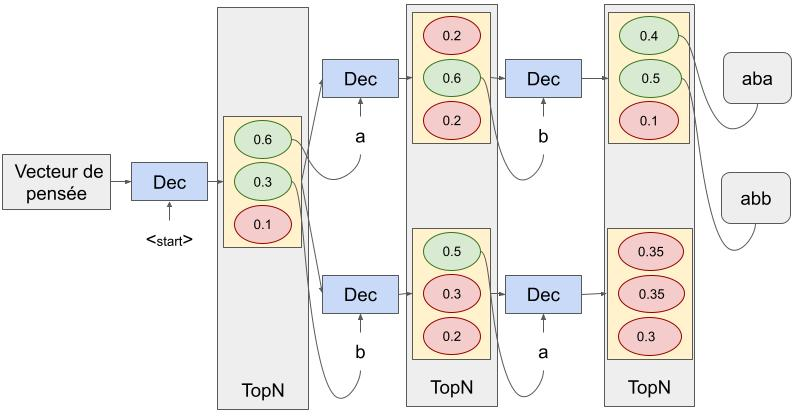
\includegraphics[scale=0.4]{2_production_mots_cles/Beam Search.jpg}
    \caption{Représentation schématique du processus de décodage grâce à l'algorithme de recherche en faisceau.}
    \label{fig:beam_search}
\end{figure}
\todo{refaire en tikz}

\`A l'inverse des algorithmes déterministes que nous avons décrits, notons l'existence des algorithmes d'échantillonnage. Ces algorithmes stochastiques choisissent les mots au hasard en fonction de leur probabilité. Les mots-clés générés par ces algorithmes ne sont donc pas reproductibles, ce qui dans le cadre de la production de mot-clés n'est pas souhaitable. Nous ne considérons donc pas cette technique.

\subsection{Paradigme encodeur-décodeur}\label{sub:paradigme_encodeur_decodeur}

Nous avons présenté dans les sections~\ref{sub:encoding} et \ref{sub:decoding} des moyens d'encoder des documents ainsi que des moyens de générer des séquences.
De nombreuses applications du traitement automatique de la langue nécessitent à la fois l'encodage d'une séquence et son décodage.
Par exemple dans le cadre de la traduction automatique, étant donnée une phrase en langue source, il faut la traduire dans une langue cible, c'est-à-dire qu'il faut encoder la phrase dans la langue source puis générer une phrase correspondante dans la langue cible.
Dans le cadre de la production de mots-clés, il faut générer un mot-clé en fonction d'un document.
Ainsi, le paradigme encodeur-décodeur introduit par \citet{sutskever_sequence_2014}, qui concatène un encodeur et un décodeur, permet de prendre en entrée une séquence de mots de longueur variable et de générer en sortie une autre séquence de mots de longueur variable.
Ce paradigme pallie la limite des réseaux de neurones présentés dans la section~\ref{sub:neural_network} (perceptrons mono ou multicouches) dont l'entrée et la sortie sont de taille fixe.

%Une fois une séquence encodée il est possible de la décoder, c'est-à-dire de produire un mot en fonction d'une représentation $h^t$.
%Générer un mot à partir d'une représentation $h_t$ consiste à passer la représentation dans un perceptron qui calcule une distribution de probabilité sur un vocabulaire, le mot à générer est choisis en fonction de sa probabilité.
    
%\begin{align}
    %\text{log}\: p(y|x) = \sum^m_{j=1} \text{log}\: p(y_j|y_{<j}, x)
%\end{align}

% FROM RECITAL SOTA

\colorlet{enccolor}{green!5}
\colorlet{inputcolor}{black!90!green}
\colorlet{deccolor}{blue!5}
\colorlet{outputcolor}{black!70!blue}
\colorlet{veccolor}{orange!15}
\colorlet{startendcolor}{black!60}
\colorlet{greybox}{black!3}

\begin{figure}[!htb]
\centering

\resizebox{\textwidth}{!}{%
\begin{tikzpicture}

\tikzstyle{cell}=[text centered, rectangle, draw, line width=.5pt, minimum height=1cm, minimum width=1.4cm, rounded corners=2pt]
\tikzstyle{word}=[font=\small\bfseries, text centered, minimum size=.5cm, minimum height=.3cm, text height=1.5ex, text depth=.25ex]
\tikzstyle{vector}=[text centered, rectangle, draw, line width=.5pt, minimum height=.5cm, minimum width=1cm, rounded corners=2pt]
\tikzstyle{arrow}=[shorten >= 2pt, shorten <= 2pt, draw=black!80]

\node[cell, fill=enccolor] (E1) at (0,0){};
\node[cell, fill=enccolor] (E2) at (2,0){};
\node[cell, fill=enccolor] (E3) at (4,0){};
\node[cell, fill=enccolor] (E4) at (6,0){};
\node[text centered] (E5) at (7.5,0){...};
\node[cell, fill=enccolor] (E6) at (9,0){};

\node[word, color=inputcolor, inner color=yellow!50, outer color=white] (I1) at (0,-1.2){Espace};
\node[word, color=inputcolor, inner color=yellow!50, outer color=white] (I2) at (2,-1.2){:};
\node[word, color=inputcolor, inner color=yellow!50, outer color=white] (I3) at (4,-1.2){la};
\node[word, color=inputcolor, inner color=yellow!50, outer color=white] (I4) at (6,-1.2){station};
%\node[word, color=inputcolor, inner color=yellow!50, outer color=white] (I5) at (8,-1.2){...};
\node[word, color=startendcolor] (I6) at (9,-1.2){<fin>};

%\node[cell, fill=veccolor, word, rotate=90] (V) at (11,0){vecteur de pensée};

\node[cell, fill=deccolor] (D1) at (11,0){};
\node[cell, fill=deccolor] (D2) at (13,0){};
\node[cell, fill=deccolor] (D3) at (15,0){};
%\node[cell, fill=deccolor] (D4) at (20,0){};

\node[word, color=startendcolor] (I7) at (11,-1.2){<début>};
\node[word, color=outputcolor, inner color=yellow!50, outer color=white] (O1) at (11,1.2){station};
\node[word, color=outputcolor, inner color=yellow!50, outer color=white] (O2) at (13,1.2){spatiale};
\node[word, color=startendcolor] (O3) at (15,1.2){<fin>};

\draw[->,>=latex,arrow] (E1) -- (E2) node[above,midway] {$h^e_0$};
\draw[->,>=latex,arrow] (E2) -- (E3) node[above,midway] {$h^e_1$};
\draw[->,>=latex,arrow] (E3) -- (E4) node[above,midway] {$h^e_2$};
\draw[->,>=latex,arrow] (E4) -- (E5) node[above,midway] {$h^e_3$};
%\draw[->,>=latex,arrow] (E5) -- (E6) node[above,midway] {$h^e_{n-1}$};
\draw[->,>=latex,arrow] (E5) -- (E6) node[above,midway] {$h^e_{n-1}$};

\draw[->,>=latex,arrow,shorten <= -2pt] (I1) to (E1);
\draw[->,>=latex,arrow,shorten <= -2pt] (I2) to (E2);
\draw[->,>=latex,arrow,shorten <= -2pt] (I3) to (E3);
\draw[->,>=latex,arrow,shorten <= -2pt] (I4) to (E4);
%\draw[->,>=latex,arrow,shorten <= -2pt] (I5) to (E5);
\draw[->,>=latex,arrow,shorten <= -2pt] (I6) to (E6);
\draw[->,>=latex,arrow,shorten <= -2pt] (I7) to (D1);


\draw[->,>=latex, arrow] (E6) -- (D1) node[above,midway] {$h^e_n$};

\draw[->,>=latex,arrow] (D1) -- (D2) node[above,midway] {$h^d_0$};
\draw[->,>=latex,arrow] (D2) -- (D3) node[above,midway] {$h^d_1$};
%\draw[->,>=latex,arrow] (D3) to (D4);

\draw[->,>=latex,arrow,shorten >= -2pt] (D1) to (O1);
\draw[->,>=latex,arrow,shorten >= -2pt] (D2) to (O2);
\draw[->,>=latex,arrow,shorten >= -2pt] (D3) to (O3);
%\draw[->,>=latex,arrow,shorten >= -2pt] (D4) to (O4);

%\node at (5,2) {\large{\textsc{Encodeur}}};
%\node at (17,2) {\large{\textsc{Décodeur}}};

\draw[arrow, rounded corners=3pt] (O1) -| (12, 0);
\draw[->,>=latex, arrow, rounded corners=3pt] (12, 0) -- (12, -1) -| (D2.south);

\draw[arrow, rounded corners=3pt] (O2) -| (14, 0);
\draw[->,>=latex, arrow, rounded corners=3pt] (14, 0) -- (14, -1) -| (D3.south);

%\draw[arrow, rounded corners=3pt] (O3) -| (19, 0);
%\draw[->,>=latex, arrow, rounded corners=3pt] (19, 0) -- (19, -1) -| (D4.south);

\draw[decoration={brace},decorate] (-0.7,1.7) -- node[below=-1.9em] {\large{\textsc{Encodeur}}} (9.7,1.7);
\draw[decoration={brace},decorate] (10.3,1.7) -- node[below=-1.9em] {\large{\textsc{Décodeur}}} (15.7,1.7);


\end{tikzpicture}
}

\caption{Exemple de modèle \textit{encodeur-décodeur} récurrent appliqué à l'extraction automatique de mots-clés.}
\label{fig:seq2seq}
\end{figure}


Le processus d'encodage et de décodage est décrit par l'équation~\ref{eq:enc-dec} et la figure~\ref{fig:seq2seq}.
Dans un premier temps la séquence d'entrée $X$ de taille $n$ est encodée dans le vecteur de pensée $h^e_n$.
Ce vecteur $h^e_n$ est utilisé pour initialiser le premier état caché du décodeur $h^d_0$.
Le décodeur génère ensuite les mots $\hat{y}_t$ qui composent la séquence de sortie $\hat{Y}$ à partir de cet état caché.

\begin{equation}\label{eq:enc-dec}
  \begin{split}
    p(\hat{y}_t | y_{1,...,t-1},h_0) & = \textsc{Softmax}(\sigma(b_v + W_v * h^d_t)) \\
    h^d_t & = \textsc{Rnn}^d(\hat{y}_{t-1}, h^d_{t-1}) \\
    \hat{y}_0 & = \textsc{Debut} \\
    h^d_0 & = h^e_n \\
    h^e_n & = \textsc{Rnn}^e(X) \\
  \end{split}
\end{equation}

Nous présentons ci-après deux améliorations de ce paradigme.
%
D'abord, le mécanisme d'attention qui permet de porter attention à une partie spécifique de l'entrée lors du décodage. Par exemple, la description d'une image nécessite d'identifier les différents objets qui la composent.
%
Ensuite, le mécanisme de copie qui pallie l'incomplétude du vocabulaire de sortie. Ce mécanisme permet au décodeur de copier un mot du document d'entrée au lieu de le générer à partir du vocabulaire de sortie. Le mécanisme de copie est particulièrement utile pour les entités nommées par exemple. Ces entités sont peu fréquentes et ne font généralement pas partie du vocabulaire de sortie.

% Convolution
%Les réseaux de neurones à convolution sont surtout utilisés pour le traitement d'images. Dans le cas du texte, des 
    
% Graphes
%Les réseaux à convolution de graphes (GCN) permettent d'obtenir pour chaque noeud d'un graphe un embedding en fonction de ses voisins. Le nombre de convolutions représente le nombre de bonds qui sont fait entre les noeuds.
    
% Transformer
%Les transformer ont été introduit par \cite{vaswani_attention_2017} et utilisent un mécanisme de self-attention pour chaque mot d'une séquence, de sorte à obtenir pour chaque mot un vecteur qui représente sa relation avec chaque autre mot. Ce mécanisme ne prend pas en compte la séquentialité, en effet chaque calcul est parallélisable. Et ce modèle qui requiert une force de calcul colossale a montré de très bons résultats sur de nombreuse tâches.

\subsubsection{Mécanisme d'attention}
\label{sub:attention_mecanism}

Le mécanisme d'attention~\cite{bahdanau_neural_2014,luong_effective_2015} a été introduit pour améliorer le traitement de longues séquences en permettant au modèle de se focaliser sur certaines parties du document lors du décodage.
%
En effet, un mot-clé concerne seulement certains aspects d'un document. Ce mécanisme permet donc au modèle de porter attention aux parties du document liées à ces aspects.
%
De plus, cette attention au document peut être visualisée grâce aux \emph{poids d'attention} calculés à chaque étape de décodage.
%Par exemple, dans le cadre de la traduction automatique, il permet de visualiser l'alignement entre la phrase en langue source et la phrase en langue cible.
%Par exemple, dans le cadre de la traduction automatique, ce mécanisme permet de visualiser l'importance de chaque mot du document source pour générer la traduction.
La figure~\ref{fig:attention_alignment} illustre cette attention dans le cadre de la traduction automatique pour traduire en français la phrase \say{The agreement on the European Economic Area was signed in August 1992.}
%Il existe généralement un alignement monotone entre les phrases en français et les phrases en anglais.
%Mais ce n'est pas toujours le cas comme le montre le syntagne nominal \say{European Economic Area} dont les mots de la traduction sont dans un ordre inverse \say{zone économique européenne}.
%Le modèle a pu, grâce au mécanisme d'attention, proposer la bonne traduction \say{zone économique européenne} dont l'ordre des mots est inverse à sa traduction.
% Même si le français et l'anglais peuvent généralemnt être traduit mot à mot de manière monotone, le mécanisme d'attention nous permet de visualiser l'alignement non monotone entre zone économique européenne et European Economic Area, en effet l'ordre des noms et adjectifs en français et en anglais est différent.
%Ainsi nous pouvons observer que pour traduire \say{was} en \say{a été}, le modèle à porté attention à \say{was signed} pour comprendre que \say{was} fait parti de la construction du prétérit.
%Pour illustrer ce mécanisme dans le cadre de la traduction automatique nous prenons l'exemple suivant: pour traduire la séquence \say{the European Economic Area} en français (\say{\foreign{la zone économique européenne}}) le modèle portera attention à chaque mot du texte source. Ainsi, pour générer \say{la} et \say{zone} il devra porter attention à \say{\foreign{the}} et \say{\foreign{Area}}. \todo{A revoir.}

\begin{figure}
    \centering
    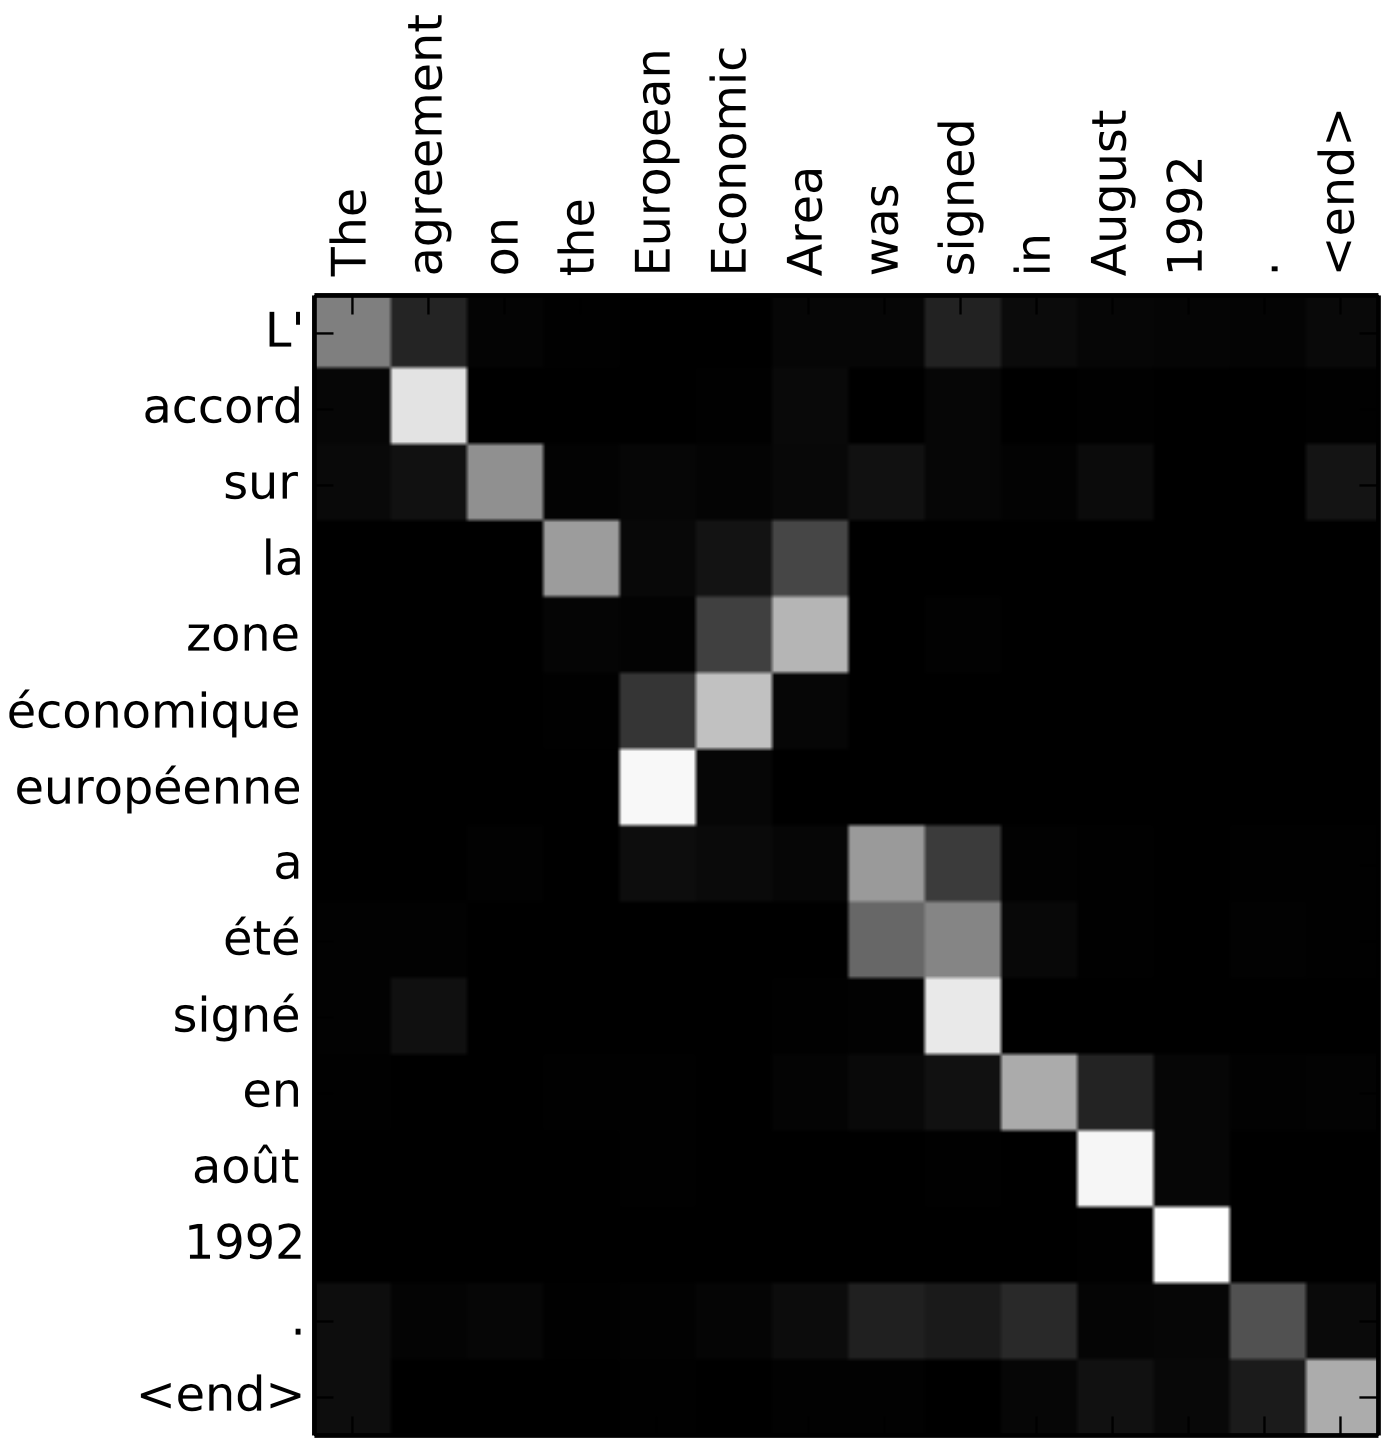
\includegraphics[scale=0.3]{2_production_mots_cles/attention_alignment.png}
    \caption{Exemple de visualisation des poids d'alignement du mécanisme d'attention entre une phrase en anglais et sa traduction en français. Chaque ligne montre la distribution des poids $\alpha_{t}$ ayant servis à générer le mot correspondant en français. Une case blanche indique un poids de 1, une case noire indique un poids de 0. Image extraite de \citet{bahdanau_neural_2014}.}
    \label{fig:attention_alignment}
\end{figure}

%Il faudra aussi porter attention à la syntaxe des deux langues
%Les poids d'attention peuvent être utilisés pour visualiser l'alignement entre les mots de la séquence d'entrée et ceux de la séquence de sortie.
%La figure~\ref{fig:attention_alignment} montre les poids d'alignement dans le cadre de la traduction automatique entre une phrase en anglais et sa traduction en français.

Le décodeur utilise l'état caché courant $h^d_t$ pour générer un mot, le mécanisme d'attention lui permet d'utiliser aussi tous les états cachés de l'encodeur $h^e$ pour mettre à jour l'état caché du décodeur $h^d_t$. Ce mécanisme est décrit dans l'équation~\ref{eq:attention}.
Dans le mécanisme d'attention, les états cachés $h^e$ sont pondérés en fonction de leur importance pour générer le mot $\hat{y}_t$.
Cette importance est établie grâce à une fonction d'alignement $a$ qui calcule une similarité entre l'état caché courant $h^d_t$ et ceux de l'encodeur $h^e$.
Les états cachés $h^e$ sont ainsi moyennés dans le vecteur de contexte $c_t$ utilisé pour mettre à jour l'état caché courant du décodeur $h^d_t$.

Dans l'équation \ref{eq:attention}: $[u;v]$ représente l'opération de concaténation des vecteurs $u$ et $v$; $a$ est une fonction d'alignement qui calcule la similarité entre un état caché de l'encodeur $h^e_t$ et du décodeur $h^d_t$; $\alpha$ représente les poids d'alignement entre les états cachés de l'encodeur $h^e$ et du décodeur $h^d$;  et $\textsc{Softmax}$ est une fonction qui normalise les valeurs d'un vecteur pour qu'il somme à 1.


\iffalse
    \begin{figure}
        \centering
        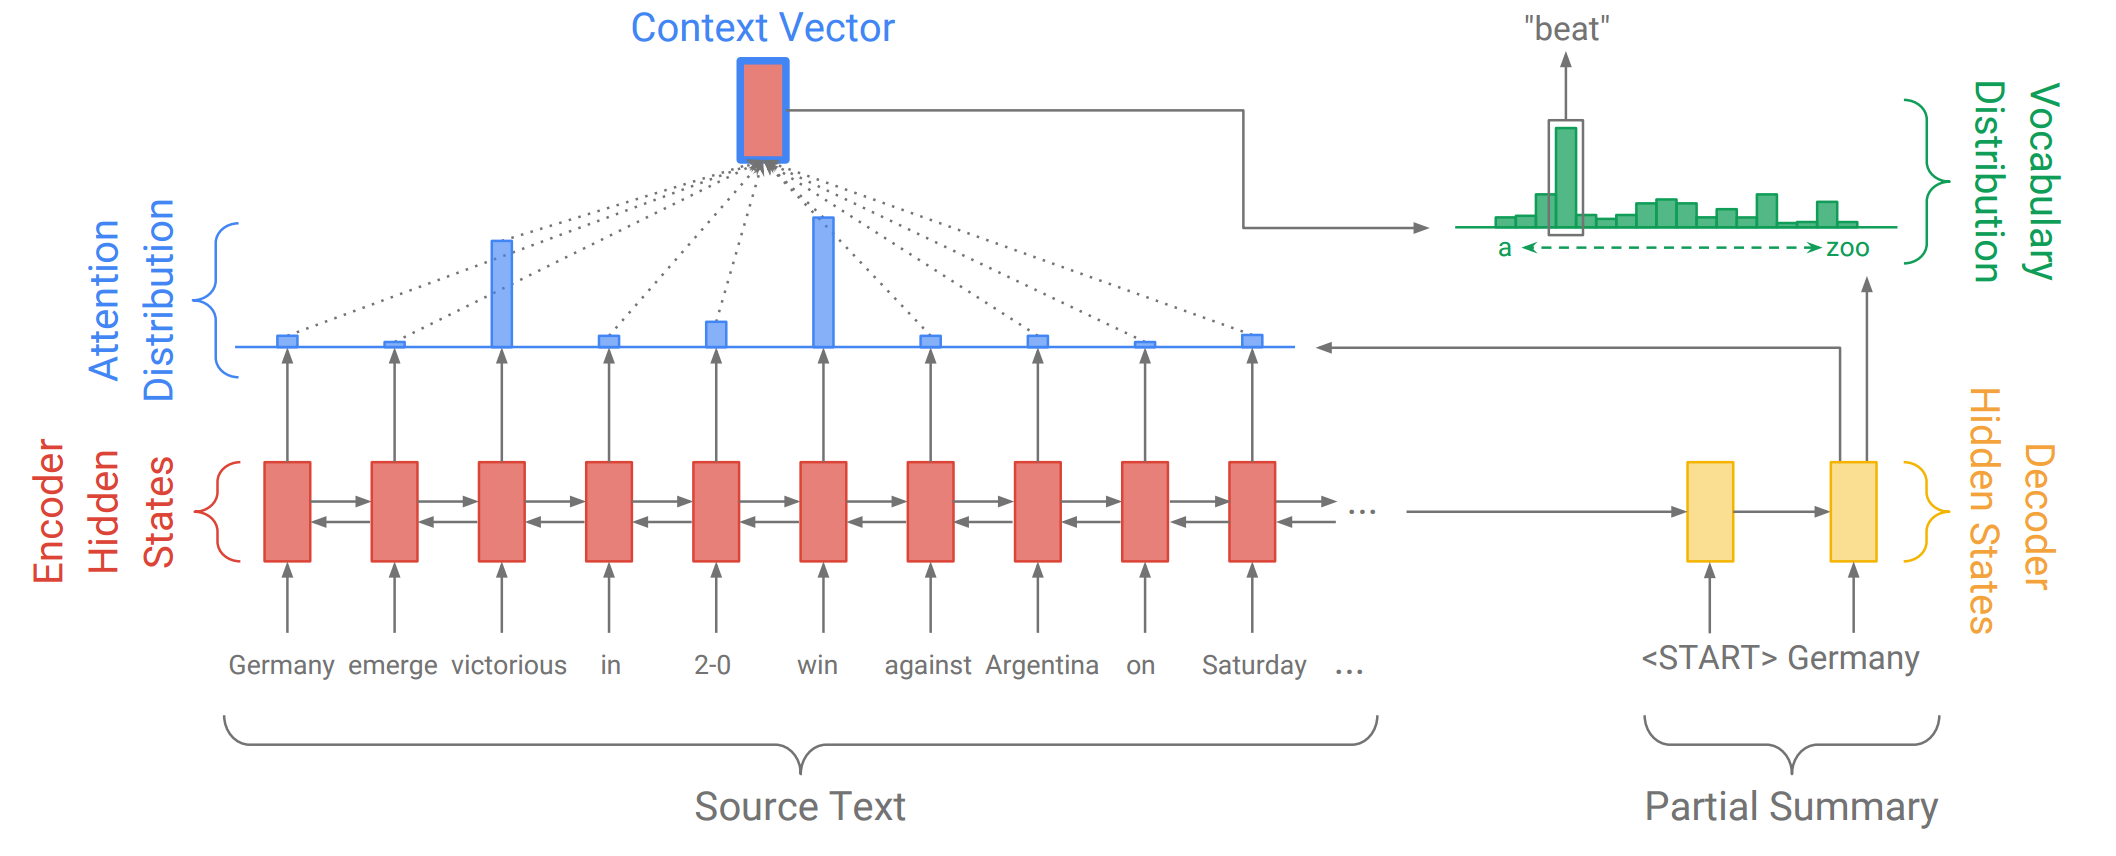
\includegraphics[width=\linewidth]{figures/see_seq2seq-attn.png}
        \caption{Schéma du mécanisme de copie présenté par \cite{see_get_2017}.}
        \label{fig:see_attention}
    \end{figure}
\fi

\begin{equation}\label{eq:attention}
  \begin{split}
    %\hat{Y}_t & = \sigma(b_v + W_v * h^d_t) \\
    p(y_t|y_{<t},x) & = \textsc{Softmax}(\sigma(W_v h^d_t)) \\[.3em]
    h^d_t & = \textsc{Rnn}(y_{t-1}, [h^d_{t-1};c_t]  \\[.3em]
    c_t & = \sum^{|h^e|}_{i=0} \alpha_{i,t} h^e_i \\
    \alpha_{t} & = \textsc{Softmax}(a(h^d_t, h^e)) \\
    %\textsc{Softmax}(x) & = \left[ \frac{x_i}{\sum^{|x|}_{i=0} x_i} , i \in |x| \right]
  \end{split}
\end{equation}

%Le concept d'attention a été présenté de deux manières différentes par \cite{bahdanau_neural_2014} et \cite{luong_effective_2015}.
%
%L'idée de l'attention présentée par~\cite{luong_effective_2015} est \emph{d'utiliser le vecteur de contexte pour prédire $y_t$}.
%
%\cite{bahdanau_neural_2014} présente un autre mécanisme d'attention dont l'idée est de calculer l'état caché du décodeur à l'aide d'un vecteur de contexte. Par rapport à un décodeur classique, seul le calcul de $h^d_t$ change.

\iffalse
    L'idée de l'attention présentée par~\cite{luong_effective_2015} est \emph{d'utiliser le vecteur de contexte pour prédire $y_t$}.
    
    Pour cela, un nouveau $\hat{h}^d_t$ est calculé en fonction d'un vecteur de contexte $c_t$ et de $h^d_t$ (calculé en fonction de $y_{t-1}$ et $h^d_{t-1}$). $c_t$ est la moyenne des $h^e$ pondérés par les scores d'alignement $\alpha$.
    
    Dans leur article, deux manières de calculer l'attention sont présentées: une attention globale et une attention locale.
    %
    Pour l'attention globale, le vecteur de contexte est la moyenne pondérée de toutes les représentations de l'encodeur.
    %
    Pour l'attention locale, le vecteur de contexte est la moyenne pondérée des représentations $h^e$ dans une fenêtre de taille $D$ autour de $h^e_{p_t}$.
    %
    $p_t$ est une valeur entre 0 et $|h^e|$ qui définit le centre de la fenêtre, et peut être calculé de différentes manières.\footnote{Pour plus de détails voir la section 3.2 de \cite{luong_effective_2015}}
    %$p_t$ étant $t$ (dans la traduction automatique on considère que le mot cible $y_t$ est aligné avec le mot source $x_{p_t}$), ou alors un réel entre 0 et $|h^e|$ calculé à l'aide 
    
    \begin{align}
        %y_t & = \sigma(W_v h^d_t) \\
        p(y_t | y_{<t}, x) & = \textsc{Softmax}(W_v \hat{h}^d_t) \\
        \hat{h}^d_t & = \sigma(W_c [c_t;h^d_t]) \\
        c_t & = \sum^{|h^e|}_{i=0} \alpha_{i,t} * h^e_i \\
        \alpha_{i,t} & = \textsc{Softmax}(a(h^e_i, h^d_t)) \\
        h^d_t & = \textsc{Rnn}(y_{t-1}, h^d_{t-1})
    \end{align}
    
    \cite{bahdanau_neural_2014} présente un autre mécanisme d'attention dont l'idée est de calculer l'état caché du décodeur à l'aide d'un vecteur de contexte. Par rapport à un décodeur classique, seul le calcul de $h^d_t$ change. Le calcul du vecteur de contexte est similaire à celui de ~\cite{luong_effective_2015}.
    
    \begin{align}
        p(y_t|y_{<t},x) & = \textsc{Softmax}(W_v h^d_t) \\
        h^d_t & = \textsc{Rnn}(y_{t-1}, [h^d_{t-1};c_t]  \\
        c_t & = \sum^{|h^e|}_{i=0} \alpha_{i,t} * h^e_i \\
        \alpha_{i,t} & = \textsc{Softmax}(a(h^e_i, h^d_t))
    \end{align}
    
    Il existe différentes fonctions d'alignement:
    
    bahdanau $a(h^e_i, h^d_t) = v_a \text{tanh}(W_a h^d_t + U_a h^e_i)$
    
    dot $a(h^e_i, h^d_t) = h^e_i h^d_t$
    
    general $a(h^e_i, h^d_t) = h^e_i W_a h^d_t$
    
    concat $a(h^e_i, h^d_t) = W_a [h^e_i;h^d_t]$
\fi

\subsubsection{Mécanisme de copie}
\label{sub:copy_mecanism}

Le mécanisme de copie~\cite{see_get_2017,gu_incorporating_2016} provient des tâches de traduction automatique et de résumé automatique. Il a pour but de produire des mots peu fréquents ou hors du vocabulaire de sortie.
En effet, les modèles neuronaux qui génèrent du texte choisissent les mots dans un vocabulaire de sortie comportant généralement \num{50 000} mots.
Dans les tâches sus-citées, les mots peu fréquents qui ne font pas partie du vocabulaire de sortie, comme les entités nommées ou les transfuges, doivent pourtant apparaître dans la séquence de sortie.
%Le mécanisme de copie ~\cite{see_get_2017,gu_incorporating_2016} pallie ce problème en permettant au décodeur de générer un mot du vocabulaire de sortie ou bien de copier un mot du document.
Deux mécanismes de copie ont été proposés par \citet{see_get_2017} et \citet{gu_incorporating_2016}; les deux étant similaires, nous présentons ici le premier car plus simple. Il est décrit dans l'équation~\ref{eq:copy_mecanism}.

% exemple
%Le mécanisme d'attention a été utilisé comme post-traitement pour remplacer les mots inconnus de la sortie par les mots de l'entrée alignés par le mécanisme d'attention. Ceci permettant de traiter les entités nommées peu fréquentes ou les transfuges.
%
%Le mécanisme de copie vient automatiser ce processus en permettant au modèle de générer un mot du vocabulaire ou de copier un mot du document.

%, tous deux inspirés des réseaux de pointeurs~\cite{vinyals_pointer_2015} qui génèrent une séquence de pointeurs vers la séquence d'entrée.
Ce mécanisme utilise le vocabulaire de la séquence d'entrée $\mathcal{X}$ (particulier à chaque document) en plus du vocabulaire de sortie $\mathcal{V}$.
Pour produire un mot, une distribution de probabilité sur le vocabulaire  $P_{vocab}(y_{t})$ est calculée comme précédemment par le décodeur (cf. section~\ref{sub:decoding}) et les poids du mécanisme d'attention $\alpha$ (cf. section~\ref{sub:attention_mecanism}) sont utilisés pour estimer la probabilité de copie de chaque mot du document.
Les poids d'attention $\alpha$ des mots qui apparaissent plusieurs fois dans l'entrée $x$ sont sommés $\sum_{j,x_j=y_{t,i}} \alpha^t_j$.
Ainsi, un mot peut être généré à partir du vocabulaire de sortie $\mathcal{V}$ ou copié à partir du vocabulaire du document $\mathcal{X}$.
Les probabilités de copie et de génération d'un même mot, qui appartient au document et au vocabulaire, sont sommées.
Dans l'équation~\ref{eq:copy_mecanism}: $h^d_t$, $c_t$ et $\alpha^t_j$ proviennent du mécanisme d'attention (cf. équation~\ref{eq:attention}); $p_{gen}$ est un curseur permettant au modèle de privilégier la copie ou la génération et $P_{vocab}(y_t)$ est une distribution de probabilité sur le vocabulaire de sortie $\mathcal{V}$.

%Les probabilités de génération et de copie sont combinés pour donner une distribution de probabilités sur $\mathcal{X} \cup \mathcal{V}$.

\begin{equation}\label{eq:copy_mecanism}
  \begin{split}
    p(y_{t,i}|y_{<t},x) & = p_{gen} P_{vocab}(y_{t,i}) + (1 - p_{gen}) \sum_{j,x_j=y_{t,i}} \alpha^t_j \\
    p_{gen} & = \sigma(W_h h^d_t + W_c c_t + W_y y_{t-1}) \\
    P_{vocab}(y_{t}) & = \textsc{Softmax}(\sigma(W_v h^d_t))
  \end{split}
\end{equation}

%ou les poids d'un mécanisme d'attention supplémentaire, utilisé seulement pour calculer le score de copie, pour~\cite{gu_incorporating_2016}

\iffalse
    %\cite{gu_incorporating_2016}, création d'un vocabulaire spécifique a chaque instance, composé de $\mathcal{V}$ le vocabulaire normal et $\mathcal{X}$ le vocabulaire des mots de l'entrée.
    %
    %Ça change le calcul de $y_t$ par rapport au mécanisme d'attention.
    %
    %On défini les vecteurs $\psi_g \in \mathds{R}^|\mathcal{V}|$ et $\psi_c \in \mathds{R}^|\mathcal{X}|$ qui contiennent respectivement les score de copie et de génération.
    
    % attentive read = les poids de l'attention
    % selective read = les poids de l'"attention" du mécanisme de copie
    
    \begin{align}
        y_t & = \textsc{Softmax}(e^{P_{gen}} +e^{P_{copy}}) \\
        P_{gen} & = W_v h^d_t \\
        P_{copy} & = \left[ \sum^{|h^e|}_{j=0, x_j=x_i} \sigma(h^e_j W_c) h^d_t | x_i \in \mathcal{X} \right] \\
        h^d_t & = RNN([y_{t-1};cc_t)],h^d_{t-1}) \\
        cc_t & = \sum^{|h^e|}_{i=1} aa_{t,i} h^e_t \\
        aa_{t,i} & = \textsc{Softmax}()
    \end{align}
    
    %\cite{see_get_2017} reprend le mécanisme d'attention de \cite{luong_effective_2015} et modifie le calcul de $y_t$ en ajoutant une probabilité de copie et un curseur privilégiant la copie ou la génération.
    
    \begin{align}
        p(y_{t,i}) = p_{gen} P_{vocab}(y_{t,i}) + (1 - p_{gen}) \sum_{j,x_j=y_{t,i}} \alpha^t_j \\
        p_{gen} = \sigma(W_c c_t + W_h h^d_t + W_y y_{t-1})
    \end{align}
\fi

% Multitache
% Conditional Random Field
% Reinforcement Learning : adaptative reward


\section{Méthodes de bout-en-bout}
\label{methodes-de-bout-en-bout}

\todo{Ajouter des schéma pour mieux comprendre les méthodes.}

Dans cette section nous présentons un état de l'art des méthodes de bout-en-bout.
Ces méthodes, contrairement aux méthodes en chaîne de traitement (cf. section~\ref{sec:methode-en-chaine-de-traitement}), prennent en entrée un document et laissent le soin au modèle d'en extraire les caractéristiques pour retourner un ensemble de mots-clés sans étapes intermédiaires ni définition manuelle de ces caractéristiques.
Parmi les méthodes proposées dans la littérature, nous distinguons les méthodes génératives, qui peuvent produire des mots-clés présents et des mots-clés absents, des méthodes extractives, limitées aux mots-clés présents.

Jusqu'à présent, toutes les méthodes de bout-en-bout qui ont été proposées sont supervisées et reposent sur des réseaux de neurones (cf. section~\ref{sub:neural_network}) qui nécessitent de grandes quantités de données annotées pour être entraînées.
%
Le développement de ces méthodes démarre avec l'introduction du jeu de données KP20k et de la méthode générative CopyRNN par \citet{meng_deep_2017}.
Le jeu de données KP20k, qui comporte $\simeq$\num{550000} documents, comble un manque.
En effet, seuls de petits jeux de données (de l'ordre du millier de documents) étaient jusqu'alors disponibles.
Ce travail a ainsi lancé une nouvelle direction de recherche sur les méthodes génératives de production de mot-clés.

\begin{figure}
    \centering
    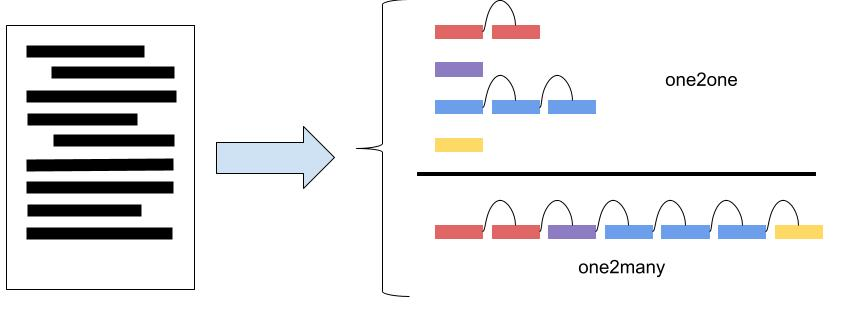
\includegraphics[scale=0.4]{2_production_mots_cles/Decoding strategies.jpg}
    \caption{Représentation schématique des stratégies de décodage \emph{one2one} et \emph{one2many}.}
    \label{fig:decoding_strategies}
\end{figure}
\todo{Refaire en tikz}

Dans cet état de l'art, nous présentons tout d'abord les méthodes automatiques de génération de mots-clés de bout-en-bout, qui sont au c\oe{}ur de ce travail de thèse.
Nous présentons ces méthodes de génération en deux parties: premièrement, les méthodes qui générent les mots-clés un à un (\emph{one2one}), et deuxièmement, celles qui génèrent des séquences de mots-clés (\emph{one2many}). Ces deux types de génération sont schématisés dans la figure~\ref{fig:decoding_strategies}.
Nous présentons ensuite les méthodes extractives de bout-en-bout, c'est-à-dire celles qui se limitent aux seuls mots-clés présents.

\subsection{Génération de mots-clés}
\label{sub:generation_de_mots_cles}

Les méthodes génératives, introduites par \citet{meng_deep_2017}, ont pour objectif de pallier deux faiblesses qui concernent la majorité des méthodes extractives présentées précédemment: l'impossibilité de produire des mots-clés absents ainsi que la faible prise en compte de la sémantique.
Le paradigme encodeur-décodeur sur lequel les méthodes génératives sont fondées permet d'encoder la sémantique du document.
Ainsi, les mots-clés produits sont le fruit d'une \say{compréhension} du document, contrairement aux méthodes en chaîne de traitement qui s'intéressent à l'\say{importance} des mots dans le document indépendamment de leur sens.
%
Ces méthodes génératives rendent possible la production de mots-clés absents grâce à la manière dont le décodeur génère la séquence de sortie.
Ce processus s'effectue en choisissant, à chaque étape de décodage, un mot à partir d'un vocabulaire de sortie qui est plus grand et différent du vocabulaire du document.
Ces méthodes génératives apprennent à générer des mots-clés un par un (génération \emph{one2one}, voir figure~\ref{fig:decoding_strategies}), c'est-à-dire que chaque document $X$ et son ensemble de mot-clés $Y$ de taille $N$ forment un couple $(X, \{Y_0, ..., Y_N\})$, décomposé en autant d'exemples d'entraînement que de mots-clés, $(X, Y_0), ... , (X, Y_N)$.

%\paragraph{Définitions}
%\todo{Il faudrait définir avant les principaux modèles: one2one, séquence avant de les définir formellement; Fait ausi des dessins}
%$x$ et $y$ représentent des mots, $p$ des mots-clés. Étant donné un ensemble de données $D = {(x^i,p^i), i \in 1...N}$ de taille $N$, un exemple est composé d'un document $x^i$ et d'un ensemble de mots-clés $p^i = {p^i_j, j \in 1...M^i}$ de taille $M^i$. Les documents et les mots-clés sont composés de mots $[x^i_k, k \in 1...N^i]$ et $[y^i_j]$ est composé d'un document composé d'une séquence de mots $x^i = (x^i_1, ..., x^i_{N^i})$ de longueur $N^i$ et d'un ensemble de mots-clés $p^i$ de taille $M^i$ avec $p^i = (p^i_1, ..., p^i_{M^i})$, où chaque mot-clé est une séquence de mots de taille $M^{i,j}$ avec $p^{i,j} = (y^{i,j}_1, ..., y^{i,j}_{M^{i,j}})$. Dans le cadre des modèles one2one, un couple document -- mots-clés est découpé en $M^i$ différents couples $(x^i, p^{i,1}), ..., (x^i, p^{i, M^i})$. 
%Pour les modèles en séquences, les mots-clés sont concaténés de sorte à former une unique séquence $(x^i, y^{i,1}_1 \lozenge ... \lozenge y^{i,1}_{M^{i,j}} \lozenge \text{SEP} \lozenge y^{i,2}_1 \lozenge ... \lozenge y^{i,M^i}_{M^{i,j}})$.

La méthode pionnière de génération automatique de mots-clés appliquée aux documents scientifiques est CopyRNN~\cite{meng_deep_2017}.
%
L'architecture neuronale de cette méthode s'inspire du processus d'annotation humain qui consiste à lire le document pour le comprendre dans son entièreté puis à le résumer grâce à des mots-clés.
%Aussi, les humains peuvent facilement s'abstraire du texte et faire appel à leurs connaissances pour produire des mots-clés qui n'apparaissent pas dans le texte.
Pour reproduire ce processus, CopyRNN utilise le paradigme encodeur-décodeur, que nous avons présenté dans la section~\ref{sub:paradigme_encodeur_decodeur}, pour encoder un document et le décoder ensuite en un mot-clé. % Ainsi un réseau de neurones récurrent encode le document dans un vecteur de pensée, puis un autre décode, génère, ce vecteur de pensée en un mot-clé.
Pour améliorer les performances des modèles encodeur-décodeur, il est commun d'utiliser un mécanisme d'attention (voir section~\ref{sub:attention_mecanism}).
Ce mécanisme permet au modèle de porter attention à certaines parties du document lors de la génération d'un mot.
%
Un mécanisme de copie est aussi ajouté au modèle pour lui permettre de générer des mots peu fréquents (voir section~\ref{sub:copy_mecanism}).
Ce mécanisme de copie modifie le décodage en permettant de générer un mot à partir du vocabulaire de sortie ou bien à partir du document.\\
%
Cette méthode obtient des performances bien plus élevées que les précédentes méthodes extractives. Les performances de CopyRNN sont de l'ordre de 30 points de \fmesure{} pour les mots-clés présents tandis que les performances des méthodes extractives sont généralement en dessous de 20 points de \fmesure{}.
Les mots-clés absents, qui ne pouvaient jusque-là pas être produits, correspondent peu à la référence: parmi les 50 meilleurs mots-clés absents un seul apparaît dans la référence.


%La communauté scientifique présente de nouvelles méthodes basées sur CopyRNN et tente de l'améliorer.
% les méthodes essaient de résoudre les problèmes identifiés
%Les méthodes présentées augmentent toujours les performances de génération des mots-clés présents et absents.

Certaines méthodes proposées essaient d'améliorer l'encodage du document.
\citet{chen_title-guided_2019}, par exemple, constate que les mots-clés ne sont pas uniformément distribués dans les documents.
En particulier \npercent{60} des mots-clés de référence ont au moins un mot en commun avec le titre du document.
Pour prendre cela en compte, ils proposent TGNet (Title Guided Network), qui étend CopyRNN en introduisant un nouvel encodeur spécifique au titre, en plus de l'encodeur du document.
Cet encodage du titre permet de donner un poids supplémentaire à l'information qu'il contient.
Ces deux représentations (du titre et du document) sont ensuite combinées puis fournies au décodeur.
Cette méthode améliore nettement les performances de génération des mots-clés présents et absents par rapport à CopyRNN (+\npercent{5} sur KP20k).
% Ils ne regardent que la F-mesure présent/absent rien d'autre

La redondance dans les ensembles de mots-clés produits est un problème récurrent dans les méthodes de production de mots-clés.
En effet, \citet{hasan_automatic_2014} montrent que 8 à \npercent{12} des erreurs des méthodes sont liées à la redondance des mots-clés.
Ainsi, les méthodes en chaîne de traitement mettent en place des stratégies, notamment lors de la sélection du sous-ensemble de mots-clés, pour limiter cette redondance (voir section~\ref{choisir-le-sous-ensemble}).
Dans cette ligne de recherche, \citet{zhao_incorporating_2019} remarquent les méthodes de bout-en-bout ne sont pas exemptes de ce problème, ils s'intéressent ainsi au chevauchement entre les mots-clés générés et ceux de référence.
Par exemple, \npercent{23.98} des mots-clés unigrammes générés par CopyRNN font partie d'un mot-clé de référence, et \npercent{47.15} des mots-clés 4-grammes générés par CopyRNN contiennent un mot-clé de référence.
Dans l'optique de limiter ces chevauchement, ils présentent le modèle ParaNet$_T$+CoAtt qui entraîne le modèle, à générer à la fois les mots-clés et leurs étiquettes morphosyntaxiques, ainsi la syntaxe des mots-clés générés sera similaire à celle des mots-clés de référence.
Pour cela ils ajoutent au modèle CopyRNN un encodeur, pour les étiquettes morphosyntaxiques des mots du document, ainsi qu'un décodeur, pour celles du mot-clé.\footnote{Les étiquettes morphosyntaxiques du document et des mots-clés proviennent de l'outils Stanford CoreNLP.}
Les informations des deux décodeurs sont ensuite combinées et utilisées pour générer les mots-clés et leurs étiquettes morphosyntaxiques.
%Grâce à cette méthode, les mots-clés générés chevauchent moins les mots-clés de référence; par exemple le pourcentage de mot-clés 4-grammes contenant un mot-clé de référence a baissé de \npercent{10}.

\begin{figure}
    \centering
    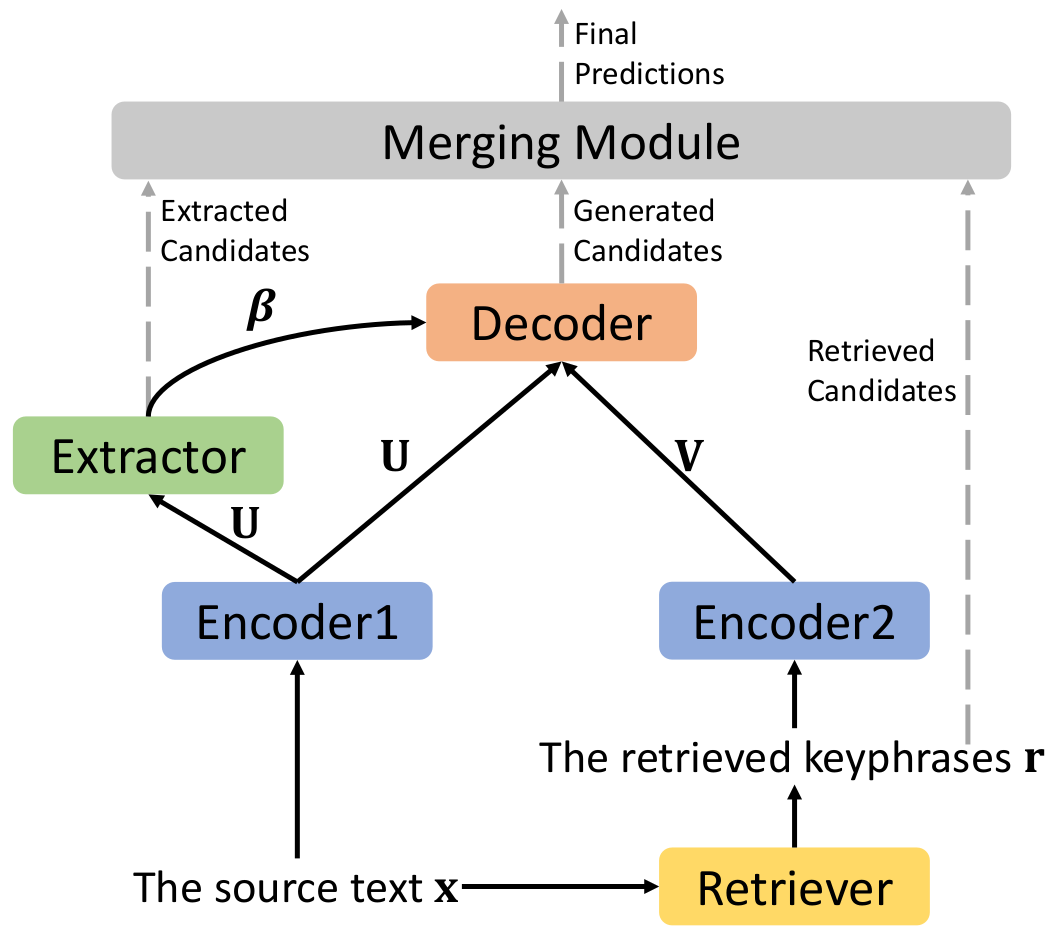
\includegraphics[scale=0.2]{2_production_mots_cles/kg_ke_kr_m.png}
    \caption{Représentation schématique de l'architecture de la méthode KG-KE-KR-M. Image extraite de~\citet{chen_integrated_2019}.}
    \label{fig:schema_kgkekrm}
\end{figure}

%Le processus manuel d'annotation en mots-clés est composé de plusieurs étapes: la lecture du document, l'extraction des mots-clés dans le document puis l'attribution de mots-clés absents du document et enfin la combinaison des mots-clés provenant de ces deux processus d'annotation.
Dans l'optique de reproduire l'annotation humaine, \citet{chen_integrated_2019} propose la méthode KG-KE-KR-M qui produit un ensemble de mots-clés en combinant différentes méthodes: génération de mots-clés, extraction de mots-clés, récupération de mots-clés (voir figure~\ref{fig:schema_kgkekrm}).
%Ces différentes méthodes sont entraînées de bout-en-bout puis les mots-clés de chaque méthode sont pondérés grâce à un classifieur.
%
Dans un premier temps, cette méthode récupère les mots-clés de référence des $K$ documents d'entraînement les plus proches du document traité (grâce à la distance de Jaccard).
Ces mots-clés \emph{récupérés} sont concaténés puis encodés. Ils serviront à conditionner la génération de mots-clés.
Dans un second temps, des mots-clés sont \emph{extraits} du document en classifiant chaque mot comme mot-clé ou non mot-clé.
%Cette classification s'effectue grâce aux états cachés du document encodé.
Ensuite, des mots-clés sont \emph{générés} à partir du document ainsi que des mots-clés récupérés et des mots-clés extraits.
Enfin, les mots-clés récupérés, extraits et générés sont pondérés grâce à un classifieur.
Cette méthode à la particularité de combiner les méthodes en chaîne de traitement (sélection de candidats puis pondération) et les méthodes de bout-en-bout (apprentissage conjoint de la génération et de l'extraction).
Malgré la grande diversité dans les techniques de production de mots-clés candidats, les performances ne sont pas significativement supérieures à CopyRNN. Cette méthode produit néanmoins plus de mots-clés absents de référence que CopyRNN.

La méthode CorrRNN~\cite{chen_keyphrase_2018} considère que les mots-clés doivent couvrir l'ensemble des sujets du document et être divers, c'est-à-dire que chaque mot-clé doit concerner un sujet différent.
Cette méthode étend CopyRNN en y ajoutant un mécanisme de couverture et un mécanisme de revue.
Le mécanisme de couverture encourage le modèle à porter attention aux différentes parties du document.
Il conserve et accumule les scores d'attention des mots du document à chaque étape de décodage, et il est inclus dans le calcul du mécanisme d'attention.
Ensuite, le mécanisme de revue est essentiellement un mécanisme d'attention sur les mots générés.
Son objectif est d'identifier les sujets déjà couverts par les mots-clés générés et ainsi de générer des mots-clés qui concernent des sujets non traités.
Cette méthode est la première à prendre en compte les mots-clés déjà générés dans le processus de génération, pour cela la phase d'entraînement est modifiée.
Au lieu de rétro-propager le gradient après chaque mot-clé de référence, la phase de rétro-propagation n'est effectuée qu'une fois tous les mots-clés de référence du document traités.
%Chaque mot-clé est généré en utilisant les mécanismes de couverture et de redondance, qui prennent en compte les mots-clés déjà générés; le gradient est ensuite calculé grâce à l'erreur de chaque mot-clé; et enfin, rétro-propagé.
%Cette méthode améliore les performance de production de mots-clés présent par rapport à CopyRNN, mais l'article ne présentant pas ses résultats sur le jeu de données de référence KP20k et utilisant des métriques peu utilisés dans les autres travaux la comparaison est limitée.

\subsection{Génération de séquences de mots-clés}% (\textsc{One2Seq})}
%\subsection{Génération en séquence}
\label{sub:generation_de_sequences_de_mots_cles}

%Nous avons présenté dans la section précédente, des méthodes génératives qui apprennent à générer un mot-clé par document.
Nous présentons dans cette section des méthodes qui apprennent à générer des séquences de mots-clés (génération \emph{one2many}, voir figure~\ref{fig:decoding_strategies}). C'est-à-dire que chaque exemple d'entraînement est composé d'un document et de la concaténation des mots-clés de référence en une unique séquence dans laquelle ils sont séparés par un symbole de séparation. Par exemple, l'ensemble de mots-clés $\{$ Classe , Fichier log , Agrégat $\}$ sera transformé en \say{Classe \texttt{SEP} Fichier log \texttt{SEP} Agrégat \texttt{FIN}}.
%Le développement des méthodes utilisant la génération \emph{one2many} part du constat que la génération \emph{one2one} ne permet pas de prendre en compte les mots-clés déjà générés et que les ensembles de mots-clés sont souvent redondants~\cite{hasan_automatic_2014}.
Le développement des méthodes génératives \emph{one2many} part du constat que les ensembles de mots-clés produits sont souvent redondants~\cite{hasan_automatic_2014} et que la génération \emph{one2one} ne permet pas de pallier ce problème.
En effet, les méthodes \emph{one2many} font l'hypothèse qu'avec la génération en séquence, le modèle ayant accès aux mots-clés déjà générés, il ne générera pas de mots-clés redondants.
%
Cette méthode de génération permet au modèle de générer le même nombre de mots-clés que la référence, en effet, il apprend en même temps qu'à générer les mots-clés, à placer les séparateurs de mots-clés et le symbole de fin.
Ainsi, ces méthodes peuvent générer des mots-clés selon deux stratégies~\cite{yuan_one_2020}: l'\textbf{inférence exhaustive} qui utilise l'algorithme de recherche en faisceau pour sur-générer des mots-clés et ainsi en obtenir un nombre fixe pour chaque document, c'est la stratégie employée par les méthodes génératives \emph{one2one}; et l'\textbf{inférence auto-régulée} (\foreign{self-terminating}) dans laquelle le décodage s'arrête lors de la génération du symbole de fin, cette stratégie permet au modèle de produire un nombre pertinent de mots-clés pour le document.
La seconde stratégie de décodage permet donc de s'affranchir du choix arbitraire du nombre de mots-clés $n$ à produire (voir section~\ref{choisir-le-sous-ensemble}).

Pour entraîner ces modèles, les mots-clés sont concaténés, mais ce processus n'est pas trivial.
En effet, l'ordre dans lequel les mots-clés sont concaténés influence les performances des modèles.
L'étude de \citet{meng_empirical_2021} compare différentes manières d'ordonner les mots-clés, telles que: \emph{No-Sort} qui laisse l'ordre par défaut; \emph{Alpha} qui trie par ordre alphabétique; \emph{Pres-Abs} qui place les mots-clés présents avant les mots-clés absents. L'étude montre que c'est l'ordre \emph{Pres-Abs} qui donne les meilleures performances.

La première méthode à générer des séquences de mots-clés est catSeqD~\cite{yuan_one_2020,yuan_generating_2018}.
L'objectif de cette méthode, similaire à CorrRNN, est d'augmenter la diversité des mots-clés générés.
%
Pour cela, le modèle CopyRNN, utilisé comme base, est augmenté d'un mécanisme de couverture sémantique et de régularisation orthogonale pour former le modèle catSeqD.
%
Le mécanisme de \emph{couverture sémantique} repose sur l'hypothèse que l'ensemble de mots-clés de référence et le document encodent la même information.
Ainsi, un nouvel encodeur est entraîné à encoder les mots-clés et à produire la même représentation que pour le document.
Il encode la séquence au fur et à mesure de sa génération et l'état cachés qui en résulte conditionne la prédiction du mot suivant, cela contraint les mots-clés générés à être proche sémantiquement du document.
%
Ensuite, les auteurs constatent que les mots générés après les séparateurs de mots-clés sont souvent similaires.
Le mécanisme de \emph{régularisation orthogonale} pallie ce problème en diversifiant explicitement les représentations des séparateurs, en pénalisant, dans la fonction de coût, ces représentations si elles ne sont pas orthogonales.

\todo{Refaire en Tikz}
\begin{figure}
    \centering
    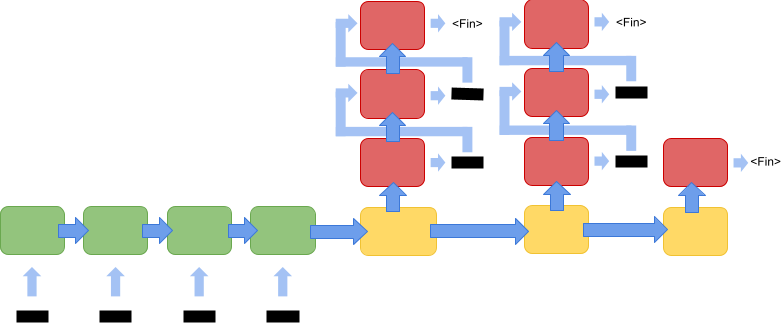
\includegraphics[scale=0.5]{2_production_mots_cles/exhird.png}
    \caption{Représentation schématique du décodage hiérarchique de la méthode ExHirD. L'encodeur du document est représenté en vert, le décodeur de concept en jaune et le décodeur de mots-clés en rouge.}
    \label{fig:schema_exhird}
\end{figure}

Dans le but de mieux modéliser les ensembles de mots-clés, \citet{chen_exclusive_2020} s'intéressent à la structure hiérarchique des ensembles de mots-clés.
En effet, les méthodes de génération de séquences de mots-clés identifient les mots-clés grâce à des marqueurs générés par le modèle. Cette séquentialité ne permet pas de représenter la hiérarchie entre les mots-clés et les mots qui les composent.
Ces travaux se rapprochent de \citet{yuan_generating_2018} qui essaient de rompre la séquentialité en modifiant la représentation des séparateurs de mots-clés avec le mécanisme de régularisation orthogonale.
Ainsi, ils présentent la méthode ExHirD~\cite{chen_exclusive_2020} dans laquelle le décodeur de l'architecture de CopyRNN est remplacé par un décodeur hiérarchique (voir figure~\ref{fig:schema_exhird}) qui génère les mots-clés en deux temps: d'abord l'identification des concepts, ensuite la génération de leur représentation textuelle.
Ce décodeur hiérarchique comprend un premier décodeur qui produit une représentation dense d'un concept, puis un second décodeur qui va générer une séquence de mots à partir de cette représentation dense pour instancier le concept en un mot-clé.
La génération des mots utilise deux mécanismes d'attention sur les documents d'entrée: l'un est conditionné par la représentation dense du concept; l'autre, standard, est conditionné par le mot précédent.
Ainsi, ce décodeur hiérarchique permet de modéliser explicitement les concepts importants du document et les mots qui les décrivent.
%
L'évaluation de cette méthode montre néanmoins un faible gain de performance, de l'ordre d'un point de F@5, pour les mots-clés présents et absents.
%
Ces travaux s'attellent aussi au problème de redondance des mots-clés et proposent un mécanisme de décodage exclusif pour tenter de le résoudre.
Ce mécanisme, simple dans son idée, interdit au modèle de générer deux mots-clés commençant par le même mot.
En effet, les mots-clés comportent le plus souvent entre 1 et 4 mots (voir section~\ref{sub:nature_linguistique}), ainsi le premier mot affecte grandement les suivants.
Ce mécanisme n'est pas limité à la méthode ExHirD; il peut être adapté aux différents types de décodage ou être utilisé en post-traitement.
Son évaluation montre qu'il fait significativement baisser le nombre de mots-clés dupliqués sans faire baisser les scores de F@5.

Les méthodes génératives \emph{one2many} apprennent à déterminer le nombre de mots-clés à produire mais en génèrent trop peu: catSeqD génère en moyenne 4,3 mots-clés par document alors que la référence en est composée de 5,3 en moyenne.
Les travaux de \citet{chan_neural_2019} s'intéressent à encourager les modèles à générer plus de mots-clés, en les entraînant à optimiser le rappel et la \fmesure{}.
Or ces métriques ne peuvent être utilisées comme fonction de coût dans l'algorithme de descente de gradient, car elles ne sont pas dérivables.
Pour résoudre ce problème, les auteurs proposent d'utiliser l'apprentissage par renforcement pour affiner\footnote{\foreign{To fine-tune} en anglais.} des modèles déjà entraînés.
%
Dans l'apprentissage par renforcement~\cite{williams_simple_1992}, un agent produit une série d'actions en suivant une politique (ici la génération de mots grâce à un modèle génératif), puis est récompensé pour chacune des actions.
%Dans l'apprentissage par renforcement~\cite{williams_simple_1992}, un agent produit une série d'actions en suivant une politique puis il est récompensé pour chaque action.
%Dans notre cas, une action consiste à générer un mot, la politique permettant de choisir le mot est un modèle génératif, et la récompense est le rappel ou la f-mesure.
L'algorithme d'apprentissage par renforcement optimise ainsi les poids du modèle (met à jour la politique) en fonction de la récompense.
%
Dans la méthode proposée, la récompense s'adapte selon le nombre de mots-clés générés: s'il est trop faible, la récompense sera le rappel pour encourager le modèle à générer plus de mots-clés; à l'inverse s'il est trop grand, la récompense sera la \fmesure{}, pour encourager le modèle à générer seulement de bons mots-clés.
%
De plus, les mots-clés présents et absents sont récompensés séparément pour favoriser la génération des mots-clés absents.

%CDKGen~\cite{diao_keyphrase_2020} (use close docs to encode, transformers)
%SenseNet~\cite{luo_sensenet_2020} (??)

Les travaux, concernant les méthodes neuronales, présentés jusqu'à présent considèrent que la quantité de données disponibles est suffisante.
Nous verrons dans le chapitre~\ref{chap:framework} que les sources de données contenant des documents annotés en mots-clés sont peu nombreuses malgré la large disponibilité de documents scientifiques en ligne.
Ainsi, les travaux de \citet{ye_semi-supervised_2018} se placent dans un cadre où la quantité de documents annotés est limitée.
%
Pour cela, les auteurs proposent deux méthodes qui tirent parti de la masse de documents non annotés pour la génération de mots-clés.
%
La première méthode consiste à utiliser des documents non annotés en mots-clés dans le cadre d'apprentissage multitâche.
Un réseau de neurones encodeur-décodeur est entraîné, pour les documents annotés, à générer des séquences de mots-clés et, pour les documents non annotés, à générer le titre du document. Dans le modèle, deux décodeurs différents sont utilisés pour chacune des tâches mais l'encodeur est partagé.
%
La seconde méthode consiste à créer un corpus synthétique en annotant automatiquement des documents en mots-clés. Les mots-clés sont extraits grâce aux méthodes \tfidf{} et TextRank.
Ainsi, un modèle de génération de mots-clés est pré-entraîné grâce à la combinaison des corpus synthétique et annoté, puis affiné grâce au seul corpus annoté.
%
L'évaluation des deux modèles résultant de ces méthodes d'entraînement montre qu'ils obtiennent des résultats similaires.
Les scores de F@5 pour les mots-clés présents des modèles semi-supervisés sont comparables à ceux du modèle \emph{catSeq} (CopyRNN entraîné à générer des séquences de mots-clés), bien qu'ils n'utilisent qu'un dixième des documents annotés utilisés par \emph{catSeq}.

\subsection{Extraction de mots-clés}

% Chapeau
Les méthodes génératives de bout-en-bout sont très performantes pour produire des mots-clés présents, mais génèrent très peu de mots-clés absents.
Ainsi, la communauté scientifique s'intéresse à des méthodes de bout-en-bout exclusivement extractives.
%Les méthodes génératives de bout-en-bout sont très performantes pour produire des mots-clés présents, ainsi la communauté scientifique s'intéresse à 
%Les méthodes génératives de bout-en-bout, qui ont la particularité de produire des mots-clés absents, n'en produisent au final que très peu~\cite[inter alia]{chen_exclusive_2020, santosh_hicova_2021} et ceux-ci ne correspondent que très peu aux mots-clés de référence~\cite[inter alia]{ahmad_select_2020, ye_one2set_2021}.
%Mais leurs performances élevées pour produire des mots-clés présents encouragent tout de même le développement de méthodes de bout-en-bout.
%C'est pourquoi la communauté scientifique s'intéresse aux méthodes de bout-en-bout exclusivement extractives.
%
Bien qu'elles ne soient pas au c\oe{}ur de nos travaux, nous présentons les principales méthodes extractives par soucis d'exhaustivité.
% Plan
Dans cette section nous présentons tout d'abord les méthodes fondées sur l'annotation en séquence, ensuite, une méthode de classification, et enfin, une méthode fondée sur les graphes.

Le développement de ces méthodes est lié à celui des modèles de langues pré-entraînés tels que BERT~\cite{devlin_bert_2019}, SciBERT~\cite{beltagy_scibert_2019} ou encore GPT-2~\cite{radford_language_2019} qui reposent sur l'architecture transformer~\cite{vaswani_attention_2017}.
Ils sont utilisés pour fournir des plongements de mots contextuels ou bien pour être affinés pour une tâche particulière.
Ces modèles, entraînés sur de très grandes quantités de données, ont permis d'améliorer significativement les performances de nombreuses tâches de traitement automatique de la langue~\cite{wang_glue_2018}.

% Annotation en séquence
\paragraph{Annotation en séquence}
La grande majorité des méthodes extractives de bout-en-bout reformulent la tâche de production de mots-clés en une tâche d'annotation en séquence.
Dans l'annotation en séquence, chaque mot du document est associé à une étiquette selon un schéma binaire: mot-clé ou non mot-clé, ou bien selon le schéma \texttt{BIO} dans lequel les mots du document correspondent au début (\texttt{B}), à l'intérieur (\texttt{I}) ou à l'extérieur (\texttt{O}) d'un mot-clé.\\
%
La méthode pionnière, proposée par \citet{augenstein_multi-task_2017}, utilise un encodeur récurrent bi-directionnel pour représenter chacun des mots et prédire leurs étiquettes.
Elle est amélioré par \citet{alzaidy_bi-lstm-crf_2019} qui ajoute un champ aléatoire conditionnel (CRF) pour améliorer la prédiction séquentielle des étiquettes, ainsi que par \citet{sahrawat_keyphrase_2019} qui utilise les plongements contextuels de BERT en entrée de l'encodeur.
%
La méthode SaSaKe~\cite{santosh_sasake_2020}, quant à elle, utilise les relations de dépendances syntaxique et sémantique du document pour améliorer la représentation des mots.
Le document est encodé puis les relations de dépendances sont représentées sous formes de graphes et incorporées aux représentations des mots grâce à des réseaux à convolution de graphes.
Ces représentation servent ensuite à étiqueter chaque mot comme mot-clé ou non mot-clé.
%La méthode pionnière, proposée par \citet{augenstein_multi-task_2017}, utilise un encodeur récurrent bi-directionnel pour représenter chacun des mots et prédire leurs étiquettes. D'autres travaux améliorent cette méthode, notamment BiLSTM-CRF~\cite{alzaidy_bi-lstm-crf_2019} qui ajoute à l'encodeur un champ aléatoire conditionnel (CRF), ce qui améliore la prédiction séquentielle des étiquettes. Dans la même ligne de recherche, \citet{sahrawat_keyphrase_2019} améliore BiLSTM-CRF en utilisant les plongements de mots contextuels de BERT en entrée de l'encodeur.\\
%
%D'autres méthodes pour l'annotation en séquence sont présentées, la méthode SaSaKe~\cite{santosh_sasake_2020} par exemple, prend explicitement en compte la syntaxe et la sémantique des documents grâce à leurs graphes de dépendances syntaxique et sémantique. Cette méthode encode le document grâce à un transformer puis incorpore à la représentation de chaque mot les informations des graphes de dépendances à l'aide de réseaux à convolution de graphe.\\
%
%De son côté, \citet{martinc_tnt-kid_2020} propose la méthode TNT-KID qui tire parti du transfert de connaissances d'un modèle de langue pré-entraîné et se place dans un contexte de données limitées. Cette méthode consiste d'abord à pré-entraîner un modèle de langue transformer à l'aide de données non annotées. Puis à affiner ce modèle grâce au seul ensemble de validation de KP20k pour l'identification de mots-clés grâce à l'annotation en séquence. Ainsi, avec seulement \num{20000} documents annotés cette méthode obtient des résultats comparables à ceux de CopyRNN.

% Classification
\paragraph{Classification}
La méthode BERT-JointKPE~\cite{sun_joint_2020} s'inspire des méthodes en chaîne de traitement pour entraîner un modèle de bout-en-bout à classifier chaque n-gramme du document comme mot-clé ou non mot-clé. Cette méthode ressemble donc à une sélection de mots-clés candidats n-grammes (voir section~\ref{selection-des-mots-cles-candidats}).
Les plongements des mots du document sont d'abord calculés à l'aide de BERT. Ensuite, grâce à des convolutions de différentes tailles, les représentations des mots sont agrégées pour représenter les n-gramme (de 1 à 5).
Enfin, chaque n-gramme est classifié comme mot-clé ou non mot-clé grâce à sa représentation dense.

% Enfin
\paragraph{Graphe}
La méthode DivGraphPointer~\cite{sun_divgraphpointer_2019} diffère des autres méthodes extractives car elle est fondée sur le paradigme encodeur-décodeur.
Nous la décrivons en détail pour comparer son architecture à celles des méthodes génératives décrites dans les sections~\ref{sub:generation_de_mots_cles} et \ref{sub:generation_de_sequences_de_mots_cles}.
%
Cette méthode combine la représentation sous forme de graphe, largement utilisée par les méthodes en chaîne de traitement (voir section~\ref{graphe}), et la génération de mots-clés en séquence (\emph{one2many}).%
\footnote{Cette méthode est générative, mais ne peut produire de mots-clés absents. En dehors de sa description nous réservons le terme \say{méthodes génératives} aux seules méthodes pouvant produire des mots-clés absents.}
L'intérêt de cette représentation est double: elle permet premièrement de mutualiser l'information des multiples occurrences d'un même mot; et deuxièmement, elle permet de prendre en compte les interactions entre les mots de manière globale.
%
Ainsi, le document est d'abord représenté sous forme de graphe dans lequel les n\oe{}uds représentent les mots et les arêtes la distance entre les positions des mots.
Ensuite, des couches de convolution de graphe calculent la représentation de chaque n\oe{}ud en fonction de ses voisins.
Ces représentations sont agrégées pour initialiser le décodeur, un \foreign{pointer network}~\cite{vinyals_order_2016}.
Enfin, ce décodeur produit une séquence de mot exclusivement copiée du document.
%
DivGraphPointer à pour objectif, comme \emph{catSeqD}, de produire des mots-clés peu redondants.
Ainsi, en plus du mécanisme d'attention et de couverture, le mécanisme de \emph{modification du contexte} (similaire dans son objectif à la \emph{régularisation orthogonale} de \emph{catSeqD}) recalcule l'état caché après avoir généré un séparateur de mot-clé.
Cet état caché est calculé en fonction de la représentation du document et de l'ensemble des mots-clés précédemment générés.\\
%
Un intérêt peu discuté de cette méthode est sa capacité à produire des mots-clés qui ne sont pas des sous-séquences du document mais dont tous les mots y apparaissent.
Ainsi, la dichotomie entre mots-clés présents et mots-clés absents ne semble ne pas convenir à ce type de mots-clés.
Nous discuterons la définition de mots-clés présents et de mots-clés absents dans le chapitre~\ref{chap:ri}.


\section{Conclusion}

% Méthodes en ch de traitement
%Nous avons vu dans le chapitre~\ref{chap:concepts} les méthodes de production automatique de mots-clés en chaîne de traitement.
%La communauté scientifique à proposé de nombreuses méthodes en chaîne de traitement qui utilisent différents descripteurs pour identifier les mots-clés les plus importants des documents.
%Ces méthodes nécessitent peu de données d'entraînement ou sont non supervisées.
%Elles ne dépendent généralement pas de la langue et peuvent être transposées simplement.
%
%Malheureusement, l'enchaînement des différentes étapes propage et intensifie les erreurs.
%De plus, la définition manuelle des descripteurs, qui nécessite des connaissances expertes, limite la transférabilité des méthodes à d'autres types de document.
%Enfin, ces méthodes en chaîne de traitement, majoritairement extractives, ne peuvent produire que des mots-clés qui sont présents dans le document.
%
%Pour pallier la propagation d'erreurs et la définition manuelle des descripteurs, des méthodes d'apprentissage profond de bout-en-bout sont proposées.
%Malgré leurs avantages, ces méthodes nécessitent d'être entraînées à l'aide de grandes quantités de données annotées.
%
%Ces méthodes sont cependant moins généralisables à d'autres genres de documents de par leur nature supervisée, ainsi qu'à d'autres langues car elles nécessitent des données annotées.
%
%De plus, leur complexité, leur variabilité dans leurs implémentations, leur temps d'exécution et d'entraînement sont aussi des limites à leur utilisation à grande échelle.
%paramètres à prendre en compte en fonction de l'utilisation qui en sera faite.

Dans ce chapitre, nous avons présenté les principes fondamentaux des réseaux de neurones ainsi que le paradigme encodeur-décodeur qui permet d'encoder un document de longueur variable et de générer une séquence de mots.
Nous avons ensuite présenté un état de l'art des méthodes de production de mots-clés de bout-en-bout, toutes neuronales, qui reposent à minima sur les encodeurs ou les décodeurs.
Pour cet état de l'art, nous avons séparé ces méthodes en deux catégories~: les méthodes génératives et les méthodes extractives.


% 2.1 fondements
% 2.1.1 neural nets
% 2.1.2 encodage
% 2.1.3 décodage
% 2.1.4 stratégies de décodages
% 2.1.5 encodeur-décodeur

La mise à disposition, par \citet{meng_deep_2017}, d'une grande quantité de données annotées permet le développement de méthodes de bout-en-bout pour la production de mots-clés.
Ces méthodes de bout-en-bout pallient certains écueils des méthodes en chaîne de traitement, présentées au chapitre~\ref{chap:concepts}, notamment la propagation des erreurs entre les différentes étapes et la définition manuelle des traits pour identifier l'importance des mots-clés.
%
Néanmoins, les méthodes de bout-en-bout ne sont pas exemptes de limites~: elles nécessitent de grandes quantités de données pour être entraînées ainsi qu'une grande puissance de calcul pour être utilisées.
%Elles introduisent néanmoins de nouvelles limitations: premièrement, la nécessité de disposer de grandes quantités de données annotées pour leur entraînement et deuxièmement, la disposition d'une grande puissance de calcul nécessaire à leur exécution.

Les méthodes extractives de bout-en-bout s'inspirent, pour la majorité, de l'annotation en séquence et entraînent des réseaux de neurones à identifier le début et la fin des mots-clés dans les documents.
Ces méthodes sont, de manière générale, plus performantes que les méthodes génératives, ainsi, la spécialisation des méthodes dans l'extraction de mots-clés semble faciliter la tâche.

%Les méthodes génératives, qui constituent le c\oe{}ur de nos travaux, entraînent un réseau de neurones à générer les mots-clés de référence.
%Ces méthodes ont la capacité de produire des mots-clés absents, ce que les méthodes proposées jusqu'alors ne permettaient pas.
%Cependant, l'analyse des mots-clés générés par ces méthodes montre que les mots-clés qui correspondent à la référence sont presque exclusivement des mots-clés présents.
%Ainsi, elles ne produisent en fait que très peu de mots-clés absents et ceux-ci ne correspondent que très peu à la référence.
%Nous verrons dans le chapitre~\ref{chap:ri} que ces mots-clés absents sont un enjeu important pour la tâche de recherche d'information.

Les méthodes génératives, qui constituent le c\oe{}ur de nos travaux, entraînent un réseau de neurones à générer les mots-clés de référence.
Elles ont la capacité de produire des mots-clés absents, ce que les méthodes proposées jusqu'alors ne permettaient pas.
Ces méthodes ont deux principales faiblesses: elles produisent très peu de mots-clés absents (1,7 en moyenne~\cite{chan_neural_2019}) et produisent des mots-clés très redondants (entre  \npercent{20} et \npercent{30}~\cite{chen_exclusive_2020}).
%
Ainsi, les différentes méthodes présentées ont pour objectif de pallier au moins une de ces faiblesses en ajoutant des mécanismes de diversification des mots-clés, en essayant d'améliorer la modélisation des documents ou en modifiant le processus de décodage.
De manière globale, les performances de la tâche de production automatique de mots-clés augmentent peu.
Notons tout de même l'amélioration des performances pour les mots-clés \emph{présents} de 33 à 40 points de F@5 sur KP20k entre les premiers travaux de \citet{meng_deep_2017} et ceux, plus récents, de \citet{ye_heterogeneous_2021}.
%La production de mots-clés présents augmente tout de même: les premiers travaux de \citet{meng_deep_2017} et ceux, plus récents, de \citet{ye_heterogeneous_2021} rapportent respectivement une F@5 sur KP20k de 33 et de 40 points.
%Mais la production de mots-clés absents, elle, stagne: \citet{chan_neural_2019} et \cite{ye_heterogeneous_2021} rapportent respectivement une F@5 sur KP20k de 1,5 et 3.
Mais, malgré cette augmentation de performance pour les mots-clés présents, les performances pour les mots-clés \emph{absents} ne dépassent pas 5 points de F@5~\cite{chan_neural_2019,ye_heterogeneous_2021}.
%
Nous verrons dans le chapitre~\ref{chap:ri} que ces mots-clés absents sont un enjeu important pour la tâche de recherche d'information.


%Premièrement, elles produisent très peu de mots-clés absents (1,7 en moyenne contre 3,9 pour les mots-clés présents ~\cite{chan_neural_2019}) et ceux-ci ne correspondent que très peu à la référence (avec une F@5 maximale de 3,6 atteinte par \citet{ye_one2set_2021}).
%Deuxièmement, les mots-clés générés sont très redondants, ceux-ci prennent la place de bon mots-clés possible \citet{chen_exclusive_2020} estime qu'entre \npercent{20} et \npercent{30} des mots-clés produits sont redondants.


%Les principaux problèmes des méthodes générative sont que les mots-clés produits sont très redondants, et que très peu de mots-clés absents sont effectivement généré (qu'ils correspondent à la référence ou pas).
%Ainsi les différentes méthodes présentées ont pour objectif de pallier l'un de ces problèmes en ajoutant des mécanisme ou en modifiant le processus d'entraînement des modèles.
%Les améliorations en terme de \fmesure{} de chaque méthode sont peu significatives.
%
%Les méthodes d'annotation en séquence, quant à elles, sont de manière générales plus performantes que les méthodes génératives.
%Ainsi, la spécialisation des méthodes dans l'extraction de mots-clés semble faciliter la tâche.
%Elles obtiennent, sur KP20k, des scores de l'ordre de 45 points de \fmesure{} pour les mots-clés présents, ce qui est supérieur aux méthodes génératives qui, pour l'instant, obtiennent des scores toujours inférieurs à 40 points de \fmesure{}.

\cleardoublepage
\chapter{Concepts et méthodes de base}
\label{chap:concepts}

Ce chapitre présente les concepts qui sont importants pour comprendre le contexte dans lequel s'inscrit cette thèse.
Nous décrivons tout d'abord l'indexation de documents scientifiques, qu'elle soit manuelle ou automatique.
Nous nous intéressons ensuite aux mots-clés et à leurs principales caractéristiques.
Enfin, nous présentons un état de l'art des méthodes d'extraction de mots-clés en chaîne de traitement, en commençant par décrire les trois étapes de cette chaîne: l'identification de candidats, leur pondération, puis la sélection d'un ensemble de mots-clés parmi ces candidats. Nous présenterons dans le chapitre suivant un état de l'art des méthodes neuronales de bout-en-bout.



\section{Indexation de documents scientifiques}


L'indexation est un processus qui vise à identifier les éléments notables d'un document dans le but de le caractériser~\cite{khemiri_manual_2020}.
L'indexation par mots-clés, ou association de mots-clés à des documents, est à l'origine un processus manuel, effectué par des indexeurs professionnels ou des bibliothécaires formés à cette problématique.
Dans les bibliothèques, les documents sont généralement associés à des mots-clés qui proviennent de vocabulaires contrôlés.
Par exemple, les bibliothèques universitaires indexent leurs documents grâce au langage documentaire RAMEAU~\cite{centre_national_rameau_guide_2017} qui permet de décrire les sujets des documents grâce à des descripteurs.
Dans ce langage documentaire, un document intitulé \say{Les événements de mai 68 racontés par un étudiant} sera indexé avec les descripteurs suivants: France -- 1968 (Journées de mai) -- Récits personnels; ou encore le document \say{Les conditions de travail des enseignants en Bretagne} sera indexé de la manière suivante: Enseignants -- France -- Bretagne (France) -- Conditions de travail.\footnote{Exemples extraits de \url{https://rameau.bnf.fr/sites/default/files/formation/pdf/ex2corr.pdf}}

\subsection{Indexation manuelle}
\label{sub:concepts_indexation_manuelle}

L'indexation manuelle par mots-clés, appelée aussi annotation manuelle de documents en mots-clés, peut s'effectuer de manière contrôlée ou non contrôlée.
De manière contrôlée, les mots-clés sont à choisir dans un référentiel (ontologie, thésaurus, base de données terminologiques, etc.). De manière non contrôlée, le choix des mots-clés est à la discrétion de l'annotateur.
Pour illustrer cette indexation par mots-clés, nous présentons dans la figure~\ref{fig:ex_termith} un exemple de notice scientifique annotée en mots-clés par des indexeurs professionnels.

\begin{figure}
    \centering
    %\centerfloat
    \resizebox{0.98\textwidth}{!}{%
    \begin{tabular}{|p{1.3\textwidth}|}
    \textbf{\textcolor{color3}{Agrégats} de \textcolor{color8}{mots-clés} validés sémantiquement: Pour de nouveaux services d'accès à l'information sur internet} (id: \texttt{ sciencesInfo\_10-0065090\_tei})  
    \vspace{0.5em}


    A l'heure du web \textcolor{color2}{social}, nous présentons une solution destinée à définir de nouveaux services tels que \textcolor{color1}{la} construction automatique et dynamique de \textcolor{color1}{communautés} d'utilisateurs: l'agrégation de \textcolor{color8}{mots-clés}. Ces \textcolor{color3}{agrégats} de \textcolor{color8}{mots-clés} sont issus des \textcolor{color6}{recherches} antérieures des utilisateurs réalisées au travers d'un moteur de \textcolor{color6}{recherche}. Nous présentons la démarche que nous avons suivie pour obtenir un \textcolor{color0}{algorithme} de regroupement des \textcolor{color8}{mots-clés} provenant de \textcolor{color4}{fichiers} de traçage (\textcolor{color5}{log}) ; nous illustrons cet \textcolor{color0}{algorithme} au travers de son application au \textcolor{color4}{fichier} de traçage du moteur de \textcolor{color6}{recherche} aol.com. A des fins d'évaluation et de validation, nous proposons de comparer les résultats obtenus par le moteur de \textcolor{color6}{recherche} à partir des \textcolor{color3}{agrégats} de \textcolor{color8}{mots-clés} ainsi créés et de définir un coefficient de cohérence sémantique de ces \textcolor{color3}{agrégats}. Nous mesurons dans une expérimentation la perte de cohérence sémantique liée à l'augmentation de la taille des \textcolor{color3}{agrégats}. L'intérêt de notre approche réside dans le fait qu'elle peut être considérée comme une brique de base pour un grand nombre de systèmes « communautaires » et ainsi exploitée pour offrir encore plus de services à l'usager.    
    \vspace{0.5em}
    
    \textbf{Mots-clés de référence:} Classe, \textcolor{color4}{Fichier}~\textcolor{color5}{log}, \textcolor{color3}{Agrégat}, \textcolor{color8}{Mot~clé}, Traitement~de~la~requête, \textcolor{color1}{Communauté}~virtuelle, Réseau~\textcolor{color2}{social}, \textcolor{color6}{Recherche}~information, \textcolor{color0}{Algorithme}
    \end{tabular}%
    }
    \caption{Exemple de notice scientifique des bases bibliographiques Pascal et Francis. Les mots communs entre le document et les mots-clés sont colorés.}
    \label{fig:ex_termith}
\end{figure}

L'annotation contrôlée permet d'assurer une cohérence dans le choix des termes mais limite le nombre de concepts. Elle nécessite aussi une connaissance experte du référentiel utilisé, par exemple le MeSH dans le domaine médical, c'est pourquoi des indexeurs professionnels sont formés à leur utilisation. Le MeSH contient \num{25 186} termes\footnote{\url{https://www.nlm.nih.gov/databases/download/mesh.html}} organisés hiérarchiquement avec quatre niveaux de profondeur en moyenne.
%
%Pour l'annotation des documents des consignes sont généralement fournies par les bibliothèques. Par exemple, la National Library of Medicine\footnote{\url{https://www.nlm.nih.gov/bsd/indexing/training/TIP_010.html}} qui gère PubMed recommande d'identifier les mots-clés des documents en ne prenant en compte que certaines parties des documents~: le résumé, l'introduction, les résultats, la conclusion et les mots mis en emphase.
%
Pour faciliter cette annotation contrôlée, des outils d'annotation semi-automatique, tels que le Medical Text Indexer~\cite{mork_nlm_2013} pour PubMed, suggèrent aux indexeurs les mots-clés du référentiel qui apparaissent dans les documents.
Les indexeurs procèdent ensuite à un examen manuel des mots-clés suggérés pour valider ou ajouter des mots-clés du référentiel qui n'ont pas été détectés par ces outils.
%
En contrepartie de la qualité de ces référentiels, leur mise à jour et leur construction sont de lourds processus qui doivent toujours prendre en compte l'intégralité du référentiel pour garantir sa cohérence. %Le maintien des référentiels nécessite l'ajout et la suppression permanente de nouveaux termes, la modification des termes préférés en fonction des usages, etc.

L'indexation non contrôlée, contrairement à l'indexation contrôlée, n'est soumise à aucune contrainte. Elle permet une annotation réalisable sans connaissances préalables mais impacte négativement la cohérence de l'annotation d'un document à l'autre. Cette incohérence est montrée dans la figure~\ref{tab:variants} qui regroupe les variantes du concept de \foreign{neural network} dans des documents scientifiques annotés par leurs auteurs.
L'indexation non contrôlée permet aussi, contrairement à l'indexation contrôlée, d'indexer des concepts émergeant et n'est pas limitée aux termes déjà identifiés par un référentiel.
Cette indexation non contrôlée est principalement utilisée dans les bibliothèques numériques scientifiques, car les documents qui comportent des mots-clés sont pour la plupart annotés par leurs auteurs lors de l'écriture ou de la soumission des articles.

\begin{table}[htb!]
    \centering
    \resizebox{0.9\textwidth}{!}{
    \begin{tabular}{lr|lr}
        \toprule
        \textbf{Variantes racinisées} & \textbf{Fréquence} & \textbf{Variantes racinisées (\textit{suite})} & \textbf{Fréquence} \\
        \midrule
neural network & 5612 & nn & 7 \\
artifici neural network & 2083 & artifici neural net & 6 \\
artifici neural network (ann)  & 147 & nn neural network & 6 \\
neural net  & 138 & artif neural network & 4 \\
neural network model & 79 & neural networks. & 3 \\
neural model  & 70 & ann (artifici neural net) & 2 \\
neural network (nn)  & 36 & ann (artifici neural networks) & 2 \\
artifici neural network (anns) & 34 & artifici neural network (anni)  & 1 \\
ann artifici neural network & 25 & ann: artifici neural network  & 1 \\
neural network (nns) & 24 & arti?ci neural network & 1 \\
neural-network & 9 & artifici neural networks. cad & 1 \\
the neural network & 8 & ann ann artifici neural network & 1 \\
artifici neural network model & 7 & nn nn neural network & 1 \\
        \bottomrule
    \end{tabular}
    }
    \caption{Variantes du concept de \textit{neural network} trouvées dans les mots-clés de référence de KP20k.}
    \label{tab:variants}
\end{table}


L'annotation en mots-clés, qu'elle soit contrôlée ou non, est généralement effectuée par des auteurs, des lecteurs ou des indexeurs professionnels.\\
Les \textbf{auteurs} fournissent des mots-clés pour les documents qu'ils ont écrits, ils ont donc une connaissance experte du domaine et du contenu du document.
Les mots-clés qu'ils choisissent décrivent les concepts importants de leur point de vue et peuvent omettre certains concepts abordés.
De plus, le choix des mots-clés peut être biaisé par les thématiques populaires du moment dans le but d'augmenter la visibilité de l'article.
L'annotation par les auteurs est très peu cohérente car il n'y a pas de guide d'annotation, et chaque document est annoté par une personne différente.
La figure~\ref{tab:variants} présente des variantes du concept de \foreign{neural network} (\say{réseau de neurone} en français) annotés par des auteurs.\\
Les \textbf{lecteurs}, quant à eux, ne sont pas des experts de l'annotation mais peuvent être experts du domaine du document. Au contraire des auteurs, leur but n'est pas la visibilité du document mais plutôt l'identification des concepts des documents qui leur sont personnellement utiles dans leur recherche documentaire.
Les annotations lecteurs -- dans le cadre de documents scientifiques -- proviennent généralement de plateformes de partage de bibliographies dans lesquels les utilisateurs peuvent associer des mots-clés à des documents.
Dans un cadre de création de jeux de données pour la production automatique de mots-clés, les données des utilisateurs sont compilées et filtrées pour obtenir un ensemble de mots-clés associé à chaque document retenu.
% Les annotations lecteurs peuvent être constituée en exploitant la folksonomie, c'est-à-dire une annotation des documents par plusieurs lecteurs suivie de règles pour ne conserver qu'une partie de ces mots-clés (souvent les plus assignés).
%Ce type d'annotation est mis en place sur des sites de partage de signets, dans lesquels les utilisateurs assignent des mots-clés à des ressources internets qui sont ensuite partagé aux autres utilisateurs.
%L'annotation en mots-clés par des lecteurs s'effectue majoritairement dans le cadre de création de jeux de données.
Cette annotation lecteur permet, par exemple, d'offrir une annotation alternative à une annotation déjà présente ou tout simplement d'obtenir une annotation en mots-clés moins coûteuse qu'une annotation professionnelle.\\
Les \textbf{indexeurs professionnels}, pour leur part, sont formés à l'indexation et à l'utilisation de langages documentaires.
Ils peuvent avoir une expertise dans le domaine des documents à annoter et ont pour objectif d'affecter des mots-clés qui facilitent la recherche documentaire pour les utilisateurs.
%L'annotation des jeux de données par des lecteurs s'effectue selon des protocoles très différents allants d'une simple annotation humaine sans vérification à des protocoles exigeants en termes de qualité. Il est facile d'imaginer que dans le premier cas, les extractions seront privilégiées.


Pour illustrer la différence d'annotation entre les auteurs et les indexeurs professionnels, nous comparons le nombre de mots-clés assigné aux documents par ces deux types d'annotateurs. Ainsi, la figure~\ref{fig:kw_per_doc_abstract} présente la fréquence de documents par nombre de mots-clés pour trois jeux de données de notices scientifiques: Inspec et KP20k en anglais; TermITH-Eval en français.
La différence entre l'annotation indexeur et l'annotation auteur est flagrante. En effet, les auteurs assignent le plus souvent cinq mots-clés par document, ce qui correspond au nombre maximal de mots-clés autorisés par les éditeurs de documents scientifiques, alors que les indexeurs, qui ne sont pas contraints par un seuil maximal, annotent en majorité de 6 à 10 mots-clés par document, sans différence entre le français et l'anglais.
\begin{figure}
    \centering

\begin{tikzpicture}
\begin{axis}[
    scale only axis,
    width=\textwidth-0.1cm-60,
    height=4cm,
    yticklabel style={inner sep=0pt, align=right, xshift=-0.1cm},
    xmin=0, xmax=20,
    xlabel={\# de mots-clés par document},
    ylabel={\% de document},
    %legend columns=2,
    legend pos=north east]

%\addlegendentry{KDD}
%\addplot+[smooth] coordinates {
%    (1, 6.22516556)(2, 8.74172185)(3, 22.38410596)(4, 28.21192053)(5, 14.56953642)(6, 12.31788079)(7, 4.10596026)(8, 2.1192053)(9, 0.39735099)(10, 0.66225166)(12, 0.13245033)(13, 0.13245033)};

\addlegendentry{Inspec (Indexeurs)}
\addplot+[smooth] coordinates {
    (2, 2.)(3, 2.2)(4, 6.4)(5, 8.8)(6, 9.6)(7, 10.4)(8, 9.)(9, 6.4)(10, 8.2)(11, 6.6)(12, 4.6)(13, 3.4)(14, 4.6)(15, 3.8)(16, 3.2)(17, 2.4)(18, 2.2)(19, 1.4)(20, 0.6)(21, 1.6)(22, 0.8)(23, 0.8)(24, 0.2)(26, 0.2)(27, 0.2)(28, 0.2)(31, 0.2)};
    
\addlegendentry{KP20k (Auteurs)}
\addplot+[smooth] coordinates {
    (2, 2.865)(3, 17.26)(4, 26.705)(5, 26.02)(6, 13.395)(7, 5.01)(8, 2.52)(9, 1.3)(10, 0.775)(11, 0.435)(12, 0.345)(13, 0.215)(14, 0.22)(15, 0.185)(16, 0.205)(17, 0.19)(18, 0.165)(19, 0.19)(20, 0.195)(21, 0.23)(22, 0.12)(23, 0.165)(24, 0.125)(25, 0.09)(26, 0.115)(27, 0.085)(28, 0.125)(29, 0.085)(30, 0.1)(31, 0.085)(32, 0.075)(33, 0.055)(34, 0.055)(35, 0.055)(36, 0.045)(37, 0.01)(38, 0.015)(39, 0.01)(40, 0.025)(41, 0.005)(42, 0.02)(43, 0.01)(44, 0.01)(45, 0.005)(46, 0.005)(47, 0.015)(51, 0.005)(52, 0.005)(54, 0.005)(55, 0.005)(57, 0.005)(59, 0.005)(60, 0.005)(65, 0.005)(68, 0.01)(77, 0.005)(97, 0.005)(100, 0.005)};

\addlegendentry{TermITH-Eval (Indexeurs)}
\addplot+[smooth] coordinates {
    (3, 0.50125313)(4, 0.50125313)(5, 2.75689223)(6, 6.76691729)(7, 8.77192982)(8, 9.52380952)(9, 8.27067669)(10, 10.52631579)(11, 7.26817043)(12, 9.02255639)(13, 6.51629073)(14, 5.01253133)(15, 6.01503759)(16, 4.5112782)(17, 1.5037594)(18, 3.0075188)(19, 2.2556391)(20, 0.7518797)(21, 1.25313283)(22, 1.00250627)(23, 0.50125313)(24, 1.25313283)(25, 0.7518797)(26, 0.25062657)(28, 0.25062657)(30, 0.25062657)(31, 0.50125313)(33, 0.25062657)(37, 0.25062657)};

\end{axis}
\end{tikzpicture}


    \caption{Nombre de mots-clés par document annoté par différentes catégories d'annotateurs.}
    \label{fig:kw_per_doc_abstract}
\end{figure}


%intro du chapitre
\subsection{Indexation automatique par mots-clés}

%1. c'est quoi l'indexation automatique
% pourquoi ça c'est imposé: plus de doc, cout d'indexation manuelle, temps de traitement
%3. il y a de l'indexation automatique plein texte qui utilise tout les mots du doc comme termes d'indexe
%4. pour compléter/améliorer l'index auto et faciliter l'indexation manuelle on fait de l'AKE, faire de la recherche à facette, créer des vocabulaire contrôlé pour ensuite annoter les documents, faire des résumé à utiliser au lieu de texte plein ?
% Donc les mots-clés blablabla

L'indexation automatique consiste à caractériser des documents de manière automatique, c'est-à-dire à choisir et à pondérer les descripteurs d'un document de manière automatique.
L'indexation plein texte est un type d'indexation automatique qui considère chaque mot du document comme un descripteur potentiel, puis lui attribue un poids selon un schéma de pondération tel que \tfidf{}.

Les techniques d'indexation automatique ont été développées pour simplifier et accélérer le travail d'indexation jusque-là manuel. Ce travail nécessite la disponibilité d'experts ainsi que des budgets conséquents: l'annotation manuelle d'un article de PubMed coûte une dizaine de dollars\footnote{\href{https://lhncbc.nlm.nih.gov/ii/information/about.html}{lhncbc.nlm.nih.gov/ii/information/about.html}}; en 2020, 1,5 million d'articles ont été ajoutés à PubMed ce qui représente un budget de 10,5 millions de dollars pour cette seule année.
Ce processus est aussi coûteux en temps: il faut compter entre 2 et 3 mois entre la soumission d'un document et son indexation. Ce délai d'attente découle de la masse de documents à indexer. 

%Par rapport à une indexation manuelle qui permet le prise en compte de variantes telles que les synonymes, l'indexation plein texte elle ne comprend que les mots apparaissant dans le document.

Nous nous intéressons ici à l'indexation automatique par mots-clés que nous considérons comme un type d'indexation libre. Et plus particulièrement, nous nous intéressons à la production automatique de mots-clés.
Les mots-clés sont des unités textuelles qui représentent les sujets importants d'un document. Nous les présenterons en détail dans la section~\ref{sec:caracterisation_keywords}.
Les mots-clés ont de multiples intérêts pour l'indexation automatique de documents: ils peuvent aider à la création de thésaurus~\cite{kosovac_use_2002} ou autre référentiel; ils peuvent aussi aider à la création de résumés automatiques~\cite{litvak_graph-based_2008,qazvinian_citation_2010}. Par ailleurs, ils peuvent enrichir l'indexation plein texte ou encore être utilisés pour de la recherche à facette~\cite{gutwin_improving_1999}. % intérêt direct, indirect

La tâche qui consiste à associer automatiquement des mots-clés à des documents est généralement nommée \say{extraction de mots-clés} (\foreign{keyphrase extraction}) \cite{hasan_automatic_2014, meng_deep_2017}.
La grande majorité des méthodes de production automatique de mots-clés proposée avant 2017 sont extractives, c'est-à-dire qu'elles produisent des mots-clés présents dans le document.
En 2017, \citet{meng_deep_2017} introduit une méthode supervisée générative qui génère des mots-clés mot-à-mot à partir d'un vocabulaire. Cette méthode permet donc non seulement de produire des mots-clés présents mais aussi des mots-clés absents du document.
%Les mots-clés absents qui jusque là attiraient peu d'attention car difficile à produire connaissent maintenant un intérêt grandissant.

Le terme \say{extraction de mots-clés} est ambigu: il peut désigner la seule production de mots-clés présents, ou bien la production de mots-clés indifféremment présents ou absents. Dans ce travail de thèse, nous réservons le terme d'extraction de mots-clés à la seule extraction de mots-clés apparaissant dans le document. Pour l'affectation de mots-clés à un document, qu'ils soient présents ou absents du document, nous emploierons \say{assignation de mots-clés} si les mots-clés proviennent d'un vocabulaire contrôlé et \say{génération de mots-clés} si les mots-clés sont générés par des modèles supervisés ou semi-supervisés. 
Le terme \say{production de mots-clés} désignera indifféremment l'extraction, l'assignation ou la génération de mots-clés.

%Les mots-clés ne sont en pratique que peu utilisé pour l'indexation automatique. D'une part car ils sont peu disponible, et comme nous l'avons vu, nécessitent soit des indexeurs professionnels soit la mise en \oe{}vre d'outils automatique de production de mots-clés.
%Notons leur utilisation dans les bibliothèques en accès libre ISTEX pour l'indexation et dans Microsoft Academics et ArnetMiner comme facettes.

\section{Définition et caractéristiques des mots-clés} \label{sec:caracterisation_keywords}

Dans cette section nous examinons deux propriétés des mots-clés: les catégories grammaticales de leurs composants et leur longueur. Nous illustrons ces propriétés à l'aide de deux jeux de données: KP20k pour l'anglais et TermITH-Eval pour le français.

Dans la littérature, \say{mots-clés} et \say{termes-clés} sont utilisés de manière interchangeable pour désigner les concepts importants d'un document.
\footnote{\say{descripteurs} peut aussi être utilisé dans le contexte de la recherche d'informations.}
% aussi descripteurs
Ces deux appellations peuvent parfois être utilisées afin de différencier les mots-clés comprenant plusieurs mots (termes-clés) des unigrammes (mots-clés) mais cette utilisation n'est pas systématique.
Dans ce travail de thèse, nous choisissons d'employer \say{mot-clé} pour désigner ces concepts importants sans rapport avec le nombre de mots qui les composent, ni le fait que les \say{mots-clés} soient des termes (d'un point de vue terminologique).\footnote{Les travaux de \cite{bougouin_indexation_2015} portent sur les domaines de spécialité d'où son utilisation de \say{terme-clé}.}

L'indexation des documents se fait toujours en leur associant des ensembles de mots-clés. Ces ensembles doivent respecter les propriétés de non-redondance et de couverture, c'est-à-dire que les mots-clés qui les composent doivent être sémantiquement disjoints, et couvrir le plus de concepts importants du document~\cite{firoozeh_keyword_2020}.
Au niveau d'une collection de documents, les mots-clés peuvent être plus ou moins cohérents, c'est-à-dire qu'un concept est représenté par un nombre plus ou moins grand de variantes. L'exemple du concept de \foreign{neural network} dans la figure~\ref{tab:variants} met en lumière ce phénomène.
% \cite{harpring_introduction_2010} à propos des controlled lists: In a well-constructed controlled list, the following is true: each term is unique; terms are not overlapping in meaning; terms are all members of the same class (i.e., having the same level of rank in a classifica tion system); terms are equal in granularity or specificity; and terms are arranged alphabetically or in another logical order

\subsection{Nature linguistique des mots-clés}
\label{sub:nature_linguistique}

Dans cette section, nous définissons les caractéristiques linguistiques des mots-clés.
Selon l'étude de \citet{hulth_improved_2003} les mots-clés sont majoritairement des noms et des expressions nominales, et sont donc composés de noms et d'adjectifs.
% présente les 5 patrons morphosyntaxiques les plus fréquents dans le jeu de données anglais Inspec sont du plus au mois fréquent:  \texttt{ADJ~NOUN}; \texttt{NOUN~NOUN}; \texttt{NOUN}. Ces 5 patrons peuvent se réduire à trois si les flexions du noms sont ôtées.

\begin{figure}[htbp!]
    \begin{subtable}[h]{\textwidth}
        \centering
        \begin{tabular}{S|ccc|l}
            {Fréquence} & \multicolumn{3}{c}{Patron} & Exemple\\
            21.2 & NOUN &      &      & graphs\\
            17.2 & NOUN & NOUN &      & similarity measure\\
            14.7 & ADJ  & NOUN &      & empirical study \\
             4.5 & VERB &      &      & denoising\\
             4.1 & ADJ  & NOUN & NOUN & ant colony optimization\\
        \end{tabular}
        \caption{Mots-clés anglais (KP20k)}
        \label{fig:patron_syntaxique_kp20k}
    \end{subtable}

    \begin{subtable}[h]{\textwidth}
        \centering
        \begin{tabular}{S|ccc|l}
            {Fréquence} & \multicolumn{3}{c}{Patron} & Exemple\\
            31.7 & NOUN &     &      & internet\\
            19.7 & NOUN & ADJ &      & paléolithique moyen\\
             9.8 & ADJ  &     &      & historique\\
             4.5 & PROPN&     &      & europe\\
             4.2 & NOUN & ADP & NOUN & langue de spécialité\pad{ion}\\
        \end{tabular}
        \caption{Mots-clés français (TermITH-Eval)}
        \label{fig:patron_syntaxique_termith}
    \end{subtable}
    \caption{Patrons syntaxiques de mots-clés ordonnés par fréquence. Les mots-clés ont été étiquetés à l'aide de la bibliothèque \texttt{spacy} (version 3.1 des modèles français et anglais). Le jeu d'étiquettes utilisés est l'Universal Dependencies POS-tags~\cite{petrov_universal_2012}.}
    \label{fig:patron_syntaxique}
\end{figure}

Pour confirmer ce résultat sur les différents jeux de données disponibles, nous avons calculé la fréquence des patrons morphosyntaxiques des mots-clés sur le jeu de données anglais KP20k et le jeu de données français TermITH-Eval.
La figure~\ref{fig:patron_syntaxique} présente les 5 patrons morphosyntaxiques les plus fréquents. % Pour l'anglais, nous avons les cinq patrons suivant du plus au mois fréquents: NOUN; NOUN NOUN; ADJ NOUN; VERB et ADJ NOUN NOUN. Pour le français, nous avons NOUN, NOUN ADJ, ADJ, PROPN et NOUN ADP NOUN.
Ces 5 patrons couvrent respectivement \npercent{62} et \npercent{70} des mots-clés de KP20k et de TermITH-Eval. 
Dans les deux langues, quatre des cinq patrons sont exclusivement composés de noms et d'adjectifs, ce sont donc des syntagmes nominaux.
En anglais, \npercent{4.5} des mots-clés sont des verbes; en français les noms propres (assimilables à des noms) représentent \npercent{4.5} des mots-clés. La faible proportion du patron \texttt{NOUN ADP NOUN} en français est surprenante compte tenu de sa prépondérance dans les domaines de spécialités~\cite{daille_term_2017}.
%
%Ces chiffres sont à prendre avec circonspection car l'étiqueteur morphosyntaxique de Spacy que nous utilisons obtient un score de précision de \npercent{96}\footnote{Nous utilisons la version 3.1.0 des modèles français et anglais de Spacy.}. Par exemple, en français la majorité de mots étiquetés comme des verbes sont soit des noms, soit des noms propres. 

Les mots-clés doivent être précis et concis: ils sont donc généralement assez courts. La figure~\ref{fig:tok_per_kw_abstract} présente le nombre moyen de constituants par mot-clé dans deux jeux de données annotés par des indexeurs professionnels (Inspec en anglais et TermITH-Eval en français) et un par des auteurs (KP20k en anglais). Ces jeux de données sont présentés en détail dans la section~\ref{chap:framework}.
%
Nous observons que les mots-clés sont en très grande majorité composés de 1 à 3 mots, $\simeq$\npercent{90} pour les trois jeux de données.
La seule différence notable entre ces trois jeux de données est le nombre de mots-clés unigrammes qui sont beaucoup plus nombreux en français qu'en anglais.
\todo{pourquoi}
%
Notons que quelques mots-clés contiennent plus de 10 constituants. Ce sont généralement soit des expansions d'acronymes \say{samovar (système d'analyse et de modélisation des validations et des automobiles renault)}, soit des mots-clés exprimant des notions très spécifiques comme \say{iterative regularized least-mean mixed-norm image restoration}, soit des noms d'entités comme les noms de molécules \say{benzènesulfonique acide(méthyl-4) [méthyl-«5p» isoxazolyl-«3p»] amide}.

\begin{figure}
    \centering

\begin{tikzpicture}
\begin{axis}[
    smooth,
    scale only axis,
    width=\textwidth-0.1cm-60,
    height=3cm,
    yticklabel style={inner sep=0pt, align=right, xshift=-0.1cm},
    xmin=1, xmax=7,xtick={1,2,3,4,5,6,7},
    xlabel={\# de mots par mot-clé},
    ylabel={\% de mots-clés},
    legend pos=north east]

\addlegendentry{Inspec (Indexeurs)}
\addplot coordinates {
    (1, 13.4337472)(2, 52.59515571)(3, 24.83207816)(4, 6.81864441)(5, 1.54691634)(6, 0.63097904)(7, 0.10177081)(9, 0.04070832)};
%\addlegendentry{KDD}
%\addplot coordinates {
%    (1, 25.47688328)(2, 56.22373101)(3, 14.03168445)(4, 3.55641772)(5, 0.54962819)(6, 0.06466214)(7, 0.03233107)(8, 0.06466214)};
\addlegendentry{KP20k (Auteurs)}
\addplot coordinates {
    (1, 33.21207643)(2, 46.26992924)(3, 14.69292636)(4, 3.13468042)(5, 1.08752285)(6, 0.97289719)(7, 0.35713947)(8, 0.11273103)(9, 0.0435767)(10, 0.03126155)(11, 0.01799907)(12, 0.01420979)(13, 0.0094732)(14, 0.0047366)(15, 0.01136783)(16, 0.00284196)(17, 0.00284196)(18, 0.00284196)(19, 0.00378928)(20, 0.00378928)(21, 0.00094732)(23, 0.00189464)(24, 0.00094732)(25, 0.00094732)(27, 0.00094732)(28, 0.00284196)(33, 0.00094732)(105, 0.00094732)};
\addlegendentry{TermITH-Eval (Indexeurs)}
\addplot coordinates {
    (1, 52.11118184)(2, 35.53999576)(3, 8.97517505)(4, 1.52768937)(5, 1.20942075)(6, 0.23339699)(7, 0.19096117)(8, 0.04243582)(9, 0.02121791)(10, 0.06365372)(12, 0.02121791)(14, 0.02121791)(15, 0.02121791)(16, 0.02121791)};
\end{axis}
\end{tikzpicture}


    \caption{Nombre de constituants par mot-clé dans les ensembles de test de différents jeux de données.}
    \label{fig:tok_per_kw_abstract}
\end{figure}

Pour aider les auteurs à choisir les mots-clés de leurs articles, \citet{gbur_key_1995} donnent des recommandations pour l'anglais.
Par exemple, ils recommandent de ne pas répéter les mots-clés des titres, de ne pas choisir de mots-clés trop communs (\say{regression} dans le domaine des statistiques) et de choisir des syntagmes nominaux simples et spécifiques qui évitent les composés syntagmatiques avec groupe prépositionnel (\say{reliability} plutôt que \say{theory of reliability}) etc.


%TermITH-Eval:
%-9; benzènesulfonique acide(méthyl-4) [méthyl-«5p» isoxazolyl-«3p»] amide
%-12; samovar (système d'analyse et de modélisation des validations et des automobiles renault)
%-6; grammaire syntagmatique menée par la tête
%KP20k:
%-16; low n/d n / d ratio n/d n / d n/d n / d n / d
%-9; decision support system for construction and retrofit projects (dss-crp)
%-11; large-scale nonlinear least-squares problems subject to dynamical system constraints
%Inspec:
%-9; iterative regularized least-mean mixed-norm image restoration
%-7; automatic teller machine computer-based voting system


\subsection{Mots-clés présents et mots-clés absents}
\label{sub:mots-cles-present-et-absent}

La notion d'absence d'un mot-clé a été introduite et formalisée par~\citet{meng_deep_2017} dans les termes suivants:
\say{[...] nous dénotons les mots-clés qui ne correspondent à aucune sous-séquence continue du texte source comme des mots-clés absents, et ceux qui correspondent à une partie du texte comme des mots-clés présents}.\footnote{\say{\foreign{[...] we denote phrases that do not match any contiguous subsequence of source text as absent keyphrases, and the ones that fully match a part of the text as present keyphrases.}}}
Cette définition est implémentée en cherchant si la séquence de mots du mot-clé apparaît dans le même ordre que dans la séquence de mots du texte source.\footnote{\href{https://github.com/memray/seq2seq-keyphrase/blob/9145c63ebdc4c3bc431f8091dc52547a46804012/keyphrase/keyphrase\_utils.py\#L96}{\texttt{github.com/memray/seq2seq-keyphrase/keyphrase/keyphrase\_utils.py\#L96}}}
Ce découpage permet de différencier les mots-clés pouvant être extraits du document (mots-clés présents) de ceux devant être générés (mots-clés absents).
Cette différenciation est généralement utilisée pour filtrer la référence et pour évaluer une méthode sur sa seule capacité à extraire ou à générer des mots-clés.
Les méthodes extractives ont historiquement été évaluées à l'aide de la référence entière. Aujourd'hui il est commun d'évaluer séparément les mots-clés présents et les mots-clés absents~\cite{meng_deep_2017, sun_divgraphpointer_2019}.
%
%En effet, les méthodes de génération de mots-clés sont bien meilleures pour produire des mots-clés présents que pour produire des mots-clés absents.
%De plus, les méthodes extractives neuronales sont évaluées sur les seuls mots-clés présents.


\section{Méthodes en chaîne de traitement}\label{sec:methode-en-chaine-de-traitement}
Dans cette section, nous présentons les méthodes d'extraction automatique de mots-clés en chaîne de traitement.
Ces méthodes sont dites en \say{chaîne de traitement} car elles s'exécutent en trois étapes:
\begin{enumerate}
    \item l'identification d'unités textuelles que l'on va considérer comme candidates à être des mots-clés;
    \item la pondération de ces mots-clés candidats, à l'aide de différentes méthodes: statistiques, de classification, utilisant des graphes, etc.~;
    \item la sélection d'un sous-ensemble de candidats qui représente le document.
\end{enumerate}
La figure~\ref{fig:chaine_traitement} illustre le déroulement en trois étapes des méthodes en chaîne de traitement.


\begin{figure}[htbp]
    \centering

    \begin{tikzpicture}[scale=1.5, transform shape]
    \tikzstyle{label}=[text width=3 cm, align=center, scale=.75]
    
    \pic[local bounding box=doc1] {doc={scale 2}};
    \node[above=.25 of doc1, label] (label1) {Pré-traitements linguistiques};

    \pic[local bounding box=doc2, right=1.5 of doc1] {dockw={scale 2}};
    \node[above=.25 of doc2, label] (label2) {Identification des candidats};

    \pic[local bounding box=weighted, right=1.5 of doc2] {weighted={scale 1}};
    \node[above=.35 of weighted, inner xsep=-.125cm, label] (label3) {Pondération des candidats};

    \pic[local bounding box=kws, right=1.5 of weighted] {kws={scale 1}};
    \node[above=.45 of kws, inner xsep=-.1cm,label] (label4) {Sélection du sous-ensemble};
    
    \node[below=.1 of doc2, inner xsep=-.125cm, label, scale=.75] (step1) {\'Etape 1};
    \node[inner xsep=-.125cm, label, scale=.75] (step2) at (step1 -| weighted) {\'Etape 2};
    \node[inner xsep=-.125cm, label, scale=.75] (step3) at (step1 -| kws){\'Etape 3};

    \draw[->, thick] (doc1) -- (doc2);
    \draw[->, thick] (doc2) -- (weighted);
    \draw[->, thick] (weighted) -- (kws);

    \end{tikzpicture}
    
    \caption{Étapes principales des méthodes d'extraction de mots-clés en chaîne de traitement.}
    \label{fig:chaine_traitement}
\end{figure}



\subsection{Identification des mots-clés candidats}\label{selection-des-mots-cles-candidats}

% le filtrage de la redondance et autre? peut se faire soit à cette étape soit quand on choisis le sou-ensemble
L'identification des mots-clés candidats est la première étape de l'extraction de mots-clés. Elle consiste à identifier certaines unités textuelles du document qui peuvent être des mots-clés.
Cette identification met en \oe{}uvre des heuristiques exploitant certaines caractéristiques des mots-clés (fréquence, position, patron morphosyntaxique, \ldots).
Le choix de la méthode de sélection des mots-clés candidats influe grandement sur la tâche d'extraction car elle pose une hypothèse forte sur les propriétés que doivent respecter les mots-clés.
Sélectionner un grand nombre de candidats complexifie l'étape suivante de pondération. En sélectionner trop peu risque de limiter les performances de l'extraction de mots-clés en occultant certains mots-clés pertinents.
%En effet si aucun mots-clés de référence n'est sélectionné à cette étape, la méthode ne pourra les pondérer et aura un score de 0.
% entre nombre de cand et rappel max, bruit
% enlever les redondants 
Cette étape doit donc trouver un compromis entre minimiser le bruit (le nombre de candidats non pertinents) et maximiser le rappel (le nombre de candidats pertinents).


Deux  méthodes principales sont employées pour la sélection de mots-clés~: les n-grammes et les patrons morphosyntaxiques.
Les n-grammes (séquences continues de $n$ mots) sélectionnés sont  généralement des unigrammes, bigrammes et trigrammes~\cite{witten_kea:_1999,campos_yake_2020}. Cette méthode produit un nombre conséquent de mots-clés candidats mais elle garantie une couverture de l'ensemble du document.
Les n-grammes candidats sont ensuite filtrés pour éliminer les séquences peu susceptibles d'être des mots-clés, comme celles qui commencent et finissent par des catégories grammaticales fonctionnelles ou encore celles qui ne contiennent ni nom ni adjectif.

% (N|A)+
Les méthodes les plus populaires sélectionnent des séquences d'étiquettes morphosyntaxiques à l'aide de patrons morphosyntaxiques. 
Nous avons vu dans la section~\ref{sub:nature_linguistique} que les mots-clés sont en grande majorité composés de noms et d'adjectifs.
Le patron générique le plus populaire est \texttt{/(NOUN|ADJ)+/}~\cite[\textit{inter alia}]{mihalcea_textrank:_2004,wan_collabrank:_2008,bougouin_topicrank:_2013}. %, un patron plus précis que l'on retrouve dans la figure~\ref{fig:patron_syntaxique_kp20k} est \texttt{/ADJ? NOUN+/}.
Construire des patrons morphosyntaxiques plus précis, décrivant des mots-clés, requiert soit l'expertise linguistique de spécialistes de la langue, soit l'acquisition automatique de patrons à partir d'un ensemble d'apprentissage annoté en mots-clés.
Dans cette direction, \citet{hulth_improved_2003} considère comme patrons acceptables tous les patrons apparaissant au moins 10 fois dans les mots-clés des documents d'entraînement.
Les outils d'étiquetage morphosyntaxique sont aujourd'hui des outils de traitement linguistique de base pour de nombreuses langues à l'exception de certaines langues peu dotées.
En terme de performances, l'étiqueteur morphosyntaxique de l'outil \texttt{spacy}\footnote{\url{https://spacy.io/models}} atteint une précision de \npercent{97} pour l'anglais et \npercent{93} pour le français.
Ces bonnes performances globales cachent néanmoins des problèmes récurrents :
en anglais, un problème d'étiquetage des extensions du nom de tête des composés anglais par exemple dans \say{\foreign{ant colony optimization}}, \foreign{ant} est catégorisé comme adjectif au lieu de nom ;
en français, la confusion de noms en verbes dès que la forme du nom est aussi une forme flexionnelle acceptable du verbe, par exemple le nom \say{défigement} fini par \say{ent} et est catégorisé comme verbe.
Pour le français, par exemple, les mots-clés peuvent contenir des prépositions comme \say{langue \textit{de} spécialité}; le patron \texttt{(NOUN|ADJ)+} ne permet pas la sélection de ces composés nominaux pourtant très fréquents~\cite{daille_term_2017}.
% neural network / réseau de neurone

%Il est aussi possible d'identifier les candidats en utilisant un vocabulaire contrôlé provenant d'un thésaurus ou autre référentiel. Cette méthode assure des candidats de qualité et cohérents entre les documents mais ne permet pas d'avoir une couverture exhaustive~\cite{willis_2013_bs}.

La figure~\ref{fig:ex_selection} donne un exemple de candidats sélectionnés par la méthode n-grammes et selon le patron \texttt{/(NOUN|ADJ)+/}. Le nombre de candidats identifiés en conservant les n-grammes de 1 à 3 (12 candidats) est très supérieur à ceux identifiés par le patron \texttt{/(NOUN|ADJ)+/} (2 candidats).
La plupart des candidats identifiés par la méthode n-gramme n'apporte que peu d'informations quant aux sujets du document.

\begin{figure}[!htbp]
    \centering
    \begin{tabular}{ll}
        \multirow{2}{*}{1-grammes} & indexation ; libre ; ensemble ; unités ;\\
         & descriptives ; utilisés ; connu ; priori\\
         \cmidrule(lr){1-2}
        2-grammes & indexation libre ; unités descriptives\\
         \cmidrule(lr){1-2}
        3-grammes & ensemble des unités ; connu a priori\\
         \cmidrule(lr){1-2}
        Patron \texttt{(N|A)+} & indexation libre ; unités descriptives \\
    \end{tabular}
    \caption{Mots-clés candidats identifiés par la méthode n-grammes et selon le patron \texttt{(NOUN|ADJ)+} dans la phrase \say{\textit{Dans l'indexation libre, l'ensemble des unités descriptives qui peut être utilisé n’est pas connu a priori.}} provenant de \citet{neveol_automatisation_2005}.}
    \label{fig:ex_selection}
\end{figure}



\subsection{Pondération des mots-clés candidats}\label{ponderation}
L'étape de pondération des mots-clés candidats consiste à leur assigner un score évaluant leur potentialité à être un mot-clé.
Nous présentons les méthodes de l'état de l'art en les regroupant par catégories: les méthodes statistiques qui utilisent des statistiques descriptives, les méthodes utilisant des graphes pour représenter les documents, les méthodes de classification supervisées et d'autres méthodes ne rentrant pas dans ces catégories.

\subsubsection{Méthodes statistiques}\label{statistique}

La méthode statistique la plus utilisée est le \tfidf{}~\cite{jones_statistical_1972}.
C'est une méthode de référence très populaire dans la plupart des tâches de traitement automatique de la langue. Le \tfidf{} est un schéma de pondération qui exploite la fréquence des mots dans une collection de documents.
Sa formule est décrite dans l'équation~\ref{eq:tfidf} avec $N$ le nombre de documents de la collection, $\textsc{Df}(w)$ le nombre de documents comportant le mot $w$, $\textsc{Tf}_d(w)$ le nombre d'occurrences du mot $w$ dans le document $d$.
L'idée étant que la fréquence élevée d'un mot ou sa spécificité à un document sont des indicateurs d'importance de ce mot. 

\begin{align}
    \tfidf(d, w) = & \textsc{Tf}_d(w) * log\left( \frac{N}{\textsc{Df}(w)} \right) \label{eq:tfidf}
\end{align}

%Avec $N$ le nombre de documents de la collection, $\textsc{Df}(w)$ le nombre de documents comportant le mot $w$, $\textsc{Tf}_d(w)$ le nombre d'occurrences du mot $w$ dans le document $d$.%, $|d|$ le nombre de mots du document $d$ et $avgdl$ le nombre moyen de mots par documents dans la collection. $b$ et $k_1$ sont des constantes permettant de modifier l'importance de la longueur du document ($b$ est généralement fixé à \num{0.75}).

%L'idée étant qu'un mot ayant une fréquence élevée ou qu'il soit spécifique à un document sont des indicateurs d'importance du mot. 
%L'intérêt de \bm{} par rapport a \tfidf{} est d'augmenter l'importance d'un mot dans un document si le document est plus court.

Outre la fréquence, la position d'un candidat dans le document est un indicateur fort de sa propension à être un mot-clé. La position est utilisée dans plusieurs méthodes~\cite[\textit{inter alia}]{witten_kea:_1999,goh_keyphrase_2007,campos_yake_2020} que nous décrivons ensuite.
C'est en effet au début d'un article scientifique, dans son titre et son résumé, que l'on va mentionner les concepts décrits dans l'article.
Dans la tâche de résumé automatique, la méthode de base, à laquelle se comparer, utilise les premières phrases du document qui sont utilisées comme résumé~\cite{brandow_automatic_1995}.
La méthode \say{FirstPhrases}~\cite{gallina_large-scale_2020} s'inspire de cette méthode et ordonne les candidats selon leur position dans le document.

\iffalse
\begin{align}
    \text{score}(d, w) = & \frac{pos(w)}{|d|}) \label{eq:firstphrases}
\end{align}
\fi

La méthode YAKE!~\cite{campos_yake_2020} est une méthode qui calcule le score des candidats à l'aide de plusieurs descripteurs statistiques.
L'intérêt de ces descripteurs est qu'ils sont indépendants de la langue et -- à l'inverse de \tfidf{} -- ne nécessitent pas de collection de documents.
En plus de la fréquence et de la position, la casse et les coocurrences sont aussi utilisées.

%Tous ces descripteurs sont ici utilisé de manière non supervisés mais peuvent être inclus dans des méthodes supervisés.


\subsubsection{Méthodes de classification}\label{classification}

L'extraction de mots-clés peut être reformulée comme une tâche de classification binaire. Chaque candidat est classé comme mot-clé ou non mot-clé. La confiance du classifieur dans sa prédiction peut être utilisée pour donner un score aux candidats et donc pour les classer.
%Ces méthodes ont été peu développées à cause de la faible disponibilités d'ensemble d'apprentissage dans les jeux de données distribués, mais les quelques 


La méthode historique Kea~\cite{witten_kea:_1999} combine seulement deux descripteurs pour classifier les mots-clés candidats: le \tfidf{} et la position de la première occurrence.
Cette méthode bien que simple est aujourd'hui toujours compétitive, elle exploite la fréquence et la position qui sont deux caractéristiques fortement liées à l'importance d'un mot.

Certaines méthodes se concentrent sur l'extraction de mots-clés dans les articles scientifiques et peuvent ainsi tirer parti de leur structure.
Dans leurs travaux \citet{goh_keyphrase_2007} remarquent que les mots-clés n'apparaissent pas de manière équiprobable dans toutes les sections des articles scientifiques.
Pour prendre en compte cette information, un classifieur détecte l'apparition d'un mot-clé candidat dans 14 types de sections avec une précision de \npercent{92}.
Parmi ces 14 types de sections se trouvent: le résumé, l'introduction, la conclusion, les travaux connexes, les références, etc.
Cette information est ensuite utilisée comme trait supplémentaire pour classifier les mots-clés candidats.
%En plus du \tfidf{}, de la position) et de descripteurs morphologiques (le patron morphosyntaxique, le suffixe et si le mot est un acronyme), un vecteur indiquant les sections du document dans lesquelles apparaît le candidat est ajouté pour l'entraînement d'un classifieur NaiveBayes.

%Une des premières méthode à utiliser un réseau de neurones est \cite{sarkar_new_2010}. Les descripteurs utilisés sont la fréquence, la position et la longueur du candidats.

\subsubsection{Méthodes fondées sur les graphes}\label{graphe}

Les méthodes fondées sur les graphes sont très populaires pour l'extraction de mots-clés. Les graphes permettent de calculer des mesures de centralité des n\oe{}uds qui dénotent leur importance.
%Les graphes peuvent être utilisés pour modéliser les unités textuelles au sein d'un document ou d'une collection de documents.
Dans le cadre de l'extraction de mots-clés, le graphe $G=(V, E)$ est composé de noeuds $V$, qui représentent les mots d'un document, et d'arêtes $E$, qui représentent les relations de cooccurrence entre les mots selon une fenêtre glissante de $n$ mots.

%Les noeuds sont pondérés grâce à un algorithme de marche aléatoire qui calcule leur popularité, en fonction de la popularité des noeuds voisins.

La méthode pionnière utilisant des graphes est TextRank~\cite{mihalcea_textrank:_2004}.
Cette méthode applique l'algorithme PageRank~\cite{page_pagerank_1999} pour pondérer les noeuds et donc les mots du document.
L'idée de cet algorithme est qu'un mot est important s'il cooccurre avec un grand nombre de mots, et si les mots avec lesquels il cooccurre sont eux aussi importants.
Ensuite, les candidats sont pondérés en sommant les scores des mots qui les composent.
Cette méthode, bien que précurseure, obtient généralement des performances assez basses. D'autres méthodes ont été présentées pour l'améliorer.

%L'algorithme PageRank est un algorithme de marche aléatoire dans un graphe qui calcule le score des noeuds de manière itérative selon l'équation~\ref{eq:textrank}.
%Cet algorithme a été créé pour le référencement des pages du web et modélise le parcours de navigation d'un·e internaute.
%Les arêtes représentent les liens entre les pages web, la partie droite de l'équation modélise la probabilité d'arriver à la page $V_i$ à partir de la page $V_j$ sachant son importance $S(V_j)$. La partie gauche $d$ (\emph{damping factor}) -- fixé a 0.85~\cite{brin_anatomy_1998} -- représente la probabilité de changer de page sans cliquer sur un lien.
%
%Dans l'équation~\ref{eq:textrank} $S$ est un vecteur de longueur $|V|$ qui représente le poids de chacun des noeuds. $\textsc{In}(V_i)$ et $\textsc{Out}(V_i)$ représentent respectivement les noeuds possédant des arcs entrants ou sortant vers $V_i$. \todo{Je rajouterai un exemple de simulation de cet algo.}

%\begin{align}
%S(V_i) = & (1 - d) + d * \sum_{j\in\textsc{In}(V_i)} \frac{W_{ji}}{\sum_{k\in\textsc{Out}(V_j)} W_{jk}} S(V_j) \label{eq:textrank}
%\end{align}

Les méthodes CollabRank~\cite{wan_collabrank:_2008}\footnote{Parfois nommée ExpandRank.} et CiteTextRank~\cite{gollapalli_extracting_2014} s'inspirent de TextRank et améliorent la représentation sous forme de graphe grâce à des données supplémentaires.
CollabRank crée le graphe à partir du document et de documents proches identifiés grâce à un algorithme de regroupement (\textit{clustering}), tandis que CiteTextRank traite les articles scientifiques et ajoute au graphe les contextes de citations de l'article.
CiteTextRank semble obtenir de meilleures performances que CollabRank mais nécessite d'avoir accès à des articles scientifiques ainsi qu'à leurs contextes de citation. Malheureusement, ces informations sont peu disponibles et difficilement accessibles.

%\todo{Ajouter un graphe avec des mots et des poids pour les noeuds ?}
% Il faudrait prendre un doc, et avec pke afficher le poids de chacun des mots, ensuite pour l'afficher avec graphviz
% La figure~\ref{aaa} présente le graphe d'un document après exécution de l'algorithme TextRank. Les mots a, b et c sont les plus centraux.

Les méthodes TopicalPageRank~\cite{liu_automatic_2010}, TopicRank~\cite{bougouin_topicrank:_2013} et son amélioration MultipartiteRank~\cite{boudin_unsupervised_2018} améliorent TextRank en regroupant par sujets les mots du document ou les candidats.
TopicalPageRank utilise le LDA pour calculer les sujets auxquels appartiennent les mots. Le LDA~\cite{blei_latent_2003} (\foreign{Latent Dirichlet Allocation}) est une technique de modélisation en sujets qui s'inscrit dans les techniques de réduction de dimensionalité. Le LDA est un modèle statistique génératif qui permet de représenter un document en une mixture de sujets, à leur tour représentés par une mixture de mots.
L'algorithme PageRank est biaisé pour prendre en compte l'apport des mots dans chacun des sujets.
Les méthodes TopicRank et MultipartiteRank quand à elles, regroupent les mots-clés candidats sur la base du nombre de mots communs. Cette technique est plus simple que LDA mais ne requiert pas d'entraînement.
Ces deux méthodes, contrairement à TextRank et à la majorité des autres méthodes, modélisent les candidats plutôt que les mots et forment un graphe complet en pondérant les arêtes par la distance entre les candidats dans le document.


Parmi les méthodes proposées, certaines modifient TextRank en biaisant l'algorithme PageRank pour prendre en compte une caractéristique importante des mots-clés. Par exemple PositionRank~\cite{florescu_positionrank:_2017} biaise PageRank en fonction des positions des mots dans le document.
Ce seul changement apporte un gain de performance important par rapport à TextRank qui montre l'intérêt de cette caractéristique pour l'identification de mots-clés.

Dans la grande majorité des méthodes présentées, la construction du graphe et la pondération des arêtes sont basée sur les relations de cooccurrences. Pour tenter de capturer les relations sémantiques entre les mots,  \citet{mothe_automatic_2018} étudie l'utilisation de la similarité sémantique pour pondérer les arêtes du graphe à l'aide de plongements de mots statiques.
Leurs expériences montrent que l'utilisation des plongements de mots seul ou leur combinaison avec la coocurence n'apportent pas de gain de performances significatif.
%\begin{align}
%S(V_i) = & \sum_{j\in\textsc{In}(V_i)} \frac{W_{ji}}{\sum_{k\in\textsc{Out}(V_j)} W_{jk}} S(V_j) * d + P(V_i) * (1 - d) \label{eq:positionrank} \\[.5em]
%P(V_i) = & \frac{\Tilde{P}(V_i)}{\sum_{j\in \Tilde{P}} \Tilde{P}(V_j)}
%\end{align}

%Où $\Tilde{P}$ est un vecteur de dimension $|V|$ qui représente la position du mot. $\Tilde{P}(V_i)$ est la somme de l'inverse des positions de ses occurrences.
%Si un mot apparaît en 2\textsuperscript{d}, 5\textsuperscript{e} et 32\textsuperscript{e} position dans le document, alors $\Tilde{P}(V_i) = \frac{1}{2} + \frac{1}{5} + \frac{1}{32}$. $P$ est la version normalisée de $\Tilde{P}$.

\subsubsection{Autres méthodes}

Une des premières méthodes à exploiter les représentations denses de mots pour l'extraction de mots-clés non supervisée est  EmbedRank~\cite{bennani-smires_simple_2018}.
Cette méthode pondère les mots-clés candidats en fonction de leur distance sémantique au document.
Pour calculer cette distance sémantique, le document et les mots-clés candidats sont d'abord représentés sous forme vectorielle grâce à une technique de plongements de phrases ~\cite{pagliardini_unsupervised_2018}. Enfin, le poids est calculé par la distance cosinus entre le vecteur du document et les vecteurs des candidats.


La méthode TopicCoRank~\cite{bougouin_indexation_2015} est une méthode fondée sur les graphes qui utilise l'ensemble des mots-clés de référence pour pouvoir prédire des mots-clés n'apparaissant pas dans le document.
Pour cela, l'ensemble des mots-clés de référence d'un jeu de données sont représentés dans un \say{graphe du domaine} dans lequel deux mots-clés sont connectés s'il apparaissent dans les mêmes ensembles de référence.
Ce graphe du domaine est connecté au graphe du document\footnote{Construit de la même manière que pour TopicRank.} par les mots-clés communs aux deux graphes.
De manière similaire aux autres méthodes fondées sur les graphes, l'algorithme PageRank pondère les n\oe{}uds (dont ceux du graphe du domaine).
La pondération du graphe du domaine permet donc à cette méthode de retourner des mots-clés absents du document, c'est une des rares méthodes en chaîne de traitement à permettre cela.

%\subsubsection{Assignation de mots-clés}\label{autre}
% plus proche de classification
%La tâche d'assigner des mots-clés à un document peut être vue comme une tâche de classification multi-étiquettes, où les étiquettes sont les mots-clés.
%Cette formulation de la tâche implique qu'il existe un nombre fini de mots-clés, par exemple dans le domaine médical avec le thésaurus MeSH.
%La tâche partagée proposée par BioASQ 2013~\cite{partalas_results_2013} est d'associer les mots-clés du MeSH à des articles scientifiques médicaux.
%Certaines méthodes proposées entraînent des classifieurs à calculer une probabilité pour chaque mot-clé d'être associé à un document.

%\cite{tomokiyo_language_2003} Language model difference
%\cite{liu_automatic_2011} modèle de généartion précurseur

\subsection{Sélection du sous-ensemble de mots-clés}\label{choisir-le-sous-ensemble}

% pas ou peu exploré
Une fois les mots-clés candidats pondérés, il est nécessaire de sélectionner un sous-ensemble de candidats que l'on va considérer comme mots-clés.
L'approche la plus simple consiste à sélectionner les $n$ candidats ayant les meilleurs scores.
Le choix du $n$ peut être lié entre autre à la longueur du document ou l'utilisation qui sera faite des mots-clés. % peu de travaux ont travaillé
Ce sont, le plus souvent, les 5 ou 10 premiers mots-clés qui sont choisis, ces chiffres correspondent au nombre moyen de mots-clés annotés par les auteurs et les indexeurs professionnels (cf. section~\ref{sec:framework_datasets}).
La problématique du choix du nombre de mots-clés à associer à un document n'est pas résolue.
Certaines méthodes proposent de choisir ce nombre en fonction de la longueur du document~\cite{mihalcea_textrank:_2004}, ou d'entraîner un modèle à produire le bon nombre de mot-clés~\cite[\textit{inter alia}]{yuan_generating_2018, chen_exclusive_2020}.

Lors du choix des mots-clés une étape de filtrage peut être exécutée pour supprimer les mots-clés redondants~\cite{hasan_automatic_2014}.
Les mots-clés qui sont contenu dans un mot-clé mieux classé sont généralement redondants. Par exemple si le mot-clé \say{indexation libre} est mieux classé que \say{indexation}, ce dernier sera considéré comme redondant.

\section{Conclusion}

Nous avons présenté dans ce chapitre les concepts importants posant le contexte de cette thèse ainsi que les méthodes de production automatique de mots-clés en chaîne de traitement.

L'annotation de mots-clés, pour être effectuée manuellement, requiert de nombreuses ressources en terme d'indexeurs professionnels, de temps et de moyens financiers.
C'est pourquoi la production automatique de ces mots-clés est un enjeu important pour les bibliothèques numériques scientifiques.

Les méthodes précurseures de cette tâche sont dites \say{en chaîne de traitement} car elles consistent en trois étapes: l'identification de mots-clés candidats, leur pondération puis la sélection d'un ensemble de mots-clés.
Chacune de ces étapes est cruciale pour la suivante, si les mots-clés candidats sélectionnés sont peu qualitatifs alors les mots-clés en sortie le seront aussi.
La communauté scientifique propose de nombreuses méthodes qui exploitent des caractéristiques telles que la fréquence, la position et la centralité des mots pour extraire les mots-clés des documents.
Malgré les avancées de ces méthodes, les performances sont limités par la propagation des erreurs, inhérente aux méthodes en chaîne de traitement, ainsi que le choix des traits utilisé, issus de connaissance expertes.
C'est pourquoi des méthodes de bout-en-bout, que nous décrivons dans le chapitre~\ref{chap:kw_production}, ont été développées.

\cleardoublepage
\chapter{Production de mots-clés de bout-en-bout} \label{chap:kw_production}

Ce chapitre présente les méthodes de production de mots-clés de l'état de l'art de bout-en-bout, qui constituent l'élément principal de ce travail de thèse. 
Nous commencerons par présenter les composants de ces méthodes auxquels nous feront référence dans la partie état de l'art.

\section{Principes fondamentaux des réseaux de neurones}
% Fondements sur les réseaux de neurones

Nous présentons dans cette section les concepts nécessaires à la bonne compréhension des méthodes de production de mots-clés de bout-en-bout.
Nous décrivons d'abord en détail les réseaux de neurones, ensuite les plongements de mots (\foreign{word embeddings}) utilisés pour représenter les mots du langage naturel, et enfin le paradigme encodeur-décodeur qui permet de traiter du texte de longueur variable en entrée et en sortie des réseaux de neurones.

Contrairement aux méthodes en chaîne de traitement décrites dans la section~\ref{sec:methode-en-chaine-de-traitement}, les méthodes de bout-en-bout, qui utilisent le paradigme encodeur-décodeur, se passent de l'identification des candidats ainsi que du choix des caractéristiques des mots-clés qui serviront à les pondérer.
En effet, les méthodes que nous décrivons dans ce chapitre utilisent des réseaux de neurones profonds qui apprennent à extraire automatiquement les descripteurs  les plus pertinents.
%L'apprentissage profond, permet de laisser le modèle extraire les descripteurs de manière automatique au lieu de les définir à la main, ce qui nécessite des connaissances expertes. Mais cela est difficile à interpreter, tout un pan de la recherche s'intéresse à expliquer ces méthodes (blackbox nlp)~\cite{}.


\subsection{Réseaux de neurones}
\label{sub:neural_network}

\begin{figure}
    \centering
    %Heavily inspired from https://texample.net/tikz/examples/neural-network/

\begin{tikzpicture}[shorten >=1pt,->,draw=black!50]
    \def\myscale{1.5}
    \tikzstyle{neuron}=[circle,fill=black!25,minimum size=17*\myscale,inner sep=0cm]
    \tikzstyle{input neuron}=[neuron, fill=color1!60];
    \tikzstyle{hidden neuron}=[neuron, fill=color0!60];
    \tikzstyle{output neuron}=[neuron, fill=color2!60];
    \tikzstyle{edge label}=[above=-.025cm,sloped,scale=.4*\myscale,black!60]
    \tikzstyle{label}=[scale=.75*\myscale, text width=2cm, align=center]

    \def\layersep{2.5*\myscale}
    \def\ninput{2}
    \def\nlayerone{3}
    \def\nlayertwo{2}
    \def\noutput{2}

    % Draw the input layer nodes
    \foreach \name / \y in {1,...,\ninput}
    % This is the same as writing \foreach \name / \y in {1/1,2/2,3/3,4/4}
        \node[input neuron] (I-\name) at (0,-\y*\myscale) {};


    % Draw the hidden layer nodes
    \foreach \name / \y in {1,...,\nlayerone}
        \path[yshift=.5*\myscale cm]
            node[hidden neuron] (H1-\name) at (1*\layersep,-\y*\myscale) {};

    \foreach \name / \y in {1,...,\nlayertwo}
        \path[yshift=.0*\myscale cm]
            node[hidden neuron] (H2-\name) at (2*\layersep,-\y*\myscale) {};

    % Draw the output layer node
    \foreach \name / \y in {1,...,\noutput}
        \path[yshift=0*\myscale cm]
            node [output neuron] (O-\name) at (3*\layersep,-\y*\myscale) {};

    % Connect every node in the input layer with every node in the
    % hidden layer.
    
    %\foreach \source in {1,...,\ninput}
    %    \foreach \dest in {1,...,\nlayerone}
    %        \draw[->] (I-\source) -- node [edge label, pos={.28-}] {$W^1_{\source,\dest}$} (H1-\dest);
    
    \def\layerout{1}
    \def\source{1}
    \foreach \dest / \n in {1/.2,2/.25,3/.235}
        \draw[->] (I-\source) -- node [edge label, pos={\n}] {$W^\layerout_{\source,\dest}$} (H\layerout-\dest);
    \def\source{2}
    \foreach \dest / \n in {1/.17,2/.285,3/.26}
        \draw[->] (I-\source) -- node [edge label, pos={\n}] {$W^\layerout_{\source,\dest}$} (H\layerout-\dest);


    \def\layerout{2} % modify this
    \pgfmathtruncatemacro{\layerin}{\layerout - 1}
    \def\source{1} % modify this
    \foreach \dest / \n in {1/.2,2/.26} % modify this
        \draw[->] (H\layerin-\source) -- node [edge label, pos={\n}] {$W^\layerout_{\source,\dest}$} (H\layerout-\dest);
    \def\source{2} % modify this
    \foreach \dest / \n in {1/.2,2/.25} % modify this
        \draw[->] (H\layerin-\source) -- node [edge label, pos={\n}] {$W^\layerout_{\source,\dest}$} (H\layerout-\dest);
    \def\source{3} % modify this
    \foreach \dest / \n in {1/.23,2/.3} % modify this
        \draw[->] (H\layerin-\source) -- node [edge label, pos={\n}] {$W^\layerout_{\source,\dest}$} (H\layerout-\dest);

    % Connect every node in the hidden layer with the output layer
    \def\layerout{3} % modify this
    \pgfmathtruncatemacro{\layerin}{\layerout - 1}
    \foreach \source in {1,...,\nlayertwo}
        \foreach \dest in {1,...,\noutput}
            \draw[->] (H\layerin-\source) -- node [edge label, pos={.20+(1-Mod(\dest,2))*.05}] {$W^\layerout_{\source,\dest}$} (O-\dest);

    % Annotate the layers
    \node[label, below=.1cm of I-\ninput] (I-label) {Entrée};

    \node[draw, dashed, rounded corners,fill=none, fit=(H1-1) (H1-\nlayerone)] (H1) {};
    \node[label, below=.1cm of H1] (H1-label) {Première couche};

    \node[draw, dashed, rounded corners,fill=none, fit=(H2-1) (H2-\nlayertwo)] (H2) {};
    \node[label, below=.1cm of H2] (H2-label) {Seconde couche};

    \node[draw, dashed, rounded corners,fill=none, fit=(O-1) (O-\noutput)] (O) {};
    \node[label, below=.1cm of O] (O-label) {Couche de sortie};

    \node[draw, dashed, rounded corners,fill=none, fit=(H1) (H1-label) (H2) (H2-label)] (H) {};
    \node[label, text width=10cm, below=.1cm of H] (H-label) {Couches cachées};

\end{tikzpicture}
    \caption{Représentation graphique d'un réseau de neurones à 2 couches. Les flèches représentent les poids des matrices $W^k$. Les biais $b^k$ ne sont pas représentés.}
    \label{fig:ex_nn_simple}
\end{figure}
% https://texample.net/tikz/examples/neural-network/

Les réseaux de neurones servent à modéliser des fonctions complexes, qui peuvent être non linéaires.
%
D'un point de vue mathématique, il s'agit de modéliser une fonction $f$ qui prend une entrée $X$ et retourne une sortie (une prédiction) $\hat{Y} = f(X)$.
%
Ici, $X \in M_{1,m}(\mathds{R})$ et $\hat{Y} \in M_{1,n}(\mathds{R})$ sont des vecteurs de taille $m$ et $n$ respectivement.
%
Ces vecteurs représentent le nombre de paramètres d'entrée de la fonction $f$.
%
%Par exemple, un modèle qui prédit le prix d'une maison en fonction de sa surface et du nombre de fenêtres aura 2 entrées et une sortie.


Un réseau de neurones simple (également appelé perceptron mono-couche) est défini par l'équation~\ref{eq:simple_nn} ci-dessous, dans laquelle $W$ est une matrice de poids $W \in M_{m, n}(\mathds{R})$ et $b$ un vecteur de biais $b \in M_{1,m}(\mathds{R})$.
%
\begin{align}
    \hat{Y} = f(X) = \sigma (b + W * X) \label{eq:simple_nn}
\end{align}


La fonction $\sigma$ est une fonction dite d'activation.
Elle est inspirée de l'activation des neurones dans le cerveau humain.
L'information d'un neurone passe à la couche suivante si le neurone est activé (c'est-à-dire si sa valeur est assez élevée).
Les fonctions Sigmoïde (voir équation~\ref{eq:sigmoide}) et Rectified Linear Unit (ReLU) (voir équation~\ref{eq:relu}) sont généralement utilisées pour $\sigma$.
%Cette fonction est généralement la fonction sigmoïde (équation~\ref{eq:sigmoide}), Rectified Linear Unit (ReLU) (équation~\ref{eq:relu}), ou tangente hyperbolique ($\text{tanh}$). \todo{comment choisir cette fonction ?}

\begin{gather}
    \sigma(x) = \frac{1}{1+e^{-x}} \label{eq:sigmoide} \\
    \textsc{ReLu}(x) = \text{max}(0, x) \label{eq:relu}
\end{gather}

%\begin{figure}\centering
%    \begin{tikzpicture}\begin{axis}[xmin=-5, xmax=5, ymin=-2, ymax=2]
%        \addplot {1/(1+e^(-x))};
%        \addplot {tanh(x)};
%        \addplot {max(x, 0};
%    \end{axis}\end{tikzpicture}
%    \caption{Caption} \label{fig:my_label}
%\end{figure}

Un réseau de neurones à une couche (perceptron mono-couche) ne peut modéliser que des fonctions linéaires, et ne pourra jamais modéliser une fonction telle que la fonction XOR par exemple~\cite{minsky_perceptrons_1988}.
Pour gagner en expressivité, des couches de neurones sont ajoutées (voir figure~\ref{fig:ex_nn_simple}). Un tel réseau de neurones est aussi appelé perceptron multicouche.
%
Un perceptron mono ou multicouche dénote un réseau de neurones à propagation avant (\foreign{feed forward neural network}) où chaque couche est entièrement connectée à la suivante.

En utilisant les perceptrons multicouche, il est possible de modéliser des fonctions plus complexes.
Dans ce cas, chaque couche utilise la sortie de la couche précédente comme entrée (voir équation~\ref{eq:multi_nn}).
La couche \num{0} représente l'entrée du réseau, $k$ représente une couche intermédiaire et $n$ la couche de sortie.
Les matrices $W$ (et leur vecteurs de biais) définissent la taille de chaque couche (c'est-à-dire le nombre de neurones).
En effet, une matrice de taille $n*m$ (et un vecteur $b$ de taille $m$) définit une couche de taille $m$, $n$ étant conditionné par la taille de la couche précédente.
%
\begin{equation}\label{eq:multi_nn}
  \begin{split}
    h^0 & = X \\
    h^k & = \sigma(b^k + W^k * h^{k-1}) \\
    \hat{Y} & = h^n
  \end{split}
\end{equation}

Entraîner le réseau de neurones $f$ consiste à modifier les paramètres du modèle $\theta$ (matrices de poids $W^k$ et $b^k$) afin de minimiser l'erreur de prédiction. Cette erreur est définie par une fonction de coût (\emph{loss function}) $\mathcal{L}$ (voir équation~\ref{eq:loss}) calculé grâce à une prédiction $\hat{Y} = f(X)$ et une vérité terrain $Y$.
Le but de l'entraînement est de minimiser cette fonction de coût pour tous les exemples d'un jeu de données, dénoté par l'équation~\ref{eq:loss_dataset}.
%
\begin{gather} 
    \text{erreur} = \mathcal{L}(\hat{Y}, Y) = \mathcal{L}(f(X, \theta), Y) \label{eq:loss} \\
    \text{min}_\theta \sum_{(x, y) \in \mathcal{D}} \mathcal{L}(f(x, \theta), y) \label{eq:loss_dataset}
\end{gather}

L'algorithme utilisé pour minimiser la fonction de coût dans le cadre des réseaux de neurones est la descente de gradient~\cite{curry_method_1944} (Gradient Descent).
Le gradient de la fonction de coût donne la direction dans laquelle modifier les paramètres (ici les poids du réseau de neurones) pour minimiser ce coût.
Cet algorithme calcule le gradient avec tous les exemples du jeu de données puis met à jour les poids du réseau; ce processus est donc très long. Pour pallier cette lenteur, la descente de gradient par minibatch calcule le gradient à l'aide d'un nombre fixe d'exemples qui fait un compromis entre temps de calcul et utilisation d'un grand nombre d'exemples.
% figure 
%Cet algorithme utilise le fait que la fonction de coût et le réseau de neurones soient dérivables pour calculer le gradient de l'erreur et modifier les poids par rétro-propagation pour minimiser l'erreur.

Les réseaux de neurones que nous venons de décrire fonctionnent avec une entrée de taille fixe $X$; or dans le cas du texte, les entrées sont des séquences de mots de longueur variable, et n'ont donc pas de longueur fixe. Nous présentons dans la suite de cette section une architecture permettant de traiter les entrées de longueur variable.

\subsection{Encodage de séquences (encodeur)}
\label{sub:encoding}

\subsubsection{Représentation dense des mots}
\label{sec:word_embedding}

Les réseaux de neurones manipulent des vecteurs et des matrices de nombres. Le langage naturel étant constitué par des mots, il est nécessaire de transformer les mots en nombres.
Pour cela, un vocabulaire qui associe un nombre à chacun des mots est nécessaire. La méthode la plus simple est de considérer les mots les plus fréquents d'un ensemble de documents d'entraînement comme le vocabulaire $\mathcal{V}$.
Un vocabulaire de taille trop importante peut être difficile à modéliser et contiendra de nombreux hapax\footnote{Mots n'apparaissant qu'une seule fois.}. Il est donc courant de conserver les \num{50 000} mots les plus fréquents~\cite{meng_deep_2017,yuan_one_2020,ye_one2set_2021}.
%Plusieurs techniques sont utilisés pour représenter un document sous forme de vecteur à l'aide d'un tel vocabulaire.
%L'encodage \emph{one-hot}, crée un vecteur de la taille du vocabulaire $|\mathcal{V}|$ où chaque dimension représente la fréquence du mot correspondant dans le document. Cette méthode est peu efficiente en terme d'espace car le vecteur ainsi créé est creux (il contient une grande majorité de 0).

% exemple image
Aujourd'hui, les plongements de mots sont l'état de l'art en termes de représentation de mots. Ce sont des représentations denses apprises sur de grandes quantités de données qui modélisent les cooccurrences entre les mots: deux mots utilisés dans des contextes similaires auront des vecteurs similaires~\cite{mikolov_efficient_2013}.
Plusieurs méthodes ont été proposées pour pré-entraîner ces plongements.
Les méthodes précurseures word2vec~\cite{mikolov_efficient_2013} et gloVe~\cite{pennington_glove_2014} calculent des représentations fixes des mots. Leurs principales lacunes sont la prise en compte de mots hors du vocabulaire et la prise en compte de la polysémie. Pour prendre en compte les mots hors du vocabulaire, fastText~\cite{bojanowski_enriching_2017} apprend des plongements de n-grammes de caractères puis combine ceux-ci pour représenter le mot entier. Ensuite, pour traiter la polysémie, Elmo~\cite{peters_deep_2018} et Bert~\cite{devlin_bert_2019} calculent ces plongements en fonction du contexte des mots.
Il est aussi possible d'entraîner des plongements à l'aide d'une simple matrice de poids au début du réseau de neurones. Dans la tâche de génération de mots-clés, cette technique est la plus utilisée.


\subsubsection{Encodeurs}

Les encodeurs sont des réseaux de neurones qui permettent de traiter des séquences de longueur variable. Dans nos travaux ces séquences sont des documents textuels.
Les encodeurs prennent en entrée une séquence de vecteurs, ici des plongements de mots, et donnent en sortie un vecteur de pensée qui agrège l'information de la séquence d'entrée.

Il existe différents types de réseaux permettant d'encoder une séquence: les réseaux récurrents, les réseaux à convolution, les transformers, les réseaux à convolutions de graphes.
Nous nous intéresserons ici aux encodeurs récurrents, les plus utilisés pour la génération de mots-clés. 
Un encodeur récurrent est composé d'une ou plusieurs cellules récurrentes empilées.
Une cellule récurrente $\textsc{Rnn}$ encode une séquence selon l'équation~\ref{eq:rnn}.
%
\begin{equation}\label{eq:rnn}
\begin{split}
    h_t & = \textsc{Rnn}^e(x_{t}, h_{t-1}) \\
    \textsc{Rnn}^e(x_t, h_{t-1}) & = \text{tanh}(W_x * x_t + b_x + W_h * h_{t-1} + b_h)
\end{split}
\end{equation}

Dans l'équation~\ref{eq:rnn} $x_t$ représente le plongement du mot $t$, $h_t$ l'état caché au temps $t$ qui encode la sous-séquence d'entrée jusqu'au mot $t$, $W_x$ et $W_h$ des matrices de poids et $b_x$, $b_h$ les vecteurs de biais correspondants.
Le premier état caché $h_0$ est initialisé aléatoirement.
Ces réseaux sont dits récurrents car l'état caché $h_t$ est conditionné par les états cachés précédents.

Ce type d'encodeurs peut être utilisé pour entraîner un classifieur de documents en utilisant le dernier vecteur $h_t$, par exemple dans le cadre de la catégorisation de documents~\cite{wang_disconnected_2018} ou la détection de rumeurs~\cite{ma_detecting_2016}.
Il est aussi possible d'utiliser ces encodeurs pour entraîner des modèles d'annotation en séquence qui utilisent chaque représentation $h_t$ pour prédire l'étiquette du mot, par exemple dans le cadre de la reconnaissance d'entités nommées~\cite{zukov-gregoric_named_2018}.

% long dependence \todo{parler de ça}
% bidirectionnel
% oubli du début de  la séquence
Le principal écueil des réseaux récurrents est leur difficulté à garder en mémoire les dépendances à long terme.
Pour pallier ce problème, \citet{hochreiter_long_1997}  introduit les cellules LSTM (Long Short Term Memory).
Ces cellules récurrentes contiennent des \say{portes} qui leur permettent d'apprendre à sélectionner les informations à conserver ou à oublier à chaque temps $t$.
Elles donnent en sortie un état caché $h_t$ qui représente l'information pertinente au moment $t$ ainsi qu'un vecteur de contexte $C_t$ qui contient l'ensemble de l'information que la cellule a mémorisé.
Ce mécanisme de portes permet de prendre en compte les dépendances à long terme.
Cette cellule récurrente a été améliorée, notamment par les cellules récurrentes GRU (Gated Recurrent Unit)\cite{cho_learning_2014} qui simplifient les LSTM en combinant $h_t$ et $C_t$ en un unique vecteur ainsi qu'en diminuant le nombre de paramètres utilisés, ce qui en facilite l'entraînement.

Pour améliorer l'encodage des documents et la modélisation des dépendances à long terme, \citet{schuster_bidirectional_1997} présente des encodeurs bi-directionnels.
Ceux-ci sont composés de deux encodeurs qui encodent chacun la séquence dans un sens différent, du début à la fin et inversement.
Chacun de leurs états cachés sont ensuite concaténés pour n'en former qu'un. Ainsi, les états cachés de ce type d'encodeur représentent la séquence entière centrée sur le mot $t$.
%\say{You can't cram the meaning of a whole \%\&\!\$\# sentence into a single \$\&!\#* vector!} (R. Mooney).


\subsection{Génération de séquences (décodeur)}
\label{sub:decoding}

Le processus de décodage permet de générer une séquence de mots à partir d'un vecteur de pensée. Ce vecteur de pensée résulte généralement de l'encodage d'un document (cf. section~\ref{sub:encoding}).
Comme pour l'encodage, différents types de réseaux peuvent être utilisés: les réseaux récurrents, les réseaux à convolutions ou les transformers.
Nous nous intéressons ici aux réseaux récurrents, présentés dans la section~\ref{sub:encoding}.

Un décodeur récurrent est composé d'une ou plusieurs cellules récurrentes empilées.
La génération d'une séquence consiste à utiliser les états cachés $h_t$ pour prédire un mot, c'est-à-dire à produire une distribution de probabilités sur l'ensemble du vocabulaire puis à choisir le mot le plus probable.


Le processus de décodage est décrit par l'équation~\ref{eq:rnn_decodeur} avec $y_{t-1}$ le mot prédit précédemment, $h_{t-1}$ l'état caché précédent, $W_x$ et $W_h$ des matrices de poids et leurs biais correspondant $b_x$ et $b_h$.
Le premier mot $y_0$ est initialisé par un mot spécial; l'état caché $h_0$ est un vecteur de pensée.
Puis $p(y_t | y_{1,...,t-1},h_0)$ représente la distribution de probabilités sur le vocabulaire pour le mot $t$ en fonction des mots précédents et du vecteur de pensée $h_0$; $W_v$ et $b_v$ sont une matrice de poids et son biais.


\begin{equation} \label{eq:rnn_decodeur}
\begin{split}
    p(y_t | y_{1,...,t-1},h_0) & = \textsc{Softmax}(\sigma(W_v * h_t + b_v))\\
    h_t & = \textsc{Rnn}^d(y_{t-1}, h_{t-1}) \\
    \textsc{Rnn}^d(x_t, h_{t-1}) & = \text{tanh}(W_x * x_t + b_x + W_h * h_{t-1} + b_h)
    % p(Y) = \prod p(w_t|w_{t-1},...,w_0,h)
\end{split}
\end{equation}

La génération d'une séquence de mots s'effectue mot-à-mot grâce à un algorithme de décodage.
Chaque étape de décodage consiste à produire une distribution de probabilité sur le vocabulaire de sortie $p(y_t | y_{1,...,t-1},h_0)$ et à choisir un mot $\hat{y}_t$ qui maximise cette probabilité.
Cette étape est répétée jusqu'à ce qu'un mot spécial finissant la séquence soit généré ou que la séquence soit assez longue.

L'algorithme le plus simple consiste à choisir le mot le plus probable à chaque étape mais cela ne permet de générer qu'une seule séquence.
%
Dans le cadre de la génération de mots-clés il est souhaitable de générer plusieurs mots-clés et donc plusieurs séquences.
Pour cela, c'est l'algorithme de recherche en faisceau~\cite{ow_filtered_1988}, que nous schématisons dans la figure~\ref{fig:beam_search}, qui est utilisé.
Cet algorithme consiste à décoder un nombre fixe de séquences (deux dans le schéma).
Les étapes de décodage sont effectuées pour chacun des faisceaux et les mots à générer sont choisis dans l'ensemble des mots des faisceaux.
Dans la figure~\ref{fig:beam_search}, deux mots sont choisis au départ.
Une étape de décodage est ensuite effectuée pour les deux faisceaux.
\`A la troisième étape, le préfixe \texttt{ba} n'est pas conservé car les deux séquences les plus probables sont issues du préfixe \texttt{ab}.
\`A la fin de l'algorithme, deux séquences ont été générées: \texttt{aba} et \texttt{abb}.

\begin{figure}[ht!]
    \centering
    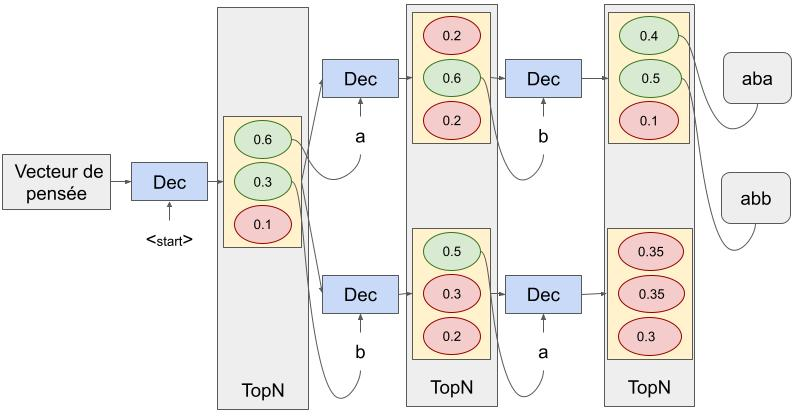
\includegraphics[scale=0.4]{2_production_mots_cles/Beam Search.jpg}
    \caption{Représentation schématique du processus de décodage grâce à l'algorithme de recherche en faisceau.}
    \label{fig:beam_search}
\end{figure}
\todo{refaire en tikz}

\`A l'inverse des algorithmes déterministes que nous avons décrits, notons l'existence des algorithmes d'échantillonnage. Ces algorithmes stochastiques choisissent les mots au hasard en fonction de leur probabilité. Les mots-clés générés par ces algorithmes ne sont donc pas reproductibles, ce qui dans le cadre de la production de mot-clés n'est pas souhaitable. Nous ne considérons donc pas cette technique.

\subsection{Paradigme encodeur-décodeur}\label{sub:paradigme_encodeur_decodeur}

Nous avons présenté dans les sections~\ref{sub:encoding} et \ref{sub:decoding} des moyens d'encoder des documents ainsi que des moyens de générer des séquences.
De nombreuses applications du traitement automatique de la langue nécessitent à la fois l'encodage d'une séquence et son décodage.
Par exemple dans le cadre de la traduction automatique, étant donnée une phrase en langue source, il faut la traduire dans une langue cible, c'est-à-dire qu'il faut encoder la phrase dans la langue source puis générer une phrase correspondante dans la langue cible.
Dans le cadre de la production de mots-clés, il faut générer un mot-clé en fonction d'un document.
Ainsi, le paradigme encodeur-décodeur introduit par \citet{sutskever_sequence_2014}, qui concatène un encodeur et un décodeur, permet de prendre en entrée une séquence de mots de longueur variable et de générer en sortie une autre séquence de mots de longueur variable.
Ce paradigme pallie la limite des réseaux de neurones présentés dans la section~\ref{sub:neural_network} (perceptrons mono ou multicouches) dont l'entrée et la sortie sont de taille fixe.

%Une fois une séquence encodée il est possible de la décoder, c'est-à-dire de produire un mot en fonction d'une représentation $h^t$.
%Générer un mot à partir d'une représentation $h_t$ consiste à passer la représentation dans un perceptron qui calcule une distribution de probabilité sur un vocabulaire, le mot à générer est choisis en fonction de sa probabilité.
    
%\begin{align}
    %\text{log}\: p(y|x) = \sum^m_{j=1} \text{log}\: p(y_j|y_{<j}, x)
%\end{align}

% FROM RECITAL SOTA

\colorlet{enccolor}{green!5}
\colorlet{inputcolor}{black!90!green}
\colorlet{deccolor}{blue!5}
\colorlet{outputcolor}{black!70!blue}
\colorlet{veccolor}{orange!15}
\colorlet{startendcolor}{black!60}
\colorlet{greybox}{black!3}

\begin{figure}[!htb]
\centering

\resizebox{\textwidth}{!}{%
\begin{tikzpicture}

\tikzstyle{cell}=[text centered, rectangle, draw, line width=.5pt, minimum height=1cm, minimum width=1.4cm, rounded corners=2pt]
\tikzstyle{word}=[font=\small\bfseries, text centered, minimum size=.5cm, minimum height=.3cm, text height=1.5ex, text depth=.25ex]
\tikzstyle{vector}=[text centered, rectangle, draw, line width=.5pt, minimum height=.5cm, minimum width=1cm, rounded corners=2pt]
\tikzstyle{arrow}=[shorten >= 2pt, shorten <= 2pt, draw=black!80]

\node[cell, fill=enccolor] (E1) at (0,0){};
\node[cell, fill=enccolor] (E2) at (2,0){};
\node[cell, fill=enccolor] (E3) at (4,0){};
\node[cell, fill=enccolor] (E4) at (6,0){};
\node[text centered] (E5) at (7.5,0){...};
\node[cell, fill=enccolor] (E6) at (9,0){};

\node[word, color=inputcolor, inner color=yellow!50, outer color=white] (I1) at (0,-1.2){Espace};
\node[word, color=inputcolor, inner color=yellow!50, outer color=white] (I2) at (2,-1.2){:};
\node[word, color=inputcolor, inner color=yellow!50, outer color=white] (I3) at (4,-1.2){la};
\node[word, color=inputcolor, inner color=yellow!50, outer color=white] (I4) at (6,-1.2){station};
%\node[word, color=inputcolor, inner color=yellow!50, outer color=white] (I5) at (8,-1.2){...};
\node[word, color=startendcolor] (I6) at (9,-1.2){<fin>};

%\node[cell, fill=veccolor, word, rotate=90] (V) at (11,0){vecteur de pensée};

\node[cell, fill=deccolor] (D1) at (11,0){};
\node[cell, fill=deccolor] (D2) at (13,0){};
\node[cell, fill=deccolor] (D3) at (15,0){};
%\node[cell, fill=deccolor] (D4) at (20,0){};

\node[word, color=startendcolor] (I7) at (11,-1.2){<début>};
\node[word, color=outputcolor, inner color=yellow!50, outer color=white] (O1) at (11,1.2){station};
\node[word, color=outputcolor, inner color=yellow!50, outer color=white] (O2) at (13,1.2){spatiale};
\node[word, color=startendcolor] (O3) at (15,1.2){<fin>};

\draw[->,>=latex,arrow] (E1) -- (E2) node[above,midway] {$h^e_0$};
\draw[->,>=latex,arrow] (E2) -- (E3) node[above,midway] {$h^e_1$};
\draw[->,>=latex,arrow] (E3) -- (E4) node[above,midway] {$h^e_2$};
\draw[->,>=latex,arrow] (E4) -- (E5) node[above,midway] {$h^e_3$};
%\draw[->,>=latex,arrow] (E5) -- (E6) node[above,midway] {$h^e_{n-1}$};
\draw[->,>=latex,arrow] (E5) -- (E6) node[above,midway] {$h^e_{n-1}$};

\draw[->,>=latex,arrow,shorten <= -2pt] (I1) to (E1);
\draw[->,>=latex,arrow,shorten <= -2pt] (I2) to (E2);
\draw[->,>=latex,arrow,shorten <= -2pt] (I3) to (E3);
\draw[->,>=latex,arrow,shorten <= -2pt] (I4) to (E4);
%\draw[->,>=latex,arrow,shorten <= -2pt] (I5) to (E5);
\draw[->,>=latex,arrow,shorten <= -2pt] (I6) to (E6);
\draw[->,>=latex,arrow,shorten <= -2pt] (I7) to (D1);


\draw[->,>=latex, arrow] (E6) -- (D1) node[above,midway] {$h^e_n$};

\draw[->,>=latex,arrow] (D1) -- (D2) node[above,midway] {$h^d_0$};
\draw[->,>=latex,arrow] (D2) -- (D3) node[above,midway] {$h^d_1$};
%\draw[->,>=latex,arrow] (D3) to (D4);

\draw[->,>=latex,arrow,shorten >= -2pt] (D1) to (O1);
\draw[->,>=latex,arrow,shorten >= -2pt] (D2) to (O2);
\draw[->,>=latex,arrow,shorten >= -2pt] (D3) to (O3);
%\draw[->,>=latex,arrow,shorten >= -2pt] (D4) to (O4);

%\node at (5,2) {\large{\textsc{Encodeur}}};
%\node at (17,2) {\large{\textsc{Décodeur}}};

\draw[arrow, rounded corners=3pt] (O1) -| (12, 0);
\draw[->,>=latex, arrow, rounded corners=3pt] (12, 0) -- (12, -1) -| (D2.south);

\draw[arrow, rounded corners=3pt] (O2) -| (14, 0);
\draw[->,>=latex, arrow, rounded corners=3pt] (14, 0) -- (14, -1) -| (D3.south);

%\draw[arrow, rounded corners=3pt] (O3) -| (19, 0);
%\draw[->,>=latex, arrow, rounded corners=3pt] (19, 0) -- (19, -1) -| (D4.south);

\draw[decoration={brace},decorate] (-0.7,1.7) -- node[below=-1.9em] {\large{\textsc{Encodeur}}} (9.7,1.7);
\draw[decoration={brace},decorate] (10.3,1.7) -- node[below=-1.9em] {\large{\textsc{Décodeur}}} (15.7,1.7);


\end{tikzpicture}
}

\caption{Exemple de modèle \textit{encodeur-décodeur} récurrent appliqué à l'extraction automatique de mots-clés.}
\label{fig:seq2seq}
\end{figure}


Le processus d'encodage et de décodage est décrit par l'équation~\ref{eq:enc-dec} et la figure~\ref{fig:seq2seq}.
Dans un premier temps la séquence d'entrée $X$ de taille $n$ est encodée dans le vecteur de pensée $h^e_n$.
Ce vecteur $h^e_n$ est utilisé pour initialiser le premier état caché du décodeur $h^d_0$.
Le décodeur génère ensuite les mots $\hat{y}_t$ qui composent la séquence de sortie $\hat{Y}$ à partir de cet état caché.

\begin{equation}\label{eq:enc-dec}
  \begin{split}
    p(\hat{y}_t | y_{1,...,t-1},h_0) & = \textsc{Softmax}(\sigma(b_v + W_v * h^d_t)) \\
    h^d_t & = \textsc{Rnn}^d(\hat{y}_{t-1}, h^d_{t-1}) \\
    \hat{y}_0 & = \textsc{Debut} \\
    h^d_0 & = h^e_n \\
    h^e_n & = \textsc{Rnn}^e(X) \\
  \end{split}
\end{equation}

Nous présentons ci-après deux améliorations de ce paradigme.
%
D'abord, le mécanisme d'attention qui permet de porter attention à une partie spécifique de l'entrée lors du décodage. Par exemple, la description d'une image nécessite d'identifier les différents objets qui la composent.
%
Ensuite, le mécanisme de copie qui pallie l'incomplétude du vocabulaire de sortie. Ce mécanisme permet au décodeur de copier un mot du document d'entrée au lieu de le générer à partir du vocabulaire de sortie. Le mécanisme de copie est particulièrement utile pour les entités nommées par exemple. Ces entités sont peu fréquentes et ne font généralement pas partie du vocabulaire de sortie.

% Convolution
%Les réseaux de neurones à convolution sont surtout utilisés pour le traitement d'images. Dans le cas du texte, des 
    
% Graphes
%Les réseaux à convolution de graphes (GCN) permettent d'obtenir pour chaque noeud d'un graphe un embedding en fonction de ses voisins. Le nombre de convolutions représente le nombre de bonds qui sont fait entre les noeuds.
    
% Transformer
%Les transformer ont été introduit par \cite{vaswani_attention_2017} et utilisent un mécanisme de self-attention pour chaque mot d'une séquence, de sorte à obtenir pour chaque mot un vecteur qui représente sa relation avec chaque autre mot. Ce mécanisme ne prend pas en compte la séquentialité, en effet chaque calcul est parallélisable. Et ce modèle qui requiert une force de calcul colossale a montré de très bons résultats sur de nombreuse tâches.

\subsubsection{Mécanisme d'attention}
\label{sub:attention_mecanism}

Le mécanisme d'attention~\cite{bahdanau_neural_2014,luong_effective_2015} a été introduit pour améliorer le traitement de longues séquences en permettant au modèle de se focaliser sur certaines parties du document lors du décodage.
%
En effet, un mot-clé concerne seulement certains aspects d'un document. Ce mécanisme permet donc au modèle de porter attention aux parties du document liées à ces aspects.
%
De plus, cette attention au document peut être visualisée grâce aux \emph{poids d'attention} calculés à chaque étape de décodage.
%Par exemple, dans le cadre de la traduction automatique, il permet de visualiser l'alignement entre la phrase en langue source et la phrase en langue cible.
%Par exemple, dans le cadre de la traduction automatique, ce mécanisme permet de visualiser l'importance de chaque mot du document source pour générer la traduction.
La figure~\ref{fig:attention_alignment} illustre cette attention dans le cadre de la traduction automatique pour traduire en français la phrase \say{The agreement on the European Economic Area was signed in August 1992.}
%Il existe généralement un alignement monotone entre les phrases en français et les phrases en anglais.
%Mais ce n'est pas toujours le cas comme le montre le syntagne nominal \say{European Economic Area} dont les mots de la traduction sont dans un ordre inverse \say{zone économique européenne}.
%Le modèle a pu, grâce au mécanisme d'attention, proposer la bonne traduction \say{zone économique européenne} dont l'ordre des mots est inverse à sa traduction.
% Même si le français et l'anglais peuvent généralemnt être traduit mot à mot de manière monotone, le mécanisme d'attention nous permet de visualiser l'alignement non monotone entre zone économique européenne et European Economic Area, en effet l'ordre des noms et adjectifs en français et en anglais est différent.
%Ainsi nous pouvons observer que pour traduire \say{was} en \say{a été}, le modèle à porté attention à \say{was signed} pour comprendre que \say{was} fait parti de la construction du prétérit.
%Pour illustrer ce mécanisme dans le cadre de la traduction automatique nous prenons l'exemple suivant: pour traduire la séquence \say{the European Economic Area} en français (\say{\foreign{la zone économique européenne}}) le modèle portera attention à chaque mot du texte source. Ainsi, pour générer \say{la} et \say{zone} il devra porter attention à \say{\foreign{the}} et \say{\foreign{Area}}. \todo{A revoir.}

\begin{figure}
    \centering
    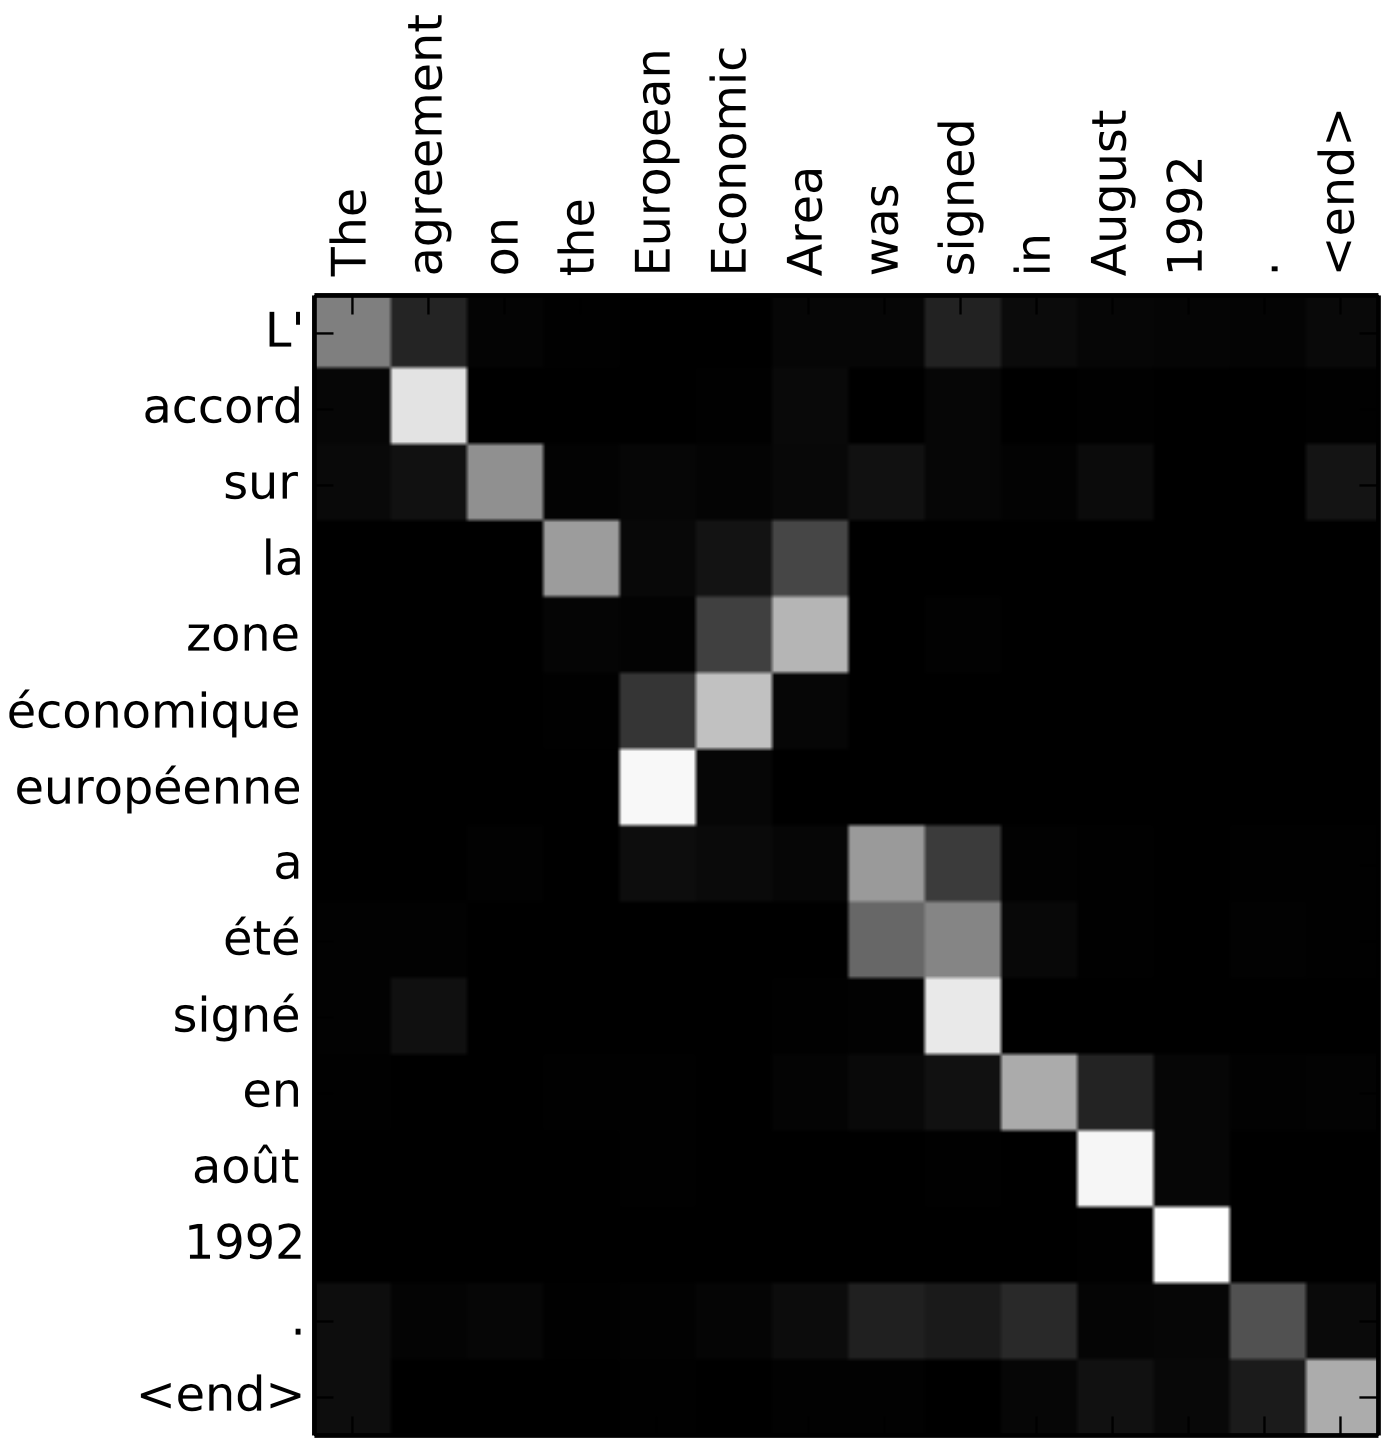
\includegraphics[scale=0.3]{2_production_mots_cles/attention_alignment.png}
    \caption{Exemple de visualisation des poids d'alignement du mécanisme d'attention entre une phrase en anglais et sa traduction en français. Chaque ligne montre la distribution des poids $\alpha_{t}$ ayant servis à générer le mot correspondant en français. Une case blanche indique un poids de 1, une case noire indique un poids de 0. Image extraite de \citet{bahdanau_neural_2014}.}
    \label{fig:attention_alignment}
\end{figure}

%Il faudra aussi porter attention à la syntaxe des deux langues
%Les poids d'attention peuvent être utilisés pour visualiser l'alignement entre les mots de la séquence d'entrée et ceux de la séquence de sortie.
%La figure~\ref{fig:attention_alignment} montre les poids d'alignement dans le cadre de la traduction automatique entre une phrase en anglais et sa traduction en français.

Le décodeur utilise l'état caché courant $h^d_t$ pour générer un mot, le mécanisme d'attention lui permet d'utiliser aussi tous les états cachés de l'encodeur $h^e$ pour mettre à jour l'état caché du décodeur $h^d_t$. Ce mécanisme est décrit dans l'équation~\ref{eq:attention}.
Dans le mécanisme d'attention, les états cachés $h^e$ sont pondérés en fonction de leur importance pour générer le mot $\hat{y}_t$.
Cette importance est établie grâce à une fonction d'alignement $a$ qui calcule une similarité entre l'état caché courant $h^d_t$ et ceux de l'encodeur $h^e$.
Les états cachés $h^e$ sont ainsi moyennés dans le vecteur de contexte $c_t$ utilisé pour mettre à jour l'état caché courant du décodeur $h^d_t$.

Dans l'équation \ref{eq:attention}: $[u;v]$ représente l'opération de concaténation des vecteurs $u$ et $v$; $a$ est une fonction d'alignement qui calcule la similarité entre un état caché de l'encodeur $h^e_t$ et du décodeur $h^d_t$; $\alpha$ représente les poids d'alignement entre les états cachés de l'encodeur $h^e$ et du décodeur $h^d$;  et $\textsc{Softmax}$ est une fonction qui normalise les valeurs d'un vecteur pour qu'il somme à 1.


\iffalse
    \begin{figure}
        \centering
        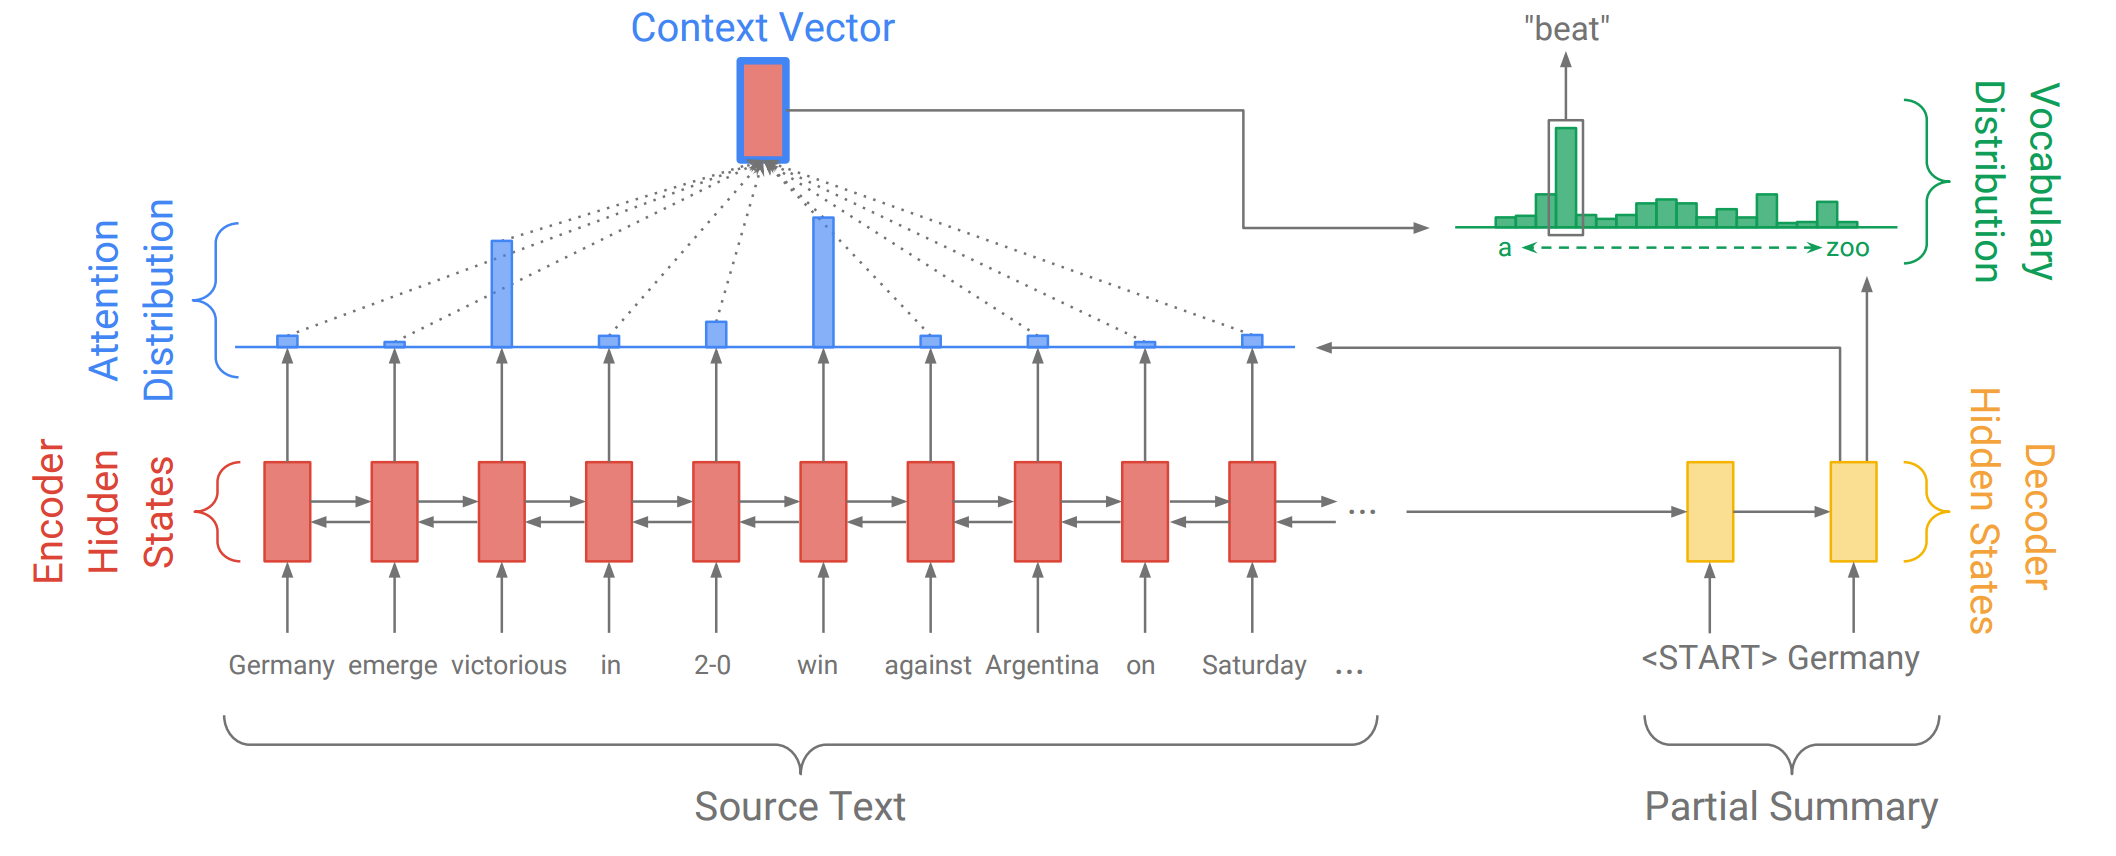
\includegraphics[width=\linewidth]{figures/see_seq2seq-attn.png}
        \caption{Schéma du mécanisme de copie présenté par \cite{see_get_2017}.}
        \label{fig:see_attention}
    \end{figure}
\fi

\begin{equation}\label{eq:attention}
  \begin{split}
    %\hat{Y}_t & = \sigma(b_v + W_v * h^d_t) \\
    p(y_t|y_{<t},x) & = \textsc{Softmax}(\sigma(W_v h^d_t)) \\[.3em]
    h^d_t & = \textsc{Rnn}(y_{t-1}, [h^d_{t-1};c_t]  \\[.3em]
    c_t & = \sum^{|h^e|}_{i=0} \alpha_{i,t} h^e_i \\
    \alpha_{t} & = \textsc{Softmax}(a(h^d_t, h^e)) \\
    %\textsc{Softmax}(x) & = \left[ \frac{x_i}{\sum^{|x|}_{i=0} x_i} , i \in |x| \right]
  \end{split}
\end{equation}

%Le concept d'attention a été présenté de deux manières différentes par \cite{bahdanau_neural_2014} et \cite{luong_effective_2015}.
%
%L'idée de l'attention présentée par~\cite{luong_effective_2015} est \emph{d'utiliser le vecteur de contexte pour prédire $y_t$}.
%
%\cite{bahdanau_neural_2014} présente un autre mécanisme d'attention dont l'idée est de calculer l'état caché du décodeur à l'aide d'un vecteur de contexte. Par rapport à un décodeur classique, seul le calcul de $h^d_t$ change.

\iffalse
    L'idée de l'attention présentée par~\cite{luong_effective_2015} est \emph{d'utiliser le vecteur de contexte pour prédire $y_t$}.
    
    Pour cela, un nouveau $\hat{h}^d_t$ est calculé en fonction d'un vecteur de contexte $c_t$ et de $h^d_t$ (calculé en fonction de $y_{t-1}$ et $h^d_{t-1}$). $c_t$ est la moyenne des $h^e$ pondérés par les scores d'alignement $\alpha$.
    
    Dans leur article, deux manières de calculer l'attention sont présentées: une attention globale et une attention locale.
    %
    Pour l'attention globale, le vecteur de contexte est la moyenne pondérée de toutes les représentations de l'encodeur.
    %
    Pour l'attention locale, le vecteur de contexte est la moyenne pondérée des représentations $h^e$ dans une fenêtre de taille $D$ autour de $h^e_{p_t}$.
    %
    $p_t$ est une valeur entre 0 et $|h^e|$ qui définit le centre de la fenêtre, et peut être calculé de différentes manières.\footnote{Pour plus de détails voir la section 3.2 de \cite{luong_effective_2015}}
    %$p_t$ étant $t$ (dans la traduction automatique on considère que le mot cible $y_t$ est aligné avec le mot source $x_{p_t}$), ou alors un réel entre 0 et $|h^e|$ calculé à l'aide 
    
    \begin{align}
        %y_t & = \sigma(W_v h^d_t) \\
        p(y_t | y_{<t}, x) & = \textsc{Softmax}(W_v \hat{h}^d_t) \\
        \hat{h}^d_t & = \sigma(W_c [c_t;h^d_t]) \\
        c_t & = \sum^{|h^e|}_{i=0} \alpha_{i,t} * h^e_i \\
        \alpha_{i,t} & = \textsc{Softmax}(a(h^e_i, h^d_t)) \\
        h^d_t & = \textsc{Rnn}(y_{t-1}, h^d_{t-1})
    \end{align}
    
    \cite{bahdanau_neural_2014} présente un autre mécanisme d'attention dont l'idée est de calculer l'état caché du décodeur à l'aide d'un vecteur de contexte. Par rapport à un décodeur classique, seul le calcul de $h^d_t$ change. Le calcul du vecteur de contexte est similaire à celui de ~\cite{luong_effective_2015}.
    
    \begin{align}
        p(y_t|y_{<t},x) & = \textsc{Softmax}(W_v h^d_t) \\
        h^d_t & = \textsc{Rnn}(y_{t-1}, [h^d_{t-1};c_t]  \\
        c_t & = \sum^{|h^e|}_{i=0} \alpha_{i,t} * h^e_i \\
        \alpha_{i,t} & = \textsc{Softmax}(a(h^e_i, h^d_t))
    \end{align}
    
    Il existe différentes fonctions d'alignement:
    
    bahdanau $a(h^e_i, h^d_t) = v_a \text{tanh}(W_a h^d_t + U_a h^e_i)$
    
    dot $a(h^e_i, h^d_t) = h^e_i h^d_t$
    
    general $a(h^e_i, h^d_t) = h^e_i W_a h^d_t$
    
    concat $a(h^e_i, h^d_t) = W_a [h^e_i;h^d_t]$
\fi

\subsubsection{Mécanisme de copie}
\label{sub:copy_mecanism}

Le mécanisme de copie~\cite{see_get_2017,gu_incorporating_2016} provient des tâches de traduction automatique et de résumé automatique. Il a pour but de produire des mots peu fréquents ou hors du vocabulaire de sortie.
En effet, les modèles neuronaux qui génèrent du texte choisissent les mots dans un vocabulaire de sortie comportant généralement \num{50 000} mots.
Dans les tâches sus-citées, les mots peu fréquents qui ne font pas partie du vocabulaire de sortie, comme les entités nommées ou les transfuges, doivent pourtant apparaître dans la séquence de sortie.
%Le mécanisme de copie ~\cite{see_get_2017,gu_incorporating_2016} pallie ce problème en permettant au décodeur de générer un mot du vocabulaire de sortie ou bien de copier un mot du document.
Deux mécanismes de copie ont été proposés par \citet{see_get_2017} et \citet{gu_incorporating_2016}; les deux étant similaires, nous présentons ici le premier car plus simple. Il est décrit dans l'équation~\ref{eq:copy_mecanism}.

% exemple
%Le mécanisme d'attention a été utilisé comme post-traitement pour remplacer les mots inconnus de la sortie par les mots de l'entrée alignés par le mécanisme d'attention. Ceci permettant de traiter les entités nommées peu fréquentes ou les transfuges.
%
%Le mécanisme de copie vient automatiser ce processus en permettant au modèle de générer un mot du vocabulaire ou de copier un mot du document.

%, tous deux inspirés des réseaux de pointeurs~\cite{vinyals_pointer_2015} qui génèrent une séquence de pointeurs vers la séquence d'entrée.
Ce mécanisme utilise le vocabulaire de la séquence d'entrée $\mathcal{X}$ (particulier à chaque document) en plus du vocabulaire de sortie $\mathcal{V}$.
Pour produire un mot, une distribution de probabilité sur le vocabulaire  $P_{vocab}(y_{t})$ est calculée comme précédemment par le décodeur (cf. section~\ref{sub:decoding}) et les poids du mécanisme d'attention $\alpha$ (cf. section~\ref{sub:attention_mecanism}) sont utilisés pour estimer la probabilité de copie de chaque mot du document.
Les poids d'attention $\alpha$ des mots qui apparaissent plusieurs fois dans l'entrée $x$ sont sommés $\sum_{j,x_j=y_{t,i}} \alpha^t_j$.
Ainsi, un mot peut être généré à partir du vocabulaire de sortie $\mathcal{V}$ ou copié à partir du vocabulaire du document $\mathcal{X}$.
Les probabilités de copie et de génération d'un même mot, qui appartient au document et au vocabulaire, sont sommées.
Dans l'équation~\ref{eq:copy_mecanism}: $h^d_t$, $c_t$ et $\alpha^t_j$ proviennent du mécanisme d'attention (cf. équation~\ref{eq:attention}); $p_{gen}$ est un curseur permettant au modèle de privilégier la copie ou la génération et $P_{vocab}(y_t)$ est une distribution de probabilité sur le vocabulaire de sortie $\mathcal{V}$.

%Les probabilités de génération et de copie sont combinés pour donner une distribution de probabilités sur $\mathcal{X} \cup \mathcal{V}$.

\begin{equation}\label{eq:copy_mecanism}
  \begin{split}
    p(y_{t,i}|y_{<t},x) & = p_{gen} P_{vocab}(y_{t,i}) + (1 - p_{gen}) \sum_{j,x_j=y_{t,i}} \alpha^t_j \\
    p_{gen} & = \sigma(W_h h^d_t + W_c c_t + W_y y_{t-1}) \\
    P_{vocab}(y_{t}) & = \textsc{Softmax}(\sigma(W_v h^d_t))
  \end{split}
\end{equation}

%ou les poids d'un mécanisme d'attention supplémentaire, utilisé seulement pour calculer le score de copie, pour~\cite{gu_incorporating_2016}

\iffalse
    %\cite{gu_incorporating_2016}, création d'un vocabulaire spécifique a chaque instance, composé de $\mathcal{V}$ le vocabulaire normal et $\mathcal{X}$ le vocabulaire des mots de l'entrée.
    %
    %Ça change le calcul de $y_t$ par rapport au mécanisme d'attention.
    %
    %On défini les vecteurs $\psi_g \in \mathds{R}^|\mathcal{V}|$ et $\psi_c \in \mathds{R}^|\mathcal{X}|$ qui contiennent respectivement les score de copie et de génération.
    
    % attentive read = les poids de l'attention
    % selective read = les poids de l'"attention" du mécanisme de copie
    
    \begin{align}
        y_t & = \textsc{Softmax}(e^{P_{gen}} +e^{P_{copy}}) \\
        P_{gen} & = W_v h^d_t \\
        P_{copy} & = \left[ \sum^{|h^e|}_{j=0, x_j=x_i} \sigma(h^e_j W_c) h^d_t | x_i \in \mathcal{X} \right] \\
        h^d_t & = RNN([y_{t-1};cc_t)],h^d_{t-1}) \\
        cc_t & = \sum^{|h^e|}_{i=1} aa_{t,i} h^e_t \\
        aa_{t,i} & = \textsc{Softmax}()
    \end{align}
    
    %\cite{see_get_2017} reprend le mécanisme d'attention de \cite{luong_effective_2015} et modifie le calcul de $y_t$ en ajoutant une probabilité de copie et un curseur privilégiant la copie ou la génération.
    
    \begin{align}
        p(y_{t,i}) = p_{gen} P_{vocab}(y_{t,i}) + (1 - p_{gen}) \sum_{j,x_j=y_{t,i}} \alpha^t_j \\
        p_{gen} = \sigma(W_c c_t + W_h h^d_t + W_y y_{t-1})
    \end{align}
\fi

% Multitache
% Conditional Random Field
% Reinforcement Learning : adaptative reward


\section{Méthodes de bout-en-bout}
\label{methodes-de-bout-en-bout}

\todo{Ajouter des schéma pour mieux comprendre les méthodes.}

Dans cette section nous présentons un état de l'art des méthodes de bout-en-bout.
Ces méthodes, contrairement aux méthodes en chaîne de traitement (cf. section~\ref{sec:methode-en-chaine-de-traitement}), prennent en entrée un document et laissent le soin au modèle d'en extraire les caractéristiques pour retourner un ensemble de mots-clés sans étapes intermédiaires ni définition manuelle de ces caractéristiques.
Parmi les méthodes proposées dans la littérature, nous distinguons les méthodes génératives, qui peuvent produire des mots-clés présents et des mots-clés absents, des méthodes extractives, limitées aux mots-clés présents.

Jusqu'à présent, toutes les méthodes de bout-en-bout qui ont été proposées sont supervisées et reposent sur des réseaux de neurones (cf. section~\ref{sub:neural_network}) qui nécessitent de grandes quantités de données annotées pour être entraînées.
%
Le développement de ces méthodes démarre avec l'introduction du jeu de données KP20k et de la méthode générative CopyRNN par \citet{meng_deep_2017}.
Le jeu de données KP20k, qui comporte $\simeq$\num{550000} documents, comble un manque.
En effet, seuls de petits jeux de données (de l'ordre du millier de documents) étaient jusqu'alors disponibles.
Ce travail a ainsi lancé une nouvelle direction de recherche sur les méthodes génératives de production de mot-clés.

\begin{figure}
    \centering
    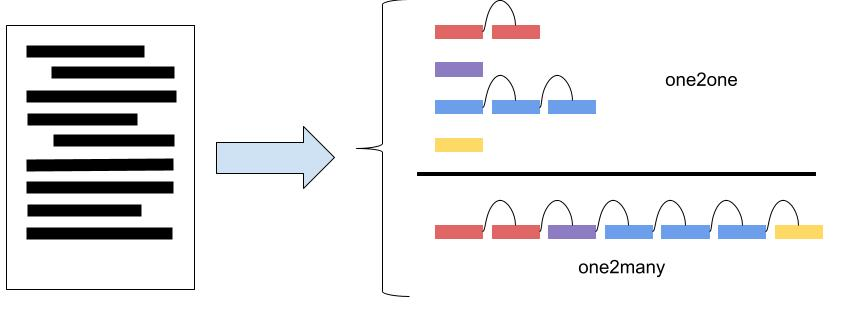
\includegraphics[scale=0.4]{2_production_mots_cles/Decoding strategies.jpg}
    \caption{Représentation schématique des stratégies de décodage \emph{one2one} et \emph{one2many}.}
    \label{fig:decoding_strategies}
\end{figure}
\todo{Refaire en tikz}

Dans cet état de l'art, nous présentons tout d'abord les méthodes automatiques de génération de mots-clés de bout-en-bout, qui sont au c\oe{}ur de ce travail de thèse.
Nous présentons ces méthodes de génération en deux parties: premièrement, les méthodes qui générent les mots-clés un à un (\emph{one2one}), et deuxièmement, celles qui génèrent des séquences de mots-clés (\emph{one2many}). Ces deux types de génération sont schématisés dans la figure~\ref{fig:decoding_strategies}.
Nous présentons ensuite les méthodes extractives de bout-en-bout, c'est-à-dire celles qui se limitent aux seuls mots-clés présents.

\subsection{Génération de mots-clés}
\label{sub:generation_de_mots_cles}

Les méthodes génératives, introduites par \citet{meng_deep_2017}, ont pour objectif de pallier deux faiblesses qui concernent la majorité des méthodes extractives présentées précédemment: l'impossibilité de produire des mots-clés absents ainsi que la faible prise en compte de la sémantique.
Le paradigme encodeur-décodeur sur lequel les méthodes génératives sont fondées permet d'encoder la sémantique du document.
Ainsi, les mots-clés produits sont le fruit d'une \say{compréhension} du document, contrairement aux méthodes en chaîne de traitement qui s'intéressent à l'\say{importance} des mots dans le document indépendamment de leur sens.
%
Ces méthodes génératives rendent possible la production de mots-clés absents grâce à la manière dont le décodeur génère la séquence de sortie.
Ce processus s'effectue en choisissant, à chaque étape de décodage, un mot à partir d'un vocabulaire de sortie qui est plus grand et différent du vocabulaire du document.
Ces méthodes génératives apprennent à générer des mots-clés un par un (génération \emph{one2one}, voir figure~\ref{fig:decoding_strategies}), c'est-à-dire que chaque document $X$ et son ensemble de mot-clés $Y$ de taille $N$ forment un couple $(X, \{Y_0, ..., Y_N\})$, décomposé en autant d'exemples d'entraînement que de mots-clés, $(X, Y_0), ... , (X, Y_N)$.

%\paragraph{Définitions}
%\todo{Il faudrait définir avant les principaux modèles: one2one, séquence avant de les définir formellement; Fait ausi des dessins}
%$x$ et $y$ représentent des mots, $p$ des mots-clés. Étant donné un ensemble de données $D = {(x^i,p^i), i \in 1...N}$ de taille $N$, un exemple est composé d'un document $x^i$ et d'un ensemble de mots-clés $p^i = {p^i_j, j \in 1...M^i}$ de taille $M^i$. Les documents et les mots-clés sont composés de mots $[x^i_k, k \in 1...N^i]$ et $[y^i_j]$ est composé d'un document composé d'une séquence de mots $x^i = (x^i_1, ..., x^i_{N^i})$ de longueur $N^i$ et d'un ensemble de mots-clés $p^i$ de taille $M^i$ avec $p^i = (p^i_1, ..., p^i_{M^i})$, où chaque mot-clé est une séquence de mots de taille $M^{i,j}$ avec $p^{i,j} = (y^{i,j}_1, ..., y^{i,j}_{M^{i,j}})$. Dans le cadre des modèles one2one, un couple document -- mots-clés est découpé en $M^i$ différents couples $(x^i, p^{i,1}), ..., (x^i, p^{i, M^i})$. 
%Pour les modèles en séquences, les mots-clés sont concaténés de sorte à former une unique séquence $(x^i, y^{i,1}_1 \lozenge ... \lozenge y^{i,1}_{M^{i,j}} \lozenge \text{SEP} \lozenge y^{i,2}_1 \lozenge ... \lozenge y^{i,M^i}_{M^{i,j}})$.

La méthode pionnière de génération automatique de mots-clés appliquée aux documents scientifiques est CopyRNN~\cite{meng_deep_2017}.
%
L'architecture neuronale de cette méthode s'inspire du processus d'annotation humain qui consiste à lire le document pour le comprendre dans son entièreté puis à le résumer grâce à des mots-clés.
%Aussi, les humains peuvent facilement s'abstraire du texte et faire appel à leurs connaissances pour produire des mots-clés qui n'apparaissent pas dans le texte.
Pour reproduire ce processus, CopyRNN utilise le paradigme encodeur-décodeur, que nous avons présenté dans la section~\ref{sub:paradigme_encodeur_decodeur}, pour encoder un document et le décoder ensuite en un mot-clé. % Ainsi un réseau de neurones récurrent encode le document dans un vecteur de pensée, puis un autre décode, génère, ce vecteur de pensée en un mot-clé.
Pour améliorer les performances des modèles encodeur-décodeur, il est commun d'utiliser un mécanisme d'attention (voir section~\ref{sub:attention_mecanism}).
Ce mécanisme permet au modèle de porter attention à certaines parties du document lors de la génération d'un mot.
%
Un mécanisme de copie est aussi ajouté au modèle pour lui permettre de générer des mots peu fréquents (voir section~\ref{sub:copy_mecanism}).
Ce mécanisme de copie modifie le décodage en permettant de générer un mot à partir du vocabulaire de sortie ou bien à partir du document.\\
%
Cette méthode obtient des performances bien plus élevées que les précédentes méthodes extractives. Les performances de CopyRNN sont de l'ordre de 30 points de \fmesure{} pour les mots-clés présents tandis que les performances des méthodes extractives sont généralement en dessous de 20 points de \fmesure{}.
Les mots-clés absents, qui ne pouvaient jusque-là pas être produits, correspondent peu à la référence: parmi les 50 meilleurs mots-clés absents un seul apparaît dans la référence.


%La communauté scientifique présente de nouvelles méthodes basées sur CopyRNN et tente de l'améliorer.
% les méthodes essaient de résoudre les problèmes identifiés
%Les méthodes présentées augmentent toujours les performances de génération des mots-clés présents et absents.

Certaines méthodes proposées essaient d'améliorer l'encodage du document.
\citet{chen_title-guided_2019}, par exemple, constate que les mots-clés ne sont pas uniformément distribués dans les documents.
En particulier \npercent{60} des mots-clés de référence ont au moins un mot en commun avec le titre du document.
Pour prendre cela en compte, ils proposent TGNet (Title Guided Network), qui étend CopyRNN en introduisant un nouvel encodeur spécifique au titre, en plus de l'encodeur du document.
Cet encodage du titre permet de donner un poids supplémentaire à l'information qu'il contient.
Ces deux représentations (du titre et du document) sont ensuite combinées puis fournies au décodeur.
Cette méthode améliore nettement les performances de génération des mots-clés présents et absents par rapport à CopyRNN (+\npercent{5} sur KP20k).
% Ils ne regardent que la F-mesure présent/absent rien d'autre

La redondance dans les ensembles de mots-clés produits est un problème récurrent dans les méthodes de production de mots-clés.
En effet, \citet{hasan_automatic_2014} montrent que 8 à \npercent{12} des erreurs des méthodes sont liées à la redondance des mots-clés.
Ainsi, les méthodes en chaîne de traitement mettent en place des stratégies, notamment lors de la sélection du sous-ensemble de mots-clés, pour limiter cette redondance (voir section~\ref{choisir-le-sous-ensemble}).
Dans cette ligne de recherche, \citet{zhao_incorporating_2019} remarquent les méthodes de bout-en-bout ne sont pas exemptes de ce problème, ils s'intéressent ainsi au chevauchement entre les mots-clés générés et ceux de référence.
Par exemple, \npercent{23.98} des mots-clés unigrammes générés par CopyRNN font partie d'un mot-clé de référence, et \npercent{47.15} des mots-clés 4-grammes générés par CopyRNN contiennent un mot-clé de référence.
Dans l'optique de limiter ces chevauchement, ils présentent le modèle ParaNet$_T$+CoAtt qui entraîne le modèle, à générer à la fois les mots-clés et leurs étiquettes morphosyntaxiques, ainsi la syntaxe des mots-clés générés sera similaire à celle des mots-clés de référence.
Pour cela ils ajoutent au modèle CopyRNN un encodeur, pour les étiquettes morphosyntaxiques des mots du document, ainsi qu'un décodeur, pour celles du mot-clé.\footnote{Les étiquettes morphosyntaxiques du document et des mots-clés proviennent de l'outils Stanford CoreNLP.}
Les informations des deux décodeurs sont ensuite combinées et utilisées pour générer les mots-clés et leurs étiquettes morphosyntaxiques.
%Grâce à cette méthode, les mots-clés générés chevauchent moins les mots-clés de référence; par exemple le pourcentage de mot-clés 4-grammes contenant un mot-clé de référence a baissé de \npercent{10}.

\begin{figure}
    \centering
    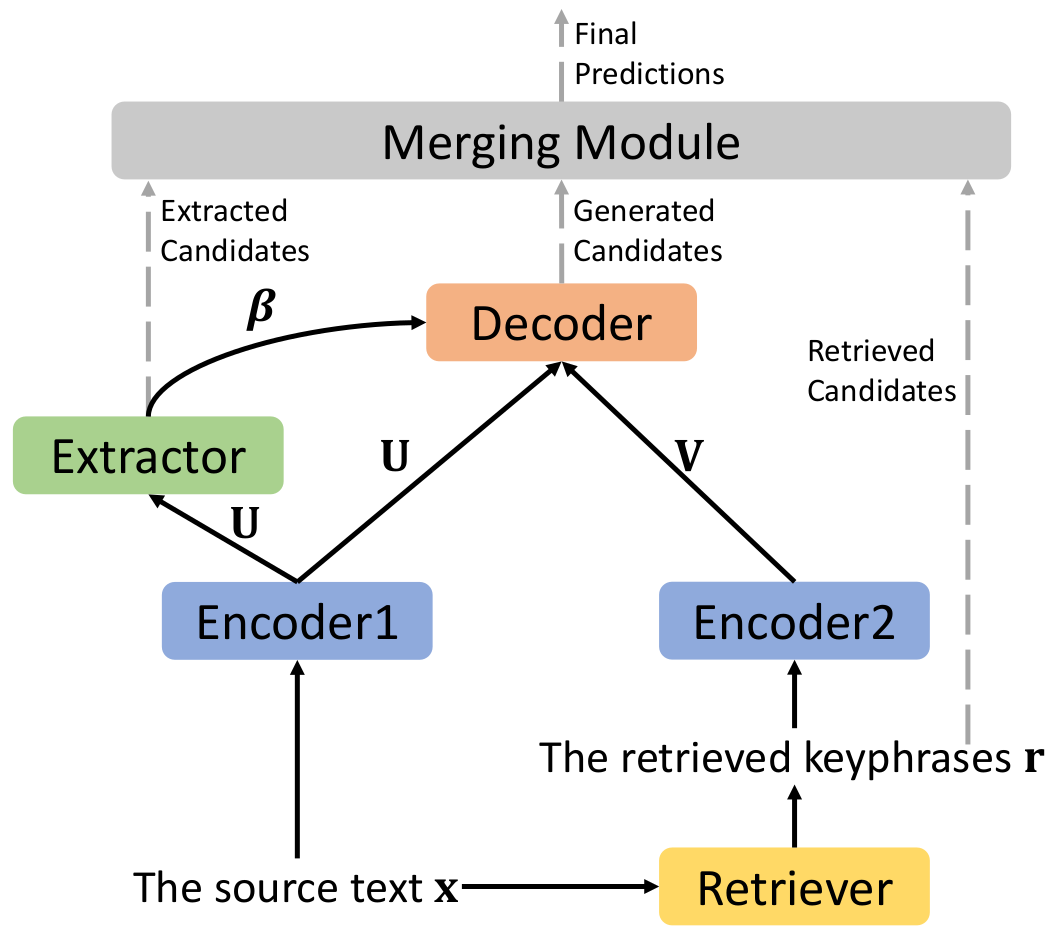
\includegraphics[scale=0.2]{2_production_mots_cles/kg_ke_kr_m.png}
    \caption{Représentation schématique de l'architecture de la méthode KG-KE-KR-M. Image extraite de~\citet{chen_integrated_2019}.}
    \label{fig:schema_kgkekrm}
\end{figure}

%Le processus manuel d'annotation en mots-clés est composé de plusieurs étapes: la lecture du document, l'extraction des mots-clés dans le document puis l'attribution de mots-clés absents du document et enfin la combinaison des mots-clés provenant de ces deux processus d'annotation.
Dans l'optique de reproduire l'annotation humaine, \citet{chen_integrated_2019} propose la méthode KG-KE-KR-M qui produit un ensemble de mots-clés en combinant différentes méthodes: génération de mots-clés, extraction de mots-clés, récupération de mots-clés (voir figure~\ref{fig:schema_kgkekrm}).
%Ces différentes méthodes sont entraînées de bout-en-bout puis les mots-clés de chaque méthode sont pondérés grâce à un classifieur.
%
Dans un premier temps, cette méthode récupère les mots-clés de référence des $K$ documents d'entraînement les plus proches du document traité (grâce à la distance de Jaccard).
Ces mots-clés \emph{récupérés} sont concaténés puis encodés. Ils serviront à conditionner la génération de mots-clés.
Dans un second temps, des mots-clés sont \emph{extraits} du document en classifiant chaque mot comme mot-clé ou non mot-clé.
%Cette classification s'effectue grâce aux états cachés du document encodé.
Ensuite, des mots-clés sont \emph{générés} à partir du document ainsi que des mots-clés récupérés et des mots-clés extraits.
Enfin, les mots-clés récupérés, extraits et générés sont pondérés grâce à un classifieur.
Cette méthode à la particularité de combiner les méthodes en chaîne de traitement (sélection de candidats puis pondération) et les méthodes de bout-en-bout (apprentissage conjoint de la génération et de l'extraction).
Malgré la grande diversité dans les techniques de production de mots-clés candidats, les performances ne sont pas significativement supérieures à CopyRNN. Cette méthode produit néanmoins plus de mots-clés absents de référence que CopyRNN.

La méthode CorrRNN~\cite{chen_keyphrase_2018} considère que les mots-clés doivent couvrir l'ensemble des sujets du document et être divers, c'est-à-dire que chaque mot-clé doit concerner un sujet différent.
Cette méthode étend CopyRNN en y ajoutant un mécanisme de couverture et un mécanisme de revue.
Le mécanisme de couverture encourage le modèle à porter attention aux différentes parties du document.
Il conserve et accumule les scores d'attention des mots du document à chaque étape de décodage, et il est inclus dans le calcul du mécanisme d'attention.
Ensuite, le mécanisme de revue est essentiellement un mécanisme d'attention sur les mots générés.
Son objectif est d'identifier les sujets déjà couverts par les mots-clés générés et ainsi de générer des mots-clés qui concernent des sujets non traités.
Cette méthode est la première à prendre en compte les mots-clés déjà générés dans le processus de génération, pour cela la phase d'entraînement est modifiée.
Au lieu de rétro-propager le gradient après chaque mot-clé de référence, la phase de rétro-propagation n'est effectuée qu'une fois tous les mots-clés de référence du document traités.
%Chaque mot-clé est généré en utilisant les mécanismes de couverture et de redondance, qui prennent en compte les mots-clés déjà générés; le gradient est ensuite calculé grâce à l'erreur de chaque mot-clé; et enfin, rétro-propagé.
%Cette méthode améliore les performance de production de mots-clés présent par rapport à CopyRNN, mais l'article ne présentant pas ses résultats sur le jeu de données de référence KP20k et utilisant des métriques peu utilisés dans les autres travaux la comparaison est limitée.

\subsection{Génération de séquences de mots-clés}% (\textsc{One2Seq})}
%\subsection{Génération en séquence}
\label{sub:generation_de_sequences_de_mots_cles}

%Nous avons présenté dans la section précédente, des méthodes génératives qui apprennent à générer un mot-clé par document.
Nous présentons dans cette section des méthodes qui apprennent à générer des séquences de mots-clés (génération \emph{one2many}, voir figure~\ref{fig:decoding_strategies}). C'est-à-dire que chaque exemple d'entraînement est composé d'un document et de la concaténation des mots-clés de référence en une unique séquence dans laquelle ils sont séparés par un symbole de séparation. Par exemple, l'ensemble de mots-clés $\{$ Classe , Fichier log , Agrégat $\}$ sera transformé en \say{Classe \texttt{SEP} Fichier log \texttt{SEP} Agrégat \texttt{FIN}}.
%Le développement des méthodes utilisant la génération \emph{one2many} part du constat que la génération \emph{one2one} ne permet pas de prendre en compte les mots-clés déjà générés et que les ensembles de mots-clés sont souvent redondants~\cite{hasan_automatic_2014}.
Le développement des méthodes génératives \emph{one2many} part du constat que les ensembles de mots-clés produits sont souvent redondants~\cite{hasan_automatic_2014} et que la génération \emph{one2one} ne permet pas de pallier ce problème.
En effet, les méthodes \emph{one2many} font l'hypothèse qu'avec la génération en séquence, le modèle ayant accès aux mots-clés déjà générés, il ne générera pas de mots-clés redondants.
%
Cette méthode de génération permet au modèle de générer le même nombre de mots-clés que la référence, en effet, il apprend en même temps qu'à générer les mots-clés, à placer les séparateurs de mots-clés et le symbole de fin.
Ainsi, ces méthodes peuvent générer des mots-clés selon deux stratégies~\cite{yuan_one_2020}: l'\textbf{inférence exhaustive} qui utilise l'algorithme de recherche en faisceau pour sur-générer des mots-clés et ainsi en obtenir un nombre fixe pour chaque document, c'est la stratégie employée par les méthodes génératives \emph{one2one}; et l'\textbf{inférence auto-régulée} (\foreign{self-terminating}) dans laquelle le décodage s'arrête lors de la génération du symbole de fin, cette stratégie permet au modèle de produire un nombre pertinent de mots-clés pour le document.
La seconde stratégie de décodage permet donc de s'affranchir du choix arbitraire du nombre de mots-clés $n$ à produire (voir section~\ref{choisir-le-sous-ensemble}).

Pour entraîner ces modèles, les mots-clés sont concaténés, mais ce processus n'est pas trivial.
En effet, l'ordre dans lequel les mots-clés sont concaténés influence les performances des modèles.
L'étude de \citet{meng_empirical_2021} compare différentes manières d'ordonner les mots-clés, telles que: \emph{No-Sort} qui laisse l'ordre par défaut; \emph{Alpha} qui trie par ordre alphabétique; \emph{Pres-Abs} qui place les mots-clés présents avant les mots-clés absents. L'étude montre que c'est l'ordre \emph{Pres-Abs} qui donne les meilleures performances.

La première méthode à générer des séquences de mots-clés est catSeqD~\cite{yuan_one_2020,yuan_generating_2018}.
L'objectif de cette méthode, similaire à CorrRNN, est d'augmenter la diversité des mots-clés générés.
%
Pour cela, le modèle CopyRNN, utilisé comme base, est augmenté d'un mécanisme de couverture sémantique et de régularisation orthogonale pour former le modèle catSeqD.
%
Le mécanisme de \emph{couverture sémantique} repose sur l'hypothèse que l'ensemble de mots-clés de référence et le document encodent la même information.
Ainsi, un nouvel encodeur est entraîné à encoder les mots-clés et à produire la même représentation que pour le document.
Il encode la séquence au fur et à mesure de sa génération et l'état cachés qui en résulte conditionne la prédiction du mot suivant, cela contraint les mots-clés générés à être proche sémantiquement du document.
%
Ensuite, les auteurs constatent que les mots générés après les séparateurs de mots-clés sont souvent similaires.
Le mécanisme de \emph{régularisation orthogonale} pallie ce problème en diversifiant explicitement les représentations des séparateurs, en pénalisant, dans la fonction de coût, ces représentations si elles ne sont pas orthogonales.

\todo{Refaire en Tikz}
\begin{figure}
    \centering
    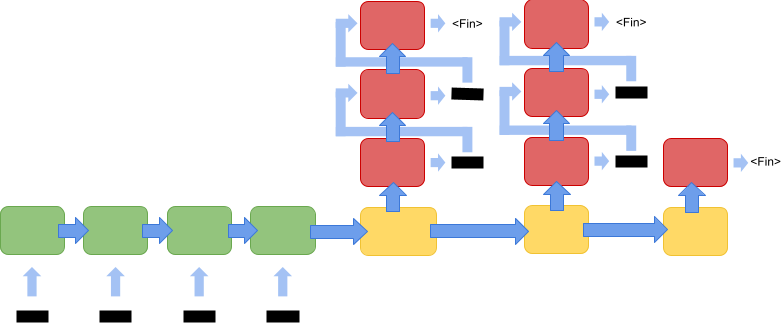
\includegraphics[scale=0.5]{2_production_mots_cles/exhird.png}
    \caption{Représentation schématique du décodage hiérarchique de la méthode ExHirD. L'encodeur du document est représenté en vert, le décodeur de concept en jaune et le décodeur de mots-clés en rouge.}
    \label{fig:schema_exhird}
\end{figure}

Dans le but de mieux modéliser les ensembles de mots-clés, \citet{chen_exclusive_2020} s'intéressent à la structure hiérarchique des ensembles de mots-clés.
En effet, les méthodes de génération de séquences de mots-clés identifient les mots-clés grâce à des marqueurs générés par le modèle. Cette séquentialité ne permet pas de représenter la hiérarchie entre les mots-clés et les mots qui les composent.
Ces travaux se rapprochent de \citet{yuan_generating_2018} qui essaient de rompre la séquentialité en modifiant la représentation des séparateurs de mots-clés avec le mécanisme de régularisation orthogonale.
Ainsi, ils présentent la méthode ExHirD~\cite{chen_exclusive_2020} dans laquelle le décodeur de l'architecture de CopyRNN est remplacé par un décodeur hiérarchique (voir figure~\ref{fig:schema_exhird}) qui génère les mots-clés en deux temps: d'abord l'identification des concepts, ensuite la génération de leur représentation textuelle.
Ce décodeur hiérarchique comprend un premier décodeur qui produit une représentation dense d'un concept, puis un second décodeur qui va générer une séquence de mots à partir de cette représentation dense pour instancier le concept en un mot-clé.
La génération des mots utilise deux mécanismes d'attention sur les documents d'entrée: l'un est conditionné par la représentation dense du concept; l'autre, standard, est conditionné par le mot précédent.
Ainsi, ce décodeur hiérarchique permet de modéliser explicitement les concepts importants du document et les mots qui les décrivent.
%
L'évaluation de cette méthode montre néanmoins un faible gain de performance, de l'ordre d'un point de F@5, pour les mots-clés présents et absents.
%
Ces travaux s'attellent aussi au problème de redondance des mots-clés et proposent un mécanisme de décodage exclusif pour tenter de le résoudre.
Ce mécanisme, simple dans son idée, interdit au modèle de générer deux mots-clés commençant par le même mot.
En effet, les mots-clés comportent le plus souvent entre 1 et 4 mots (voir section~\ref{sub:nature_linguistique}), ainsi le premier mot affecte grandement les suivants.
Ce mécanisme n'est pas limité à la méthode ExHirD; il peut être adapté aux différents types de décodage ou être utilisé en post-traitement.
Son évaluation montre qu'il fait significativement baisser le nombre de mots-clés dupliqués sans faire baisser les scores de F@5.

Les méthodes génératives \emph{one2many} apprennent à déterminer le nombre de mots-clés à produire mais en génèrent trop peu: catSeqD génère en moyenne 4,3 mots-clés par document alors que la référence en est composée de 5,3 en moyenne.
Les travaux de \citet{chan_neural_2019} s'intéressent à encourager les modèles à générer plus de mots-clés, en les entraînant à optimiser le rappel et la \fmesure{}.
Or ces métriques ne peuvent être utilisées comme fonction de coût dans l'algorithme de descente de gradient, car elles ne sont pas dérivables.
Pour résoudre ce problème, les auteurs proposent d'utiliser l'apprentissage par renforcement pour affiner\footnote{\foreign{To fine-tune} en anglais.} des modèles déjà entraînés.
%
Dans l'apprentissage par renforcement~\cite{williams_simple_1992}, un agent produit une série d'actions en suivant une politique (ici la génération de mots grâce à un modèle génératif), puis est récompensé pour chacune des actions.
%Dans l'apprentissage par renforcement~\cite{williams_simple_1992}, un agent produit une série d'actions en suivant une politique puis il est récompensé pour chaque action.
%Dans notre cas, une action consiste à générer un mot, la politique permettant de choisir le mot est un modèle génératif, et la récompense est le rappel ou la f-mesure.
L'algorithme d'apprentissage par renforcement optimise ainsi les poids du modèle (met à jour la politique) en fonction de la récompense.
%
Dans la méthode proposée, la récompense s'adapte selon le nombre de mots-clés générés: s'il est trop faible, la récompense sera le rappel pour encourager le modèle à générer plus de mots-clés; à l'inverse s'il est trop grand, la récompense sera la \fmesure{}, pour encourager le modèle à générer seulement de bons mots-clés.
%
De plus, les mots-clés présents et absents sont récompensés séparément pour favoriser la génération des mots-clés absents.

%CDKGen~\cite{diao_keyphrase_2020} (use close docs to encode, transformers)
%SenseNet~\cite{luo_sensenet_2020} (??)

Les travaux, concernant les méthodes neuronales, présentés jusqu'à présent considèrent que la quantité de données disponibles est suffisante.
Nous verrons dans le chapitre~\ref{chap:framework} que les sources de données contenant des documents annotés en mots-clés sont peu nombreuses malgré la large disponibilité de documents scientifiques en ligne.
Ainsi, les travaux de \citet{ye_semi-supervised_2018} se placent dans un cadre où la quantité de documents annotés est limitée.
%
Pour cela, les auteurs proposent deux méthodes qui tirent parti de la masse de documents non annotés pour la génération de mots-clés.
%
La première méthode consiste à utiliser des documents non annotés en mots-clés dans le cadre d'apprentissage multitâche.
Un réseau de neurones encodeur-décodeur est entraîné, pour les documents annotés, à générer des séquences de mots-clés et, pour les documents non annotés, à générer le titre du document. Dans le modèle, deux décodeurs différents sont utilisés pour chacune des tâches mais l'encodeur est partagé.
%
La seconde méthode consiste à créer un corpus synthétique en annotant automatiquement des documents en mots-clés. Les mots-clés sont extraits grâce aux méthodes \tfidf{} et TextRank.
Ainsi, un modèle de génération de mots-clés est pré-entraîné grâce à la combinaison des corpus synthétique et annoté, puis affiné grâce au seul corpus annoté.
%
L'évaluation des deux modèles résultant de ces méthodes d'entraînement montre qu'ils obtiennent des résultats similaires.
Les scores de F@5 pour les mots-clés présents des modèles semi-supervisés sont comparables à ceux du modèle \emph{catSeq} (CopyRNN entraîné à générer des séquences de mots-clés), bien qu'ils n'utilisent qu'un dixième des documents annotés utilisés par \emph{catSeq}.

\subsection{Extraction de mots-clés}

% Chapeau
Les méthodes génératives de bout-en-bout sont très performantes pour produire des mots-clés présents, mais génèrent très peu de mots-clés absents.
Ainsi, la communauté scientifique s'intéresse à des méthodes de bout-en-bout exclusivement extractives.
%Les méthodes génératives de bout-en-bout sont très performantes pour produire des mots-clés présents, ainsi la communauté scientifique s'intéresse à 
%Les méthodes génératives de bout-en-bout, qui ont la particularité de produire des mots-clés absents, n'en produisent au final que très peu~\cite[inter alia]{chen_exclusive_2020, santosh_hicova_2021} et ceux-ci ne correspondent que très peu aux mots-clés de référence~\cite[inter alia]{ahmad_select_2020, ye_one2set_2021}.
%Mais leurs performances élevées pour produire des mots-clés présents encouragent tout de même le développement de méthodes de bout-en-bout.
%C'est pourquoi la communauté scientifique s'intéresse aux méthodes de bout-en-bout exclusivement extractives.
%
Bien qu'elles ne soient pas au c\oe{}ur de nos travaux, nous présentons les principales méthodes extractives par soucis d'exhaustivité.
% Plan
Dans cette section nous présentons tout d'abord les méthodes fondées sur l'annotation en séquence, ensuite, une méthode de classification, et enfin, une méthode fondée sur les graphes.

Le développement de ces méthodes est lié à celui des modèles de langues pré-entraînés tels que BERT~\cite{devlin_bert_2019}, SciBERT~\cite{beltagy_scibert_2019} ou encore GPT-2~\cite{radford_language_2019} qui reposent sur l'architecture transformer~\cite{vaswani_attention_2017}.
Ils sont utilisés pour fournir des plongements de mots contextuels ou bien pour être affinés pour une tâche particulière.
Ces modèles, entraînés sur de très grandes quantités de données, ont permis d'améliorer significativement les performances de nombreuses tâches de traitement automatique de la langue~\cite{wang_glue_2018}.

% Annotation en séquence
\paragraph{Annotation en séquence}
La grande majorité des méthodes extractives de bout-en-bout reformulent la tâche de production de mots-clés en une tâche d'annotation en séquence.
Dans l'annotation en séquence, chaque mot du document est associé à une étiquette selon un schéma binaire: mot-clé ou non mot-clé, ou bien selon le schéma \texttt{BIO} dans lequel les mots du document correspondent au début (\texttt{B}), à l'intérieur (\texttt{I}) ou à l'extérieur (\texttt{O}) d'un mot-clé.\\
%
La méthode pionnière, proposée par \citet{augenstein_multi-task_2017}, utilise un encodeur récurrent bi-directionnel pour représenter chacun des mots et prédire leurs étiquettes.
Elle est amélioré par \citet{alzaidy_bi-lstm-crf_2019} qui ajoute un champ aléatoire conditionnel (CRF) pour améliorer la prédiction séquentielle des étiquettes, ainsi que par \citet{sahrawat_keyphrase_2019} qui utilise les plongements contextuels de BERT en entrée de l'encodeur.
%
La méthode SaSaKe~\cite{santosh_sasake_2020}, quant à elle, utilise les relations de dépendances syntaxique et sémantique du document pour améliorer la représentation des mots.
Le document est encodé puis les relations de dépendances sont représentées sous formes de graphes et incorporées aux représentations des mots grâce à des réseaux à convolution de graphes.
Ces représentation servent ensuite à étiqueter chaque mot comme mot-clé ou non mot-clé.
%La méthode pionnière, proposée par \citet{augenstein_multi-task_2017}, utilise un encodeur récurrent bi-directionnel pour représenter chacun des mots et prédire leurs étiquettes. D'autres travaux améliorent cette méthode, notamment BiLSTM-CRF~\cite{alzaidy_bi-lstm-crf_2019} qui ajoute à l'encodeur un champ aléatoire conditionnel (CRF), ce qui améliore la prédiction séquentielle des étiquettes. Dans la même ligne de recherche, \citet{sahrawat_keyphrase_2019} améliore BiLSTM-CRF en utilisant les plongements de mots contextuels de BERT en entrée de l'encodeur.\\
%
%D'autres méthodes pour l'annotation en séquence sont présentées, la méthode SaSaKe~\cite{santosh_sasake_2020} par exemple, prend explicitement en compte la syntaxe et la sémantique des documents grâce à leurs graphes de dépendances syntaxique et sémantique. Cette méthode encode le document grâce à un transformer puis incorpore à la représentation de chaque mot les informations des graphes de dépendances à l'aide de réseaux à convolution de graphe.\\
%
%De son côté, \citet{martinc_tnt-kid_2020} propose la méthode TNT-KID qui tire parti du transfert de connaissances d'un modèle de langue pré-entraîné et se place dans un contexte de données limitées. Cette méthode consiste d'abord à pré-entraîner un modèle de langue transformer à l'aide de données non annotées. Puis à affiner ce modèle grâce au seul ensemble de validation de KP20k pour l'identification de mots-clés grâce à l'annotation en séquence. Ainsi, avec seulement \num{20000} documents annotés cette méthode obtient des résultats comparables à ceux de CopyRNN.

% Classification
\paragraph{Classification}
La méthode BERT-JointKPE~\cite{sun_joint_2020} s'inspire des méthodes en chaîne de traitement pour entraîner un modèle de bout-en-bout à classifier chaque n-gramme du document comme mot-clé ou non mot-clé. Cette méthode ressemble donc à une sélection de mots-clés candidats n-grammes (voir section~\ref{selection-des-mots-cles-candidats}).
Les plongements des mots du document sont d'abord calculés à l'aide de BERT. Ensuite, grâce à des convolutions de différentes tailles, les représentations des mots sont agrégées pour représenter les n-gramme (de 1 à 5).
Enfin, chaque n-gramme est classifié comme mot-clé ou non mot-clé grâce à sa représentation dense.

% Enfin
\paragraph{Graphe}
La méthode DivGraphPointer~\cite{sun_divgraphpointer_2019} diffère des autres méthodes extractives car elle est fondée sur le paradigme encodeur-décodeur.
Nous la décrivons en détail pour comparer son architecture à celles des méthodes génératives décrites dans les sections~\ref{sub:generation_de_mots_cles} et \ref{sub:generation_de_sequences_de_mots_cles}.
%
Cette méthode combine la représentation sous forme de graphe, largement utilisée par les méthodes en chaîne de traitement (voir section~\ref{graphe}), et la génération de mots-clés en séquence (\emph{one2many}).%
\footnote{Cette méthode est générative, mais ne peut produire de mots-clés absents. En dehors de sa description nous réservons le terme \say{méthodes génératives} aux seules méthodes pouvant produire des mots-clés absents.}
L'intérêt de cette représentation est double: elle permet premièrement de mutualiser l'information des multiples occurrences d'un même mot; et deuxièmement, elle permet de prendre en compte les interactions entre les mots de manière globale.
%
Ainsi, le document est d'abord représenté sous forme de graphe dans lequel les n\oe{}uds représentent les mots et les arêtes la distance entre les positions des mots.
Ensuite, des couches de convolution de graphe calculent la représentation de chaque n\oe{}ud en fonction de ses voisins.
Ces représentations sont agrégées pour initialiser le décodeur, un \foreign{pointer network}~\cite{vinyals_order_2016}.
Enfin, ce décodeur produit une séquence de mot exclusivement copiée du document.
%
DivGraphPointer à pour objectif, comme \emph{catSeqD}, de produire des mots-clés peu redondants.
Ainsi, en plus du mécanisme d'attention et de couverture, le mécanisme de \emph{modification du contexte} (similaire dans son objectif à la \emph{régularisation orthogonale} de \emph{catSeqD}) recalcule l'état caché après avoir généré un séparateur de mot-clé.
Cet état caché est calculé en fonction de la représentation du document et de l'ensemble des mots-clés précédemment générés.\\
%
Un intérêt peu discuté de cette méthode est sa capacité à produire des mots-clés qui ne sont pas des sous-séquences du document mais dont tous les mots y apparaissent.
Ainsi, la dichotomie entre mots-clés présents et mots-clés absents ne semble ne pas convenir à ce type de mots-clés.
Nous discuterons la définition de mots-clés présents et de mots-clés absents dans le chapitre~\ref{chap:ri}.


\section{Conclusion}

% Méthodes en ch de traitement
%Nous avons vu dans le chapitre~\ref{chap:concepts} les méthodes de production automatique de mots-clés en chaîne de traitement.
%La communauté scientifique à proposé de nombreuses méthodes en chaîne de traitement qui utilisent différents descripteurs pour identifier les mots-clés les plus importants des documents.
%Ces méthodes nécessitent peu de données d'entraînement ou sont non supervisées.
%Elles ne dépendent généralement pas de la langue et peuvent être transposées simplement.
%
%Malheureusement, l'enchaînement des différentes étapes propage et intensifie les erreurs.
%De plus, la définition manuelle des descripteurs, qui nécessite des connaissances expertes, limite la transférabilité des méthodes à d'autres types de document.
%Enfin, ces méthodes en chaîne de traitement, majoritairement extractives, ne peuvent produire que des mots-clés qui sont présents dans le document.
%
%Pour pallier la propagation d'erreurs et la définition manuelle des descripteurs, des méthodes d'apprentissage profond de bout-en-bout sont proposées.
%Malgré leurs avantages, ces méthodes nécessitent d'être entraînées à l'aide de grandes quantités de données annotées.
%
%Ces méthodes sont cependant moins généralisables à d'autres genres de documents de par leur nature supervisée, ainsi qu'à d'autres langues car elles nécessitent des données annotées.
%
%De plus, leur complexité, leur variabilité dans leurs implémentations, leur temps d'exécution et d'entraînement sont aussi des limites à leur utilisation à grande échelle.
%paramètres à prendre en compte en fonction de l'utilisation qui en sera faite.

Dans ce chapitre, nous avons présenté les principes fondamentaux des réseaux de neurones ainsi que le paradigme encodeur-décodeur qui permet d'encoder un document de longueur variable et de générer une séquence de mots.
Nous avons ensuite présenté un état de l'art des méthodes de production de mots-clés de bout-en-bout, toutes neuronales, qui reposent à minima sur les encodeurs ou les décodeurs.
Pour cet état de l'art, nous avons séparé ces méthodes en deux catégories~: les méthodes génératives et les méthodes extractives.


% 2.1 fondements
% 2.1.1 neural nets
% 2.1.2 encodage
% 2.1.3 décodage
% 2.1.4 stratégies de décodages
% 2.1.5 encodeur-décodeur

La mise à disposition, par \citet{meng_deep_2017}, d'une grande quantité de données annotées permet le développement de méthodes de bout-en-bout pour la production de mots-clés.
Ces méthodes de bout-en-bout pallient certains écueils des méthodes en chaîne de traitement, présentées au chapitre~\ref{chap:concepts}, notamment la propagation des erreurs entre les différentes étapes et la définition manuelle des traits pour identifier l'importance des mots-clés.
%
Néanmoins, les méthodes de bout-en-bout ne sont pas exemptes de limites~: elles nécessitent de grandes quantités de données pour être entraînées ainsi qu'une grande puissance de calcul pour être utilisées.
%Elles introduisent néanmoins de nouvelles limitations: premièrement, la nécessité de disposer de grandes quantités de données annotées pour leur entraînement et deuxièmement, la disposition d'une grande puissance de calcul nécessaire à leur exécution.

Les méthodes extractives de bout-en-bout s'inspirent, pour la majorité, de l'annotation en séquence et entraînent des réseaux de neurones à identifier le début et la fin des mots-clés dans les documents.
Ces méthodes sont, de manière générale, plus performantes que les méthodes génératives, ainsi, la spécialisation des méthodes dans l'extraction de mots-clés semble faciliter la tâche.

%Les méthodes génératives, qui constituent le c\oe{}ur de nos travaux, entraînent un réseau de neurones à générer les mots-clés de référence.
%Ces méthodes ont la capacité de produire des mots-clés absents, ce que les méthodes proposées jusqu'alors ne permettaient pas.
%Cependant, l'analyse des mots-clés générés par ces méthodes montre que les mots-clés qui correspondent à la référence sont presque exclusivement des mots-clés présents.
%Ainsi, elles ne produisent en fait que très peu de mots-clés absents et ceux-ci ne correspondent que très peu à la référence.
%Nous verrons dans le chapitre~\ref{chap:ri} que ces mots-clés absents sont un enjeu important pour la tâche de recherche d'information.

Les méthodes génératives, qui constituent le c\oe{}ur de nos travaux, entraînent un réseau de neurones à générer les mots-clés de référence.
Elles ont la capacité de produire des mots-clés absents, ce que les méthodes proposées jusqu'alors ne permettaient pas.
Ces méthodes ont deux principales faiblesses: elles produisent très peu de mots-clés absents (1,7 en moyenne~\cite{chan_neural_2019}) et produisent des mots-clés très redondants (entre  \npercent{20} et \npercent{30}~\cite{chen_exclusive_2020}).
%
Ainsi, les différentes méthodes présentées ont pour objectif de pallier au moins une de ces faiblesses en ajoutant des mécanismes de diversification des mots-clés, en essayant d'améliorer la modélisation des documents ou en modifiant le processus de décodage.
De manière globale, les performances de la tâche de production automatique de mots-clés augmentent peu.
Notons tout de même l'amélioration des performances pour les mots-clés \emph{présents} de 33 à 40 points de F@5 sur KP20k entre les premiers travaux de \citet{meng_deep_2017} et ceux, plus récents, de \citet{ye_heterogeneous_2021}.
%La production de mots-clés présents augmente tout de même: les premiers travaux de \citet{meng_deep_2017} et ceux, plus récents, de \citet{ye_heterogeneous_2021} rapportent respectivement une F@5 sur KP20k de 33 et de 40 points.
%Mais la production de mots-clés absents, elle, stagne: \citet{chan_neural_2019} et \cite{ye_heterogeneous_2021} rapportent respectivement une F@5 sur KP20k de 1,5 et 3.
Mais, malgré cette augmentation de performance pour les mots-clés présents, les performances pour les mots-clés \emph{absents} ne dépassent pas 5 points de F@5~\cite{chan_neural_2019,ye_heterogeneous_2021}.
%
Nous verrons dans le chapitre~\ref{chap:ri} que ces mots-clés absents sont un enjeu important pour la tâche de recherche d'information.


%Premièrement, elles produisent très peu de mots-clés absents (1,7 en moyenne contre 3,9 pour les mots-clés présents ~\cite{chan_neural_2019}) et ceux-ci ne correspondent que très peu à la référence (avec une F@5 maximale de 3,6 atteinte par \citet{ye_one2set_2021}).
%Deuxièmement, les mots-clés générés sont très redondants, ceux-ci prennent la place de bon mots-clés possible \citet{chen_exclusive_2020} estime qu'entre \npercent{20} et \npercent{30} des mots-clés produits sont redondants.


%Les principaux problèmes des méthodes générative sont que les mots-clés produits sont très redondants, et que très peu de mots-clés absents sont effectivement généré (qu'ils correspondent à la référence ou pas).
%Ainsi les différentes méthodes présentées ont pour objectif de pallier l'un de ces problèmes en ajoutant des mécanisme ou en modifiant le processus d'entraînement des modèles.
%Les améliorations en terme de \fmesure{} de chaque méthode sont peu significatives.
%
%Les méthodes d'annotation en séquence, quant à elles, sont de manière générales plus performantes que les méthodes génératives.
%Ainsi, la spécialisation des méthodes dans l'extraction de mots-clés semble faciliter la tâche.
%Elles obtiennent, sur KP20k, des scores de l'ordre de 45 points de \fmesure{} pour les mots-clés présents, ce qui est supérieur aux méthodes génératives qui, pour l'instant, obtiennent des scores toujours inférieurs à 40 points de \fmesure{}.

\cleardoublepage
\chapter{Production de mots-clés de bout-en-bout} \label{chap:kw_production}

Ce chapitre présente les méthodes de production de mots-clés de l'état de l'art de bout-en-bout, qui constituent l'élément principal de ce travail de thèse. 
Nous commencerons par présenter les composants de ces méthodes auxquels nous feront référence dans la partie état de l'art.

\section{Principes fondamentaux des réseaux de neurones}
% Fondements sur les réseaux de neurones

Nous présentons dans cette section les concepts nécessaires à la bonne compréhension des méthodes de production de mots-clés de bout-en-bout.
Nous décrivons d'abord en détail les réseaux de neurones, ensuite les plongements de mots (\foreign{word embeddings}) utilisés pour représenter les mots du langage naturel, et enfin le paradigme encodeur-décodeur qui permet de traiter du texte de longueur variable en entrée et en sortie des réseaux de neurones.

Contrairement aux méthodes en chaîne de traitement décrites dans la section~\ref{sec:methode-en-chaine-de-traitement}, les méthodes de bout-en-bout, qui utilisent le paradigme encodeur-décodeur, se passent de l'identification des candidats ainsi que du choix des caractéristiques des mots-clés qui serviront à les pondérer.
En effet, les méthodes que nous décrivons dans ce chapitre utilisent des réseaux de neurones profonds qui apprennent à extraire automatiquement les descripteurs  les plus pertinents.
%L'apprentissage profond, permet de laisser le modèle extraire les descripteurs de manière automatique au lieu de les définir à la main, ce qui nécessite des connaissances expertes. Mais cela est difficile à interpreter, tout un pan de la recherche s'intéresse à expliquer ces méthodes (blackbox nlp)~\cite{}.


\subsection{Réseaux de neurones}
\label{sub:neural_network}

\begin{figure}
    \centering
    %Heavily inspired from https://texample.net/tikz/examples/neural-network/

\begin{tikzpicture}[shorten >=1pt,->,draw=black!50]
    \def\myscale{1.5}
    \tikzstyle{neuron}=[circle,fill=black!25,minimum size=17*\myscale,inner sep=0cm]
    \tikzstyle{input neuron}=[neuron, fill=color1!60];
    \tikzstyle{hidden neuron}=[neuron, fill=color0!60];
    \tikzstyle{output neuron}=[neuron, fill=color2!60];
    \tikzstyle{edge label}=[above=-.025cm,sloped,scale=.4*\myscale,black!60]
    \tikzstyle{label}=[scale=.75*\myscale, text width=2cm, align=center]

    \def\layersep{2.5*\myscale}
    \def\ninput{2}
    \def\nlayerone{3}
    \def\nlayertwo{2}
    \def\noutput{2}

    % Draw the input layer nodes
    \foreach \name / \y in {1,...,\ninput}
    % This is the same as writing \foreach \name / \y in {1/1,2/2,3/3,4/4}
        \node[input neuron] (I-\name) at (0,-\y*\myscale) {};


    % Draw the hidden layer nodes
    \foreach \name / \y in {1,...,\nlayerone}
        \path[yshift=.5*\myscale cm]
            node[hidden neuron] (H1-\name) at (1*\layersep,-\y*\myscale) {};

    \foreach \name / \y in {1,...,\nlayertwo}
        \path[yshift=.0*\myscale cm]
            node[hidden neuron] (H2-\name) at (2*\layersep,-\y*\myscale) {};

    % Draw the output layer node
    \foreach \name / \y in {1,...,\noutput}
        \path[yshift=0*\myscale cm]
            node [output neuron] (O-\name) at (3*\layersep,-\y*\myscale) {};

    % Connect every node in the input layer with every node in the
    % hidden layer.
    
    %\foreach \source in {1,...,\ninput}
    %    \foreach \dest in {1,...,\nlayerone}
    %        \draw[->] (I-\source) -- node [edge label, pos={.28-}] {$W^1_{\source,\dest}$} (H1-\dest);
    
    \def\layerout{1}
    \def\source{1}
    \foreach \dest / \n in {1/.2,2/.25,3/.235}
        \draw[->] (I-\source) -- node [edge label, pos={\n}] {$W^\layerout_{\source,\dest}$} (H\layerout-\dest);
    \def\source{2}
    \foreach \dest / \n in {1/.17,2/.285,3/.26}
        \draw[->] (I-\source) -- node [edge label, pos={\n}] {$W^\layerout_{\source,\dest}$} (H\layerout-\dest);


    \def\layerout{2} % modify this
    \pgfmathtruncatemacro{\layerin}{\layerout - 1}
    \def\source{1} % modify this
    \foreach \dest / \n in {1/.2,2/.26} % modify this
        \draw[->] (H\layerin-\source) -- node [edge label, pos={\n}] {$W^\layerout_{\source,\dest}$} (H\layerout-\dest);
    \def\source{2} % modify this
    \foreach \dest / \n in {1/.2,2/.25} % modify this
        \draw[->] (H\layerin-\source) -- node [edge label, pos={\n}] {$W^\layerout_{\source,\dest}$} (H\layerout-\dest);
    \def\source{3} % modify this
    \foreach \dest / \n in {1/.23,2/.3} % modify this
        \draw[->] (H\layerin-\source) -- node [edge label, pos={\n}] {$W^\layerout_{\source,\dest}$} (H\layerout-\dest);

    % Connect every node in the hidden layer with the output layer
    \def\layerout{3} % modify this
    \pgfmathtruncatemacro{\layerin}{\layerout - 1}
    \foreach \source in {1,...,\nlayertwo}
        \foreach \dest in {1,...,\noutput}
            \draw[->] (H\layerin-\source) -- node [edge label, pos={.20+(1-Mod(\dest,2))*.05}] {$W^\layerout_{\source,\dest}$} (O-\dest);

    % Annotate the layers
    \node[label, below=.1cm of I-\ninput] (I-label) {Entrée};

    \node[draw, dashed, rounded corners,fill=none, fit=(H1-1) (H1-\nlayerone)] (H1) {};
    \node[label, below=.1cm of H1] (H1-label) {Première couche};

    \node[draw, dashed, rounded corners,fill=none, fit=(H2-1) (H2-\nlayertwo)] (H2) {};
    \node[label, below=.1cm of H2] (H2-label) {Seconde couche};

    \node[draw, dashed, rounded corners,fill=none, fit=(O-1) (O-\noutput)] (O) {};
    \node[label, below=.1cm of O] (O-label) {Couche de sortie};

    \node[draw, dashed, rounded corners,fill=none, fit=(H1) (H1-label) (H2) (H2-label)] (H) {};
    \node[label, text width=10cm, below=.1cm of H] (H-label) {Couches cachées};

\end{tikzpicture}
    \caption{Représentation graphique d'un réseau de neurones à 2 couches. Les flèches représentent les poids des matrices $W^k$. Les biais $b^k$ ne sont pas représentés.}
    \label{fig:ex_nn_simple}
\end{figure}
% https://texample.net/tikz/examples/neural-network/

Les réseaux de neurones servent à modéliser des fonctions complexes, qui peuvent être non linéaires.
%
D'un point de vue mathématique, il s'agit de modéliser une fonction $f$ qui prend une entrée $X$ et retourne une sortie (une prédiction) $\hat{Y} = f(X)$.
%
Ici, $X \in M_{1,m}(\mathds{R})$ et $\hat{Y} \in M_{1,n}(\mathds{R})$ sont des vecteurs de taille $m$ et $n$ respectivement.
%
Ces vecteurs représentent le nombre de paramètres d'entrée de la fonction $f$.
%
%Par exemple, un modèle qui prédit le prix d'une maison en fonction de sa surface et du nombre de fenêtres aura 2 entrées et une sortie.


Un réseau de neurones simple (également appelé perceptron mono-couche) est défini par l'équation~\ref{eq:simple_nn} ci-dessous, dans laquelle $W$ est une matrice de poids $W \in M_{m, n}(\mathds{R})$ et $b$ un vecteur de biais $b \in M_{1,m}(\mathds{R})$.
%
\begin{align}
    \hat{Y} = f(X) = \sigma (b + W * X) \label{eq:simple_nn}
\end{align}


La fonction $\sigma$ est une fonction dite d'activation.
Elle est inspirée de l'activation des neurones dans le cerveau humain.
L'information d'un neurone passe à la couche suivante si le neurone est activé (c'est-à-dire si sa valeur est assez élevée).
Les fonctions Sigmoïde (voir équation~\ref{eq:sigmoide}) et Rectified Linear Unit (ReLU) (voir équation~\ref{eq:relu}) sont généralement utilisées pour $\sigma$.
%Cette fonction est généralement la fonction sigmoïde (équation~\ref{eq:sigmoide}), Rectified Linear Unit (ReLU) (équation~\ref{eq:relu}), ou tangente hyperbolique ($\text{tanh}$). \todo{comment choisir cette fonction ?}

\begin{gather}
    \sigma(x) = \frac{1}{1+e^{-x}} \label{eq:sigmoide} \\
    \textsc{ReLu}(x) = \text{max}(0, x) \label{eq:relu}
\end{gather}

%\begin{figure}\centering
%    \begin{tikzpicture}\begin{axis}[xmin=-5, xmax=5, ymin=-2, ymax=2]
%        \addplot {1/(1+e^(-x))};
%        \addplot {tanh(x)};
%        \addplot {max(x, 0};
%    \end{axis}\end{tikzpicture}
%    \caption{Caption} \label{fig:my_label}
%\end{figure}

Un réseau de neurones à une couche (perceptron mono-couche) ne peut modéliser que des fonctions linéaires, et ne pourra jamais modéliser une fonction telle que la fonction XOR par exemple~\cite{minsky_perceptrons_1988}.
Pour gagner en expressivité, des couches de neurones sont ajoutées (voir figure~\ref{fig:ex_nn_simple}). Un tel réseau de neurones est aussi appelé perceptron multicouche.
%
Un perceptron mono ou multicouche dénote un réseau de neurones à propagation avant (\foreign{feed forward neural network}) où chaque couche est entièrement connectée à la suivante.

En utilisant les perceptrons multicouche, il est possible de modéliser des fonctions plus complexes.
Dans ce cas, chaque couche utilise la sortie de la couche précédente comme entrée (voir équation~\ref{eq:multi_nn}).
La couche \num{0} représente l'entrée du réseau, $k$ représente une couche intermédiaire et $n$ la couche de sortie.
Les matrices $W$ (et leur vecteurs de biais) définissent la taille de chaque couche (c'est-à-dire le nombre de neurones).
En effet, une matrice de taille $n*m$ (et un vecteur $b$ de taille $m$) définit une couche de taille $m$, $n$ étant conditionné par la taille de la couche précédente.
%
\begin{equation}\label{eq:multi_nn}
  \begin{split}
    h^0 & = X \\
    h^k & = \sigma(b^k + W^k * h^{k-1}) \\
    \hat{Y} & = h^n
  \end{split}
\end{equation}

Entraîner le réseau de neurones $f$ consiste à modifier les paramètres du modèle $\theta$ (matrices de poids $W^k$ et $b^k$) afin de minimiser l'erreur de prédiction. Cette erreur est définie par une fonction de coût (\emph{loss function}) $\mathcal{L}$ (voir équation~\ref{eq:loss}) calculé grâce à une prédiction $\hat{Y} = f(X)$ et une vérité terrain $Y$.
Le but de l'entraînement est de minimiser cette fonction de coût pour tous les exemples d'un jeu de données, dénoté par l'équation~\ref{eq:loss_dataset}.
%
\begin{gather} 
    \text{erreur} = \mathcal{L}(\hat{Y}, Y) = \mathcal{L}(f(X, \theta), Y) \label{eq:loss} \\
    \text{min}_\theta \sum_{(x, y) \in \mathcal{D}} \mathcal{L}(f(x, \theta), y) \label{eq:loss_dataset}
\end{gather}

L'algorithme utilisé pour minimiser la fonction de coût dans le cadre des réseaux de neurones est la descente de gradient~\cite{curry_method_1944} (Gradient Descent).
Le gradient de la fonction de coût donne la direction dans laquelle modifier les paramètres (ici les poids du réseau de neurones) pour minimiser ce coût.
Cet algorithme calcule le gradient avec tous les exemples du jeu de données puis met à jour les poids du réseau; ce processus est donc très long. Pour pallier cette lenteur, la descente de gradient par minibatch calcule le gradient à l'aide d'un nombre fixe d'exemples qui fait un compromis entre temps de calcul et utilisation d'un grand nombre d'exemples.
% figure 
%Cet algorithme utilise le fait que la fonction de coût et le réseau de neurones soient dérivables pour calculer le gradient de l'erreur et modifier les poids par rétro-propagation pour minimiser l'erreur.

Les réseaux de neurones que nous venons de décrire fonctionnent avec une entrée de taille fixe $X$; or dans le cas du texte, les entrées sont des séquences de mots de longueur variable, et n'ont donc pas de longueur fixe. Nous présentons dans la suite de cette section une architecture permettant de traiter les entrées de longueur variable.

\subsection{Encodage de séquences (encodeur)}
\label{sub:encoding}

\subsubsection{Représentation dense des mots}
\label{sec:word_embedding}

Les réseaux de neurones manipulent des vecteurs et des matrices de nombres. Le langage naturel étant constitué par des mots, il est nécessaire de transformer les mots en nombres.
Pour cela, un vocabulaire qui associe un nombre à chacun des mots est nécessaire. La méthode la plus simple est de considérer les mots les plus fréquents d'un ensemble de documents d'entraînement comme le vocabulaire $\mathcal{V}$.
Un vocabulaire de taille trop importante peut être difficile à modéliser et contiendra de nombreux hapax\footnote{Mots n'apparaissant qu'une seule fois.}. Il est donc courant de conserver les \num{50 000} mots les plus fréquents~\cite{meng_deep_2017,yuan_one_2020,ye_one2set_2021}.
%Plusieurs techniques sont utilisés pour représenter un document sous forme de vecteur à l'aide d'un tel vocabulaire.
%L'encodage \emph{one-hot}, crée un vecteur de la taille du vocabulaire $|\mathcal{V}|$ où chaque dimension représente la fréquence du mot correspondant dans le document. Cette méthode est peu efficiente en terme d'espace car le vecteur ainsi créé est creux (il contient une grande majorité de 0).

% exemple image
Aujourd'hui, les plongements de mots sont l'état de l'art en termes de représentation de mots. Ce sont des représentations denses apprises sur de grandes quantités de données qui modélisent les cooccurrences entre les mots: deux mots utilisés dans des contextes similaires auront des vecteurs similaires~\cite{mikolov_efficient_2013}.
Plusieurs méthodes ont été proposées pour pré-entraîner ces plongements.
Les méthodes précurseures word2vec~\cite{mikolov_efficient_2013} et gloVe~\cite{pennington_glove_2014} calculent des représentations fixes des mots. Leurs principales lacunes sont la prise en compte de mots hors du vocabulaire et la prise en compte de la polysémie. Pour prendre en compte les mots hors du vocabulaire, fastText~\cite{bojanowski_enriching_2017} apprend des plongements de n-grammes de caractères puis combine ceux-ci pour représenter le mot entier. Ensuite, pour traiter la polysémie, Elmo~\cite{peters_deep_2018} et Bert~\cite{devlin_bert_2019} calculent ces plongements en fonction du contexte des mots.
Il est aussi possible d'entraîner des plongements à l'aide d'une simple matrice de poids au début du réseau de neurones. Dans la tâche de génération de mots-clés, cette technique est la plus utilisée.


\subsubsection{Encodeurs}

Les encodeurs sont des réseaux de neurones qui permettent de traiter des séquences de longueur variable. Dans nos travaux ces séquences sont des documents textuels.
Les encodeurs prennent en entrée une séquence de vecteurs, ici des plongements de mots, et donnent en sortie un vecteur de pensée qui agrège l'information de la séquence d'entrée.

Il existe différents types de réseaux permettant d'encoder une séquence: les réseaux récurrents, les réseaux à convolution, les transformers, les réseaux à convolutions de graphes.
Nous nous intéresserons ici aux encodeurs récurrents, les plus utilisés pour la génération de mots-clés. 
Un encodeur récurrent est composé d'une ou plusieurs cellules récurrentes empilées.
Une cellule récurrente $\textsc{Rnn}$ encode une séquence selon l'équation~\ref{eq:rnn}.
%
\begin{equation}\label{eq:rnn}
\begin{split}
    h_t & = \textsc{Rnn}^e(x_{t}, h_{t-1}) \\
    \textsc{Rnn}^e(x_t, h_{t-1}) & = \text{tanh}(W_x * x_t + b_x + W_h * h_{t-1} + b_h)
\end{split}
\end{equation}

Dans l'équation~\ref{eq:rnn} $x_t$ représente le plongement du mot $t$, $h_t$ l'état caché au temps $t$ qui encode la sous-séquence d'entrée jusqu'au mot $t$, $W_x$ et $W_h$ des matrices de poids et $b_x$, $b_h$ les vecteurs de biais correspondants.
Le premier état caché $h_0$ est initialisé aléatoirement.
Ces réseaux sont dits récurrents car l'état caché $h_t$ est conditionné par les états cachés précédents.

Ce type d'encodeurs peut être utilisé pour entraîner un classifieur de documents en utilisant le dernier vecteur $h_t$, par exemple dans le cadre de la catégorisation de documents~\cite{wang_disconnected_2018} ou la détection de rumeurs~\cite{ma_detecting_2016}.
Il est aussi possible d'utiliser ces encodeurs pour entraîner des modèles d'annotation en séquence qui utilisent chaque représentation $h_t$ pour prédire l'étiquette du mot, par exemple dans le cadre de la reconnaissance d'entités nommées~\cite{zukov-gregoric_named_2018}.

% long dependence \todo{parler de ça}
% bidirectionnel
% oubli du début de  la séquence
Le principal écueil des réseaux récurrents est leur difficulté à garder en mémoire les dépendances à long terme.
Pour pallier ce problème, \citet{hochreiter_long_1997}  introduit les cellules LSTM (Long Short Term Memory).
Ces cellules récurrentes contiennent des \say{portes} qui leur permettent d'apprendre à sélectionner les informations à conserver ou à oublier à chaque temps $t$.
Elles donnent en sortie un état caché $h_t$ qui représente l'information pertinente au moment $t$ ainsi qu'un vecteur de contexte $C_t$ qui contient l'ensemble de l'information que la cellule a mémorisé.
Ce mécanisme de portes permet de prendre en compte les dépendances à long terme.
Cette cellule récurrente a été améliorée, notamment par les cellules récurrentes GRU (Gated Recurrent Unit)\cite{cho_learning_2014} qui simplifient les LSTM en combinant $h_t$ et $C_t$ en un unique vecteur ainsi qu'en diminuant le nombre de paramètres utilisés, ce qui en facilite l'entraînement.

Pour améliorer l'encodage des documents et la modélisation des dépendances à long terme, \citet{schuster_bidirectional_1997} présente des encodeurs bi-directionnels.
Ceux-ci sont composés de deux encodeurs qui encodent chacun la séquence dans un sens différent, du début à la fin et inversement.
Chacun de leurs états cachés sont ensuite concaténés pour n'en former qu'un. Ainsi, les états cachés de ce type d'encodeur représentent la séquence entière centrée sur le mot $t$.
%\say{You can't cram the meaning of a whole \%\&\!\$\# sentence into a single \$\&!\#* vector!} (R. Mooney).


\subsection{Génération de séquences (décodeur)}
\label{sub:decoding}

Le processus de décodage permet de générer une séquence de mots à partir d'un vecteur de pensée. Ce vecteur de pensée résulte généralement de l'encodage d'un document (cf. section~\ref{sub:encoding}).
Comme pour l'encodage, différents types de réseaux peuvent être utilisés: les réseaux récurrents, les réseaux à convolutions ou les transformers.
Nous nous intéressons ici aux réseaux récurrents, présentés dans la section~\ref{sub:encoding}.

Un décodeur récurrent est composé d'une ou plusieurs cellules récurrentes empilées.
La génération d'une séquence consiste à utiliser les états cachés $h_t$ pour prédire un mot, c'est-à-dire à produire une distribution de probabilités sur l'ensemble du vocabulaire puis à choisir le mot le plus probable.


Le processus de décodage est décrit par l'équation~\ref{eq:rnn_decodeur} avec $y_{t-1}$ le mot prédit précédemment, $h_{t-1}$ l'état caché précédent, $W_x$ et $W_h$ des matrices de poids et leurs biais correspondant $b_x$ et $b_h$.
Le premier mot $y_0$ est initialisé par un mot spécial; l'état caché $h_0$ est un vecteur de pensée.
Puis $p(y_t | y_{1,...,t-1},h_0)$ représente la distribution de probabilités sur le vocabulaire pour le mot $t$ en fonction des mots précédents et du vecteur de pensée $h_0$; $W_v$ et $b_v$ sont une matrice de poids et son biais.


\begin{equation} \label{eq:rnn_decodeur}
\begin{split}
    p(y_t | y_{1,...,t-1},h_0) & = \textsc{Softmax}(\sigma(W_v * h_t + b_v))\\
    h_t & = \textsc{Rnn}^d(y_{t-1}, h_{t-1}) \\
    \textsc{Rnn}^d(x_t, h_{t-1}) & = \text{tanh}(W_x * x_t + b_x + W_h * h_{t-1} + b_h)
    % p(Y) = \prod p(w_t|w_{t-1},...,w_0,h)
\end{split}
\end{equation}

La génération d'une séquence de mots s'effectue mot-à-mot grâce à un algorithme de décodage.
Chaque étape de décodage consiste à produire une distribution de probabilité sur le vocabulaire de sortie $p(y_t | y_{1,...,t-1},h_0)$ et à choisir un mot $\hat{y}_t$ qui maximise cette probabilité.
Cette étape est répétée jusqu'à ce qu'un mot spécial finissant la séquence soit généré ou que la séquence soit assez longue.

L'algorithme le plus simple consiste à choisir le mot le plus probable à chaque étape mais cela ne permet de générer qu'une seule séquence.
%
Dans le cadre de la génération de mots-clés il est souhaitable de générer plusieurs mots-clés et donc plusieurs séquences.
Pour cela, c'est l'algorithme de recherche en faisceau~\cite{ow_filtered_1988}, que nous schématisons dans la figure~\ref{fig:beam_search}, qui est utilisé.
Cet algorithme consiste à décoder un nombre fixe de séquences (deux dans le schéma).
Les étapes de décodage sont effectuées pour chacun des faisceaux et les mots à générer sont choisis dans l'ensemble des mots des faisceaux.
Dans la figure~\ref{fig:beam_search}, deux mots sont choisis au départ.
Une étape de décodage est ensuite effectuée pour les deux faisceaux.
\`A la troisième étape, le préfixe \texttt{ba} n'est pas conservé car les deux séquences les plus probables sont issues du préfixe \texttt{ab}.
\`A la fin de l'algorithme, deux séquences ont été générées: \texttt{aba} et \texttt{abb}.

\begin{figure}[ht!]
    \centering
    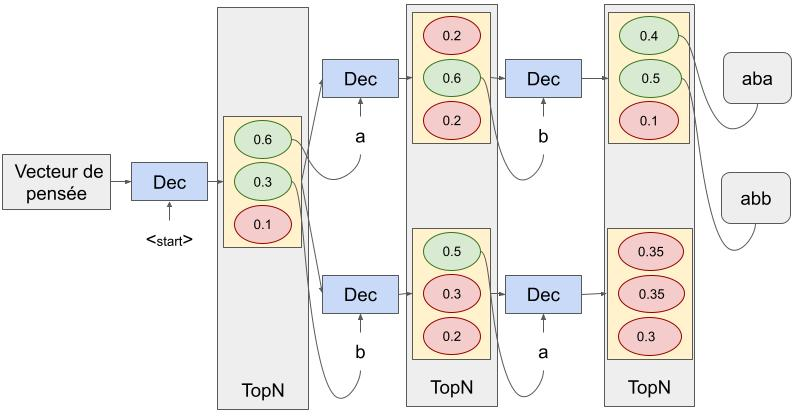
\includegraphics[scale=0.4]{2_production_mots_cles/Beam Search.jpg}
    \caption{Représentation schématique du processus de décodage grâce à l'algorithme de recherche en faisceau.}
    \label{fig:beam_search}
\end{figure}
\todo{refaire en tikz}

\`A l'inverse des algorithmes déterministes que nous avons décrits, notons l'existence des algorithmes d'échantillonnage. Ces algorithmes stochastiques choisissent les mots au hasard en fonction de leur probabilité. Les mots-clés générés par ces algorithmes ne sont donc pas reproductibles, ce qui dans le cadre de la production de mot-clés n'est pas souhaitable. Nous ne considérons donc pas cette technique.

\subsection{Paradigme encodeur-décodeur}\label{sub:paradigme_encodeur_decodeur}

Nous avons présenté dans les sections~\ref{sub:encoding} et \ref{sub:decoding} des moyens d'encoder des documents ainsi que des moyens de générer des séquences.
De nombreuses applications du traitement automatique de la langue nécessitent à la fois l'encodage d'une séquence et son décodage.
Par exemple dans le cadre de la traduction automatique, étant donnée une phrase en langue source, il faut la traduire dans une langue cible, c'est-à-dire qu'il faut encoder la phrase dans la langue source puis générer une phrase correspondante dans la langue cible.
Dans le cadre de la production de mots-clés, il faut générer un mot-clé en fonction d'un document.
Ainsi, le paradigme encodeur-décodeur introduit par \citet{sutskever_sequence_2014}, qui concatène un encodeur et un décodeur, permet de prendre en entrée une séquence de mots de longueur variable et de générer en sortie une autre séquence de mots de longueur variable.
Ce paradigme pallie la limite des réseaux de neurones présentés dans la section~\ref{sub:neural_network} (perceptrons mono ou multicouches) dont l'entrée et la sortie sont de taille fixe.

%Une fois une séquence encodée il est possible de la décoder, c'est-à-dire de produire un mot en fonction d'une représentation $h^t$.
%Générer un mot à partir d'une représentation $h_t$ consiste à passer la représentation dans un perceptron qui calcule une distribution de probabilité sur un vocabulaire, le mot à générer est choisis en fonction de sa probabilité.
    
%\begin{align}
    %\text{log}\: p(y|x) = \sum^m_{j=1} \text{log}\: p(y_j|y_{<j}, x)
%\end{align}

% FROM RECITAL SOTA

\colorlet{enccolor}{green!5}
\colorlet{inputcolor}{black!90!green}
\colorlet{deccolor}{blue!5}
\colorlet{outputcolor}{black!70!blue}
\colorlet{veccolor}{orange!15}
\colorlet{startendcolor}{black!60}
\colorlet{greybox}{black!3}

\begin{figure}[!htb]
\centering

\resizebox{\textwidth}{!}{%
\begin{tikzpicture}

\tikzstyle{cell}=[text centered, rectangle, draw, line width=.5pt, minimum height=1cm, minimum width=1.4cm, rounded corners=2pt]
\tikzstyle{word}=[font=\small\bfseries, text centered, minimum size=.5cm, minimum height=.3cm, text height=1.5ex, text depth=.25ex]
\tikzstyle{vector}=[text centered, rectangle, draw, line width=.5pt, minimum height=.5cm, minimum width=1cm, rounded corners=2pt]
\tikzstyle{arrow}=[shorten >= 2pt, shorten <= 2pt, draw=black!80]

\node[cell, fill=enccolor] (E1) at (0,0){};
\node[cell, fill=enccolor] (E2) at (2,0){};
\node[cell, fill=enccolor] (E3) at (4,0){};
\node[cell, fill=enccolor] (E4) at (6,0){};
\node[text centered] (E5) at (7.5,0){...};
\node[cell, fill=enccolor] (E6) at (9,0){};

\node[word, color=inputcolor, inner color=yellow!50, outer color=white] (I1) at (0,-1.2){Espace};
\node[word, color=inputcolor, inner color=yellow!50, outer color=white] (I2) at (2,-1.2){:};
\node[word, color=inputcolor, inner color=yellow!50, outer color=white] (I3) at (4,-1.2){la};
\node[word, color=inputcolor, inner color=yellow!50, outer color=white] (I4) at (6,-1.2){station};
%\node[word, color=inputcolor, inner color=yellow!50, outer color=white] (I5) at (8,-1.2){...};
\node[word, color=startendcolor] (I6) at (9,-1.2){<fin>};

%\node[cell, fill=veccolor, word, rotate=90] (V) at (11,0){vecteur de pensée};

\node[cell, fill=deccolor] (D1) at (11,0){};
\node[cell, fill=deccolor] (D2) at (13,0){};
\node[cell, fill=deccolor] (D3) at (15,0){};
%\node[cell, fill=deccolor] (D4) at (20,0){};

\node[word, color=startendcolor] (I7) at (11,-1.2){<début>};
\node[word, color=outputcolor, inner color=yellow!50, outer color=white] (O1) at (11,1.2){station};
\node[word, color=outputcolor, inner color=yellow!50, outer color=white] (O2) at (13,1.2){spatiale};
\node[word, color=startendcolor] (O3) at (15,1.2){<fin>};

\draw[->,>=latex,arrow] (E1) -- (E2) node[above,midway] {$h^e_0$};
\draw[->,>=latex,arrow] (E2) -- (E3) node[above,midway] {$h^e_1$};
\draw[->,>=latex,arrow] (E3) -- (E4) node[above,midway] {$h^e_2$};
\draw[->,>=latex,arrow] (E4) -- (E5) node[above,midway] {$h^e_3$};
%\draw[->,>=latex,arrow] (E5) -- (E6) node[above,midway] {$h^e_{n-1}$};
\draw[->,>=latex,arrow] (E5) -- (E6) node[above,midway] {$h^e_{n-1}$};

\draw[->,>=latex,arrow,shorten <= -2pt] (I1) to (E1);
\draw[->,>=latex,arrow,shorten <= -2pt] (I2) to (E2);
\draw[->,>=latex,arrow,shorten <= -2pt] (I3) to (E3);
\draw[->,>=latex,arrow,shorten <= -2pt] (I4) to (E4);
%\draw[->,>=latex,arrow,shorten <= -2pt] (I5) to (E5);
\draw[->,>=latex,arrow,shorten <= -2pt] (I6) to (E6);
\draw[->,>=latex,arrow,shorten <= -2pt] (I7) to (D1);


\draw[->,>=latex, arrow] (E6) -- (D1) node[above,midway] {$h^e_n$};

\draw[->,>=latex,arrow] (D1) -- (D2) node[above,midway] {$h^d_0$};
\draw[->,>=latex,arrow] (D2) -- (D3) node[above,midway] {$h^d_1$};
%\draw[->,>=latex,arrow] (D3) to (D4);

\draw[->,>=latex,arrow,shorten >= -2pt] (D1) to (O1);
\draw[->,>=latex,arrow,shorten >= -2pt] (D2) to (O2);
\draw[->,>=latex,arrow,shorten >= -2pt] (D3) to (O3);
%\draw[->,>=latex,arrow,shorten >= -2pt] (D4) to (O4);

%\node at (5,2) {\large{\textsc{Encodeur}}};
%\node at (17,2) {\large{\textsc{Décodeur}}};

\draw[arrow, rounded corners=3pt] (O1) -| (12, 0);
\draw[->,>=latex, arrow, rounded corners=3pt] (12, 0) -- (12, -1) -| (D2.south);

\draw[arrow, rounded corners=3pt] (O2) -| (14, 0);
\draw[->,>=latex, arrow, rounded corners=3pt] (14, 0) -- (14, -1) -| (D3.south);

%\draw[arrow, rounded corners=3pt] (O3) -| (19, 0);
%\draw[->,>=latex, arrow, rounded corners=3pt] (19, 0) -- (19, -1) -| (D4.south);

\draw[decoration={brace},decorate] (-0.7,1.7) -- node[below=-1.9em] {\large{\textsc{Encodeur}}} (9.7,1.7);
\draw[decoration={brace},decorate] (10.3,1.7) -- node[below=-1.9em] {\large{\textsc{Décodeur}}} (15.7,1.7);


\end{tikzpicture}
}

\caption{Exemple de modèle \textit{encodeur-décodeur} récurrent appliqué à l'extraction automatique de mots-clés.}
\label{fig:seq2seq}
\end{figure}


Le processus d'encodage et de décodage est décrit par l'équation~\ref{eq:enc-dec} et la figure~\ref{fig:seq2seq}.
Dans un premier temps la séquence d'entrée $X$ de taille $n$ est encodée dans le vecteur de pensée $h^e_n$.
Ce vecteur $h^e_n$ est utilisé pour initialiser le premier état caché du décodeur $h^d_0$.
Le décodeur génère ensuite les mots $\hat{y}_t$ qui composent la séquence de sortie $\hat{Y}$ à partir de cet état caché.

\begin{equation}\label{eq:enc-dec}
  \begin{split}
    p(\hat{y}_t | y_{1,...,t-1},h_0) & = \textsc{Softmax}(\sigma(b_v + W_v * h^d_t)) \\
    h^d_t & = \textsc{Rnn}^d(\hat{y}_{t-1}, h^d_{t-1}) \\
    \hat{y}_0 & = \textsc{Debut} \\
    h^d_0 & = h^e_n \\
    h^e_n & = \textsc{Rnn}^e(X) \\
  \end{split}
\end{equation}

Nous présentons ci-après deux améliorations de ce paradigme.
%
D'abord, le mécanisme d'attention qui permet de porter attention à une partie spécifique de l'entrée lors du décodage. Par exemple, la description d'une image nécessite d'identifier les différents objets qui la composent.
%
Ensuite, le mécanisme de copie qui pallie l'incomplétude du vocabulaire de sortie. Ce mécanisme permet au décodeur de copier un mot du document d'entrée au lieu de le générer à partir du vocabulaire de sortie. Le mécanisme de copie est particulièrement utile pour les entités nommées par exemple. Ces entités sont peu fréquentes et ne font généralement pas partie du vocabulaire de sortie.

% Convolution
%Les réseaux de neurones à convolution sont surtout utilisés pour le traitement d'images. Dans le cas du texte, des 
    
% Graphes
%Les réseaux à convolution de graphes (GCN) permettent d'obtenir pour chaque noeud d'un graphe un embedding en fonction de ses voisins. Le nombre de convolutions représente le nombre de bonds qui sont fait entre les noeuds.
    
% Transformer
%Les transformer ont été introduit par \cite{vaswani_attention_2017} et utilisent un mécanisme de self-attention pour chaque mot d'une séquence, de sorte à obtenir pour chaque mot un vecteur qui représente sa relation avec chaque autre mot. Ce mécanisme ne prend pas en compte la séquentialité, en effet chaque calcul est parallélisable. Et ce modèle qui requiert une force de calcul colossale a montré de très bons résultats sur de nombreuse tâches.

\subsubsection{Mécanisme d'attention}
\label{sub:attention_mecanism}

Le mécanisme d'attention~\cite{bahdanau_neural_2014,luong_effective_2015} a été introduit pour améliorer le traitement de longues séquences en permettant au modèle de se focaliser sur certaines parties du document lors du décodage.
%
En effet, un mot-clé concerne seulement certains aspects d'un document. Ce mécanisme permet donc au modèle de porter attention aux parties du document liées à ces aspects.
%
De plus, cette attention au document peut être visualisée grâce aux \emph{poids d'attention} calculés à chaque étape de décodage.
%Par exemple, dans le cadre de la traduction automatique, il permet de visualiser l'alignement entre la phrase en langue source et la phrase en langue cible.
%Par exemple, dans le cadre de la traduction automatique, ce mécanisme permet de visualiser l'importance de chaque mot du document source pour générer la traduction.
La figure~\ref{fig:attention_alignment} illustre cette attention dans le cadre de la traduction automatique pour traduire en français la phrase \say{The agreement on the European Economic Area was signed in August 1992.}
%Il existe généralement un alignement monotone entre les phrases en français et les phrases en anglais.
%Mais ce n'est pas toujours le cas comme le montre le syntagne nominal \say{European Economic Area} dont les mots de la traduction sont dans un ordre inverse \say{zone économique européenne}.
%Le modèle a pu, grâce au mécanisme d'attention, proposer la bonne traduction \say{zone économique européenne} dont l'ordre des mots est inverse à sa traduction.
% Même si le français et l'anglais peuvent généralemnt être traduit mot à mot de manière monotone, le mécanisme d'attention nous permet de visualiser l'alignement non monotone entre zone économique européenne et European Economic Area, en effet l'ordre des noms et adjectifs en français et en anglais est différent.
%Ainsi nous pouvons observer que pour traduire \say{was} en \say{a été}, le modèle à porté attention à \say{was signed} pour comprendre que \say{was} fait parti de la construction du prétérit.
%Pour illustrer ce mécanisme dans le cadre de la traduction automatique nous prenons l'exemple suivant: pour traduire la séquence \say{the European Economic Area} en français (\say{\foreign{la zone économique européenne}}) le modèle portera attention à chaque mot du texte source. Ainsi, pour générer \say{la} et \say{zone} il devra porter attention à \say{\foreign{the}} et \say{\foreign{Area}}. \todo{A revoir.}

\begin{figure}
    \centering
    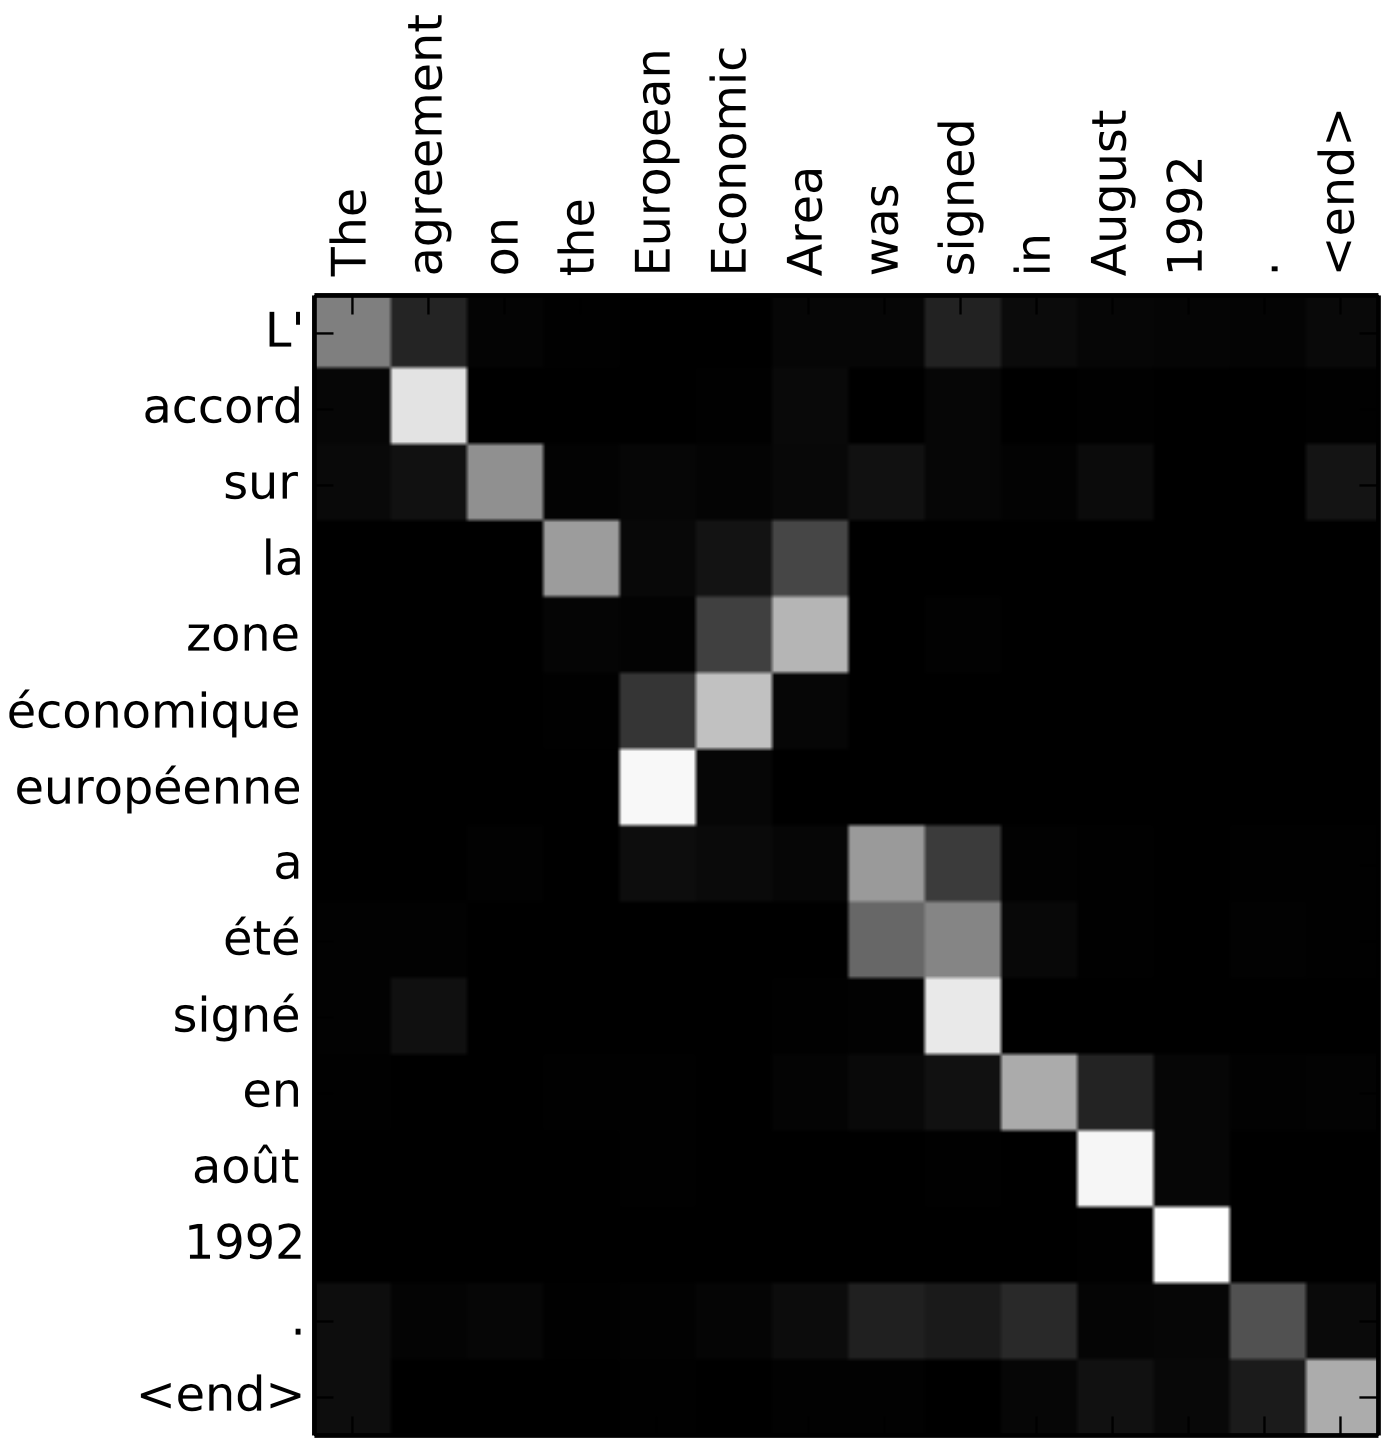
\includegraphics[scale=0.3]{2_production_mots_cles/attention_alignment.png}
    \caption{Exemple de visualisation des poids d'alignement du mécanisme d'attention entre une phrase en anglais et sa traduction en français. Chaque ligne montre la distribution des poids $\alpha_{t}$ ayant servis à générer le mot correspondant en français. Une case blanche indique un poids de 1, une case noire indique un poids de 0. Image extraite de \citet{bahdanau_neural_2014}.}
    \label{fig:attention_alignment}
\end{figure}

%Il faudra aussi porter attention à la syntaxe des deux langues
%Les poids d'attention peuvent être utilisés pour visualiser l'alignement entre les mots de la séquence d'entrée et ceux de la séquence de sortie.
%La figure~\ref{fig:attention_alignment} montre les poids d'alignement dans le cadre de la traduction automatique entre une phrase en anglais et sa traduction en français.

Le décodeur utilise l'état caché courant $h^d_t$ pour générer un mot, le mécanisme d'attention lui permet d'utiliser aussi tous les états cachés de l'encodeur $h^e$ pour mettre à jour l'état caché du décodeur $h^d_t$. Ce mécanisme est décrit dans l'équation~\ref{eq:attention}.
Dans le mécanisme d'attention, les états cachés $h^e$ sont pondérés en fonction de leur importance pour générer le mot $\hat{y}_t$.
Cette importance est établie grâce à une fonction d'alignement $a$ qui calcule une similarité entre l'état caché courant $h^d_t$ et ceux de l'encodeur $h^e$.
Les états cachés $h^e$ sont ainsi moyennés dans le vecteur de contexte $c_t$ utilisé pour mettre à jour l'état caché courant du décodeur $h^d_t$.

Dans l'équation \ref{eq:attention}: $[u;v]$ représente l'opération de concaténation des vecteurs $u$ et $v$; $a$ est une fonction d'alignement qui calcule la similarité entre un état caché de l'encodeur $h^e_t$ et du décodeur $h^d_t$; $\alpha$ représente les poids d'alignement entre les états cachés de l'encodeur $h^e$ et du décodeur $h^d$;  et $\textsc{Softmax}$ est une fonction qui normalise les valeurs d'un vecteur pour qu'il somme à 1.


\iffalse
    \begin{figure}
        \centering
        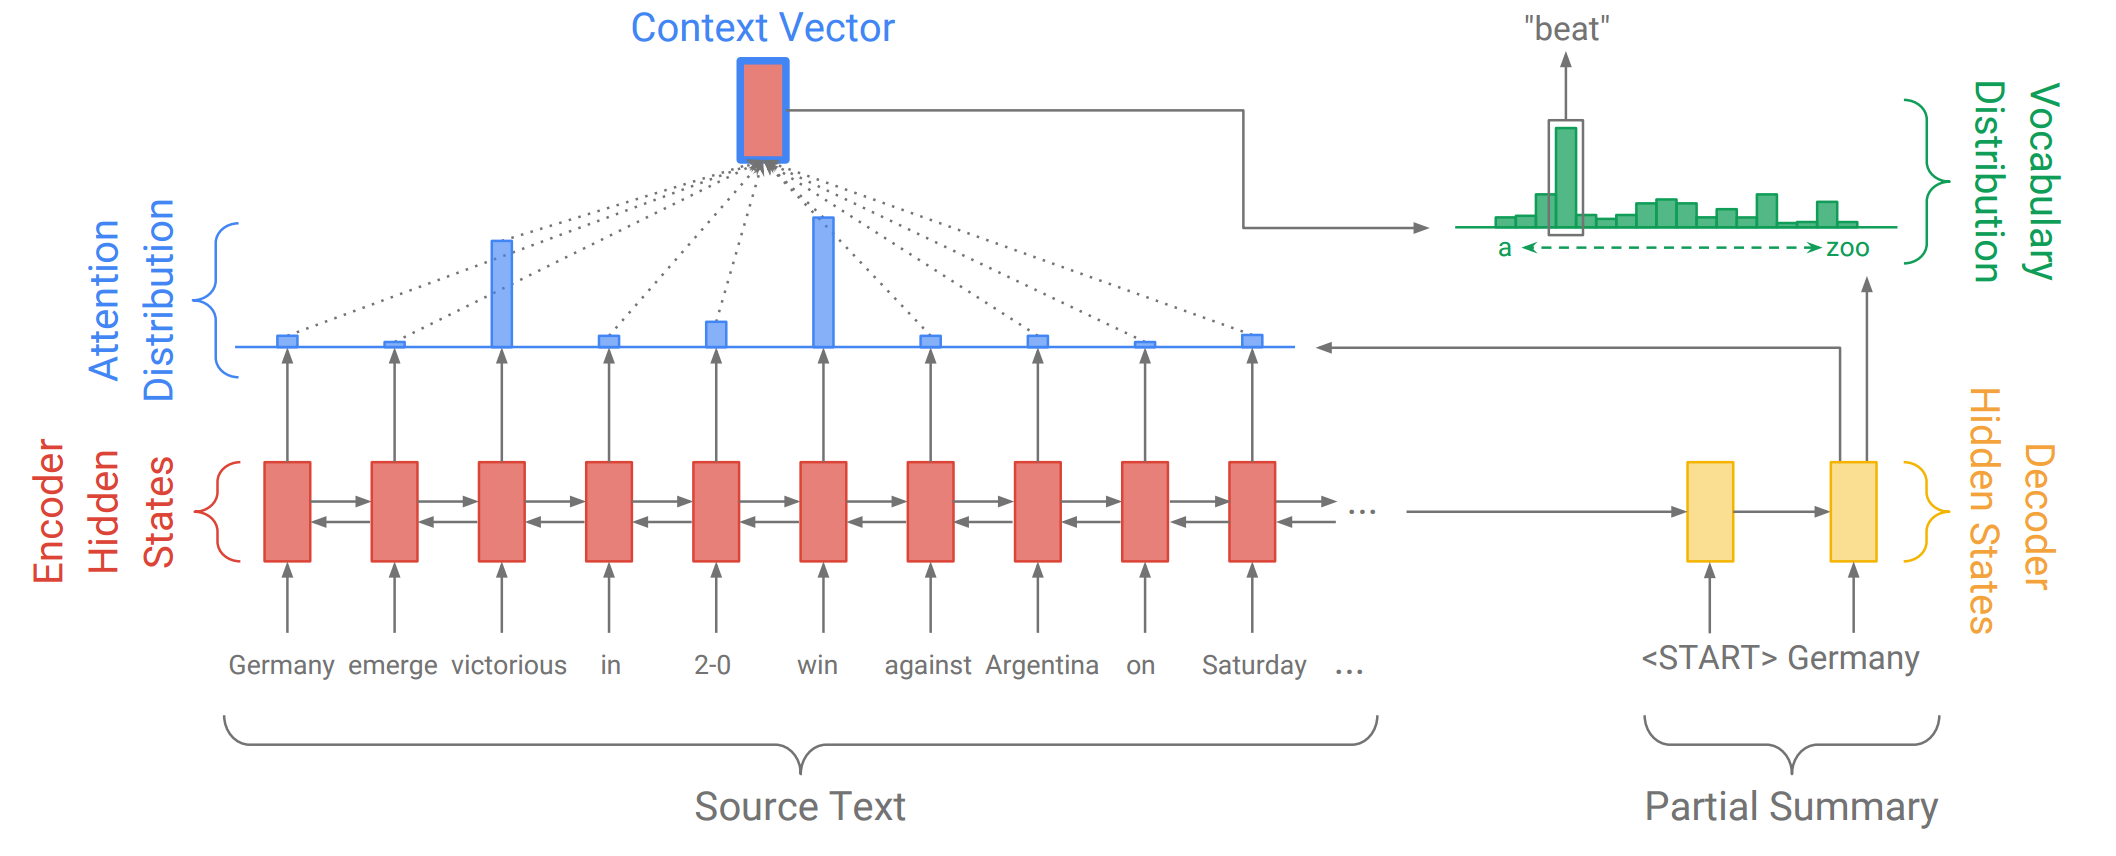
\includegraphics[width=\linewidth]{figures/see_seq2seq-attn.png}
        \caption{Schéma du mécanisme de copie présenté par \cite{see_get_2017}.}
        \label{fig:see_attention}
    \end{figure}
\fi

\begin{equation}\label{eq:attention}
  \begin{split}
    %\hat{Y}_t & = \sigma(b_v + W_v * h^d_t) \\
    p(y_t|y_{<t},x) & = \textsc{Softmax}(\sigma(W_v h^d_t)) \\[.3em]
    h^d_t & = \textsc{Rnn}(y_{t-1}, [h^d_{t-1};c_t]  \\[.3em]
    c_t & = \sum^{|h^e|}_{i=0} \alpha_{i,t} h^e_i \\
    \alpha_{t} & = \textsc{Softmax}(a(h^d_t, h^e)) \\
    %\textsc{Softmax}(x) & = \left[ \frac{x_i}{\sum^{|x|}_{i=0} x_i} , i \in |x| \right]
  \end{split}
\end{equation}

%Le concept d'attention a été présenté de deux manières différentes par \cite{bahdanau_neural_2014} et \cite{luong_effective_2015}.
%
%L'idée de l'attention présentée par~\cite{luong_effective_2015} est \emph{d'utiliser le vecteur de contexte pour prédire $y_t$}.
%
%\cite{bahdanau_neural_2014} présente un autre mécanisme d'attention dont l'idée est de calculer l'état caché du décodeur à l'aide d'un vecteur de contexte. Par rapport à un décodeur classique, seul le calcul de $h^d_t$ change.

\iffalse
    L'idée de l'attention présentée par~\cite{luong_effective_2015} est \emph{d'utiliser le vecteur de contexte pour prédire $y_t$}.
    
    Pour cela, un nouveau $\hat{h}^d_t$ est calculé en fonction d'un vecteur de contexte $c_t$ et de $h^d_t$ (calculé en fonction de $y_{t-1}$ et $h^d_{t-1}$). $c_t$ est la moyenne des $h^e$ pondérés par les scores d'alignement $\alpha$.
    
    Dans leur article, deux manières de calculer l'attention sont présentées: une attention globale et une attention locale.
    %
    Pour l'attention globale, le vecteur de contexte est la moyenne pondérée de toutes les représentations de l'encodeur.
    %
    Pour l'attention locale, le vecteur de contexte est la moyenne pondérée des représentations $h^e$ dans une fenêtre de taille $D$ autour de $h^e_{p_t}$.
    %
    $p_t$ est une valeur entre 0 et $|h^e|$ qui définit le centre de la fenêtre, et peut être calculé de différentes manières.\footnote{Pour plus de détails voir la section 3.2 de \cite{luong_effective_2015}}
    %$p_t$ étant $t$ (dans la traduction automatique on considère que le mot cible $y_t$ est aligné avec le mot source $x_{p_t}$), ou alors un réel entre 0 et $|h^e|$ calculé à l'aide 
    
    \begin{align}
        %y_t & = \sigma(W_v h^d_t) \\
        p(y_t | y_{<t}, x) & = \textsc{Softmax}(W_v \hat{h}^d_t) \\
        \hat{h}^d_t & = \sigma(W_c [c_t;h^d_t]) \\
        c_t & = \sum^{|h^e|}_{i=0} \alpha_{i,t} * h^e_i \\
        \alpha_{i,t} & = \textsc{Softmax}(a(h^e_i, h^d_t)) \\
        h^d_t & = \textsc{Rnn}(y_{t-1}, h^d_{t-1})
    \end{align}
    
    \cite{bahdanau_neural_2014} présente un autre mécanisme d'attention dont l'idée est de calculer l'état caché du décodeur à l'aide d'un vecteur de contexte. Par rapport à un décodeur classique, seul le calcul de $h^d_t$ change. Le calcul du vecteur de contexte est similaire à celui de ~\cite{luong_effective_2015}.
    
    \begin{align}
        p(y_t|y_{<t},x) & = \textsc{Softmax}(W_v h^d_t) \\
        h^d_t & = \textsc{Rnn}(y_{t-1}, [h^d_{t-1};c_t]  \\
        c_t & = \sum^{|h^e|}_{i=0} \alpha_{i,t} * h^e_i \\
        \alpha_{i,t} & = \textsc{Softmax}(a(h^e_i, h^d_t))
    \end{align}
    
    Il existe différentes fonctions d'alignement:
    
    bahdanau $a(h^e_i, h^d_t) = v_a \text{tanh}(W_a h^d_t + U_a h^e_i)$
    
    dot $a(h^e_i, h^d_t) = h^e_i h^d_t$
    
    general $a(h^e_i, h^d_t) = h^e_i W_a h^d_t$
    
    concat $a(h^e_i, h^d_t) = W_a [h^e_i;h^d_t]$
\fi

\subsubsection{Mécanisme de copie}
\label{sub:copy_mecanism}

Le mécanisme de copie~\cite{see_get_2017,gu_incorporating_2016} provient des tâches de traduction automatique et de résumé automatique. Il a pour but de produire des mots peu fréquents ou hors du vocabulaire de sortie.
En effet, les modèles neuronaux qui génèrent du texte choisissent les mots dans un vocabulaire de sortie comportant généralement \num{50 000} mots.
Dans les tâches sus-citées, les mots peu fréquents qui ne font pas partie du vocabulaire de sortie, comme les entités nommées ou les transfuges, doivent pourtant apparaître dans la séquence de sortie.
%Le mécanisme de copie ~\cite{see_get_2017,gu_incorporating_2016} pallie ce problème en permettant au décodeur de générer un mot du vocabulaire de sortie ou bien de copier un mot du document.
Deux mécanismes de copie ont été proposés par \citet{see_get_2017} et \citet{gu_incorporating_2016}; les deux étant similaires, nous présentons ici le premier car plus simple. Il est décrit dans l'équation~\ref{eq:copy_mecanism}.

% exemple
%Le mécanisme d'attention a été utilisé comme post-traitement pour remplacer les mots inconnus de la sortie par les mots de l'entrée alignés par le mécanisme d'attention. Ceci permettant de traiter les entités nommées peu fréquentes ou les transfuges.
%
%Le mécanisme de copie vient automatiser ce processus en permettant au modèle de générer un mot du vocabulaire ou de copier un mot du document.

%, tous deux inspirés des réseaux de pointeurs~\cite{vinyals_pointer_2015} qui génèrent une séquence de pointeurs vers la séquence d'entrée.
Ce mécanisme utilise le vocabulaire de la séquence d'entrée $\mathcal{X}$ (particulier à chaque document) en plus du vocabulaire de sortie $\mathcal{V}$.
Pour produire un mot, une distribution de probabilité sur le vocabulaire  $P_{vocab}(y_{t})$ est calculée comme précédemment par le décodeur (cf. section~\ref{sub:decoding}) et les poids du mécanisme d'attention $\alpha$ (cf. section~\ref{sub:attention_mecanism}) sont utilisés pour estimer la probabilité de copie de chaque mot du document.
Les poids d'attention $\alpha$ des mots qui apparaissent plusieurs fois dans l'entrée $x$ sont sommés $\sum_{j,x_j=y_{t,i}} \alpha^t_j$.
Ainsi, un mot peut être généré à partir du vocabulaire de sortie $\mathcal{V}$ ou copié à partir du vocabulaire du document $\mathcal{X}$.
Les probabilités de copie et de génération d'un même mot, qui appartient au document et au vocabulaire, sont sommées.
Dans l'équation~\ref{eq:copy_mecanism}: $h^d_t$, $c_t$ et $\alpha^t_j$ proviennent du mécanisme d'attention (cf. équation~\ref{eq:attention}); $p_{gen}$ est un curseur permettant au modèle de privilégier la copie ou la génération et $P_{vocab}(y_t)$ est une distribution de probabilité sur le vocabulaire de sortie $\mathcal{V}$.

%Les probabilités de génération et de copie sont combinés pour donner une distribution de probabilités sur $\mathcal{X} \cup \mathcal{V}$.

\begin{equation}\label{eq:copy_mecanism}
  \begin{split}
    p(y_{t,i}|y_{<t},x) & = p_{gen} P_{vocab}(y_{t,i}) + (1 - p_{gen}) \sum_{j,x_j=y_{t,i}} \alpha^t_j \\
    p_{gen} & = \sigma(W_h h^d_t + W_c c_t + W_y y_{t-1}) \\
    P_{vocab}(y_{t}) & = \textsc{Softmax}(\sigma(W_v h^d_t))
  \end{split}
\end{equation}

%ou les poids d'un mécanisme d'attention supplémentaire, utilisé seulement pour calculer le score de copie, pour~\cite{gu_incorporating_2016}

\iffalse
    %\cite{gu_incorporating_2016}, création d'un vocabulaire spécifique a chaque instance, composé de $\mathcal{V}$ le vocabulaire normal et $\mathcal{X}$ le vocabulaire des mots de l'entrée.
    %
    %Ça change le calcul de $y_t$ par rapport au mécanisme d'attention.
    %
    %On défini les vecteurs $\psi_g \in \mathds{R}^|\mathcal{V}|$ et $\psi_c \in \mathds{R}^|\mathcal{X}|$ qui contiennent respectivement les score de copie et de génération.
    
    % attentive read = les poids de l'attention
    % selective read = les poids de l'"attention" du mécanisme de copie
    
    \begin{align}
        y_t & = \textsc{Softmax}(e^{P_{gen}} +e^{P_{copy}}) \\
        P_{gen} & = W_v h^d_t \\
        P_{copy} & = \left[ \sum^{|h^e|}_{j=0, x_j=x_i} \sigma(h^e_j W_c) h^d_t | x_i \in \mathcal{X} \right] \\
        h^d_t & = RNN([y_{t-1};cc_t)],h^d_{t-1}) \\
        cc_t & = \sum^{|h^e|}_{i=1} aa_{t,i} h^e_t \\
        aa_{t,i} & = \textsc{Softmax}()
    \end{align}
    
    %\cite{see_get_2017} reprend le mécanisme d'attention de \cite{luong_effective_2015} et modifie le calcul de $y_t$ en ajoutant une probabilité de copie et un curseur privilégiant la copie ou la génération.
    
    \begin{align}
        p(y_{t,i}) = p_{gen} P_{vocab}(y_{t,i}) + (1 - p_{gen}) \sum_{j,x_j=y_{t,i}} \alpha^t_j \\
        p_{gen} = \sigma(W_c c_t + W_h h^d_t + W_y y_{t-1})
    \end{align}
\fi

% Multitache
% Conditional Random Field
% Reinforcement Learning : adaptative reward


\section{Méthodes de bout-en-bout}
\label{methodes-de-bout-en-bout}

\todo{Ajouter des schéma pour mieux comprendre les méthodes.}

Dans cette section nous présentons un état de l'art des méthodes de bout-en-bout.
Ces méthodes, contrairement aux méthodes en chaîne de traitement (cf. section~\ref{sec:methode-en-chaine-de-traitement}), prennent en entrée un document et laissent le soin au modèle d'en extraire les caractéristiques pour retourner un ensemble de mots-clés sans étapes intermédiaires ni définition manuelle de ces caractéristiques.
Parmi les méthodes proposées dans la littérature, nous distinguons les méthodes génératives, qui peuvent produire des mots-clés présents et des mots-clés absents, des méthodes extractives, limitées aux mots-clés présents.

Jusqu'à présent, toutes les méthodes de bout-en-bout qui ont été proposées sont supervisées et reposent sur des réseaux de neurones (cf. section~\ref{sub:neural_network}) qui nécessitent de grandes quantités de données annotées pour être entraînées.
%
Le développement de ces méthodes démarre avec l'introduction du jeu de données KP20k et de la méthode générative CopyRNN par \citet{meng_deep_2017}.
Le jeu de données KP20k, qui comporte $\simeq$\num{550000} documents, comble un manque.
En effet, seuls de petits jeux de données (de l'ordre du millier de documents) étaient jusqu'alors disponibles.
Ce travail a ainsi lancé une nouvelle direction de recherche sur les méthodes génératives de production de mot-clés.

\begin{figure}
    \centering
    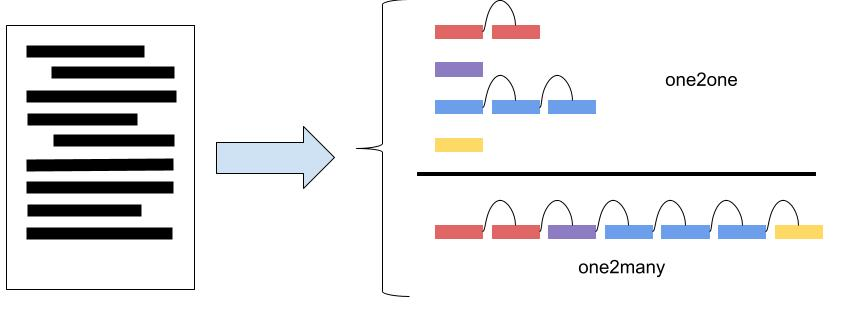
\includegraphics[scale=0.4]{2_production_mots_cles/Decoding strategies.jpg}
    \caption{Représentation schématique des stratégies de décodage \emph{one2one} et \emph{one2many}.}
    \label{fig:decoding_strategies}
\end{figure}
\todo{Refaire en tikz}

Dans cet état de l'art, nous présentons tout d'abord les méthodes automatiques de génération de mots-clés de bout-en-bout, qui sont au c\oe{}ur de ce travail de thèse.
Nous présentons ces méthodes de génération en deux parties: premièrement, les méthodes qui générent les mots-clés un à un (\emph{one2one}), et deuxièmement, celles qui génèrent des séquences de mots-clés (\emph{one2many}). Ces deux types de génération sont schématisés dans la figure~\ref{fig:decoding_strategies}.
Nous présentons ensuite les méthodes extractives de bout-en-bout, c'est-à-dire celles qui se limitent aux seuls mots-clés présents.

\subsection{Génération de mots-clés}
\label{sub:generation_de_mots_cles}

Les méthodes génératives, introduites par \citet{meng_deep_2017}, ont pour objectif de pallier deux faiblesses qui concernent la majorité des méthodes extractives présentées précédemment: l'impossibilité de produire des mots-clés absents ainsi que la faible prise en compte de la sémantique.
Le paradigme encodeur-décodeur sur lequel les méthodes génératives sont fondées permet d'encoder la sémantique du document.
Ainsi, les mots-clés produits sont le fruit d'une \say{compréhension} du document, contrairement aux méthodes en chaîne de traitement qui s'intéressent à l'\say{importance} des mots dans le document indépendamment de leur sens.
%
Ces méthodes génératives rendent possible la production de mots-clés absents grâce à la manière dont le décodeur génère la séquence de sortie.
Ce processus s'effectue en choisissant, à chaque étape de décodage, un mot à partir d'un vocabulaire de sortie qui est plus grand et différent du vocabulaire du document.
Ces méthodes génératives apprennent à générer des mots-clés un par un (génération \emph{one2one}, voir figure~\ref{fig:decoding_strategies}), c'est-à-dire que chaque document $X$ et son ensemble de mot-clés $Y$ de taille $N$ forment un couple $(X, \{Y_0, ..., Y_N\})$, décomposé en autant d'exemples d'entraînement que de mots-clés, $(X, Y_0), ... , (X, Y_N)$.

%\paragraph{Définitions}
%\todo{Il faudrait définir avant les principaux modèles: one2one, séquence avant de les définir formellement; Fait ausi des dessins}
%$x$ et $y$ représentent des mots, $p$ des mots-clés. Étant donné un ensemble de données $D = {(x^i,p^i), i \in 1...N}$ de taille $N$, un exemple est composé d'un document $x^i$ et d'un ensemble de mots-clés $p^i = {p^i_j, j \in 1...M^i}$ de taille $M^i$. Les documents et les mots-clés sont composés de mots $[x^i_k, k \in 1...N^i]$ et $[y^i_j]$ est composé d'un document composé d'une séquence de mots $x^i = (x^i_1, ..., x^i_{N^i})$ de longueur $N^i$ et d'un ensemble de mots-clés $p^i$ de taille $M^i$ avec $p^i = (p^i_1, ..., p^i_{M^i})$, où chaque mot-clé est une séquence de mots de taille $M^{i,j}$ avec $p^{i,j} = (y^{i,j}_1, ..., y^{i,j}_{M^{i,j}})$. Dans le cadre des modèles one2one, un couple document -- mots-clés est découpé en $M^i$ différents couples $(x^i, p^{i,1}), ..., (x^i, p^{i, M^i})$. 
%Pour les modèles en séquences, les mots-clés sont concaténés de sorte à former une unique séquence $(x^i, y^{i,1}_1 \lozenge ... \lozenge y^{i,1}_{M^{i,j}} \lozenge \text{SEP} \lozenge y^{i,2}_1 \lozenge ... \lozenge y^{i,M^i}_{M^{i,j}})$.

La méthode pionnière de génération automatique de mots-clés appliquée aux documents scientifiques est CopyRNN~\cite{meng_deep_2017}.
%
L'architecture neuronale de cette méthode s'inspire du processus d'annotation humain qui consiste à lire le document pour le comprendre dans son entièreté puis à le résumer grâce à des mots-clés.
%Aussi, les humains peuvent facilement s'abstraire du texte et faire appel à leurs connaissances pour produire des mots-clés qui n'apparaissent pas dans le texte.
Pour reproduire ce processus, CopyRNN utilise le paradigme encodeur-décodeur, que nous avons présenté dans la section~\ref{sub:paradigme_encodeur_decodeur}, pour encoder un document et le décoder ensuite en un mot-clé. % Ainsi un réseau de neurones récurrent encode le document dans un vecteur de pensée, puis un autre décode, génère, ce vecteur de pensée en un mot-clé.
Pour améliorer les performances des modèles encodeur-décodeur, il est commun d'utiliser un mécanisme d'attention (voir section~\ref{sub:attention_mecanism}).
Ce mécanisme permet au modèle de porter attention à certaines parties du document lors de la génération d'un mot.
%
Un mécanisme de copie est aussi ajouté au modèle pour lui permettre de générer des mots peu fréquents (voir section~\ref{sub:copy_mecanism}).
Ce mécanisme de copie modifie le décodage en permettant de générer un mot à partir du vocabulaire de sortie ou bien à partir du document.\\
%
Cette méthode obtient des performances bien plus élevées que les précédentes méthodes extractives. Les performances de CopyRNN sont de l'ordre de 30 points de \fmesure{} pour les mots-clés présents tandis que les performances des méthodes extractives sont généralement en dessous de 20 points de \fmesure{}.
Les mots-clés absents, qui ne pouvaient jusque-là pas être produits, correspondent peu à la référence: parmi les 50 meilleurs mots-clés absents un seul apparaît dans la référence.


%La communauté scientifique présente de nouvelles méthodes basées sur CopyRNN et tente de l'améliorer.
% les méthodes essaient de résoudre les problèmes identifiés
%Les méthodes présentées augmentent toujours les performances de génération des mots-clés présents et absents.

Certaines méthodes proposées essaient d'améliorer l'encodage du document.
\citet{chen_title-guided_2019}, par exemple, constate que les mots-clés ne sont pas uniformément distribués dans les documents.
En particulier \npercent{60} des mots-clés de référence ont au moins un mot en commun avec le titre du document.
Pour prendre cela en compte, ils proposent TGNet (Title Guided Network), qui étend CopyRNN en introduisant un nouvel encodeur spécifique au titre, en plus de l'encodeur du document.
Cet encodage du titre permet de donner un poids supplémentaire à l'information qu'il contient.
Ces deux représentations (du titre et du document) sont ensuite combinées puis fournies au décodeur.
Cette méthode améliore nettement les performances de génération des mots-clés présents et absents par rapport à CopyRNN (+\npercent{5} sur KP20k).
% Ils ne regardent que la F-mesure présent/absent rien d'autre

La redondance dans les ensembles de mots-clés produits est un problème récurrent dans les méthodes de production de mots-clés.
En effet, \citet{hasan_automatic_2014} montrent que 8 à \npercent{12} des erreurs des méthodes sont liées à la redondance des mots-clés.
Ainsi, les méthodes en chaîne de traitement mettent en place des stratégies, notamment lors de la sélection du sous-ensemble de mots-clés, pour limiter cette redondance (voir section~\ref{choisir-le-sous-ensemble}).
Dans cette ligne de recherche, \citet{zhao_incorporating_2019} remarquent les méthodes de bout-en-bout ne sont pas exemptes de ce problème, ils s'intéressent ainsi au chevauchement entre les mots-clés générés et ceux de référence.
Par exemple, \npercent{23.98} des mots-clés unigrammes générés par CopyRNN font partie d'un mot-clé de référence, et \npercent{47.15} des mots-clés 4-grammes générés par CopyRNN contiennent un mot-clé de référence.
Dans l'optique de limiter ces chevauchement, ils présentent le modèle ParaNet$_T$+CoAtt qui entraîne le modèle, à générer à la fois les mots-clés et leurs étiquettes morphosyntaxiques, ainsi la syntaxe des mots-clés générés sera similaire à celle des mots-clés de référence.
Pour cela ils ajoutent au modèle CopyRNN un encodeur, pour les étiquettes morphosyntaxiques des mots du document, ainsi qu'un décodeur, pour celles du mot-clé.\footnote{Les étiquettes morphosyntaxiques du document et des mots-clés proviennent de l'outils Stanford CoreNLP.}
Les informations des deux décodeurs sont ensuite combinées et utilisées pour générer les mots-clés et leurs étiquettes morphosyntaxiques.
%Grâce à cette méthode, les mots-clés générés chevauchent moins les mots-clés de référence; par exemple le pourcentage de mot-clés 4-grammes contenant un mot-clé de référence a baissé de \npercent{10}.

\begin{figure}
    \centering
    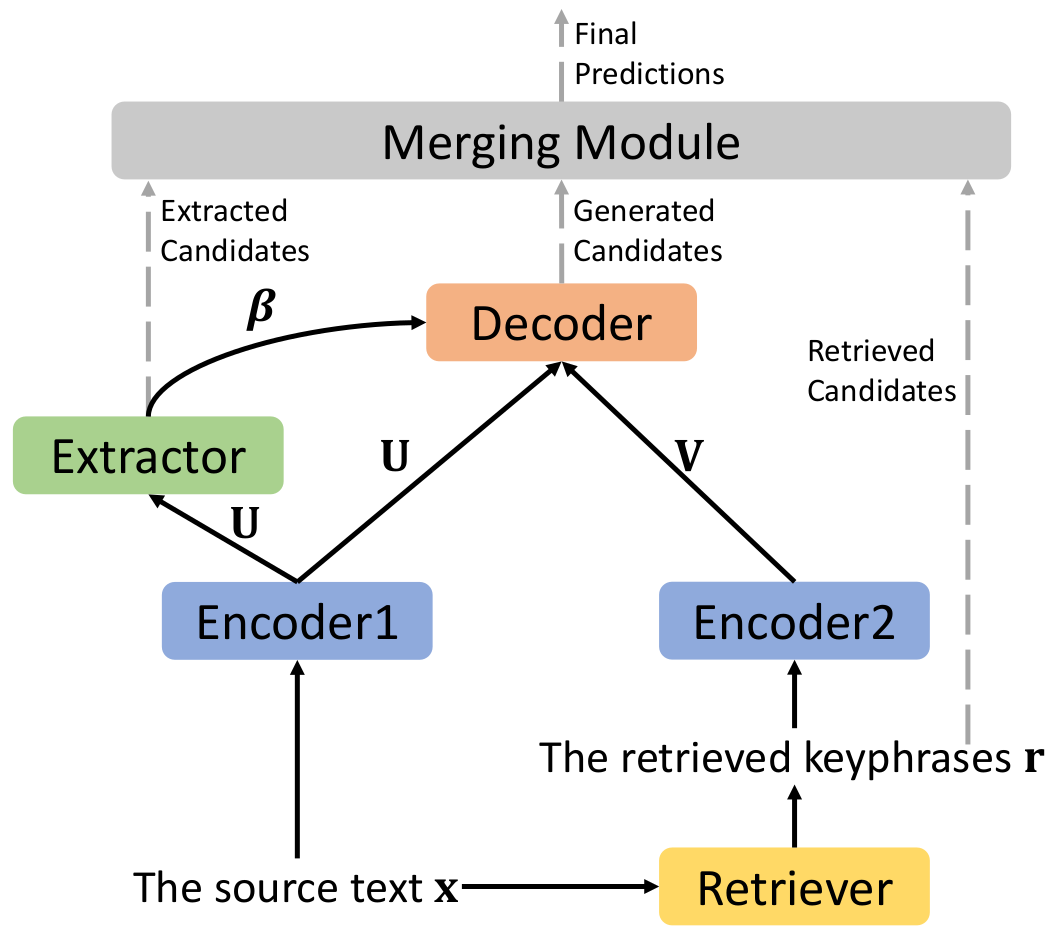
\includegraphics[scale=0.2]{2_production_mots_cles/kg_ke_kr_m.png}
    \caption{Représentation schématique de l'architecture de la méthode KG-KE-KR-M. Image extraite de~\citet{chen_integrated_2019}.}
    \label{fig:schema_kgkekrm}
\end{figure}

%Le processus manuel d'annotation en mots-clés est composé de plusieurs étapes: la lecture du document, l'extraction des mots-clés dans le document puis l'attribution de mots-clés absents du document et enfin la combinaison des mots-clés provenant de ces deux processus d'annotation.
Dans l'optique de reproduire l'annotation humaine, \citet{chen_integrated_2019} propose la méthode KG-KE-KR-M qui produit un ensemble de mots-clés en combinant différentes méthodes: génération de mots-clés, extraction de mots-clés, récupération de mots-clés (voir figure~\ref{fig:schema_kgkekrm}).
%Ces différentes méthodes sont entraînées de bout-en-bout puis les mots-clés de chaque méthode sont pondérés grâce à un classifieur.
%
Dans un premier temps, cette méthode récupère les mots-clés de référence des $K$ documents d'entraînement les plus proches du document traité (grâce à la distance de Jaccard).
Ces mots-clés \emph{récupérés} sont concaténés puis encodés. Ils serviront à conditionner la génération de mots-clés.
Dans un second temps, des mots-clés sont \emph{extraits} du document en classifiant chaque mot comme mot-clé ou non mot-clé.
%Cette classification s'effectue grâce aux états cachés du document encodé.
Ensuite, des mots-clés sont \emph{générés} à partir du document ainsi que des mots-clés récupérés et des mots-clés extraits.
Enfin, les mots-clés récupérés, extraits et générés sont pondérés grâce à un classifieur.
Cette méthode à la particularité de combiner les méthodes en chaîne de traitement (sélection de candidats puis pondération) et les méthodes de bout-en-bout (apprentissage conjoint de la génération et de l'extraction).
Malgré la grande diversité dans les techniques de production de mots-clés candidats, les performances ne sont pas significativement supérieures à CopyRNN. Cette méthode produit néanmoins plus de mots-clés absents de référence que CopyRNN.

La méthode CorrRNN~\cite{chen_keyphrase_2018} considère que les mots-clés doivent couvrir l'ensemble des sujets du document et être divers, c'est-à-dire que chaque mot-clé doit concerner un sujet différent.
Cette méthode étend CopyRNN en y ajoutant un mécanisme de couverture et un mécanisme de revue.
Le mécanisme de couverture encourage le modèle à porter attention aux différentes parties du document.
Il conserve et accumule les scores d'attention des mots du document à chaque étape de décodage, et il est inclus dans le calcul du mécanisme d'attention.
Ensuite, le mécanisme de revue est essentiellement un mécanisme d'attention sur les mots générés.
Son objectif est d'identifier les sujets déjà couverts par les mots-clés générés et ainsi de générer des mots-clés qui concernent des sujets non traités.
Cette méthode est la première à prendre en compte les mots-clés déjà générés dans le processus de génération, pour cela la phase d'entraînement est modifiée.
Au lieu de rétro-propager le gradient après chaque mot-clé de référence, la phase de rétro-propagation n'est effectuée qu'une fois tous les mots-clés de référence du document traités.
%Chaque mot-clé est généré en utilisant les mécanismes de couverture et de redondance, qui prennent en compte les mots-clés déjà générés; le gradient est ensuite calculé grâce à l'erreur de chaque mot-clé; et enfin, rétro-propagé.
%Cette méthode améliore les performance de production de mots-clés présent par rapport à CopyRNN, mais l'article ne présentant pas ses résultats sur le jeu de données de référence KP20k et utilisant des métriques peu utilisés dans les autres travaux la comparaison est limitée.

\subsection{Génération de séquences de mots-clés}% (\textsc{One2Seq})}
%\subsection{Génération en séquence}
\label{sub:generation_de_sequences_de_mots_cles}

%Nous avons présenté dans la section précédente, des méthodes génératives qui apprennent à générer un mot-clé par document.
Nous présentons dans cette section des méthodes qui apprennent à générer des séquences de mots-clés (génération \emph{one2many}, voir figure~\ref{fig:decoding_strategies}). C'est-à-dire que chaque exemple d'entraînement est composé d'un document et de la concaténation des mots-clés de référence en une unique séquence dans laquelle ils sont séparés par un symbole de séparation. Par exemple, l'ensemble de mots-clés $\{$ Classe , Fichier log , Agrégat $\}$ sera transformé en \say{Classe \texttt{SEP} Fichier log \texttt{SEP} Agrégat \texttt{FIN}}.
%Le développement des méthodes utilisant la génération \emph{one2many} part du constat que la génération \emph{one2one} ne permet pas de prendre en compte les mots-clés déjà générés et que les ensembles de mots-clés sont souvent redondants~\cite{hasan_automatic_2014}.
Le développement des méthodes génératives \emph{one2many} part du constat que les ensembles de mots-clés produits sont souvent redondants~\cite{hasan_automatic_2014} et que la génération \emph{one2one} ne permet pas de pallier ce problème.
En effet, les méthodes \emph{one2many} font l'hypothèse qu'avec la génération en séquence, le modèle ayant accès aux mots-clés déjà générés, il ne générera pas de mots-clés redondants.
%
Cette méthode de génération permet au modèle de générer le même nombre de mots-clés que la référence, en effet, il apprend en même temps qu'à générer les mots-clés, à placer les séparateurs de mots-clés et le symbole de fin.
Ainsi, ces méthodes peuvent générer des mots-clés selon deux stratégies~\cite{yuan_one_2020}: l'\textbf{inférence exhaustive} qui utilise l'algorithme de recherche en faisceau pour sur-générer des mots-clés et ainsi en obtenir un nombre fixe pour chaque document, c'est la stratégie employée par les méthodes génératives \emph{one2one}; et l'\textbf{inférence auto-régulée} (\foreign{self-terminating}) dans laquelle le décodage s'arrête lors de la génération du symbole de fin, cette stratégie permet au modèle de produire un nombre pertinent de mots-clés pour le document.
La seconde stratégie de décodage permet donc de s'affranchir du choix arbitraire du nombre de mots-clés $n$ à produire (voir section~\ref{choisir-le-sous-ensemble}).

Pour entraîner ces modèles, les mots-clés sont concaténés, mais ce processus n'est pas trivial.
En effet, l'ordre dans lequel les mots-clés sont concaténés influence les performances des modèles.
L'étude de \citet{meng_empirical_2021} compare différentes manières d'ordonner les mots-clés, telles que: \emph{No-Sort} qui laisse l'ordre par défaut; \emph{Alpha} qui trie par ordre alphabétique; \emph{Pres-Abs} qui place les mots-clés présents avant les mots-clés absents. L'étude montre que c'est l'ordre \emph{Pres-Abs} qui donne les meilleures performances.

La première méthode à générer des séquences de mots-clés est catSeqD~\cite{yuan_one_2020,yuan_generating_2018}.
L'objectif de cette méthode, similaire à CorrRNN, est d'augmenter la diversité des mots-clés générés.
%
Pour cela, le modèle CopyRNN, utilisé comme base, est augmenté d'un mécanisme de couverture sémantique et de régularisation orthogonale pour former le modèle catSeqD.
%
Le mécanisme de \emph{couverture sémantique} repose sur l'hypothèse que l'ensemble de mots-clés de référence et le document encodent la même information.
Ainsi, un nouvel encodeur est entraîné à encoder les mots-clés et à produire la même représentation que pour le document.
Il encode la séquence au fur et à mesure de sa génération et l'état cachés qui en résulte conditionne la prédiction du mot suivant, cela contraint les mots-clés générés à être proche sémantiquement du document.
%
Ensuite, les auteurs constatent que les mots générés après les séparateurs de mots-clés sont souvent similaires.
Le mécanisme de \emph{régularisation orthogonale} pallie ce problème en diversifiant explicitement les représentations des séparateurs, en pénalisant, dans la fonction de coût, ces représentations si elles ne sont pas orthogonales.

\todo{Refaire en Tikz}
\begin{figure}
    \centering
    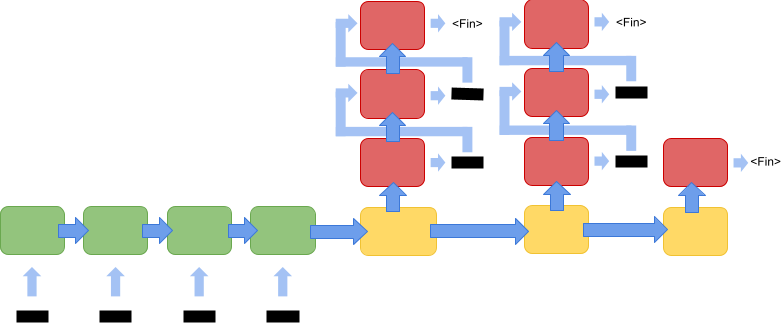
\includegraphics[scale=0.5]{2_production_mots_cles/exhird.png}
    \caption{Représentation schématique du décodage hiérarchique de la méthode ExHirD. L'encodeur du document est représenté en vert, le décodeur de concept en jaune et le décodeur de mots-clés en rouge.}
    \label{fig:schema_exhird}
\end{figure}

Dans le but de mieux modéliser les ensembles de mots-clés, \citet{chen_exclusive_2020} s'intéressent à la structure hiérarchique des ensembles de mots-clés.
En effet, les méthodes de génération de séquences de mots-clés identifient les mots-clés grâce à des marqueurs générés par le modèle. Cette séquentialité ne permet pas de représenter la hiérarchie entre les mots-clés et les mots qui les composent.
Ces travaux se rapprochent de \citet{yuan_generating_2018} qui essaient de rompre la séquentialité en modifiant la représentation des séparateurs de mots-clés avec le mécanisme de régularisation orthogonale.
Ainsi, ils présentent la méthode ExHirD~\cite{chen_exclusive_2020} dans laquelle le décodeur de l'architecture de CopyRNN est remplacé par un décodeur hiérarchique (voir figure~\ref{fig:schema_exhird}) qui génère les mots-clés en deux temps: d'abord l'identification des concepts, ensuite la génération de leur représentation textuelle.
Ce décodeur hiérarchique comprend un premier décodeur qui produit une représentation dense d'un concept, puis un second décodeur qui va générer une séquence de mots à partir de cette représentation dense pour instancier le concept en un mot-clé.
La génération des mots utilise deux mécanismes d'attention sur les documents d'entrée: l'un est conditionné par la représentation dense du concept; l'autre, standard, est conditionné par le mot précédent.
Ainsi, ce décodeur hiérarchique permet de modéliser explicitement les concepts importants du document et les mots qui les décrivent.
%
L'évaluation de cette méthode montre néanmoins un faible gain de performance, de l'ordre d'un point de F@5, pour les mots-clés présents et absents.
%
Ces travaux s'attellent aussi au problème de redondance des mots-clés et proposent un mécanisme de décodage exclusif pour tenter de le résoudre.
Ce mécanisme, simple dans son idée, interdit au modèle de générer deux mots-clés commençant par le même mot.
En effet, les mots-clés comportent le plus souvent entre 1 et 4 mots (voir section~\ref{sub:nature_linguistique}), ainsi le premier mot affecte grandement les suivants.
Ce mécanisme n'est pas limité à la méthode ExHirD; il peut être adapté aux différents types de décodage ou être utilisé en post-traitement.
Son évaluation montre qu'il fait significativement baisser le nombre de mots-clés dupliqués sans faire baisser les scores de F@5.

Les méthodes génératives \emph{one2many} apprennent à déterminer le nombre de mots-clés à produire mais en génèrent trop peu: catSeqD génère en moyenne 4,3 mots-clés par document alors que la référence en est composée de 5,3 en moyenne.
Les travaux de \citet{chan_neural_2019} s'intéressent à encourager les modèles à générer plus de mots-clés, en les entraînant à optimiser le rappel et la \fmesure{}.
Or ces métriques ne peuvent être utilisées comme fonction de coût dans l'algorithme de descente de gradient, car elles ne sont pas dérivables.
Pour résoudre ce problème, les auteurs proposent d'utiliser l'apprentissage par renforcement pour affiner\footnote{\foreign{To fine-tune} en anglais.} des modèles déjà entraînés.
%
Dans l'apprentissage par renforcement~\cite{williams_simple_1992}, un agent produit une série d'actions en suivant une politique (ici la génération de mots grâce à un modèle génératif), puis est récompensé pour chacune des actions.
%Dans l'apprentissage par renforcement~\cite{williams_simple_1992}, un agent produit une série d'actions en suivant une politique puis il est récompensé pour chaque action.
%Dans notre cas, une action consiste à générer un mot, la politique permettant de choisir le mot est un modèle génératif, et la récompense est le rappel ou la f-mesure.
L'algorithme d'apprentissage par renforcement optimise ainsi les poids du modèle (met à jour la politique) en fonction de la récompense.
%
Dans la méthode proposée, la récompense s'adapte selon le nombre de mots-clés générés: s'il est trop faible, la récompense sera le rappel pour encourager le modèle à générer plus de mots-clés; à l'inverse s'il est trop grand, la récompense sera la \fmesure{}, pour encourager le modèle à générer seulement de bons mots-clés.
%
De plus, les mots-clés présents et absents sont récompensés séparément pour favoriser la génération des mots-clés absents.

%CDKGen~\cite{diao_keyphrase_2020} (use close docs to encode, transformers)
%SenseNet~\cite{luo_sensenet_2020} (??)

Les travaux, concernant les méthodes neuronales, présentés jusqu'à présent considèrent que la quantité de données disponibles est suffisante.
Nous verrons dans le chapitre~\ref{chap:framework} que les sources de données contenant des documents annotés en mots-clés sont peu nombreuses malgré la large disponibilité de documents scientifiques en ligne.
Ainsi, les travaux de \citet{ye_semi-supervised_2018} se placent dans un cadre où la quantité de documents annotés est limitée.
%
Pour cela, les auteurs proposent deux méthodes qui tirent parti de la masse de documents non annotés pour la génération de mots-clés.
%
La première méthode consiste à utiliser des documents non annotés en mots-clés dans le cadre d'apprentissage multitâche.
Un réseau de neurones encodeur-décodeur est entraîné, pour les documents annotés, à générer des séquences de mots-clés et, pour les documents non annotés, à générer le titre du document. Dans le modèle, deux décodeurs différents sont utilisés pour chacune des tâches mais l'encodeur est partagé.
%
La seconde méthode consiste à créer un corpus synthétique en annotant automatiquement des documents en mots-clés. Les mots-clés sont extraits grâce aux méthodes \tfidf{} et TextRank.
Ainsi, un modèle de génération de mots-clés est pré-entraîné grâce à la combinaison des corpus synthétique et annoté, puis affiné grâce au seul corpus annoté.
%
L'évaluation des deux modèles résultant de ces méthodes d'entraînement montre qu'ils obtiennent des résultats similaires.
Les scores de F@5 pour les mots-clés présents des modèles semi-supervisés sont comparables à ceux du modèle \emph{catSeq} (CopyRNN entraîné à générer des séquences de mots-clés), bien qu'ils n'utilisent qu'un dixième des documents annotés utilisés par \emph{catSeq}.

\subsection{Extraction de mots-clés}

% Chapeau
Les méthodes génératives de bout-en-bout sont très performantes pour produire des mots-clés présents, mais génèrent très peu de mots-clés absents.
Ainsi, la communauté scientifique s'intéresse à des méthodes de bout-en-bout exclusivement extractives.
%Les méthodes génératives de bout-en-bout sont très performantes pour produire des mots-clés présents, ainsi la communauté scientifique s'intéresse à 
%Les méthodes génératives de bout-en-bout, qui ont la particularité de produire des mots-clés absents, n'en produisent au final que très peu~\cite[inter alia]{chen_exclusive_2020, santosh_hicova_2021} et ceux-ci ne correspondent que très peu aux mots-clés de référence~\cite[inter alia]{ahmad_select_2020, ye_one2set_2021}.
%Mais leurs performances élevées pour produire des mots-clés présents encouragent tout de même le développement de méthodes de bout-en-bout.
%C'est pourquoi la communauté scientifique s'intéresse aux méthodes de bout-en-bout exclusivement extractives.
%
Bien qu'elles ne soient pas au c\oe{}ur de nos travaux, nous présentons les principales méthodes extractives par soucis d'exhaustivité.
% Plan
Dans cette section nous présentons tout d'abord les méthodes fondées sur l'annotation en séquence, ensuite, une méthode de classification, et enfin, une méthode fondée sur les graphes.

Le développement de ces méthodes est lié à celui des modèles de langues pré-entraînés tels que BERT~\cite{devlin_bert_2019}, SciBERT~\cite{beltagy_scibert_2019} ou encore GPT-2~\cite{radford_language_2019} qui reposent sur l'architecture transformer~\cite{vaswani_attention_2017}.
Ils sont utilisés pour fournir des plongements de mots contextuels ou bien pour être affinés pour une tâche particulière.
Ces modèles, entraînés sur de très grandes quantités de données, ont permis d'améliorer significativement les performances de nombreuses tâches de traitement automatique de la langue~\cite{wang_glue_2018}.

% Annotation en séquence
\paragraph{Annotation en séquence}
La grande majorité des méthodes extractives de bout-en-bout reformulent la tâche de production de mots-clés en une tâche d'annotation en séquence.
Dans l'annotation en séquence, chaque mot du document est associé à une étiquette selon un schéma binaire: mot-clé ou non mot-clé, ou bien selon le schéma \texttt{BIO} dans lequel les mots du document correspondent au début (\texttt{B}), à l'intérieur (\texttt{I}) ou à l'extérieur (\texttt{O}) d'un mot-clé.\\
%
La méthode pionnière, proposée par \citet{augenstein_multi-task_2017}, utilise un encodeur récurrent bi-directionnel pour représenter chacun des mots et prédire leurs étiquettes.
Elle est amélioré par \citet{alzaidy_bi-lstm-crf_2019} qui ajoute un champ aléatoire conditionnel (CRF) pour améliorer la prédiction séquentielle des étiquettes, ainsi que par \citet{sahrawat_keyphrase_2019} qui utilise les plongements contextuels de BERT en entrée de l'encodeur.
%
La méthode SaSaKe~\cite{santosh_sasake_2020}, quant à elle, utilise les relations de dépendances syntaxique et sémantique du document pour améliorer la représentation des mots.
Le document est encodé puis les relations de dépendances sont représentées sous formes de graphes et incorporées aux représentations des mots grâce à des réseaux à convolution de graphes.
Ces représentation servent ensuite à étiqueter chaque mot comme mot-clé ou non mot-clé.
%La méthode pionnière, proposée par \citet{augenstein_multi-task_2017}, utilise un encodeur récurrent bi-directionnel pour représenter chacun des mots et prédire leurs étiquettes. D'autres travaux améliorent cette méthode, notamment BiLSTM-CRF~\cite{alzaidy_bi-lstm-crf_2019} qui ajoute à l'encodeur un champ aléatoire conditionnel (CRF), ce qui améliore la prédiction séquentielle des étiquettes. Dans la même ligne de recherche, \citet{sahrawat_keyphrase_2019} améliore BiLSTM-CRF en utilisant les plongements de mots contextuels de BERT en entrée de l'encodeur.\\
%
%D'autres méthodes pour l'annotation en séquence sont présentées, la méthode SaSaKe~\cite{santosh_sasake_2020} par exemple, prend explicitement en compte la syntaxe et la sémantique des documents grâce à leurs graphes de dépendances syntaxique et sémantique. Cette méthode encode le document grâce à un transformer puis incorpore à la représentation de chaque mot les informations des graphes de dépendances à l'aide de réseaux à convolution de graphe.\\
%
%De son côté, \citet{martinc_tnt-kid_2020} propose la méthode TNT-KID qui tire parti du transfert de connaissances d'un modèle de langue pré-entraîné et se place dans un contexte de données limitées. Cette méthode consiste d'abord à pré-entraîner un modèle de langue transformer à l'aide de données non annotées. Puis à affiner ce modèle grâce au seul ensemble de validation de KP20k pour l'identification de mots-clés grâce à l'annotation en séquence. Ainsi, avec seulement \num{20000} documents annotés cette méthode obtient des résultats comparables à ceux de CopyRNN.

% Classification
\paragraph{Classification}
La méthode BERT-JointKPE~\cite{sun_joint_2020} s'inspire des méthodes en chaîne de traitement pour entraîner un modèle de bout-en-bout à classifier chaque n-gramme du document comme mot-clé ou non mot-clé. Cette méthode ressemble donc à une sélection de mots-clés candidats n-grammes (voir section~\ref{selection-des-mots-cles-candidats}).
Les plongements des mots du document sont d'abord calculés à l'aide de BERT. Ensuite, grâce à des convolutions de différentes tailles, les représentations des mots sont agrégées pour représenter les n-gramme (de 1 à 5).
Enfin, chaque n-gramme est classifié comme mot-clé ou non mot-clé grâce à sa représentation dense.

% Enfin
\paragraph{Graphe}
La méthode DivGraphPointer~\cite{sun_divgraphpointer_2019} diffère des autres méthodes extractives car elle est fondée sur le paradigme encodeur-décodeur.
Nous la décrivons en détail pour comparer son architecture à celles des méthodes génératives décrites dans les sections~\ref{sub:generation_de_mots_cles} et \ref{sub:generation_de_sequences_de_mots_cles}.
%
Cette méthode combine la représentation sous forme de graphe, largement utilisée par les méthodes en chaîne de traitement (voir section~\ref{graphe}), et la génération de mots-clés en séquence (\emph{one2many}).%
\footnote{Cette méthode est générative, mais ne peut produire de mots-clés absents. En dehors de sa description nous réservons le terme \say{méthodes génératives} aux seules méthodes pouvant produire des mots-clés absents.}
L'intérêt de cette représentation est double: elle permet premièrement de mutualiser l'information des multiples occurrences d'un même mot; et deuxièmement, elle permet de prendre en compte les interactions entre les mots de manière globale.
%
Ainsi, le document est d'abord représenté sous forme de graphe dans lequel les n\oe{}uds représentent les mots et les arêtes la distance entre les positions des mots.
Ensuite, des couches de convolution de graphe calculent la représentation de chaque n\oe{}ud en fonction de ses voisins.
Ces représentations sont agrégées pour initialiser le décodeur, un \foreign{pointer network}~\cite{vinyals_order_2016}.
Enfin, ce décodeur produit une séquence de mot exclusivement copiée du document.
%
DivGraphPointer à pour objectif, comme \emph{catSeqD}, de produire des mots-clés peu redondants.
Ainsi, en plus du mécanisme d'attention et de couverture, le mécanisme de \emph{modification du contexte} (similaire dans son objectif à la \emph{régularisation orthogonale} de \emph{catSeqD}) recalcule l'état caché après avoir généré un séparateur de mot-clé.
Cet état caché est calculé en fonction de la représentation du document et de l'ensemble des mots-clés précédemment générés.\\
%
Un intérêt peu discuté de cette méthode est sa capacité à produire des mots-clés qui ne sont pas des sous-séquences du document mais dont tous les mots y apparaissent.
Ainsi, la dichotomie entre mots-clés présents et mots-clés absents ne semble ne pas convenir à ce type de mots-clés.
Nous discuterons la définition de mots-clés présents et de mots-clés absents dans le chapitre~\ref{chap:ri}.


\section{Conclusion}

% Méthodes en ch de traitement
%Nous avons vu dans le chapitre~\ref{chap:concepts} les méthodes de production automatique de mots-clés en chaîne de traitement.
%La communauté scientifique à proposé de nombreuses méthodes en chaîne de traitement qui utilisent différents descripteurs pour identifier les mots-clés les plus importants des documents.
%Ces méthodes nécessitent peu de données d'entraînement ou sont non supervisées.
%Elles ne dépendent généralement pas de la langue et peuvent être transposées simplement.
%
%Malheureusement, l'enchaînement des différentes étapes propage et intensifie les erreurs.
%De plus, la définition manuelle des descripteurs, qui nécessite des connaissances expertes, limite la transférabilité des méthodes à d'autres types de document.
%Enfin, ces méthodes en chaîne de traitement, majoritairement extractives, ne peuvent produire que des mots-clés qui sont présents dans le document.
%
%Pour pallier la propagation d'erreurs et la définition manuelle des descripteurs, des méthodes d'apprentissage profond de bout-en-bout sont proposées.
%Malgré leurs avantages, ces méthodes nécessitent d'être entraînées à l'aide de grandes quantités de données annotées.
%
%Ces méthodes sont cependant moins généralisables à d'autres genres de documents de par leur nature supervisée, ainsi qu'à d'autres langues car elles nécessitent des données annotées.
%
%De plus, leur complexité, leur variabilité dans leurs implémentations, leur temps d'exécution et d'entraînement sont aussi des limites à leur utilisation à grande échelle.
%paramètres à prendre en compte en fonction de l'utilisation qui en sera faite.

Dans ce chapitre, nous avons présenté les principes fondamentaux des réseaux de neurones ainsi que le paradigme encodeur-décodeur qui permet d'encoder un document de longueur variable et de générer une séquence de mots.
Nous avons ensuite présenté un état de l'art des méthodes de production de mots-clés de bout-en-bout, toutes neuronales, qui reposent à minima sur les encodeurs ou les décodeurs.
Pour cet état de l'art, nous avons séparé ces méthodes en deux catégories~: les méthodes génératives et les méthodes extractives.


% 2.1 fondements
% 2.1.1 neural nets
% 2.1.2 encodage
% 2.1.3 décodage
% 2.1.4 stratégies de décodages
% 2.1.5 encodeur-décodeur

La mise à disposition, par \citet{meng_deep_2017}, d'une grande quantité de données annotées permet le développement de méthodes de bout-en-bout pour la production de mots-clés.
Ces méthodes de bout-en-bout pallient certains écueils des méthodes en chaîne de traitement, présentées au chapitre~\ref{chap:concepts}, notamment la propagation des erreurs entre les différentes étapes et la définition manuelle des traits pour identifier l'importance des mots-clés.
%
Néanmoins, les méthodes de bout-en-bout ne sont pas exemptes de limites~: elles nécessitent de grandes quantités de données pour être entraînées ainsi qu'une grande puissance de calcul pour être utilisées.
%Elles introduisent néanmoins de nouvelles limitations: premièrement, la nécessité de disposer de grandes quantités de données annotées pour leur entraînement et deuxièmement, la disposition d'une grande puissance de calcul nécessaire à leur exécution.

Les méthodes extractives de bout-en-bout s'inspirent, pour la majorité, de l'annotation en séquence et entraînent des réseaux de neurones à identifier le début et la fin des mots-clés dans les documents.
Ces méthodes sont, de manière générale, plus performantes que les méthodes génératives, ainsi, la spécialisation des méthodes dans l'extraction de mots-clés semble faciliter la tâche.

%Les méthodes génératives, qui constituent le c\oe{}ur de nos travaux, entraînent un réseau de neurones à générer les mots-clés de référence.
%Ces méthodes ont la capacité de produire des mots-clés absents, ce que les méthodes proposées jusqu'alors ne permettaient pas.
%Cependant, l'analyse des mots-clés générés par ces méthodes montre que les mots-clés qui correspondent à la référence sont presque exclusivement des mots-clés présents.
%Ainsi, elles ne produisent en fait que très peu de mots-clés absents et ceux-ci ne correspondent que très peu à la référence.
%Nous verrons dans le chapitre~\ref{chap:ri} que ces mots-clés absents sont un enjeu important pour la tâche de recherche d'information.

Les méthodes génératives, qui constituent le c\oe{}ur de nos travaux, entraînent un réseau de neurones à générer les mots-clés de référence.
Elles ont la capacité de produire des mots-clés absents, ce que les méthodes proposées jusqu'alors ne permettaient pas.
Ces méthodes ont deux principales faiblesses: elles produisent très peu de mots-clés absents (1,7 en moyenne~\cite{chan_neural_2019}) et produisent des mots-clés très redondants (entre  \npercent{20} et \npercent{30}~\cite{chen_exclusive_2020}).
%
Ainsi, les différentes méthodes présentées ont pour objectif de pallier au moins une de ces faiblesses en ajoutant des mécanismes de diversification des mots-clés, en essayant d'améliorer la modélisation des documents ou en modifiant le processus de décodage.
De manière globale, les performances de la tâche de production automatique de mots-clés augmentent peu.
Notons tout de même l'amélioration des performances pour les mots-clés \emph{présents} de 33 à 40 points de F@5 sur KP20k entre les premiers travaux de \citet{meng_deep_2017} et ceux, plus récents, de \citet{ye_heterogeneous_2021}.
%La production de mots-clés présents augmente tout de même: les premiers travaux de \citet{meng_deep_2017} et ceux, plus récents, de \citet{ye_heterogeneous_2021} rapportent respectivement une F@5 sur KP20k de 33 et de 40 points.
%Mais la production de mots-clés absents, elle, stagne: \citet{chan_neural_2019} et \cite{ye_heterogeneous_2021} rapportent respectivement une F@5 sur KP20k de 1,5 et 3.
Mais, malgré cette augmentation de performance pour les mots-clés présents, les performances pour les mots-clés \emph{absents} ne dépassent pas 5 points de F@5~\cite{chan_neural_2019,ye_heterogeneous_2021}.
%
Nous verrons dans le chapitre~\ref{chap:ri} que ces mots-clés absents sont un enjeu important pour la tâche de recherche d'information.


%Premièrement, elles produisent très peu de mots-clés absents (1,7 en moyenne contre 3,9 pour les mots-clés présents ~\cite{chan_neural_2019}) et ceux-ci ne correspondent que très peu à la référence (avec une F@5 maximale de 3,6 atteinte par \citet{ye_one2set_2021}).
%Deuxièmement, les mots-clés générés sont très redondants, ceux-ci prennent la place de bon mots-clés possible \citet{chen_exclusive_2020} estime qu'entre \npercent{20} et \npercent{30} des mots-clés produits sont redondants.


%Les principaux problèmes des méthodes générative sont que les mots-clés produits sont très redondants, et que très peu de mots-clés absents sont effectivement généré (qu'ils correspondent à la référence ou pas).
%Ainsi les différentes méthodes présentées ont pour objectif de pallier l'un de ces problèmes en ajoutant des mécanisme ou en modifiant le processus d'entraînement des modèles.
%Les améliorations en terme de \fmesure{} de chaque méthode sont peu significatives.
%
%Les méthodes d'annotation en séquence, quant à elles, sont de manière générales plus performantes que les méthodes génératives.
%Ainsi, la spécialisation des méthodes dans l'extraction de mots-clés semble faciliter la tâche.
%Elles obtiennent, sur KP20k, des scores de l'ordre de 45 points de \fmesure{} pour les mots-clés présents, ce qui est supérieur aux méthodes génératives qui, pour l'instant, obtiennent des scores toujours inférieurs à 40 points de \fmesure{}.

\cleardoublepage
\chapter{Production de mots-clés de bout-en-bout} \label{chap:kw_production}

Ce chapitre présente les méthodes de production de mots-clés de l'état de l'art de bout-en-bout, qui constituent l'élément principal de ce travail de thèse. 
Nous commencerons par présenter les composants de ces méthodes auxquels nous feront référence dans la partie état de l'art.

\section{Principes fondamentaux des réseaux de neurones}
% Fondements sur les réseaux de neurones

Nous présentons dans cette section les concepts nécessaires à la bonne compréhension des méthodes de production de mots-clés de bout-en-bout.
Nous décrivons d'abord en détail les réseaux de neurones, ensuite les plongements de mots (\foreign{word embeddings}) utilisés pour représenter les mots du langage naturel, et enfin le paradigme encodeur-décodeur qui permet de traiter du texte de longueur variable en entrée et en sortie des réseaux de neurones.

Contrairement aux méthodes en chaîne de traitement décrites dans la section~\ref{sec:methode-en-chaine-de-traitement}, les méthodes de bout-en-bout, qui utilisent le paradigme encodeur-décodeur, se passent de l'identification des candidats ainsi que du choix des caractéristiques des mots-clés qui serviront à les pondérer.
En effet, les méthodes que nous décrivons dans ce chapitre utilisent des réseaux de neurones profonds qui apprennent à extraire automatiquement les descripteurs  les plus pertinents.
%L'apprentissage profond, permet de laisser le modèle extraire les descripteurs de manière automatique au lieu de les définir à la main, ce qui nécessite des connaissances expertes. Mais cela est difficile à interpreter, tout un pan de la recherche s'intéresse à expliquer ces méthodes (blackbox nlp)~\cite{}.


\subsection{Réseaux de neurones}
\label{sub:neural_network}

\begin{figure}
    \centering
    %Heavily inspired from https://texample.net/tikz/examples/neural-network/

\begin{tikzpicture}[shorten >=1pt,->,draw=black!50]
    \def\myscale{1.5}
    \tikzstyle{neuron}=[circle,fill=black!25,minimum size=17*\myscale,inner sep=0cm]
    \tikzstyle{input neuron}=[neuron, fill=color1!60];
    \tikzstyle{hidden neuron}=[neuron, fill=color0!60];
    \tikzstyle{output neuron}=[neuron, fill=color2!60];
    \tikzstyle{edge label}=[above=-.025cm,sloped,scale=.4*\myscale,black!60]
    \tikzstyle{label}=[scale=.75*\myscale, text width=2cm, align=center]

    \def\layersep{2.5*\myscale}
    \def\ninput{2}
    \def\nlayerone{3}
    \def\nlayertwo{2}
    \def\noutput{2}

    % Draw the input layer nodes
    \foreach \name / \y in {1,...,\ninput}
    % This is the same as writing \foreach \name / \y in {1/1,2/2,3/3,4/4}
        \node[input neuron] (I-\name) at (0,-\y*\myscale) {};


    % Draw the hidden layer nodes
    \foreach \name / \y in {1,...,\nlayerone}
        \path[yshift=.5*\myscale cm]
            node[hidden neuron] (H1-\name) at (1*\layersep,-\y*\myscale) {};

    \foreach \name / \y in {1,...,\nlayertwo}
        \path[yshift=.0*\myscale cm]
            node[hidden neuron] (H2-\name) at (2*\layersep,-\y*\myscale) {};

    % Draw the output layer node
    \foreach \name / \y in {1,...,\noutput}
        \path[yshift=0*\myscale cm]
            node [output neuron] (O-\name) at (3*\layersep,-\y*\myscale) {};

    % Connect every node in the input layer with every node in the
    % hidden layer.
    
    %\foreach \source in {1,...,\ninput}
    %    \foreach \dest in {1,...,\nlayerone}
    %        \draw[->] (I-\source) -- node [edge label, pos={.28-}] {$W^1_{\source,\dest}$} (H1-\dest);
    
    \def\layerout{1}
    \def\source{1}
    \foreach \dest / \n in {1/.2,2/.25,3/.235}
        \draw[->] (I-\source) -- node [edge label, pos={\n}] {$W^\layerout_{\source,\dest}$} (H\layerout-\dest);
    \def\source{2}
    \foreach \dest / \n in {1/.17,2/.285,3/.26}
        \draw[->] (I-\source) -- node [edge label, pos={\n}] {$W^\layerout_{\source,\dest}$} (H\layerout-\dest);


    \def\layerout{2} % modify this
    \pgfmathtruncatemacro{\layerin}{\layerout - 1}
    \def\source{1} % modify this
    \foreach \dest / \n in {1/.2,2/.26} % modify this
        \draw[->] (H\layerin-\source) -- node [edge label, pos={\n}] {$W^\layerout_{\source,\dest}$} (H\layerout-\dest);
    \def\source{2} % modify this
    \foreach \dest / \n in {1/.2,2/.25} % modify this
        \draw[->] (H\layerin-\source) -- node [edge label, pos={\n}] {$W^\layerout_{\source,\dest}$} (H\layerout-\dest);
    \def\source{3} % modify this
    \foreach \dest / \n in {1/.23,2/.3} % modify this
        \draw[->] (H\layerin-\source) -- node [edge label, pos={\n}] {$W^\layerout_{\source,\dest}$} (H\layerout-\dest);

    % Connect every node in the hidden layer with the output layer
    \def\layerout{3} % modify this
    \pgfmathtruncatemacro{\layerin}{\layerout - 1}
    \foreach \source in {1,...,\nlayertwo}
        \foreach \dest in {1,...,\noutput}
            \draw[->] (H\layerin-\source) -- node [edge label, pos={.20+(1-Mod(\dest,2))*.05}] {$W^\layerout_{\source,\dest}$} (O-\dest);

    % Annotate the layers
    \node[label, below=.1cm of I-\ninput] (I-label) {Entrée};

    \node[draw, dashed, rounded corners,fill=none, fit=(H1-1) (H1-\nlayerone)] (H1) {};
    \node[label, below=.1cm of H1] (H1-label) {Première couche};

    \node[draw, dashed, rounded corners,fill=none, fit=(H2-1) (H2-\nlayertwo)] (H2) {};
    \node[label, below=.1cm of H2] (H2-label) {Seconde couche};

    \node[draw, dashed, rounded corners,fill=none, fit=(O-1) (O-\noutput)] (O) {};
    \node[label, below=.1cm of O] (O-label) {Couche de sortie};

    \node[draw, dashed, rounded corners,fill=none, fit=(H1) (H1-label) (H2) (H2-label)] (H) {};
    \node[label, text width=10cm, below=.1cm of H] (H-label) {Couches cachées};

\end{tikzpicture}
    \caption{Représentation graphique d'un réseau de neurones à 2 couches. Les flèches représentent les poids des matrices $W^k$. Les biais $b^k$ ne sont pas représentés.}
    \label{fig:ex_nn_simple}
\end{figure}
% https://texample.net/tikz/examples/neural-network/

Les réseaux de neurones servent à modéliser des fonctions complexes, qui peuvent être non linéaires.
%
D'un point de vue mathématique, il s'agit de modéliser une fonction $f$ qui prend une entrée $X$ et retourne une sortie (une prédiction) $\hat{Y} = f(X)$.
%
Ici, $X \in M_{1,m}(\mathds{R})$ et $\hat{Y} \in M_{1,n}(\mathds{R})$ sont des vecteurs de taille $m$ et $n$ respectivement.
%
Ces vecteurs représentent le nombre de paramètres d'entrée de la fonction $f$.
%
%Par exemple, un modèle qui prédit le prix d'une maison en fonction de sa surface et du nombre de fenêtres aura 2 entrées et une sortie.


Un réseau de neurones simple (également appelé perceptron mono-couche) est défini par l'équation~\ref{eq:simple_nn} ci-dessous, dans laquelle $W$ est une matrice de poids $W \in M_{m, n}(\mathds{R})$ et $b$ un vecteur de biais $b \in M_{1,m}(\mathds{R})$.
%
\begin{align}
    \hat{Y} = f(X) = \sigma (b + W * X) \label{eq:simple_nn}
\end{align}


La fonction $\sigma$ est une fonction dite d'activation.
Elle est inspirée de l'activation des neurones dans le cerveau humain.
L'information d'un neurone passe à la couche suivante si le neurone est activé (c'est-à-dire si sa valeur est assez élevée).
Les fonctions Sigmoïde (voir équation~\ref{eq:sigmoide}) et Rectified Linear Unit (ReLU) (voir équation~\ref{eq:relu}) sont généralement utilisées pour $\sigma$.
%Cette fonction est généralement la fonction sigmoïde (équation~\ref{eq:sigmoide}), Rectified Linear Unit (ReLU) (équation~\ref{eq:relu}), ou tangente hyperbolique ($\text{tanh}$). \todo{comment choisir cette fonction ?}

\begin{gather}
    \sigma(x) = \frac{1}{1+e^{-x}} \label{eq:sigmoide} \\
    \textsc{ReLu}(x) = \text{max}(0, x) \label{eq:relu}
\end{gather}

%\begin{figure}\centering
%    \begin{tikzpicture}\begin{axis}[xmin=-5, xmax=5, ymin=-2, ymax=2]
%        \addplot {1/(1+e^(-x))};
%        \addplot {tanh(x)};
%        \addplot {max(x, 0};
%    \end{axis}\end{tikzpicture}
%    \caption{Caption} \label{fig:my_label}
%\end{figure}

Un réseau de neurones à une couche (perceptron mono-couche) ne peut modéliser que des fonctions linéaires, et ne pourra jamais modéliser une fonction telle que la fonction XOR par exemple~\cite{minsky_perceptrons_1988}.
Pour gagner en expressivité, des couches de neurones sont ajoutées (voir figure~\ref{fig:ex_nn_simple}). Un tel réseau de neurones est aussi appelé perceptron multicouche.
%
Un perceptron mono ou multicouche dénote un réseau de neurones à propagation avant (\foreign{feed forward neural network}) où chaque couche est entièrement connectée à la suivante.

En utilisant les perceptrons multicouche, il est possible de modéliser des fonctions plus complexes.
Dans ce cas, chaque couche utilise la sortie de la couche précédente comme entrée (voir équation~\ref{eq:multi_nn}).
La couche \num{0} représente l'entrée du réseau, $k$ représente une couche intermédiaire et $n$ la couche de sortie.
Les matrices $W$ (et leur vecteurs de biais) définissent la taille de chaque couche (c'est-à-dire le nombre de neurones).
En effet, une matrice de taille $n*m$ (et un vecteur $b$ de taille $m$) définit une couche de taille $m$, $n$ étant conditionné par la taille de la couche précédente.
%
\begin{equation}\label{eq:multi_nn}
  \begin{split}
    h^0 & = X \\
    h^k & = \sigma(b^k + W^k * h^{k-1}) \\
    \hat{Y} & = h^n
  \end{split}
\end{equation}

Entraîner le réseau de neurones $f$ consiste à modifier les paramètres du modèle $\theta$ (matrices de poids $W^k$ et $b^k$) afin de minimiser l'erreur de prédiction. Cette erreur est définie par une fonction de coût (\emph{loss function}) $\mathcal{L}$ (voir équation~\ref{eq:loss}) calculé grâce à une prédiction $\hat{Y} = f(X)$ et une vérité terrain $Y$.
Le but de l'entraînement est de minimiser cette fonction de coût pour tous les exemples d'un jeu de données, dénoté par l'équation~\ref{eq:loss_dataset}.
%
\begin{gather} 
    \text{erreur} = \mathcal{L}(\hat{Y}, Y) = \mathcal{L}(f(X, \theta), Y) \label{eq:loss} \\
    \text{min}_\theta \sum_{(x, y) \in \mathcal{D}} \mathcal{L}(f(x, \theta), y) \label{eq:loss_dataset}
\end{gather}

L'algorithme utilisé pour minimiser la fonction de coût dans le cadre des réseaux de neurones est la descente de gradient~\cite{curry_method_1944} (Gradient Descent).
Le gradient de la fonction de coût donne la direction dans laquelle modifier les paramètres (ici les poids du réseau de neurones) pour minimiser ce coût.
Cet algorithme calcule le gradient avec tous les exemples du jeu de données puis met à jour les poids du réseau; ce processus est donc très long. Pour pallier cette lenteur, la descente de gradient par minibatch calcule le gradient à l'aide d'un nombre fixe d'exemples qui fait un compromis entre temps de calcul et utilisation d'un grand nombre d'exemples.
% figure 
%Cet algorithme utilise le fait que la fonction de coût et le réseau de neurones soient dérivables pour calculer le gradient de l'erreur et modifier les poids par rétro-propagation pour minimiser l'erreur.

Les réseaux de neurones que nous venons de décrire fonctionnent avec une entrée de taille fixe $X$; or dans le cas du texte, les entrées sont des séquences de mots de longueur variable, et n'ont donc pas de longueur fixe. Nous présentons dans la suite de cette section une architecture permettant de traiter les entrées de longueur variable.

\subsection{Encodage de séquences (encodeur)}
\label{sub:encoding}

\subsubsection{Représentation dense des mots}
\label{sec:word_embedding}

Les réseaux de neurones manipulent des vecteurs et des matrices de nombres. Le langage naturel étant constitué par des mots, il est nécessaire de transformer les mots en nombres.
Pour cela, un vocabulaire qui associe un nombre à chacun des mots est nécessaire. La méthode la plus simple est de considérer les mots les plus fréquents d'un ensemble de documents d'entraînement comme le vocabulaire $\mathcal{V}$.
Un vocabulaire de taille trop importante peut être difficile à modéliser et contiendra de nombreux hapax\footnote{Mots n'apparaissant qu'une seule fois.}. Il est donc courant de conserver les \num{50 000} mots les plus fréquents~\cite{meng_deep_2017,yuan_one_2020,ye_one2set_2021}.
%Plusieurs techniques sont utilisés pour représenter un document sous forme de vecteur à l'aide d'un tel vocabulaire.
%L'encodage \emph{one-hot}, crée un vecteur de la taille du vocabulaire $|\mathcal{V}|$ où chaque dimension représente la fréquence du mot correspondant dans le document. Cette méthode est peu efficiente en terme d'espace car le vecteur ainsi créé est creux (il contient une grande majorité de 0).

% exemple image
Aujourd'hui, les plongements de mots sont l'état de l'art en termes de représentation de mots. Ce sont des représentations denses apprises sur de grandes quantités de données qui modélisent les cooccurrences entre les mots: deux mots utilisés dans des contextes similaires auront des vecteurs similaires~\cite{mikolov_efficient_2013}.
Plusieurs méthodes ont été proposées pour pré-entraîner ces plongements.
Les méthodes précurseures word2vec~\cite{mikolov_efficient_2013} et gloVe~\cite{pennington_glove_2014} calculent des représentations fixes des mots. Leurs principales lacunes sont la prise en compte de mots hors du vocabulaire et la prise en compte de la polysémie. Pour prendre en compte les mots hors du vocabulaire, fastText~\cite{bojanowski_enriching_2017} apprend des plongements de n-grammes de caractères puis combine ceux-ci pour représenter le mot entier. Ensuite, pour traiter la polysémie, Elmo~\cite{peters_deep_2018} et Bert~\cite{devlin_bert_2019} calculent ces plongements en fonction du contexte des mots.
Il est aussi possible d'entraîner des plongements à l'aide d'une simple matrice de poids au début du réseau de neurones. Dans la tâche de génération de mots-clés, cette technique est la plus utilisée.


\subsubsection{Encodeurs}

Les encodeurs sont des réseaux de neurones qui permettent de traiter des séquences de longueur variable. Dans nos travaux ces séquences sont des documents textuels.
Les encodeurs prennent en entrée une séquence de vecteurs, ici des plongements de mots, et donnent en sortie un vecteur de pensée qui agrège l'information de la séquence d'entrée.

Il existe différents types de réseaux permettant d'encoder une séquence: les réseaux récurrents, les réseaux à convolution, les transformers, les réseaux à convolutions de graphes.
Nous nous intéresserons ici aux encodeurs récurrents, les plus utilisés pour la génération de mots-clés. 
Un encodeur récurrent est composé d'une ou plusieurs cellules récurrentes empilées.
Une cellule récurrente $\textsc{Rnn}$ encode une séquence selon l'équation~\ref{eq:rnn}.
%
\begin{equation}\label{eq:rnn}
\begin{split}
    h_t & = \textsc{Rnn}^e(x_{t}, h_{t-1}) \\
    \textsc{Rnn}^e(x_t, h_{t-1}) & = \text{tanh}(W_x * x_t + b_x + W_h * h_{t-1} + b_h)
\end{split}
\end{equation}

Dans l'équation~\ref{eq:rnn} $x_t$ représente le plongement du mot $t$, $h_t$ l'état caché au temps $t$ qui encode la sous-séquence d'entrée jusqu'au mot $t$, $W_x$ et $W_h$ des matrices de poids et $b_x$, $b_h$ les vecteurs de biais correspondants.
Le premier état caché $h_0$ est initialisé aléatoirement.
Ces réseaux sont dits récurrents car l'état caché $h_t$ est conditionné par les états cachés précédents.

Ce type d'encodeurs peut être utilisé pour entraîner un classifieur de documents en utilisant le dernier vecteur $h_t$, par exemple dans le cadre de la catégorisation de documents~\cite{wang_disconnected_2018} ou la détection de rumeurs~\cite{ma_detecting_2016}.
Il est aussi possible d'utiliser ces encodeurs pour entraîner des modèles d'annotation en séquence qui utilisent chaque représentation $h_t$ pour prédire l'étiquette du mot, par exemple dans le cadre de la reconnaissance d'entités nommées~\cite{zukov-gregoric_named_2018}.

% long dependence \todo{parler de ça}
% bidirectionnel
% oubli du début de  la séquence
Le principal écueil des réseaux récurrents est leur difficulté à garder en mémoire les dépendances à long terme.
Pour pallier ce problème, \citet{hochreiter_long_1997}  introduit les cellules LSTM (Long Short Term Memory).
Ces cellules récurrentes contiennent des \say{portes} qui leur permettent d'apprendre à sélectionner les informations à conserver ou à oublier à chaque temps $t$.
Elles donnent en sortie un état caché $h_t$ qui représente l'information pertinente au moment $t$ ainsi qu'un vecteur de contexte $C_t$ qui contient l'ensemble de l'information que la cellule a mémorisé.
Ce mécanisme de portes permet de prendre en compte les dépendances à long terme.
Cette cellule récurrente a été améliorée, notamment par les cellules récurrentes GRU (Gated Recurrent Unit)\cite{cho_learning_2014} qui simplifient les LSTM en combinant $h_t$ et $C_t$ en un unique vecteur ainsi qu'en diminuant le nombre de paramètres utilisés, ce qui en facilite l'entraînement.

Pour améliorer l'encodage des documents et la modélisation des dépendances à long terme, \citet{schuster_bidirectional_1997} présente des encodeurs bi-directionnels.
Ceux-ci sont composés de deux encodeurs qui encodent chacun la séquence dans un sens différent, du début à la fin et inversement.
Chacun de leurs états cachés sont ensuite concaténés pour n'en former qu'un. Ainsi, les états cachés de ce type d'encodeur représentent la séquence entière centrée sur le mot $t$.
%\say{You can't cram the meaning of a whole \%\&\!\$\# sentence into a single \$\&!\#* vector!} (R. Mooney).


\subsection{Génération de séquences (décodeur)}
\label{sub:decoding}

Le processus de décodage permet de générer une séquence de mots à partir d'un vecteur de pensée. Ce vecteur de pensée résulte généralement de l'encodage d'un document (cf. section~\ref{sub:encoding}).
Comme pour l'encodage, différents types de réseaux peuvent être utilisés: les réseaux récurrents, les réseaux à convolutions ou les transformers.
Nous nous intéressons ici aux réseaux récurrents, présentés dans la section~\ref{sub:encoding}.

Un décodeur récurrent est composé d'une ou plusieurs cellules récurrentes empilées.
La génération d'une séquence consiste à utiliser les états cachés $h_t$ pour prédire un mot, c'est-à-dire à produire une distribution de probabilités sur l'ensemble du vocabulaire puis à choisir le mot le plus probable.


Le processus de décodage est décrit par l'équation~\ref{eq:rnn_decodeur} avec $y_{t-1}$ le mot prédit précédemment, $h_{t-1}$ l'état caché précédent, $W_x$ et $W_h$ des matrices de poids et leurs biais correspondant $b_x$ et $b_h$.
Le premier mot $y_0$ est initialisé par un mot spécial; l'état caché $h_0$ est un vecteur de pensée.
Puis $p(y_t | y_{1,...,t-1},h_0)$ représente la distribution de probabilités sur le vocabulaire pour le mot $t$ en fonction des mots précédents et du vecteur de pensée $h_0$; $W_v$ et $b_v$ sont une matrice de poids et son biais.


\begin{equation} \label{eq:rnn_decodeur}
\begin{split}
    p(y_t | y_{1,...,t-1},h_0) & = \textsc{Softmax}(\sigma(W_v * h_t + b_v))\\
    h_t & = \textsc{Rnn}^d(y_{t-1}, h_{t-1}) \\
    \textsc{Rnn}^d(x_t, h_{t-1}) & = \text{tanh}(W_x * x_t + b_x + W_h * h_{t-1} + b_h)
    % p(Y) = \prod p(w_t|w_{t-1},...,w_0,h)
\end{split}
\end{equation}

La génération d'une séquence de mots s'effectue mot-à-mot grâce à un algorithme de décodage.
Chaque étape de décodage consiste à produire une distribution de probabilité sur le vocabulaire de sortie $p(y_t | y_{1,...,t-1},h_0)$ et à choisir un mot $\hat{y}_t$ qui maximise cette probabilité.
Cette étape est répétée jusqu'à ce qu'un mot spécial finissant la séquence soit généré ou que la séquence soit assez longue.

L'algorithme le plus simple consiste à choisir le mot le plus probable à chaque étape mais cela ne permet de générer qu'une seule séquence.
%
Dans le cadre de la génération de mots-clés il est souhaitable de générer plusieurs mots-clés et donc plusieurs séquences.
Pour cela, c'est l'algorithme de recherche en faisceau~\cite{ow_filtered_1988}, que nous schématisons dans la figure~\ref{fig:beam_search}, qui est utilisé.
Cet algorithme consiste à décoder un nombre fixe de séquences (deux dans le schéma).
Les étapes de décodage sont effectuées pour chacun des faisceaux et les mots à générer sont choisis dans l'ensemble des mots des faisceaux.
Dans la figure~\ref{fig:beam_search}, deux mots sont choisis au départ.
Une étape de décodage est ensuite effectuée pour les deux faisceaux.
\`A la troisième étape, le préfixe \texttt{ba} n'est pas conservé car les deux séquences les plus probables sont issues du préfixe \texttt{ab}.
\`A la fin de l'algorithme, deux séquences ont été générées: \texttt{aba} et \texttt{abb}.

\begin{figure}[ht!]
    \centering
    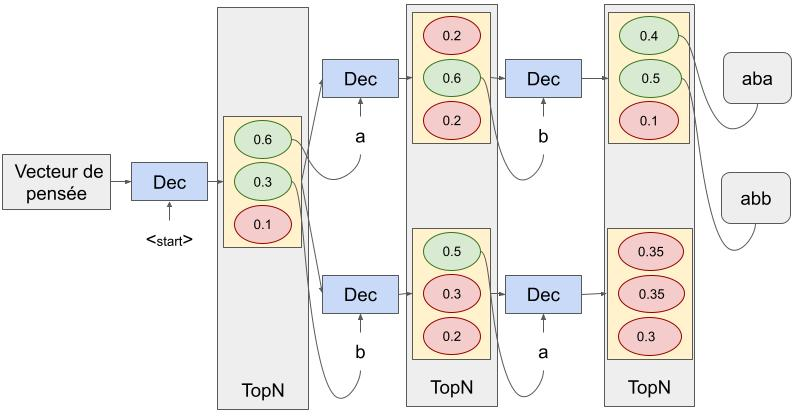
\includegraphics[scale=0.4]{2_production_mots_cles/Beam Search.jpg}
    \caption{Représentation schématique du processus de décodage grâce à l'algorithme de recherche en faisceau.}
    \label{fig:beam_search}
\end{figure}
\todo{refaire en tikz}

\`A l'inverse des algorithmes déterministes que nous avons décrits, notons l'existence des algorithmes d'échantillonnage. Ces algorithmes stochastiques choisissent les mots au hasard en fonction de leur probabilité. Les mots-clés générés par ces algorithmes ne sont donc pas reproductibles, ce qui dans le cadre de la production de mot-clés n'est pas souhaitable. Nous ne considérons donc pas cette technique.

\subsection{Paradigme encodeur-décodeur}\label{sub:paradigme_encodeur_decodeur}

Nous avons présenté dans les sections~\ref{sub:encoding} et \ref{sub:decoding} des moyens d'encoder des documents ainsi que des moyens de générer des séquences.
De nombreuses applications du traitement automatique de la langue nécessitent à la fois l'encodage d'une séquence et son décodage.
Par exemple dans le cadre de la traduction automatique, étant donnée une phrase en langue source, il faut la traduire dans une langue cible, c'est-à-dire qu'il faut encoder la phrase dans la langue source puis générer une phrase correspondante dans la langue cible.
Dans le cadre de la production de mots-clés, il faut générer un mot-clé en fonction d'un document.
Ainsi, le paradigme encodeur-décodeur introduit par \citet{sutskever_sequence_2014}, qui concatène un encodeur et un décodeur, permet de prendre en entrée une séquence de mots de longueur variable et de générer en sortie une autre séquence de mots de longueur variable.
Ce paradigme pallie la limite des réseaux de neurones présentés dans la section~\ref{sub:neural_network} (perceptrons mono ou multicouches) dont l'entrée et la sortie sont de taille fixe.

%Une fois une séquence encodée il est possible de la décoder, c'est-à-dire de produire un mot en fonction d'une représentation $h^t$.
%Générer un mot à partir d'une représentation $h_t$ consiste à passer la représentation dans un perceptron qui calcule une distribution de probabilité sur un vocabulaire, le mot à générer est choisis en fonction de sa probabilité.
    
%\begin{align}
    %\text{log}\: p(y|x) = \sum^m_{j=1} \text{log}\: p(y_j|y_{<j}, x)
%\end{align}

% FROM RECITAL SOTA

\colorlet{enccolor}{green!5}
\colorlet{inputcolor}{black!90!green}
\colorlet{deccolor}{blue!5}
\colorlet{outputcolor}{black!70!blue}
\colorlet{veccolor}{orange!15}
\colorlet{startendcolor}{black!60}
\colorlet{greybox}{black!3}

\begin{figure}[!htb]
\centering

\resizebox{\textwidth}{!}{%
\begin{tikzpicture}

\tikzstyle{cell}=[text centered, rectangle, draw, line width=.5pt, minimum height=1cm, minimum width=1.4cm, rounded corners=2pt]
\tikzstyle{word}=[font=\small\bfseries, text centered, minimum size=.5cm, minimum height=.3cm, text height=1.5ex, text depth=.25ex]
\tikzstyle{vector}=[text centered, rectangle, draw, line width=.5pt, minimum height=.5cm, minimum width=1cm, rounded corners=2pt]
\tikzstyle{arrow}=[shorten >= 2pt, shorten <= 2pt, draw=black!80]

\node[cell, fill=enccolor] (E1) at (0,0){};
\node[cell, fill=enccolor] (E2) at (2,0){};
\node[cell, fill=enccolor] (E3) at (4,0){};
\node[cell, fill=enccolor] (E4) at (6,0){};
\node[text centered] (E5) at (7.5,0){...};
\node[cell, fill=enccolor] (E6) at (9,0){};

\node[word, color=inputcolor, inner color=yellow!50, outer color=white] (I1) at (0,-1.2){Espace};
\node[word, color=inputcolor, inner color=yellow!50, outer color=white] (I2) at (2,-1.2){:};
\node[word, color=inputcolor, inner color=yellow!50, outer color=white] (I3) at (4,-1.2){la};
\node[word, color=inputcolor, inner color=yellow!50, outer color=white] (I4) at (6,-1.2){station};
%\node[word, color=inputcolor, inner color=yellow!50, outer color=white] (I5) at (8,-1.2){...};
\node[word, color=startendcolor] (I6) at (9,-1.2){<fin>};

%\node[cell, fill=veccolor, word, rotate=90] (V) at (11,0){vecteur de pensée};

\node[cell, fill=deccolor] (D1) at (11,0){};
\node[cell, fill=deccolor] (D2) at (13,0){};
\node[cell, fill=deccolor] (D3) at (15,0){};
%\node[cell, fill=deccolor] (D4) at (20,0){};

\node[word, color=startendcolor] (I7) at (11,-1.2){<début>};
\node[word, color=outputcolor, inner color=yellow!50, outer color=white] (O1) at (11,1.2){station};
\node[word, color=outputcolor, inner color=yellow!50, outer color=white] (O2) at (13,1.2){spatiale};
\node[word, color=startendcolor] (O3) at (15,1.2){<fin>};

\draw[->,>=latex,arrow] (E1) -- (E2) node[above,midway] {$h^e_0$};
\draw[->,>=latex,arrow] (E2) -- (E3) node[above,midway] {$h^e_1$};
\draw[->,>=latex,arrow] (E3) -- (E4) node[above,midway] {$h^e_2$};
\draw[->,>=latex,arrow] (E4) -- (E5) node[above,midway] {$h^e_3$};
%\draw[->,>=latex,arrow] (E5) -- (E6) node[above,midway] {$h^e_{n-1}$};
\draw[->,>=latex,arrow] (E5) -- (E6) node[above,midway] {$h^e_{n-1}$};

\draw[->,>=latex,arrow,shorten <= -2pt] (I1) to (E1);
\draw[->,>=latex,arrow,shorten <= -2pt] (I2) to (E2);
\draw[->,>=latex,arrow,shorten <= -2pt] (I3) to (E3);
\draw[->,>=latex,arrow,shorten <= -2pt] (I4) to (E4);
%\draw[->,>=latex,arrow,shorten <= -2pt] (I5) to (E5);
\draw[->,>=latex,arrow,shorten <= -2pt] (I6) to (E6);
\draw[->,>=latex,arrow,shorten <= -2pt] (I7) to (D1);


\draw[->,>=latex, arrow] (E6) -- (D1) node[above,midway] {$h^e_n$};

\draw[->,>=latex,arrow] (D1) -- (D2) node[above,midway] {$h^d_0$};
\draw[->,>=latex,arrow] (D2) -- (D3) node[above,midway] {$h^d_1$};
%\draw[->,>=latex,arrow] (D3) to (D4);

\draw[->,>=latex,arrow,shorten >= -2pt] (D1) to (O1);
\draw[->,>=latex,arrow,shorten >= -2pt] (D2) to (O2);
\draw[->,>=latex,arrow,shorten >= -2pt] (D3) to (O3);
%\draw[->,>=latex,arrow,shorten >= -2pt] (D4) to (O4);

%\node at (5,2) {\large{\textsc{Encodeur}}};
%\node at (17,2) {\large{\textsc{Décodeur}}};

\draw[arrow, rounded corners=3pt] (O1) -| (12, 0);
\draw[->,>=latex, arrow, rounded corners=3pt] (12, 0) -- (12, -1) -| (D2.south);

\draw[arrow, rounded corners=3pt] (O2) -| (14, 0);
\draw[->,>=latex, arrow, rounded corners=3pt] (14, 0) -- (14, -1) -| (D3.south);

%\draw[arrow, rounded corners=3pt] (O3) -| (19, 0);
%\draw[->,>=latex, arrow, rounded corners=3pt] (19, 0) -- (19, -1) -| (D4.south);

\draw[decoration={brace},decorate] (-0.7,1.7) -- node[below=-1.9em] {\large{\textsc{Encodeur}}} (9.7,1.7);
\draw[decoration={brace},decorate] (10.3,1.7) -- node[below=-1.9em] {\large{\textsc{Décodeur}}} (15.7,1.7);


\end{tikzpicture}
}

\caption{Exemple de modèle \textit{encodeur-décodeur} récurrent appliqué à l'extraction automatique de mots-clés.}
\label{fig:seq2seq}
\end{figure}


Le processus d'encodage et de décodage est décrit par l'équation~\ref{eq:enc-dec} et la figure~\ref{fig:seq2seq}.
Dans un premier temps la séquence d'entrée $X$ de taille $n$ est encodée dans le vecteur de pensée $h^e_n$.
Ce vecteur $h^e_n$ est utilisé pour initialiser le premier état caché du décodeur $h^d_0$.
Le décodeur génère ensuite les mots $\hat{y}_t$ qui composent la séquence de sortie $\hat{Y}$ à partir de cet état caché.

\begin{equation}\label{eq:enc-dec}
  \begin{split}
    p(\hat{y}_t | y_{1,...,t-1},h_0) & = \textsc{Softmax}(\sigma(b_v + W_v * h^d_t)) \\
    h^d_t & = \textsc{Rnn}^d(\hat{y}_{t-1}, h^d_{t-1}) \\
    \hat{y}_0 & = \textsc{Debut} \\
    h^d_0 & = h^e_n \\
    h^e_n & = \textsc{Rnn}^e(X) \\
  \end{split}
\end{equation}

Nous présentons ci-après deux améliorations de ce paradigme.
%
D'abord, le mécanisme d'attention qui permet de porter attention à une partie spécifique de l'entrée lors du décodage. Par exemple, la description d'une image nécessite d'identifier les différents objets qui la composent.
%
Ensuite, le mécanisme de copie qui pallie l'incomplétude du vocabulaire de sortie. Ce mécanisme permet au décodeur de copier un mot du document d'entrée au lieu de le générer à partir du vocabulaire de sortie. Le mécanisme de copie est particulièrement utile pour les entités nommées par exemple. Ces entités sont peu fréquentes et ne font généralement pas partie du vocabulaire de sortie.

% Convolution
%Les réseaux de neurones à convolution sont surtout utilisés pour le traitement d'images. Dans le cas du texte, des 
    
% Graphes
%Les réseaux à convolution de graphes (GCN) permettent d'obtenir pour chaque noeud d'un graphe un embedding en fonction de ses voisins. Le nombre de convolutions représente le nombre de bonds qui sont fait entre les noeuds.
    
% Transformer
%Les transformer ont été introduit par \cite{vaswani_attention_2017} et utilisent un mécanisme de self-attention pour chaque mot d'une séquence, de sorte à obtenir pour chaque mot un vecteur qui représente sa relation avec chaque autre mot. Ce mécanisme ne prend pas en compte la séquentialité, en effet chaque calcul est parallélisable. Et ce modèle qui requiert une force de calcul colossale a montré de très bons résultats sur de nombreuse tâches.

\subsubsection{Mécanisme d'attention}
\label{sub:attention_mecanism}

Le mécanisme d'attention~\cite{bahdanau_neural_2014,luong_effective_2015} a été introduit pour améliorer le traitement de longues séquences en permettant au modèle de se focaliser sur certaines parties du document lors du décodage.
%
En effet, un mot-clé concerne seulement certains aspects d'un document. Ce mécanisme permet donc au modèle de porter attention aux parties du document liées à ces aspects.
%
De plus, cette attention au document peut être visualisée grâce aux \emph{poids d'attention} calculés à chaque étape de décodage.
%Par exemple, dans le cadre de la traduction automatique, il permet de visualiser l'alignement entre la phrase en langue source et la phrase en langue cible.
%Par exemple, dans le cadre de la traduction automatique, ce mécanisme permet de visualiser l'importance de chaque mot du document source pour générer la traduction.
La figure~\ref{fig:attention_alignment} illustre cette attention dans le cadre de la traduction automatique pour traduire en français la phrase \say{The agreement on the European Economic Area was signed in August 1992.}
%Il existe généralement un alignement monotone entre les phrases en français et les phrases en anglais.
%Mais ce n'est pas toujours le cas comme le montre le syntagne nominal \say{European Economic Area} dont les mots de la traduction sont dans un ordre inverse \say{zone économique européenne}.
%Le modèle a pu, grâce au mécanisme d'attention, proposer la bonne traduction \say{zone économique européenne} dont l'ordre des mots est inverse à sa traduction.
% Même si le français et l'anglais peuvent généralemnt être traduit mot à mot de manière monotone, le mécanisme d'attention nous permet de visualiser l'alignement non monotone entre zone économique européenne et European Economic Area, en effet l'ordre des noms et adjectifs en français et en anglais est différent.
%Ainsi nous pouvons observer que pour traduire \say{was} en \say{a été}, le modèle à porté attention à \say{was signed} pour comprendre que \say{was} fait parti de la construction du prétérit.
%Pour illustrer ce mécanisme dans le cadre de la traduction automatique nous prenons l'exemple suivant: pour traduire la séquence \say{the European Economic Area} en français (\say{\foreign{la zone économique européenne}}) le modèle portera attention à chaque mot du texte source. Ainsi, pour générer \say{la} et \say{zone} il devra porter attention à \say{\foreign{the}} et \say{\foreign{Area}}. \todo{A revoir.}

\begin{figure}
    \centering
    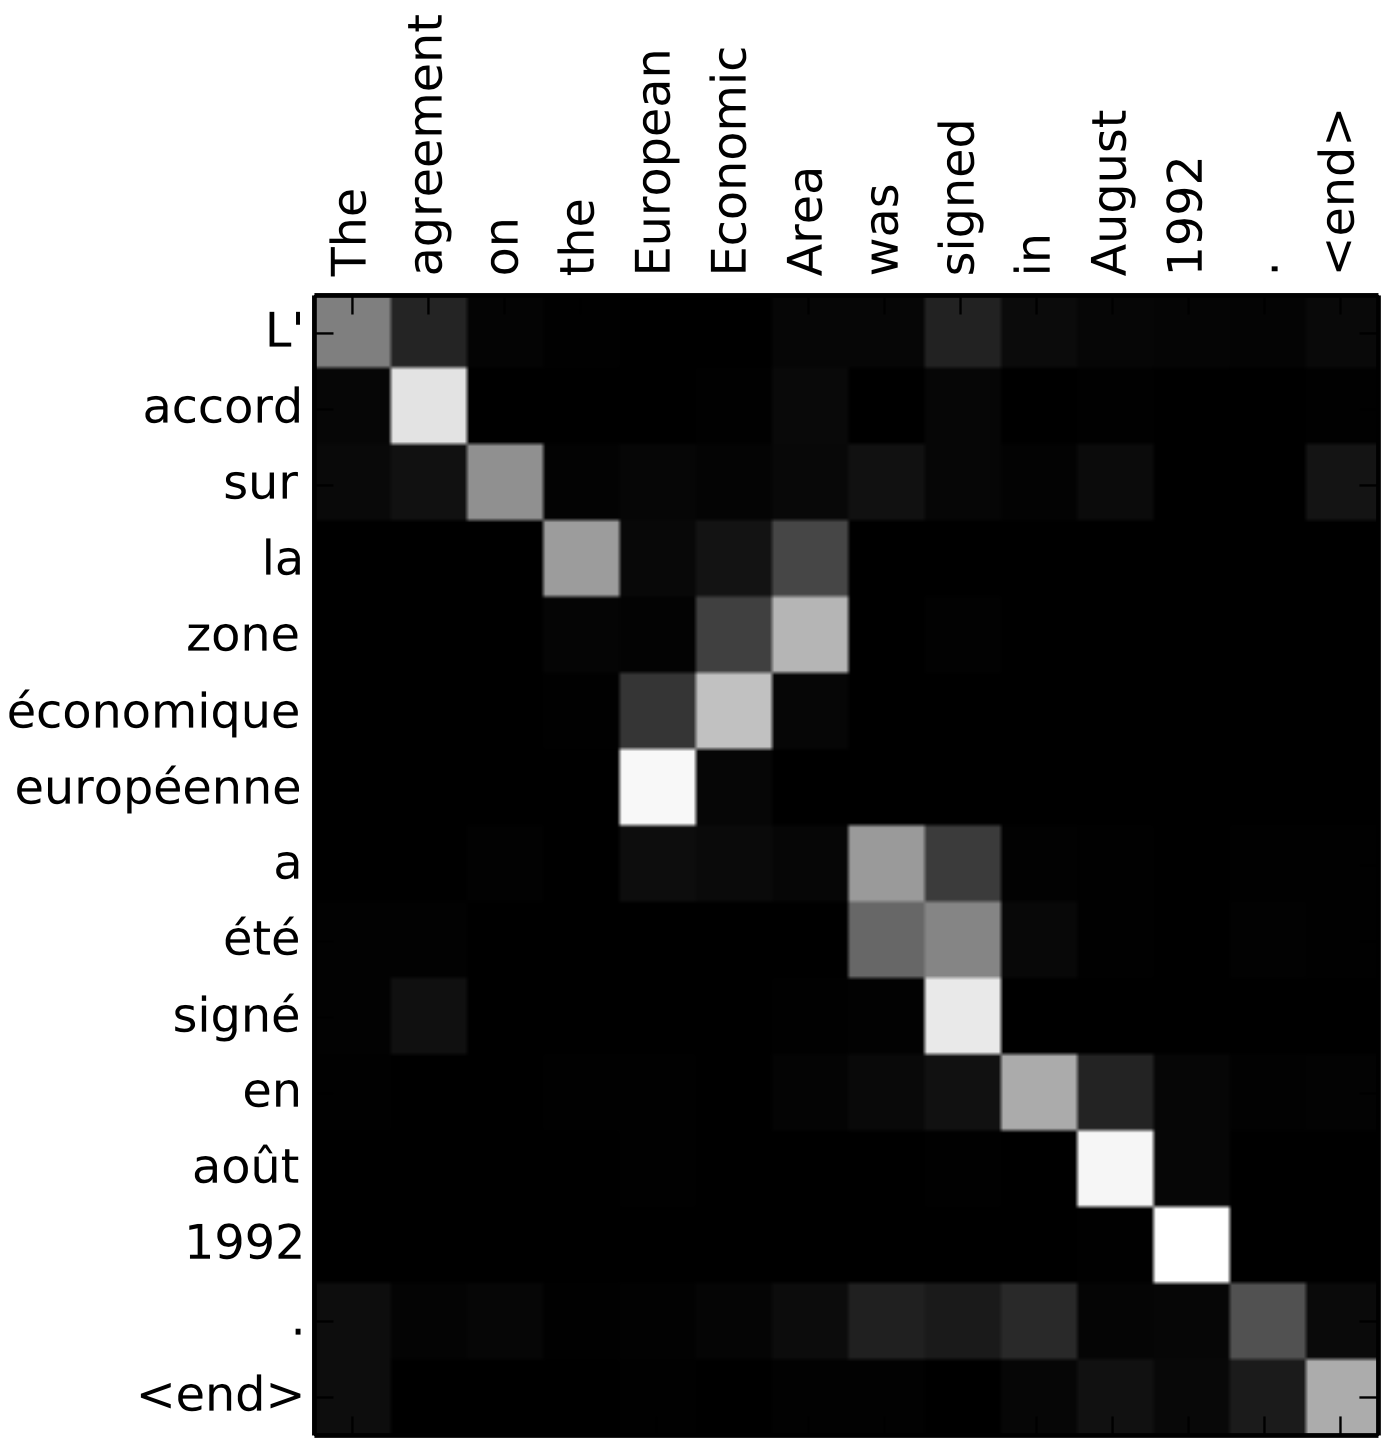
\includegraphics[scale=0.3]{2_production_mots_cles/attention_alignment.png}
    \caption{Exemple de visualisation des poids d'alignement du mécanisme d'attention entre une phrase en anglais et sa traduction en français. Chaque ligne montre la distribution des poids $\alpha_{t}$ ayant servis à générer le mot correspondant en français. Une case blanche indique un poids de 1, une case noire indique un poids de 0. Image extraite de \citet{bahdanau_neural_2014}.}
    \label{fig:attention_alignment}
\end{figure}

%Il faudra aussi porter attention à la syntaxe des deux langues
%Les poids d'attention peuvent être utilisés pour visualiser l'alignement entre les mots de la séquence d'entrée et ceux de la séquence de sortie.
%La figure~\ref{fig:attention_alignment} montre les poids d'alignement dans le cadre de la traduction automatique entre une phrase en anglais et sa traduction en français.

Le décodeur utilise l'état caché courant $h^d_t$ pour générer un mot, le mécanisme d'attention lui permet d'utiliser aussi tous les états cachés de l'encodeur $h^e$ pour mettre à jour l'état caché du décodeur $h^d_t$. Ce mécanisme est décrit dans l'équation~\ref{eq:attention}.
Dans le mécanisme d'attention, les états cachés $h^e$ sont pondérés en fonction de leur importance pour générer le mot $\hat{y}_t$.
Cette importance est établie grâce à une fonction d'alignement $a$ qui calcule une similarité entre l'état caché courant $h^d_t$ et ceux de l'encodeur $h^e$.
Les états cachés $h^e$ sont ainsi moyennés dans le vecteur de contexte $c_t$ utilisé pour mettre à jour l'état caché courant du décodeur $h^d_t$.

Dans l'équation \ref{eq:attention}: $[u;v]$ représente l'opération de concaténation des vecteurs $u$ et $v$; $a$ est une fonction d'alignement qui calcule la similarité entre un état caché de l'encodeur $h^e_t$ et du décodeur $h^d_t$; $\alpha$ représente les poids d'alignement entre les états cachés de l'encodeur $h^e$ et du décodeur $h^d$;  et $\textsc{Softmax}$ est une fonction qui normalise les valeurs d'un vecteur pour qu'il somme à 1.


\iffalse
    \begin{figure}
        \centering
        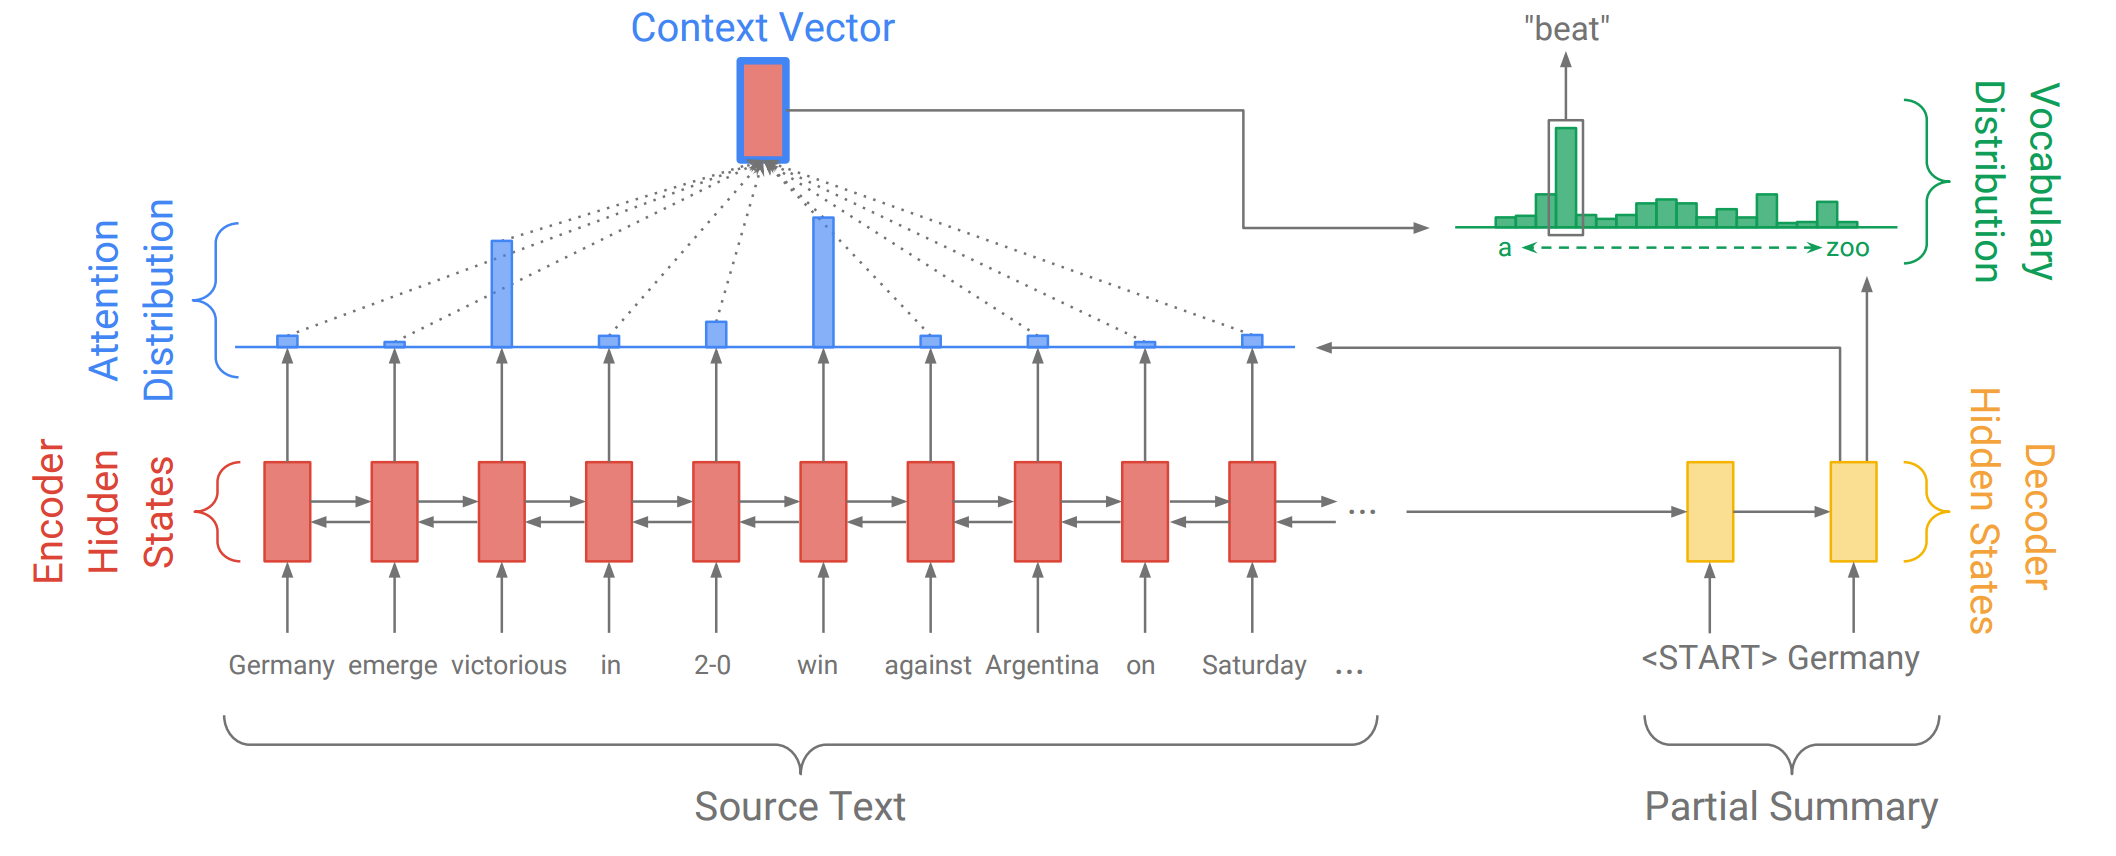
\includegraphics[width=\linewidth]{figures/see_seq2seq-attn.png}
        \caption{Schéma du mécanisme de copie présenté par \cite{see_get_2017}.}
        \label{fig:see_attention}
    \end{figure}
\fi

\begin{equation}\label{eq:attention}
  \begin{split}
    %\hat{Y}_t & = \sigma(b_v + W_v * h^d_t) \\
    p(y_t|y_{<t},x) & = \textsc{Softmax}(\sigma(W_v h^d_t)) \\[.3em]
    h^d_t & = \textsc{Rnn}(y_{t-1}, [h^d_{t-1};c_t]  \\[.3em]
    c_t & = \sum^{|h^e|}_{i=0} \alpha_{i,t} h^e_i \\
    \alpha_{t} & = \textsc{Softmax}(a(h^d_t, h^e)) \\
    %\textsc{Softmax}(x) & = \left[ \frac{x_i}{\sum^{|x|}_{i=0} x_i} , i \in |x| \right]
  \end{split}
\end{equation}

%Le concept d'attention a été présenté de deux manières différentes par \cite{bahdanau_neural_2014} et \cite{luong_effective_2015}.
%
%L'idée de l'attention présentée par~\cite{luong_effective_2015} est \emph{d'utiliser le vecteur de contexte pour prédire $y_t$}.
%
%\cite{bahdanau_neural_2014} présente un autre mécanisme d'attention dont l'idée est de calculer l'état caché du décodeur à l'aide d'un vecteur de contexte. Par rapport à un décodeur classique, seul le calcul de $h^d_t$ change.

\iffalse
    L'idée de l'attention présentée par~\cite{luong_effective_2015} est \emph{d'utiliser le vecteur de contexte pour prédire $y_t$}.
    
    Pour cela, un nouveau $\hat{h}^d_t$ est calculé en fonction d'un vecteur de contexte $c_t$ et de $h^d_t$ (calculé en fonction de $y_{t-1}$ et $h^d_{t-1}$). $c_t$ est la moyenne des $h^e$ pondérés par les scores d'alignement $\alpha$.
    
    Dans leur article, deux manières de calculer l'attention sont présentées: une attention globale et une attention locale.
    %
    Pour l'attention globale, le vecteur de contexte est la moyenne pondérée de toutes les représentations de l'encodeur.
    %
    Pour l'attention locale, le vecteur de contexte est la moyenne pondérée des représentations $h^e$ dans une fenêtre de taille $D$ autour de $h^e_{p_t}$.
    %
    $p_t$ est une valeur entre 0 et $|h^e|$ qui définit le centre de la fenêtre, et peut être calculé de différentes manières.\footnote{Pour plus de détails voir la section 3.2 de \cite{luong_effective_2015}}
    %$p_t$ étant $t$ (dans la traduction automatique on considère que le mot cible $y_t$ est aligné avec le mot source $x_{p_t}$), ou alors un réel entre 0 et $|h^e|$ calculé à l'aide 
    
    \begin{align}
        %y_t & = \sigma(W_v h^d_t) \\
        p(y_t | y_{<t}, x) & = \textsc{Softmax}(W_v \hat{h}^d_t) \\
        \hat{h}^d_t & = \sigma(W_c [c_t;h^d_t]) \\
        c_t & = \sum^{|h^e|}_{i=0} \alpha_{i,t} * h^e_i \\
        \alpha_{i,t} & = \textsc{Softmax}(a(h^e_i, h^d_t)) \\
        h^d_t & = \textsc{Rnn}(y_{t-1}, h^d_{t-1})
    \end{align}
    
    \cite{bahdanau_neural_2014} présente un autre mécanisme d'attention dont l'idée est de calculer l'état caché du décodeur à l'aide d'un vecteur de contexte. Par rapport à un décodeur classique, seul le calcul de $h^d_t$ change. Le calcul du vecteur de contexte est similaire à celui de ~\cite{luong_effective_2015}.
    
    \begin{align}
        p(y_t|y_{<t},x) & = \textsc{Softmax}(W_v h^d_t) \\
        h^d_t & = \textsc{Rnn}(y_{t-1}, [h^d_{t-1};c_t]  \\
        c_t & = \sum^{|h^e|}_{i=0} \alpha_{i,t} * h^e_i \\
        \alpha_{i,t} & = \textsc{Softmax}(a(h^e_i, h^d_t))
    \end{align}
    
    Il existe différentes fonctions d'alignement:
    
    bahdanau $a(h^e_i, h^d_t) = v_a \text{tanh}(W_a h^d_t + U_a h^e_i)$
    
    dot $a(h^e_i, h^d_t) = h^e_i h^d_t$
    
    general $a(h^e_i, h^d_t) = h^e_i W_a h^d_t$
    
    concat $a(h^e_i, h^d_t) = W_a [h^e_i;h^d_t]$
\fi

\subsubsection{Mécanisme de copie}
\label{sub:copy_mecanism}

Le mécanisme de copie~\cite{see_get_2017,gu_incorporating_2016} provient des tâches de traduction automatique et de résumé automatique. Il a pour but de produire des mots peu fréquents ou hors du vocabulaire de sortie.
En effet, les modèles neuronaux qui génèrent du texte choisissent les mots dans un vocabulaire de sortie comportant généralement \num{50 000} mots.
Dans les tâches sus-citées, les mots peu fréquents qui ne font pas partie du vocabulaire de sortie, comme les entités nommées ou les transfuges, doivent pourtant apparaître dans la séquence de sortie.
%Le mécanisme de copie ~\cite{see_get_2017,gu_incorporating_2016} pallie ce problème en permettant au décodeur de générer un mot du vocabulaire de sortie ou bien de copier un mot du document.
Deux mécanismes de copie ont été proposés par \citet{see_get_2017} et \citet{gu_incorporating_2016}; les deux étant similaires, nous présentons ici le premier car plus simple. Il est décrit dans l'équation~\ref{eq:copy_mecanism}.

% exemple
%Le mécanisme d'attention a été utilisé comme post-traitement pour remplacer les mots inconnus de la sortie par les mots de l'entrée alignés par le mécanisme d'attention. Ceci permettant de traiter les entités nommées peu fréquentes ou les transfuges.
%
%Le mécanisme de copie vient automatiser ce processus en permettant au modèle de générer un mot du vocabulaire ou de copier un mot du document.

%, tous deux inspirés des réseaux de pointeurs~\cite{vinyals_pointer_2015} qui génèrent une séquence de pointeurs vers la séquence d'entrée.
Ce mécanisme utilise le vocabulaire de la séquence d'entrée $\mathcal{X}$ (particulier à chaque document) en plus du vocabulaire de sortie $\mathcal{V}$.
Pour produire un mot, une distribution de probabilité sur le vocabulaire  $P_{vocab}(y_{t})$ est calculée comme précédemment par le décodeur (cf. section~\ref{sub:decoding}) et les poids du mécanisme d'attention $\alpha$ (cf. section~\ref{sub:attention_mecanism}) sont utilisés pour estimer la probabilité de copie de chaque mot du document.
Les poids d'attention $\alpha$ des mots qui apparaissent plusieurs fois dans l'entrée $x$ sont sommés $\sum_{j,x_j=y_{t,i}} \alpha^t_j$.
Ainsi, un mot peut être généré à partir du vocabulaire de sortie $\mathcal{V}$ ou copié à partir du vocabulaire du document $\mathcal{X}$.
Les probabilités de copie et de génération d'un même mot, qui appartient au document et au vocabulaire, sont sommées.
Dans l'équation~\ref{eq:copy_mecanism}: $h^d_t$, $c_t$ et $\alpha^t_j$ proviennent du mécanisme d'attention (cf. équation~\ref{eq:attention}); $p_{gen}$ est un curseur permettant au modèle de privilégier la copie ou la génération et $P_{vocab}(y_t)$ est une distribution de probabilité sur le vocabulaire de sortie $\mathcal{V}$.

%Les probabilités de génération et de copie sont combinés pour donner une distribution de probabilités sur $\mathcal{X} \cup \mathcal{V}$.

\begin{equation}\label{eq:copy_mecanism}
  \begin{split}
    p(y_{t,i}|y_{<t},x) & = p_{gen} P_{vocab}(y_{t,i}) + (1 - p_{gen}) \sum_{j,x_j=y_{t,i}} \alpha^t_j \\
    p_{gen} & = \sigma(W_h h^d_t + W_c c_t + W_y y_{t-1}) \\
    P_{vocab}(y_{t}) & = \textsc{Softmax}(\sigma(W_v h^d_t))
  \end{split}
\end{equation}

%ou les poids d'un mécanisme d'attention supplémentaire, utilisé seulement pour calculer le score de copie, pour~\cite{gu_incorporating_2016}

\iffalse
    %\cite{gu_incorporating_2016}, création d'un vocabulaire spécifique a chaque instance, composé de $\mathcal{V}$ le vocabulaire normal et $\mathcal{X}$ le vocabulaire des mots de l'entrée.
    %
    %Ça change le calcul de $y_t$ par rapport au mécanisme d'attention.
    %
    %On défini les vecteurs $\psi_g \in \mathds{R}^|\mathcal{V}|$ et $\psi_c \in \mathds{R}^|\mathcal{X}|$ qui contiennent respectivement les score de copie et de génération.
    
    % attentive read = les poids de l'attention
    % selective read = les poids de l'"attention" du mécanisme de copie
    
    \begin{align}
        y_t & = \textsc{Softmax}(e^{P_{gen}} +e^{P_{copy}}) \\
        P_{gen} & = W_v h^d_t \\
        P_{copy} & = \left[ \sum^{|h^e|}_{j=0, x_j=x_i} \sigma(h^e_j W_c) h^d_t | x_i \in \mathcal{X} \right] \\
        h^d_t & = RNN([y_{t-1};cc_t)],h^d_{t-1}) \\
        cc_t & = \sum^{|h^e|}_{i=1} aa_{t,i} h^e_t \\
        aa_{t,i} & = \textsc{Softmax}()
    \end{align}
    
    %\cite{see_get_2017} reprend le mécanisme d'attention de \cite{luong_effective_2015} et modifie le calcul de $y_t$ en ajoutant une probabilité de copie et un curseur privilégiant la copie ou la génération.
    
    \begin{align}
        p(y_{t,i}) = p_{gen} P_{vocab}(y_{t,i}) + (1 - p_{gen}) \sum_{j,x_j=y_{t,i}} \alpha^t_j \\
        p_{gen} = \sigma(W_c c_t + W_h h^d_t + W_y y_{t-1})
    \end{align}
\fi

% Multitache
% Conditional Random Field
% Reinforcement Learning : adaptative reward


\section{Méthodes de bout-en-bout}
\label{methodes-de-bout-en-bout}

\todo{Ajouter des schéma pour mieux comprendre les méthodes.}

Dans cette section nous présentons un état de l'art des méthodes de bout-en-bout.
Ces méthodes, contrairement aux méthodes en chaîne de traitement (cf. section~\ref{sec:methode-en-chaine-de-traitement}), prennent en entrée un document et laissent le soin au modèle d'en extraire les caractéristiques pour retourner un ensemble de mots-clés sans étapes intermédiaires ni définition manuelle de ces caractéristiques.
Parmi les méthodes proposées dans la littérature, nous distinguons les méthodes génératives, qui peuvent produire des mots-clés présents et des mots-clés absents, des méthodes extractives, limitées aux mots-clés présents.

Jusqu'à présent, toutes les méthodes de bout-en-bout qui ont été proposées sont supervisées et reposent sur des réseaux de neurones (cf. section~\ref{sub:neural_network}) qui nécessitent de grandes quantités de données annotées pour être entraînées.
%
Le développement de ces méthodes démarre avec l'introduction du jeu de données KP20k et de la méthode générative CopyRNN par \citet{meng_deep_2017}.
Le jeu de données KP20k, qui comporte $\simeq$\num{550000} documents, comble un manque.
En effet, seuls de petits jeux de données (de l'ordre du millier de documents) étaient jusqu'alors disponibles.
Ce travail a ainsi lancé une nouvelle direction de recherche sur les méthodes génératives de production de mot-clés.

\begin{figure}
    \centering
    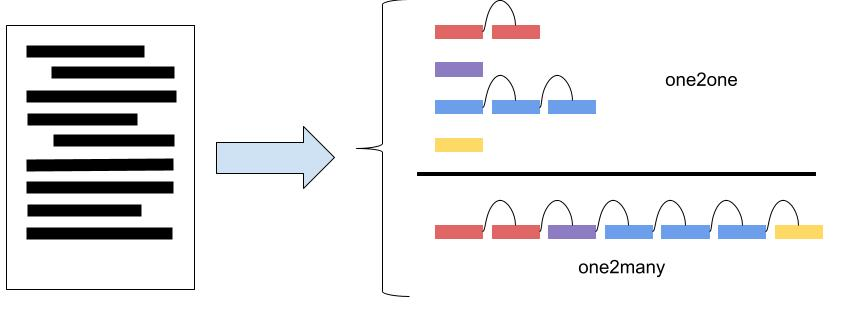
\includegraphics[scale=0.4]{2_production_mots_cles/Decoding strategies.jpg}
    \caption{Représentation schématique des stratégies de décodage \emph{one2one} et \emph{one2many}.}
    \label{fig:decoding_strategies}
\end{figure}
\todo{Refaire en tikz}

Dans cet état de l'art, nous présentons tout d'abord les méthodes automatiques de génération de mots-clés de bout-en-bout, qui sont au c\oe{}ur de ce travail de thèse.
Nous présentons ces méthodes de génération en deux parties: premièrement, les méthodes qui générent les mots-clés un à un (\emph{one2one}), et deuxièmement, celles qui génèrent des séquences de mots-clés (\emph{one2many}). Ces deux types de génération sont schématisés dans la figure~\ref{fig:decoding_strategies}.
Nous présentons ensuite les méthodes extractives de bout-en-bout, c'est-à-dire celles qui se limitent aux seuls mots-clés présents.

\subsection{Génération de mots-clés}
\label{sub:generation_de_mots_cles}

Les méthodes génératives, introduites par \citet{meng_deep_2017}, ont pour objectif de pallier deux faiblesses qui concernent la majorité des méthodes extractives présentées précédemment: l'impossibilité de produire des mots-clés absents ainsi que la faible prise en compte de la sémantique.
Le paradigme encodeur-décodeur sur lequel les méthodes génératives sont fondées permet d'encoder la sémantique du document.
Ainsi, les mots-clés produits sont le fruit d'une \say{compréhension} du document, contrairement aux méthodes en chaîne de traitement qui s'intéressent à l'\say{importance} des mots dans le document indépendamment de leur sens.
%
Ces méthodes génératives rendent possible la production de mots-clés absents grâce à la manière dont le décodeur génère la séquence de sortie.
Ce processus s'effectue en choisissant, à chaque étape de décodage, un mot à partir d'un vocabulaire de sortie qui est plus grand et différent du vocabulaire du document.
Ces méthodes génératives apprennent à générer des mots-clés un par un (génération \emph{one2one}, voir figure~\ref{fig:decoding_strategies}), c'est-à-dire que chaque document $X$ et son ensemble de mot-clés $Y$ de taille $N$ forment un couple $(X, \{Y_0, ..., Y_N\})$, décomposé en autant d'exemples d'entraînement que de mots-clés, $(X, Y_0), ... , (X, Y_N)$.

%\paragraph{Définitions}
%\todo{Il faudrait définir avant les principaux modèles: one2one, séquence avant de les définir formellement; Fait ausi des dessins}
%$x$ et $y$ représentent des mots, $p$ des mots-clés. Étant donné un ensemble de données $D = {(x^i,p^i), i \in 1...N}$ de taille $N$, un exemple est composé d'un document $x^i$ et d'un ensemble de mots-clés $p^i = {p^i_j, j \in 1...M^i}$ de taille $M^i$. Les documents et les mots-clés sont composés de mots $[x^i_k, k \in 1...N^i]$ et $[y^i_j]$ est composé d'un document composé d'une séquence de mots $x^i = (x^i_1, ..., x^i_{N^i})$ de longueur $N^i$ et d'un ensemble de mots-clés $p^i$ de taille $M^i$ avec $p^i = (p^i_1, ..., p^i_{M^i})$, où chaque mot-clé est une séquence de mots de taille $M^{i,j}$ avec $p^{i,j} = (y^{i,j}_1, ..., y^{i,j}_{M^{i,j}})$. Dans le cadre des modèles one2one, un couple document -- mots-clés est découpé en $M^i$ différents couples $(x^i, p^{i,1}), ..., (x^i, p^{i, M^i})$. 
%Pour les modèles en séquences, les mots-clés sont concaténés de sorte à former une unique séquence $(x^i, y^{i,1}_1 \lozenge ... \lozenge y^{i,1}_{M^{i,j}} \lozenge \text{SEP} \lozenge y^{i,2}_1 \lozenge ... \lozenge y^{i,M^i}_{M^{i,j}})$.

La méthode pionnière de génération automatique de mots-clés appliquée aux documents scientifiques est CopyRNN~\cite{meng_deep_2017}.
%
L'architecture neuronale de cette méthode s'inspire du processus d'annotation humain qui consiste à lire le document pour le comprendre dans son entièreté puis à le résumer grâce à des mots-clés.
%Aussi, les humains peuvent facilement s'abstraire du texte et faire appel à leurs connaissances pour produire des mots-clés qui n'apparaissent pas dans le texte.
Pour reproduire ce processus, CopyRNN utilise le paradigme encodeur-décodeur, que nous avons présenté dans la section~\ref{sub:paradigme_encodeur_decodeur}, pour encoder un document et le décoder ensuite en un mot-clé. % Ainsi un réseau de neurones récurrent encode le document dans un vecteur de pensée, puis un autre décode, génère, ce vecteur de pensée en un mot-clé.
Pour améliorer les performances des modèles encodeur-décodeur, il est commun d'utiliser un mécanisme d'attention (voir section~\ref{sub:attention_mecanism}).
Ce mécanisme permet au modèle de porter attention à certaines parties du document lors de la génération d'un mot.
%
Un mécanisme de copie est aussi ajouté au modèle pour lui permettre de générer des mots peu fréquents (voir section~\ref{sub:copy_mecanism}).
Ce mécanisme de copie modifie le décodage en permettant de générer un mot à partir du vocabulaire de sortie ou bien à partir du document.\\
%
Cette méthode obtient des performances bien plus élevées que les précédentes méthodes extractives. Les performances de CopyRNN sont de l'ordre de 30 points de \fmesure{} pour les mots-clés présents tandis que les performances des méthodes extractives sont généralement en dessous de 20 points de \fmesure{}.
Les mots-clés absents, qui ne pouvaient jusque-là pas être produits, correspondent peu à la référence: parmi les 50 meilleurs mots-clés absents un seul apparaît dans la référence.


%La communauté scientifique présente de nouvelles méthodes basées sur CopyRNN et tente de l'améliorer.
% les méthodes essaient de résoudre les problèmes identifiés
%Les méthodes présentées augmentent toujours les performances de génération des mots-clés présents et absents.

Certaines méthodes proposées essaient d'améliorer l'encodage du document.
\citet{chen_title-guided_2019}, par exemple, constate que les mots-clés ne sont pas uniformément distribués dans les documents.
En particulier \npercent{60} des mots-clés de référence ont au moins un mot en commun avec le titre du document.
Pour prendre cela en compte, ils proposent TGNet (Title Guided Network), qui étend CopyRNN en introduisant un nouvel encodeur spécifique au titre, en plus de l'encodeur du document.
Cet encodage du titre permet de donner un poids supplémentaire à l'information qu'il contient.
Ces deux représentations (du titre et du document) sont ensuite combinées puis fournies au décodeur.
Cette méthode améliore nettement les performances de génération des mots-clés présents et absents par rapport à CopyRNN (+\npercent{5} sur KP20k).
% Ils ne regardent que la F-mesure présent/absent rien d'autre

La redondance dans les ensembles de mots-clés produits est un problème récurrent dans les méthodes de production de mots-clés.
En effet, \citet{hasan_automatic_2014} montrent que 8 à \npercent{12} des erreurs des méthodes sont liées à la redondance des mots-clés.
Ainsi, les méthodes en chaîne de traitement mettent en place des stratégies, notamment lors de la sélection du sous-ensemble de mots-clés, pour limiter cette redondance (voir section~\ref{choisir-le-sous-ensemble}).
Dans cette ligne de recherche, \citet{zhao_incorporating_2019} remarquent les méthodes de bout-en-bout ne sont pas exemptes de ce problème, ils s'intéressent ainsi au chevauchement entre les mots-clés générés et ceux de référence.
Par exemple, \npercent{23.98} des mots-clés unigrammes générés par CopyRNN font partie d'un mot-clé de référence, et \npercent{47.15} des mots-clés 4-grammes générés par CopyRNN contiennent un mot-clé de référence.
Dans l'optique de limiter ces chevauchement, ils présentent le modèle ParaNet$_T$+CoAtt qui entraîne le modèle, à générer à la fois les mots-clés et leurs étiquettes morphosyntaxiques, ainsi la syntaxe des mots-clés générés sera similaire à celle des mots-clés de référence.
Pour cela ils ajoutent au modèle CopyRNN un encodeur, pour les étiquettes morphosyntaxiques des mots du document, ainsi qu'un décodeur, pour celles du mot-clé.\footnote{Les étiquettes morphosyntaxiques du document et des mots-clés proviennent de l'outils Stanford CoreNLP.}
Les informations des deux décodeurs sont ensuite combinées et utilisées pour générer les mots-clés et leurs étiquettes morphosyntaxiques.
%Grâce à cette méthode, les mots-clés générés chevauchent moins les mots-clés de référence; par exemple le pourcentage de mot-clés 4-grammes contenant un mot-clé de référence a baissé de \npercent{10}.

\begin{figure}
    \centering
    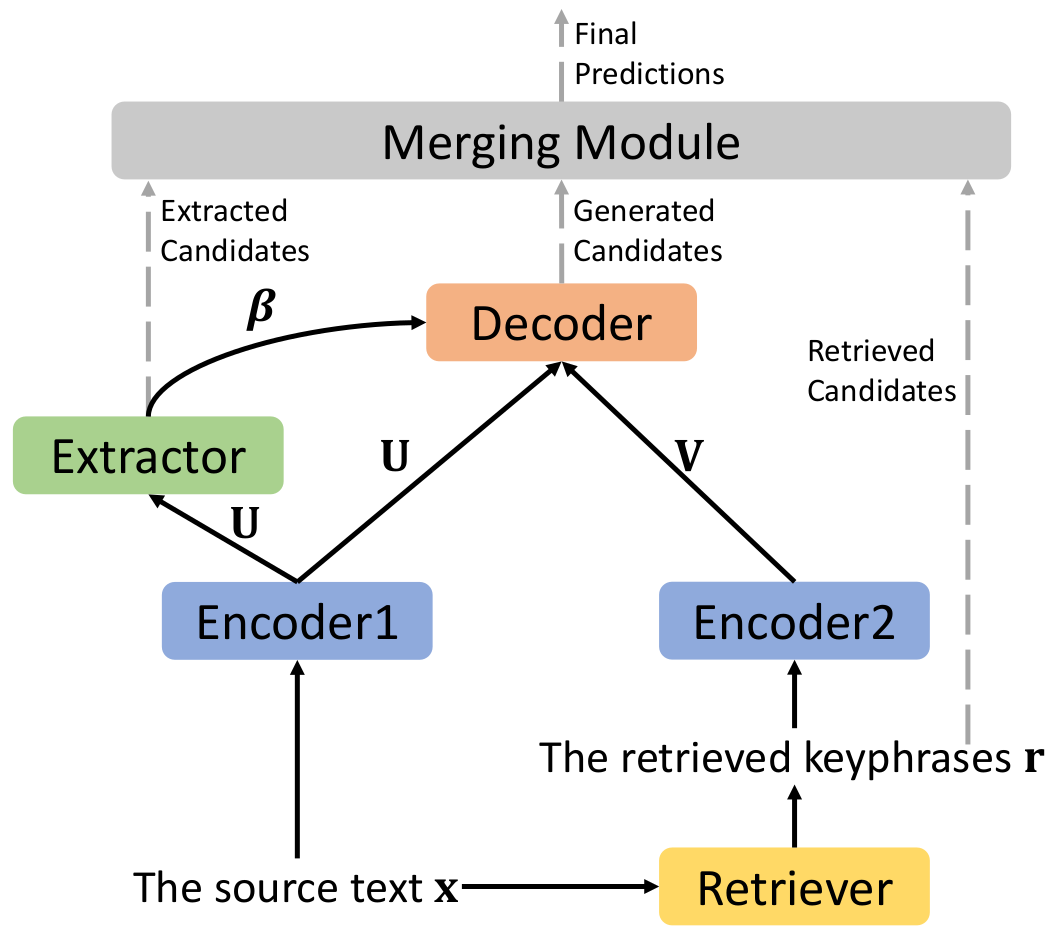
\includegraphics[scale=0.2]{2_production_mots_cles/kg_ke_kr_m.png}
    \caption{Représentation schématique de l'architecture de la méthode KG-KE-KR-M. Image extraite de~\citet{chen_integrated_2019}.}
    \label{fig:schema_kgkekrm}
\end{figure}

%Le processus manuel d'annotation en mots-clés est composé de plusieurs étapes: la lecture du document, l'extraction des mots-clés dans le document puis l'attribution de mots-clés absents du document et enfin la combinaison des mots-clés provenant de ces deux processus d'annotation.
Dans l'optique de reproduire l'annotation humaine, \citet{chen_integrated_2019} propose la méthode KG-KE-KR-M qui produit un ensemble de mots-clés en combinant différentes méthodes: génération de mots-clés, extraction de mots-clés, récupération de mots-clés (voir figure~\ref{fig:schema_kgkekrm}).
%Ces différentes méthodes sont entraînées de bout-en-bout puis les mots-clés de chaque méthode sont pondérés grâce à un classifieur.
%
Dans un premier temps, cette méthode récupère les mots-clés de référence des $K$ documents d'entraînement les plus proches du document traité (grâce à la distance de Jaccard).
Ces mots-clés \emph{récupérés} sont concaténés puis encodés. Ils serviront à conditionner la génération de mots-clés.
Dans un second temps, des mots-clés sont \emph{extraits} du document en classifiant chaque mot comme mot-clé ou non mot-clé.
%Cette classification s'effectue grâce aux états cachés du document encodé.
Ensuite, des mots-clés sont \emph{générés} à partir du document ainsi que des mots-clés récupérés et des mots-clés extraits.
Enfin, les mots-clés récupérés, extraits et générés sont pondérés grâce à un classifieur.
Cette méthode à la particularité de combiner les méthodes en chaîne de traitement (sélection de candidats puis pondération) et les méthodes de bout-en-bout (apprentissage conjoint de la génération et de l'extraction).
Malgré la grande diversité dans les techniques de production de mots-clés candidats, les performances ne sont pas significativement supérieures à CopyRNN. Cette méthode produit néanmoins plus de mots-clés absents de référence que CopyRNN.

La méthode CorrRNN~\cite{chen_keyphrase_2018} considère que les mots-clés doivent couvrir l'ensemble des sujets du document et être divers, c'est-à-dire que chaque mot-clé doit concerner un sujet différent.
Cette méthode étend CopyRNN en y ajoutant un mécanisme de couverture et un mécanisme de revue.
Le mécanisme de couverture encourage le modèle à porter attention aux différentes parties du document.
Il conserve et accumule les scores d'attention des mots du document à chaque étape de décodage, et il est inclus dans le calcul du mécanisme d'attention.
Ensuite, le mécanisme de revue est essentiellement un mécanisme d'attention sur les mots générés.
Son objectif est d'identifier les sujets déjà couverts par les mots-clés générés et ainsi de générer des mots-clés qui concernent des sujets non traités.
Cette méthode est la première à prendre en compte les mots-clés déjà générés dans le processus de génération, pour cela la phase d'entraînement est modifiée.
Au lieu de rétro-propager le gradient après chaque mot-clé de référence, la phase de rétro-propagation n'est effectuée qu'une fois tous les mots-clés de référence du document traités.
%Chaque mot-clé est généré en utilisant les mécanismes de couverture et de redondance, qui prennent en compte les mots-clés déjà générés; le gradient est ensuite calculé grâce à l'erreur de chaque mot-clé; et enfin, rétro-propagé.
%Cette méthode améliore les performance de production de mots-clés présent par rapport à CopyRNN, mais l'article ne présentant pas ses résultats sur le jeu de données de référence KP20k et utilisant des métriques peu utilisés dans les autres travaux la comparaison est limitée.

\subsection{Génération de séquences de mots-clés}% (\textsc{One2Seq})}
%\subsection{Génération en séquence}
\label{sub:generation_de_sequences_de_mots_cles}

%Nous avons présenté dans la section précédente, des méthodes génératives qui apprennent à générer un mot-clé par document.
Nous présentons dans cette section des méthodes qui apprennent à générer des séquences de mots-clés (génération \emph{one2many}, voir figure~\ref{fig:decoding_strategies}). C'est-à-dire que chaque exemple d'entraînement est composé d'un document et de la concaténation des mots-clés de référence en une unique séquence dans laquelle ils sont séparés par un symbole de séparation. Par exemple, l'ensemble de mots-clés $\{$ Classe , Fichier log , Agrégat $\}$ sera transformé en \say{Classe \texttt{SEP} Fichier log \texttt{SEP} Agrégat \texttt{FIN}}.
%Le développement des méthodes utilisant la génération \emph{one2many} part du constat que la génération \emph{one2one} ne permet pas de prendre en compte les mots-clés déjà générés et que les ensembles de mots-clés sont souvent redondants~\cite{hasan_automatic_2014}.
Le développement des méthodes génératives \emph{one2many} part du constat que les ensembles de mots-clés produits sont souvent redondants~\cite{hasan_automatic_2014} et que la génération \emph{one2one} ne permet pas de pallier ce problème.
En effet, les méthodes \emph{one2many} font l'hypothèse qu'avec la génération en séquence, le modèle ayant accès aux mots-clés déjà générés, il ne générera pas de mots-clés redondants.
%
Cette méthode de génération permet au modèle de générer le même nombre de mots-clés que la référence, en effet, il apprend en même temps qu'à générer les mots-clés, à placer les séparateurs de mots-clés et le symbole de fin.
Ainsi, ces méthodes peuvent générer des mots-clés selon deux stratégies~\cite{yuan_one_2020}: l'\textbf{inférence exhaustive} qui utilise l'algorithme de recherche en faisceau pour sur-générer des mots-clés et ainsi en obtenir un nombre fixe pour chaque document, c'est la stratégie employée par les méthodes génératives \emph{one2one}; et l'\textbf{inférence auto-régulée} (\foreign{self-terminating}) dans laquelle le décodage s'arrête lors de la génération du symbole de fin, cette stratégie permet au modèle de produire un nombre pertinent de mots-clés pour le document.
La seconde stratégie de décodage permet donc de s'affranchir du choix arbitraire du nombre de mots-clés $n$ à produire (voir section~\ref{choisir-le-sous-ensemble}).

Pour entraîner ces modèles, les mots-clés sont concaténés, mais ce processus n'est pas trivial.
En effet, l'ordre dans lequel les mots-clés sont concaténés influence les performances des modèles.
L'étude de \citet{meng_empirical_2021} compare différentes manières d'ordonner les mots-clés, telles que: \emph{No-Sort} qui laisse l'ordre par défaut; \emph{Alpha} qui trie par ordre alphabétique; \emph{Pres-Abs} qui place les mots-clés présents avant les mots-clés absents. L'étude montre que c'est l'ordre \emph{Pres-Abs} qui donne les meilleures performances.

La première méthode à générer des séquences de mots-clés est catSeqD~\cite{yuan_one_2020,yuan_generating_2018}.
L'objectif de cette méthode, similaire à CorrRNN, est d'augmenter la diversité des mots-clés générés.
%
Pour cela, le modèle CopyRNN, utilisé comme base, est augmenté d'un mécanisme de couverture sémantique et de régularisation orthogonale pour former le modèle catSeqD.
%
Le mécanisme de \emph{couverture sémantique} repose sur l'hypothèse que l'ensemble de mots-clés de référence et le document encodent la même information.
Ainsi, un nouvel encodeur est entraîné à encoder les mots-clés et à produire la même représentation que pour le document.
Il encode la séquence au fur et à mesure de sa génération et l'état cachés qui en résulte conditionne la prédiction du mot suivant, cela contraint les mots-clés générés à être proche sémantiquement du document.
%
Ensuite, les auteurs constatent que les mots générés après les séparateurs de mots-clés sont souvent similaires.
Le mécanisme de \emph{régularisation orthogonale} pallie ce problème en diversifiant explicitement les représentations des séparateurs, en pénalisant, dans la fonction de coût, ces représentations si elles ne sont pas orthogonales.

\todo{Refaire en Tikz}
\begin{figure}
    \centering
    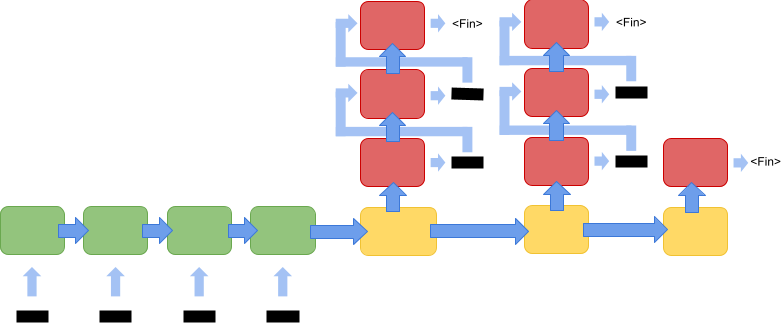
\includegraphics[scale=0.5]{2_production_mots_cles/exhird.png}
    \caption{Représentation schématique du décodage hiérarchique de la méthode ExHirD. L'encodeur du document est représenté en vert, le décodeur de concept en jaune et le décodeur de mots-clés en rouge.}
    \label{fig:schema_exhird}
\end{figure}

Dans le but de mieux modéliser les ensembles de mots-clés, \citet{chen_exclusive_2020} s'intéressent à la structure hiérarchique des ensembles de mots-clés.
En effet, les méthodes de génération de séquences de mots-clés identifient les mots-clés grâce à des marqueurs générés par le modèle. Cette séquentialité ne permet pas de représenter la hiérarchie entre les mots-clés et les mots qui les composent.
Ces travaux se rapprochent de \citet{yuan_generating_2018} qui essaient de rompre la séquentialité en modifiant la représentation des séparateurs de mots-clés avec le mécanisme de régularisation orthogonale.
Ainsi, ils présentent la méthode ExHirD~\cite{chen_exclusive_2020} dans laquelle le décodeur de l'architecture de CopyRNN est remplacé par un décodeur hiérarchique (voir figure~\ref{fig:schema_exhird}) qui génère les mots-clés en deux temps: d'abord l'identification des concepts, ensuite la génération de leur représentation textuelle.
Ce décodeur hiérarchique comprend un premier décodeur qui produit une représentation dense d'un concept, puis un second décodeur qui va générer une séquence de mots à partir de cette représentation dense pour instancier le concept en un mot-clé.
La génération des mots utilise deux mécanismes d'attention sur les documents d'entrée: l'un est conditionné par la représentation dense du concept; l'autre, standard, est conditionné par le mot précédent.
Ainsi, ce décodeur hiérarchique permet de modéliser explicitement les concepts importants du document et les mots qui les décrivent.
%
L'évaluation de cette méthode montre néanmoins un faible gain de performance, de l'ordre d'un point de F@5, pour les mots-clés présents et absents.
%
Ces travaux s'attellent aussi au problème de redondance des mots-clés et proposent un mécanisme de décodage exclusif pour tenter de le résoudre.
Ce mécanisme, simple dans son idée, interdit au modèle de générer deux mots-clés commençant par le même mot.
En effet, les mots-clés comportent le plus souvent entre 1 et 4 mots (voir section~\ref{sub:nature_linguistique}), ainsi le premier mot affecte grandement les suivants.
Ce mécanisme n'est pas limité à la méthode ExHirD; il peut être adapté aux différents types de décodage ou être utilisé en post-traitement.
Son évaluation montre qu'il fait significativement baisser le nombre de mots-clés dupliqués sans faire baisser les scores de F@5.

Les méthodes génératives \emph{one2many} apprennent à déterminer le nombre de mots-clés à produire mais en génèrent trop peu: catSeqD génère en moyenne 4,3 mots-clés par document alors que la référence en est composée de 5,3 en moyenne.
Les travaux de \citet{chan_neural_2019} s'intéressent à encourager les modèles à générer plus de mots-clés, en les entraînant à optimiser le rappel et la \fmesure{}.
Or ces métriques ne peuvent être utilisées comme fonction de coût dans l'algorithme de descente de gradient, car elles ne sont pas dérivables.
Pour résoudre ce problème, les auteurs proposent d'utiliser l'apprentissage par renforcement pour affiner\footnote{\foreign{To fine-tune} en anglais.} des modèles déjà entraînés.
%
Dans l'apprentissage par renforcement~\cite{williams_simple_1992}, un agent produit une série d'actions en suivant une politique (ici la génération de mots grâce à un modèle génératif), puis est récompensé pour chacune des actions.
%Dans l'apprentissage par renforcement~\cite{williams_simple_1992}, un agent produit une série d'actions en suivant une politique puis il est récompensé pour chaque action.
%Dans notre cas, une action consiste à générer un mot, la politique permettant de choisir le mot est un modèle génératif, et la récompense est le rappel ou la f-mesure.
L'algorithme d'apprentissage par renforcement optimise ainsi les poids du modèle (met à jour la politique) en fonction de la récompense.
%
Dans la méthode proposée, la récompense s'adapte selon le nombre de mots-clés générés: s'il est trop faible, la récompense sera le rappel pour encourager le modèle à générer plus de mots-clés; à l'inverse s'il est trop grand, la récompense sera la \fmesure{}, pour encourager le modèle à générer seulement de bons mots-clés.
%
De plus, les mots-clés présents et absents sont récompensés séparément pour favoriser la génération des mots-clés absents.

%CDKGen~\cite{diao_keyphrase_2020} (use close docs to encode, transformers)
%SenseNet~\cite{luo_sensenet_2020} (??)

Les travaux, concernant les méthodes neuronales, présentés jusqu'à présent considèrent que la quantité de données disponibles est suffisante.
Nous verrons dans le chapitre~\ref{chap:framework} que les sources de données contenant des documents annotés en mots-clés sont peu nombreuses malgré la large disponibilité de documents scientifiques en ligne.
Ainsi, les travaux de \citet{ye_semi-supervised_2018} se placent dans un cadre où la quantité de documents annotés est limitée.
%
Pour cela, les auteurs proposent deux méthodes qui tirent parti de la masse de documents non annotés pour la génération de mots-clés.
%
La première méthode consiste à utiliser des documents non annotés en mots-clés dans le cadre d'apprentissage multitâche.
Un réseau de neurones encodeur-décodeur est entraîné, pour les documents annotés, à générer des séquences de mots-clés et, pour les documents non annotés, à générer le titre du document. Dans le modèle, deux décodeurs différents sont utilisés pour chacune des tâches mais l'encodeur est partagé.
%
La seconde méthode consiste à créer un corpus synthétique en annotant automatiquement des documents en mots-clés. Les mots-clés sont extraits grâce aux méthodes \tfidf{} et TextRank.
Ainsi, un modèle de génération de mots-clés est pré-entraîné grâce à la combinaison des corpus synthétique et annoté, puis affiné grâce au seul corpus annoté.
%
L'évaluation des deux modèles résultant de ces méthodes d'entraînement montre qu'ils obtiennent des résultats similaires.
Les scores de F@5 pour les mots-clés présents des modèles semi-supervisés sont comparables à ceux du modèle \emph{catSeq} (CopyRNN entraîné à générer des séquences de mots-clés), bien qu'ils n'utilisent qu'un dixième des documents annotés utilisés par \emph{catSeq}.

\subsection{Extraction de mots-clés}

% Chapeau
Les méthodes génératives de bout-en-bout sont très performantes pour produire des mots-clés présents, mais génèrent très peu de mots-clés absents.
Ainsi, la communauté scientifique s'intéresse à des méthodes de bout-en-bout exclusivement extractives.
%Les méthodes génératives de bout-en-bout sont très performantes pour produire des mots-clés présents, ainsi la communauté scientifique s'intéresse à 
%Les méthodes génératives de bout-en-bout, qui ont la particularité de produire des mots-clés absents, n'en produisent au final que très peu~\cite[inter alia]{chen_exclusive_2020, santosh_hicova_2021} et ceux-ci ne correspondent que très peu aux mots-clés de référence~\cite[inter alia]{ahmad_select_2020, ye_one2set_2021}.
%Mais leurs performances élevées pour produire des mots-clés présents encouragent tout de même le développement de méthodes de bout-en-bout.
%C'est pourquoi la communauté scientifique s'intéresse aux méthodes de bout-en-bout exclusivement extractives.
%
Bien qu'elles ne soient pas au c\oe{}ur de nos travaux, nous présentons les principales méthodes extractives par soucis d'exhaustivité.
% Plan
Dans cette section nous présentons tout d'abord les méthodes fondées sur l'annotation en séquence, ensuite, une méthode de classification, et enfin, une méthode fondée sur les graphes.

Le développement de ces méthodes est lié à celui des modèles de langues pré-entraînés tels que BERT~\cite{devlin_bert_2019}, SciBERT~\cite{beltagy_scibert_2019} ou encore GPT-2~\cite{radford_language_2019} qui reposent sur l'architecture transformer~\cite{vaswani_attention_2017}.
Ils sont utilisés pour fournir des plongements de mots contextuels ou bien pour être affinés pour une tâche particulière.
Ces modèles, entraînés sur de très grandes quantités de données, ont permis d'améliorer significativement les performances de nombreuses tâches de traitement automatique de la langue~\cite{wang_glue_2018}.

% Annotation en séquence
\paragraph{Annotation en séquence}
La grande majorité des méthodes extractives de bout-en-bout reformulent la tâche de production de mots-clés en une tâche d'annotation en séquence.
Dans l'annotation en séquence, chaque mot du document est associé à une étiquette selon un schéma binaire: mot-clé ou non mot-clé, ou bien selon le schéma \texttt{BIO} dans lequel les mots du document correspondent au début (\texttt{B}), à l'intérieur (\texttt{I}) ou à l'extérieur (\texttt{O}) d'un mot-clé.\\
%
La méthode pionnière, proposée par \citet{augenstein_multi-task_2017}, utilise un encodeur récurrent bi-directionnel pour représenter chacun des mots et prédire leurs étiquettes.
Elle est amélioré par \citet{alzaidy_bi-lstm-crf_2019} qui ajoute un champ aléatoire conditionnel (CRF) pour améliorer la prédiction séquentielle des étiquettes, ainsi que par \citet{sahrawat_keyphrase_2019} qui utilise les plongements contextuels de BERT en entrée de l'encodeur.
%
La méthode SaSaKe~\cite{santosh_sasake_2020}, quant à elle, utilise les relations de dépendances syntaxique et sémantique du document pour améliorer la représentation des mots.
Le document est encodé puis les relations de dépendances sont représentées sous formes de graphes et incorporées aux représentations des mots grâce à des réseaux à convolution de graphes.
Ces représentation servent ensuite à étiqueter chaque mot comme mot-clé ou non mot-clé.
%La méthode pionnière, proposée par \citet{augenstein_multi-task_2017}, utilise un encodeur récurrent bi-directionnel pour représenter chacun des mots et prédire leurs étiquettes. D'autres travaux améliorent cette méthode, notamment BiLSTM-CRF~\cite{alzaidy_bi-lstm-crf_2019} qui ajoute à l'encodeur un champ aléatoire conditionnel (CRF), ce qui améliore la prédiction séquentielle des étiquettes. Dans la même ligne de recherche, \citet{sahrawat_keyphrase_2019} améliore BiLSTM-CRF en utilisant les plongements de mots contextuels de BERT en entrée de l'encodeur.\\
%
%D'autres méthodes pour l'annotation en séquence sont présentées, la méthode SaSaKe~\cite{santosh_sasake_2020} par exemple, prend explicitement en compte la syntaxe et la sémantique des documents grâce à leurs graphes de dépendances syntaxique et sémantique. Cette méthode encode le document grâce à un transformer puis incorpore à la représentation de chaque mot les informations des graphes de dépendances à l'aide de réseaux à convolution de graphe.\\
%
%De son côté, \citet{martinc_tnt-kid_2020} propose la méthode TNT-KID qui tire parti du transfert de connaissances d'un modèle de langue pré-entraîné et se place dans un contexte de données limitées. Cette méthode consiste d'abord à pré-entraîner un modèle de langue transformer à l'aide de données non annotées. Puis à affiner ce modèle grâce au seul ensemble de validation de KP20k pour l'identification de mots-clés grâce à l'annotation en séquence. Ainsi, avec seulement \num{20000} documents annotés cette méthode obtient des résultats comparables à ceux de CopyRNN.

% Classification
\paragraph{Classification}
La méthode BERT-JointKPE~\cite{sun_joint_2020} s'inspire des méthodes en chaîne de traitement pour entraîner un modèle de bout-en-bout à classifier chaque n-gramme du document comme mot-clé ou non mot-clé. Cette méthode ressemble donc à une sélection de mots-clés candidats n-grammes (voir section~\ref{selection-des-mots-cles-candidats}).
Les plongements des mots du document sont d'abord calculés à l'aide de BERT. Ensuite, grâce à des convolutions de différentes tailles, les représentations des mots sont agrégées pour représenter les n-gramme (de 1 à 5).
Enfin, chaque n-gramme est classifié comme mot-clé ou non mot-clé grâce à sa représentation dense.

% Enfin
\paragraph{Graphe}
La méthode DivGraphPointer~\cite{sun_divgraphpointer_2019} diffère des autres méthodes extractives car elle est fondée sur le paradigme encodeur-décodeur.
Nous la décrivons en détail pour comparer son architecture à celles des méthodes génératives décrites dans les sections~\ref{sub:generation_de_mots_cles} et \ref{sub:generation_de_sequences_de_mots_cles}.
%
Cette méthode combine la représentation sous forme de graphe, largement utilisée par les méthodes en chaîne de traitement (voir section~\ref{graphe}), et la génération de mots-clés en séquence (\emph{one2many}).%
\footnote{Cette méthode est générative, mais ne peut produire de mots-clés absents. En dehors de sa description nous réservons le terme \say{méthodes génératives} aux seules méthodes pouvant produire des mots-clés absents.}
L'intérêt de cette représentation est double: elle permet premièrement de mutualiser l'information des multiples occurrences d'un même mot; et deuxièmement, elle permet de prendre en compte les interactions entre les mots de manière globale.
%
Ainsi, le document est d'abord représenté sous forme de graphe dans lequel les n\oe{}uds représentent les mots et les arêtes la distance entre les positions des mots.
Ensuite, des couches de convolution de graphe calculent la représentation de chaque n\oe{}ud en fonction de ses voisins.
Ces représentations sont agrégées pour initialiser le décodeur, un \foreign{pointer network}~\cite{vinyals_order_2016}.
Enfin, ce décodeur produit une séquence de mot exclusivement copiée du document.
%
DivGraphPointer à pour objectif, comme \emph{catSeqD}, de produire des mots-clés peu redondants.
Ainsi, en plus du mécanisme d'attention et de couverture, le mécanisme de \emph{modification du contexte} (similaire dans son objectif à la \emph{régularisation orthogonale} de \emph{catSeqD}) recalcule l'état caché après avoir généré un séparateur de mot-clé.
Cet état caché est calculé en fonction de la représentation du document et de l'ensemble des mots-clés précédemment générés.\\
%
Un intérêt peu discuté de cette méthode est sa capacité à produire des mots-clés qui ne sont pas des sous-séquences du document mais dont tous les mots y apparaissent.
Ainsi, la dichotomie entre mots-clés présents et mots-clés absents ne semble ne pas convenir à ce type de mots-clés.
Nous discuterons la définition de mots-clés présents et de mots-clés absents dans le chapitre~\ref{chap:ri}.


\section{Conclusion}

% Méthodes en ch de traitement
%Nous avons vu dans le chapitre~\ref{chap:concepts} les méthodes de production automatique de mots-clés en chaîne de traitement.
%La communauté scientifique à proposé de nombreuses méthodes en chaîne de traitement qui utilisent différents descripteurs pour identifier les mots-clés les plus importants des documents.
%Ces méthodes nécessitent peu de données d'entraînement ou sont non supervisées.
%Elles ne dépendent généralement pas de la langue et peuvent être transposées simplement.
%
%Malheureusement, l'enchaînement des différentes étapes propage et intensifie les erreurs.
%De plus, la définition manuelle des descripteurs, qui nécessite des connaissances expertes, limite la transférabilité des méthodes à d'autres types de document.
%Enfin, ces méthodes en chaîne de traitement, majoritairement extractives, ne peuvent produire que des mots-clés qui sont présents dans le document.
%
%Pour pallier la propagation d'erreurs et la définition manuelle des descripteurs, des méthodes d'apprentissage profond de bout-en-bout sont proposées.
%Malgré leurs avantages, ces méthodes nécessitent d'être entraînées à l'aide de grandes quantités de données annotées.
%
%Ces méthodes sont cependant moins généralisables à d'autres genres de documents de par leur nature supervisée, ainsi qu'à d'autres langues car elles nécessitent des données annotées.
%
%De plus, leur complexité, leur variabilité dans leurs implémentations, leur temps d'exécution et d'entraînement sont aussi des limites à leur utilisation à grande échelle.
%paramètres à prendre en compte en fonction de l'utilisation qui en sera faite.

Dans ce chapitre, nous avons présenté les principes fondamentaux des réseaux de neurones ainsi que le paradigme encodeur-décodeur qui permet d'encoder un document de longueur variable et de générer une séquence de mots.
Nous avons ensuite présenté un état de l'art des méthodes de production de mots-clés de bout-en-bout, toutes neuronales, qui reposent à minima sur les encodeurs ou les décodeurs.
Pour cet état de l'art, nous avons séparé ces méthodes en deux catégories~: les méthodes génératives et les méthodes extractives.


% 2.1 fondements
% 2.1.1 neural nets
% 2.1.2 encodage
% 2.1.3 décodage
% 2.1.4 stratégies de décodages
% 2.1.5 encodeur-décodeur

La mise à disposition, par \citet{meng_deep_2017}, d'une grande quantité de données annotées permet le développement de méthodes de bout-en-bout pour la production de mots-clés.
Ces méthodes de bout-en-bout pallient certains écueils des méthodes en chaîne de traitement, présentées au chapitre~\ref{chap:concepts}, notamment la propagation des erreurs entre les différentes étapes et la définition manuelle des traits pour identifier l'importance des mots-clés.
%
Néanmoins, les méthodes de bout-en-bout ne sont pas exemptes de limites~: elles nécessitent de grandes quantités de données pour être entraînées ainsi qu'une grande puissance de calcul pour être utilisées.
%Elles introduisent néanmoins de nouvelles limitations: premièrement, la nécessité de disposer de grandes quantités de données annotées pour leur entraînement et deuxièmement, la disposition d'une grande puissance de calcul nécessaire à leur exécution.

Les méthodes extractives de bout-en-bout s'inspirent, pour la majorité, de l'annotation en séquence et entraînent des réseaux de neurones à identifier le début et la fin des mots-clés dans les documents.
Ces méthodes sont, de manière générale, plus performantes que les méthodes génératives, ainsi, la spécialisation des méthodes dans l'extraction de mots-clés semble faciliter la tâche.

%Les méthodes génératives, qui constituent le c\oe{}ur de nos travaux, entraînent un réseau de neurones à générer les mots-clés de référence.
%Ces méthodes ont la capacité de produire des mots-clés absents, ce que les méthodes proposées jusqu'alors ne permettaient pas.
%Cependant, l'analyse des mots-clés générés par ces méthodes montre que les mots-clés qui correspondent à la référence sont presque exclusivement des mots-clés présents.
%Ainsi, elles ne produisent en fait que très peu de mots-clés absents et ceux-ci ne correspondent que très peu à la référence.
%Nous verrons dans le chapitre~\ref{chap:ri} que ces mots-clés absents sont un enjeu important pour la tâche de recherche d'information.

Les méthodes génératives, qui constituent le c\oe{}ur de nos travaux, entraînent un réseau de neurones à générer les mots-clés de référence.
Elles ont la capacité de produire des mots-clés absents, ce que les méthodes proposées jusqu'alors ne permettaient pas.
Ces méthodes ont deux principales faiblesses: elles produisent très peu de mots-clés absents (1,7 en moyenne~\cite{chan_neural_2019}) et produisent des mots-clés très redondants (entre  \npercent{20} et \npercent{30}~\cite{chen_exclusive_2020}).
%
Ainsi, les différentes méthodes présentées ont pour objectif de pallier au moins une de ces faiblesses en ajoutant des mécanismes de diversification des mots-clés, en essayant d'améliorer la modélisation des documents ou en modifiant le processus de décodage.
De manière globale, les performances de la tâche de production automatique de mots-clés augmentent peu.
Notons tout de même l'amélioration des performances pour les mots-clés \emph{présents} de 33 à 40 points de F@5 sur KP20k entre les premiers travaux de \citet{meng_deep_2017} et ceux, plus récents, de \citet{ye_heterogeneous_2021}.
%La production de mots-clés présents augmente tout de même: les premiers travaux de \citet{meng_deep_2017} et ceux, plus récents, de \citet{ye_heterogeneous_2021} rapportent respectivement une F@5 sur KP20k de 33 et de 40 points.
%Mais la production de mots-clés absents, elle, stagne: \citet{chan_neural_2019} et \cite{ye_heterogeneous_2021} rapportent respectivement une F@5 sur KP20k de 1,5 et 3.
Mais, malgré cette augmentation de performance pour les mots-clés présents, les performances pour les mots-clés \emph{absents} ne dépassent pas 5 points de F@5~\cite{chan_neural_2019,ye_heterogeneous_2021}.
%
Nous verrons dans le chapitre~\ref{chap:ri} que ces mots-clés absents sont un enjeu important pour la tâche de recherche d'information.


%Premièrement, elles produisent très peu de mots-clés absents (1,7 en moyenne contre 3,9 pour les mots-clés présents ~\cite{chan_neural_2019}) et ceux-ci ne correspondent que très peu à la référence (avec une F@5 maximale de 3,6 atteinte par \citet{ye_one2set_2021}).
%Deuxièmement, les mots-clés générés sont très redondants, ceux-ci prennent la place de bon mots-clés possible \citet{chen_exclusive_2020} estime qu'entre \npercent{20} et \npercent{30} des mots-clés produits sont redondants.


%Les principaux problèmes des méthodes générative sont que les mots-clés produits sont très redondants, et que très peu de mots-clés absents sont effectivement généré (qu'ils correspondent à la référence ou pas).
%Ainsi les différentes méthodes présentées ont pour objectif de pallier l'un de ces problèmes en ajoutant des mécanisme ou en modifiant le processus d'entraînement des modèles.
%Les améliorations en terme de \fmesure{} de chaque méthode sont peu significatives.
%
%Les méthodes d'annotation en séquence, quant à elles, sont de manière générales plus performantes que les méthodes génératives.
%Ainsi, la spécialisation des méthodes dans l'extraction de mots-clés semble faciliter la tâche.
%Elles obtiennent, sur KP20k, des scores de l'ordre de 45 points de \fmesure{} pour les mots-clés présents, ce qui est supérieur aux méthodes génératives qui, pour l'instant, obtiennent des scores toujours inférieurs à 40 points de \fmesure{}.

\cleardoublepage
\chapter{Production de mots-clés de bout-en-bout} \label{chap:kw_production}

Ce chapitre présente les méthodes de production de mots-clés de l'état de l'art de bout-en-bout, qui constituent l'élément principal de ce travail de thèse. 
Nous commencerons par présenter les composants de ces méthodes auxquels nous feront référence dans la partie état de l'art.

\section{Principes fondamentaux des réseaux de neurones}
% Fondements sur les réseaux de neurones

Nous présentons dans cette section les concepts nécessaires à la bonne compréhension des méthodes de production de mots-clés de bout-en-bout.
Nous décrivons d'abord en détail les réseaux de neurones, ensuite les plongements de mots (\foreign{word embeddings}) utilisés pour représenter les mots du langage naturel, et enfin le paradigme encodeur-décodeur qui permet de traiter du texte de longueur variable en entrée et en sortie des réseaux de neurones.

Contrairement aux méthodes en chaîne de traitement décrites dans la section~\ref{sec:methode-en-chaine-de-traitement}, les méthodes de bout-en-bout, qui utilisent le paradigme encodeur-décodeur, se passent de l'identification des candidats ainsi que du choix des caractéristiques des mots-clés qui serviront à les pondérer.
En effet, les méthodes que nous décrivons dans ce chapitre utilisent des réseaux de neurones profonds qui apprennent à extraire automatiquement les descripteurs  les plus pertinents.
%L'apprentissage profond, permet de laisser le modèle extraire les descripteurs de manière automatique au lieu de les définir à la main, ce qui nécessite des connaissances expertes. Mais cela est difficile à interpreter, tout un pan de la recherche s'intéresse à expliquer ces méthodes (blackbox nlp)~\cite{}.


\subsection{Réseaux de neurones}
\label{sub:neural_network}

\begin{figure}
    \centering
    %Heavily inspired from https://texample.net/tikz/examples/neural-network/

\begin{tikzpicture}[shorten >=1pt,->,draw=black!50]
    \def\myscale{1.5}
    \tikzstyle{neuron}=[circle,fill=black!25,minimum size=17*\myscale,inner sep=0cm]
    \tikzstyle{input neuron}=[neuron, fill=color1!60];
    \tikzstyle{hidden neuron}=[neuron, fill=color0!60];
    \tikzstyle{output neuron}=[neuron, fill=color2!60];
    \tikzstyle{edge label}=[above=-.025cm,sloped,scale=.4*\myscale,black!60]
    \tikzstyle{label}=[scale=.75*\myscale, text width=2cm, align=center]

    \def\layersep{2.5*\myscale}
    \def\ninput{2}
    \def\nlayerone{3}
    \def\nlayertwo{2}
    \def\noutput{2}

    % Draw the input layer nodes
    \foreach \name / \y in {1,...,\ninput}
    % This is the same as writing \foreach \name / \y in {1/1,2/2,3/3,4/4}
        \node[input neuron] (I-\name) at (0,-\y*\myscale) {};


    % Draw the hidden layer nodes
    \foreach \name / \y in {1,...,\nlayerone}
        \path[yshift=.5*\myscale cm]
            node[hidden neuron] (H1-\name) at (1*\layersep,-\y*\myscale) {};

    \foreach \name / \y in {1,...,\nlayertwo}
        \path[yshift=.0*\myscale cm]
            node[hidden neuron] (H2-\name) at (2*\layersep,-\y*\myscale) {};

    % Draw the output layer node
    \foreach \name / \y in {1,...,\noutput}
        \path[yshift=0*\myscale cm]
            node [output neuron] (O-\name) at (3*\layersep,-\y*\myscale) {};

    % Connect every node in the input layer with every node in the
    % hidden layer.
    
    %\foreach \source in {1,...,\ninput}
    %    \foreach \dest in {1,...,\nlayerone}
    %        \draw[->] (I-\source) -- node [edge label, pos={.28-}] {$W^1_{\source,\dest}$} (H1-\dest);
    
    \def\layerout{1}
    \def\source{1}
    \foreach \dest / \n in {1/.2,2/.25,3/.235}
        \draw[->] (I-\source) -- node [edge label, pos={\n}] {$W^\layerout_{\source,\dest}$} (H\layerout-\dest);
    \def\source{2}
    \foreach \dest / \n in {1/.17,2/.285,3/.26}
        \draw[->] (I-\source) -- node [edge label, pos={\n}] {$W^\layerout_{\source,\dest}$} (H\layerout-\dest);


    \def\layerout{2} % modify this
    \pgfmathtruncatemacro{\layerin}{\layerout - 1}
    \def\source{1} % modify this
    \foreach \dest / \n in {1/.2,2/.26} % modify this
        \draw[->] (H\layerin-\source) -- node [edge label, pos={\n}] {$W^\layerout_{\source,\dest}$} (H\layerout-\dest);
    \def\source{2} % modify this
    \foreach \dest / \n in {1/.2,2/.25} % modify this
        \draw[->] (H\layerin-\source) -- node [edge label, pos={\n}] {$W^\layerout_{\source,\dest}$} (H\layerout-\dest);
    \def\source{3} % modify this
    \foreach \dest / \n in {1/.23,2/.3} % modify this
        \draw[->] (H\layerin-\source) -- node [edge label, pos={\n}] {$W^\layerout_{\source,\dest}$} (H\layerout-\dest);

    % Connect every node in the hidden layer with the output layer
    \def\layerout{3} % modify this
    \pgfmathtruncatemacro{\layerin}{\layerout - 1}
    \foreach \source in {1,...,\nlayertwo}
        \foreach \dest in {1,...,\noutput}
            \draw[->] (H\layerin-\source) -- node [edge label, pos={.20+(1-Mod(\dest,2))*.05}] {$W^\layerout_{\source,\dest}$} (O-\dest);

    % Annotate the layers
    \node[label, below=.1cm of I-\ninput] (I-label) {Entrée};

    \node[draw, dashed, rounded corners,fill=none, fit=(H1-1) (H1-\nlayerone)] (H1) {};
    \node[label, below=.1cm of H1] (H1-label) {Première couche};

    \node[draw, dashed, rounded corners,fill=none, fit=(H2-1) (H2-\nlayertwo)] (H2) {};
    \node[label, below=.1cm of H2] (H2-label) {Seconde couche};

    \node[draw, dashed, rounded corners,fill=none, fit=(O-1) (O-\noutput)] (O) {};
    \node[label, below=.1cm of O] (O-label) {Couche de sortie};

    \node[draw, dashed, rounded corners,fill=none, fit=(H1) (H1-label) (H2) (H2-label)] (H) {};
    \node[label, text width=10cm, below=.1cm of H] (H-label) {Couches cachées};

\end{tikzpicture}
    \caption{Représentation graphique d'un réseau de neurones à 2 couches. Les flèches représentent les poids des matrices $W^k$. Les biais $b^k$ ne sont pas représentés.}
    \label{fig:ex_nn_simple}
\end{figure}
% https://texample.net/tikz/examples/neural-network/

Les réseaux de neurones servent à modéliser des fonctions complexes, qui peuvent être non linéaires.
%
D'un point de vue mathématique, il s'agit de modéliser une fonction $f$ qui prend une entrée $X$ et retourne une sortie (une prédiction) $\hat{Y} = f(X)$.
%
Ici, $X \in M_{1,m}(\mathds{R})$ et $\hat{Y} \in M_{1,n}(\mathds{R})$ sont des vecteurs de taille $m$ et $n$ respectivement.
%
Ces vecteurs représentent le nombre de paramètres d'entrée de la fonction $f$.
%
%Par exemple, un modèle qui prédit le prix d'une maison en fonction de sa surface et du nombre de fenêtres aura 2 entrées et une sortie.


Un réseau de neurones simple (également appelé perceptron mono-couche) est défini par l'équation~\ref{eq:simple_nn} ci-dessous, dans laquelle $W$ est une matrice de poids $W \in M_{m, n}(\mathds{R})$ et $b$ un vecteur de biais $b \in M_{1,m}(\mathds{R})$.
%
\begin{align}
    \hat{Y} = f(X) = \sigma (b + W * X) \label{eq:simple_nn}
\end{align}


La fonction $\sigma$ est une fonction dite d'activation.
Elle est inspirée de l'activation des neurones dans le cerveau humain.
L'information d'un neurone passe à la couche suivante si le neurone est activé (c'est-à-dire si sa valeur est assez élevée).
Les fonctions Sigmoïde (voir équation~\ref{eq:sigmoide}) et Rectified Linear Unit (ReLU) (voir équation~\ref{eq:relu}) sont généralement utilisées pour $\sigma$.
%Cette fonction est généralement la fonction sigmoïde (équation~\ref{eq:sigmoide}), Rectified Linear Unit (ReLU) (équation~\ref{eq:relu}), ou tangente hyperbolique ($\text{tanh}$). \todo{comment choisir cette fonction ?}

\begin{gather}
    \sigma(x) = \frac{1}{1+e^{-x}} \label{eq:sigmoide} \\
    \textsc{ReLu}(x) = \text{max}(0, x) \label{eq:relu}
\end{gather}

%\begin{figure}\centering
%    \begin{tikzpicture}\begin{axis}[xmin=-5, xmax=5, ymin=-2, ymax=2]
%        \addplot {1/(1+e^(-x))};
%        \addplot {tanh(x)};
%        \addplot {max(x, 0};
%    \end{axis}\end{tikzpicture}
%    \caption{Caption} \label{fig:my_label}
%\end{figure}

Un réseau de neurones à une couche (perceptron mono-couche) ne peut modéliser que des fonctions linéaires, et ne pourra jamais modéliser une fonction telle que la fonction XOR par exemple~\cite{minsky_perceptrons_1988}.
Pour gagner en expressivité, des couches de neurones sont ajoutées (voir figure~\ref{fig:ex_nn_simple}). Un tel réseau de neurones est aussi appelé perceptron multicouche.
%
Un perceptron mono ou multicouche dénote un réseau de neurones à propagation avant (\foreign{feed forward neural network}) où chaque couche est entièrement connectée à la suivante.

En utilisant les perceptrons multicouche, il est possible de modéliser des fonctions plus complexes.
Dans ce cas, chaque couche utilise la sortie de la couche précédente comme entrée (voir équation~\ref{eq:multi_nn}).
La couche \num{0} représente l'entrée du réseau, $k$ représente une couche intermédiaire et $n$ la couche de sortie.
Les matrices $W$ (et leur vecteurs de biais) définissent la taille de chaque couche (c'est-à-dire le nombre de neurones).
En effet, une matrice de taille $n*m$ (et un vecteur $b$ de taille $m$) définit une couche de taille $m$, $n$ étant conditionné par la taille de la couche précédente.
%
\begin{equation}\label{eq:multi_nn}
  \begin{split}
    h^0 & = X \\
    h^k & = \sigma(b^k + W^k * h^{k-1}) \\
    \hat{Y} & = h^n
  \end{split}
\end{equation}

Entraîner le réseau de neurones $f$ consiste à modifier les paramètres du modèle $\theta$ (matrices de poids $W^k$ et $b^k$) afin de minimiser l'erreur de prédiction. Cette erreur est définie par une fonction de coût (\emph{loss function}) $\mathcal{L}$ (voir équation~\ref{eq:loss}) calculé grâce à une prédiction $\hat{Y} = f(X)$ et une vérité terrain $Y$.
Le but de l'entraînement est de minimiser cette fonction de coût pour tous les exemples d'un jeu de données, dénoté par l'équation~\ref{eq:loss_dataset}.
%
\begin{gather} 
    \text{erreur} = \mathcal{L}(\hat{Y}, Y) = \mathcal{L}(f(X, \theta), Y) \label{eq:loss} \\
    \text{min}_\theta \sum_{(x, y) \in \mathcal{D}} \mathcal{L}(f(x, \theta), y) \label{eq:loss_dataset}
\end{gather}

L'algorithme utilisé pour minimiser la fonction de coût dans le cadre des réseaux de neurones est la descente de gradient~\cite{curry_method_1944} (Gradient Descent).
Le gradient de la fonction de coût donne la direction dans laquelle modifier les paramètres (ici les poids du réseau de neurones) pour minimiser ce coût.
Cet algorithme calcule le gradient avec tous les exemples du jeu de données puis met à jour les poids du réseau; ce processus est donc très long. Pour pallier cette lenteur, la descente de gradient par minibatch calcule le gradient à l'aide d'un nombre fixe d'exemples qui fait un compromis entre temps de calcul et utilisation d'un grand nombre d'exemples.
% figure 
%Cet algorithme utilise le fait que la fonction de coût et le réseau de neurones soient dérivables pour calculer le gradient de l'erreur et modifier les poids par rétro-propagation pour minimiser l'erreur.

Les réseaux de neurones que nous venons de décrire fonctionnent avec une entrée de taille fixe $X$; or dans le cas du texte, les entrées sont des séquences de mots de longueur variable, et n'ont donc pas de longueur fixe. Nous présentons dans la suite de cette section une architecture permettant de traiter les entrées de longueur variable.

\subsection{Encodage de séquences (encodeur)}
\label{sub:encoding}

\subsubsection{Représentation dense des mots}
\label{sec:word_embedding}

Les réseaux de neurones manipulent des vecteurs et des matrices de nombres. Le langage naturel étant constitué par des mots, il est nécessaire de transformer les mots en nombres.
Pour cela, un vocabulaire qui associe un nombre à chacun des mots est nécessaire. La méthode la plus simple est de considérer les mots les plus fréquents d'un ensemble de documents d'entraînement comme le vocabulaire $\mathcal{V}$.
Un vocabulaire de taille trop importante peut être difficile à modéliser et contiendra de nombreux hapax\footnote{Mots n'apparaissant qu'une seule fois.}. Il est donc courant de conserver les \num{50 000} mots les plus fréquents~\cite{meng_deep_2017,yuan_one_2020,ye_one2set_2021}.
%Plusieurs techniques sont utilisés pour représenter un document sous forme de vecteur à l'aide d'un tel vocabulaire.
%L'encodage \emph{one-hot}, crée un vecteur de la taille du vocabulaire $|\mathcal{V}|$ où chaque dimension représente la fréquence du mot correspondant dans le document. Cette méthode est peu efficiente en terme d'espace car le vecteur ainsi créé est creux (il contient une grande majorité de 0).

% exemple image
Aujourd'hui, les plongements de mots sont l'état de l'art en termes de représentation de mots. Ce sont des représentations denses apprises sur de grandes quantités de données qui modélisent les cooccurrences entre les mots: deux mots utilisés dans des contextes similaires auront des vecteurs similaires~\cite{mikolov_efficient_2013}.
Plusieurs méthodes ont été proposées pour pré-entraîner ces plongements.
Les méthodes précurseures word2vec~\cite{mikolov_efficient_2013} et gloVe~\cite{pennington_glove_2014} calculent des représentations fixes des mots. Leurs principales lacunes sont la prise en compte de mots hors du vocabulaire et la prise en compte de la polysémie. Pour prendre en compte les mots hors du vocabulaire, fastText~\cite{bojanowski_enriching_2017} apprend des plongements de n-grammes de caractères puis combine ceux-ci pour représenter le mot entier. Ensuite, pour traiter la polysémie, Elmo~\cite{peters_deep_2018} et Bert~\cite{devlin_bert_2019} calculent ces plongements en fonction du contexte des mots.
Il est aussi possible d'entraîner des plongements à l'aide d'une simple matrice de poids au début du réseau de neurones. Dans la tâche de génération de mots-clés, cette technique est la plus utilisée.


\subsubsection{Encodeurs}

Les encodeurs sont des réseaux de neurones qui permettent de traiter des séquences de longueur variable. Dans nos travaux ces séquences sont des documents textuels.
Les encodeurs prennent en entrée une séquence de vecteurs, ici des plongements de mots, et donnent en sortie un vecteur de pensée qui agrège l'information de la séquence d'entrée.

Il existe différents types de réseaux permettant d'encoder une séquence: les réseaux récurrents, les réseaux à convolution, les transformers, les réseaux à convolutions de graphes.
Nous nous intéresserons ici aux encodeurs récurrents, les plus utilisés pour la génération de mots-clés. 
Un encodeur récurrent est composé d'une ou plusieurs cellules récurrentes empilées.
Une cellule récurrente $\textsc{Rnn}$ encode une séquence selon l'équation~\ref{eq:rnn}.
%
\begin{equation}\label{eq:rnn}
\begin{split}
    h_t & = \textsc{Rnn}^e(x_{t}, h_{t-1}) \\
    \textsc{Rnn}^e(x_t, h_{t-1}) & = \text{tanh}(W_x * x_t + b_x + W_h * h_{t-1} + b_h)
\end{split}
\end{equation}

Dans l'équation~\ref{eq:rnn} $x_t$ représente le plongement du mot $t$, $h_t$ l'état caché au temps $t$ qui encode la sous-séquence d'entrée jusqu'au mot $t$, $W_x$ et $W_h$ des matrices de poids et $b_x$, $b_h$ les vecteurs de biais correspondants.
Le premier état caché $h_0$ est initialisé aléatoirement.
Ces réseaux sont dits récurrents car l'état caché $h_t$ est conditionné par les états cachés précédents.

Ce type d'encodeurs peut être utilisé pour entraîner un classifieur de documents en utilisant le dernier vecteur $h_t$, par exemple dans le cadre de la catégorisation de documents~\cite{wang_disconnected_2018} ou la détection de rumeurs~\cite{ma_detecting_2016}.
Il est aussi possible d'utiliser ces encodeurs pour entraîner des modèles d'annotation en séquence qui utilisent chaque représentation $h_t$ pour prédire l'étiquette du mot, par exemple dans le cadre de la reconnaissance d'entités nommées~\cite{zukov-gregoric_named_2018}.

% long dependence \todo{parler de ça}
% bidirectionnel
% oubli du début de  la séquence
Le principal écueil des réseaux récurrents est leur difficulté à garder en mémoire les dépendances à long terme.
Pour pallier ce problème, \citet{hochreiter_long_1997}  introduit les cellules LSTM (Long Short Term Memory).
Ces cellules récurrentes contiennent des \say{portes} qui leur permettent d'apprendre à sélectionner les informations à conserver ou à oublier à chaque temps $t$.
Elles donnent en sortie un état caché $h_t$ qui représente l'information pertinente au moment $t$ ainsi qu'un vecteur de contexte $C_t$ qui contient l'ensemble de l'information que la cellule a mémorisé.
Ce mécanisme de portes permet de prendre en compte les dépendances à long terme.
Cette cellule récurrente a été améliorée, notamment par les cellules récurrentes GRU (Gated Recurrent Unit)\cite{cho_learning_2014} qui simplifient les LSTM en combinant $h_t$ et $C_t$ en un unique vecteur ainsi qu'en diminuant le nombre de paramètres utilisés, ce qui en facilite l'entraînement.

Pour améliorer l'encodage des documents et la modélisation des dépendances à long terme, \citet{schuster_bidirectional_1997} présente des encodeurs bi-directionnels.
Ceux-ci sont composés de deux encodeurs qui encodent chacun la séquence dans un sens différent, du début à la fin et inversement.
Chacun de leurs états cachés sont ensuite concaténés pour n'en former qu'un. Ainsi, les états cachés de ce type d'encodeur représentent la séquence entière centrée sur le mot $t$.
%\say{You can't cram the meaning of a whole \%\&\!\$\# sentence into a single \$\&!\#* vector!} (R. Mooney).


\subsection{Génération de séquences (décodeur)}
\label{sub:decoding}

Le processus de décodage permet de générer une séquence de mots à partir d'un vecteur de pensée. Ce vecteur de pensée résulte généralement de l'encodage d'un document (cf. section~\ref{sub:encoding}).
Comme pour l'encodage, différents types de réseaux peuvent être utilisés: les réseaux récurrents, les réseaux à convolutions ou les transformers.
Nous nous intéressons ici aux réseaux récurrents, présentés dans la section~\ref{sub:encoding}.

Un décodeur récurrent est composé d'une ou plusieurs cellules récurrentes empilées.
La génération d'une séquence consiste à utiliser les états cachés $h_t$ pour prédire un mot, c'est-à-dire à produire une distribution de probabilités sur l'ensemble du vocabulaire puis à choisir le mot le plus probable.


Le processus de décodage est décrit par l'équation~\ref{eq:rnn_decodeur} avec $y_{t-1}$ le mot prédit précédemment, $h_{t-1}$ l'état caché précédent, $W_x$ et $W_h$ des matrices de poids et leurs biais correspondant $b_x$ et $b_h$.
Le premier mot $y_0$ est initialisé par un mot spécial; l'état caché $h_0$ est un vecteur de pensée.
Puis $p(y_t | y_{1,...,t-1},h_0)$ représente la distribution de probabilités sur le vocabulaire pour le mot $t$ en fonction des mots précédents et du vecteur de pensée $h_0$; $W_v$ et $b_v$ sont une matrice de poids et son biais.


\begin{equation} \label{eq:rnn_decodeur}
\begin{split}
    p(y_t | y_{1,...,t-1},h_0) & = \textsc{Softmax}(\sigma(W_v * h_t + b_v))\\
    h_t & = \textsc{Rnn}^d(y_{t-1}, h_{t-1}) \\
    \textsc{Rnn}^d(x_t, h_{t-1}) & = \text{tanh}(W_x * x_t + b_x + W_h * h_{t-1} + b_h)
    % p(Y) = \prod p(w_t|w_{t-1},...,w_0,h)
\end{split}
\end{equation}

La génération d'une séquence de mots s'effectue mot-à-mot grâce à un algorithme de décodage.
Chaque étape de décodage consiste à produire une distribution de probabilité sur le vocabulaire de sortie $p(y_t | y_{1,...,t-1},h_0)$ et à choisir un mot $\hat{y}_t$ qui maximise cette probabilité.
Cette étape est répétée jusqu'à ce qu'un mot spécial finissant la séquence soit généré ou que la séquence soit assez longue.

L'algorithme le plus simple consiste à choisir le mot le plus probable à chaque étape mais cela ne permet de générer qu'une seule séquence.
%
Dans le cadre de la génération de mots-clés il est souhaitable de générer plusieurs mots-clés et donc plusieurs séquences.
Pour cela, c'est l'algorithme de recherche en faisceau~\cite{ow_filtered_1988}, que nous schématisons dans la figure~\ref{fig:beam_search}, qui est utilisé.
Cet algorithme consiste à décoder un nombre fixe de séquences (deux dans le schéma).
Les étapes de décodage sont effectuées pour chacun des faisceaux et les mots à générer sont choisis dans l'ensemble des mots des faisceaux.
Dans la figure~\ref{fig:beam_search}, deux mots sont choisis au départ.
Une étape de décodage est ensuite effectuée pour les deux faisceaux.
\`A la troisième étape, le préfixe \texttt{ba} n'est pas conservé car les deux séquences les plus probables sont issues du préfixe \texttt{ab}.
\`A la fin de l'algorithme, deux séquences ont été générées: \texttt{aba} et \texttt{abb}.

\begin{figure}[ht!]
    \centering
    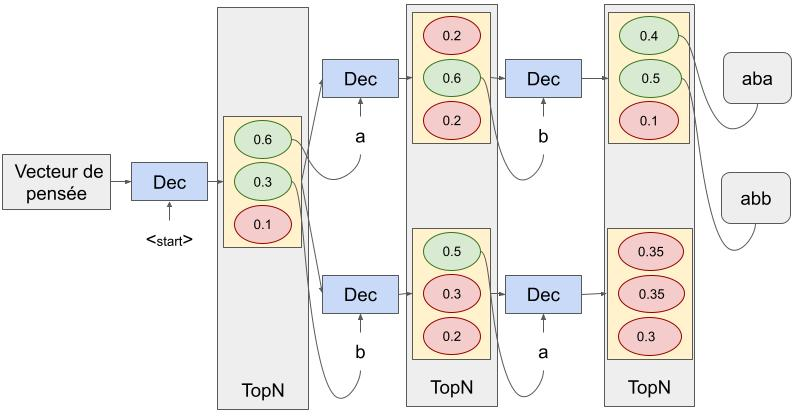
\includegraphics[scale=0.4]{2_production_mots_cles/Beam Search.jpg}
    \caption{Représentation schématique du processus de décodage grâce à l'algorithme de recherche en faisceau.}
    \label{fig:beam_search}
\end{figure}
\todo{refaire en tikz}

\`A l'inverse des algorithmes déterministes que nous avons décrits, notons l'existence des algorithmes d'échantillonnage. Ces algorithmes stochastiques choisissent les mots au hasard en fonction de leur probabilité. Les mots-clés générés par ces algorithmes ne sont donc pas reproductibles, ce qui dans le cadre de la production de mot-clés n'est pas souhaitable. Nous ne considérons donc pas cette technique.

\subsection{Paradigme encodeur-décodeur}\label{sub:paradigme_encodeur_decodeur}

Nous avons présenté dans les sections~\ref{sub:encoding} et \ref{sub:decoding} des moyens d'encoder des documents ainsi que des moyens de générer des séquences.
De nombreuses applications du traitement automatique de la langue nécessitent à la fois l'encodage d'une séquence et son décodage.
Par exemple dans le cadre de la traduction automatique, étant donnée une phrase en langue source, il faut la traduire dans une langue cible, c'est-à-dire qu'il faut encoder la phrase dans la langue source puis générer une phrase correspondante dans la langue cible.
Dans le cadre de la production de mots-clés, il faut générer un mot-clé en fonction d'un document.
Ainsi, le paradigme encodeur-décodeur introduit par \citet{sutskever_sequence_2014}, qui concatène un encodeur et un décodeur, permet de prendre en entrée une séquence de mots de longueur variable et de générer en sortie une autre séquence de mots de longueur variable.
Ce paradigme pallie la limite des réseaux de neurones présentés dans la section~\ref{sub:neural_network} (perceptrons mono ou multicouches) dont l'entrée et la sortie sont de taille fixe.

%Une fois une séquence encodée il est possible de la décoder, c'est-à-dire de produire un mot en fonction d'une représentation $h^t$.
%Générer un mot à partir d'une représentation $h_t$ consiste à passer la représentation dans un perceptron qui calcule une distribution de probabilité sur un vocabulaire, le mot à générer est choisis en fonction de sa probabilité.
    
%\begin{align}
    %\text{log}\: p(y|x) = \sum^m_{j=1} \text{log}\: p(y_j|y_{<j}, x)
%\end{align}

% FROM RECITAL SOTA

\colorlet{enccolor}{green!5}
\colorlet{inputcolor}{black!90!green}
\colorlet{deccolor}{blue!5}
\colorlet{outputcolor}{black!70!blue}
\colorlet{veccolor}{orange!15}
\colorlet{startendcolor}{black!60}
\colorlet{greybox}{black!3}

\begin{figure}[!htb]
\centering

\resizebox{\textwidth}{!}{%
\begin{tikzpicture}

\tikzstyle{cell}=[text centered, rectangle, draw, line width=.5pt, minimum height=1cm, minimum width=1.4cm, rounded corners=2pt]
\tikzstyle{word}=[font=\small\bfseries, text centered, minimum size=.5cm, minimum height=.3cm, text height=1.5ex, text depth=.25ex]
\tikzstyle{vector}=[text centered, rectangle, draw, line width=.5pt, minimum height=.5cm, minimum width=1cm, rounded corners=2pt]
\tikzstyle{arrow}=[shorten >= 2pt, shorten <= 2pt, draw=black!80]

\node[cell, fill=enccolor] (E1) at (0,0){};
\node[cell, fill=enccolor] (E2) at (2,0){};
\node[cell, fill=enccolor] (E3) at (4,0){};
\node[cell, fill=enccolor] (E4) at (6,0){};
\node[text centered] (E5) at (7.5,0){...};
\node[cell, fill=enccolor] (E6) at (9,0){};

\node[word, color=inputcolor, inner color=yellow!50, outer color=white] (I1) at (0,-1.2){Espace};
\node[word, color=inputcolor, inner color=yellow!50, outer color=white] (I2) at (2,-1.2){:};
\node[word, color=inputcolor, inner color=yellow!50, outer color=white] (I3) at (4,-1.2){la};
\node[word, color=inputcolor, inner color=yellow!50, outer color=white] (I4) at (6,-1.2){station};
%\node[word, color=inputcolor, inner color=yellow!50, outer color=white] (I5) at (8,-1.2){...};
\node[word, color=startendcolor] (I6) at (9,-1.2){<fin>};

%\node[cell, fill=veccolor, word, rotate=90] (V) at (11,0){vecteur de pensée};

\node[cell, fill=deccolor] (D1) at (11,0){};
\node[cell, fill=deccolor] (D2) at (13,0){};
\node[cell, fill=deccolor] (D3) at (15,0){};
%\node[cell, fill=deccolor] (D4) at (20,0){};

\node[word, color=startendcolor] (I7) at (11,-1.2){<début>};
\node[word, color=outputcolor, inner color=yellow!50, outer color=white] (O1) at (11,1.2){station};
\node[word, color=outputcolor, inner color=yellow!50, outer color=white] (O2) at (13,1.2){spatiale};
\node[word, color=startendcolor] (O3) at (15,1.2){<fin>};

\draw[->,>=latex,arrow] (E1) -- (E2) node[above,midway] {$h^e_0$};
\draw[->,>=latex,arrow] (E2) -- (E3) node[above,midway] {$h^e_1$};
\draw[->,>=latex,arrow] (E3) -- (E4) node[above,midway] {$h^e_2$};
\draw[->,>=latex,arrow] (E4) -- (E5) node[above,midway] {$h^e_3$};
%\draw[->,>=latex,arrow] (E5) -- (E6) node[above,midway] {$h^e_{n-1}$};
\draw[->,>=latex,arrow] (E5) -- (E6) node[above,midway] {$h^e_{n-1}$};

\draw[->,>=latex,arrow,shorten <= -2pt] (I1) to (E1);
\draw[->,>=latex,arrow,shorten <= -2pt] (I2) to (E2);
\draw[->,>=latex,arrow,shorten <= -2pt] (I3) to (E3);
\draw[->,>=latex,arrow,shorten <= -2pt] (I4) to (E4);
%\draw[->,>=latex,arrow,shorten <= -2pt] (I5) to (E5);
\draw[->,>=latex,arrow,shorten <= -2pt] (I6) to (E6);
\draw[->,>=latex,arrow,shorten <= -2pt] (I7) to (D1);


\draw[->,>=latex, arrow] (E6) -- (D1) node[above,midway] {$h^e_n$};

\draw[->,>=latex,arrow] (D1) -- (D2) node[above,midway] {$h^d_0$};
\draw[->,>=latex,arrow] (D2) -- (D3) node[above,midway] {$h^d_1$};
%\draw[->,>=latex,arrow] (D3) to (D4);

\draw[->,>=latex,arrow,shorten >= -2pt] (D1) to (O1);
\draw[->,>=latex,arrow,shorten >= -2pt] (D2) to (O2);
\draw[->,>=latex,arrow,shorten >= -2pt] (D3) to (O3);
%\draw[->,>=latex,arrow,shorten >= -2pt] (D4) to (O4);

%\node at (5,2) {\large{\textsc{Encodeur}}};
%\node at (17,2) {\large{\textsc{Décodeur}}};

\draw[arrow, rounded corners=3pt] (O1) -| (12, 0);
\draw[->,>=latex, arrow, rounded corners=3pt] (12, 0) -- (12, -1) -| (D2.south);

\draw[arrow, rounded corners=3pt] (O2) -| (14, 0);
\draw[->,>=latex, arrow, rounded corners=3pt] (14, 0) -- (14, -1) -| (D3.south);

%\draw[arrow, rounded corners=3pt] (O3) -| (19, 0);
%\draw[->,>=latex, arrow, rounded corners=3pt] (19, 0) -- (19, -1) -| (D4.south);

\draw[decoration={brace},decorate] (-0.7,1.7) -- node[below=-1.9em] {\large{\textsc{Encodeur}}} (9.7,1.7);
\draw[decoration={brace},decorate] (10.3,1.7) -- node[below=-1.9em] {\large{\textsc{Décodeur}}} (15.7,1.7);


\end{tikzpicture}
}

\caption{Exemple de modèle \textit{encodeur-décodeur} récurrent appliqué à l'extraction automatique de mots-clés.}
\label{fig:seq2seq}
\end{figure}


Le processus d'encodage et de décodage est décrit par l'équation~\ref{eq:enc-dec} et la figure~\ref{fig:seq2seq}.
Dans un premier temps la séquence d'entrée $X$ de taille $n$ est encodée dans le vecteur de pensée $h^e_n$.
Ce vecteur $h^e_n$ est utilisé pour initialiser le premier état caché du décodeur $h^d_0$.
Le décodeur génère ensuite les mots $\hat{y}_t$ qui composent la séquence de sortie $\hat{Y}$ à partir de cet état caché.

\begin{equation}\label{eq:enc-dec}
  \begin{split}
    p(\hat{y}_t | y_{1,...,t-1},h_0) & = \textsc{Softmax}(\sigma(b_v + W_v * h^d_t)) \\
    h^d_t & = \textsc{Rnn}^d(\hat{y}_{t-1}, h^d_{t-1}) \\
    \hat{y}_0 & = \textsc{Debut} \\
    h^d_0 & = h^e_n \\
    h^e_n & = \textsc{Rnn}^e(X) \\
  \end{split}
\end{equation}

Nous présentons ci-après deux améliorations de ce paradigme.
%
D'abord, le mécanisme d'attention qui permet de porter attention à une partie spécifique de l'entrée lors du décodage. Par exemple, la description d'une image nécessite d'identifier les différents objets qui la composent.
%
Ensuite, le mécanisme de copie qui pallie l'incomplétude du vocabulaire de sortie. Ce mécanisme permet au décodeur de copier un mot du document d'entrée au lieu de le générer à partir du vocabulaire de sortie. Le mécanisme de copie est particulièrement utile pour les entités nommées par exemple. Ces entités sont peu fréquentes et ne font généralement pas partie du vocabulaire de sortie.

% Convolution
%Les réseaux de neurones à convolution sont surtout utilisés pour le traitement d'images. Dans le cas du texte, des 
    
% Graphes
%Les réseaux à convolution de graphes (GCN) permettent d'obtenir pour chaque noeud d'un graphe un embedding en fonction de ses voisins. Le nombre de convolutions représente le nombre de bonds qui sont fait entre les noeuds.
    
% Transformer
%Les transformer ont été introduit par \cite{vaswani_attention_2017} et utilisent un mécanisme de self-attention pour chaque mot d'une séquence, de sorte à obtenir pour chaque mot un vecteur qui représente sa relation avec chaque autre mot. Ce mécanisme ne prend pas en compte la séquentialité, en effet chaque calcul est parallélisable. Et ce modèle qui requiert une force de calcul colossale a montré de très bons résultats sur de nombreuse tâches.

\subsubsection{Mécanisme d'attention}
\label{sub:attention_mecanism}

Le mécanisme d'attention~\cite{bahdanau_neural_2014,luong_effective_2015} a été introduit pour améliorer le traitement de longues séquences en permettant au modèle de se focaliser sur certaines parties du document lors du décodage.
%
En effet, un mot-clé concerne seulement certains aspects d'un document. Ce mécanisme permet donc au modèle de porter attention aux parties du document liées à ces aspects.
%
De plus, cette attention au document peut être visualisée grâce aux \emph{poids d'attention} calculés à chaque étape de décodage.
%Par exemple, dans le cadre de la traduction automatique, il permet de visualiser l'alignement entre la phrase en langue source et la phrase en langue cible.
%Par exemple, dans le cadre de la traduction automatique, ce mécanisme permet de visualiser l'importance de chaque mot du document source pour générer la traduction.
La figure~\ref{fig:attention_alignment} illustre cette attention dans le cadre de la traduction automatique pour traduire en français la phrase \say{The agreement on the European Economic Area was signed in August 1992.}
%Il existe généralement un alignement monotone entre les phrases en français et les phrases en anglais.
%Mais ce n'est pas toujours le cas comme le montre le syntagne nominal \say{European Economic Area} dont les mots de la traduction sont dans un ordre inverse \say{zone économique européenne}.
%Le modèle a pu, grâce au mécanisme d'attention, proposer la bonne traduction \say{zone économique européenne} dont l'ordre des mots est inverse à sa traduction.
% Même si le français et l'anglais peuvent généralemnt être traduit mot à mot de manière monotone, le mécanisme d'attention nous permet de visualiser l'alignement non monotone entre zone économique européenne et European Economic Area, en effet l'ordre des noms et adjectifs en français et en anglais est différent.
%Ainsi nous pouvons observer que pour traduire \say{was} en \say{a été}, le modèle à porté attention à \say{was signed} pour comprendre que \say{was} fait parti de la construction du prétérit.
%Pour illustrer ce mécanisme dans le cadre de la traduction automatique nous prenons l'exemple suivant: pour traduire la séquence \say{the European Economic Area} en français (\say{\foreign{la zone économique européenne}}) le modèle portera attention à chaque mot du texte source. Ainsi, pour générer \say{la} et \say{zone} il devra porter attention à \say{\foreign{the}} et \say{\foreign{Area}}. \todo{A revoir.}

\begin{figure}
    \centering
    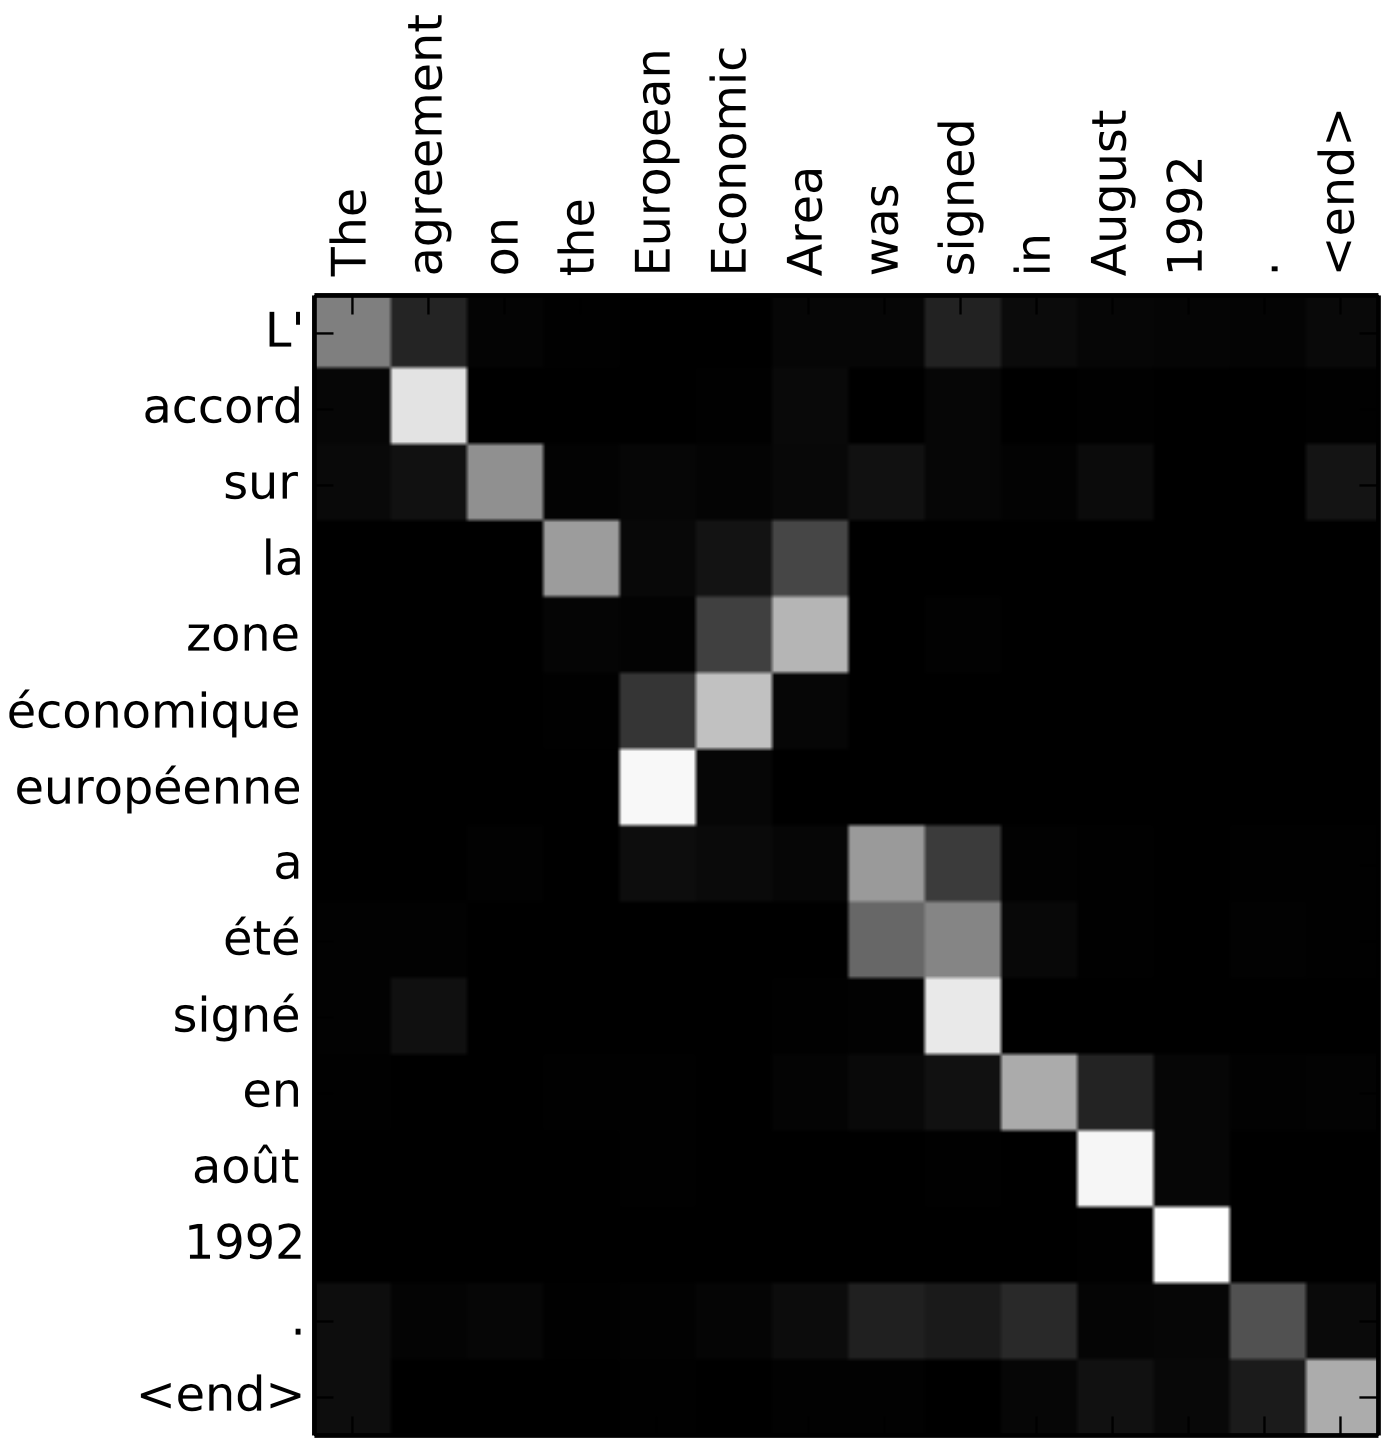
\includegraphics[scale=0.3]{2_production_mots_cles/attention_alignment.png}
    \caption{Exemple de visualisation des poids d'alignement du mécanisme d'attention entre une phrase en anglais et sa traduction en français. Chaque ligne montre la distribution des poids $\alpha_{t}$ ayant servis à générer le mot correspondant en français. Une case blanche indique un poids de 1, une case noire indique un poids de 0. Image extraite de \citet{bahdanau_neural_2014}.}
    \label{fig:attention_alignment}
\end{figure}

%Il faudra aussi porter attention à la syntaxe des deux langues
%Les poids d'attention peuvent être utilisés pour visualiser l'alignement entre les mots de la séquence d'entrée et ceux de la séquence de sortie.
%La figure~\ref{fig:attention_alignment} montre les poids d'alignement dans le cadre de la traduction automatique entre une phrase en anglais et sa traduction en français.

Le décodeur utilise l'état caché courant $h^d_t$ pour générer un mot, le mécanisme d'attention lui permet d'utiliser aussi tous les états cachés de l'encodeur $h^e$ pour mettre à jour l'état caché du décodeur $h^d_t$. Ce mécanisme est décrit dans l'équation~\ref{eq:attention}.
Dans le mécanisme d'attention, les états cachés $h^e$ sont pondérés en fonction de leur importance pour générer le mot $\hat{y}_t$.
Cette importance est établie grâce à une fonction d'alignement $a$ qui calcule une similarité entre l'état caché courant $h^d_t$ et ceux de l'encodeur $h^e$.
Les états cachés $h^e$ sont ainsi moyennés dans le vecteur de contexte $c_t$ utilisé pour mettre à jour l'état caché courant du décodeur $h^d_t$.

Dans l'équation \ref{eq:attention}: $[u;v]$ représente l'opération de concaténation des vecteurs $u$ et $v$; $a$ est une fonction d'alignement qui calcule la similarité entre un état caché de l'encodeur $h^e_t$ et du décodeur $h^d_t$; $\alpha$ représente les poids d'alignement entre les états cachés de l'encodeur $h^e$ et du décodeur $h^d$;  et $\textsc{Softmax}$ est une fonction qui normalise les valeurs d'un vecteur pour qu'il somme à 1.


\iffalse
    \begin{figure}
        \centering
        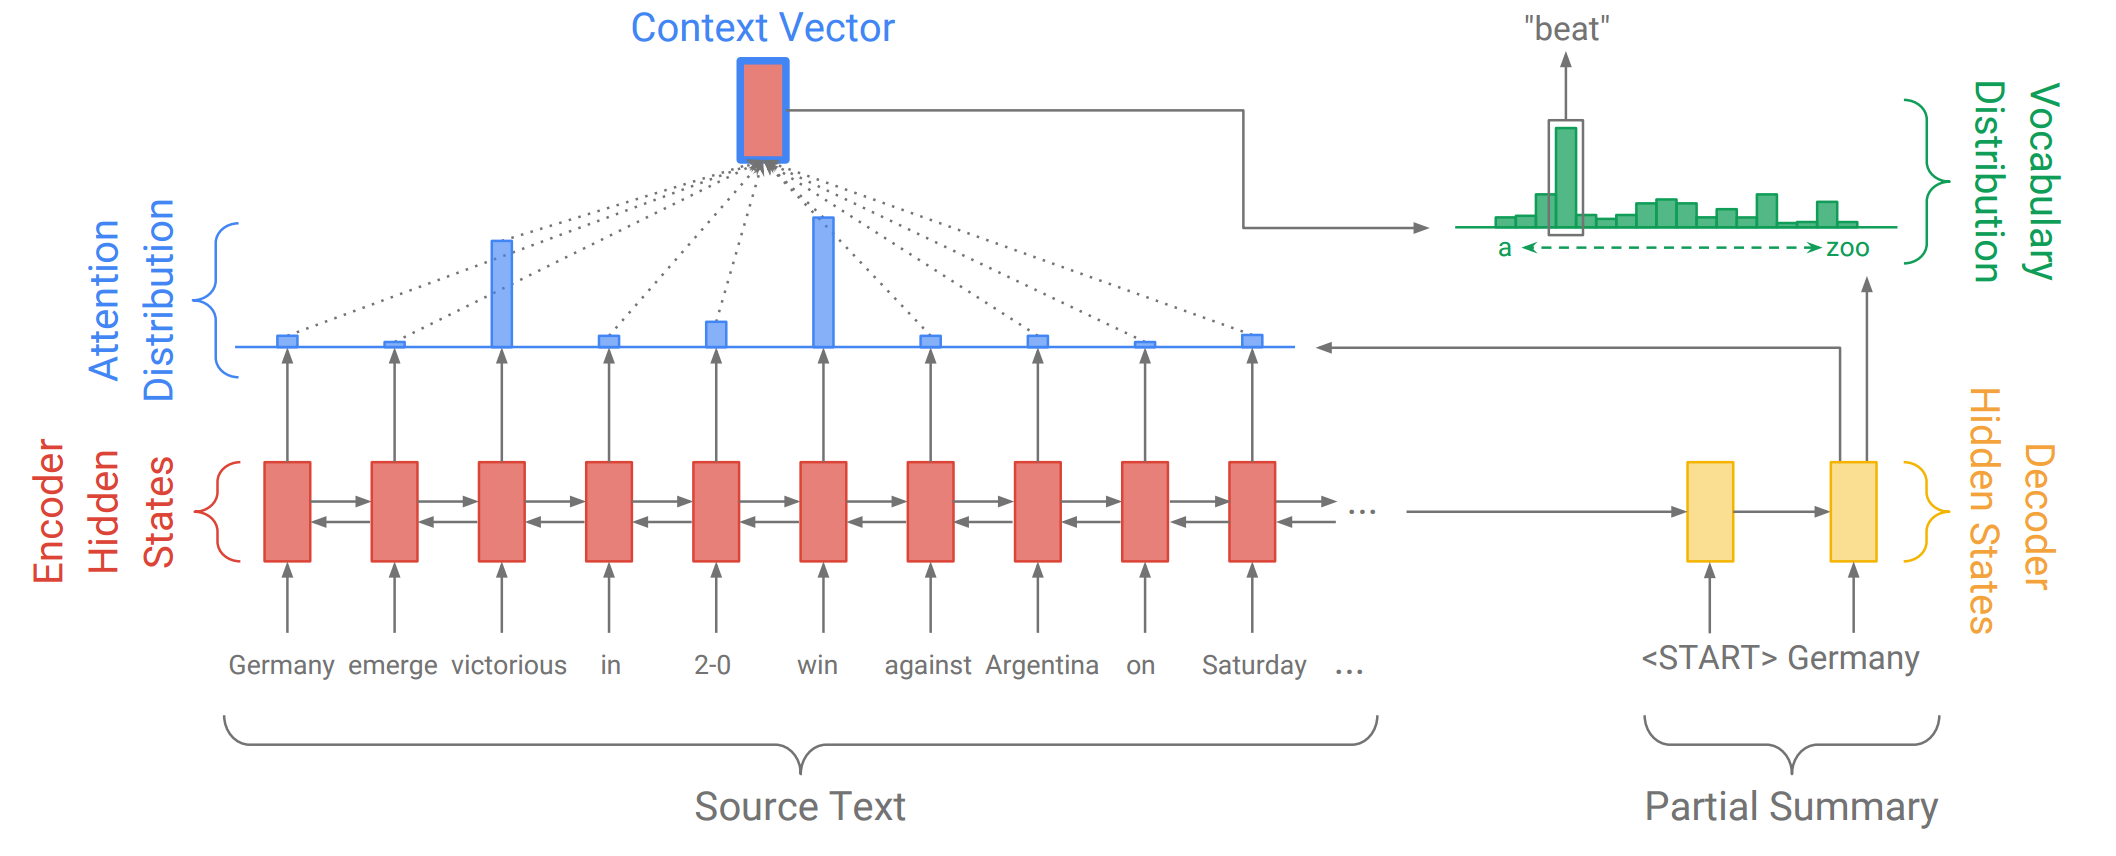
\includegraphics[width=\linewidth]{figures/see_seq2seq-attn.png}
        \caption{Schéma du mécanisme de copie présenté par \cite{see_get_2017}.}
        \label{fig:see_attention}
    \end{figure}
\fi

\begin{equation}\label{eq:attention}
  \begin{split}
    %\hat{Y}_t & = \sigma(b_v + W_v * h^d_t) \\
    p(y_t|y_{<t},x) & = \textsc{Softmax}(\sigma(W_v h^d_t)) \\[.3em]
    h^d_t & = \textsc{Rnn}(y_{t-1}, [h^d_{t-1};c_t]  \\[.3em]
    c_t & = \sum^{|h^e|}_{i=0} \alpha_{i,t} h^e_i \\
    \alpha_{t} & = \textsc{Softmax}(a(h^d_t, h^e)) \\
    %\textsc{Softmax}(x) & = \left[ \frac{x_i}{\sum^{|x|}_{i=0} x_i} , i \in |x| \right]
  \end{split}
\end{equation}

%Le concept d'attention a été présenté de deux manières différentes par \cite{bahdanau_neural_2014} et \cite{luong_effective_2015}.
%
%L'idée de l'attention présentée par~\cite{luong_effective_2015} est \emph{d'utiliser le vecteur de contexte pour prédire $y_t$}.
%
%\cite{bahdanau_neural_2014} présente un autre mécanisme d'attention dont l'idée est de calculer l'état caché du décodeur à l'aide d'un vecteur de contexte. Par rapport à un décodeur classique, seul le calcul de $h^d_t$ change.

\iffalse
    L'idée de l'attention présentée par~\cite{luong_effective_2015} est \emph{d'utiliser le vecteur de contexte pour prédire $y_t$}.
    
    Pour cela, un nouveau $\hat{h}^d_t$ est calculé en fonction d'un vecteur de contexte $c_t$ et de $h^d_t$ (calculé en fonction de $y_{t-1}$ et $h^d_{t-1}$). $c_t$ est la moyenne des $h^e$ pondérés par les scores d'alignement $\alpha$.
    
    Dans leur article, deux manières de calculer l'attention sont présentées: une attention globale et une attention locale.
    %
    Pour l'attention globale, le vecteur de contexte est la moyenne pondérée de toutes les représentations de l'encodeur.
    %
    Pour l'attention locale, le vecteur de contexte est la moyenne pondérée des représentations $h^e$ dans une fenêtre de taille $D$ autour de $h^e_{p_t}$.
    %
    $p_t$ est une valeur entre 0 et $|h^e|$ qui définit le centre de la fenêtre, et peut être calculé de différentes manières.\footnote{Pour plus de détails voir la section 3.2 de \cite{luong_effective_2015}}
    %$p_t$ étant $t$ (dans la traduction automatique on considère que le mot cible $y_t$ est aligné avec le mot source $x_{p_t}$), ou alors un réel entre 0 et $|h^e|$ calculé à l'aide 
    
    \begin{align}
        %y_t & = \sigma(W_v h^d_t) \\
        p(y_t | y_{<t}, x) & = \textsc{Softmax}(W_v \hat{h}^d_t) \\
        \hat{h}^d_t & = \sigma(W_c [c_t;h^d_t]) \\
        c_t & = \sum^{|h^e|}_{i=0} \alpha_{i,t} * h^e_i \\
        \alpha_{i,t} & = \textsc{Softmax}(a(h^e_i, h^d_t)) \\
        h^d_t & = \textsc{Rnn}(y_{t-1}, h^d_{t-1})
    \end{align}
    
    \cite{bahdanau_neural_2014} présente un autre mécanisme d'attention dont l'idée est de calculer l'état caché du décodeur à l'aide d'un vecteur de contexte. Par rapport à un décodeur classique, seul le calcul de $h^d_t$ change. Le calcul du vecteur de contexte est similaire à celui de ~\cite{luong_effective_2015}.
    
    \begin{align}
        p(y_t|y_{<t},x) & = \textsc{Softmax}(W_v h^d_t) \\
        h^d_t & = \textsc{Rnn}(y_{t-1}, [h^d_{t-1};c_t]  \\
        c_t & = \sum^{|h^e|}_{i=0} \alpha_{i,t} * h^e_i \\
        \alpha_{i,t} & = \textsc{Softmax}(a(h^e_i, h^d_t))
    \end{align}
    
    Il existe différentes fonctions d'alignement:
    
    bahdanau $a(h^e_i, h^d_t) = v_a \text{tanh}(W_a h^d_t + U_a h^e_i)$
    
    dot $a(h^e_i, h^d_t) = h^e_i h^d_t$
    
    general $a(h^e_i, h^d_t) = h^e_i W_a h^d_t$
    
    concat $a(h^e_i, h^d_t) = W_a [h^e_i;h^d_t]$
\fi

\subsubsection{Mécanisme de copie}
\label{sub:copy_mecanism}

Le mécanisme de copie~\cite{see_get_2017,gu_incorporating_2016} provient des tâches de traduction automatique et de résumé automatique. Il a pour but de produire des mots peu fréquents ou hors du vocabulaire de sortie.
En effet, les modèles neuronaux qui génèrent du texte choisissent les mots dans un vocabulaire de sortie comportant généralement \num{50 000} mots.
Dans les tâches sus-citées, les mots peu fréquents qui ne font pas partie du vocabulaire de sortie, comme les entités nommées ou les transfuges, doivent pourtant apparaître dans la séquence de sortie.
%Le mécanisme de copie ~\cite{see_get_2017,gu_incorporating_2016} pallie ce problème en permettant au décodeur de générer un mot du vocabulaire de sortie ou bien de copier un mot du document.
Deux mécanismes de copie ont été proposés par \citet{see_get_2017} et \citet{gu_incorporating_2016}; les deux étant similaires, nous présentons ici le premier car plus simple. Il est décrit dans l'équation~\ref{eq:copy_mecanism}.

% exemple
%Le mécanisme d'attention a été utilisé comme post-traitement pour remplacer les mots inconnus de la sortie par les mots de l'entrée alignés par le mécanisme d'attention. Ceci permettant de traiter les entités nommées peu fréquentes ou les transfuges.
%
%Le mécanisme de copie vient automatiser ce processus en permettant au modèle de générer un mot du vocabulaire ou de copier un mot du document.

%, tous deux inspirés des réseaux de pointeurs~\cite{vinyals_pointer_2015} qui génèrent une séquence de pointeurs vers la séquence d'entrée.
Ce mécanisme utilise le vocabulaire de la séquence d'entrée $\mathcal{X}$ (particulier à chaque document) en plus du vocabulaire de sortie $\mathcal{V}$.
Pour produire un mot, une distribution de probabilité sur le vocabulaire  $P_{vocab}(y_{t})$ est calculée comme précédemment par le décodeur (cf. section~\ref{sub:decoding}) et les poids du mécanisme d'attention $\alpha$ (cf. section~\ref{sub:attention_mecanism}) sont utilisés pour estimer la probabilité de copie de chaque mot du document.
Les poids d'attention $\alpha$ des mots qui apparaissent plusieurs fois dans l'entrée $x$ sont sommés $\sum_{j,x_j=y_{t,i}} \alpha^t_j$.
Ainsi, un mot peut être généré à partir du vocabulaire de sortie $\mathcal{V}$ ou copié à partir du vocabulaire du document $\mathcal{X}$.
Les probabilités de copie et de génération d'un même mot, qui appartient au document et au vocabulaire, sont sommées.
Dans l'équation~\ref{eq:copy_mecanism}: $h^d_t$, $c_t$ et $\alpha^t_j$ proviennent du mécanisme d'attention (cf. équation~\ref{eq:attention}); $p_{gen}$ est un curseur permettant au modèle de privilégier la copie ou la génération et $P_{vocab}(y_t)$ est une distribution de probabilité sur le vocabulaire de sortie $\mathcal{V}$.

%Les probabilités de génération et de copie sont combinés pour donner une distribution de probabilités sur $\mathcal{X} \cup \mathcal{V}$.

\begin{equation}\label{eq:copy_mecanism}
  \begin{split}
    p(y_{t,i}|y_{<t},x) & = p_{gen} P_{vocab}(y_{t,i}) + (1 - p_{gen}) \sum_{j,x_j=y_{t,i}} \alpha^t_j \\
    p_{gen} & = \sigma(W_h h^d_t + W_c c_t + W_y y_{t-1}) \\
    P_{vocab}(y_{t}) & = \textsc{Softmax}(\sigma(W_v h^d_t))
  \end{split}
\end{equation}

%ou les poids d'un mécanisme d'attention supplémentaire, utilisé seulement pour calculer le score de copie, pour~\cite{gu_incorporating_2016}

\iffalse
    %\cite{gu_incorporating_2016}, création d'un vocabulaire spécifique a chaque instance, composé de $\mathcal{V}$ le vocabulaire normal et $\mathcal{X}$ le vocabulaire des mots de l'entrée.
    %
    %Ça change le calcul de $y_t$ par rapport au mécanisme d'attention.
    %
    %On défini les vecteurs $\psi_g \in \mathds{R}^|\mathcal{V}|$ et $\psi_c \in \mathds{R}^|\mathcal{X}|$ qui contiennent respectivement les score de copie et de génération.
    
    % attentive read = les poids de l'attention
    % selective read = les poids de l'"attention" du mécanisme de copie
    
    \begin{align}
        y_t & = \textsc{Softmax}(e^{P_{gen}} +e^{P_{copy}}) \\
        P_{gen} & = W_v h^d_t \\
        P_{copy} & = \left[ \sum^{|h^e|}_{j=0, x_j=x_i} \sigma(h^e_j W_c) h^d_t | x_i \in \mathcal{X} \right] \\
        h^d_t & = RNN([y_{t-1};cc_t)],h^d_{t-1}) \\
        cc_t & = \sum^{|h^e|}_{i=1} aa_{t,i} h^e_t \\
        aa_{t,i} & = \textsc{Softmax}()
    \end{align}
    
    %\cite{see_get_2017} reprend le mécanisme d'attention de \cite{luong_effective_2015} et modifie le calcul de $y_t$ en ajoutant une probabilité de copie et un curseur privilégiant la copie ou la génération.
    
    \begin{align}
        p(y_{t,i}) = p_{gen} P_{vocab}(y_{t,i}) + (1 - p_{gen}) \sum_{j,x_j=y_{t,i}} \alpha^t_j \\
        p_{gen} = \sigma(W_c c_t + W_h h^d_t + W_y y_{t-1})
    \end{align}
\fi

% Multitache
% Conditional Random Field
% Reinforcement Learning : adaptative reward


\section{Méthodes de bout-en-bout}
\label{methodes-de-bout-en-bout}

\todo{Ajouter des schéma pour mieux comprendre les méthodes.}

Dans cette section nous présentons un état de l'art des méthodes de bout-en-bout.
Ces méthodes, contrairement aux méthodes en chaîne de traitement (cf. section~\ref{sec:methode-en-chaine-de-traitement}), prennent en entrée un document et laissent le soin au modèle d'en extraire les caractéristiques pour retourner un ensemble de mots-clés sans étapes intermédiaires ni définition manuelle de ces caractéristiques.
Parmi les méthodes proposées dans la littérature, nous distinguons les méthodes génératives, qui peuvent produire des mots-clés présents et des mots-clés absents, des méthodes extractives, limitées aux mots-clés présents.

Jusqu'à présent, toutes les méthodes de bout-en-bout qui ont été proposées sont supervisées et reposent sur des réseaux de neurones (cf. section~\ref{sub:neural_network}) qui nécessitent de grandes quantités de données annotées pour être entraînées.
%
Le développement de ces méthodes démarre avec l'introduction du jeu de données KP20k et de la méthode générative CopyRNN par \citet{meng_deep_2017}.
Le jeu de données KP20k, qui comporte $\simeq$\num{550000} documents, comble un manque.
En effet, seuls de petits jeux de données (de l'ordre du millier de documents) étaient jusqu'alors disponibles.
Ce travail a ainsi lancé une nouvelle direction de recherche sur les méthodes génératives de production de mot-clés.

\begin{figure}
    \centering
    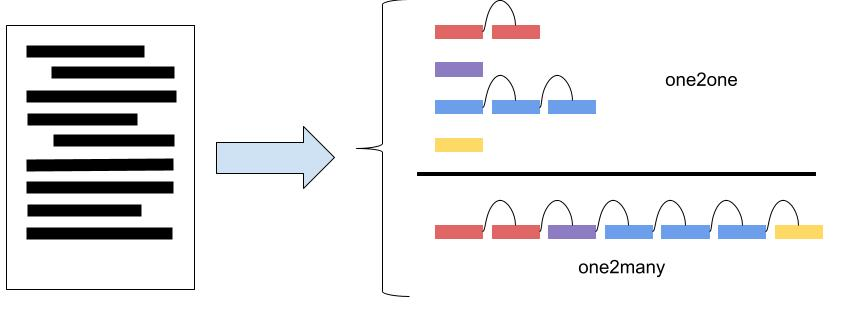
\includegraphics[scale=0.4]{2_production_mots_cles/Decoding strategies.jpg}
    \caption{Représentation schématique des stratégies de décodage \emph{one2one} et \emph{one2many}.}
    \label{fig:decoding_strategies}
\end{figure}
\todo{Refaire en tikz}

Dans cet état de l'art, nous présentons tout d'abord les méthodes automatiques de génération de mots-clés de bout-en-bout, qui sont au c\oe{}ur de ce travail de thèse.
Nous présentons ces méthodes de génération en deux parties: premièrement, les méthodes qui générent les mots-clés un à un (\emph{one2one}), et deuxièmement, celles qui génèrent des séquences de mots-clés (\emph{one2many}). Ces deux types de génération sont schématisés dans la figure~\ref{fig:decoding_strategies}.
Nous présentons ensuite les méthodes extractives de bout-en-bout, c'est-à-dire celles qui se limitent aux seuls mots-clés présents.

\subsection{Génération de mots-clés}
\label{sub:generation_de_mots_cles}

Les méthodes génératives, introduites par \citet{meng_deep_2017}, ont pour objectif de pallier deux faiblesses qui concernent la majorité des méthodes extractives présentées précédemment: l'impossibilité de produire des mots-clés absents ainsi que la faible prise en compte de la sémantique.
Le paradigme encodeur-décodeur sur lequel les méthodes génératives sont fondées permet d'encoder la sémantique du document.
Ainsi, les mots-clés produits sont le fruit d'une \say{compréhension} du document, contrairement aux méthodes en chaîne de traitement qui s'intéressent à l'\say{importance} des mots dans le document indépendamment de leur sens.
%
Ces méthodes génératives rendent possible la production de mots-clés absents grâce à la manière dont le décodeur génère la séquence de sortie.
Ce processus s'effectue en choisissant, à chaque étape de décodage, un mot à partir d'un vocabulaire de sortie qui est plus grand et différent du vocabulaire du document.
Ces méthodes génératives apprennent à générer des mots-clés un par un (génération \emph{one2one}, voir figure~\ref{fig:decoding_strategies}), c'est-à-dire que chaque document $X$ et son ensemble de mot-clés $Y$ de taille $N$ forment un couple $(X, \{Y_0, ..., Y_N\})$, décomposé en autant d'exemples d'entraînement que de mots-clés, $(X, Y_0), ... , (X, Y_N)$.

%\paragraph{Définitions}
%\todo{Il faudrait définir avant les principaux modèles: one2one, séquence avant de les définir formellement; Fait ausi des dessins}
%$x$ et $y$ représentent des mots, $p$ des mots-clés. Étant donné un ensemble de données $D = {(x^i,p^i), i \in 1...N}$ de taille $N$, un exemple est composé d'un document $x^i$ et d'un ensemble de mots-clés $p^i = {p^i_j, j \in 1...M^i}$ de taille $M^i$. Les documents et les mots-clés sont composés de mots $[x^i_k, k \in 1...N^i]$ et $[y^i_j]$ est composé d'un document composé d'une séquence de mots $x^i = (x^i_1, ..., x^i_{N^i})$ de longueur $N^i$ et d'un ensemble de mots-clés $p^i$ de taille $M^i$ avec $p^i = (p^i_1, ..., p^i_{M^i})$, où chaque mot-clé est une séquence de mots de taille $M^{i,j}$ avec $p^{i,j} = (y^{i,j}_1, ..., y^{i,j}_{M^{i,j}})$. Dans le cadre des modèles one2one, un couple document -- mots-clés est découpé en $M^i$ différents couples $(x^i, p^{i,1}), ..., (x^i, p^{i, M^i})$. 
%Pour les modèles en séquences, les mots-clés sont concaténés de sorte à former une unique séquence $(x^i, y^{i,1}_1 \lozenge ... \lozenge y^{i,1}_{M^{i,j}} \lozenge \text{SEP} \lozenge y^{i,2}_1 \lozenge ... \lozenge y^{i,M^i}_{M^{i,j}})$.

La méthode pionnière de génération automatique de mots-clés appliquée aux documents scientifiques est CopyRNN~\cite{meng_deep_2017}.
%
L'architecture neuronale de cette méthode s'inspire du processus d'annotation humain qui consiste à lire le document pour le comprendre dans son entièreté puis à le résumer grâce à des mots-clés.
%Aussi, les humains peuvent facilement s'abstraire du texte et faire appel à leurs connaissances pour produire des mots-clés qui n'apparaissent pas dans le texte.
Pour reproduire ce processus, CopyRNN utilise le paradigme encodeur-décodeur, que nous avons présenté dans la section~\ref{sub:paradigme_encodeur_decodeur}, pour encoder un document et le décoder ensuite en un mot-clé. % Ainsi un réseau de neurones récurrent encode le document dans un vecteur de pensée, puis un autre décode, génère, ce vecteur de pensée en un mot-clé.
Pour améliorer les performances des modèles encodeur-décodeur, il est commun d'utiliser un mécanisme d'attention (voir section~\ref{sub:attention_mecanism}).
Ce mécanisme permet au modèle de porter attention à certaines parties du document lors de la génération d'un mot.
%
Un mécanisme de copie est aussi ajouté au modèle pour lui permettre de générer des mots peu fréquents (voir section~\ref{sub:copy_mecanism}).
Ce mécanisme de copie modifie le décodage en permettant de générer un mot à partir du vocabulaire de sortie ou bien à partir du document.\\
%
Cette méthode obtient des performances bien plus élevées que les précédentes méthodes extractives. Les performances de CopyRNN sont de l'ordre de 30 points de \fmesure{} pour les mots-clés présents tandis que les performances des méthodes extractives sont généralement en dessous de 20 points de \fmesure{}.
Les mots-clés absents, qui ne pouvaient jusque-là pas être produits, correspondent peu à la référence: parmi les 50 meilleurs mots-clés absents un seul apparaît dans la référence.


%La communauté scientifique présente de nouvelles méthodes basées sur CopyRNN et tente de l'améliorer.
% les méthodes essaient de résoudre les problèmes identifiés
%Les méthodes présentées augmentent toujours les performances de génération des mots-clés présents et absents.

Certaines méthodes proposées essaient d'améliorer l'encodage du document.
\citet{chen_title-guided_2019}, par exemple, constate que les mots-clés ne sont pas uniformément distribués dans les documents.
En particulier \npercent{60} des mots-clés de référence ont au moins un mot en commun avec le titre du document.
Pour prendre cela en compte, ils proposent TGNet (Title Guided Network), qui étend CopyRNN en introduisant un nouvel encodeur spécifique au titre, en plus de l'encodeur du document.
Cet encodage du titre permet de donner un poids supplémentaire à l'information qu'il contient.
Ces deux représentations (du titre et du document) sont ensuite combinées puis fournies au décodeur.
Cette méthode améliore nettement les performances de génération des mots-clés présents et absents par rapport à CopyRNN (+\npercent{5} sur KP20k).
% Ils ne regardent que la F-mesure présent/absent rien d'autre

La redondance dans les ensembles de mots-clés produits est un problème récurrent dans les méthodes de production de mots-clés.
En effet, \citet{hasan_automatic_2014} montrent que 8 à \npercent{12} des erreurs des méthodes sont liées à la redondance des mots-clés.
Ainsi, les méthodes en chaîne de traitement mettent en place des stratégies, notamment lors de la sélection du sous-ensemble de mots-clés, pour limiter cette redondance (voir section~\ref{choisir-le-sous-ensemble}).
Dans cette ligne de recherche, \citet{zhao_incorporating_2019} remarquent les méthodes de bout-en-bout ne sont pas exemptes de ce problème, ils s'intéressent ainsi au chevauchement entre les mots-clés générés et ceux de référence.
Par exemple, \npercent{23.98} des mots-clés unigrammes générés par CopyRNN font partie d'un mot-clé de référence, et \npercent{47.15} des mots-clés 4-grammes générés par CopyRNN contiennent un mot-clé de référence.
Dans l'optique de limiter ces chevauchement, ils présentent le modèle ParaNet$_T$+CoAtt qui entraîne le modèle, à générer à la fois les mots-clés et leurs étiquettes morphosyntaxiques, ainsi la syntaxe des mots-clés générés sera similaire à celle des mots-clés de référence.
Pour cela ils ajoutent au modèle CopyRNN un encodeur, pour les étiquettes morphosyntaxiques des mots du document, ainsi qu'un décodeur, pour celles du mot-clé.\footnote{Les étiquettes morphosyntaxiques du document et des mots-clés proviennent de l'outils Stanford CoreNLP.}
Les informations des deux décodeurs sont ensuite combinées et utilisées pour générer les mots-clés et leurs étiquettes morphosyntaxiques.
%Grâce à cette méthode, les mots-clés générés chevauchent moins les mots-clés de référence; par exemple le pourcentage de mot-clés 4-grammes contenant un mot-clé de référence a baissé de \npercent{10}.

\begin{figure}
    \centering
    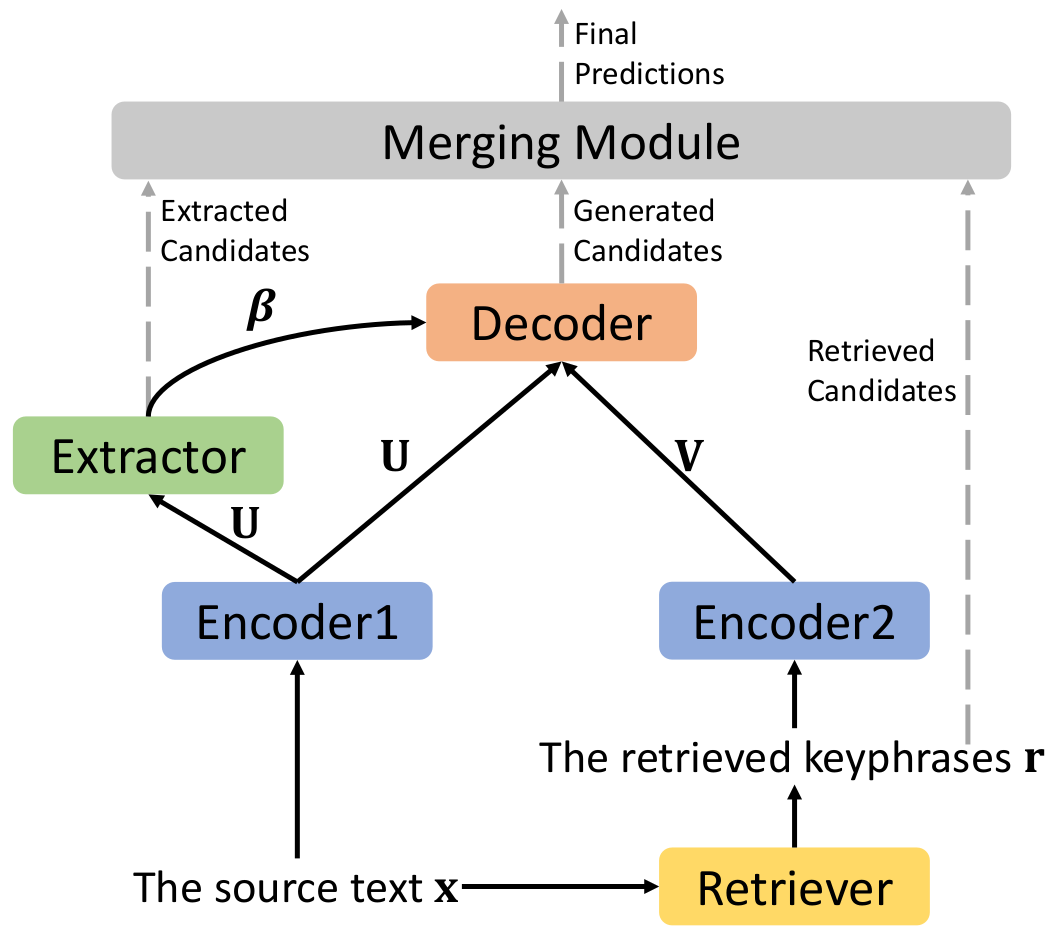
\includegraphics[scale=0.2]{2_production_mots_cles/kg_ke_kr_m.png}
    \caption{Représentation schématique de l'architecture de la méthode KG-KE-KR-M. Image extraite de~\citet{chen_integrated_2019}.}
    \label{fig:schema_kgkekrm}
\end{figure}

%Le processus manuel d'annotation en mots-clés est composé de plusieurs étapes: la lecture du document, l'extraction des mots-clés dans le document puis l'attribution de mots-clés absents du document et enfin la combinaison des mots-clés provenant de ces deux processus d'annotation.
Dans l'optique de reproduire l'annotation humaine, \citet{chen_integrated_2019} propose la méthode KG-KE-KR-M qui produit un ensemble de mots-clés en combinant différentes méthodes: génération de mots-clés, extraction de mots-clés, récupération de mots-clés (voir figure~\ref{fig:schema_kgkekrm}).
%Ces différentes méthodes sont entraînées de bout-en-bout puis les mots-clés de chaque méthode sont pondérés grâce à un classifieur.
%
Dans un premier temps, cette méthode récupère les mots-clés de référence des $K$ documents d'entraînement les plus proches du document traité (grâce à la distance de Jaccard).
Ces mots-clés \emph{récupérés} sont concaténés puis encodés. Ils serviront à conditionner la génération de mots-clés.
Dans un second temps, des mots-clés sont \emph{extraits} du document en classifiant chaque mot comme mot-clé ou non mot-clé.
%Cette classification s'effectue grâce aux états cachés du document encodé.
Ensuite, des mots-clés sont \emph{générés} à partir du document ainsi que des mots-clés récupérés et des mots-clés extraits.
Enfin, les mots-clés récupérés, extraits et générés sont pondérés grâce à un classifieur.
Cette méthode à la particularité de combiner les méthodes en chaîne de traitement (sélection de candidats puis pondération) et les méthodes de bout-en-bout (apprentissage conjoint de la génération et de l'extraction).
Malgré la grande diversité dans les techniques de production de mots-clés candidats, les performances ne sont pas significativement supérieures à CopyRNN. Cette méthode produit néanmoins plus de mots-clés absents de référence que CopyRNN.

La méthode CorrRNN~\cite{chen_keyphrase_2018} considère que les mots-clés doivent couvrir l'ensemble des sujets du document et être divers, c'est-à-dire que chaque mot-clé doit concerner un sujet différent.
Cette méthode étend CopyRNN en y ajoutant un mécanisme de couverture et un mécanisme de revue.
Le mécanisme de couverture encourage le modèle à porter attention aux différentes parties du document.
Il conserve et accumule les scores d'attention des mots du document à chaque étape de décodage, et il est inclus dans le calcul du mécanisme d'attention.
Ensuite, le mécanisme de revue est essentiellement un mécanisme d'attention sur les mots générés.
Son objectif est d'identifier les sujets déjà couverts par les mots-clés générés et ainsi de générer des mots-clés qui concernent des sujets non traités.
Cette méthode est la première à prendre en compte les mots-clés déjà générés dans le processus de génération, pour cela la phase d'entraînement est modifiée.
Au lieu de rétro-propager le gradient après chaque mot-clé de référence, la phase de rétro-propagation n'est effectuée qu'une fois tous les mots-clés de référence du document traités.
%Chaque mot-clé est généré en utilisant les mécanismes de couverture et de redondance, qui prennent en compte les mots-clés déjà générés; le gradient est ensuite calculé grâce à l'erreur de chaque mot-clé; et enfin, rétro-propagé.
%Cette méthode améliore les performance de production de mots-clés présent par rapport à CopyRNN, mais l'article ne présentant pas ses résultats sur le jeu de données de référence KP20k et utilisant des métriques peu utilisés dans les autres travaux la comparaison est limitée.

\subsection{Génération de séquences de mots-clés}% (\textsc{One2Seq})}
%\subsection{Génération en séquence}
\label{sub:generation_de_sequences_de_mots_cles}

%Nous avons présenté dans la section précédente, des méthodes génératives qui apprennent à générer un mot-clé par document.
Nous présentons dans cette section des méthodes qui apprennent à générer des séquences de mots-clés (génération \emph{one2many}, voir figure~\ref{fig:decoding_strategies}). C'est-à-dire que chaque exemple d'entraînement est composé d'un document et de la concaténation des mots-clés de référence en une unique séquence dans laquelle ils sont séparés par un symbole de séparation. Par exemple, l'ensemble de mots-clés $\{$ Classe , Fichier log , Agrégat $\}$ sera transformé en \say{Classe \texttt{SEP} Fichier log \texttt{SEP} Agrégat \texttt{FIN}}.
%Le développement des méthodes utilisant la génération \emph{one2many} part du constat que la génération \emph{one2one} ne permet pas de prendre en compte les mots-clés déjà générés et que les ensembles de mots-clés sont souvent redondants~\cite{hasan_automatic_2014}.
Le développement des méthodes génératives \emph{one2many} part du constat que les ensembles de mots-clés produits sont souvent redondants~\cite{hasan_automatic_2014} et que la génération \emph{one2one} ne permet pas de pallier ce problème.
En effet, les méthodes \emph{one2many} font l'hypothèse qu'avec la génération en séquence, le modèle ayant accès aux mots-clés déjà générés, il ne générera pas de mots-clés redondants.
%
Cette méthode de génération permet au modèle de générer le même nombre de mots-clés que la référence, en effet, il apprend en même temps qu'à générer les mots-clés, à placer les séparateurs de mots-clés et le symbole de fin.
Ainsi, ces méthodes peuvent générer des mots-clés selon deux stratégies~\cite{yuan_one_2020}: l'\textbf{inférence exhaustive} qui utilise l'algorithme de recherche en faisceau pour sur-générer des mots-clés et ainsi en obtenir un nombre fixe pour chaque document, c'est la stratégie employée par les méthodes génératives \emph{one2one}; et l'\textbf{inférence auto-régulée} (\foreign{self-terminating}) dans laquelle le décodage s'arrête lors de la génération du symbole de fin, cette stratégie permet au modèle de produire un nombre pertinent de mots-clés pour le document.
La seconde stratégie de décodage permet donc de s'affranchir du choix arbitraire du nombre de mots-clés $n$ à produire (voir section~\ref{choisir-le-sous-ensemble}).

Pour entraîner ces modèles, les mots-clés sont concaténés, mais ce processus n'est pas trivial.
En effet, l'ordre dans lequel les mots-clés sont concaténés influence les performances des modèles.
L'étude de \citet{meng_empirical_2021} compare différentes manières d'ordonner les mots-clés, telles que: \emph{No-Sort} qui laisse l'ordre par défaut; \emph{Alpha} qui trie par ordre alphabétique; \emph{Pres-Abs} qui place les mots-clés présents avant les mots-clés absents. L'étude montre que c'est l'ordre \emph{Pres-Abs} qui donne les meilleures performances.

La première méthode à générer des séquences de mots-clés est catSeqD~\cite{yuan_one_2020,yuan_generating_2018}.
L'objectif de cette méthode, similaire à CorrRNN, est d'augmenter la diversité des mots-clés générés.
%
Pour cela, le modèle CopyRNN, utilisé comme base, est augmenté d'un mécanisme de couverture sémantique et de régularisation orthogonale pour former le modèle catSeqD.
%
Le mécanisme de \emph{couverture sémantique} repose sur l'hypothèse que l'ensemble de mots-clés de référence et le document encodent la même information.
Ainsi, un nouvel encodeur est entraîné à encoder les mots-clés et à produire la même représentation que pour le document.
Il encode la séquence au fur et à mesure de sa génération et l'état cachés qui en résulte conditionne la prédiction du mot suivant, cela contraint les mots-clés générés à être proche sémantiquement du document.
%
Ensuite, les auteurs constatent que les mots générés après les séparateurs de mots-clés sont souvent similaires.
Le mécanisme de \emph{régularisation orthogonale} pallie ce problème en diversifiant explicitement les représentations des séparateurs, en pénalisant, dans la fonction de coût, ces représentations si elles ne sont pas orthogonales.

\todo{Refaire en Tikz}
\begin{figure}
    \centering
    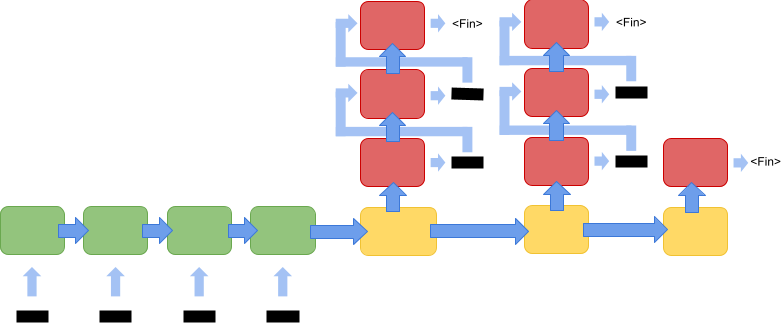
\includegraphics[scale=0.5]{2_production_mots_cles/exhird.png}
    \caption{Représentation schématique du décodage hiérarchique de la méthode ExHirD. L'encodeur du document est représenté en vert, le décodeur de concept en jaune et le décodeur de mots-clés en rouge.}
    \label{fig:schema_exhird}
\end{figure}

Dans le but de mieux modéliser les ensembles de mots-clés, \citet{chen_exclusive_2020} s'intéressent à la structure hiérarchique des ensembles de mots-clés.
En effet, les méthodes de génération de séquences de mots-clés identifient les mots-clés grâce à des marqueurs générés par le modèle. Cette séquentialité ne permet pas de représenter la hiérarchie entre les mots-clés et les mots qui les composent.
Ces travaux se rapprochent de \citet{yuan_generating_2018} qui essaient de rompre la séquentialité en modifiant la représentation des séparateurs de mots-clés avec le mécanisme de régularisation orthogonale.
Ainsi, ils présentent la méthode ExHirD~\cite{chen_exclusive_2020} dans laquelle le décodeur de l'architecture de CopyRNN est remplacé par un décodeur hiérarchique (voir figure~\ref{fig:schema_exhird}) qui génère les mots-clés en deux temps: d'abord l'identification des concepts, ensuite la génération de leur représentation textuelle.
Ce décodeur hiérarchique comprend un premier décodeur qui produit une représentation dense d'un concept, puis un second décodeur qui va générer une séquence de mots à partir de cette représentation dense pour instancier le concept en un mot-clé.
La génération des mots utilise deux mécanismes d'attention sur les documents d'entrée: l'un est conditionné par la représentation dense du concept; l'autre, standard, est conditionné par le mot précédent.
Ainsi, ce décodeur hiérarchique permet de modéliser explicitement les concepts importants du document et les mots qui les décrivent.
%
L'évaluation de cette méthode montre néanmoins un faible gain de performance, de l'ordre d'un point de F@5, pour les mots-clés présents et absents.
%
Ces travaux s'attellent aussi au problème de redondance des mots-clés et proposent un mécanisme de décodage exclusif pour tenter de le résoudre.
Ce mécanisme, simple dans son idée, interdit au modèle de générer deux mots-clés commençant par le même mot.
En effet, les mots-clés comportent le plus souvent entre 1 et 4 mots (voir section~\ref{sub:nature_linguistique}), ainsi le premier mot affecte grandement les suivants.
Ce mécanisme n'est pas limité à la méthode ExHirD; il peut être adapté aux différents types de décodage ou être utilisé en post-traitement.
Son évaluation montre qu'il fait significativement baisser le nombre de mots-clés dupliqués sans faire baisser les scores de F@5.

Les méthodes génératives \emph{one2many} apprennent à déterminer le nombre de mots-clés à produire mais en génèrent trop peu: catSeqD génère en moyenne 4,3 mots-clés par document alors que la référence en est composée de 5,3 en moyenne.
Les travaux de \citet{chan_neural_2019} s'intéressent à encourager les modèles à générer plus de mots-clés, en les entraînant à optimiser le rappel et la \fmesure{}.
Or ces métriques ne peuvent être utilisées comme fonction de coût dans l'algorithme de descente de gradient, car elles ne sont pas dérivables.
Pour résoudre ce problème, les auteurs proposent d'utiliser l'apprentissage par renforcement pour affiner\footnote{\foreign{To fine-tune} en anglais.} des modèles déjà entraînés.
%
Dans l'apprentissage par renforcement~\cite{williams_simple_1992}, un agent produit une série d'actions en suivant une politique (ici la génération de mots grâce à un modèle génératif), puis est récompensé pour chacune des actions.
%Dans l'apprentissage par renforcement~\cite{williams_simple_1992}, un agent produit une série d'actions en suivant une politique puis il est récompensé pour chaque action.
%Dans notre cas, une action consiste à générer un mot, la politique permettant de choisir le mot est un modèle génératif, et la récompense est le rappel ou la f-mesure.
L'algorithme d'apprentissage par renforcement optimise ainsi les poids du modèle (met à jour la politique) en fonction de la récompense.
%
Dans la méthode proposée, la récompense s'adapte selon le nombre de mots-clés générés: s'il est trop faible, la récompense sera le rappel pour encourager le modèle à générer plus de mots-clés; à l'inverse s'il est trop grand, la récompense sera la \fmesure{}, pour encourager le modèle à générer seulement de bons mots-clés.
%
De plus, les mots-clés présents et absents sont récompensés séparément pour favoriser la génération des mots-clés absents.

%CDKGen~\cite{diao_keyphrase_2020} (use close docs to encode, transformers)
%SenseNet~\cite{luo_sensenet_2020} (??)

Les travaux, concernant les méthodes neuronales, présentés jusqu'à présent considèrent que la quantité de données disponibles est suffisante.
Nous verrons dans le chapitre~\ref{chap:framework} que les sources de données contenant des documents annotés en mots-clés sont peu nombreuses malgré la large disponibilité de documents scientifiques en ligne.
Ainsi, les travaux de \citet{ye_semi-supervised_2018} se placent dans un cadre où la quantité de documents annotés est limitée.
%
Pour cela, les auteurs proposent deux méthodes qui tirent parti de la masse de documents non annotés pour la génération de mots-clés.
%
La première méthode consiste à utiliser des documents non annotés en mots-clés dans le cadre d'apprentissage multitâche.
Un réseau de neurones encodeur-décodeur est entraîné, pour les documents annotés, à générer des séquences de mots-clés et, pour les documents non annotés, à générer le titre du document. Dans le modèle, deux décodeurs différents sont utilisés pour chacune des tâches mais l'encodeur est partagé.
%
La seconde méthode consiste à créer un corpus synthétique en annotant automatiquement des documents en mots-clés. Les mots-clés sont extraits grâce aux méthodes \tfidf{} et TextRank.
Ainsi, un modèle de génération de mots-clés est pré-entraîné grâce à la combinaison des corpus synthétique et annoté, puis affiné grâce au seul corpus annoté.
%
L'évaluation des deux modèles résultant de ces méthodes d'entraînement montre qu'ils obtiennent des résultats similaires.
Les scores de F@5 pour les mots-clés présents des modèles semi-supervisés sont comparables à ceux du modèle \emph{catSeq} (CopyRNN entraîné à générer des séquences de mots-clés), bien qu'ils n'utilisent qu'un dixième des documents annotés utilisés par \emph{catSeq}.

\subsection{Extraction de mots-clés}

% Chapeau
Les méthodes génératives de bout-en-bout sont très performantes pour produire des mots-clés présents, mais génèrent très peu de mots-clés absents.
Ainsi, la communauté scientifique s'intéresse à des méthodes de bout-en-bout exclusivement extractives.
%Les méthodes génératives de bout-en-bout sont très performantes pour produire des mots-clés présents, ainsi la communauté scientifique s'intéresse à 
%Les méthodes génératives de bout-en-bout, qui ont la particularité de produire des mots-clés absents, n'en produisent au final que très peu~\cite[inter alia]{chen_exclusive_2020, santosh_hicova_2021} et ceux-ci ne correspondent que très peu aux mots-clés de référence~\cite[inter alia]{ahmad_select_2020, ye_one2set_2021}.
%Mais leurs performances élevées pour produire des mots-clés présents encouragent tout de même le développement de méthodes de bout-en-bout.
%C'est pourquoi la communauté scientifique s'intéresse aux méthodes de bout-en-bout exclusivement extractives.
%
Bien qu'elles ne soient pas au c\oe{}ur de nos travaux, nous présentons les principales méthodes extractives par soucis d'exhaustivité.
% Plan
Dans cette section nous présentons tout d'abord les méthodes fondées sur l'annotation en séquence, ensuite, une méthode de classification, et enfin, une méthode fondée sur les graphes.

Le développement de ces méthodes est lié à celui des modèles de langues pré-entraînés tels que BERT~\cite{devlin_bert_2019}, SciBERT~\cite{beltagy_scibert_2019} ou encore GPT-2~\cite{radford_language_2019} qui reposent sur l'architecture transformer~\cite{vaswani_attention_2017}.
Ils sont utilisés pour fournir des plongements de mots contextuels ou bien pour être affinés pour une tâche particulière.
Ces modèles, entraînés sur de très grandes quantités de données, ont permis d'améliorer significativement les performances de nombreuses tâches de traitement automatique de la langue~\cite{wang_glue_2018}.

% Annotation en séquence
\paragraph{Annotation en séquence}
La grande majorité des méthodes extractives de bout-en-bout reformulent la tâche de production de mots-clés en une tâche d'annotation en séquence.
Dans l'annotation en séquence, chaque mot du document est associé à une étiquette selon un schéma binaire: mot-clé ou non mot-clé, ou bien selon le schéma \texttt{BIO} dans lequel les mots du document correspondent au début (\texttt{B}), à l'intérieur (\texttt{I}) ou à l'extérieur (\texttt{O}) d'un mot-clé.\\
%
La méthode pionnière, proposée par \citet{augenstein_multi-task_2017}, utilise un encodeur récurrent bi-directionnel pour représenter chacun des mots et prédire leurs étiquettes.
Elle est amélioré par \citet{alzaidy_bi-lstm-crf_2019} qui ajoute un champ aléatoire conditionnel (CRF) pour améliorer la prédiction séquentielle des étiquettes, ainsi que par \citet{sahrawat_keyphrase_2019} qui utilise les plongements contextuels de BERT en entrée de l'encodeur.
%
La méthode SaSaKe~\cite{santosh_sasake_2020}, quant à elle, utilise les relations de dépendances syntaxique et sémantique du document pour améliorer la représentation des mots.
Le document est encodé puis les relations de dépendances sont représentées sous formes de graphes et incorporées aux représentations des mots grâce à des réseaux à convolution de graphes.
Ces représentation servent ensuite à étiqueter chaque mot comme mot-clé ou non mot-clé.
%La méthode pionnière, proposée par \citet{augenstein_multi-task_2017}, utilise un encodeur récurrent bi-directionnel pour représenter chacun des mots et prédire leurs étiquettes. D'autres travaux améliorent cette méthode, notamment BiLSTM-CRF~\cite{alzaidy_bi-lstm-crf_2019} qui ajoute à l'encodeur un champ aléatoire conditionnel (CRF), ce qui améliore la prédiction séquentielle des étiquettes. Dans la même ligne de recherche, \citet{sahrawat_keyphrase_2019} améliore BiLSTM-CRF en utilisant les plongements de mots contextuels de BERT en entrée de l'encodeur.\\
%
%D'autres méthodes pour l'annotation en séquence sont présentées, la méthode SaSaKe~\cite{santosh_sasake_2020} par exemple, prend explicitement en compte la syntaxe et la sémantique des documents grâce à leurs graphes de dépendances syntaxique et sémantique. Cette méthode encode le document grâce à un transformer puis incorpore à la représentation de chaque mot les informations des graphes de dépendances à l'aide de réseaux à convolution de graphe.\\
%
%De son côté, \citet{martinc_tnt-kid_2020} propose la méthode TNT-KID qui tire parti du transfert de connaissances d'un modèle de langue pré-entraîné et se place dans un contexte de données limitées. Cette méthode consiste d'abord à pré-entraîner un modèle de langue transformer à l'aide de données non annotées. Puis à affiner ce modèle grâce au seul ensemble de validation de KP20k pour l'identification de mots-clés grâce à l'annotation en séquence. Ainsi, avec seulement \num{20000} documents annotés cette méthode obtient des résultats comparables à ceux de CopyRNN.

% Classification
\paragraph{Classification}
La méthode BERT-JointKPE~\cite{sun_joint_2020} s'inspire des méthodes en chaîne de traitement pour entraîner un modèle de bout-en-bout à classifier chaque n-gramme du document comme mot-clé ou non mot-clé. Cette méthode ressemble donc à une sélection de mots-clés candidats n-grammes (voir section~\ref{selection-des-mots-cles-candidats}).
Les plongements des mots du document sont d'abord calculés à l'aide de BERT. Ensuite, grâce à des convolutions de différentes tailles, les représentations des mots sont agrégées pour représenter les n-gramme (de 1 à 5).
Enfin, chaque n-gramme est classifié comme mot-clé ou non mot-clé grâce à sa représentation dense.

% Enfin
\paragraph{Graphe}
La méthode DivGraphPointer~\cite{sun_divgraphpointer_2019} diffère des autres méthodes extractives car elle est fondée sur le paradigme encodeur-décodeur.
Nous la décrivons en détail pour comparer son architecture à celles des méthodes génératives décrites dans les sections~\ref{sub:generation_de_mots_cles} et \ref{sub:generation_de_sequences_de_mots_cles}.
%
Cette méthode combine la représentation sous forme de graphe, largement utilisée par les méthodes en chaîne de traitement (voir section~\ref{graphe}), et la génération de mots-clés en séquence (\emph{one2many}).%
\footnote{Cette méthode est générative, mais ne peut produire de mots-clés absents. En dehors de sa description nous réservons le terme \say{méthodes génératives} aux seules méthodes pouvant produire des mots-clés absents.}
L'intérêt de cette représentation est double: elle permet premièrement de mutualiser l'information des multiples occurrences d'un même mot; et deuxièmement, elle permet de prendre en compte les interactions entre les mots de manière globale.
%
Ainsi, le document est d'abord représenté sous forme de graphe dans lequel les n\oe{}uds représentent les mots et les arêtes la distance entre les positions des mots.
Ensuite, des couches de convolution de graphe calculent la représentation de chaque n\oe{}ud en fonction de ses voisins.
Ces représentations sont agrégées pour initialiser le décodeur, un \foreign{pointer network}~\cite{vinyals_order_2016}.
Enfin, ce décodeur produit une séquence de mot exclusivement copiée du document.
%
DivGraphPointer à pour objectif, comme \emph{catSeqD}, de produire des mots-clés peu redondants.
Ainsi, en plus du mécanisme d'attention et de couverture, le mécanisme de \emph{modification du contexte} (similaire dans son objectif à la \emph{régularisation orthogonale} de \emph{catSeqD}) recalcule l'état caché après avoir généré un séparateur de mot-clé.
Cet état caché est calculé en fonction de la représentation du document et de l'ensemble des mots-clés précédemment générés.\\
%
Un intérêt peu discuté de cette méthode est sa capacité à produire des mots-clés qui ne sont pas des sous-séquences du document mais dont tous les mots y apparaissent.
Ainsi, la dichotomie entre mots-clés présents et mots-clés absents ne semble ne pas convenir à ce type de mots-clés.
Nous discuterons la définition de mots-clés présents et de mots-clés absents dans le chapitre~\ref{chap:ri}.


\section{Conclusion}

% Méthodes en ch de traitement
%Nous avons vu dans le chapitre~\ref{chap:concepts} les méthodes de production automatique de mots-clés en chaîne de traitement.
%La communauté scientifique à proposé de nombreuses méthodes en chaîne de traitement qui utilisent différents descripteurs pour identifier les mots-clés les plus importants des documents.
%Ces méthodes nécessitent peu de données d'entraînement ou sont non supervisées.
%Elles ne dépendent généralement pas de la langue et peuvent être transposées simplement.
%
%Malheureusement, l'enchaînement des différentes étapes propage et intensifie les erreurs.
%De plus, la définition manuelle des descripteurs, qui nécessite des connaissances expertes, limite la transférabilité des méthodes à d'autres types de document.
%Enfin, ces méthodes en chaîne de traitement, majoritairement extractives, ne peuvent produire que des mots-clés qui sont présents dans le document.
%
%Pour pallier la propagation d'erreurs et la définition manuelle des descripteurs, des méthodes d'apprentissage profond de bout-en-bout sont proposées.
%Malgré leurs avantages, ces méthodes nécessitent d'être entraînées à l'aide de grandes quantités de données annotées.
%
%Ces méthodes sont cependant moins généralisables à d'autres genres de documents de par leur nature supervisée, ainsi qu'à d'autres langues car elles nécessitent des données annotées.
%
%De plus, leur complexité, leur variabilité dans leurs implémentations, leur temps d'exécution et d'entraînement sont aussi des limites à leur utilisation à grande échelle.
%paramètres à prendre en compte en fonction de l'utilisation qui en sera faite.

Dans ce chapitre, nous avons présenté les principes fondamentaux des réseaux de neurones ainsi que le paradigme encodeur-décodeur qui permet d'encoder un document de longueur variable et de générer une séquence de mots.
Nous avons ensuite présenté un état de l'art des méthodes de production de mots-clés de bout-en-bout, toutes neuronales, qui reposent à minima sur les encodeurs ou les décodeurs.
Pour cet état de l'art, nous avons séparé ces méthodes en deux catégories~: les méthodes génératives et les méthodes extractives.


% 2.1 fondements
% 2.1.1 neural nets
% 2.1.2 encodage
% 2.1.3 décodage
% 2.1.4 stratégies de décodages
% 2.1.5 encodeur-décodeur

La mise à disposition, par \citet{meng_deep_2017}, d'une grande quantité de données annotées permet le développement de méthodes de bout-en-bout pour la production de mots-clés.
Ces méthodes de bout-en-bout pallient certains écueils des méthodes en chaîne de traitement, présentées au chapitre~\ref{chap:concepts}, notamment la propagation des erreurs entre les différentes étapes et la définition manuelle des traits pour identifier l'importance des mots-clés.
%
Néanmoins, les méthodes de bout-en-bout ne sont pas exemptes de limites~: elles nécessitent de grandes quantités de données pour être entraînées ainsi qu'une grande puissance de calcul pour être utilisées.
%Elles introduisent néanmoins de nouvelles limitations: premièrement, la nécessité de disposer de grandes quantités de données annotées pour leur entraînement et deuxièmement, la disposition d'une grande puissance de calcul nécessaire à leur exécution.

Les méthodes extractives de bout-en-bout s'inspirent, pour la majorité, de l'annotation en séquence et entraînent des réseaux de neurones à identifier le début et la fin des mots-clés dans les documents.
Ces méthodes sont, de manière générale, plus performantes que les méthodes génératives, ainsi, la spécialisation des méthodes dans l'extraction de mots-clés semble faciliter la tâche.

%Les méthodes génératives, qui constituent le c\oe{}ur de nos travaux, entraînent un réseau de neurones à générer les mots-clés de référence.
%Ces méthodes ont la capacité de produire des mots-clés absents, ce que les méthodes proposées jusqu'alors ne permettaient pas.
%Cependant, l'analyse des mots-clés générés par ces méthodes montre que les mots-clés qui correspondent à la référence sont presque exclusivement des mots-clés présents.
%Ainsi, elles ne produisent en fait que très peu de mots-clés absents et ceux-ci ne correspondent que très peu à la référence.
%Nous verrons dans le chapitre~\ref{chap:ri} que ces mots-clés absents sont un enjeu important pour la tâche de recherche d'information.

Les méthodes génératives, qui constituent le c\oe{}ur de nos travaux, entraînent un réseau de neurones à générer les mots-clés de référence.
Elles ont la capacité de produire des mots-clés absents, ce que les méthodes proposées jusqu'alors ne permettaient pas.
Ces méthodes ont deux principales faiblesses: elles produisent très peu de mots-clés absents (1,7 en moyenne~\cite{chan_neural_2019}) et produisent des mots-clés très redondants (entre  \npercent{20} et \npercent{30}~\cite{chen_exclusive_2020}).
%
Ainsi, les différentes méthodes présentées ont pour objectif de pallier au moins une de ces faiblesses en ajoutant des mécanismes de diversification des mots-clés, en essayant d'améliorer la modélisation des documents ou en modifiant le processus de décodage.
De manière globale, les performances de la tâche de production automatique de mots-clés augmentent peu.
Notons tout de même l'amélioration des performances pour les mots-clés \emph{présents} de 33 à 40 points de F@5 sur KP20k entre les premiers travaux de \citet{meng_deep_2017} et ceux, plus récents, de \citet{ye_heterogeneous_2021}.
%La production de mots-clés présents augmente tout de même: les premiers travaux de \citet{meng_deep_2017} et ceux, plus récents, de \citet{ye_heterogeneous_2021} rapportent respectivement une F@5 sur KP20k de 33 et de 40 points.
%Mais la production de mots-clés absents, elle, stagne: \citet{chan_neural_2019} et \cite{ye_heterogeneous_2021} rapportent respectivement une F@5 sur KP20k de 1,5 et 3.
Mais, malgré cette augmentation de performance pour les mots-clés présents, les performances pour les mots-clés \emph{absents} ne dépassent pas 5 points de F@5~\cite{chan_neural_2019,ye_heterogeneous_2021}.
%
Nous verrons dans le chapitre~\ref{chap:ri} que ces mots-clés absents sont un enjeu important pour la tâche de recherche d'information.


%Premièrement, elles produisent très peu de mots-clés absents (1,7 en moyenne contre 3,9 pour les mots-clés présents ~\cite{chan_neural_2019}) et ceux-ci ne correspondent que très peu à la référence (avec une F@5 maximale de 3,6 atteinte par \citet{ye_one2set_2021}).
%Deuxièmement, les mots-clés générés sont très redondants, ceux-ci prennent la place de bon mots-clés possible \citet{chen_exclusive_2020} estime qu'entre \npercent{20} et \npercent{30} des mots-clés produits sont redondants.


%Les principaux problèmes des méthodes générative sont que les mots-clés produits sont très redondants, et que très peu de mots-clés absents sont effectivement généré (qu'ils correspondent à la référence ou pas).
%Ainsi les différentes méthodes présentées ont pour objectif de pallier l'un de ces problèmes en ajoutant des mécanisme ou en modifiant le processus d'entraînement des modèles.
%Les améliorations en terme de \fmesure{} de chaque méthode sont peu significatives.
%
%Les méthodes d'annotation en séquence, quant à elles, sont de manière générales plus performantes que les méthodes génératives.
%Ainsi, la spécialisation des méthodes dans l'extraction de mots-clés semble faciliter la tâche.
%Elles obtiennent, sur KP20k, des scores de l'ordre de 45 points de \fmesure{} pour les mots-clés présents, ce qui est supérieur aux méthodes génératives qui, pour l'instant, obtiennent des scores toujours inférieurs à 40 points de \fmesure{}.

\cleardoublepage
\chapter{Production de mots-clés de bout-en-bout} \label{chap:kw_production}

Ce chapitre présente les méthodes de production de mots-clés de l'état de l'art de bout-en-bout, qui constituent l'élément principal de ce travail de thèse. 
Nous commencerons par présenter les composants de ces méthodes auxquels nous feront référence dans la partie état de l'art.

\section{Principes fondamentaux des réseaux de neurones}
% Fondements sur les réseaux de neurones

Nous présentons dans cette section les concepts nécessaires à la bonne compréhension des méthodes de production de mots-clés de bout-en-bout.
Nous décrivons d'abord en détail les réseaux de neurones, ensuite les plongements de mots (\foreign{word embeddings}) utilisés pour représenter les mots du langage naturel, et enfin le paradigme encodeur-décodeur qui permet de traiter du texte de longueur variable en entrée et en sortie des réseaux de neurones.

Contrairement aux méthodes en chaîne de traitement décrites dans la section~\ref{sec:methode-en-chaine-de-traitement}, les méthodes de bout-en-bout, qui utilisent le paradigme encodeur-décodeur, se passent de l'identification des candidats ainsi que du choix des caractéristiques des mots-clés qui serviront à les pondérer.
En effet, les méthodes que nous décrivons dans ce chapitre utilisent des réseaux de neurones profonds qui apprennent à extraire automatiquement les descripteurs  les plus pertinents.
%L'apprentissage profond, permet de laisser le modèle extraire les descripteurs de manière automatique au lieu de les définir à la main, ce qui nécessite des connaissances expertes. Mais cela est difficile à interpreter, tout un pan de la recherche s'intéresse à expliquer ces méthodes (blackbox nlp)~\cite{}.


\subsection{Réseaux de neurones}
\label{sub:neural_network}

\begin{figure}
    \centering
    %Heavily inspired from https://texample.net/tikz/examples/neural-network/

\begin{tikzpicture}[shorten >=1pt,->,draw=black!50]
    \def\myscale{1.5}
    \tikzstyle{neuron}=[circle,fill=black!25,minimum size=17*\myscale,inner sep=0cm]
    \tikzstyle{input neuron}=[neuron, fill=color1!60];
    \tikzstyle{hidden neuron}=[neuron, fill=color0!60];
    \tikzstyle{output neuron}=[neuron, fill=color2!60];
    \tikzstyle{edge label}=[above=-.025cm,sloped,scale=.4*\myscale,black!60]
    \tikzstyle{label}=[scale=.75*\myscale, text width=2cm, align=center]

    \def\layersep{2.5*\myscale}
    \def\ninput{2}
    \def\nlayerone{3}
    \def\nlayertwo{2}
    \def\noutput{2}

    % Draw the input layer nodes
    \foreach \name / \y in {1,...,\ninput}
    % This is the same as writing \foreach \name / \y in {1/1,2/2,3/3,4/4}
        \node[input neuron] (I-\name) at (0,-\y*\myscale) {};


    % Draw the hidden layer nodes
    \foreach \name / \y in {1,...,\nlayerone}
        \path[yshift=.5*\myscale cm]
            node[hidden neuron] (H1-\name) at (1*\layersep,-\y*\myscale) {};

    \foreach \name / \y in {1,...,\nlayertwo}
        \path[yshift=.0*\myscale cm]
            node[hidden neuron] (H2-\name) at (2*\layersep,-\y*\myscale) {};

    % Draw the output layer node
    \foreach \name / \y in {1,...,\noutput}
        \path[yshift=0*\myscale cm]
            node [output neuron] (O-\name) at (3*\layersep,-\y*\myscale) {};

    % Connect every node in the input layer with every node in the
    % hidden layer.
    
    %\foreach \source in {1,...,\ninput}
    %    \foreach \dest in {1,...,\nlayerone}
    %        \draw[->] (I-\source) -- node [edge label, pos={.28-}] {$W^1_{\source,\dest}$} (H1-\dest);
    
    \def\layerout{1}
    \def\source{1}
    \foreach \dest / \n in {1/.2,2/.25,3/.235}
        \draw[->] (I-\source) -- node [edge label, pos={\n}] {$W^\layerout_{\source,\dest}$} (H\layerout-\dest);
    \def\source{2}
    \foreach \dest / \n in {1/.17,2/.285,3/.26}
        \draw[->] (I-\source) -- node [edge label, pos={\n}] {$W^\layerout_{\source,\dest}$} (H\layerout-\dest);


    \def\layerout{2} % modify this
    \pgfmathtruncatemacro{\layerin}{\layerout - 1}
    \def\source{1} % modify this
    \foreach \dest / \n in {1/.2,2/.26} % modify this
        \draw[->] (H\layerin-\source) -- node [edge label, pos={\n}] {$W^\layerout_{\source,\dest}$} (H\layerout-\dest);
    \def\source{2} % modify this
    \foreach \dest / \n in {1/.2,2/.25} % modify this
        \draw[->] (H\layerin-\source) -- node [edge label, pos={\n}] {$W^\layerout_{\source,\dest}$} (H\layerout-\dest);
    \def\source{3} % modify this
    \foreach \dest / \n in {1/.23,2/.3} % modify this
        \draw[->] (H\layerin-\source) -- node [edge label, pos={\n}] {$W^\layerout_{\source,\dest}$} (H\layerout-\dest);

    % Connect every node in the hidden layer with the output layer
    \def\layerout{3} % modify this
    \pgfmathtruncatemacro{\layerin}{\layerout - 1}
    \foreach \source in {1,...,\nlayertwo}
        \foreach \dest in {1,...,\noutput}
            \draw[->] (H\layerin-\source) -- node [edge label, pos={.20+(1-Mod(\dest,2))*.05}] {$W^\layerout_{\source,\dest}$} (O-\dest);

    % Annotate the layers
    \node[label, below=.1cm of I-\ninput] (I-label) {Entrée};

    \node[draw, dashed, rounded corners,fill=none, fit=(H1-1) (H1-\nlayerone)] (H1) {};
    \node[label, below=.1cm of H1] (H1-label) {Première couche};

    \node[draw, dashed, rounded corners,fill=none, fit=(H2-1) (H2-\nlayertwo)] (H2) {};
    \node[label, below=.1cm of H2] (H2-label) {Seconde couche};

    \node[draw, dashed, rounded corners,fill=none, fit=(O-1) (O-\noutput)] (O) {};
    \node[label, below=.1cm of O] (O-label) {Couche de sortie};

    \node[draw, dashed, rounded corners,fill=none, fit=(H1) (H1-label) (H2) (H2-label)] (H) {};
    \node[label, text width=10cm, below=.1cm of H] (H-label) {Couches cachées};

\end{tikzpicture}
    \caption{Représentation graphique d'un réseau de neurones à 2 couches. Les flèches représentent les poids des matrices $W^k$. Les biais $b^k$ ne sont pas représentés.}
    \label{fig:ex_nn_simple}
\end{figure}
% https://texample.net/tikz/examples/neural-network/

Les réseaux de neurones servent à modéliser des fonctions complexes, qui peuvent être non linéaires.
%
D'un point de vue mathématique, il s'agit de modéliser une fonction $f$ qui prend une entrée $X$ et retourne une sortie (une prédiction) $\hat{Y} = f(X)$.
%
Ici, $X \in M_{1,m}(\mathds{R})$ et $\hat{Y} \in M_{1,n}(\mathds{R})$ sont des vecteurs de taille $m$ et $n$ respectivement.
%
Ces vecteurs représentent le nombre de paramètres d'entrée de la fonction $f$.
%
%Par exemple, un modèle qui prédit le prix d'une maison en fonction de sa surface et du nombre de fenêtres aura 2 entrées et une sortie.


Un réseau de neurones simple (également appelé perceptron mono-couche) est défini par l'équation~\ref{eq:simple_nn} ci-dessous, dans laquelle $W$ est une matrice de poids $W \in M_{m, n}(\mathds{R})$ et $b$ un vecteur de biais $b \in M_{1,m}(\mathds{R})$.
%
\begin{align}
    \hat{Y} = f(X) = \sigma (b + W * X) \label{eq:simple_nn}
\end{align}


La fonction $\sigma$ est une fonction dite d'activation.
Elle est inspirée de l'activation des neurones dans le cerveau humain.
L'information d'un neurone passe à la couche suivante si le neurone est activé (c'est-à-dire si sa valeur est assez élevée).
Les fonctions Sigmoïde (voir équation~\ref{eq:sigmoide}) et Rectified Linear Unit (ReLU) (voir équation~\ref{eq:relu}) sont généralement utilisées pour $\sigma$.
%Cette fonction est généralement la fonction sigmoïde (équation~\ref{eq:sigmoide}), Rectified Linear Unit (ReLU) (équation~\ref{eq:relu}), ou tangente hyperbolique ($\text{tanh}$). \todo{comment choisir cette fonction ?}

\begin{gather}
    \sigma(x) = \frac{1}{1+e^{-x}} \label{eq:sigmoide} \\
    \textsc{ReLu}(x) = \text{max}(0, x) \label{eq:relu}
\end{gather}

%\begin{figure}\centering
%    \begin{tikzpicture}\begin{axis}[xmin=-5, xmax=5, ymin=-2, ymax=2]
%        \addplot {1/(1+e^(-x))};
%        \addplot {tanh(x)};
%        \addplot {max(x, 0};
%    \end{axis}\end{tikzpicture}
%    \caption{Caption} \label{fig:my_label}
%\end{figure}

Un réseau de neurones à une couche (perceptron mono-couche) ne peut modéliser que des fonctions linéaires, et ne pourra jamais modéliser une fonction telle que la fonction XOR par exemple~\cite{minsky_perceptrons_1988}.
Pour gagner en expressivité, des couches de neurones sont ajoutées (voir figure~\ref{fig:ex_nn_simple}). Un tel réseau de neurones est aussi appelé perceptron multicouche.
%
Un perceptron mono ou multicouche dénote un réseau de neurones à propagation avant (\foreign{feed forward neural network}) où chaque couche est entièrement connectée à la suivante.

En utilisant les perceptrons multicouche, il est possible de modéliser des fonctions plus complexes.
Dans ce cas, chaque couche utilise la sortie de la couche précédente comme entrée (voir équation~\ref{eq:multi_nn}).
La couche \num{0} représente l'entrée du réseau, $k$ représente une couche intermédiaire et $n$ la couche de sortie.
Les matrices $W$ (et leur vecteurs de biais) définissent la taille de chaque couche (c'est-à-dire le nombre de neurones).
En effet, une matrice de taille $n*m$ (et un vecteur $b$ de taille $m$) définit une couche de taille $m$, $n$ étant conditionné par la taille de la couche précédente.
%
\begin{equation}\label{eq:multi_nn}
  \begin{split}
    h^0 & = X \\
    h^k & = \sigma(b^k + W^k * h^{k-1}) \\
    \hat{Y} & = h^n
  \end{split}
\end{equation}

Entraîner le réseau de neurones $f$ consiste à modifier les paramètres du modèle $\theta$ (matrices de poids $W^k$ et $b^k$) afin de minimiser l'erreur de prédiction. Cette erreur est définie par une fonction de coût (\emph{loss function}) $\mathcal{L}$ (voir équation~\ref{eq:loss}) calculé grâce à une prédiction $\hat{Y} = f(X)$ et une vérité terrain $Y$.
Le but de l'entraînement est de minimiser cette fonction de coût pour tous les exemples d'un jeu de données, dénoté par l'équation~\ref{eq:loss_dataset}.
%
\begin{gather} 
    \text{erreur} = \mathcal{L}(\hat{Y}, Y) = \mathcal{L}(f(X, \theta), Y) \label{eq:loss} \\
    \text{min}_\theta \sum_{(x, y) \in \mathcal{D}} \mathcal{L}(f(x, \theta), y) \label{eq:loss_dataset}
\end{gather}

L'algorithme utilisé pour minimiser la fonction de coût dans le cadre des réseaux de neurones est la descente de gradient~\cite{curry_method_1944} (Gradient Descent).
Le gradient de la fonction de coût donne la direction dans laquelle modifier les paramètres (ici les poids du réseau de neurones) pour minimiser ce coût.
Cet algorithme calcule le gradient avec tous les exemples du jeu de données puis met à jour les poids du réseau; ce processus est donc très long. Pour pallier cette lenteur, la descente de gradient par minibatch calcule le gradient à l'aide d'un nombre fixe d'exemples qui fait un compromis entre temps de calcul et utilisation d'un grand nombre d'exemples.
% figure 
%Cet algorithme utilise le fait que la fonction de coût et le réseau de neurones soient dérivables pour calculer le gradient de l'erreur et modifier les poids par rétro-propagation pour minimiser l'erreur.

Les réseaux de neurones que nous venons de décrire fonctionnent avec une entrée de taille fixe $X$; or dans le cas du texte, les entrées sont des séquences de mots de longueur variable, et n'ont donc pas de longueur fixe. Nous présentons dans la suite de cette section une architecture permettant de traiter les entrées de longueur variable.

\subsection{Encodage de séquences (encodeur)}
\label{sub:encoding}

\subsubsection{Représentation dense des mots}
\label{sec:word_embedding}

Les réseaux de neurones manipulent des vecteurs et des matrices de nombres. Le langage naturel étant constitué par des mots, il est nécessaire de transformer les mots en nombres.
Pour cela, un vocabulaire qui associe un nombre à chacun des mots est nécessaire. La méthode la plus simple est de considérer les mots les plus fréquents d'un ensemble de documents d'entraînement comme le vocabulaire $\mathcal{V}$.
Un vocabulaire de taille trop importante peut être difficile à modéliser et contiendra de nombreux hapax\footnote{Mots n'apparaissant qu'une seule fois.}. Il est donc courant de conserver les \num{50 000} mots les plus fréquents~\cite{meng_deep_2017,yuan_one_2020,ye_one2set_2021}.
%Plusieurs techniques sont utilisés pour représenter un document sous forme de vecteur à l'aide d'un tel vocabulaire.
%L'encodage \emph{one-hot}, crée un vecteur de la taille du vocabulaire $|\mathcal{V}|$ où chaque dimension représente la fréquence du mot correspondant dans le document. Cette méthode est peu efficiente en terme d'espace car le vecteur ainsi créé est creux (il contient une grande majorité de 0).

% exemple image
Aujourd'hui, les plongements de mots sont l'état de l'art en termes de représentation de mots. Ce sont des représentations denses apprises sur de grandes quantités de données qui modélisent les cooccurrences entre les mots: deux mots utilisés dans des contextes similaires auront des vecteurs similaires~\cite{mikolov_efficient_2013}.
Plusieurs méthodes ont été proposées pour pré-entraîner ces plongements.
Les méthodes précurseures word2vec~\cite{mikolov_efficient_2013} et gloVe~\cite{pennington_glove_2014} calculent des représentations fixes des mots. Leurs principales lacunes sont la prise en compte de mots hors du vocabulaire et la prise en compte de la polysémie. Pour prendre en compte les mots hors du vocabulaire, fastText~\cite{bojanowski_enriching_2017} apprend des plongements de n-grammes de caractères puis combine ceux-ci pour représenter le mot entier. Ensuite, pour traiter la polysémie, Elmo~\cite{peters_deep_2018} et Bert~\cite{devlin_bert_2019} calculent ces plongements en fonction du contexte des mots.
Il est aussi possible d'entraîner des plongements à l'aide d'une simple matrice de poids au début du réseau de neurones. Dans la tâche de génération de mots-clés, cette technique est la plus utilisée.


\subsubsection{Encodeurs}

Les encodeurs sont des réseaux de neurones qui permettent de traiter des séquences de longueur variable. Dans nos travaux ces séquences sont des documents textuels.
Les encodeurs prennent en entrée une séquence de vecteurs, ici des plongements de mots, et donnent en sortie un vecteur de pensée qui agrège l'information de la séquence d'entrée.

Il existe différents types de réseaux permettant d'encoder une séquence: les réseaux récurrents, les réseaux à convolution, les transformers, les réseaux à convolutions de graphes.
Nous nous intéresserons ici aux encodeurs récurrents, les plus utilisés pour la génération de mots-clés. 
Un encodeur récurrent est composé d'une ou plusieurs cellules récurrentes empilées.
Une cellule récurrente $\textsc{Rnn}$ encode une séquence selon l'équation~\ref{eq:rnn}.
%
\begin{equation}\label{eq:rnn}
\begin{split}
    h_t & = \textsc{Rnn}^e(x_{t}, h_{t-1}) \\
    \textsc{Rnn}^e(x_t, h_{t-1}) & = \text{tanh}(W_x * x_t + b_x + W_h * h_{t-1} + b_h)
\end{split}
\end{equation}

Dans l'équation~\ref{eq:rnn} $x_t$ représente le plongement du mot $t$, $h_t$ l'état caché au temps $t$ qui encode la sous-séquence d'entrée jusqu'au mot $t$, $W_x$ et $W_h$ des matrices de poids et $b_x$, $b_h$ les vecteurs de biais correspondants.
Le premier état caché $h_0$ est initialisé aléatoirement.
Ces réseaux sont dits récurrents car l'état caché $h_t$ est conditionné par les états cachés précédents.

Ce type d'encodeurs peut être utilisé pour entraîner un classifieur de documents en utilisant le dernier vecteur $h_t$, par exemple dans le cadre de la catégorisation de documents~\cite{wang_disconnected_2018} ou la détection de rumeurs~\cite{ma_detecting_2016}.
Il est aussi possible d'utiliser ces encodeurs pour entraîner des modèles d'annotation en séquence qui utilisent chaque représentation $h_t$ pour prédire l'étiquette du mot, par exemple dans le cadre de la reconnaissance d'entités nommées~\cite{zukov-gregoric_named_2018}.

% long dependence \todo{parler de ça}
% bidirectionnel
% oubli du début de  la séquence
Le principal écueil des réseaux récurrents est leur difficulté à garder en mémoire les dépendances à long terme.
Pour pallier ce problème, \citet{hochreiter_long_1997}  introduit les cellules LSTM (Long Short Term Memory).
Ces cellules récurrentes contiennent des \say{portes} qui leur permettent d'apprendre à sélectionner les informations à conserver ou à oublier à chaque temps $t$.
Elles donnent en sortie un état caché $h_t$ qui représente l'information pertinente au moment $t$ ainsi qu'un vecteur de contexte $C_t$ qui contient l'ensemble de l'information que la cellule a mémorisé.
Ce mécanisme de portes permet de prendre en compte les dépendances à long terme.
Cette cellule récurrente a été améliorée, notamment par les cellules récurrentes GRU (Gated Recurrent Unit)\cite{cho_learning_2014} qui simplifient les LSTM en combinant $h_t$ et $C_t$ en un unique vecteur ainsi qu'en diminuant le nombre de paramètres utilisés, ce qui en facilite l'entraînement.

Pour améliorer l'encodage des documents et la modélisation des dépendances à long terme, \citet{schuster_bidirectional_1997} présente des encodeurs bi-directionnels.
Ceux-ci sont composés de deux encodeurs qui encodent chacun la séquence dans un sens différent, du début à la fin et inversement.
Chacun de leurs états cachés sont ensuite concaténés pour n'en former qu'un. Ainsi, les états cachés de ce type d'encodeur représentent la séquence entière centrée sur le mot $t$.
%\say{You can't cram the meaning of a whole \%\&\!\$\# sentence into a single \$\&!\#* vector!} (R. Mooney).


\subsection{Génération de séquences (décodeur)}
\label{sub:decoding}

Le processus de décodage permet de générer une séquence de mots à partir d'un vecteur de pensée. Ce vecteur de pensée résulte généralement de l'encodage d'un document (cf. section~\ref{sub:encoding}).
Comme pour l'encodage, différents types de réseaux peuvent être utilisés: les réseaux récurrents, les réseaux à convolutions ou les transformers.
Nous nous intéressons ici aux réseaux récurrents, présentés dans la section~\ref{sub:encoding}.

Un décodeur récurrent est composé d'une ou plusieurs cellules récurrentes empilées.
La génération d'une séquence consiste à utiliser les états cachés $h_t$ pour prédire un mot, c'est-à-dire à produire une distribution de probabilités sur l'ensemble du vocabulaire puis à choisir le mot le plus probable.


Le processus de décodage est décrit par l'équation~\ref{eq:rnn_decodeur} avec $y_{t-1}$ le mot prédit précédemment, $h_{t-1}$ l'état caché précédent, $W_x$ et $W_h$ des matrices de poids et leurs biais correspondant $b_x$ et $b_h$.
Le premier mot $y_0$ est initialisé par un mot spécial; l'état caché $h_0$ est un vecteur de pensée.
Puis $p(y_t | y_{1,...,t-1},h_0)$ représente la distribution de probabilités sur le vocabulaire pour le mot $t$ en fonction des mots précédents et du vecteur de pensée $h_0$; $W_v$ et $b_v$ sont une matrice de poids et son biais.


\begin{equation} \label{eq:rnn_decodeur}
\begin{split}
    p(y_t | y_{1,...,t-1},h_0) & = \textsc{Softmax}(\sigma(W_v * h_t + b_v))\\
    h_t & = \textsc{Rnn}^d(y_{t-1}, h_{t-1}) \\
    \textsc{Rnn}^d(x_t, h_{t-1}) & = \text{tanh}(W_x * x_t + b_x + W_h * h_{t-1} + b_h)
    % p(Y) = \prod p(w_t|w_{t-1},...,w_0,h)
\end{split}
\end{equation}

La génération d'une séquence de mots s'effectue mot-à-mot grâce à un algorithme de décodage.
Chaque étape de décodage consiste à produire une distribution de probabilité sur le vocabulaire de sortie $p(y_t | y_{1,...,t-1},h_0)$ et à choisir un mot $\hat{y}_t$ qui maximise cette probabilité.
Cette étape est répétée jusqu'à ce qu'un mot spécial finissant la séquence soit généré ou que la séquence soit assez longue.

L'algorithme le plus simple consiste à choisir le mot le plus probable à chaque étape mais cela ne permet de générer qu'une seule séquence.
%
Dans le cadre de la génération de mots-clés il est souhaitable de générer plusieurs mots-clés et donc plusieurs séquences.
Pour cela, c'est l'algorithme de recherche en faisceau~\cite{ow_filtered_1988}, que nous schématisons dans la figure~\ref{fig:beam_search}, qui est utilisé.
Cet algorithme consiste à décoder un nombre fixe de séquences (deux dans le schéma).
Les étapes de décodage sont effectuées pour chacun des faisceaux et les mots à générer sont choisis dans l'ensemble des mots des faisceaux.
Dans la figure~\ref{fig:beam_search}, deux mots sont choisis au départ.
Une étape de décodage est ensuite effectuée pour les deux faisceaux.
\`A la troisième étape, le préfixe \texttt{ba} n'est pas conservé car les deux séquences les plus probables sont issues du préfixe \texttt{ab}.
\`A la fin de l'algorithme, deux séquences ont été générées: \texttt{aba} et \texttt{abb}.

\begin{figure}[ht!]
    \centering
    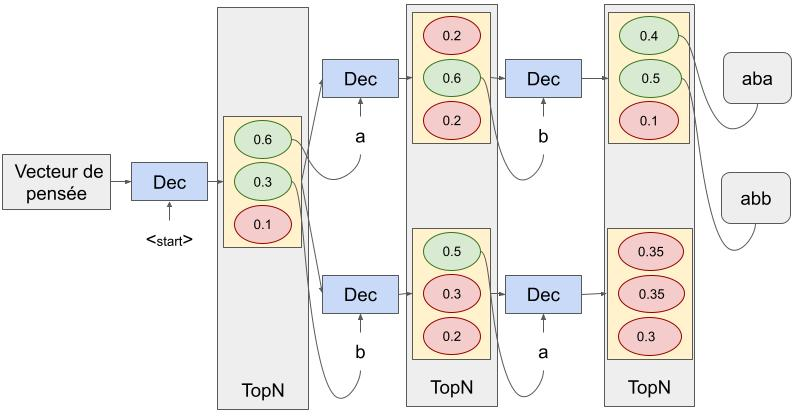
\includegraphics[scale=0.4]{2_production_mots_cles/Beam Search.jpg}
    \caption{Représentation schématique du processus de décodage grâce à l'algorithme de recherche en faisceau.}
    \label{fig:beam_search}
\end{figure}
\todo{refaire en tikz}

\`A l'inverse des algorithmes déterministes que nous avons décrits, notons l'existence des algorithmes d'échantillonnage. Ces algorithmes stochastiques choisissent les mots au hasard en fonction de leur probabilité. Les mots-clés générés par ces algorithmes ne sont donc pas reproductibles, ce qui dans le cadre de la production de mot-clés n'est pas souhaitable. Nous ne considérons donc pas cette technique.

\subsection{Paradigme encodeur-décodeur}\label{sub:paradigme_encodeur_decodeur}

Nous avons présenté dans les sections~\ref{sub:encoding} et \ref{sub:decoding} des moyens d'encoder des documents ainsi que des moyens de générer des séquences.
De nombreuses applications du traitement automatique de la langue nécessitent à la fois l'encodage d'une séquence et son décodage.
Par exemple dans le cadre de la traduction automatique, étant donnée une phrase en langue source, il faut la traduire dans une langue cible, c'est-à-dire qu'il faut encoder la phrase dans la langue source puis générer une phrase correspondante dans la langue cible.
Dans le cadre de la production de mots-clés, il faut générer un mot-clé en fonction d'un document.
Ainsi, le paradigme encodeur-décodeur introduit par \citet{sutskever_sequence_2014}, qui concatène un encodeur et un décodeur, permet de prendre en entrée une séquence de mots de longueur variable et de générer en sortie une autre séquence de mots de longueur variable.
Ce paradigme pallie la limite des réseaux de neurones présentés dans la section~\ref{sub:neural_network} (perceptrons mono ou multicouches) dont l'entrée et la sortie sont de taille fixe.

%Une fois une séquence encodée il est possible de la décoder, c'est-à-dire de produire un mot en fonction d'une représentation $h^t$.
%Générer un mot à partir d'une représentation $h_t$ consiste à passer la représentation dans un perceptron qui calcule une distribution de probabilité sur un vocabulaire, le mot à générer est choisis en fonction de sa probabilité.
    
%\begin{align}
    %\text{log}\: p(y|x) = \sum^m_{j=1} \text{log}\: p(y_j|y_{<j}, x)
%\end{align}

% FROM RECITAL SOTA

\colorlet{enccolor}{green!5}
\colorlet{inputcolor}{black!90!green}
\colorlet{deccolor}{blue!5}
\colorlet{outputcolor}{black!70!blue}
\colorlet{veccolor}{orange!15}
\colorlet{startendcolor}{black!60}
\colorlet{greybox}{black!3}

\begin{figure}[!htb]
\centering

\resizebox{\textwidth}{!}{%
\begin{tikzpicture}

\tikzstyle{cell}=[text centered, rectangle, draw, line width=.5pt, minimum height=1cm, minimum width=1.4cm, rounded corners=2pt]
\tikzstyle{word}=[font=\small\bfseries, text centered, minimum size=.5cm, minimum height=.3cm, text height=1.5ex, text depth=.25ex]
\tikzstyle{vector}=[text centered, rectangle, draw, line width=.5pt, minimum height=.5cm, minimum width=1cm, rounded corners=2pt]
\tikzstyle{arrow}=[shorten >= 2pt, shorten <= 2pt, draw=black!80]

\node[cell, fill=enccolor] (E1) at (0,0){};
\node[cell, fill=enccolor] (E2) at (2,0){};
\node[cell, fill=enccolor] (E3) at (4,0){};
\node[cell, fill=enccolor] (E4) at (6,0){};
\node[text centered] (E5) at (7.5,0){...};
\node[cell, fill=enccolor] (E6) at (9,0){};

\node[word, color=inputcolor, inner color=yellow!50, outer color=white] (I1) at (0,-1.2){Espace};
\node[word, color=inputcolor, inner color=yellow!50, outer color=white] (I2) at (2,-1.2){:};
\node[word, color=inputcolor, inner color=yellow!50, outer color=white] (I3) at (4,-1.2){la};
\node[word, color=inputcolor, inner color=yellow!50, outer color=white] (I4) at (6,-1.2){station};
%\node[word, color=inputcolor, inner color=yellow!50, outer color=white] (I5) at (8,-1.2){...};
\node[word, color=startendcolor] (I6) at (9,-1.2){<fin>};

%\node[cell, fill=veccolor, word, rotate=90] (V) at (11,0){vecteur de pensée};

\node[cell, fill=deccolor] (D1) at (11,0){};
\node[cell, fill=deccolor] (D2) at (13,0){};
\node[cell, fill=deccolor] (D3) at (15,0){};
%\node[cell, fill=deccolor] (D4) at (20,0){};

\node[word, color=startendcolor] (I7) at (11,-1.2){<début>};
\node[word, color=outputcolor, inner color=yellow!50, outer color=white] (O1) at (11,1.2){station};
\node[word, color=outputcolor, inner color=yellow!50, outer color=white] (O2) at (13,1.2){spatiale};
\node[word, color=startendcolor] (O3) at (15,1.2){<fin>};

\draw[->,>=latex,arrow] (E1) -- (E2) node[above,midway] {$h^e_0$};
\draw[->,>=latex,arrow] (E2) -- (E3) node[above,midway] {$h^e_1$};
\draw[->,>=latex,arrow] (E3) -- (E4) node[above,midway] {$h^e_2$};
\draw[->,>=latex,arrow] (E4) -- (E5) node[above,midway] {$h^e_3$};
%\draw[->,>=latex,arrow] (E5) -- (E6) node[above,midway] {$h^e_{n-1}$};
\draw[->,>=latex,arrow] (E5) -- (E6) node[above,midway] {$h^e_{n-1}$};

\draw[->,>=latex,arrow,shorten <= -2pt] (I1) to (E1);
\draw[->,>=latex,arrow,shorten <= -2pt] (I2) to (E2);
\draw[->,>=latex,arrow,shorten <= -2pt] (I3) to (E3);
\draw[->,>=latex,arrow,shorten <= -2pt] (I4) to (E4);
%\draw[->,>=latex,arrow,shorten <= -2pt] (I5) to (E5);
\draw[->,>=latex,arrow,shorten <= -2pt] (I6) to (E6);
\draw[->,>=latex,arrow,shorten <= -2pt] (I7) to (D1);


\draw[->,>=latex, arrow] (E6) -- (D1) node[above,midway] {$h^e_n$};

\draw[->,>=latex,arrow] (D1) -- (D2) node[above,midway] {$h^d_0$};
\draw[->,>=latex,arrow] (D2) -- (D3) node[above,midway] {$h^d_1$};
%\draw[->,>=latex,arrow] (D3) to (D4);

\draw[->,>=latex,arrow,shorten >= -2pt] (D1) to (O1);
\draw[->,>=latex,arrow,shorten >= -2pt] (D2) to (O2);
\draw[->,>=latex,arrow,shorten >= -2pt] (D3) to (O3);
%\draw[->,>=latex,arrow,shorten >= -2pt] (D4) to (O4);

%\node at (5,2) {\large{\textsc{Encodeur}}};
%\node at (17,2) {\large{\textsc{Décodeur}}};

\draw[arrow, rounded corners=3pt] (O1) -| (12, 0);
\draw[->,>=latex, arrow, rounded corners=3pt] (12, 0) -- (12, -1) -| (D2.south);

\draw[arrow, rounded corners=3pt] (O2) -| (14, 0);
\draw[->,>=latex, arrow, rounded corners=3pt] (14, 0) -- (14, -1) -| (D3.south);

%\draw[arrow, rounded corners=3pt] (O3) -| (19, 0);
%\draw[->,>=latex, arrow, rounded corners=3pt] (19, 0) -- (19, -1) -| (D4.south);

\draw[decoration={brace},decorate] (-0.7,1.7) -- node[below=-1.9em] {\large{\textsc{Encodeur}}} (9.7,1.7);
\draw[decoration={brace},decorate] (10.3,1.7) -- node[below=-1.9em] {\large{\textsc{Décodeur}}} (15.7,1.7);


\end{tikzpicture}
}

\caption{Exemple de modèle \textit{encodeur-décodeur} récurrent appliqué à l'extraction automatique de mots-clés.}
\label{fig:seq2seq}
\end{figure}


Le processus d'encodage et de décodage est décrit par l'équation~\ref{eq:enc-dec} et la figure~\ref{fig:seq2seq}.
Dans un premier temps la séquence d'entrée $X$ de taille $n$ est encodée dans le vecteur de pensée $h^e_n$.
Ce vecteur $h^e_n$ est utilisé pour initialiser le premier état caché du décodeur $h^d_0$.
Le décodeur génère ensuite les mots $\hat{y}_t$ qui composent la séquence de sortie $\hat{Y}$ à partir de cet état caché.

\begin{equation}\label{eq:enc-dec}
  \begin{split}
    p(\hat{y}_t | y_{1,...,t-1},h_0) & = \textsc{Softmax}(\sigma(b_v + W_v * h^d_t)) \\
    h^d_t & = \textsc{Rnn}^d(\hat{y}_{t-1}, h^d_{t-1}) \\
    \hat{y}_0 & = \textsc{Debut} \\
    h^d_0 & = h^e_n \\
    h^e_n & = \textsc{Rnn}^e(X) \\
  \end{split}
\end{equation}

Nous présentons ci-après deux améliorations de ce paradigme.
%
D'abord, le mécanisme d'attention qui permet de porter attention à une partie spécifique de l'entrée lors du décodage. Par exemple, la description d'une image nécessite d'identifier les différents objets qui la composent.
%
Ensuite, le mécanisme de copie qui pallie l'incomplétude du vocabulaire de sortie. Ce mécanisme permet au décodeur de copier un mot du document d'entrée au lieu de le générer à partir du vocabulaire de sortie. Le mécanisme de copie est particulièrement utile pour les entités nommées par exemple. Ces entités sont peu fréquentes et ne font généralement pas partie du vocabulaire de sortie.

% Convolution
%Les réseaux de neurones à convolution sont surtout utilisés pour le traitement d'images. Dans le cas du texte, des 
    
% Graphes
%Les réseaux à convolution de graphes (GCN) permettent d'obtenir pour chaque noeud d'un graphe un embedding en fonction de ses voisins. Le nombre de convolutions représente le nombre de bonds qui sont fait entre les noeuds.
    
% Transformer
%Les transformer ont été introduit par \cite{vaswani_attention_2017} et utilisent un mécanisme de self-attention pour chaque mot d'une séquence, de sorte à obtenir pour chaque mot un vecteur qui représente sa relation avec chaque autre mot. Ce mécanisme ne prend pas en compte la séquentialité, en effet chaque calcul est parallélisable. Et ce modèle qui requiert une force de calcul colossale a montré de très bons résultats sur de nombreuse tâches.

\subsubsection{Mécanisme d'attention}
\label{sub:attention_mecanism}

Le mécanisme d'attention~\cite{bahdanau_neural_2014,luong_effective_2015} a été introduit pour améliorer le traitement de longues séquences en permettant au modèle de se focaliser sur certaines parties du document lors du décodage.
%
En effet, un mot-clé concerne seulement certains aspects d'un document. Ce mécanisme permet donc au modèle de porter attention aux parties du document liées à ces aspects.
%
De plus, cette attention au document peut être visualisée grâce aux \emph{poids d'attention} calculés à chaque étape de décodage.
%Par exemple, dans le cadre de la traduction automatique, il permet de visualiser l'alignement entre la phrase en langue source et la phrase en langue cible.
%Par exemple, dans le cadre de la traduction automatique, ce mécanisme permet de visualiser l'importance de chaque mot du document source pour générer la traduction.
La figure~\ref{fig:attention_alignment} illustre cette attention dans le cadre de la traduction automatique pour traduire en français la phrase \say{The agreement on the European Economic Area was signed in August 1992.}
%Il existe généralement un alignement monotone entre les phrases en français et les phrases en anglais.
%Mais ce n'est pas toujours le cas comme le montre le syntagne nominal \say{European Economic Area} dont les mots de la traduction sont dans un ordre inverse \say{zone économique européenne}.
%Le modèle a pu, grâce au mécanisme d'attention, proposer la bonne traduction \say{zone économique européenne} dont l'ordre des mots est inverse à sa traduction.
% Même si le français et l'anglais peuvent généralemnt être traduit mot à mot de manière monotone, le mécanisme d'attention nous permet de visualiser l'alignement non monotone entre zone économique européenne et European Economic Area, en effet l'ordre des noms et adjectifs en français et en anglais est différent.
%Ainsi nous pouvons observer que pour traduire \say{was} en \say{a été}, le modèle à porté attention à \say{was signed} pour comprendre que \say{was} fait parti de la construction du prétérit.
%Pour illustrer ce mécanisme dans le cadre de la traduction automatique nous prenons l'exemple suivant: pour traduire la séquence \say{the European Economic Area} en français (\say{\foreign{la zone économique européenne}}) le modèle portera attention à chaque mot du texte source. Ainsi, pour générer \say{la} et \say{zone} il devra porter attention à \say{\foreign{the}} et \say{\foreign{Area}}. \todo{A revoir.}

\begin{figure}
    \centering
    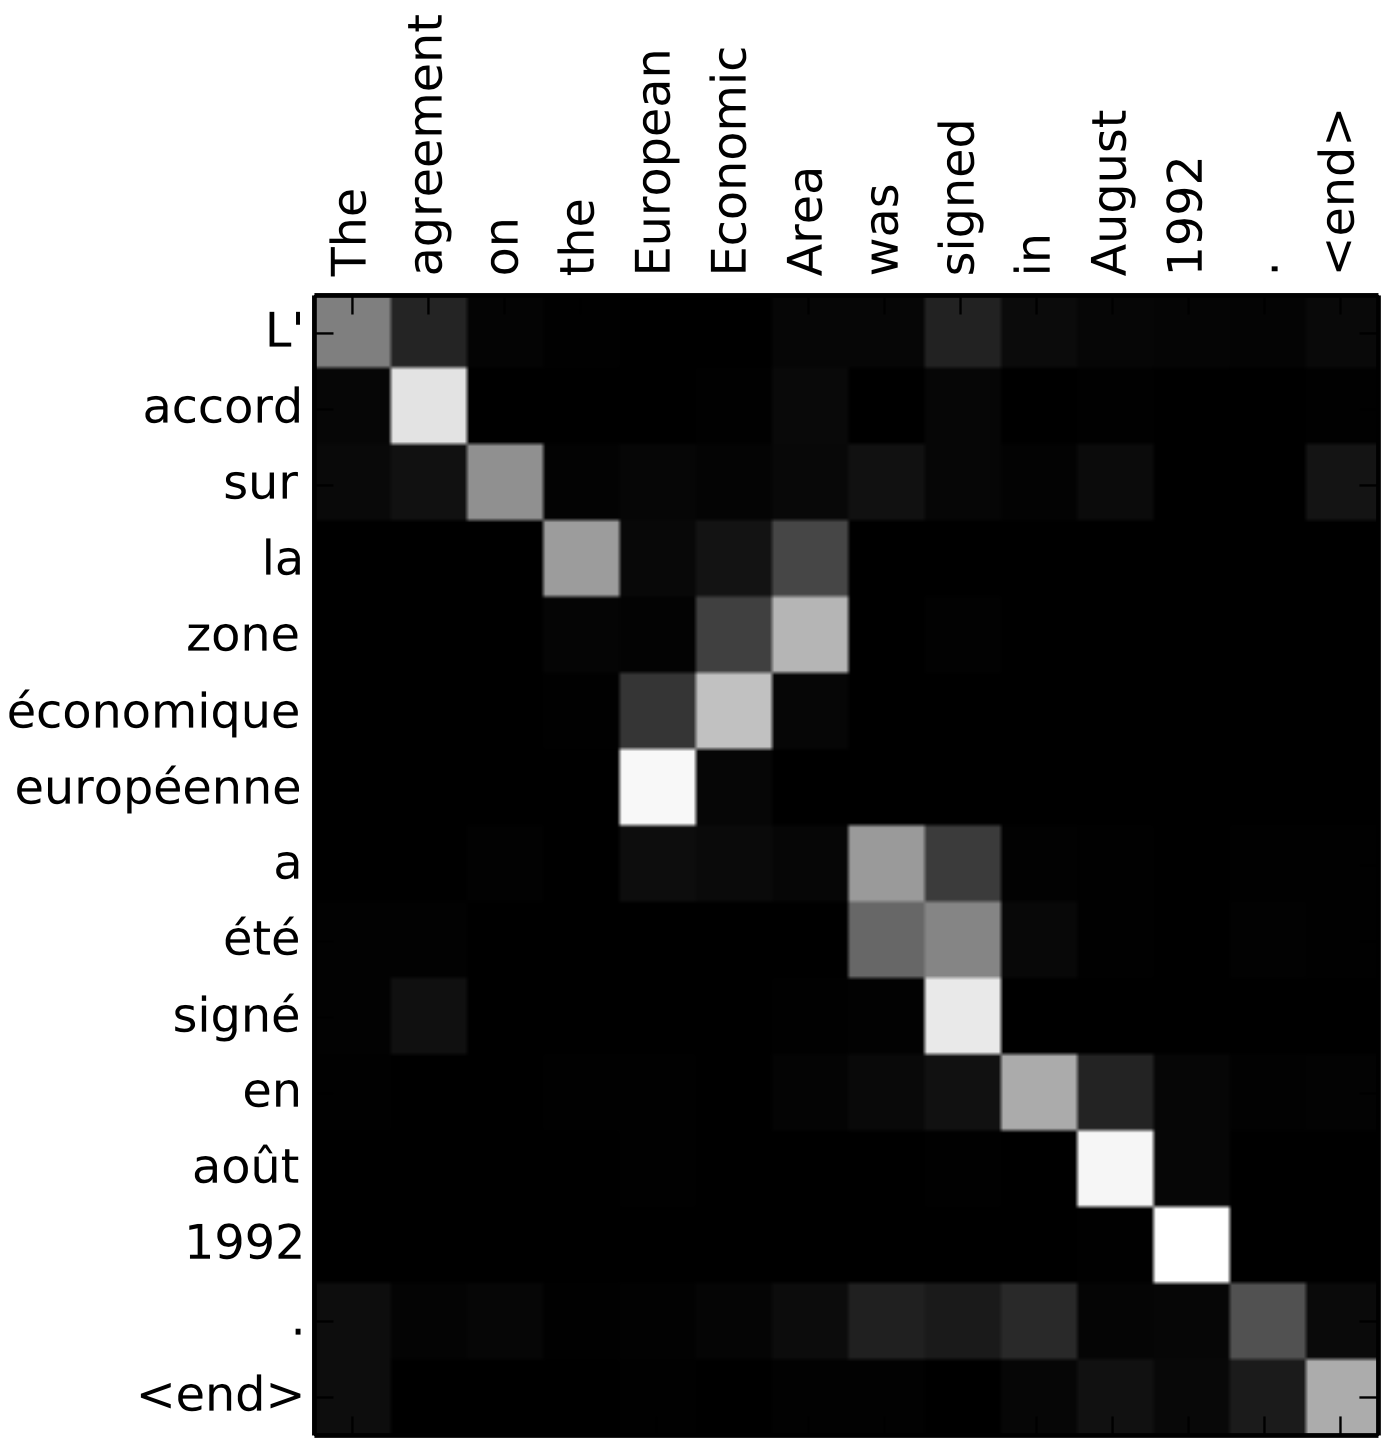
\includegraphics[scale=0.3]{2_production_mots_cles/attention_alignment.png}
    \caption{Exemple de visualisation des poids d'alignement du mécanisme d'attention entre une phrase en anglais et sa traduction en français. Chaque ligne montre la distribution des poids $\alpha_{t}$ ayant servis à générer le mot correspondant en français. Une case blanche indique un poids de 1, une case noire indique un poids de 0. Image extraite de \citet{bahdanau_neural_2014}.}
    \label{fig:attention_alignment}
\end{figure}

%Il faudra aussi porter attention à la syntaxe des deux langues
%Les poids d'attention peuvent être utilisés pour visualiser l'alignement entre les mots de la séquence d'entrée et ceux de la séquence de sortie.
%La figure~\ref{fig:attention_alignment} montre les poids d'alignement dans le cadre de la traduction automatique entre une phrase en anglais et sa traduction en français.

Le décodeur utilise l'état caché courant $h^d_t$ pour générer un mot, le mécanisme d'attention lui permet d'utiliser aussi tous les états cachés de l'encodeur $h^e$ pour mettre à jour l'état caché du décodeur $h^d_t$. Ce mécanisme est décrit dans l'équation~\ref{eq:attention}.
Dans le mécanisme d'attention, les états cachés $h^e$ sont pondérés en fonction de leur importance pour générer le mot $\hat{y}_t$.
Cette importance est établie grâce à une fonction d'alignement $a$ qui calcule une similarité entre l'état caché courant $h^d_t$ et ceux de l'encodeur $h^e$.
Les états cachés $h^e$ sont ainsi moyennés dans le vecteur de contexte $c_t$ utilisé pour mettre à jour l'état caché courant du décodeur $h^d_t$.

Dans l'équation \ref{eq:attention}: $[u;v]$ représente l'opération de concaténation des vecteurs $u$ et $v$; $a$ est une fonction d'alignement qui calcule la similarité entre un état caché de l'encodeur $h^e_t$ et du décodeur $h^d_t$; $\alpha$ représente les poids d'alignement entre les états cachés de l'encodeur $h^e$ et du décodeur $h^d$;  et $\textsc{Softmax}$ est une fonction qui normalise les valeurs d'un vecteur pour qu'il somme à 1.


\iffalse
    \begin{figure}
        \centering
        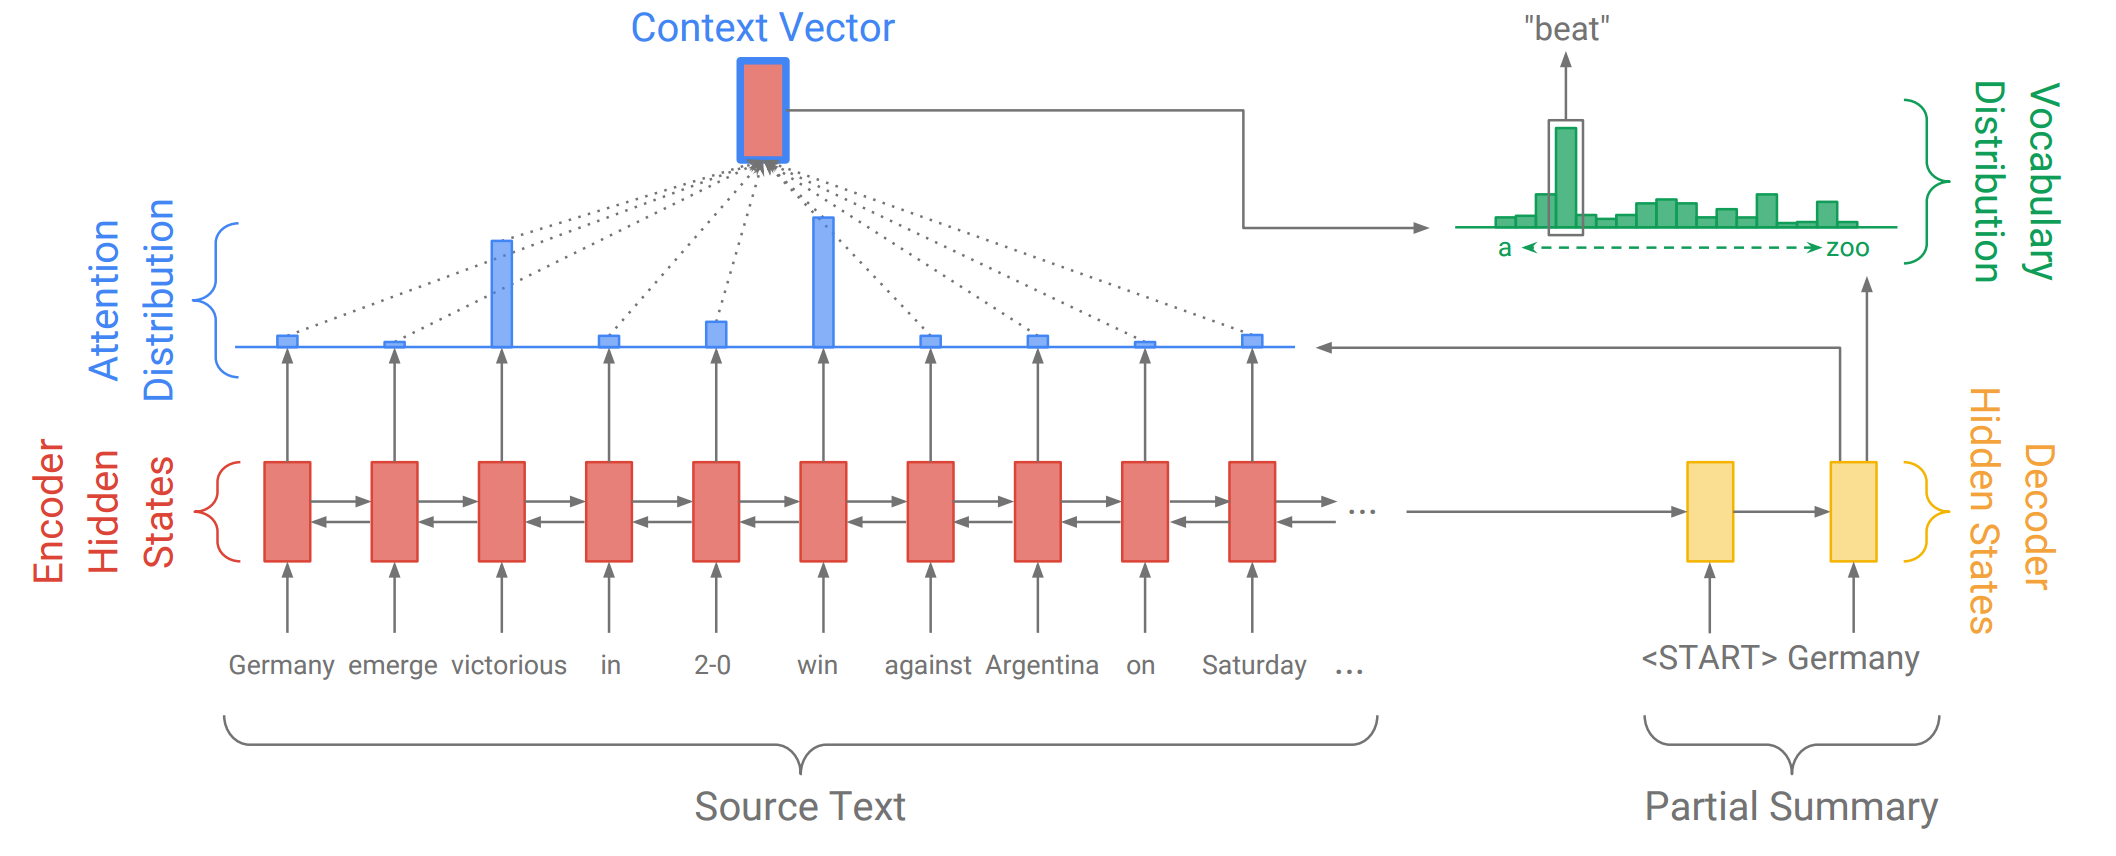
\includegraphics[width=\linewidth]{figures/see_seq2seq-attn.png}
        \caption{Schéma du mécanisme de copie présenté par \cite{see_get_2017}.}
        \label{fig:see_attention}
    \end{figure}
\fi

\begin{equation}\label{eq:attention}
  \begin{split}
    %\hat{Y}_t & = \sigma(b_v + W_v * h^d_t) \\
    p(y_t|y_{<t},x) & = \textsc{Softmax}(\sigma(W_v h^d_t)) \\[.3em]
    h^d_t & = \textsc{Rnn}(y_{t-1}, [h^d_{t-1};c_t]  \\[.3em]
    c_t & = \sum^{|h^e|}_{i=0} \alpha_{i,t} h^e_i \\
    \alpha_{t} & = \textsc{Softmax}(a(h^d_t, h^e)) \\
    %\textsc{Softmax}(x) & = \left[ \frac{x_i}{\sum^{|x|}_{i=0} x_i} , i \in |x| \right]
  \end{split}
\end{equation}

%Le concept d'attention a été présenté de deux manières différentes par \cite{bahdanau_neural_2014} et \cite{luong_effective_2015}.
%
%L'idée de l'attention présentée par~\cite{luong_effective_2015} est \emph{d'utiliser le vecteur de contexte pour prédire $y_t$}.
%
%\cite{bahdanau_neural_2014} présente un autre mécanisme d'attention dont l'idée est de calculer l'état caché du décodeur à l'aide d'un vecteur de contexte. Par rapport à un décodeur classique, seul le calcul de $h^d_t$ change.

\iffalse
    L'idée de l'attention présentée par~\cite{luong_effective_2015} est \emph{d'utiliser le vecteur de contexte pour prédire $y_t$}.
    
    Pour cela, un nouveau $\hat{h}^d_t$ est calculé en fonction d'un vecteur de contexte $c_t$ et de $h^d_t$ (calculé en fonction de $y_{t-1}$ et $h^d_{t-1}$). $c_t$ est la moyenne des $h^e$ pondérés par les scores d'alignement $\alpha$.
    
    Dans leur article, deux manières de calculer l'attention sont présentées: une attention globale et une attention locale.
    %
    Pour l'attention globale, le vecteur de contexte est la moyenne pondérée de toutes les représentations de l'encodeur.
    %
    Pour l'attention locale, le vecteur de contexte est la moyenne pondérée des représentations $h^e$ dans une fenêtre de taille $D$ autour de $h^e_{p_t}$.
    %
    $p_t$ est une valeur entre 0 et $|h^e|$ qui définit le centre de la fenêtre, et peut être calculé de différentes manières.\footnote{Pour plus de détails voir la section 3.2 de \cite{luong_effective_2015}}
    %$p_t$ étant $t$ (dans la traduction automatique on considère que le mot cible $y_t$ est aligné avec le mot source $x_{p_t}$), ou alors un réel entre 0 et $|h^e|$ calculé à l'aide 
    
    \begin{align}
        %y_t & = \sigma(W_v h^d_t) \\
        p(y_t | y_{<t}, x) & = \textsc{Softmax}(W_v \hat{h}^d_t) \\
        \hat{h}^d_t & = \sigma(W_c [c_t;h^d_t]) \\
        c_t & = \sum^{|h^e|}_{i=0} \alpha_{i,t} * h^e_i \\
        \alpha_{i,t} & = \textsc{Softmax}(a(h^e_i, h^d_t)) \\
        h^d_t & = \textsc{Rnn}(y_{t-1}, h^d_{t-1})
    \end{align}
    
    \cite{bahdanau_neural_2014} présente un autre mécanisme d'attention dont l'idée est de calculer l'état caché du décodeur à l'aide d'un vecteur de contexte. Par rapport à un décodeur classique, seul le calcul de $h^d_t$ change. Le calcul du vecteur de contexte est similaire à celui de ~\cite{luong_effective_2015}.
    
    \begin{align}
        p(y_t|y_{<t},x) & = \textsc{Softmax}(W_v h^d_t) \\
        h^d_t & = \textsc{Rnn}(y_{t-1}, [h^d_{t-1};c_t]  \\
        c_t & = \sum^{|h^e|}_{i=0} \alpha_{i,t} * h^e_i \\
        \alpha_{i,t} & = \textsc{Softmax}(a(h^e_i, h^d_t))
    \end{align}
    
    Il existe différentes fonctions d'alignement:
    
    bahdanau $a(h^e_i, h^d_t) = v_a \text{tanh}(W_a h^d_t + U_a h^e_i)$
    
    dot $a(h^e_i, h^d_t) = h^e_i h^d_t$
    
    general $a(h^e_i, h^d_t) = h^e_i W_a h^d_t$
    
    concat $a(h^e_i, h^d_t) = W_a [h^e_i;h^d_t]$
\fi

\subsubsection{Mécanisme de copie}
\label{sub:copy_mecanism}

Le mécanisme de copie~\cite{see_get_2017,gu_incorporating_2016} provient des tâches de traduction automatique et de résumé automatique. Il a pour but de produire des mots peu fréquents ou hors du vocabulaire de sortie.
En effet, les modèles neuronaux qui génèrent du texte choisissent les mots dans un vocabulaire de sortie comportant généralement \num{50 000} mots.
Dans les tâches sus-citées, les mots peu fréquents qui ne font pas partie du vocabulaire de sortie, comme les entités nommées ou les transfuges, doivent pourtant apparaître dans la séquence de sortie.
%Le mécanisme de copie ~\cite{see_get_2017,gu_incorporating_2016} pallie ce problème en permettant au décodeur de générer un mot du vocabulaire de sortie ou bien de copier un mot du document.
Deux mécanismes de copie ont été proposés par \citet{see_get_2017} et \citet{gu_incorporating_2016}; les deux étant similaires, nous présentons ici le premier car plus simple. Il est décrit dans l'équation~\ref{eq:copy_mecanism}.

% exemple
%Le mécanisme d'attention a été utilisé comme post-traitement pour remplacer les mots inconnus de la sortie par les mots de l'entrée alignés par le mécanisme d'attention. Ceci permettant de traiter les entités nommées peu fréquentes ou les transfuges.
%
%Le mécanisme de copie vient automatiser ce processus en permettant au modèle de générer un mot du vocabulaire ou de copier un mot du document.

%, tous deux inspirés des réseaux de pointeurs~\cite{vinyals_pointer_2015} qui génèrent une séquence de pointeurs vers la séquence d'entrée.
Ce mécanisme utilise le vocabulaire de la séquence d'entrée $\mathcal{X}$ (particulier à chaque document) en plus du vocabulaire de sortie $\mathcal{V}$.
Pour produire un mot, une distribution de probabilité sur le vocabulaire  $P_{vocab}(y_{t})$ est calculée comme précédemment par le décodeur (cf. section~\ref{sub:decoding}) et les poids du mécanisme d'attention $\alpha$ (cf. section~\ref{sub:attention_mecanism}) sont utilisés pour estimer la probabilité de copie de chaque mot du document.
Les poids d'attention $\alpha$ des mots qui apparaissent plusieurs fois dans l'entrée $x$ sont sommés $\sum_{j,x_j=y_{t,i}} \alpha^t_j$.
Ainsi, un mot peut être généré à partir du vocabulaire de sortie $\mathcal{V}$ ou copié à partir du vocabulaire du document $\mathcal{X}$.
Les probabilités de copie et de génération d'un même mot, qui appartient au document et au vocabulaire, sont sommées.
Dans l'équation~\ref{eq:copy_mecanism}: $h^d_t$, $c_t$ et $\alpha^t_j$ proviennent du mécanisme d'attention (cf. équation~\ref{eq:attention}); $p_{gen}$ est un curseur permettant au modèle de privilégier la copie ou la génération et $P_{vocab}(y_t)$ est une distribution de probabilité sur le vocabulaire de sortie $\mathcal{V}$.

%Les probabilités de génération et de copie sont combinés pour donner une distribution de probabilités sur $\mathcal{X} \cup \mathcal{V}$.

\begin{equation}\label{eq:copy_mecanism}
  \begin{split}
    p(y_{t,i}|y_{<t},x) & = p_{gen} P_{vocab}(y_{t,i}) + (1 - p_{gen}) \sum_{j,x_j=y_{t,i}} \alpha^t_j \\
    p_{gen} & = \sigma(W_h h^d_t + W_c c_t + W_y y_{t-1}) \\
    P_{vocab}(y_{t}) & = \textsc{Softmax}(\sigma(W_v h^d_t))
  \end{split}
\end{equation}

%ou les poids d'un mécanisme d'attention supplémentaire, utilisé seulement pour calculer le score de copie, pour~\cite{gu_incorporating_2016}

\iffalse
    %\cite{gu_incorporating_2016}, création d'un vocabulaire spécifique a chaque instance, composé de $\mathcal{V}$ le vocabulaire normal et $\mathcal{X}$ le vocabulaire des mots de l'entrée.
    %
    %Ça change le calcul de $y_t$ par rapport au mécanisme d'attention.
    %
    %On défini les vecteurs $\psi_g \in \mathds{R}^|\mathcal{V}|$ et $\psi_c \in \mathds{R}^|\mathcal{X}|$ qui contiennent respectivement les score de copie et de génération.
    
    % attentive read = les poids de l'attention
    % selective read = les poids de l'"attention" du mécanisme de copie
    
    \begin{align}
        y_t & = \textsc{Softmax}(e^{P_{gen}} +e^{P_{copy}}) \\
        P_{gen} & = W_v h^d_t \\
        P_{copy} & = \left[ \sum^{|h^e|}_{j=0, x_j=x_i} \sigma(h^e_j W_c) h^d_t | x_i \in \mathcal{X} \right] \\
        h^d_t & = RNN([y_{t-1};cc_t)],h^d_{t-1}) \\
        cc_t & = \sum^{|h^e|}_{i=1} aa_{t,i} h^e_t \\
        aa_{t,i} & = \textsc{Softmax}()
    \end{align}
    
    %\cite{see_get_2017} reprend le mécanisme d'attention de \cite{luong_effective_2015} et modifie le calcul de $y_t$ en ajoutant une probabilité de copie et un curseur privilégiant la copie ou la génération.
    
    \begin{align}
        p(y_{t,i}) = p_{gen} P_{vocab}(y_{t,i}) + (1 - p_{gen}) \sum_{j,x_j=y_{t,i}} \alpha^t_j \\
        p_{gen} = \sigma(W_c c_t + W_h h^d_t + W_y y_{t-1})
    \end{align}
\fi

% Multitache
% Conditional Random Field
% Reinforcement Learning : adaptative reward


\section{Méthodes de bout-en-bout}
\label{methodes-de-bout-en-bout}

\todo{Ajouter des schéma pour mieux comprendre les méthodes.}

Dans cette section nous présentons un état de l'art des méthodes de bout-en-bout.
Ces méthodes, contrairement aux méthodes en chaîne de traitement (cf. section~\ref{sec:methode-en-chaine-de-traitement}), prennent en entrée un document et laissent le soin au modèle d'en extraire les caractéristiques pour retourner un ensemble de mots-clés sans étapes intermédiaires ni définition manuelle de ces caractéristiques.
Parmi les méthodes proposées dans la littérature, nous distinguons les méthodes génératives, qui peuvent produire des mots-clés présents et des mots-clés absents, des méthodes extractives, limitées aux mots-clés présents.

Jusqu'à présent, toutes les méthodes de bout-en-bout qui ont été proposées sont supervisées et reposent sur des réseaux de neurones (cf. section~\ref{sub:neural_network}) qui nécessitent de grandes quantités de données annotées pour être entraînées.
%
Le développement de ces méthodes démarre avec l'introduction du jeu de données KP20k et de la méthode générative CopyRNN par \citet{meng_deep_2017}.
Le jeu de données KP20k, qui comporte $\simeq$\num{550000} documents, comble un manque.
En effet, seuls de petits jeux de données (de l'ordre du millier de documents) étaient jusqu'alors disponibles.
Ce travail a ainsi lancé une nouvelle direction de recherche sur les méthodes génératives de production de mot-clés.

\begin{figure}
    \centering
    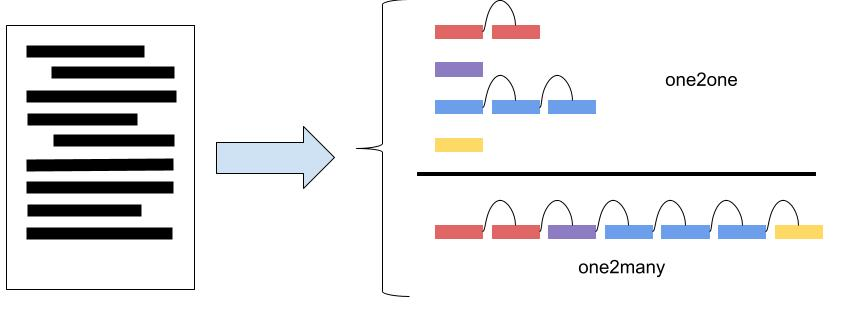
\includegraphics[scale=0.4]{2_production_mots_cles/Decoding strategies.jpg}
    \caption{Représentation schématique des stratégies de décodage \emph{one2one} et \emph{one2many}.}
    \label{fig:decoding_strategies}
\end{figure}
\todo{Refaire en tikz}

Dans cet état de l'art, nous présentons tout d'abord les méthodes automatiques de génération de mots-clés de bout-en-bout, qui sont au c\oe{}ur de ce travail de thèse.
Nous présentons ces méthodes de génération en deux parties: premièrement, les méthodes qui générent les mots-clés un à un (\emph{one2one}), et deuxièmement, celles qui génèrent des séquences de mots-clés (\emph{one2many}). Ces deux types de génération sont schématisés dans la figure~\ref{fig:decoding_strategies}.
Nous présentons ensuite les méthodes extractives de bout-en-bout, c'est-à-dire celles qui se limitent aux seuls mots-clés présents.

\subsection{Génération de mots-clés}
\label{sub:generation_de_mots_cles}

Les méthodes génératives, introduites par \citet{meng_deep_2017}, ont pour objectif de pallier deux faiblesses qui concernent la majorité des méthodes extractives présentées précédemment: l'impossibilité de produire des mots-clés absents ainsi que la faible prise en compte de la sémantique.
Le paradigme encodeur-décodeur sur lequel les méthodes génératives sont fondées permet d'encoder la sémantique du document.
Ainsi, les mots-clés produits sont le fruit d'une \say{compréhension} du document, contrairement aux méthodes en chaîne de traitement qui s'intéressent à l'\say{importance} des mots dans le document indépendamment de leur sens.
%
Ces méthodes génératives rendent possible la production de mots-clés absents grâce à la manière dont le décodeur génère la séquence de sortie.
Ce processus s'effectue en choisissant, à chaque étape de décodage, un mot à partir d'un vocabulaire de sortie qui est plus grand et différent du vocabulaire du document.
Ces méthodes génératives apprennent à générer des mots-clés un par un (génération \emph{one2one}, voir figure~\ref{fig:decoding_strategies}), c'est-à-dire que chaque document $X$ et son ensemble de mot-clés $Y$ de taille $N$ forment un couple $(X, \{Y_0, ..., Y_N\})$, décomposé en autant d'exemples d'entraînement que de mots-clés, $(X, Y_0), ... , (X, Y_N)$.

%\paragraph{Définitions}
%\todo{Il faudrait définir avant les principaux modèles: one2one, séquence avant de les définir formellement; Fait ausi des dessins}
%$x$ et $y$ représentent des mots, $p$ des mots-clés. Étant donné un ensemble de données $D = {(x^i,p^i), i \in 1...N}$ de taille $N$, un exemple est composé d'un document $x^i$ et d'un ensemble de mots-clés $p^i = {p^i_j, j \in 1...M^i}$ de taille $M^i$. Les documents et les mots-clés sont composés de mots $[x^i_k, k \in 1...N^i]$ et $[y^i_j]$ est composé d'un document composé d'une séquence de mots $x^i = (x^i_1, ..., x^i_{N^i})$ de longueur $N^i$ et d'un ensemble de mots-clés $p^i$ de taille $M^i$ avec $p^i = (p^i_1, ..., p^i_{M^i})$, où chaque mot-clé est une séquence de mots de taille $M^{i,j}$ avec $p^{i,j} = (y^{i,j}_1, ..., y^{i,j}_{M^{i,j}})$. Dans le cadre des modèles one2one, un couple document -- mots-clés est découpé en $M^i$ différents couples $(x^i, p^{i,1}), ..., (x^i, p^{i, M^i})$. 
%Pour les modèles en séquences, les mots-clés sont concaténés de sorte à former une unique séquence $(x^i, y^{i,1}_1 \lozenge ... \lozenge y^{i,1}_{M^{i,j}} \lozenge \text{SEP} \lozenge y^{i,2}_1 \lozenge ... \lozenge y^{i,M^i}_{M^{i,j}})$.

La méthode pionnière de génération automatique de mots-clés appliquée aux documents scientifiques est CopyRNN~\cite{meng_deep_2017}.
%
L'architecture neuronale de cette méthode s'inspire du processus d'annotation humain qui consiste à lire le document pour le comprendre dans son entièreté puis à le résumer grâce à des mots-clés.
%Aussi, les humains peuvent facilement s'abstraire du texte et faire appel à leurs connaissances pour produire des mots-clés qui n'apparaissent pas dans le texte.
Pour reproduire ce processus, CopyRNN utilise le paradigme encodeur-décodeur, que nous avons présenté dans la section~\ref{sub:paradigme_encodeur_decodeur}, pour encoder un document et le décoder ensuite en un mot-clé. % Ainsi un réseau de neurones récurrent encode le document dans un vecteur de pensée, puis un autre décode, génère, ce vecteur de pensée en un mot-clé.
Pour améliorer les performances des modèles encodeur-décodeur, il est commun d'utiliser un mécanisme d'attention (voir section~\ref{sub:attention_mecanism}).
Ce mécanisme permet au modèle de porter attention à certaines parties du document lors de la génération d'un mot.
%
Un mécanisme de copie est aussi ajouté au modèle pour lui permettre de générer des mots peu fréquents (voir section~\ref{sub:copy_mecanism}).
Ce mécanisme de copie modifie le décodage en permettant de générer un mot à partir du vocabulaire de sortie ou bien à partir du document.\\
%
Cette méthode obtient des performances bien plus élevées que les précédentes méthodes extractives. Les performances de CopyRNN sont de l'ordre de 30 points de \fmesure{} pour les mots-clés présents tandis que les performances des méthodes extractives sont généralement en dessous de 20 points de \fmesure{}.
Les mots-clés absents, qui ne pouvaient jusque-là pas être produits, correspondent peu à la référence: parmi les 50 meilleurs mots-clés absents un seul apparaît dans la référence.


%La communauté scientifique présente de nouvelles méthodes basées sur CopyRNN et tente de l'améliorer.
% les méthodes essaient de résoudre les problèmes identifiés
%Les méthodes présentées augmentent toujours les performances de génération des mots-clés présents et absents.

Certaines méthodes proposées essaient d'améliorer l'encodage du document.
\citet{chen_title-guided_2019}, par exemple, constate que les mots-clés ne sont pas uniformément distribués dans les documents.
En particulier \npercent{60} des mots-clés de référence ont au moins un mot en commun avec le titre du document.
Pour prendre cela en compte, ils proposent TGNet (Title Guided Network), qui étend CopyRNN en introduisant un nouvel encodeur spécifique au titre, en plus de l'encodeur du document.
Cet encodage du titre permet de donner un poids supplémentaire à l'information qu'il contient.
Ces deux représentations (du titre et du document) sont ensuite combinées puis fournies au décodeur.
Cette méthode améliore nettement les performances de génération des mots-clés présents et absents par rapport à CopyRNN (+\npercent{5} sur KP20k).
% Ils ne regardent que la F-mesure présent/absent rien d'autre

La redondance dans les ensembles de mots-clés produits est un problème récurrent dans les méthodes de production de mots-clés.
En effet, \citet{hasan_automatic_2014} montrent que 8 à \npercent{12} des erreurs des méthodes sont liées à la redondance des mots-clés.
Ainsi, les méthodes en chaîne de traitement mettent en place des stratégies, notamment lors de la sélection du sous-ensemble de mots-clés, pour limiter cette redondance (voir section~\ref{choisir-le-sous-ensemble}).
Dans cette ligne de recherche, \citet{zhao_incorporating_2019} remarquent les méthodes de bout-en-bout ne sont pas exemptes de ce problème, ils s'intéressent ainsi au chevauchement entre les mots-clés générés et ceux de référence.
Par exemple, \npercent{23.98} des mots-clés unigrammes générés par CopyRNN font partie d'un mot-clé de référence, et \npercent{47.15} des mots-clés 4-grammes générés par CopyRNN contiennent un mot-clé de référence.
Dans l'optique de limiter ces chevauchement, ils présentent le modèle ParaNet$_T$+CoAtt qui entraîne le modèle, à générer à la fois les mots-clés et leurs étiquettes morphosyntaxiques, ainsi la syntaxe des mots-clés générés sera similaire à celle des mots-clés de référence.
Pour cela ils ajoutent au modèle CopyRNN un encodeur, pour les étiquettes morphosyntaxiques des mots du document, ainsi qu'un décodeur, pour celles du mot-clé.\footnote{Les étiquettes morphosyntaxiques du document et des mots-clés proviennent de l'outils Stanford CoreNLP.}
Les informations des deux décodeurs sont ensuite combinées et utilisées pour générer les mots-clés et leurs étiquettes morphosyntaxiques.
%Grâce à cette méthode, les mots-clés générés chevauchent moins les mots-clés de référence; par exemple le pourcentage de mot-clés 4-grammes contenant un mot-clé de référence a baissé de \npercent{10}.

\begin{figure}
    \centering
    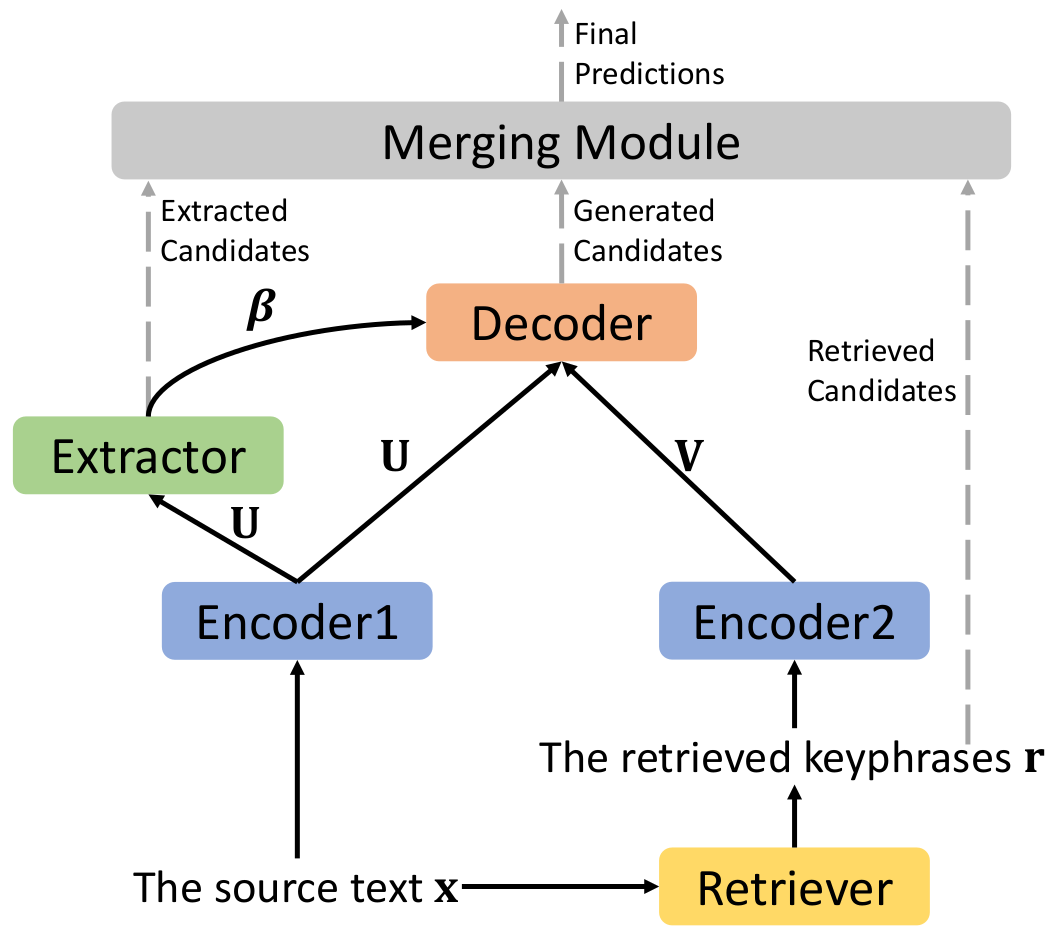
\includegraphics[scale=0.2]{2_production_mots_cles/kg_ke_kr_m.png}
    \caption{Représentation schématique de l'architecture de la méthode KG-KE-KR-M. Image extraite de~\citet{chen_integrated_2019}.}
    \label{fig:schema_kgkekrm}
\end{figure}

%Le processus manuel d'annotation en mots-clés est composé de plusieurs étapes: la lecture du document, l'extraction des mots-clés dans le document puis l'attribution de mots-clés absents du document et enfin la combinaison des mots-clés provenant de ces deux processus d'annotation.
Dans l'optique de reproduire l'annotation humaine, \citet{chen_integrated_2019} propose la méthode KG-KE-KR-M qui produit un ensemble de mots-clés en combinant différentes méthodes: génération de mots-clés, extraction de mots-clés, récupération de mots-clés (voir figure~\ref{fig:schema_kgkekrm}).
%Ces différentes méthodes sont entraînées de bout-en-bout puis les mots-clés de chaque méthode sont pondérés grâce à un classifieur.
%
Dans un premier temps, cette méthode récupère les mots-clés de référence des $K$ documents d'entraînement les plus proches du document traité (grâce à la distance de Jaccard).
Ces mots-clés \emph{récupérés} sont concaténés puis encodés. Ils serviront à conditionner la génération de mots-clés.
Dans un second temps, des mots-clés sont \emph{extraits} du document en classifiant chaque mot comme mot-clé ou non mot-clé.
%Cette classification s'effectue grâce aux états cachés du document encodé.
Ensuite, des mots-clés sont \emph{générés} à partir du document ainsi que des mots-clés récupérés et des mots-clés extraits.
Enfin, les mots-clés récupérés, extraits et générés sont pondérés grâce à un classifieur.
Cette méthode à la particularité de combiner les méthodes en chaîne de traitement (sélection de candidats puis pondération) et les méthodes de bout-en-bout (apprentissage conjoint de la génération et de l'extraction).
Malgré la grande diversité dans les techniques de production de mots-clés candidats, les performances ne sont pas significativement supérieures à CopyRNN. Cette méthode produit néanmoins plus de mots-clés absents de référence que CopyRNN.

La méthode CorrRNN~\cite{chen_keyphrase_2018} considère que les mots-clés doivent couvrir l'ensemble des sujets du document et être divers, c'est-à-dire que chaque mot-clé doit concerner un sujet différent.
Cette méthode étend CopyRNN en y ajoutant un mécanisme de couverture et un mécanisme de revue.
Le mécanisme de couverture encourage le modèle à porter attention aux différentes parties du document.
Il conserve et accumule les scores d'attention des mots du document à chaque étape de décodage, et il est inclus dans le calcul du mécanisme d'attention.
Ensuite, le mécanisme de revue est essentiellement un mécanisme d'attention sur les mots générés.
Son objectif est d'identifier les sujets déjà couverts par les mots-clés générés et ainsi de générer des mots-clés qui concernent des sujets non traités.
Cette méthode est la première à prendre en compte les mots-clés déjà générés dans le processus de génération, pour cela la phase d'entraînement est modifiée.
Au lieu de rétro-propager le gradient après chaque mot-clé de référence, la phase de rétro-propagation n'est effectuée qu'une fois tous les mots-clés de référence du document traités.
%Chaque mot-clé est généré en utilisant les mécanismes de couverture et de redondance, qui prennent en compte les mots-clés déjà générés; le gradient est ensuite calculé grâce à l'erreur de chaque mot-clé; et enfin, rétro-propagé.
%Cette méthode améliore les performance de production de mots-clés présent par rapport à CopyRNN, mais l'article ne présentant pas ses résultats sur le jeu de données de référence KP20k et utilisant des métriques peu utilisés dans les autres travaux la comparaison est limitée.

\subsection{Génération de séquences de mots-clés}% (\textsc{One2Seq})}
%\subsection{Génération en séquence}
\label{sub:generation_de_sequences_de_mots_cles}

%Nous avons présenté dans la section précédente, des méthodes génératives qui apprennent à générer un mot-clé par document.
Nous présentons dans cette section des méthodes qui apprennent à générer des séquences de mots-clés (génération \emph{one2many}, voir figure~\ref{fig:decoding_strategies}). C'est-à-dire que chaque exemple d'entraînement est composé d'un document et de la concaténation des mots-clés de référence en une unique séquence dans laquelle ils sont séparés par un symbole de séparation. Par exemple, l'ensemble de mots-clés $\{$ Classe , Fichier log , Agrégat $\}$ sera transformé en \say{Classe \texttt{SEP} Fichier log \texttt{SEP} Agrégat \texttt{FIN}}.
%Le développement des méthodes utilisant la génération \emph{one2many} part du constat que la génération \emph{one2one} ne permet pas de prendre en compte les mots-clés déjà générés et que les ensembles de mots-clés sont souvent redondants~\cite{hasan_automatic_2014}.
Le développement des méthodes génératives \emph{one2many} part du constat que les ensembles de mots-clés produits sont souvent redondants~\cite{hasan_automatic_2014} et que la génération \emph{one2one} ne permet pas de pallier ce problème.
En effet, les méthodes \emph{one2many} font l'hypothèse qu'avec la génération en séquence, le modèle ayant accès aux mots-clés déjà générés, il ne générera pas de mots-clés redondants.
%
Cette méthode de génération permet au modèle de générer le même nombre de mots-clés que la référence, en effet, il apprend en même temps qu'à générer les mots-clés, à placer les séparateurs de mots-clés et le symbole de fin.
Ainsi, ces méthodes peuvent générer des mots-clés selon deux stratégies~\cite{yuan_one_2020}: l'\textbf{inférence exhaustive} qui utilise l'algorithme de recherche en faisceau pour sur-générer des mots-clés et ainsi en obtenir un nombre fixe pour chaque document, c'est la stratégie employée par les méthodes génératives \emph{one2one}; et l'\textbf{inférence auto-régulée} (\foreign{self-terminating}) dans laquelle le décodage s'arrête lors de la génération du symbole de fin, cette stratégie permet au modèle de produire un nombre pertinent de mots-clés pour le document.
La seconde stratégie de décodage permet donc de s'affranchir du choix arbitraire du nombre de mots-clés $n$ à produire (voir section~\ref{choisir-le-sous-ensemble}).

Pour entraîner ces modèles, les mots-clés sont concaténés, mais ce processus n'est pas trivial.
En effet, l'ordre dans lequel les mots-clés sont concaténés influence les performances des modèles.
L'étude de \citet{meng_empirical_2021} compare différentes manières d'ordonner les mots-clés, telles que: \emph{No-Sort} qui laisse l'ordre par défaut; \emph{Alpha} qui trie par ordre alphabétique; \emph{Pres-Abs} qui place les mots-clés présents avant les mots-clés absents. L'étude montre que c'est l'ordre \emph{Pres-Abs} qui donne les meilleures performances.

La première méthode à générer des séquences de mots-clés est catSeqD~\cite{yuan_one_2020,yuan_generating_2018}.
L'objectif de cette méthode, similaire à CorrRNN, est d'augmenter la diversité des mots-clés générés.
%
Pour cela, le modèle CopyRNN, utilisé comme base, est augmenté d'un mécanisme de couverture sémantique et de régularisation orthogonale pour former le modèle catSeqD.
%
Le mécanisme de \emph{couverture sémantique} repose sur l'hypothèse que l'ensemble de mots-clés de référence et le document encodent la même information.
Ainsi, un nouvel encodeur est entraîné à encoder les mots-clés et à produire la même représentation que pour le document.
Il encode la séquence au fur et à mesure de sa génération et l'état cachés qui en résulte conditionne la prédiction du mot suivant, cela contraint les mots-clés générés à être proche sémantiquement du document.
%
Ensuite, les auteurs constatent que les mots générés après les séparateurs de mots-clés sont souvent similaires.
Le mécanisme de \emph{régularisation orthogonale} pallie ce problème en diversifiant explicitement les représentations des séparateurs, en pénalisant, dans la fonction de coût, ces représentations si elles ne sont pas orthogonales.

\todo{Refaire en Tikz}
\begin{figure}
    \centering
    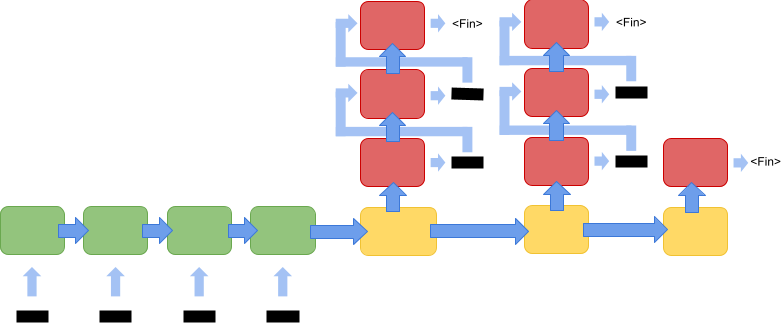
\includegraphics[scale=0.5]{2_production_mots_cles/exhird.png}
    \caption{Représentation schématique du décodage hiérarchique de la méthode ExHirD. L'encodeur du document est représenté en vert, le décodeur de concept en jaune et le décodeur de mots-clés en rouge.}
    \label{fig:schema_exhird}
\end{figure}

Dans le but de mieux modéliser les ensembles de mots-clés, \citet{chen_exclusive_2020} s'intéressent à la structure hiérarchique des ensembles de mots-clés.
En effet, les méthodes de génération de séquences de mots-clés identifient les mots-clés grâce à des marqueurs générés par le modèle. Cette séquentialité ne permet pas de représenter la hiérarchie entre les mots-clés et les mots qui les composent.
Ces travaux se rapprochent de \citet{yuan_generating_2018} qui essaient de rompre la séquentialité en modifiant la représentation des séparateurs de mots-clés avec le mécanisme de régularisation orthogonale.
Ainsi, ils présentent la méthode ExHirD~\cite{chen_exclusive_2020} dans laquelle le décodeur de l'architecture de CopyRNN est remplacé par un décodeur hiérarchique (voir figure~\ref{fig:schema_exhird}) qui génère les mots-clés en deux temps: d'abord l'identification des concepts, ensuite la génération de leur représentation textuelle.
Ce décodeur hiérarchique comprend un premier décodeur qui produit une représentation dense d'un concept, puis un second décodeur qui va générer une séquence de mots à partir de cette représentation dense pour instancier le concept en un mot-clé.
La génération des mots utilise deux mécanismes d'attention sur les documents d'entrée: l'un est conditionné par la représentation dense du concept; l'autre, standard, est conditionné par le mot précédent.
Ainsi, ce décodeur hiérarchique permet de modéliser explicitement les concepts importants du document et les mots qui les décrivent.
%
L'évaluation de cette méthode montre néanmoins un faible gain de performance, de l'ordre d'un point de F@5, pour les mots-clés présents et absents.
%
Ces travaux s'attellent aussi au problème de redondance des mots-clés et proposent un mécanisme de décodage exclusif pour tenter de le résoudre.
Ce mécanisme, simple dans son idée, interdit au modèle de générer deux mots-clés commençant par le même mot.
En effet, les mots-clés comportent le plus souvent entre 1 et 4 mots (voir section~\ref{sub:nature_linguistique}), ainsi le premier mot affecte grandement les suivants.
Ce mécanisme n'est pas limité à la méthode ExHirD; il peut être adapté aux différents types de décodage ou être utilisé en post-traitement.
Son évaluation montre qu'il fait significativement baisser le nombre de mots-clés dupliqués sans faire baisser les scores de F@5.

Les méthodes génératives \emph{one2many} apprennent à déterminer le nombre de mots-clés à produire mais en génèrent trop peu: catSeqD génère en moyenne 4,3 mots-clés par document alors que la référence en est composée de 5,3 en moyenne.
Les travaux de \citet{chan_neural_2019} s'intéressent à encourager les modèles à générer plus de mots-clés, en les entraînant à optimiser le rappel et la \fmesure{}.
Or ces métriques ne peuvent être utilisées comme fonction de coût dans l'algorithme de descente de gradient, car elles ne sont pas dérivables.
Pour résoudre ce problème, les auteurs proposent d'utiliser l'apprentissage par renforcement pour affiner\footnote{\foreign{To fine-tune} en anglais.} des modèles déjà entraînés.
%
Dans l'apprentissage par renforcement~\cite{williams_simple_1992}, un agent produit une série d'actions en suivant une politique (ici la génération de mots grâce à un modèle génératif), puis est récompensé pour chacune des actions.
%Dans l'apprentissage par renforcement~\cite{williams_simple_1992}, un agent produit une série d'actions en suivant une politique puis il est récompensé pour chaque action.
%Dans notre cas, une action consiste à générer un mot, la politique permettant de choisir le mot est un modèle génératif, et la récompense est le rappel ou la f-mesure.
L'algorithme d'apprentissage par renforcement optimise ainsi les poids du modèle (met à jour la politique) en fonction de la récompense.
%
Dans la méthode proposée, la récompense s'adapte selon le nombre de mots-clés générés: s'il est trop faible, la récompense sera le rappel pour encourager le modèle à générer plus de mots-clés; à l'inverse s'il est trop grand, la récompense sera la \fmesure{}, pour encourager le modèle à générer seulement de bons mots-clés.
%
De plus, les mots-clés présents et absents sont récompensés séparément pour favoriser la génération des mots-clés absents.

%CDKGen~\cite{diao_keyphrase_2020} (use close docs to encode, transformers)
%SenseNet~\cite{luo_sensenet_2020} (??)

Les travaux, concernant les méthodes neuronales, présentés jusqu'à présent considèrent que la quantité de données disponibles est suffisante.
Nous verrons dans le chapitre~\ref{chap:framework} que les sources de données contenant des documents annotés en mots-clés sont peu nombreuses malgré la large disponibilité de documents scientifiques en ligne.
Ainsi, les travaux de \citet{ye_semi-supervised_2018} se placent dans un cadre où la quantité de documents annotés est limitée.
%
Pour cela, les auteurs proposent deux méthodes qui tirent parti de la masse de documents non annotés pour la génération de mots-clés.
%
La première méthode consiste à utiliser des documents non annotés en mots-clés dans le cadre d'apprentissage multitâche.
Un réseau de neurones encodeur-décodeur est entraîné, pour les documents annotés, à générer des séquences de mots-clés et, pour les documents non annotés, à générer le titre du document. Dans le modèle, deux décodeurs différents sont utilisés pour chacune des tâches mais l'encodeur est partagé.
%
La seconde méthode consiste à créer un corpus synthétique en annotant automatiquement des documents en mots-clés. Les mots-clés sont extraits grâce aux méthodes \tfidf{} et TextRank.
Ainsi, un modèle de génération de mots-clés est pré-entraîné grâce à la combinaison des corpus synthétique et annoté, puis affiné grâce au seul corpus annoté.
%
L'évaluation des deux modèles résultant de ces méthodes d'entraînement montre qu'ils obtiennent des résultats similaires.
Les scores de F@5 pour les mots-clés présents des modèles semi-supervisés sont comparables à ceux du modèle \emph{catSeq} (CopyRNN entraîné à générer des séquences de mots-clés), bien qu'ils n'utilisent qu'un dixième des documents annotés utilisés par \emph{catSeq}.

\subsection{Extraction de mots-clés}

% Chapeau
Les méthodes génératives de bout-en-bout sont très performantes pour produire des mots-clés présents, mais génèrent très peu de mots-clés absents.
Ainsi, la communauté scientifique s'intéresse à des méthodes de bout-en-bout exclusivement extractives.
%Les méthodes génératives de bout-en-bout sont très performantes pour produire des mots-clés présents, ainsi la communauté scientifique s'intéresse à 
%Les méthodes génératives de bout-en-bout, qui ont la particularité de produire des mots-clés absents, n'en produisent au final que très peu~\cite[inter alia]{chen_exclusive_2020, santosh_hicova_2021} et ceux-ci ne correspondent que très peu aux mots-clés de référence~\cite[inter alia]{ahmad_select_2020, ye_one2set_2021}.
%Mais leurs performances élevées pour produire des mots-clés présents encouragent tout de même le développement de méthodes de bout-en-bout.
%C'est pourquoi la communauté scientifique s'intéresse aux méthodes de bout-en-bout exclusivement extractives.
%
Bien qu'elles ne soient pas au c\oe{}ur de nos travaux, nous présentons les principales méthodes extractives par soucis d'exhaustivité.
% Plan
Dans cette section nous présentons tout d'abord les méthodes fondées sur l'annotation en séquence, ensuite, une méthode de classification, et enfin, une méthode fondée sur les graphes.

Le développement de ces méthodes est lié à celui des modèles de langues pré-entraînés tels que BERT~\cite{devlin_bert_2019}, SciBERT~\cite{beltagy_scibert_2019} ou encore GPT-2~\cite{radford_language_2019} qui reposent sur l'architecture transformer~\cite{vaswani_attention_2017}.
Ils sont utilisés pour fournir des plongements de mots contextuels ou bien pour être affinés pour une tâche particulière.
Ces modèles, entraînés sur de très grandes quantités de données, ont permis d'améliorer significativement les performances de nombreuses tâches de traitement automatique de la langue~\cite{wang_glue_2018}.

% Annotation en séquence
\paragraph{Annotation en séquence}
La grande majorité des méthodes extractives de bout-en-bout reformulent la tâche de production de mots-clés en une tâche d'annotation en séquence.
Dans l'annotation en séquence, chaque mot du document est associé à une étiquette selon un schéma binaire: mot-clé ou non mot-clé, ou bien selon le schéma \texttt{BIO} dans lequel les mots du document correspondent au début (\texttt{B}), à l'intérieur (\texttt{I}) ou à l'extérieur (\texttt{O}) d'un mot-clé.\\
%
La méthode pionnière, proposée par \citet{augenstein_multi-task_2017}, utilise un encodeur récurrent bi-directionnel pour représenter chacun des mots et prédire leurs étiquettes.
Elle est amélioré par \citet{alzaidy_bi-lstm-crf_2019} qui ajoute un champ aléatoire conditionnel (CRF) pour améliorer la prédiction séquentielle des étiquettes, ainsi que par \citet{sahrawat_keyphrase_2019} qui utilise les plongements contextuels de BERT en entrée de l'encodeur.
%
La méthode SaSaKe~\cite{santosh_sasake_2020}, quant à elle, utilise les relations de dépendances syntaxique et sémantique du document pour améliorer la représentation des mots.
Le document est encodé puis les relations de dépendances sont représentées sous formes de graphes et incorporées aux représentations des mots grâce à des réseaux à convolution de graphes.
Ces représentation servent ensuite à étiqueter chaque mot comme mot-clé ou non mot-clé.
%La méthode pionnière, proposée par \citet{augenstein_multi-task_2017}, utilise un encodeur récurrent bi-directionnel pour représenter chacun des mots et prédire leurs étiquettes. D'autres travaux améliorent cette méthode, notamment BiLSTM-CRF~\cite{alzaidy_bi-lstm-crf_2019} qui ajoute à l'encodeur un champ aléatoire conditionnel (CRF), ce qui améliore la prédiction séquentielle des étiquettes. Dans la même ligne de recherche, \citet{sahrawat_keyphrase_2019} améliore BiLSTM-CRF en utilisant les plongements de mots contextuels de BERT en entrée de l'encodeur.\\
%
%D'autres méthodes pour l'annotation en séquence sont présentées, la méthode SaSaKe~\cite{santosh_sasake_2020} par exemple, prend explicitement en compte la syntaxe et la sémantique des documents grâce à leurs graphes de dépendances syntaxique et sémantique. Cette méthode encode le document grâce à un transformer puis incorpore à la représentation de chaque mot les informations des graphes de dépendances à l'aide de réseaux à convolution de graphe.\\
%
%De son côté, \citet{martinc_tnt-kid_2020} propose la méthode TNT-KID qui tire parti du transfert de connaissances d'un modèle de langue pré-entraîné et se place dans un contexte de données limitées. Cette méthode consiste d'abord à pré-entraîner un modèle de langue transformer à l'aide de données non annotées. Puis à affiner ce modèle grâce au seul ensemble de validation de KP20k pour l'identification de mots-clés grâce à l'annotation en séquence. Ainsi, avec seulement \num{20000} documents annotés cette méthode obtient des résultats comparables à ceux de CopyRNN.

% Classification
\paragraph{Classification}
La méthode BERT-JointKPE~\cite{sun_joint_2020} s'inspire des méthodes en chaîne de traitement pour entraîner un modèle de bout-en-bout à classifier chaque n-gramme du document comme mot-clé ou non mot-clé. Cette méthode ressemble donc à une sélection de mots-clés candidats n-grammes (voir section~\ref{selection-des-mots-cles-candidats}).
Les plongements des mots du document sont d'abord calculés à l'aide de BERT. Ensuite, grâce à des convolutions de différentes tailles, les représentations des mots sont agrégées pour représenter les n-gramme (de 1 à 5).
Enfin, chaque n-gramme est classifié comme mot-clé ou non mot-clé grâce à sa représentation dense.

% Enfin
\paragraph{Graphe}
La méthode DivGraphPointer~\cite{sun_divgraphpointer_2019} diffère des autres méthodes extractives car elle est fondée sur le paradigme encodeur-décodeur.
Nous la décrivons en détail pour comparer son architecture à celles des méthodes génératives décrites dans les sections~\ref{sub:generation_de_mots_cles} et \ref{sub:generation_de_sequences_de_mots_cles}.
%
Cette méthode combine la représentation sous forme de graphe, largement utilisée par les méthodes en chaîne de traitement (voir section~\ref{graphe}), et la génération de mots-clés en séquence (\emph{one2many}).%
\footnote{Cette méthode est générative, mais ne peut produire de mots-clés absents. En dehors de sa description nous réservons le terme \say{méthodes génératives} aux seules méthodes pouvant produire des mots-clés absents.}
L'intérêt de cette représentation est double: elle permet premièrement de mutualiser l'information des multiples occurrences d'un même mot; et deuxièmement, elle permet de prendre en compte les interactions entre les mots de manière globale.
%
Ainsi, le document est d'abord représenté sous forme de graphe dans lequel les n\oe{}uds représentent les mots et les arêtes la distance entre les positions des mots.
Ensuite, des couches de convolution de graphe calculent la représentation de chaque n\oe{}ud en fonction de ses voisins.
Ces représentations sont agrégées pour initialiser le décodeur, un \foreign{pointer network}~\cite{vinyals_order_2016}.
Enfin, ce décodeur produit une séquence de mot exclusivement copiée du document.
%
DivGraphPointer à pour objectif, comme \emph{catSeqD}, de produire des mots-clés peu redondants.
Ainsi, en plus du mécanisme d'attention et de couverture, le mécanisme de \emph{modification du contexte} (similaire dans son objectif à la \emph{régularisation orthogonale} de \emph{catSeqD}) recalcule l'état caché après avoir généré un séparateur de mot-clé.
Cet état caché est calculé en fonction de la représentation du document et de l'ensemble des mots-clés précédemment générés.\\
%
Un intérêt peu discuté de cette méthode est sa capacité à produire des mots-clés qui ne sont pas des sous-séquences du document mais dont tous les mots y apparaissent.
Ainsi, la dichotomie entre mots-clés présents et mots-clés absents ne semble ne pas convenir à ce type de mots-clés.
Nous discuterons la définition de mots-clés présents et de mots-clés absents dans le chapitre~\ref{chap:ri}.


\section{Conclusion}

% Méthodes en ch de traitement
%Nous avons vu dans le chapitre~\ref{chap:concepts} les méthodes de production automatique de mots-clés en chaîne de traitement.
%La communauté scientifique à proposé de nombreuses méthodes en chaîne de traitement qui utilisent différents descripteurs pour identifier les mots-clés les plus importants des documents.
%Ces méthodes nécessitent peu de données d'entraînement ou sont non supervisées.
%Elles ne dépendent généralement pas de la langue et peuvent être transposées simplement.
%
%Malheureusement, l'enchaînement des différentes étapes propage et intensifie les erreurs.
%De plus, la définition manuelle des descripteurs, qui nécessite des connaissances expertes, limite la transférabilité des méthodes à d'autres types de document.
%Enfin, ces méthodes en chaîne de traitement, majoritairement extractives, ne peuvent produire que des mots-clés qui sont présents dans le document.
%
%Pour pallier la propagation d'erreurs et la définition manuelle des descripteurs, des méthodes d'apprentissage profond de bout-en-bout sont proposées.
%Malgré leurs avantages, ces méthodes nécessitent d'être entraînées à l'aide de grandes quantités de données annotées.
%
%Ces méthodes sont cependant moins généralisables à d'autres genres de documents de par leur nature supervisée, ainsi qu'à d'autres langues car elles nécessitent des données annotées.
%
%De plus, leur complexité, leur variabilité dans leurs implémentations, leur temps d'exécution et d'entraînement sont aussi des limites à leur utilisation à grande échelle.
%paramètres à prendre en compte en fonction de l'utilisation qui en sera faite.

Dans ce chapitre, nous avons présenté les principes fondamentaux des réseaux de neurones ainsi que le paradigme encodeur-décodeur qui permet d'encoder un document de longueur variable et de générer une séquence de mots.
Nous avons ensuite présenté un état de l'art des méthodes de production de mots-clés de bout-en-bout, toutes neuronales, qui reposent à minima sur les encodeurs ou les décodeurs.
Pour cet état de l'art, nous avons séparé ces méthodes en deux catégories~: les méthodes génératives et les méthodes extractives.


% 2.1 fondements
% 2.1.1 neural nets
% 2.1.2 encodage
% 2.1.3 décodage
% 2.1.4 stratégies de décodages
% 2.1.5 encodeur-décodeur

La mise à disposition, par \citet{meng_deep_2017}, d'une grande quantité de données annotées permet le développement de méthodes de bout-en-bout pour la production de mots-clés.
Ces méthodes de bout-en-bout pallient certains écueils des méthodes en chaîne de traitement, présentées au chapitre~\ref{chap:concepts}, notamment la propagation des erreurs entre les différentes étapes et la définition manuelle des traits pour identifier l'importance des mots-clés.
%
Néanmoins, les méthodes de bout-en-bout ne sont pas exemptes de limites~: elles nécessitent de grandes quantités de données pour être entraînées ainsi qu'une grande puissance de calcul pour être utilisées.
%Elles introduisent néanmoins de nouvelles limitations: premièrement, la nécessité de disposer de grandes quantités de données annotées pour leur entraînement et deuxièmement, la disposition d'une grande puissance de calcul nécessaire à leur exécution.

Les méthodes extractives de bout-en-bout s'inspirent, pour la majorité, de l'annotation en séquence et entraînent des réseaux de neurones à identifier le début et la fin des mots-clés dans les documents.
Ces méthodes sont, de manière générale, plus performantes que les méthodes génératives, ainsi, la spécialisation des méthodes dans l'extraction de mots-clés semble faciliter la tâche.

%Les méthodes génératives, qui constituent le c\oe{}ur de nos travaux, entraînent un réseau de neurones à générer les mots-clés de référence.
%Ces méthodes ont la capacité de produire des mots-clés absents, ce que les méthodes proposées jusqu'alors ne permettaient pas.
%Cependant, l'analyse des mots-clés générés par ces méthodes montre que les mots-clés qui correspondent à la référence sont presque exclusivement des mots-clés présents.
%Ainsi, elles ne produisent en fait que très peu de mots-clés absents et ceux-ci ne correspondent que très peu à la référence.
%Nous verrons dans le chapitre~\ref{chap:ri} que ces mots-clés absents sont un enjeu important pour la tâche de recherche d'information.

Les méthodes génératives, qui constituent le c\oe{}ur de nos travaux, entraînent un réseau de neurones à générer les mots-clés de référence.
Elles ont la capacité de produire des mots-clés absents, ce que les méthodes proposées jusqu'alors ne permettaient pas.
Ces méthodes ont deux principales faiblesses: elles produisent très peu de mots-clés absents (1,7 en moyenne~\cite{chan_neural_2019}) et produisent des mots-clés très redondants (entre  \npercent{20} et \npercent{30}~\cite{chen_exclusive_2020}).
%
Ainsi, les différentes méthodes présentées ont pour objectif de pallier au moins une de ces faiblesses en ajoutant des mécanismes de diversification des mots-clés, en essayant d'améliorer la modélisation des documents ou en modifiant le processus de décodage.
De manière globale, les performances de la tâche de production automatique de mots-clés augmentent peu.
Notons tout de même l'amélioration des performances pour les mots-clés \emph{présents} de 33 à 40 points de F@5 sur KP20k entre les premiers travaux de \citet{meng_deep_2017} et ceux, plus récents, de \citet{ye_heterogeneous_2021}.
%La production de mots-clés présents augmente tout de même: les premiers travaux de \citet{meng_deep_2017} et ceux, plus récents, de \citet{ye_heterogeneous_2021} rapportent respectivement une F@5 sur KP20k de 33 et de 40 points.
%Mais la production de mots-clés absents, elle, stagne: \citet{chan_neural_2019} et \cite{ye_heterogeneous_2021} rapportent respectivement une F@5 sur KP20k de 1,5 et 3.
Mais, malgré cette augmentation de performance pour les mots-clés présents, les performances pour les mots-clés \emph{absents} ne dépassent pas 5 points de F@5~\cite{chan_neural_2019,ye_heterogeneous_2021}.
%
Nous verrons dans le chapitre~\ref{chap:ri} que ces mots-clés absents sont un enjeu important pour la tâche de recherche d'information.


%Premièrement, elles produisent très peu de mots-clés absents (1,7 en moyenne contre 3,9 pour les mots-clés présents ~\cite{chan_neural_2019}) et ceux-ci ne correspondent que très peu à la référence (avec une F@5 maximale de 3,6 atteinte par \citet{ye_one2set_2021}).
%Deuxièmement, les mots-clés générés sont très redondants, ceux-ci prennent la place de bon mots-clés possible \citet{chen_exclusive_2020} estime qu'entre \npercent{20} et \npercent{30} des mots-clés produits sont redondants.


%Les principaux problèmes des méthodes générative sont que les mots-clés produits sont très redondants, et que très peu de mots-clés absents sont effectivement généré (qu'ils correspondent à la référence ou pas).
%Ainsi les différentes méthodes présentées ont pour objectif de pallier l'un de ces problèmes en ajoutant des mécanisme ou en modifiant le processus d'entraînement des modèles.
%Les améliorations en terme de \fmesure{} de chaque méthode sont peu significatives.
%
%Les méthodes d'annotation en séquence, quant à elles, sont de manière générales plus performantes que les méthodes génératives.
%Ainsi, la spécialisation des méthodes dans l'extraction de mots-clés semble faciliter la tâche.
%Elles obtiennent, sur KP20k, des scores de l'ordre de 45 points de \fmesure{} pour les mots-clés présents, ce qui est supérieur aux méthodes génératives qui, pour l'instant, obtiennent des scores toujours inférieurs à 40 points de \fmesure{}.


\backmatter
\cleardoublepage
\chapter{Production de mots-clés de bout-en-bout} \label{chap:kw_production}

Ce chapitre présente les méthodes de production de mots-clés de l'état de l'art de bout-en-bout, qui constituent l'élément principal de ce travail de thèse. 
Nous commencerons par présenter les composants de ces méthodes auxquels nous feront référence dans la partie état de l'art.

\section{Principes fondamentaux des réseaux de neurones}
% Fondements sur les réseaux de neurones

Nous présentons dans cette section les concepts nécessaires à la bonne compréhension des méthodes de production de mots-clés de bout-en-bout.
Nous décrivons d'abord en détail les réseaux de neurones, ensuite les plongements de mots (\foreign{word embeddings}) utilisés pour représenter les mots du langage naturel, et enfin le paradigme encodeur-décodeur qui permet de traiter du texte de longueur variable en entrée et en sortie des réseaux de neurones.

Contrairement aux méthodes en chaîne de traitement décrites dans la section~\ref{sec:methode-en-chaine-de-traitement}, les méthodes de bout-en-bout, qui utilisent le paradigme encodeur-décodeur, se passent de l'identification des candidats ainsi que du choix des caractéristiques des mots-clés qui serviront à les pondérer.
En effet, les méthodes que nous décrivons dans ce chapitre utilisent des réseaux de neurones profonds qui apprennent à extraire automatiquement les descripteurs  les plus pertinents.
%L'apprentissage profond, permet de laisser le modèle extraire les descripteurs de manière automatique au lieu de les définir à la main, ce qui nécessite des connaissances expertes. Mais cela est difficile à interpreter, tout un pan de la recherche s'intéresse à expliquer ces méthodes (blackbox nlp)~\cite{}.


\subsection{Réseaux de neurones}
\label{sub:neural_network}

\begin{figure}
    \centering
    %Heavily inspired from https://texample.net/tikz/examples/neural-network/

\begin{tikzpicture}[shorten >=1pt,->,draw=black!50]
    \def\myscale{1.5}
    \tikzstyle{neuron}=[circle,fill=black!25,minimum size=17*\myscale,inner sep=0cm]
    \tikzstyle{input neuron}=[neuron, fill=color1!60];
    \tikzstyle{hidden neuron}=[neuron, fill=color0!60];
    \tikzstyle{output neuron}=[neuron, fill=color2!60];
    \tikzstyle{edge label}=[above=-.025cm,sloped,scale=.4*\myscale,black!60]
    \tikzstyle{label}=[scale=.75*\myscale, text width=2cm, align=center]

    \def\layersep{2.5*\myscale}
    \def\ninput{2}
    \def\nlayerone{3}
    \def\nlayertwo{2}
    \def\noutput{2}

    % Draw the input layer nodes
    \foreach \name / \y in {1,...,\ninput}
    % This is the same as writing \foreach \name / \y in {1/1,2/2,3/3,4/4}
        \node[input neuron] (I-\name) at (0,-\y*\myscale) {};


    % Draw the hidden layer nodes
    \foreach \name / \y in {1,...,\nlayerone}
        \path[yshift=.5*\myscale cm]
            node[hidden neuron] (H1-\name) at (1*\layersep,-\y*\myscale) {};

    \foreach \name / \y in {1,...,\nlayertwo}
        \path[yshift=.0*\myscale cm]
            node[hidden neuron] (H2-\name) at (2*\layersep,-\y*\myscale) {};

    % Draw the output layer node
    \foreach \name / \y in {1,...,\noutput}
        \path[yshift=0*\myscale cm]
            node [output neuron] (O-\name) at (3*\layersep,-\y*\myscale) {};

    % Connect every node in the input layer with every node in the
    % hidden layer.
    
    %\foreach \source in {1,...,\ninput}
    %    \foreach \dest in {1,...,\nlayerone}
    %        \draw[->] (I-\source) -- node [edge label, pos={.28-}] {$W^1_{\source,\dest}$} (H1-\dest);
    
    \def\layerout{1}
    \def\source{1}
    \foreach \dest / \n in {1/.2,2/.25,3/.235}
        \draw[->] (I-\source) -- node [edge label, pos={\n}] {$W^\layerout_{\source,\dest}$} (H\layerout-\dest);
    \def\source{2}
    \foreach \dest / \n in {1/.17,2/.285,3/.26}
        \draw[->] (I-\source) -- node [edge label, pos={\n}] {$W^\layerout_{\source,\dest}$} (H\layerout-\dest);


    \def\layerout{2} % modify this
    \pgfmathtruncatemacro{\layerin}{\layerout - 1}
    \def\source{1} % modify this
    \foreach \dest / \n in {1/.2,2/.26} % modify this
        \draw[->] (H\layerin-\source) -- node [edge label, pos={\n}] {$W^\layerout_{\source,\dest}$} (H\layerout-\dest);
    \def\source{2} % modify this
    \foreach \dest / \n in {1/.2,2/.25} % modify this
        \draw[->] (H\layerin-\source) -- node [edge label, pos={\n}] {$W^\layerout_{\source,\dest}$} (H\layerout-\dest);
    \def\source{3} % modify this
    \foreach \dest / \n in {1/.23,2/.3} % modify this
        \draw[->] (H\layerin-\source) -- node [edge label, pos={\n}] {$W^\layerout_{\source,\dest}$} (H\layerout-\dest);

    % Connect every node in the hidden layer with the output layer
    \def\layerout{3} % modify this
    \pgfmathtruncatemacro{\layerin}{\layerout - 1}
    \foreach \source in {1,...,\nlayertwo}
        \foreach \dest in {1,...,\noutput}
            \draw[->] (H\layerin-\source) -- node [edge label, pos={.20+(1-Mod(\dest,2))*.05}] {$W^\layerout_{\source,\dest}$} (O-\dest);

    % Annotate the layers
    \node[label, below=.1cm of I-\ninput] (I-label) {Entrée};

    \node[draw, dashed, rounded corners,fill=none, fit=(H1-1) (H1-\nlayerone)] (H1) {};
    \node[label, below=.1cm of H1] (H1-label) {Première couche};

    \node[draw, dashed, rounded corners,fill=none, fit=(H2-1) (H2-\nlayertwo)] (H2) {};
    \node[label, below=.1cm of H2] (H2-label) {Seconde couche};

    \node[draw, dashed, rounded corners,fill=none, fit=(O-1) (O-\noutput)] (O) {};
    \node[label, below=.1cm of O] (O-label) {Couche de sortie};

    \node[draw, dashed, rounded corners,fill=none, fit=(H1) (H1-label) (H2) (H2-label)] (H) {};
    \node[label, text width=10cm, below=.1cm of H] (H-label) {Couches cachées};

\end{tikzpicture}
    \caption{Représentation graphique d'un réseau de neurones à 2 couches. Les flèches représentent les poids des matrices $W^k$. Les biais $b^k$ ne sont pas représentés.}
    \label{fig:ex_nn_simple}
\end{figure}
% https://texample.net/tikz/examples/neural-network/

Les réseaux de neurones servent à modéliser des fonctions complexes, qui peuvent être non linéaires.
%
D'un point de vue mathématique, il s'agit de modéliser une fonction $f$ qui prend une entrée $X$ et retourne une sortie (une prédiction) $\hat{Y} = f(X)$.
%
Ici, $X \in M_{1,m}(\mathds{R})$ et $\hat{Y} \in M_{1,n}(\mathds{R})$ sont des vecteurs de taille $m$ et $n$ respectivement.
%
Ces vecteurs représentent le nombre de paramètres d'entrée de la fonction $f$.
%
%Par exemple, un modèle qui prédit le prix d'une maison en fonction de sa surface et du nombre de fenêtres aura 2 entrées et une sortie.


Un réseau de neurones simple (également appelé perceptron mono-couche) est défini par l'équation~\ref{eq:simple_nn} ci-dessous, dans laquelle $W$ est une matrice de poids $W \in M_{m, n}(\mathds{R})$ et $b$ un vecteur de biais $b \in M_{1,m}(\mathds{R})$.
%
\begin{align}
    \hat{Y} = f(X) = \sigma (b + W * X) \label{eq:simple_nn}
\end{align}


La fonction $\sigma$ est une fonction dite d'activation.
Elle est inspirée de l'activation des neurones dans le cerveau humain.
L'information d'un neurone passe à la couche suivante si le neurone est activé (c'est-à-dire si sa valeur est assez élevée).
Les fonctions Sigmoïde (voir équation~\ref{eq:sigmoide}) et Rectified Linear Unit (ReLU) (voir équation~\ref{eq:relu}) sont généralement utilisées pour $\sigma$.
%Cette fonction est généralement la fonction sigmoïde (équation~\ref{eq:sigmoide}), Rectified Linear Unit (ReLU) (équation~\ref{eq:relu}), ou tangente hyperbolique ($\text{tanh}$). \todo{comment choisir cette fonction ?}

\begin{gather}
    \sigma(x) = \frac{1}{1+e^{-x}} \label{eq:sigmoide} \\
    \textsc{ReLu}(x) = \text{max}(0, x) \label{eq:relu}
\end{gather}

%\begin{figure}\centering
%    \begin{tikzpicture}\begin{axis}[xmin=-5, xmax=5, ymin=-2, ymax=2]
%        \addplot {1/(1+e^(-x))};
%        \addplot {tanh(x)};
%        \addplot {max(x, 0};
%    \end{axis}\end{tikzpicture}
%    \caption{Caption} \label{fig:my_label}
%\end{figure}

Un réseau de neurones à une couche (perceptron mono-couche) ne peut modéliser que des fonctions linéaires, et ne pourra jamais modéliser une fonction telle que la fonction XOR par exemple~\cite{minsky_perceptrons_1988}.
Pour gagner en expressivité, des couches de neurones sont ajoutées (voir figure~\ref{fig:ex_nn_simple}). Un tel réseau de neurones est aussi appelé perceptron multicouche.
%
Un perceptron mono ou multicouche dénote un réseau de neurones à propagation avant (\foreign{feed forward neural network}) où chaque couche est entièrement connectée à la suivante.

En utilisant les perceptrons multicouche, il est possible de modéliser des fonctions plus complexes.
Dans ce cas, chaque couche utilise la sortie de la couche précédente comme entrée (voir équation~\ref{eq:multi_nn}).
La couche \num{0} représente l'entrée du réseau, $k$ représente une couche intermédiaire et $n$ la couche de sortie.
Les matrices $W$ (et leur vecteurs de biais) définissent la taille de chaque couche (c'est-à-dire le nombre de neurones).
En effet, une matrice de taille $n*m$ (et un vecteur $b$ de taille $m$) définit une couche de taille $m$, $n$ étant conditionné par la taille de la couche précédente.
%
\begin{equation}\label{eq:multi_nn}
  \begin{split}
    h^0 & = X \\
    h^k & = \sigma(b^k + W^k * h^{k-1}) \\
    \hat{Y} & = h^n
  \end{split}
\end{equation}

Entraîner le réseau de neurones $f$ consiste à modifier les paramètres du modèle $\theta$ (matrices de poids $W^k$ et $b^k$) afin de minimiser l'erreur de prédiction. Cette erreur est définie par une fonction de coût (\emph{loss function}) $\mathcal{L}$ (voir équation~\ref{eq:loss}) calculé grâce à une prédiction $\hat{Y} = f(X)$ et une vérité terrain $Y$.
Le but de l'entraînement est de minimiser cette fonction de coût pour tous les exemples d'un jeu de données, dénoté par l'équation~\ref{eq:loss_dataset}.
%
\begin{gather} 
    \text{erreur} = \mathcal{L}(\hat{Y}, Y) = \mathcal{L}(f(X, \theta), Y) \label{eq:loss} \\
    \text{min}_\theta \sum_{(x, y) \in \mathcal{D}} \mathcal{L}(f(x, \theta), y) \label{eq:loss_dataset}
\end{gather}

L'algorithme utilisé pour minimiser la fonction de coût dans le cadre des réseaux de neurones est la descente de gradient~\cite{curry_method_1944} (Gradient Descent).
Le gradient de la fonction de coût donne la direction dans laquelle modifier les paramètres (ici les poids du réseau de neurones) pour minimiser ce coût.
Cet algorithme calcule le gradient avec tous les exemples du jeu de données puis met à jour les poids du réseau; ce processus est donc très long. Pour pallier cette lenteur, la descente de gradient par minibatch calcule le gradient à l'aide d'un nombre fixe d'exemples qui fait un compromis entre temps de calcul et utilisation d'un grand nombre d'exemples.
% figure 
%Cet algorithme utilise le fait que la fonction de coût et le réseau de neurones soient dérivables pour calculer le gradient de l'erreur et modifier les poids par rétro-propagation pour minimiser l'erreur.

Les réseaux de neurones que nous venons de décrire fonctionnent avec une entrée de taille fixe $X$; or dans le cas du texte, les entrées sont des séquences de mots de longueur variable, et n'ont donc pas de longueur fixe. Nous présentons dans la suite de cette section une architecture permettant de traiter les entrées de longueur variable.

\subsection{Encodage de séquences (encodeur)}
\label{sub:encoding}

\subsubsection{Représentation dense des mots}
\label{sec:word_embedding}

Les réseaux de neurones manipulent des vecteurs et des matrices de nombres. Le langage naturel étant constitué par des mots, il est nécessaire de transformer les mots en nombres.
Pour cela, un vocabulaire qui associe un nombre à chacun des mots est nécessaire. La méthode la plus simple est de considérer les mots les plus fréquents d'un ensemble de documents d'entraînement comme le vocabulaire $\mathcal{V}$.
Un vocabulaire de taille trop importante peut être difficile à modéliser et contiendra de nombreux hapax\footnote{Mots n'apparaissant qu'une seule fois.}. Il est donc courant de conserver les \num{50 000} mots les plus fréquents~\cite{meng_deep_2017,yuan_one_2020,ye_one2set_2021}.
%Plusieurs techniques sont utilisés pour représenter un document sous forme de vecteur à l'aide d'un tel vocabulaire.
%L'encodage \emph{one-hot}, crée un vecteur de la taille du vocabulaire $|\mathcal{V}|$ où chaque dimension représente la fréquence du mot correspondant dans le document. Cette méthode est peu efficiente en terme d'espace car le vecteur ainsi créé est creux (il contient une grande majorité de 0).

% exemple image
Aujourd'hui, les plongements de mots sont l'état de l'art en termes de représentation de mots. Ce sont des représentations denses apprises sur de grandes quantités de données qui modélisent les cooccurrences entre les mots: deux mots utilisés dans des contextes similaires auront des vecteurs similaires~\cite{mikolov_efficient_2013}.
Plusieurs méthodes ont été proposées pour pré-entraîner ces plongements.
Les méthodes précurseures word2vec~\cite{mikolov_efficient_2013} et gloVe~\cite{pennington_glove_2014} calculent des représentations fixes des mots. Leurs principales lacunes sont la prise en compte de mots hors du vocabulaire et la prise en compte de la polysémie. Pour prendre en compte les mots hors du vocabulaire, fastText~\cite{bojanowski_enriching_2017} apprend des plongements de n-grammes de caractères puis combine ceux-ci pour représenter le mot entier. Ensuite, pour traiter la polysémie, Elmo~\cite{peters_deep_2018} et Bert~\cite{devlin_bert_2019} calculent ces plongements en fonction du contexte des mots.
Il est aussi possible d'entraîner des plongements à l'aide d'une simple matrice de poids au début du réseau de neurones. Dans la tâche de génération de mots-clés, cette technique est la plus utilisée.


\subsubsection{Encodeurs}

Les encodeurs sont des réseaux de neurones qui permettent de traiter des séquences de longueur variable. Dans nos travaux ces séquences sont des documents textuels.
Les encodeurs prennent en entrée une séquence de vecteurs, ici des plongements de mots, et donnent en sortie un vecteur de pensée qui agrège l'information de la séquence d'entrée.

Il existe différents types de réseaux permettant d'encoder une séquence: les réseaux récurrents, les réseaux à convolution, les transformers, les réseaux à convolutions de graphes.
Nous nous intéresserons ici aux encodeurs récurrents, les plus utilisés pour la génération de mots-clés. 
Un encodeur récurrent est composé d'une ou plusieurs cellules récurrentes empilées.
Une cellule récurrente $\textsc{Rnn}$ encode une séquence selon l'équation~\ref{eq:rnn}.
%
\begin{equation}\label{eq:rnn}
\begin{split}
    h_t & = \textsc{Rnn}^e(x_{t}, h_{t-1}) \\
    \textsc{Rnn}^e(x_t, h_{t-1}) & = \text{tanh}(W_x * x_t + b_x + W_h * h_{t-1} + b_h)
\end{split}
\end{equation}

Dans l'équation~\ref{eq:rnn} $x_t$ représente le plongement du mot $t$, $h_t$ l'état caché au temps $t$ qui encode la sous-séquence d'entrée jusqu'au mot $t$, $W_x$ et $W_h$ des matrices de poids et $b_x$, $b_h$ les vecteurs de biais correspondants.
Le premier état caché $h_0$ est initialisé aléatoirement.
Ces réseaux sont dits récurrents car l'état caché $h_t$ est conditionné par les états cachés précédents.

Ce type d'encodeurs peut être utilisé pour entraîner un classifieur de documents en utilisant le dernier vecteur $h_t$, par exemple dans le cadre de la catégorisation de documents~\cite{wang_disconnected_2018} ou la détection de rumeurs~\cite{ma_detecting_2016}.
Il est aussi possible d'utiliser ces encodeurs pour entraîner des modèles d'annotation en séquence qui utilisent chaque représentation $h_t$ pour prédire l'étiquette du mot, par exemple dans le cadre de la reconnaissance d'entités nommées~\cite{zukov-gregoric_named_2018}.

% long dependence \todo{parler de ça}
% bidirectionnel
% oubli du début de  la séquence
Le principal écueil des réseaux récurrents est leur difficulté à garder en mémoire les dépendances à long terme.
Pour pallier ce problème, \citet{hochreiter_long_1997}  introduit les cellules LSTM (Long Short Term Memory).
Ces cellules récurrentes contiennent des \say{portes} qui leur permettent d'apprendre à sélectionner les informations à conserver ou à oublier à chaque temps $t$.
Elles donnent en sortie un état caché $h_t$ qui représente l'information pertinente au moment $t$ ainsi qu'un vecteur de contexte $C_t$ qui contient l'ensemble de l'information que la cellule a mémorisé.
Ce mécanisme de portes permet de prendre en compte les dépendances à long terme.
Cette cellule récurrente a été améliorée, notamment par les cellules récurrentes GRU (Gated Recurrent Unit)\cite{cho_learning_2014} qui simplifient les LSTM en combinant $h_t$ et $C_t$ en un unique vecteur ainsi qu'en diminuant le nombre de paramètres utilisés, ce qui en facilite l'entraînement.

Pour améliorer l'encodage des documents et la modélisation des dépendances à long terme, \citet{schuster_bidirectional_1997} présente des encodeurs bi-directionnels.
Ceux-ci sont composés de deux encodeurs qui encodent chacun la séquence dans un sens différent, du début à la fin et inversement.
Chacun de leurs états cachés sont ensuite concaténés pour n'en former qu'un. Ainsi, les états cachés de ce type d'encodeur représentent la séquence entière centrée sur le mot $t$.
%\say{You can't cram the meaning of a whole \%\&\!\$\# sentence into a single \$\&!\#* vector!} (R. Mooney).


\subsection{Génération de séquences (décodeur)}
\label{sub:decoding}

Le processus de décodage permet de générer une séquence de mots à partir d'un vecteur de pensée. Ce vecteur de pensée résulte généralement de l'encodage d'un document (cf. section~\ref{sub:encoding}).
Comme pour l'encodage, différents types de réseaux peuvent être utilisés: les réseaux récurrents, les réseaux à convolutions ou les transformers.
Nous nous intéressons ici aux réseaux récurrents, présentés dans la section~\ref{sub:encoding}.

Un décodeur récurrent est composé d'une ou plusieurs cellules récurrentes empilées.
La génération d'une séquence consiste à utiliser les états cachés $h_t$ pour prédire un mot, c'est-à-dire à produire une distribution de probabilités sur l'ensemble du vocabulaire puis à choisir le mot le plus probable.


Le processus de décodage est décrit par l'équation~\ref{eq:rnn_decodeur} avec $y_{t-1}$ le mot prédit précédemment, $h_{t-1}$ l'état caché précédent, $W_x$ et $W_h$ des matrices de poids et leurs biais correspondant $b_x$ et $b_h$.
Le premier mot $y_0$ est initialisé par un mot spécial; l'état caché $h_0$ est un vecteur de pensée.
Puis $p(y_t | y_{1,...,t-1},h_0)$ représente la distribution de probabilités sur le vocabulaire pour le mot $t$ en fonction des mots précédents et du vecteur de pensée $h_0$; $W_v$ et $b_v$ sont une matrice de poids et son biais.


\begin{equation} \label{eq:rnn_decodeur}
\begin{split}
    p(y_t | y_{1,...,t-1},h_0) & = \textsc{Softmax}(\sigma(W_v * h_t + b_v))\\
    h_t & = \textsc{Rnn}^d(y_{t-1}, h_{t-1}) \\
    \textsc{Rnn}^d(x_t, h_{t-1}) & = \text{tanh}(W_x * x_t + b_x + W_h * h_{t-1} + b_h)
    % p(Y) = \prod p(w_t|w_{t-1},...,w_0,h)
\end{split}
\end{equation}

La génération d'une séquence de mots s'effectue mot-à-mot grâce à un algorithme de décodage.
Chaque étape de décodage consiste à produire une distribution de probabilité sur le vocabulaire de sortie $p(y_t | y_{1,...,t-1},h_0)$ et à choisir un mot $\hat{y}_t$ qui maximise cette probabilité.
Cette étape est répétée jusqu'à ce qu'un mot spécial finissant la séquence soit généré ou que la séquence soit assez longue.

L'algorithme le plus simple consiste à choisir le mot le plus probable à chaque étape mais cela ne permet de générer qu'une seule séquence.
%
Dans le cadre de la génération de mots-clés il est souhaitable de générer plusieurs mots-clés et donc plusieurs séquences.
Pour cela, c'est l'algorithme de recherche en faisceau~\cite{ow_filtered_1988}, que nous schématisons dans la figure~\ref{fig:beam_search}, qui est utilisé.
Cet algorithme consiste à décoder un nombre fixe de séquences (deux dans le schéma).
Les étapes de décodage sont effectuées pour chacun des faisceaux et les mots à générer sont choisis dans l'ensemble des mots des faisceaux.
Dans la figure~\ref{fig:beam_search}, deux mots sont choisis au départ.
Une étape de décodage est ensuite effectuée pour les deux faisceaux.
\`A la troisième étape, le préfixe \texttt{ba} n'est pas conservé car les deux séquences les plus probables sont issues du préfixe \texttt{ab}.
\`A la fin de l'algorithme, deux séquences ont été générées: \texttt{aba} et \texttt{abb}.

\begin{figure}[ht!]
    \centering
    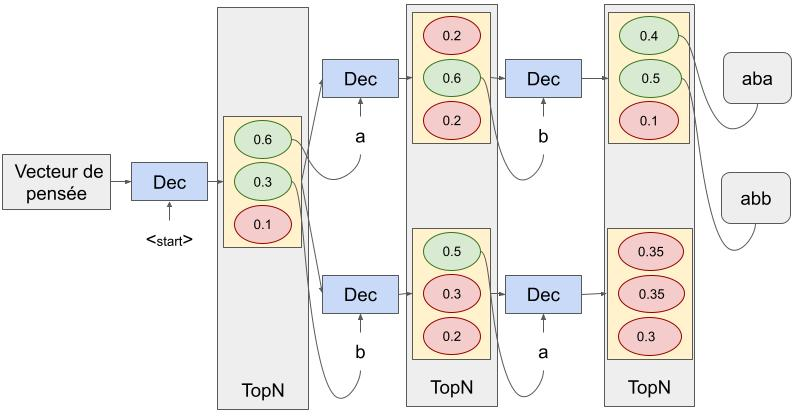
\includegraphics[scale=0.4]{2_production_mots_cles/Beam Search.jpg}
    \caption{Représentation schématique du processus de décodage grâce à l'algorithme de recherche en faisceau.}
    \label{fig:beam_search}
\end{figure}
\todo{refaire en tikz}

\`A l'inverse des algorithmes déterministes que nous avons décrits, notons l'existence des algorithmes d'échantillonnage. Ces algorithmes stochastiques choisissent les mots au hasard en fonction de leur probabilité. Les mots-clés générés par ces algorithmes ne sont donc pas reproductibles, ce qui dans le cadre de la production de mot-clés n'est pas souhaitable. Nous ne considérons donc pas cette technique.

\subsection{Paradigme encodeur-décodeur}\label{sub:paradigme_encodeur_decodeur}

Nous avons présenté dans les sections~\ref{sub:encoding} et \ref{sub:decoding} des moyens d'encoder des documents ainsi que des moyens de générer des séquences.
De nombreuses applications du traitement automatique de la langue nécessitent à la fois l'encodage d'une séquence et son décodage.
Par exemple dans le cadre de la traduction automatique, étant donnée une phrase en langue source, il faut la traduire dans une langue cible, c'est-à-dire qu'il faut encoder la phrase dans la langue source puis générer une phrase correspondante dans la langue cible.
Dans le cadre de la production de mots-clés, il faut générer un mot-clé en fonction d'un document.
Ainsi, le paradigme encodeur-décodeur introduit par \citet{sutskever_sequence_2014}, qui concatène un encodeur et un décodeur, permet de prendre en entrée une séquence de mots de longueur variable et de générer en sortie une autre séquence de mots de longueur variable.
Ce paradigme pallie la limite des réseaux de neurones présentés dans la section~\ref{sub:neural_network} (perceptrons mono ou multicouches) dont l'entrée et la sortie sont de taille fixe.

%Une fois une séquence encodée il est possible de la décoder, c'est-à-dire de produire un mot en fonction d'une représentation $h^t$.
%Générer un mot à partir d'une représentation $h_t$ consiste à passer la représentation dans un perceptron qui calcule une distribution de probabilité sur un vocabulaire, le mot à générer est choisis en fonction de sa probabilité.
    
%\begin{align}
    %\text{log}\: p(y|x) = \sum^m_{j=1} \text{log}\: p(y_j|y_{<j}, x)
%\end{align}

% FROM RECITAL SOTA

\colorlet{enccolor}{green!5}
\colorlet{inputcolor}{black!90!green}
\colorlet{deccolor}{blue!5}
\colorlet{outputcolor}{black!70!blue}
\colorlet{veccolor}{orange!15}
\colorlet{startendcolor}{black!60}
\colorlet{greybox}{black!3}

\begin{figure}[!htb]
\centering

\resizebox{\textwidth}{!}{%
\begin{tikzpicture}

\tikzstyle{cell}=[text centered, rectangle, draw, line width=.5pt, minimum height=1cm, minimum width=1.4cm, rounded corners=2pt]
\tikzstyle{word}=[font=\small\bfseries, text centered, minimum size=.5cm, minimum height=.3cm, text height=1.5ex, text depth=.25ex]
\tikzstyle{vector}=[text centered, rectangle, draw, line width=.5pt, minimum height=.5cm, minimum width=1cm, rounded corners=2pt]
\tikzstyle{arrow}=[shorten >= 2pt, shorten <= 2pt, draw=black!80]

\node[cell, fill=enccolor] (E1) at (0,0){};
\node[cell, fill=enccolor] (E2) at (2,0){};
\node[cell, fill=enccolor] (E3) at (4,0){};
\node[cell, fill=enccolor] (E4) at (6,0){};
\node[text centered] (E5) at (7.5,0){...};
\node[cell, fill=enccolor] (E6) at (9,0){};

\node[word, color=inputcolor, inner color=yellow!50, outer color=white] (I1) at (0,-1.2){Espace};
\node[word, color=inputcolor, inner color=yellow!50, outer color=white] (I2) at (2,-1.2){:};
\node[word, color=inputcolor, inner color=yellow!50, outer color=white] (I3) at (4,-1.2){la};
\node[word, color=inputcolor, inner color=yellow!50, outer color=white] (I4) at (6,-1.2){station};
%\node[word, color=inputcolor, inner color=yellow!50, outer color=white] (I5) at (8,-1.2){...};
\node[word, color=startendcolor] (I6) at (9,-1.2){<fin>};

%\node[cell, fill=veccolor, word, rotate=90] (V) at (11,0){vecteur de pensée};

\node[cell, fill=deccolor] (D1) at (11,0){};
\node[cell, fill=deccolor] (D2) at (13,0){};
\node[cell, fill=deccolor] (D3) at (15,0){};
%\node[cell, fill=deccolor] (D4) at (20,0){};

\node[word, color=startendcolor] (I7) at (11,-1.2){<début>};
\node[word, color=outputcolor, inner color=yellow!50, outer color=white] (O1) at (11,1.2){station};
\node[word, color=outputcolor, inner color=yellow!50, outer color=white] (O2) at (13,1.2){spatiale};
\node[word, color=startendcolor] (O3) at (15,1.2){<fin>};

\draw[->,>=latex,arrow] (E1) -- (E2) node[above,midway] {$h^e_0$};
\draw[->,>=latex,arrow] (E2) -- (E3) node[above,midway] {$h^e_1$};
\draw[->,>=latex,arrow] (E3) -- (E4) node[above,midway] {$h^e_2$};
\draw[->,>=latex,arrow] (E4) -- (E5) node[above,midway] {$h^e_3$};
%\draw[->,>=latex,arrow] (E5) -- (E6) node[above,midway] {$h^e_{n-1}$};
\draw[->,>=latex,arrow] (E5) -- (E6) node[above,midway] {$h^e_{n-1}$};

\draw[->,>=latex,arrow,shorten <= -2pt] (I1) to (E1);
\draw[->,>=latex,arrow,shorten <= -2pt] (I2) to (E2);
\draw[->,>=latex,arrow,shorten <= -2pt] (I3) to (E3);
\draw[->,>=latex,arrow,shorten <= -2pt] (I4) to (E4);
%\draw[->,>=latex,arrow,shorten <= -2pt] (I5) to (E5);
\draw[->,>=latex,arrow,shorten <= -2pt] (I6) to (E6);
\draw[->,>=latex,arrow,shorten <= -2pt] (I7) to (D1);


\draw[->,>=latex, arrow] (E6) -- (D1) node[above,midway] {$h^e_n$};

\draw[->,>=latex,arrow] (D1) -- (D2) node[above,midway] {$h^d_0$};
\draw[->,>=latex,arrow] (D2) -- (D3) node[above,midway] {$h^d_1$};
%\draw[->,>=latex,arrow] (D3) to (D4);

\draw[->,>=latex,arrow,shorten >= -2pt] (D1) to (O1);
\draw[->,>=latex,arrow,shorten >= -2pt] (D2) to (O2);
\draw[->,>=latex,arrow,shorten >= -2pt] (D3) to (O3);
%\draw[->,>=latex,arrow,shorten >= -2pt] (D4) to (O4);

%\node at (5,2) {\large{\textsc{Encodeur}}};
%\node at (17,2) {\large{\textsc{Décodeur}}};

\draw[arrow, rounded corners=3pt] (O1) -| (12, 0);
\draw[->,>=latex, arrow, rounded corners=3pt] (12, 0) -- (12, -1) -| (D2.south);

\draw[arrow, rounded corners=3pt] (O2) -| (14, 0);
\draw[->,>=latex, arrow, rounded corners=3pt] (14, 0) -- (14, -1) -| (D3.south);

%\draw[arrow, rounded corners=3pt] (O3) -| (19, 0);
%\draw[->,>=latex, arrow, rounded corners=3pt] (19, 0) -- (19, -1) -| (D4.south);

\draw[decoration={brace},decorate] (-0.7,1.7) -- node[below=-1.9em] {\large{\textsc{Encodeur}}} (9.7,1.7);
\draw[decoration={brace},decorate] (10.3,1.7) -- node[below=-1.9em] {\large{\textsc{Décodeur}}} (15.7,1.7);


\end{tikzpicture}
}

\caption{Exemple de modèle \textit{encodeur-décodeur} récurrent appliqué à l'extraction automatique de mots-clés.}
\label{fig:seq2seq}
\end{figure}


Le processus d'encodage et de décodage est décrit par l'équation~\ref{eq:enc-dec} et la figure~\ref{fig:seq2seq}.
Dans un premier temps la séquence d'entrée $X$ de taille $n$ est encodée dans le vecteur de pensée $h^e_n$.
Ce vecteur $h^e_n$ est utilisé pour initialiser le premier état caché du décodeur $h^d_0$.
Le décodeur génère ensuite les mots $\hat{y}_t$ qui composent la séquence de sortie $\hat{Y}$ à partir de cet état caché.

\begin{equation}\label{eq:enc-dec}
  \begin{split}
    p(\hat{y}_t | y_{1,...,t-1},h_0) & = \textsc{Softmax}(\sigma(b_v + W_v * h^d_t)) \\
    h^d_t & = \textsc{Rnn}^d(\hat{y}_{t-1}, h^d_{t-1}) \\
    \hat{y}_0 & = \textsc{Debut} \\
    h^d_0 & = h^e_n \\
    h^e_n & = \textsc{Rnn}^e(X) \\
  \end{split}
\end{equation}

Nous présentons ci-après deux améliorations de ce paradigme.
%
D'abord, le mécanisme d'attention qui permet de porter attention à une partie spécifique de l'entrée lors du décodage. Par exemple, la description d'une image nécessite d'identifier les différents objets qui la composent.
%
Ensuite, le mécanisme de copie qui pallie l'incomplétude du vocabulaire de sortie. Ce mécanisme permet au décodeur de copier un mot du document d'entrée au lieu de le générer à partir du vocabulaire de sortie. Le mécanisme de copie est particulièrement utile pour les entités nommées par exemple. Ces entités sont peu fréquentes et ne font généralement pas partie du vocabulaire de sortie.

% Convolution
%Les réseaux de neurones à convolution sont surtout utilisés pour le traitement d'images. Dans le cas du texte, des 
    
% Graphes
%Les réseaux à convolution de graphes (GCN) permettent d'obtenir pour chaque noeud d'un graphe un embedding en fonction de ses voisins. Le nombre de convolutions représente le nombre de bonds qui sont fait entre les noeuds.
    
% Transformer
%Les transformer ont été introduit par \cite{vaswani_attention_2017} et utilisent un mécanisme de self-attention pour chaque mot d'une séquence, de sorte à obtenir pour chaque mot un vecteur qui représente sa relation avec chaque autre mot. Ce mécanisme ne prend pas en compte la séquentialité, en effet chaque calcul est parallélisable. Et ce modèle qui requiert une force de calcul colossale a montré de très bons résultats sur de nombreuse tâches.

\subsubsection{Mécanisme d'attention}
\label{sub:attention_mecanism}

Le mécanisme d'attention~\cite{bahdanau_neural_2014,luong_effective_2015} a été introduit pour améliorer le traitement de longues séquences en permettant au modèle de se focaliser sur certaines parties du document lors du décodage.
%
En effet, un mot-clé concerne seulement certains aspects d'un document. Ce mécanisme permet donc au modèle de porter attention aux parties du document liées à ces aspects.
%
De plus, cette attention au document peut être visualisée grâce aux \emph{poids d'attention} calculés à chaque étape de décodage.
%Par exemple, dans le cadre de la traduction automatique, il permet de visualiser l'alignement entre la phrase en langue source et la phrase en langue cible.
%Par exemple, dans le cadre de la traduction automatique, ce mécanisme permet de visualiser l'importance de chaque mot du document source pour générer la traduction.
La figure~\ref{fig:attention_alignment} illustre cette attention dans le cadre de la traduction automatique pour traduire en français la phrase \say{The agreement on the European Economic Area was signed in August 1992.}
%Il existe généralement un alignement monotone entre les phrases en français et les phrases en anglais.
%Mais ce n'est pas toujours le cas comme le montre le syntagne nominal \say{European Economic Area} dont les mots de la traduction sont dans un ordre inverse \say{zone économique européenne}.
%Le modèle a pu, grâce au mécanisme d'attention, proposer la bonne traduction \say{zone économique européenne} dont l'ordre des mots est inverse à sa traduction.
% Même si le français et l'anglais peuvent généralemnt être traduit mot à mot de manière monotone, le mécanisme d'attention nous permet de visualiser l'alignement non monotone entre zone économique européenne et European Economic Area, en effet l'ordre des noms et adjectifs en français et en anglais est différent.
%Ainsi nous pouvons observer que pour traduire \say{was} en \say{a été}, le modèle à porté attention à \say{was signed} pour comprendre que \say{was} fait parti de la construction du prétérit.
%Pour illustrer ce mécanisme dans le cadre de la traduction automatique nous prenons l'exemple suivant: pour traduire la séquence \say{the European Economic Area} en français (\say{\foreign{la zone économique européenne}}) le modèle portera attention à chaque mot du texte source. Ainsi, pour générer \say{la} et \say{zone} il devra porter attention à \say{\foreign{the}} et \say{\foreign{Area}}. \todo{A revoir.}

\begin{figure}
    \centering
    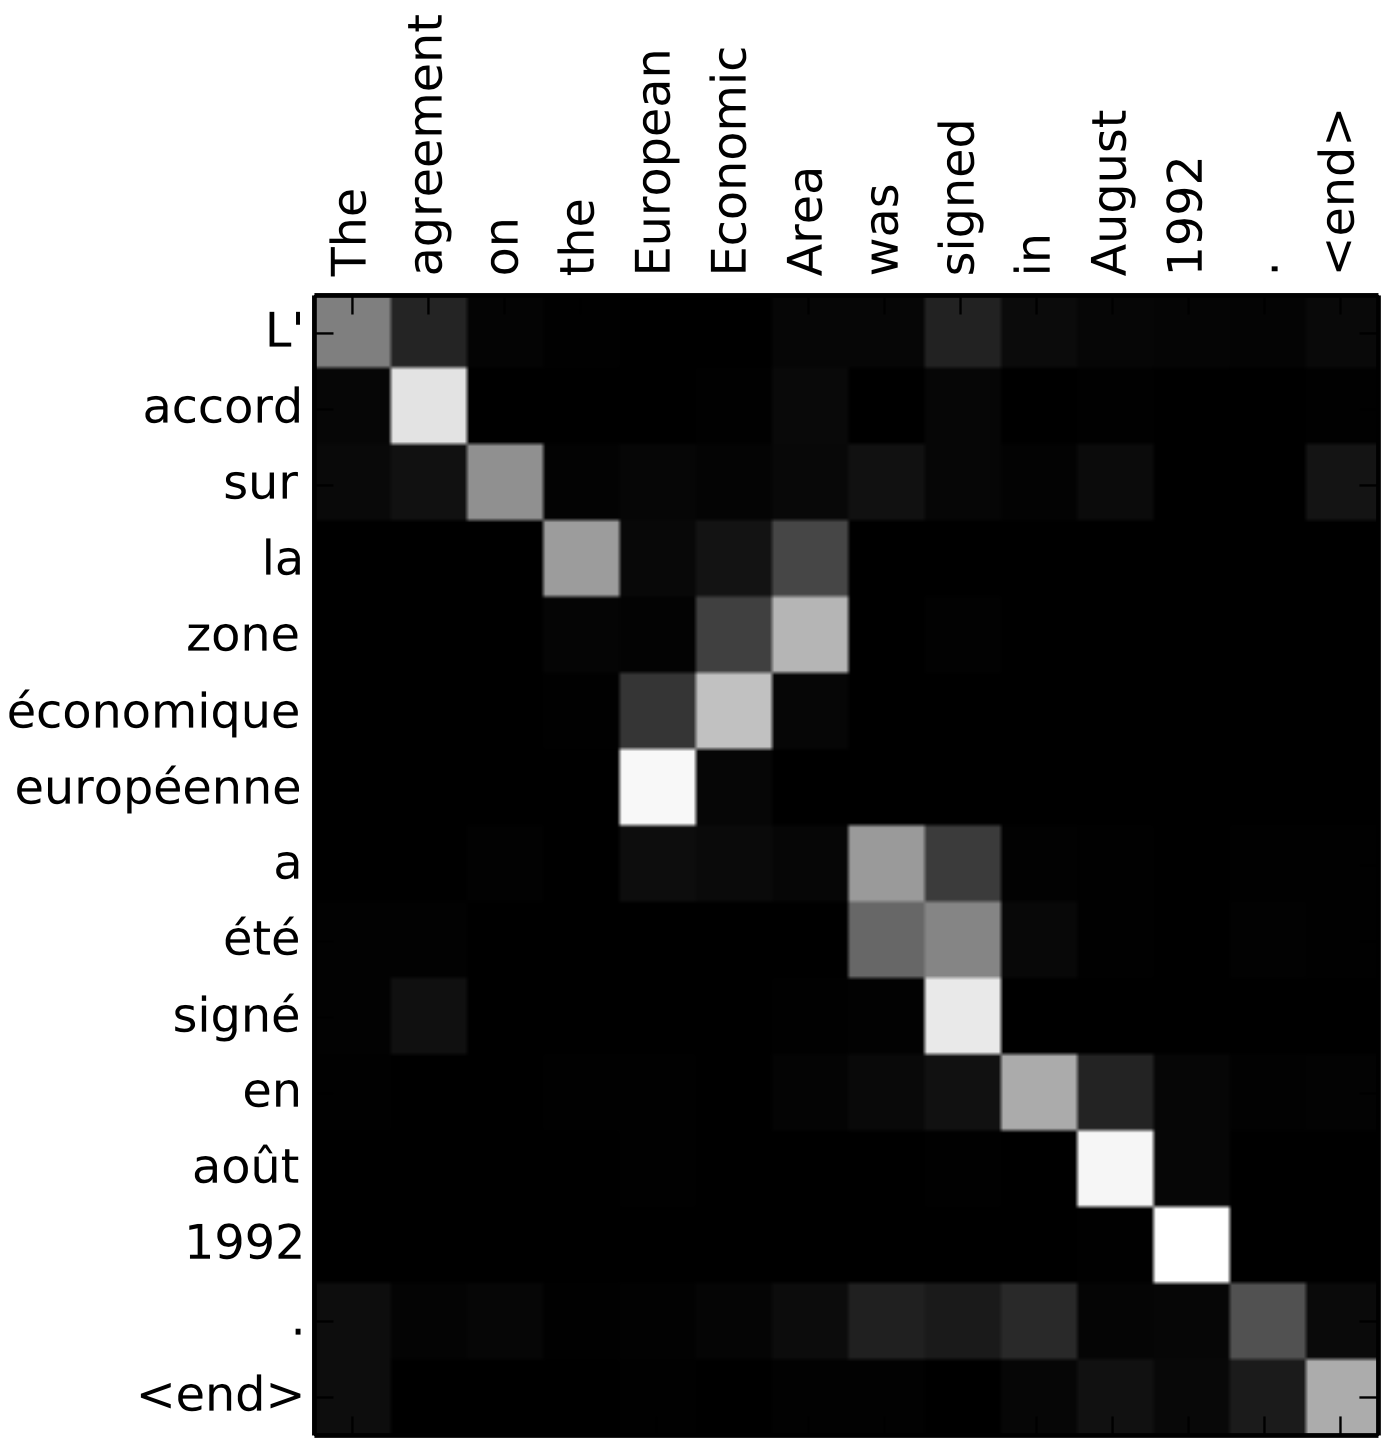
\includegraphics[scale=0.3]{2_production_mots_cles/attention_alignment.png}
    \caption{Exemple de visualisation des poids d'alignement du mécanisme d'attention entre une phrase en anglais et sa traduction en français. Chaque ligne montre la distribution des poids $\alpha_{t}$ ayant servis à générer le mot correspondant en français. Une case blanche indique un poids de 1, une case noire indique un poids de 0. Image extraite de \citet{bahdanau_neural_2014}.}
    \label{fig:attention_alignment}
\end{figure}

%Il faudra aussi porter attention à la syntaxe des deux langues
%Les poids d'attention peuvent être utilisés pour visualiser l'alignement entre les mots de la séquence d'entrée et ceux de la séquence de sortie.
%La figure~\ref{fig:attention_alignment} montre les poids d'alignement dans le cadre de la traduction automatique entre une phrase en anglais et sa traduction en français.

Le décodeur utilise l'état caché courant $h^d_t$ pour générer un mot, le mécanisme d'attention lui permet d'utiliser aussi tous les états cachés de l'encodeur $h^e$ pour mettre à jour l'état caché du décodeur $h^d_t$. Ce mécanisme est décrit dans l'équation~\ref{eq:attention}.
Dans le mécanisme d'attention, les états cachés $h^e$ sont pondérés en fonction de leur importance pour générer le mot $\hat{y}_t$.
Cette importance est établie grâce à une fonction d'alignement $a$ qui calcule une similarité entre l'état caché courant $h^d_t$ et ceux de l'encodeur $h^e$.
Les états cachés $h^e$ sont ainsi moyennés dans le vecteur de contexte $c_t$ utilisé pour mettre à jour l'état caché courant du décodeur $h^d_t$.

Dans l'équation \ref{eq:attention}: $[u;v]$ représente l'opération de concaténation des vecteurs $u$ et $v$; $a$ est une fonction d'alignement qui calcule la similarité entre un état caché de l'encodeur $h^e_t$ et du décodeur $h^d_t$; $\alpha$ représente les poids d'alignement entre les états cachés de l'encodeur $h^e$ et du décodeur $h^d$;  et $\textsc{Softmax}$ est une fonction qui normalise les valeurs d'un vecteur pour qu'il somme à 1.


\iffalse
    \begin{figure}
        \centering
        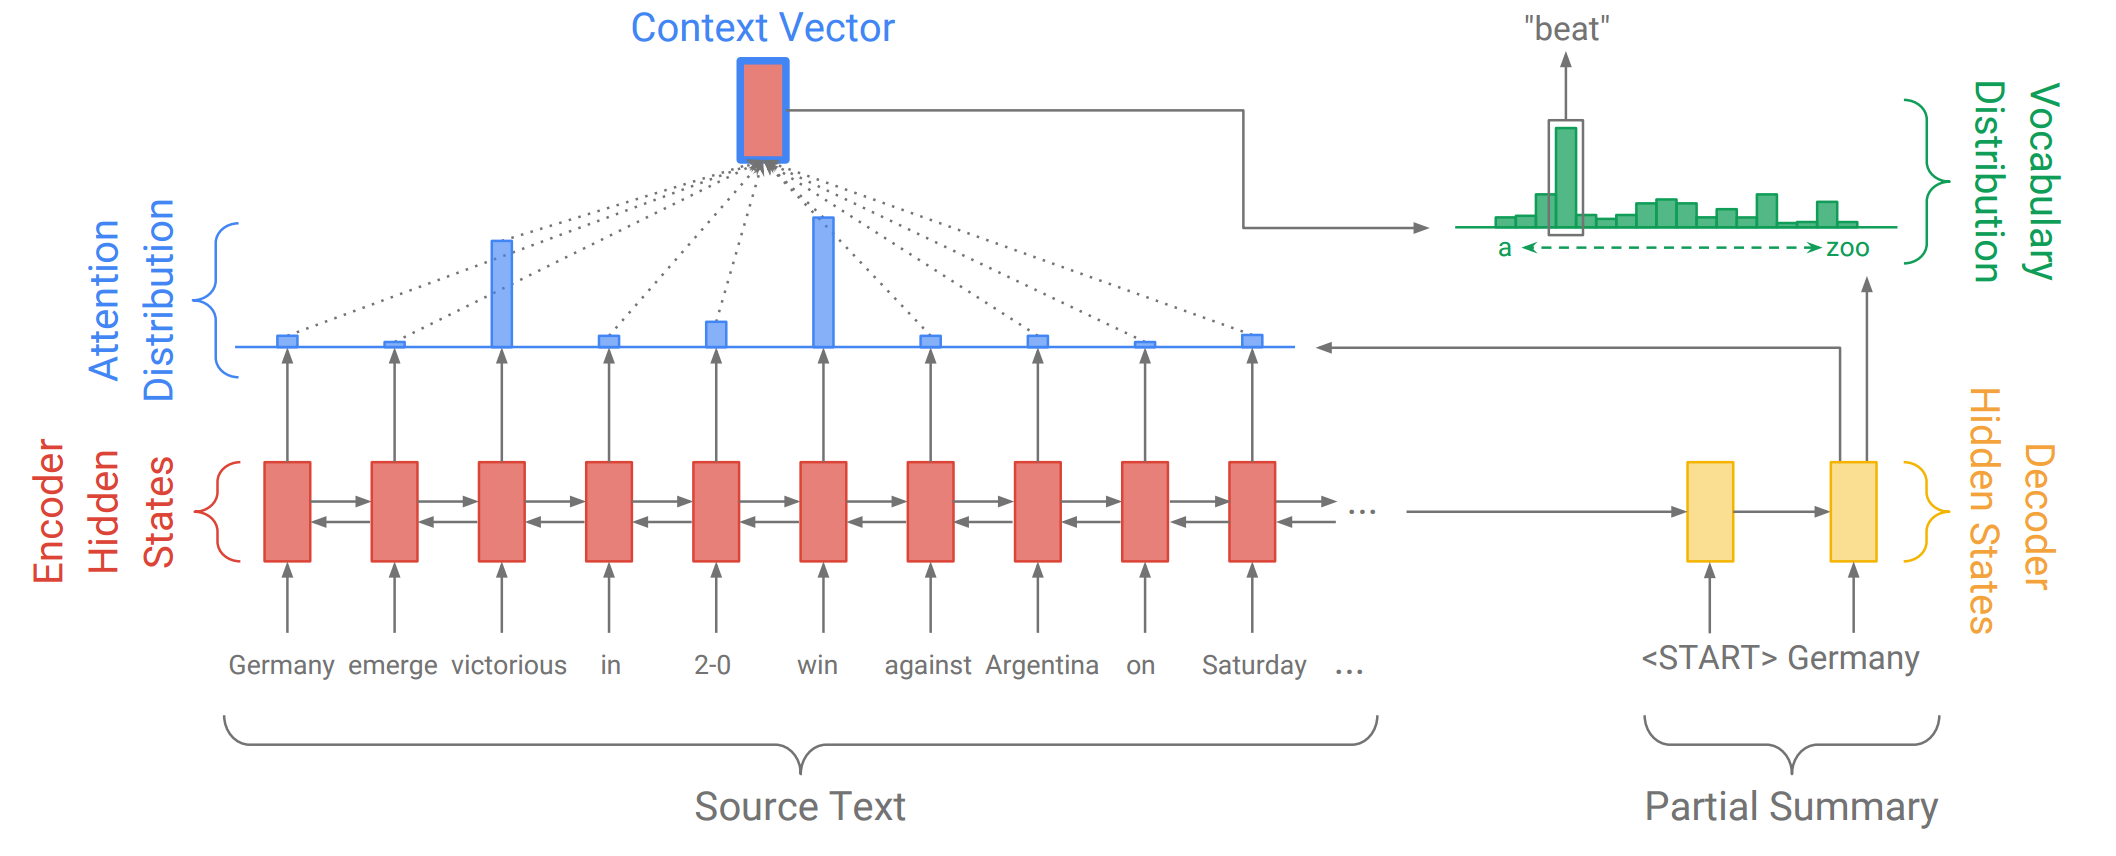
\includegraphics[width=\linewidth]{figures/see_seq2seq-attn.png}
        \caption{Schéma du mécanisme de copie présenté par \cite{see_get_2017}.}
        \label{fig:see_attention}
    \end{figure}
\fi

\begin{equation}\label{eq:attention}
  \begin{split}
    %\hat{Y}_t & = \sigma(b_v + W_v * h^d_t) \\
    p(y_t|y_{<t},x) & = \textsc{Softmax}(\sigma(W_v h^d_t)) \\[.3em]
    h^d_t & = \textsc{Rnn}(y_{t-1}, [h^d_{t-1};c_t]  \\[.3em]
    c_t & = \sum^{|h^e|}_{i=0} \alpha_{i,t} h^e_i \\
    \alpha_{t} & = \textsc{Softmax}(a(h^d_t, h^e)) \\
    %\textsc{Softmax}(x) & = \left[ \frac{x_i}{\sum^{|x|}_{i=0} x_i} , i \in |x| \right]
  \end{split}
\end{equation}

%Le concept d'attention a été présenté de deux manières différentes par \cite{bahdanau_neural_2014} et \cite{luong_effective_2015}.
%
%L'idée de l'attention présentée par~\cite{luong_effective_2015} est \emph{d'utiliser le vecteur de contexte pour prédire $y_t$}.
%
%\cite{bahdanau_neural_2014} présente un autre mécanisme d'attention dont l'idée est de calculer l'état caché du décodeur à l'aide d'un vecteur de contexte. Par rapport à un décodeur classique, seul le calcul de $h^d_t$ change.

\iffalse
    L'idée de l'attention présentée par~\cite{luong_effective_2015} est \emph{d'utiliser le vecteur de contexte pour prédire $y_t$}.
    
    Pour cela, un nouveau $\hat{h}^d_t$ est calculé en fonction d'un vecteur de contexte $c_t$ et de $h^d_t$ (calculé en fonction de $y_{t-1}$ et $h^d_{t-1}$). $c_t$ est la moyenne des $h^e$ pondérés par les scores d'alignement $\alpha$.
    
    Dans leur article, deux manières de calculer l'attention sont présentées: une attention globale et une attention locale.
    %
    Pour l'attention globale, le vecteur de contexte est la moyenne pondérée de toutes les représentations de l'encodeur.
    %
    Pour l'attention locale, le vecteur de contexte est la moyenne pondérée des représentations $h^e$ dans une fenêtre de taille $D$ autour de $h^e_{p_t}$.
    %
    $p_t$ est une valeur entre 0 et $|h^e|$ qui définit le centre de la fenêtre, et peut être calculé de différentes manières.\footnote{Pour plus de détails voir la section 3.2 de \cite{luong_effective_2015}}
    %$p_t$ étant $t$ (dans la traduction automatique on considère que le mot cible $y_t$ est aligné avec le mot source $x_{p_t}$), ou alors un réel entre 0 et $|h^e|$ calculé à l'aide 
    
    \begin{align}
        %y_t & = \sigma(W_v h^d_t) \\
        p(y_t | y_{<t}, x) & = \textsc{Softmax}(W_v \hat{h}^d_t) \\
        \hat{h}^d_t & = \sigma(W_c [c_t;h^d_t]) \\
        c_t & = \sum^{|h^e|}_{i=0} \alpha_{i,t} * h^e_i \\
        \alpha_{i,t} & = \textsc{Softmax}(a(h^e_i, h^d_t)) \\
        h^d_t & = \textsc{Rnn}(y_{t-1}, h^d_{t-1})
    \end{align}
    
    \cite{bahdanau_neural_2014} présente un autre mécanisme d'attention dont l'idée est de calculer l'état caché du décodeur à l'aide d'un vecteur de contexte. Par rapport à un décodeur classique, seul le calcul de $h^d_t$ change. Le calcul du vecteur de contexte est similaire à celui de ~\cite{luong_effective_2015}.
    
    \begin{align}
        p(y_t|y_{<t},x) & = \textsc{Softmax}(W_v h^d_t) \\
        h^d_t & = \textsc{Rnn}(y_{t-1}, [h^d_{t-1};c_t]  \\
        c_t & = \sum^{|h^e|}_{i=0} \alpha_{i,t} * h^e_i \\
        \alpha_{i,t} & = \textsc{Softmax}(a(h^e_i, h^d_t))
    \end{align}
    
    Il existe différentes fonctions d'alignement:
    
    bahdanau $a(h^e_i, h^d_t) = v_a \text{tanh}(W_a h^d_t + U_a h^e_i)$
    
    dot $a(h^e_i, h^d_t) = h^e_i h^d_t$
    
    general $a(h^e_i, h^d_t) = h^e_i W_a h^d_t$
    
    concat $a(h^e_i, h^d_t) = W_a [h^e_i;h^d_t]$
\fi

\subsubsection{Mécanisme de copie}
\label{sub:copy_mecanism}

Le mécanisme de copie~\cite{see_get_2017,gu_incorporating_2016} provient des tâches de traduction automatique et de résumé automatique. Il a pour but de produire des mots peu fréquents ou hors du vocabulaire de sortie.
En effet, les modèles neuronaux qui génèrent du texte choisissent les mots dans un vocabulaire de sortie comportant généralement \num{50 000} mots.
Dans les tâches sus-citées, les mots peu fréquents qui ne font pas partie du vocabulaire de sortie, comme les entités nommées ou les transfuges, doivent pourtant apparaître dans la séquence de sortie.
%Le mécanisme de copie ~\cite{see_get_2017,gu_incorporating_2016} pallie ce problème en permettant au décodeur de générer un mot du vocabulaire de sortie ou bien de copier un mot du document.
Deux mécanismes de copie ont été proposés par \citet{see_get_2017} et \citet{gu_incorporating_2016}; les deux étant similaires, nous présentons ici le premier car plus simple. Il est décrit dans l'équation~\ref{eq:copy_mecanism}.

% exemple
%Le mécanisme d'attention a été utilisé comme post-traitement pour remplacer les mots inconnus de la sortie par les mots de l'entrée alignés par le mécanisme d'attention. Ceci permettant de traiter les entités nommées peu fréquentes ou les transfuges.
%
%Le mécanisme de copie vient automatiser ce processus en permettant au modèle de générer un mot du vocabulaire ou de copier un mot du document.

%, tous deux inspirés des réseaux de pointeurs~\cite{vinyals_pointer_2015} qui génèrent une séquence de pointeurs vers la séquence d'entrée.
Ce mécanisme utilise le vocabulaire de la séquence d'entrée $\mathcal{X}$ (particulier à chaque document) en plus du vocabulaire de sortie $\mathcal{V}$.
Pour produire un mot, une distribution de probabilité sur le vocabulaire  $P_{vocab}(y_{t})$ est calculée comme précédemment par le décodeur (cf. section~\ref{sub:decoding}) et les poids du mécanisme d'attention $\alpha$ (cf. section~\ref{sub:attention_mecanism}) sont utilisés pour estimer la probabilité de copie de chaque mot du document.
Les poids d'attention $\alpha$ des mots qui apparaissent plusieurs fois dans l'entrée $x$ sont sommés $\sum_{j,x_j=y_{t,i}} \alpha^t_j$.
Ainsi, un mot peut être généré à partir du vocabulaire de sortie $\mathcal{V}$ ou copié à partir du vocabulaire du document $\mathcal{X}$.
Les probabilités de copie et de génération d'un même mot, qui appartient au document et au vocabulaire, sont sommées.
Dans l'équation~\ref{eq:copy_mecanism}: $h^d_t$, $c_t$ et $\alpha^t_j$ proviennent du mécanisme d'attention (cf. équation~\ref{eq:attention}); $p_{gen}$ est un curseur permettant au modèle de privilégier la copie ou la génération et $P_{vocab}(y_t)$ est une distribution de probabilité sur le vocabulaire de sortie $\mathcal{V}$.

%Les probabilités de génération et de copie sont combinés pour donner une distribution de probabilités sur $\mathcal{X} \cup \mathcal{V}$.

\begin{equation}\label{eq:copy_mecanism}
  \begin{split}
    p(y_{t,i}|y_{<t},x) & = p_{gen} P_{vocab}(y_{t,i}) + (1 - p_{gen}) \sum_{j,x_j=y_{t,i}} \alpha^t_j \\
    p_{gen} & = \sigma(W_h h^d_t + W_c c_t + W_y y_{t-1}) \\
    P_{vocab}(y_{t}) & = \textsc{Softmax}(\sigma(W_v h^d_t))
  \end{split}
\end{equation}

%ou les poids d'un mécanisme d'attention supplémentaire, utilisé seulement pour calculer le score de copie, pour~\cite{gu_incorporating_2016}

\iffalse
    %\cite{gu_incorporating_2016}, création d'un vocabulaire spécifique a chaque instance, composé de $\mathcal{V}$ le vocabulaire normal et $\mathcal{X}$ le vocabulaire des mots de l'entrée.
    %
    %Ça change le calcul de $y_t$ par rapport au mécanisme d'attention.
    %
    %On défini les vecteurs $\psi_g \in \mathds{R}^|\mathcal{V}|$ et $\psi_c \in \mathds{R}^|\mathcal{X}|$ qui contiennent respectivement les score de copie et de génération.
    
    % attentive read = les poids de l'attention
    % selective read = les poids de l'"attention" du mécanisme de copie
    
    \begin{align}
        y_t & = \textsc{Softmax}(e^{P_{gen}} +e^{P_{copy}}) \\
        P_{gen} & = W_v h^d_t \\
        P_{copy} & = \left[ \sum^{|h^e|}_{j=0, x_j=x_i} \sigma(h^e_j W_c) h^d_t | x_i \in \mathcal{X} \right] \\
        h^d_t & = RNN([y_{t-1};cc_t)],h^d_{t-1}) \\
        cc_t & = \sum^{|h^e|}_{i=1} aa_{t,i} h^e_t \\
        aa_{t,i} & = \textsc{Softmax}()
    \end{align}
    
    %\cite{see_get_2017} reprend le mécanisme d'attention de \cite{luong_effective_2015} et modifie le calcul de $y_t$ en ajoutant une probabilité de copie et un curseur privilégiant la copie ou la génération.
    
    \begin{align}
        p(y_{t,i}) = p_{gen} P_{vocab}(y_{t,i}) + (1 - p_{gen}) \sum_{j,x_j=y_{t,i}} \alpha^t_j \\
        p_{gen} = \sigma(W_c c_t + W_h h^d_t + W_y y_{t-1})
    \end{align}
\fi

% Multitache
% Conditional Random Field
% Reinforcement Learning : adaptative reward


\section{Méthodes de bout-en-bout}
\label{methodes-de-bout-en-bout}

\todo{Ajouter des schéma pour mieux comprendre les méthodes.}

Dans cette section nous présentons un état de l'art des méthodes de bout-en-bout.
Ces méthodes, contrairement aux méthodes en chaîne de traitement (cf. section~\ref{sec:methode-en-chaine-de-traitement}), prennent en entrée un document et laissent le soin au modèle d'en extraire les caractéristiques pour retourner un ensemble de mots-clés sans étapes intermédiaires ni définition manuelle de ces caractéristiques.
Parmi les méthodes proposées dans la littérature, nous distinguons les méthodes génératives, qui peuvent produire des mots-clés présents et des mots-clés absents, des méthodes extractives, limitées aux mots-clés présents.

Jusqu'à présent, toutes les méthodes de bout-en-bout qui ont été proposées sont supervisées et reposent sur des réseaux de neurones (cf. section~\ref{sub:neural_network}) qui nécessitent de grandes quantités de données annotées pour être entraînées.
%
Le développement de ces méthodes démarre avec l'introduction du jeu de données KP20k et de la méthode générative CopyRNN par \citet{meng_deep_2017}.
Le jeu de données KP20k, qui comporte $\simeq$\num{550000} documents, comble un manque.
En effet, seuls de petits jeux de données (de l'ordre du millier de documents) étaient jusqu'alors disponibles.
Ce travail a ainsi lancé une nouvelle direction de recherche sur les méthodes génératives de production de mot-clés.

\begin{figure}
    \centering
    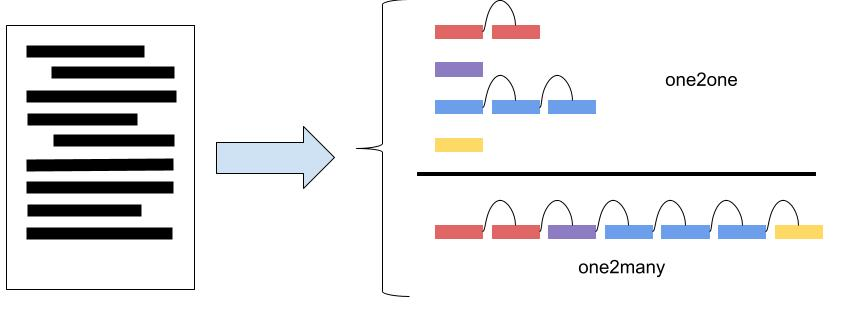
\includegraphics[scale=0.4]{2_production_mots_cles/Decoding strategies.jpg}
    \caption{Représentation schématique des stratégies de décodage \emph{one2one} et \emph{one2many}.}
    \label{fig:decoding_strategies}
\end{figure}
\todo{Refaire en tikz}

Dans cet état de l'art, nous présentons tout d'abord les méthodes automatiques de génération de mots-clés de bout-en-bout, qui sont au c\oe{}ur de ce travail de thèse.
Nous présentons ces méthodes de génération en deux parties: premièrement, les méthodes qui générent les mots-clés un à un (\emph{one2one}), et deuxièmement, celles qui génèrent des séquences de mots-clés (\emph{one2many}). Ces deux types de génération sont schématisés dans la figure~\ref{fig:decoding_strategies}.
Nous présentons ensuite les méthodes extractives de bout-en-bout, c'est-à-dire celles qui se limitent aux seuls mots-clés présents.

\subsection{Génération de mots-clés}
\label{sub:generation_de_mots_cles}

Les méthodes génératives, introduites par \citet{meng_deep_2017}, ont pour objectif de pallier deux faiblesses qui concernent la majorité des méthodes extractives présentées précédemment: l'impossibilité de produire des mots-clés absents ainsi que la faible prise en compte de la sémantique.
Le paradigme encodeur-décodeur sur lequel les méthodes génératives sont fondées permet d'encoder la sémantique du document.
Ainsi, les mots-clés produits sont le fruit d'une \say{compréhension} du document, contrairement aux méthodes en chaîne de traitement qui s'intéressent à l'\say{importance} des mots dans le document indépendamment de leur sens.
%
Ces méthodes génératives rendent possible la production de mots-clés absents grâce à la manière dont le décodeur génère la séquence de sortie.
Ce processus s'effectue en choisissant, à chaque étape de décodage, un mot à partir d'un vocabulaire de sortie qui est plus grand et différent du vocabulaire du document.
Ces méthodes génératives apprennent à générer des mots-clés un par un (génération \emph{one2one}, voir figure~\ref{fig:decoding_strategies}), c'est-à-dire que chaque document $X$ et son ensemble de mot-clés $Y$ de taille $N$ forment un couple $(X, \{Y_0, ..., Y_N\})$, décomposé en autant d'exemples d'entraînement que de mots-clés, $(X, Y_0), ... , (X, Y_N)$.

%\paragraph{Définitions}
%\todo{Il faudrait définir avant les principaux modèles: one2one, séquence avant de les définir formellement; Fait ausi des dessins}
%$x$ et $y$ représentent des mots, $p$ des mots-clés. Étant donné un ensemble de données $D = {(x^i,p^i), i \in 1...N}$ de taille $N$, un exemple est composé d'un document $x^i$ et d'un ensemble de mots-clés $p^i = {p^i_j, j \in 1...M^i}$ de taille $M^i$. Les documents et les mots-clés sont composés de mots $[x^i_k, k \in 1...N^i]$ et $[y^i_j]$ est composé d'un document composé d'une séquence de mots $x^i = (x^i_1, ..., x^i_{N^i})$ de longueur $N^i$ et d'un ensemble de mots-clés $p^i$ de taille $M^i$ avec $p^i = (p^i_1, ..., p^i_{M^i})$, où chaque mot-clé est une séquence de mots de taille $M^{i,j}$ avec $p^{i,j} = (y^{i,j}_1, ..., y^{i,j}_{M^{i,j}})$. Dans le cadre des modèles one2one, un couple document -- mots-clés est découpé en $M^i$ différents couples $(x^i, p^{i,1}), ..., (x^i, p^{i, M^i})$. 
%Pour les modèles en séquences, les mots-clés sont concaténés de sorte à former une unique séquence $(x^i, y^{i,1}_1 \lozenge ... \lozenge y^{i,1}_{M^{i,j}} \lozenge \text{SEP} \lozenge y^{i,2}_1 \lozenge ... \lozenge y^{i,M^i}_{M^{i,j}})$.

La méthode pionnière de génération automatique de mots-clés appliquée aux documents scientifiques est CopyRNN~\cite{meng_deep_2017}.
%
L'architecture neuronale de cette méthode s'inspire du processus d'annotation humain qui consiste à lire le document pour le comprendre dans son entièreté puis à le résumer grâce à des mots-clés.
%Aussi, les humains peuvent facilement s'abstraire du texte et faire appel à leurs connaissances pour produire des mots-clés qui n'apparaissent pas dans le texte.
Pour reproduire ce processus, CopyRNN utilise le paradigme encodeur-décodeur, que nous avons présenté dans la section~\ref{sub:paradigme_encodeur_decodeur}, pour encoder un document et le décoder ensuite en un mot-clé. % Ainsi un réseau de neurones récurrent encode le document dans un vecteur de pensée, puis un autre décode, génère, ce vecteur de pensée en un mot-clé.
Pour améliorer les performances des modèles encodeur-décodeur, il est commun d'utiliser un mécanisme d'attention (voir section~\ref{sub:attention_mecanism}).
Ce mécanisme permet au modèle de porter attention à certaines parties du document lors de la génération d'un mot.
%
Un mécanisme de copie est aussi ajouté au modèle pour lui permettre de générer des mots peu fréquents (voir section~\ref{sub:copy_mecanism}).
Ce mécanisme de copie modifie le décodage en permettant de générer un mot à partir du vocabulaire de sortie ou bien à partir du document.\\
%
Cette méthode obtient des performances bien plus élevées que les précédentes méthodes extractives. Les performances de CopyRNN sont de l'ordre de 30 points de \fmesure{} pour les mots-clés présents tandis que les performances des méthodes extractives sont généralement en dessous de 20 points de \fmesure{}.
Les mots-clés absents, qui ne pouvaient jusque-là pas être produits, correspondent peu à la référence: parmi les 50 meilleurs mots-clés absents un seul apparaît dans la référence.


%La communauté scientifique présente de nouvelles méthodes basées sur CopyRNN et tente de l'améliorer.
% les méthodes essaient de résoudre les problèmes identifiés
%Les méthodes présentées augmentent toujours les performances de génération des mots-clés présents et absents.

Certaines méthodes proposées essaient d'améliorer l'encodage du document.
\citet{chen_title-guided_2019}, par exemple, constate que les mots-clés ne sont pas uniformément distribués dans les documents.
En particulier \npercent{60} des mots-clés de référence ont au moins un mot en commun avec le titre du document.
Pour prendre cela en compte, ils proposent TGNet (Title Guided Network), qui étend CopyRNN en introduisant un nouvel encodeur spécifique au titre, en plus de l'encodeur du document.
Cet encodage du titre permet de donner un poids supplémentaire à l'information qu'il contient.
Ces deux représentations (du titre et du document) sont ensuite combinées puis fournies au décodeur.
Cette méthode améliore nettement les performances de génération des mots-clés présents et absents par rapport à CopyRNN (+\npercent{5} sur KP20k).
% Ils ne regardent que la F-mesure présent/absent rien d'autre

La redondance dans les ensembles de mots-clés produits est un problème récurrent dans les méthodes de production de mots-clés.
En effet, \citet{hasan_automatic_2014} montrent que 8 à \npercent{12} des erreurs des méthodes sont liées à la redondance des mots-clés.
Ainsi, les méthodes en chaîne de traitement mettent en place des stratégies, notamment lors de la sélection du sous-ensemble de mots-clés, pour limiter cette redondance (voir section~\ref{choisir-le-sous-ensemble}).
Dans cette ligne de recherche, \citet{zhao_incorporating_2019} remarquent les méthodes de bout-en-bout ne sont pas exemptes de ce problème, ils s'intéressent ainsi au chevauchement entre les mots-clés générés et ceux de référence.
Par exemple, \npercent{23.98} des mots-clés unigrammes générés par CopyRNN font partie d'un mot-clé de référence, et \npercent{47.15} des mots-clés 4-grammes générés par CopyRNN contiennent un mot-clé de référence.
Dans l'optique de limiter ces chevauchement, ils présentent le modèle ParaNet$_T$+CoAtt qui entraîne le modèle, à générer à la fois les mots-clés et leurs étiquettes morphosyntaxiques, ainsi la syntaxe des mots-clés générés sera similaire à celle des mots-clés de référence.
Pour cela ils ajoutent au modèle CopyRNN un encodeur, pour les étiquettes morphosyntaxiques des mots du document, ainsi qu'un décodeur, pour celles du mot-clé.\footnote{Les étiquettes morphosyntaxiques du document et des mots-clés proviennent de l'outils Stanford CoreNLP.}
Les informations des deux décodeurs sont ensuite combinées et utilisées pour générer les mots-clés et leurs étiquettes morphosyntaxiques.
%Grâce à cette méthode, les mots-clés générés chevauchent moins les mots-clés de référence; par exemple le pourcentage de mot-clés 4-grammes contenant un mot-clé de référence a baissé de \npercent{10}.

\begin{figure}
    \centering
    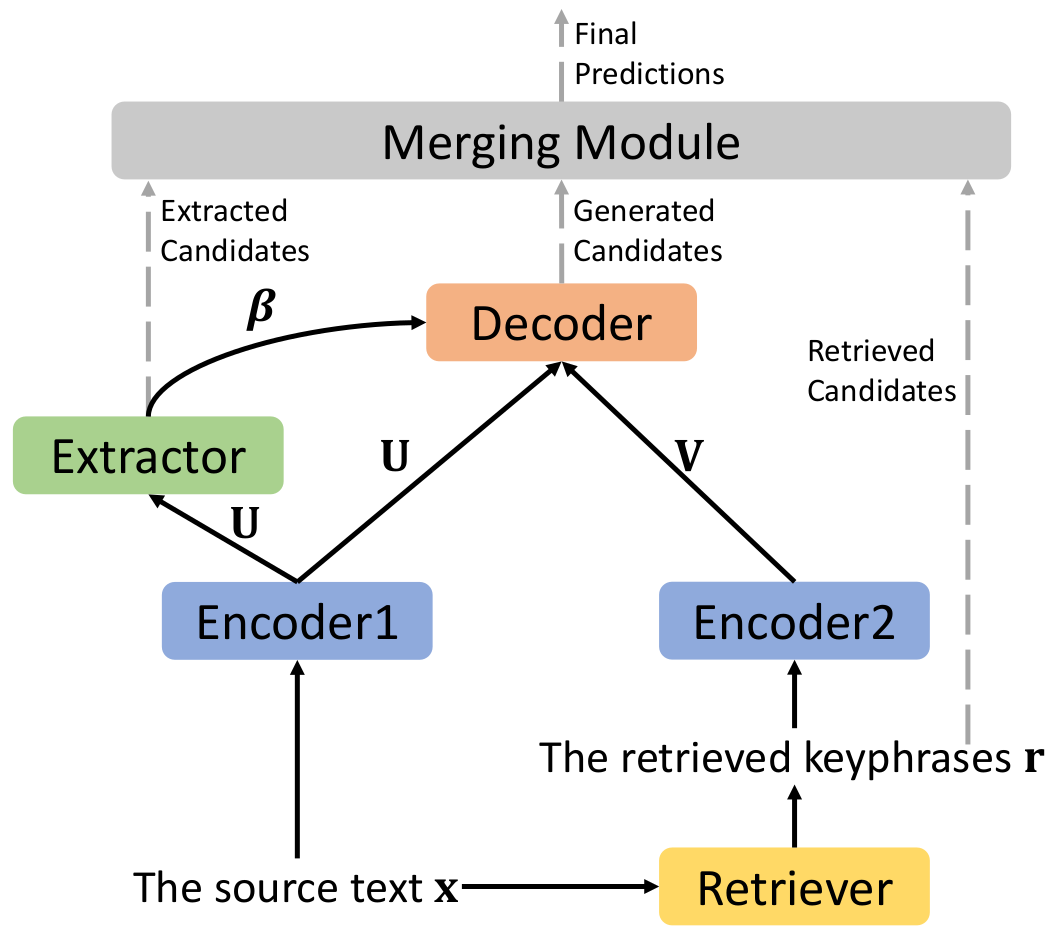
\includegraphics[scale=0.2]{2_production_mots_cles/kg_ke_kr_m.png}
    \caption{Représentation schématique de l'architecture de la méthode KG-KE-KR-M. Image extraite de~\citet{chen_integrated_2019}.}
    \label{fig:schema_kgkekrm}
\end{figure}

%Le processus manuel d'annotation en mots-clés est composé de plusieurs étapes: la lecture du document, l'extraction des mots-clés dans le document puis l'attribution de mots-clés absents du document et enfin la combinaison des mots-clés provenant de ces deux processus d'annotation.
Dans l'optique de reproduire l'annotation humaine, \citet{chen_integrated_2019} propose la méthode KG-KE-KR-M qui produit un ensemble de mots-clés en combinant différentes méthodes: génération de mots-clés, extraction de mots-clés, récupération de mots-clés (voir figure~\ref{fig:schema_kgkekrm}).
%Ces différentes méthodes sont entraînées de bout-en-bout puis les mots-clés de chaque méthode sont pondérés grâce à un classifieur.
%
Dans un premier temps, cette méthode récupère les mots-clés de référence des $K$ documents d'entraînement les plus proches du document traité (grâce à la distance de Jaccard).
Ces mots-clés \emph{récupérés} sont concaténés puis encodés. Ils serviront à conditionner la génération de mots-clés.
Dans un second temps, des mots-clés sont \emph{extraits} du document en classifiant chaque mot comme mot-clé ou non mot-clé.
%Cette classification s'effectue grâce aux états cachés du document encodé.
Ensuite, des mots-clés sont \emph{générés} à partir du document ainsi que des mots-clés récupérés et des mots-clés extraits.
Enfin, les mots-clés récupérés, extraits et générés sont pondérés grâce à un classifieur.
Cette méthode à la particularité de combiner les méthodes en chaîne de traitement (sélection de candidats puis pondération) et les méthodes de bout-en-bout (apprentissage conjoint de la génération et de l'extraction).
Malgré la grande diversité dans les techniques de production de mots-clés candidats, les performances ne sont pas significativement supérieures à CopyRNN. Cette méthode produit néanmoins plus de mots-clés absents de référence que CopyRNN.

La méthode CorrRNN~\cite{chen_keyphrase_2018} considère que les mots-clés doivent couvrir l'ensemble des sujets du document et être divers, c'est-à-dire que chaque mot-clé doit concerner un sujet différent.
Cette méthode étend CopyRNN en y ajoutant un mécanisme de couverture et un mécanisme de revue.
Le mécanisme de couverture encourage le modèle à porter attention aux différentes parties du document.
Il conserve et accumule les scores d'attention des mots du document à chaque étape de décodage, et il est inclus dans le calcul du mécanisme d'attention.
Ensuite, le mécanisme de revue est essentiellement un mécanisme d'attention sur les mots générés.
Son objectif est d'identifier les sujets déjà couverts par les mots-clés générés et ainsi de générer des mots-clés qui concernent des sujets non traités.
Cette méthode est la première à prendre en compte les mots-clés déjà générés dans le processus de génération, pour cela la phase d'entraînement est modifiée.
Au lieu de rétro-propager le gradient après chaque mot-clé de référence, la phase de rétro-propagation n'est effectuée qu'une fois tous les mots-clés de référence du document traités.
%Chaque mot-clé est généré en utilisant les mécanismes de couverture et de redondance, qui prennent en compte les mots-clés déjà générés; le gradient est ensuite calculé grâce à l'erreur de chaque mot-clé; et enfin, rétro-propagé.
%Cette méthode améliore les performance de production de mots-clés présent par rapport à CopyRNN, mais l'article ne présentant pas ses résultats sur le jeu de données de référence KP20k et utilisant des métriques peu utilisés dans les autres travaux la comparaison est limitée.

\subsection{Génération de séquences de mots-clés}% (\textsc{One2Seq})}
%\subsection{Génération en séquence}
\label{sub:generation_de_sequences_de_mots_cles}

%Nous avons présenté dans la section précédente, des méthodes génératives qui apprennent à générer un mot-clé par document.
Nous présentons dans cette section des méthodes qui apprennent à générer des séquences de mots-clés (génération \emph{one2many}, voir figure~\ref{fig:decoding_strategies}). C'est-à-dire que chaque exemple d'entraînement est composé d'un document et de la concaténation des mots-clés de référence en une unique séquence dans laquelle ils sont séparés par un symbole de séparation. Par exemple, l'ensemble de mots-clés $\{$ Classe , Fichier log , Agrégat $\}$ sera transformé en \say{Classe \texttt{SEP} Fichier log \texttt{SEP} Agrégat \texttt{FIN}}.
%Le développement des méthodes utilisant la génération \emph{one2many} part du constat que la génération \emph{one2one} ne permet pas de prendre en compte les mots-clés déjà générés et que les ensembles de mots-clés sont souvent redondants~\cite{hasan_automatic_2014}.
Le développement des méthodes génératives \emph{one2many} part du constat que les ensembles de mots-clés produits sont souvent redondants~\cite{hasan_automatic_2014} et que la génération \emph{one2one} ne permet pas de pallier ce problème.
En effet, les méthodes \emph{one2many} font l'hypothèse qu'avec la génération en séquence, le modèle ayant accès aux mots-clés déjà générés, il ne générera pas de mots-clés redondants.
%
Cette méthode de génération permet au modèle de générer le même nombre de mots-clés que la référence, en effet, il apprend en même temps qu'à générer les mots-clés, à placer les séparateurs de mots-clés et le symbole de fin.
Ainsi, ces méthodes peuvent générer des mots-clés selon deux stratégies~\cite{yuan_one_2020}: l'\textbf{inférence exhaustive} qui utilise l'algorithme de recherche en faisceau pour sur-générer des mots-clés et ainsi en obtenir un nombre fixe pour chaque document, c'est la stratégie employée par les méthodes génératives \emph{one2one}; et l'\textbf{inférence auto-régulée} (\foreign{self-terminating}) dans laquelle le décodage s'arrête lors de la génération du symbole de fin, cette stratégie permet au modèle de produire un nombre pertinent de mots-clés pour le document.
La seconde stratégie de décodage permet donc de s'affranchir du choix arbitraire du nombre de mots-clés $n$ à produire (voir section~\ref{choisir-le-sous-ensemble}).

Pour entraîner ces modèles, les mots-clés sont concaténés, mais ce processus n'est pas trivial.
En effet, l'ordre dans lequel les mots-clés sont concaténés influence les performances des modèles.
L'étude de \citet{meng_empirical_2021} compare différentes manières d'ordonner les mots-clés, telles que: \emph{No-Sort} qui laisse l'ordre par défaut; \emph{Alpha} qui trie par ordre alphabétique; \emph{Pres-Abs} qui place les mots-clés présents avant les mots-clés absents. L'étude montre que c'est l'ordre \emph{Pres-Abs} qui donne les meilleures performances.

La première méthode à générer des séquences de mots-clés est catSeqD~\cite{yuan_one_2020,yuan_generating_2018}.
L'objectif de cette méthode, similaire à CorrRNN, est d'augmenter la diversité des mots-clés générés.
%
Pour cela, le modèle CopyRNN, utilisé comme base, est augmenté d'un mécanisme de couverture sémantique et de régularisation orthogonale pour former le modèle catSeqD.
%
Le mécanisme de \emph{couverture sémantique} repose sur l'hypothèse que l'ensemble de mots-clés de référence et le document encodent la même information.
Ainsi, un nouvel encodeur est entraîné à encoder les mots-clés et à produire la même représentation que pour le document.
Il encode la séquence au fur et à mesure de sa génération et l'état cachés qui en résulte conditionne la prédiction du mot suivant, cela contraint les mots-clés générés à être proche sémantiquement du document.
%
Ensuite, les auteurs constatent que les mots générés après les séparateurs de mots-clés sont souvent similaires.
Le mécanisme de \emph{régularisation orthogonale} pallie ce problème en diversifiant explicitement les représentations des séparateurs, en pénalisant, dans la fonction de coût, ces représentations si elles ne sont pas orthogonales.

\todo{Refaire en Tikz}
\begin{figure}
    \centering
    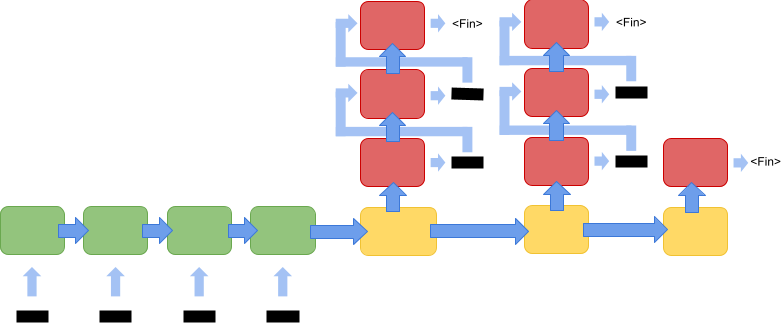
\includegraphics[scale=0.5]{2_production_mots_cles/exhird.png}
    \caption{Représentation schématique du décodage hiérarchique de la méthode ExHirD. L'encodeur du document est représenté en vert, le décodeur de concept en jaune et le décodeur de mots-clés en rouge.}
    \label{fig:schema_exhird}
\end{figure}

Dans le but de mieux modéliser les ensembles de mots-clés, \citet{chen_exclusive_2020} s'intéressent à la structure hiérarchique des ensembles de mots-clés.
En effet, les méthodes de génération de séquences de mots-clés identifient les mots-clés grâce à des marqueurs générés par le modèle. Cette séquentialité ne permet pas de représenter la hiérarchie entre les mots-clés et les mots qui les composent.
Ces travaux se rapprochent de \citet{yuan_generating_2018} qui essaient de rompre la séquentialité en modifiant la représentation des séparateurs de mots-clés avec le mécanisme de régularisation orthogonale.
Ainsi, ils présentent la méthode ExHirD~\cite{chen_exclusive_2020} dans laquelle le décodeur de l'architecture de CopyRNN est remplacé par un décodeur hiérarchique (voir figure~\ref{fig:schema_exhird}) qui génère les mots-clés en deux temps: d'abord l'identification des concepts, ensuite la génération de leur représentation textuelle.
Ce décodeur hiérarchique comprend un premier décodeur qui produit une représentation dense d'un concept, puis un second décodeur qui va générer une séquence de mots à partir de cette représentation dense pour instancier le concept en un mot-clé.
La génération des mots utilise deux mécanismes d'attention sur les documents d'entrée: l'un est conditionné par la représentation dense du concept; l'autre, standard, est conditionné par le mot précédent.
Ainsi, ce décodeur hiérarchique permet de modéliser explicitement les concepts importants du document et les mots qui les décrivent.
%
L'évaluation de cette méthode montre néanmoins un faible gain de performance, de l'ordre d'un point de F@5, pour les mots-clés présents et absents.
%
Ces travaux s'attellent aussi au problème de redondance des mots-clés et proposent un mécanisme de décodage exclusif pour tenter de le résoudre.
Ce mécanisme, simple dans son idée, interdit au modèle de générer deux mots-clés commençant par le même mot.
En effet, les mots-clés comportent le plus souvent entre 1 et 4 mots (voir section~\ref{sub:nature_linguistique}), ainsi le premier mot affecte grandement les suivants.
Ce mécanisme n'est pas limité à la méthode ExHirD; il peut être adapté aux différents types de décodage ou être utilisé en post-traitement.
Son évaluation montre qu'il fait significativement baisser le nombre de mots-clés dupliqués sans faire baisser les scores de F@5.

Les méthodes génératives \emph{one2many} apprennent à déterminer le nombre de mots-clés à produire mais en génèrent trop peu: catSeqD génère en moyenne 4,3 mots-clés par document alors que la référence en est composée de 5,3 en moyenne.
Les travaux de \citet{chan_neural_2019} s'intéressent à encourager les modèles à générer plus de mots-clés, en les entraînant à optimiser le rappel et la \fmesure{}.
Or ces métriques ne peuvent être utilisées comme fonction de coût dans l'algorithme de descente de gradient, car elles ne sont pas dérivables.
Pour résoudre ce problème, les auteurs proposent d'utiliser l'apprentissage par renforcement pour affiner\footnote{\foreign{To fine-tune} en anglais.} des modèles déjà entraînés.
%
Dans l'apprentissage par renforcement~\cite{williams_simple_1992}, un agent produit une série d'actions en suivant une politique (ici la génération de mots grâce à un modèle génératif), puis est récompensé pour chacune des actions.
%Dans l'apprentissage par renforcement~\cite{williams_simple_1992}, un agent produit une série d'actions en suivant une politique puis il est récompensé pour chaque action.
%Dans notre cas, une action consiste à générer un mot, la politique permettant de choisir le mot est un modèle génératif, et la récompense est le rappel ou la f-mesure.
L'algorithme d'apprentissage par renforcement optimise ainsi les poids du modèle (met à jour la politique) en fonction de la récompense.
%
Dans la méthode proposée, la récompense s'adapte selon le nombre de mots-clés générés: s'il est trop faible, la récompense sera le rappel pour encourager le modèle à générer plus de mots-clés; à l'inverse s'il est trop grand, la récompense sera la \fmesure{}, pour encourager le modèle à générer seulement de bons mots-clés.
%
De plus, les mots-clés présents et absents sont récompensés séparément pour favoriser la génération des mots-clés absents.

%CDKGen~\cite{diao_keyphrase_2020} (use close docs to encode, transformers)
%SenseNet~\cite{luo_sensenet_2020} (??)

Les travaux, concernant les méthodes neuronales, présentés jusqu'à présent considèrent que la quantité de données disponibles est suffisante.
Nous verrons dans le chapitre~\ref{chap:framework} que les sources de données contenant des documents annotés en mots-clés sont peu nombreuses malgré la large disponibilité de documents scientifiques en ligne.
Ainsi, les travaux de \citet{ye_semi-supervised_2018} se placent dans un cadre où la quantité de documents annotés est limitée.
%
Pour cela, les auteurs proposent deux méthodes qui tirent parti de la masse de documents non annotés pour la génération de mots-clés.
%
La première méthode consiste à utiliser des documents non annotés en mots-clés dans le cadre d'apprentissage multitâche.
Un réseau de neurones encodeur-décodeur est entraîné, pour les documents annotés, à générer des séquences de mots-clés et, pour les documents non annotés, à générer le titre du document. Dans le modèle, deux décodeurs différents sont utilisés pour chacune des tâches mais l'encodeur est partagé.
%
La seconde méthode consiste à créer un corpus synthétique en annotant automatiquement des documents en mots-clés. Les mots-clés sont extraits grâce aux méthodes \tfidf{} et TextRank.
Ainsi, un modèle de génération de mots-clés est pré-entraîné grâce à la combinaison des corpus synthétique et annoté, puis affiné grâce au seul corpus annoté.
%
L'évaluation des deux modèles résultant de ces méthodes d'entraînement montre qu'ils obtiennent des résultats similaires.
Les scores de F@5 pour les mots-clés présents des modèles semi-supervisés sont comparables à ceux du modèle \emph{catSeq} (CopyRNN entraîné à générer des séquences de mots-clés), bien qu'ils n'utilisent qu'un dixième des documents annotés utilisés par \emph{catSeq}.

\subsection{Extraction de mots-clés}

% Chapeau
Les méthodes génératives de bout-en-bout sont très performantes pour produire des mots-clés présents, mais génèrent très peu de mots-clés absents.
Ainsi, la communauté scientifique s'intéresse à des méthodes de bout-en-bout exclusivement extractives.
%Les méthodes génératives de bout-en-bout sont très performantes pour produire des mots-clés présents, ainsi la communauté scientifique s'intéresse à 
%Les méthodes génératives de bout-en-bout, qui ont la particularité de produire des mots-clés absents, n'en produisent au final que très peu~\cite[inter alia]{chen_exclusive_2020, santosh_hicova_2021} et ceux-ci ne correspondent que très peu aux mots-clés de référence~\cite[inter alia]{ahmad_select_2020, ye_one2set_2021}.
%Mais leurs performances élevées pour produire des mots-clés présents encouragent tout de même le développement de méthodes de bout-en-bout.
%C'est pourquoi la communauté scientifique s'intéresse aux méthodes de bout-en-bout exclusivement extractives.
%
Bien qu'elles ne soient pas au c\oe{}ur de nos travaux, nous présentons les principales méthodes extractives par soucis d'exhaustivité.
% Plan
Dans cette section nous présentons tout d'abord les méthodes fondées sur l'annotation en séquence, ensuite, une méthode de classification, et enfin, une méthode fondée sur les graphes.

Le développement de ces méthodes est lié à celui des modèles de langues pré-entraînés tels que BERT~\cite{devlin_bert_2019}, SciBERT~\cite{beltagy_scibert_2019} ou encore GPT-2~\cite{radford_language_2019} qui reposent sur l'architecture transformer~\cite{vaswani_attention_2017}.
Ils sont utilisés pour fournir des plongements de mots contextuels ou bien pour être affinés pour une tâche particulière.
Ces modèles, entraînés sur de très grandes quantités de données, ont permis d'améliorer significativement les performances de nombreuses tâches de traitement automatique de la langue~\cite{wang_glue_2018}.

% Annotation en séquence
\paragraph{Annotation en séquence}
La grande majorité des méthodes extractives de bout-en-bout reformulent la tâche de production de mots-clés en une tâche d'annotation en séquence.
Dans l'annotation en séquence, chaque mot du document est associé à une étiquette selon un schéma binaire: mot-clé ou non mot-clé, ou bien selon le schéma \texttt{BIO} dans lequel les mots du document correspondent au début (\texttt{B}), à l'intérieur (\texttt{I}) ou à l'extérieur (\texttt{O}) d'un mot-clé.\\
%
La méthode pionnière, proposée par \citet{augenstein_multi-task_2017}, utilise un encodeur récurrent bi-directionnel pour représenter chacun des mots et prédire leurs étiquettes.
Elle est amélioré par \citet{alzaidy_bi-lstm-crf_2019} qui ajoute un champ aléatoire conditionnel (CRF) pour améliorer la prédiction séquentielle des étiquettes, ainsi que par \citet{sahrawat_keyphrase_2019} qui utilise les plongements contextuels de BERT en entrée de l'encodeur.
%
La méthode SaSaKe~\cite{santosh_sasake_2020}, quant à elle, utilise les relations de dépendances syntaxique et sémantique du document pour améliorer la représentation des mots.
Le document est encodé puis les relations de dépendances sont représentées sous formes de graphes et incorporées aux représentations des mots grâce à des réseaux à convolution de graphes.
Ces représentation servent ensuite à étiqueter chaque mot comme mot-clé ou non mot-clé.
%La méthode pionnière, proposée par \citet{augenstein_multi-task_2017}, utilise un encodeur récurrent bi-directionnel pour représenter chacun des mots et prédire leurs étiquettes. D'autres travaux améliorent cette méthode, notamment BiLSTM-CRF~\cite{alzaidy_bi-lstm-crf_2019} qui ajoute à l'encodeur un champ aléatoire conditionnel (CRF), ce qui améliore la prédiction séquentielle des étiquettes. Dans la même ligne de recherche, \citet{sahrawat_keyphrase_2019} améliore BiLSTM-CRF en utilisant les plongements de mots contextuels de BERT en entrée de l'encodeur.\\
%
%D'autres méthodes pour l'annotation en séquence sont présentées, la méthode SaSaKe~\cite{santosh_sasake_2020} par exemple, prend explicitement en compte la syntaxe et la sémantique des documents grâce à leurs graphes de dépendances syntaxique et sémantique. Cette méthode encode le document grâce à un transformer puis incorpore à la représentation de chaque mot les informations des graphes de dépendances à l'aide de réseaux à convolution de graphe.\\
%
%De son côté, \citet{martinc_tnt-kid_2020} propose la méthode TNT-KID qui tire parti du transfert de connaissances d'un modèle de langue pré-entraîné et se place dans un contexte de données limitées. Cette méthode consiste d'abord à pré-entraîner un modèle de langue transformer à l'aide de données non annotées. Puis à affiner ce modèle grâce au seul ensemble de validation de KP20k pour l'identification de mots-clés grâce à l'annotation en séquence. Ainsi, avec seulement \num{20000} documents annotés cette méthode obtient des résultats comparables à ceux de CopyRNN.

% Classification
\paragraph{Classification}
La méthode BERT-JointKPE~\cite{sun_joint_2020} s'inspire des méthodes en chaîne de traitement pour entraîner un modèle de bout-en-bout à classifier chaque n-gramme du document comme mot-clé ou non mot-clé. Cette méthode ressemble donc à une sélection de mots-clés candidats n-grammes (voir section~\ref{selection-des-mots-cles-candidats}).
Les plongements des mots du document sont d'abord calculés à l'aide de BERT. Ensuite, grâce à des convolutions de différentes tailles, les représentations des mots sont agrégées pour représenter les n-gramme (de 1 à 5).
Enfin, chaque n-gramme est classifié comme mot-clé ou non mot-clé grâce à sa représentation dense.

% Enfin
\paragraph{Graphe}
La méthode DivGraphPointer~\cite{sun_divgraphpointer_2019} diffère des autres méthodes extractives car elle est fondée sur le paradigme encodeur-décodeur.
Nous la décrivons en détail pour comparer son architecture à celles des méthodes génératives décrites dans les sections~\ref{sub:generation_de_mots_cles} et \ref{sub:generation_de_sequences_de_mots_cles}.
%
Cette méthode combine la représentation sous forme de graphe, largement utilisée par les méthodes en chaîne de traitement (voir section~\ref{graphe}), et la génération de mots-clés en séquence (\emph{one2many}).%
\footnote{Cette méthode est générative, mais ne peut produire de mots-clés absents. En dehors de sa description nous réservons le terme \say{méthodes génératives} aux seules méthodes pouvant produire des mots-clés absents.}
L'intérêt de cette représentation est double: elle permet premièrement de mutualiser l'information des multiples occurrences d'un même mot; et deuxièmement, elle permet de prendre en compte les interactions entre les mots de manière globale.
%
Ainsi, le document est d'abord représenté sous forme de graphe dans lequel les n\oe{}uds représentent les mots et les arêtes la distance entre les positions des mots.
Ensuite, des couches de convolution de graphe calculent la représentation de chaque n\oe{}ud en fonction de ses voisins.
Ces représentations sont agrégées pour initialiser le décodeur, un \foreign{pointer network}~\cite{vinyals_order_2016}.
Enfin, ce décodeur produit une séquence de mot exclusivement copiée du document.
%
DivGraphPointer à pour objectif, comme \emph{catSeqD}, de produire des mots-clés peu redondants.
Ainsi, en plus du mécanisme d'attention et de couverture, le mécanisme de \emph{modification du contexte} (similaire dans son objectif à la \emph{régularisation orthogonale} de \emph{catSeqD}) recalcule l'état caché après avoir généré un séparateur de mot-clé.
Cet état caché est calculé en fonction de la représentation du document et de l'ensemble des mots-clés précédemment générés.\\
%
Un intérêt peu discuté de cette méthode est sa capacité à produire des mots-clés qui ne sont pas des sous-séquences du document mais dont tous les mots y apparaissent.
Ainsi, la dichotomie entre mots-clés présents et mots-clés absents ne semble ne pas convenir à ce type de mots-clés.
Nous discuterons la définition de mots-clés présents et de mots-clés absents dans le chapitre~\ref{chap:ri}.


\section{Conclusion}

% Méthodes en ch de traitement
%Nous avons vu dans le chapitre~\ref{chap:concepts} les méthodes de production automatique de mots-clés en chaîne de traitement.
%La communauté scientifique à proposé de nombreuses méthodes en chaîne de traitement qui utilisent différents descripteurs pour identifier les mots-clés les plus importants des documents.
%Ces méthodes nécessitent peu de données d'entraînement ou sont non supervisées.
%Elles ne dépendent généralement pas de la langue et peuvent être transposées simplement.
%
%Malheureusement, l'enchaînement des différentes étapes propage et intensifie les erreurs.
%De plus, la définition manuelle des descripteurs, qui nécessite des connaissances expertes, limite la transférabilité des méthodes à d'autres types de document.
%Enfin, ces méthodes en chaîne de traitement, majoritairement extractives, ne peuvent produire que des mots-clés qui sont présents dans le document.
%
%Pour pallier la propagation d'erreurs et la définition manuelle des descripteurs, des méthodes d'apprentissage profond de bout-en-bout sont proposées.
%Malgré leurs avantages, ces méthodes nécessitent d'être entraînées à l'aide de grandes quantités de données annotées.
%
%Ces méthodes sont cependant moins généralisables à d'autres genres de documents de par leur nature supervisée, ainsi qu'à d'autres langues car elles nécessitent des données annotées.
%
%De plus, leur complexité, leur variabilité dans leurs implémentations, leur temps d'exécution et d'entraînement sont aussi des limites à leur utilisation à grande échelle.
%paramètres à prendre en compte en fonction de l'utilisation qui en sera faite.

Dans ce chapitre, nous avons présenté les principes fondamentaux des réseaux de neurones ainsi que le paradigme encodeur-décodeur qui permet d'encoder un document de longueur variable et de générer une séquence de mots.
Nous avons ensuite présenté un état de l'art des méthodes de production de mots-clés de bout-en-bout, toutes neuronales, qui reposent à minima sur les encodeurs ou les décodeurs.
Pour cet état de l'art, nous avons séparé ces méthodes en deux catégories~: les méthodes génératives et les méthodes extractives.


% 2.1 fondements
% 2.1.1 neural nets
% 2.1.2 encodage
% 2.1.3 décodage
% 2.1.4 stratégies de décodages
% 2.1.5 encodeur-décodeur

La mise à disposition, par \citet{meng_deep_2017}, d'une grande quantité de données annotées permet le développement de méthodes de bout-en-bout pour la production de mots-clés.
Ces méthodes de bout-en-bout pallient certains écueils des méthodes en chaîne de traitement, présentées au chapitre~\ref{chap:concepts}, notamment la propagation des erreurs entre les différentes étapes et la définition manuelle des traits pour identifier l'importance des mots-clés.
%
Néanmoins, les méthodes de bout-en-bout ne sont pas exemptes de limites~: elles nécessitent de grandes quantités de données pour être entraînées ainsi qu'une grande puissance de calcul pour être utilisées.
%Elles introduisent néanmoins de nouvelles limitations: premièrement, la nécessité de disposer de grandes quantités de données annotées pour leur entraînement et deuxièmement, la disposition d'une grande puissance de calcul nécessaire à leur exécution.

Les méthodes extractives de bout-en-bout s'inspirent, pour la majorité, de l'annotation en séquence et entraînent des réseaux de neurones à identifier le début et la fin des mots-clés dans les documents.
Ces méthodes sont, de manière générale, plus performantes que les méthodes génératives, ainsi, la spécialisation des méthodes dans l'extraction de mots-clés semble faciliter la tâche.

%Les méthodes génératives, qui constituent le c\oe{}ur de nos travaux, entraînent un réseau de neurones à générer les mots-clés de référence.
%Ces méthodes ont la capacité de produire des mots-clés absents, ce que les méthodes proposées jusqu'alors ne permettaient pas.
%Cependant, l'analyse des mots-clés générés par ces méthodes montre que les mots-clés qui correspondent à la référence sont presque exclusivement des mots-clés présents.
%Ainsi, elles ne produisent en fait que très peu de mots-clés absents et ceux-ci ne correspondent que très peu à la référence.
%Nous verrons dans le chapitre~\ref{chap:ri} que ces mots-clés absents sont un enjeu important pour la tâche de recherche d'information.

Les méthodes génératives, qui constituent le c\oe{}ur de nos travaux, entraînent un réseau de neurones à générer les mots-clés de référence.
Elles ont la capacité de produire des mots-clés absents, ce que les méthodes proposées jusqu'alors ne permettaient pas.
Ces méthodes ont deux principales faiblesses: elles produisent très peu de mots-clés absents (1,7 en moyenne~\cite{chan_neural_2019}) et produisent des mots-clés très redondants (entre  \npercent{20} et \npercent{30}~\cite{chen_exclusive_2020}).
%
Ainsi, les différentes méthodes présentées ont pour objectif de pallier au moins une de ces faiblesses en ajoutant des mécanismes de diversification des mots-clés, en essayant d'améliorer la modélisation des documents ou en modifiant le processus de décodage.
De manière globale, les performances de la tâche de production automatique de mots-clés augmentent peu.
Notons tout de même l'amélioration des performances pour les mots-clés \emph{présents} de 33 à 40 points de F@5 sur KP20k entre les premiers travaux de \citet{meng_deep_2017} et ceux, plus récents, de \citet{ye_heterogeneous_2021}.
%La production de mots-clés présents augmente tout de même: les premiers travaux de \citet{meng_deep_2017} et ceux, plus récents, de \citet{ye_heterogeneous_2021} rapportent respectivement une F@5 sur KP20k de 33 et de 40 points.
%Mais la production de mots-clés absents, elle, stagne: \citet{chan_neural_2019} et \cite{ye_heterogeneous_2021} rapportent respectivement une F@5 sur KP20k de 1,5 et 3.
Mais, malgré cette augmentation de performance pour les mots-clés présents, les performances pour les mots-clés \emph{absents} ne dépassent pas 5 points de F@5~\cite{chan_neural_2019,ye_heterogeneous_2021}.
%
Nous verrons dans le chapitre~\ref{chap:ri} que ces mots-clés absents sont un enjeu important pour la tâche de recherche d'information.


%Premièrement, elles produisent très peu de mots-clés absents (1,7 en moyenne contre 3,9 pour les mots-clés présents ~\cite{chan_neural_2019}) et ceux-ci ne correspondent que très peu à la référence (avec une F@5 maximale de 3,6 atteinte par \citet{ye_one2set_2021}).
%Deuxièmement, les mots-clés générés sont très redondants, ceux-ci prennent la place de bon mots-clés possible \citet{chen_exclusive_2020} estime qu'entre \npercent{20} et \npercent{30} des mots-clés produits sont redondants.


%Les principaux problèmes des méthodes générative sont que les mots-clés produits sont très redondants, et que très peu de mots-clés absents sont effectivement généré (qu'ils correspondent à la référence ou pas).
%Ainsi les différentes méthodes présentées ont pour objectif de pallier l'un de ces problèmes en ajoutant des mécanisme ou en modifiant le processus d'entraînement des modèles.
%Les améliorations en terme de \fmesure{} de chaque méthode sont peu significatives.
%
%Les méthodes d'annotation en séquence, quant à elles, sont de manière générales plus performantes que les méthodes génératives.
%Ainsi, la spécialisation des méthodes dans l'extraction de mots-clés semble faciliter la tâche.
%Elles obtiennent, sur KP20k, des scores de l'ordre de 45 points de \fmesure{} pour les mots-clés présents, ce qui est supérieur aux méthodes génératives qui, pour l'instant, obtiennent des scores toujours inférieurs à 40 points de \fmesure{}.


\cleardoublepage
\chapter*{Liste des publications}
\addcontentsline{toc}{chapter}{Liste des publications}

\section*{Publication en conférence internationale avec actes}
\addcontentsline{toc}{section}{Publication en conférence internationale avec actes}

\noindent
\textbf{KPTimes: A Large-Scale Dataset for Keyphrase Generation on News Documents.} \cite{gallina_kptimes_2019}\\
Ygor Gallina, Florian Boudin and Béatrice Daille%\\\cite{gallina_kptimes_2019}

\noindent
\textbf{Abstract:}
Keyphrase generation is the task of predicting a set of lexical units that conveys the main content of a source text. Existing datasets for keyphrase generation are only readily available for the scholarly domain and include non-expert annotations. In this paper we present KPTimes, a large-scale dataset of news texts paired with editor-curated keyphrases. Exploring the dataset, we show how editors tag documents, and how their annotations differ from those found in existing datasets. We also train and evaluate state-of-the-art neural keyphrase generation models on KPTimes to gain insights on how well they perform on the news domain. The dataset is available online at \url{https:// github.com/ygorg/KPTimes}.

\noindent
Publié dans les actes de la conférence \textit{Association for Computational Linguistics (\textsc{Acl})}.

\vspace{0.25cm}

\noindent\hfil\rule{0.5\textwidth}{.4pt}\hfil

\vspace{0.75cm}

\noindent
\textbf{Large-Scale Evaluation of Keyphrase Extraction Models.} \cite{gallina_large-scale_2020}\\
Ygor Gallina, Florian Boudin and Béatrice Daille%\\\cite{gallina_large-scale_2020}

\noindent
\textbf{Abstract:}
Keyphrase extraction models are usually evaluated under different, not directly comparable, experimental setups. As a result, it remains unclear how well proposed models actually perform, and how they compare to each other. In this work, we address this issue by presenting a systematic large-scale analysis of state-of-the-art keyphrase extraction models involving multiple benchmark datasets from various sources and domains. Our main results reveal that state-of-the-art models are in fact still challenged by simple baselines on some datasets. We also present new insights about the impact of using author- or reader-assigned keyphrases as a proxy for gold standard, and give recommendations for strong baselines and reliable benchmark datasets.

\noindent
Publié dans les actes de la conférence \textit{Joint Conference of Digital Libraries (\textsc{Jcdl})}.

\vspace{0.25cm}

\noindent\hfil\rule{0.5\textwidth}{.4pt}\hfil


\newpage

\noindent
\textbf{Keyphrase Generation for Scientific Document Retrieval.} \cite{boudin_keyphrase_2020}\\
Florian Boudin, Ygor Gallina and Akiko Aizawa%\\\cite{boudin_keyphrase_2020}

\noindent
\textbf{Abstract:}
Sequence-to-sequence models have lead to significant progress in keyphrase generation, but it remains unknown whether they are reliable enough to be beneficial for document retrieval. This study provides empirical evidence that such models can significantly improve retrieval performance, and introduces a new extrinsic evaluation framework that allows for a better understanding of the limitations of keyphrase generation models. Using this framework, we point out and discuss the difficulties encountered with supplementing documents with -not present in text- keyphrases, and generalizing models across domains. Our code is available at \url{https://github.com/boudinfl/ir-using-kg}.

\noindent
Publié dans les actes de la conférence \textit{Association for Computational Linguistics (\textsc{Acl})}.

%\vspace{0.05cm}

\noindent\hfil\rule{0.5\textwidth}{.4pt}\hfil

\vspace{0.2cm}

\noindent
\textbf{Redefining Absent Keyphrases and their Effect on Retrieval Effectiveness} \cite{boudin_redefining_2021}\\
Florian Boudin and Ygor Gallina%\\\cite{boudin_redefining_2021}

\noindent
\textbf{Abstract:}
Neural keyphrase generation models have recently attracted much interest due to their ability to output absent keyphrases, that is, keyphrases that do not appear in the source text. In this paper, we discuss the usefulness of absent keyphrases from an Information Retrieval (IR) perspective, and show that the commonly drawn distinction between present and absent keyphrases is not made explicit enough. We introduce a finer-grained categorization scheme that sheds more light on the impact of absent keyphrases on scientific document retrieval. Under this scheme, we find that only a fraction (around \npercent{20}) of the words that make up keyphrases actually serves as document expansion, but that this small fraction of words is behind much of the gains observed in retrieval effectiveness. We also discuss how the proposed scheme can offer a new angle to evaluate the output of neural keyphrase generation models.
\noindent
Publié dans les actes de la conférence \textit{Association for Computational Linguistics (\textsc{Acl})}.

\vspace{-0.6cm}

\section*{Publications en conférences nationales avec actes}
\addcontentsline{toc}{section}{Publications en conférences nationales avec actes}

\vspace{-0.2cm}

\noindent
\textbf{État de l'art des méthodes d'apprentissage profond pour l'extraction automatique de termes-clés} \cite{gallina_etat_2019}\\
Ygor Gallina%\\\cite{gallina_etat_2019}

\noindent
\textbf{Résumé~:}
Les termes-clés facilitent la recherche de documents dans de larges collections de données. Le coût d'annotation de document en termes-clés très élevé, c'est pourquoi les chercheurs s'intéressent à cette problématique. Dans cet article nous présentons un état de l'art sur l'extraction automatique de termes-clés en nous intéressant particulièrement aux modèles d'apprentissage profond. En effet, la récente publication d'un demi-million de documents annotés à permis le développement de modèles neuronaux profonds.

\noindent
Publié dans les actes de la Rencontre des Étudiants Chercheurs en Informatique pour le Traitement Automatique des Langues (\textsc{Recital}).

\cleardoublepage
\renewcommand{\baselinestretch}{1.0}
\bibliographystyle{acl_natbib}

\phantomsection % To have a correct link in the table of contents
\addcontentsline{toc}{chapter}{Bibliographie}
\bibliography{biblio}


\markboth{}{}
% Plus petite marge du bas pour la quatrième de couverture
% Shorter bottom margin for the back cover
\newgeometry{inner=30mm,outer=20mm,top=40mm,bottom=20mm}

%insertion de l'image de fond du dos (resume)
%background image for resume (back)
\backcoverheader

% Switch font style to back cover style
\selectfontbackcover{ % Font style change is limited to this page using braces, just in case

\vspace{-1cm}

\titleFR{Indexation de bout-en-bout dans les bibliothèques numériques scientifiques}

\keywordsFR{indexation automatique, mots-clés, évaluation extrinsèque, recherche d'information, génération de mots-clés, méthodes de bout en bout}

\abstractFR{
%Le nombre de documents scientifiques dans les bibliothèques numériques ne cesse d'augmenter.
%Indexer efficacement ces documents est donc crucial pour faciliter l'accès aux connaissances scientifiques.
%Les mots-clés, permettant d'enrichir cette indexation, ne peuvent être annotés manuellement étant donné le volume de document à traiter.
Le nombre de documents scientifiques dans les bibliothèques numériques ne cesse d'augmenter.
Les mots-clés, permettant d'enrichir l'indexation de ces documents ne peuvent être annotés manuellement étant donné le volume de document à traiter.
La production automatique de mots-clés est donc un enjeu important.
Le cadre évaluatif le plus utilisé pour cette tâche souffre de nombreuses faiblesses qui rendent l'évaluation des nouvelles méthodes neuronales peu fiables.
Notre objectif est d'identifier précisément ces faiblesses et d'y apporter des solutions selon trois axes.
% KPtimes
Dans un premier temps, nous introduisons KPTimes, un jeu de données du domaine journalistique.
Il nous permet d'analyser la capacité de généralisation des méthodes neuronales.
De manière surprenante, nos expériences montrent que le modèle le moins performant est celui qui généralise le mieux.
%
Dans un deuxième temps, nous effectuons une comparaison systématique des méthodes états de l'art grâce à un cadre expérimental strict.
Cette comparaison indique que les méthodes de référence comme \tfidf{} sont toujours compétitives et que la qualité des mots-clés de référence a un impact fort sur la fiabilité de l'évaluation.
%
Enfin, nous présentons un nouveau protocole d'évaluation extrinsèque basé sur la recherche d'information.
Il nous permet d'évaluer l'utilité des mots-clés, une question peu abordée jusqu'à présent.
Cette évaluation nous permet de mieux identifier les mots-clés importants pour la tâche de production automatique de mots-clés et d'orienter les futurs travaux.
}

\titleEN{End-to-end indexation in digital scientific libraries}

\keywordsEN{automatic indexing, keywords, extrinsic evaluation, information retrieval, keyword generation, end-to-end method}

\abstractEN{More and more scientific documents are being avaible in digital libraries.
Efficient indexing is of the utmost importance for ease of access to scientific knowledge.
Keywords, that supplements this indexation, can't be annotated manually given the volume of document to process.
Automatic keyword production is then an important issue.
The commonly used evaluation protocol has many weaknesses which make the evaluation of the recent neural models less reliable.
Our goal is to precisely identify these weaknesses and to provide solutions given three axis.
%
First, we introduce KPTimes, a dataset from the news domain.
It will allow us to analyse the generalisation ability of neural models.
Suprisingly, the least performant model is the most generalisable one.
%
Then, we perform a systematic comparison of state-of-the-art methods using a strict experimental setup.
This comparison shows that baselines such as \tfidf{} are still competitive and that reference keywords quality have a strong impact on evaluation reliability.
%
Finally, we introduce a new extrinsic evaluation protocol based on information retrieval.
It allow us to evaluate keyphrase usefulness, an issue that has been given very little attention until now.
This evaluation will help us better identify important keywords for automatic keyword production and to guide future works.
}

}

% Rétablit les marges d'origines
% Restore original margin settings
\restoregeometry


\end{document}
